\documentclass{tufte-book}

\hypersetup{colorlinks}% uncomment this line if you prefer colored hyperlinks (e.g., for onscreen viewing)

%%
% Book metadata
\title{Mathematical Methods for Engineers}
\author[CAPT Stu Blair]{United States Naval Academy}
\publisher{Mighty Goat Press}

%%
% If they're installed, use Bergamo and Chantilly from www.fontsite.com.
% They're clones of Bembo and Gill Sans, respectively.
%\IfFileExists{bergamo.sty}{\usepackage[osf]{bergamo}}{}% Bembo
%\IfFileExists{chantill.sty}{\usepackage{chantill}}{}% Gill Sans

%\usepackage{microtype}

%%
% Just some sample text
\usepackage{lipsum}

%%
% For nicely typeset tabular material
\usepackage{tabularx}
\usepackage{booktabs}

%%
% For graphics / images
\usepackage{graphicx}
\setkeys{Gin}{width=\linewidth,totalheight=\textheight,keepaspectratio}
\graphicspath{{graphics/}}

% The fancyvrb package lets us customize the formatting of verbatim
% environments.  We use a slightly smaller font.
\usepackage{fancyvrb}
\fvset{fontsize=\normalsize}

%%
% Prints argument within hanging parentheses (i.e., parentheses that take
% up no horizontal space).  Useful in tabular environments.
\newcommand{\hangp}[1]{\makebox[0pt][r]{(}#1\makebox[0pt][l]{)}}

%%
% Prints an asterisk that takes up no horizontal space.
% Useful in tabular environments.
\newcommand{\hangstar}{\makebox[0pt][l]{*}}

%%
% Prints a trailing space in a smart way.
\usepackage{xspace}

%%%% packages added by Stu

\usepackage{comment}

% fancy enumeration tricks
\usepackage{enumitem}

% have appendices
\usepackage{appendix}

% has sfrac command
\usepackage{xfrac}

% mathtools for over/under brace/bracket among other nifty tools
\usepackage{mathtools}

% try to make multirow and multicolumn entries in a table.
\usepackage{array,multirow} 

\usepackage{ntheorem}
\theoremstyle{break}
\newtheorem{theorem}{Theorem}
\newtheorem{definition}{Definition}

\usepackage{cancel} % to get oblique strike-through

%\usepackage{minted}
\usepackage{pifont}
\usepackage{color}
\usepackage{matlab-prettifier}

\usepackage[caption=false]{subfig}

\usepackage{amsmath,tabstackengine}
\setstacktabbedgap{1ex}
\setstackgap{L}{2.0\baselineskip}

% fancy boxes around matrix elements
\usepackage{nicematrix} %(okay, this isn't going to do what I want)

\usepackage{tikz}
\usetikzlibrary{matrix}

\usepackage{wrapfig}
\usepackage{blindtext}
\usepackage{adjustbox}




\usepackage{listings}
\definecolor{mygreen}{rgb}{0,0.6,0}
\definecolor{mygray}{rgb}{0.5,0.5,0.5}
\definecolor{mymauve}{rgb}{0.58,0,0.82}
\lstset{ %
  backgroundcolor=\color{white},   % choose the background color; you must add \usepackage{color} or \usepackage{xcolor}
  basicstyle=\footnotesize,        % the size of the fonts that are used for the code
  breakatwhitespace=false,         % sets if automatic breaks should only happen at whitespace
  breaklines=true,                 % sets automatic line breaking
  captionpos=b,                    % sets the caption-position to bottom
  commentstyle=\color{mygreen},    % comment style
  deletekeywords={...},            % if you want to delete keywords from the given language
  escapeinside={/*!}{!*/},          % if you want to add LaTeX within your code
  extendedchars=true,              % lets you use non-ASCII characters; for 8-bits encodings only, does not work with UTF-8
  frame=single,                    % adds a frame around the code
  firstnumber=auto,
  inputpath=./matlab_examples/,
  keepspaces=true,                 % keeps spaces in text, useful for keeping indentation of code (possibly needs columns=flexible)
  keywordstyle=\color{blue},       % keyword style
  language=Matlab,                 % the language of the code
  morekeywords={*,...},            % if you want to add more keywords to the set
  numbers=right,                    % where to put the line-numbers; possible values are (none, left, right)
  numbersep=5pt,                   % how far the line-numbers are from the code
  numberstyle=\tiny\color{mygray}, % the style that is used for the line-numbers
  rulecolor=\color{black},         % if not set, the frame-color may be changed on line-breaks within not-black text (e.g. comments (green here))
  showspaces=false,                % show spaces everywhere adding particular underscores; it overrides 'showstringspaces'
  showstringspaces=false,          % underline spaces within strings only
  showtabs=false,                  % show tabs within strings adding particular underscores
  stepnumber=1,                    % the step between two line-numbers. If it's 1, each line will be numbered
  stringstyle=\color{mymauve},     % string literal style
  tabsize=2,                       % sets default tabsize to 2 spaces
 % title=\lstname                   % show the filename of files included with \lstinputlisting; also try caption instead of title
}

\newcounter{lstannotation}
\setcounter{lstannotation}{0}
\renewcommand{\thelstannotation}{\ding{\number\numexpr181+\arabic{lstannotation}}}
\newcommand{\annotation}[1]{\refstepcounter{lstannotation}\label{#1}\thelstannotation}


\lstdefinestyle{myMatlab}{
language=Matlab,
morekeywords={switch, case, otherwise},
deletekeywords={axis,length,error,colormap,trapz,subplot,semilogy, colorbar,ceil,meshgrid,zlabel,surf,realmin,nan, realmax,view,pause,sinh,max,diag, inv, load, sum, ode23, sparse,spy,eye,polyfit,polyval,interp1,ode45,gcf,norm,zeros,tic,nnz,nan,chol,speye, toc,disp,rand,exp,type,abs,besselk,sqrt,cosh,movie,cos,lu,sin,clear,clc,close,drawnow,getframe,gcf,figure,fplot,fzero,title,legend,loglog,xlabel,ylabel,set,grid,sprintf,gca,pi,plot,bessely,fprintf,linspace,min,size}
}

% example usage for code: \begin{lstlisting}[caption=< caption text >, label=<label>]


% Reset the sidenote number each chapter
\let\oldchapter\chapter
\def\chapter{%
  \setcounter{footnote}{0}%
  \oldchapter
}





%%% end packages added by Stu
%%
% Some shortcuts for Tufte's book titles.  The lowercase commands will
% produce the initials of the book title in italics.  The all-caps commands
% will print out the full title of the book in italics.
\newcommand{\vdqi}{\textit{VDQI}\xspace}
\newcommand{\ei}{\textit{EI}\xspace}
\newcommand{\ve}{\textit{VE}\xspace}
\newcommand{\be}{\textit{BE}\xspace}
\newcommand{\VDQI}{\textit{The Visual Display of Quantitative Information}\xspace}
\newcommand{\EI}{\textit{Envisioning Information}\xspace}
\newcommand{\VE}{\textit{Visual Explanations}\xspace}
\newcommand{\BE}{\textit{Beautiful Evidence}\xspace}

\newcommand{\TL}{Tufte-\LaTeX\xspace}

% Prints the month name (e.g., January) and the year (e.g., 2008)
\newcommand{\monthyear}{%
  \ifcase\month\or January\or February\or March\or April\or May\or June\or
  July\or August\or September\or October\or November\or
  December\fi\space\number\year
}


% Prints an epigraph and speaker in sans serif, all-caps type.
\newcommand{\openepigraph}[2]{%
  %\sffamily\fontsize{14}{16}\selectfont
  \begin{fullwidth}
  \sffamily\large
  \begin{doublespace}
  \noindent\allcaps{#1}\\% epigraph
  \noindent\allcaps{#2}% author
  \end{doublespace}
  \end{fullwidth}
}

% Inserts a blank page
\newcommand{\blankpage}{\newpage\hbox{}\thispagestyle{empty}\newpage}

\usepackage{units}

% Typesets the font size, leading, and measure in the form of 10/12x26 pc.
\newcommand{\measure}[3]{#1/#2$\times$\unit[#3]{pc}}

% Macros for typesetting the documentation
\newcommand{\hlred}[1]{\textcolor{Maroon}{#1}}% prints in red
\newcommand{\hangleft}[1]{\makebox[0pt][r]{#1}}
\newcommand{\hairsp}{\hspace{1pt}}% hair space
\newcommand{\hquad}{\hskip0.5em\relax}% half quad space
\newcommand{\TODO}{\textcolor{red}{\bf TODO!}\xspace}
\newcommand{\na}{\quad--}% used in tables for N/A cells
\providecommand{\XeLaTeX}{X\lower.5ex\hbox{\kern-0.15em\reflectbox{E}}\kern-0.1em\LaTeX}
\newcommand{\tXeLaTeX}{\XeLaTeX\index{XeLaTeX@\protect\XeLaTeX}}
% \index{\texttt{\textbackslash xyz}@\hangleft{\texttt{\textbackslash}}\texttt{xyz}}
\newcommand{\tuftebs}{\symbol{'134}}% a backslash in tt type in OT1/T1
\newcommand{\doccmdnoindex}[2][]{\texttt{\tuftebs#2}}% command name -- adds backslash automatically (and doesn't add cmd to the index)
\newcommand{\doccmddef}[2][]{%
  \hlred{\texttt{\tuftebs#2}}\label{cmd:#2}%
  \ifthenelse{\isempty{#1}}%
    {% add the command to the index
      \index{#2 command@\protect\hangleft{\texttt{\tuftebs}}\texttt{#2}}% command name
    }%
    {% add the command and package to the index
      \index{#2 command@\protect\hangleft{\texttt{\tuftebs}}\texttt{#2} (\texttt{#1} package)}% command name
      \index{#1 package@\texttt{#1} package}\index{packages!#1@\texttt{#1}}% package name
    }%
}% command name -- adds backslash automaticallygit@github.com:stu314159/Nuclear_Plant_Engineering.git
\newcommand{\doccmd}[2][]{%
  \texttt{\tuftebs#2}%
  \ifthenelse{\isempty{#1}}%
    {% add the command to the index
      \index{#2 command@\protect\hangleft{\texttt{\tuftebs}}\texttt{#2}}% command name
    }%
    {% add the command and package to the index
      \index{#2 command@\protect\hangleft{\texttt{\tuftebs}}\texttt{#2} (\texttt{#1} package)}% command name
      \index{#1 package@\texttt{#1} package}\index{packages!#1@\texttt{#1}}% package name
    }%
}% command name -- adds backslash automatically
\newcommand{\docopt}[1]{\ensuremath{\langle}\textrm{\textit{#1}}\ensuremath{\rangle}}% optional command argument
\newcommand{\docarg}[1]{\textrm{\textit{#1}}}% (required) command argument
\newenvironment{docspec}{\begin{quotation}\ttfamily\parskip0pt\parindent0pt\ignorespaces}{\end{quotation}}% command specification environment
\newcommand{\docenv}[1]{\texttt{#1}\index{#1 environment@\texttt{#1} environment}\index{environments!#1@\texttt{#1}}}% environment name
\newcommand{\docenvdef}[1]{\hlred{\texttt{#1}}\label{env:#1}\index{#1 environment@\texttt{#1} environment}\index{environments!#1@\texttt{#1}}}% environment name
\newcommand{\docpkg}[1]{\texttt{#1}\index{#1 package@\texttt{#1} package}\index{packages!#1@\texttt{#1}}}% package name
\newcommand{\doccls}[1]{\texttt{#1}}% document class name
\newcommand{\docclsopt}[1]{\texttt{#1}\index{#1 class option@\texttt{#1} class option}\index{class options!#1@\texttt{#1}}}% document class option name
\newcommand{\docclsoptdef}[1]{\hlred{\texttt{#1}}\label{clsopt:#1}\index{#1 class option@\texttt{#1} class option}\index{class options!#1@\texttt{#1}}}% document class option name defined
\newcommand{\docmsg}[2]{\bigskip\begin{fullwidth}\noindent\ttfamily#1\end{fullwidth}\medskip\par\noindent#2}
\newcommand{\docfilehook}[2]{\texttt{#1}\index{file hooks!#2}\index{#1@\texttt{#1}}}
\newcommand{\doccounter}[1]{\texttt{#1}\index{#1 counter@\texttt{#1} counter}}

% Generates the index
\usepackage{makeidx}
\makeindex

\begin{document}

\begin{fullwidth}
\thispagestyle{empty}
\begin{figure}
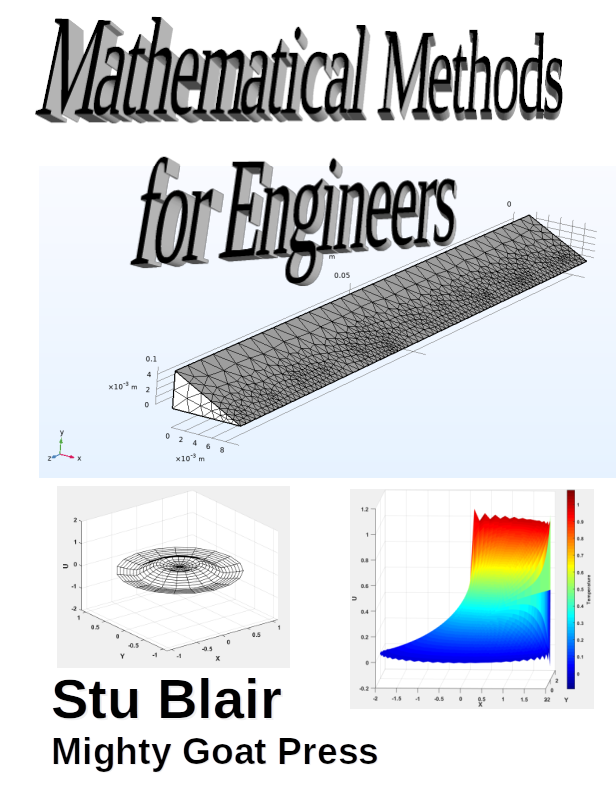
\includegraphics[width=1.7\textwidth]{cover3.png}
\end{figure}
\end{fullwidth}

% Front matter
\frontmatter

% r.1 blank page
%\blankpage


% v.2 epigraphs
\newpage\thispagestyle{empty}
\vfill
\openepigraph{%
When in doubt, multiply both sides by an orthogonal function and integrate.
}{P.L. Chebyshev}

\vfill
\openepigraph{%
The purpose of computing is insight, not pictures.
}{L.N. Trefethen}


\vfill
\openepigraph{%
Never do a calculation until you already know the answer.
}{J.A. Wheeler}


% r.3 full title page
\maketitle


% v.4 copyright page
\newpage
\begin{fullwidth}
~\vfill
\thispagestyle{empty}
\setlength{\parindent}{0pt}
\setlength{\parskip}{\baselineskip}
Copyright \copyright\ \the\year\ \thanklessauthor
\par\smallcaps{Published by \thanklesspublisher}

%\par\smallcaps{tufte-latex.github.io/tufte-latex/}
%
%\par Licensed under the Apache License, Version 2.0 (the ``License''); you may not
%use this file except in compliance with the License. You may obtain a copy
%of the License at \url{http://www.apache.org/licenses/LICENSE-2.0}. Unless
%required by applicable law or agreed to in writing, software distributed
%under the License is distributed on an \smallcaps{``AS IS'' BASIS, WITHOUT
%WARRANTIES OR CONDITIONS OF ANY KIND}, either express or implied. See the
%License for the specific language governing permissions and limitations
%under the License.\index{license}

\par\textit{First printing, \monthyear}
\end{fullwidth}

% r.5 contents
\tableofcontents

\listoffigures

\listoftables

% r.7 dedication
%\cleardoublepage
%~\vfill
%\begin{doublespace}
%\noindent\fontsize{18}{22}\selectfont\itshape
%\nohyphenation
%Dedicated to the midshipmen of the United States Naval Academy; the future of our armed services and of %our country.
%\end{doublespace}
%\vfill
%\vfill


% r.9 introduction
\cleardoublepage
\chapter*{Preface}

The purpose of this text is to provide a concise reference for engineering students who would like to strengthen their conceptual understanding and practical proficiency in analytical and numerical methods in engineering.  The material is based on a sequence of two courses taught at the United States Naval Academy.  

\subsection*{Analytical Methods}

The first course is focused on analytical methods for linear ordinary and partial differential equations.  All students come into the course having taken a three-semester sequence of calculus along with a course in ordinary differential equations.  The analytical methods portion briefly reviews methods for constant coefficient linear equations and proceeds to methods for non-constant coefficient ODEs including Cauchy-Euler equations, power series methods, and the method of Frobenieus.  After a review of Fourier Series methods and an introduction to Fourier-Legendre and Fourier-Bessel expansions we thoroughly explore solutions to second-order, linear, partial differential equations.  Since many students are also studying nuclear engineering, there is a heavy focus on addressing boundary value problems in cylindrical and spherical coordinate systems that are applicable to other topics of interest such as reactor physics.  There is also heavy emphasis on heat transfer applications that students will see later on in their undergraduate curriculum.

The materials presented are based heavily on Professor Dennis Zill's excellent book.\cite[-3cm]{zill2020advanced} We lightly select from chapters 1-3 for review; chapter 5 for series solution methods; and chapters 12-14 for Fourier Series and solutions to linear boundary value problems.  

What distinguishes this course from Prof Zill's work is the explicit incorporation of computational tools in the solution process.  These ``semi-analytical methods'' are presented here in MATLAB\cite[-3.75cm]{matlab} owing to the students preparation with that tool.  Other open-source tools like Octave\cite[-3.5cm]{octave} and Python,\cite[-1cm]{10.5555/1593511} of course, could be used. 

\subsection*{Numerical Methods}
The second course is focused on numerical methods for a variety of applications relevant to the physical sciences.  Prerequisites for this course include a three-semester sequence of calculus followed by a course in ordinary differential equations. Students also are required to have taken an introductory programming course where they have gained experience using the MATLAB programming environment.  A majority of the students who have taken this course have also taken the Analytical Methods course previously, although it is not a requirement.  

The course starts with an introduction to number representation on a computer and reviews the basics of linear algebra.  This is followed by treatment of algorithms for solving nonlinear equations and systems of equations.  For linear systems of equations, both direct and iterative methods are described; this includes treatment of sparse linear systems and preconditioning for iterative algorithms.  Least squares curve fitting is described in some detail as is interpolation with Lagrange polynomials.  Numeric differentiation is treated with both finite difference formulas as well as differentiation with Lagrange polynomials.  Several algorithms for numeric integration are described along with a fairly complete derivation of Gauss quadrature.  Several Runge-Kutta methods are illustrated for solving initial value problems, this includes a description of embedded RK methods with adaptive time-stepping.  Boundary value problems are solved using the shooting method, finite difference methods, and finite element methods.  A moderately detailed derivation of the Galerkin formulation of the method of weighted residuals is used to introduce Finite element methods.  The course is finished with several computational workshops using COMSOL, the details of which are not treated in this manuscript. 

The materials presented are based heavily on the excellent textbook by Prof Amos Gilat and Prof Vish Subramaniam.\cite{gilat}  The review is taken from selected portions of chapter 1 and 2; methods for solving non-linear and linear equations from chapter 3 and 4; curve fitting, interpolation, differentiation and integration are derived, in part, from chapters 6, 8, and 9; and most of the initial and boundary value problem examples are taken from chapters 10 and 11.

Several topics have been added to the treatment of Gilat and Subramaniam in an effort to selectively add depth and, in a few cases, provide updates to highlight tools available with more recent releases of MATLAB.  Depth is added with the treatment of sparse matrices and preconditioned iterative solution schemes for linear systems of equations; a more detailed derivation of Gauss quadrature is provided; several more Runge-Kutta methods are shown for solving initial value problems including implicit and embedded RK methods.  The treatment of finite element methods is based, in part, on the exposition of and lessons learned from Prof Young Kwon from the Naval Postgraduate School.\cite{kwon2018finite} 

This course is intended to serve scientists and engineers who will use numerical methods \emph{as a tool} in the context of computational problems that they may face.  As a consequence, a fairly pragmatic approach is taken with many of the derivation details summarized or, in some cases, skipped altogether.  Many methods are described not derived and theorems are used and applied, not proven.  I hope that any mathematician with the patience to read through these pages will graciously forgive me and, if needed, look for a different reference.

%%
% Start the main matter (normal chapters)
\mainmatter

\part{Introduction and Review}

\chapter{Lecture 1 - Introduction, Definitions and Terminology}
\label{ch:lec1}%<< think of better label and chapter names
\section{Objectives}
The objectives of this lecture are:
\begin{itemize}
\item Provide an overview of course content.
\item Define basic terms related to differential equations.
\item Provide examples of classification schemes for differential equations.
\end{itemize}

\section{Course Introduction}
This course is intended as a one-semester introduction to partial differential equations.  It is assumed that all students have a thorough background in single- and multi-variable calculus as well as differential equations.  The first few lectures comprise a review of the portions of differential equations on which this course most heavily relies.  This is followed by a treatment of power series methods and the method of Frobenius.  These are needed so that students will understand the origins of Legendre polynomials and Bessel functions that will be used in the solution of boundary value problems in spherical and cylindrical coordinates respectively.

\newthought{The main body} of material deals with the solution of (mostly homogeneous) boundary value problems---wave equation, heat equation, and Laplace equation---in rectangular, polar/cylindrical, and spherical coordinate systems.  For this, a preparatory review of Fourier series expansions along with Fourier-Legendre and Fourier-Bessel expansions is included  along with a leavening of Sturm-Liouville theory in boundary value problems.  The rest is a problem-by-problem tour of methods and analysis with heavy emphasis on heat transfer and nuclear engineering applications.

\section{Classification of Differential Equations}
It is important to be able to classify differential equations.  In this class we will learn a variety of techniques to find a function that satisfies a differential equation along with its boundary or initial conditions.\sidenote{Consider the differential equation: $\frac{du}{dx} = ux$.  The variable $u$ stands for the function, $u(x)$, that satisfies the equation; $u$ is also referred to as the \textbf{dependent variable}.  The variable $x$ is the \textbf{independent variable}.  By convention we will use the variables $x,y,z$ and $r,\theta,\phi$ as spatial independent variables and $t$ as an independent variable for time-dependent problems.  We will use many other letters to denote dependent variables but most commonly $u,f,g,h,v$ and $\psi$. When working through the separation of variables process we will also use $F,G,$ and sometimes $H$.} The techniques we learn in this class are tailored for specific classes of problems; you classify the problem and that tells you what method to use.  If you improperly classify the equation, you will likely use an inappropriate method and may have trouble figuring out why you cannot solve the problem.  
\subsection{Classification by Type and Order} \index{ordinary differential equation} \index{partial differential equation}
We shall start with the easiest classification categories: type and order.  There are two \emph{types} of differential equations that we will consider: \emph{ordinary differential equations} and \emph{partial differential equations.}  
\newthought{In an ordinary} differential equation\marginnote{\textbf{Example ODE:} $$\frac{d^2u}{dt^2}+t \frac{du}{dt}=3e^{-t}$$  There is one independent variable, $t$}, there is only one independent variable.  In a \emph{partial} differential equation,\marginnote{\textbf{Example PDE:} $$\frac{\partial^2u}{\partial x^2} + \frac{\partial^2u}{\partial y^2} = 0 $$ There are two independent variables, $x,$ and $y$.} there are multiple independent variables and consequently derivatives of the dependent variable will require partial derivatives.
\newthought{The order of} a differential equation is the order of the highest derivative in the equation.  This is typically not confusing for students. If anything needs to be added here it is to be mindful of the difference between a higher order derivative and an exponent.  For example, in the second order, non-linear, ordinary differential equation shown below, 
$$ \frac{d^2u}{dx^2}+5\left(\frac{du}{dx} \right)^3 - 4u = e^{x}  $$
it isn't \emph{too} hard to realize that the ``3'' is an exponent and the ``2'' denotes a second derivative. Still, be mindful.   

\subsection{Classification by Linearity} \index{linear ordinary differential equation}
An $n$\textsuperscript{th} order ordinary differential equation is said to be \emph{linear} when it can be written in the form shown in Equation \ref{eq:lin_ode}:\marginnote{\textbf{Note:} The notation $u^{(n)}$ and $u^{(n-1)}$ refer to the $n$\textsuperscript{th} and $(n-1)$\textsuperscript{th} derivative of $u$ respectively.}
\begin{equation}
a_n(x)u^{(n)}+a_{n-1}(x)u^{(n-1)}+\cdots+a_1(x)^{\prime}+a_0(x)u = g(x)
\label{eq:lin_ode}
\end{equation}
The key features that you should note in the form of Equation \ref{eq:lin_ode} are:
\begin{enumerate}
\item The \emph{dependent} variable and \emph{all of its derivatives} are of the first degree; that is, the power of each term involving $u$ is 1.
\item The coefficients of each term, $a_n(x)$, depend at most on the \emph{independent} variable(s).
\end{enumerate}
A lot of students struggle with discriminating between linear and nonlinear ODEs but it really is as simple as checking these two features.\marginnote{\textbf{Why is this important?} Most of the techniques we will learn in this course \emph{depend} upon the fact that the equation we are trying to solve is \emph{linear}.  In \emph{``the wild''} you may be presented with (or, more likely \emph{derive}) an equation and may not be explicitly told whether or not the equation is linear.  If the equation is \textbf{not} linear you will find that most of the tools you learn in this course will not be applicable; you will most likely need to use a numerical method. You need to be able to tell the difference so you know what tools to use.}  If both conditions are satisfied: the equation is linear.  If not, the equation is nonlinear.  As examples, Equation \ref{eq:nonlin_1} violates the first criterion; Equation \ref{eq:nonlin_2} violates the second.
\begin{equation}
\frac{d^2u}{dx^2}+u^2 = 0 
\label{eq:nonlin_1}
\end{equation}
\begin{equation}
\frac{d^3u}{dx^3}-5u\frac{du}{dx}=x
\label{eq:nonlin_2}
\end{equation}
\section{Verification of an Explicit Solution} 
A solution in which the dependent variable is expressed solely in terms of the independent variable and constants is said to be an \emph{explicit} solution.\marginnote{\textbf{Example explicit solution:} $u(x) = f(x)$.} Otherwise, the solution is \emph{implicit}.\marginnote{\textbf{Example implicit solution:} $G(x,u) = 0$} 

\newthought{In this class} we will mainly be interested in finding explicit solutions to differential equations that we are given or have derived.  There are some cases, however, where we are given a function and we wish to verify that it is a solution to a given differential equation.  To do this, we simply ``plug'' the equation into the differential operator and verify that an identity is derived.

\begin{example}
\textbf{Example:} Verify that $u = \frac{6}{5} - \frac{6}{5}e^{-20t}$ is a solution to:
$$\frac{du}{dt} + 20u = 24$$
\vspace{0.5cm}
\textbf{Solution:}
Since $\frac{du}{dt} = \frac{d}{dt}(\frac{6}{5} - \frac{6}{5}e^{-20t}) = 24e^{-20t}$, we can see that:
\begin{align*}
\frac{du}{dt} + 20u &= 24e^{-20t} + 20(\frac{6}{5} - \frac{6}{5}e^{-20t}) \\
&= 24e^{-20t} + 24 - 24e^{-20t} \\
&=24
\end{align*} 
which is the expected identity.
\end{example} 


\chapter{Lecture 2 - Separable and Linear 1st order Equations}
\label{ch:lec2}
\section{Objectives}
The objectives of this lecture are:
\begin{itemize}
\item Define and describe the solution procedure for \emph{separable} first order equations.
\item Define and demonstrate the solution procedure for \emph{linear} first order equations.
\end{itemize}

\section{Separable Equations} \index{separable differential equation}
A first order differential equation of the form shown below:
\begin{equation}
\frac{du}{dx} = g(u)h(x)
\label{eq:separable}
\end{equation}
is said to be \emph{separable} or have \emph{separable variables.}\marginnote[-1.5cm]{\textbf{Note:} there is \textbf{no} requirement that the 1st order equation be \emph{linear}.  This is the only technique that we will study in this course that can be applied to nonlinear equations.} 

\newthought{The solution method} for separable equations is, in principle, simple.  For the separable differential equation given in Equation \ref{eq:separable} we would separate and integrate:

\begin{align*}
\frac{du}{dx} &= g(u)h(x) \\
\frac{du}{g(u)} &= h(x) dx \\
\int \frac{1}{g(u)} \ du &= \int h(x) \ dx 
\end{align*}
\marginnote[-3.5cm]{\textbf{Note:} there are at least two complications here.
\begin{enumerate}
\item The solution you thus derive may be either implicit or explicit.  An implicit solution is, as a practical matter, fairly inconvenient to deal with; and
\item It may not be possible to carry out the integrals analytically. 
\end{enumerate}
Nonetheless, we shall carry on and give it a try anyway.  
}
Generally speaking, one of your first checks for a first order equation should be: is it separable?  If so, you should separate the variables and solve.  The examples below are intended to illustrate the method.  Note that in the final example, the integral cannot be done analytically.
\begin{example}[h!]
Solve the following separable, first order differential equations
.
\textbf{Example 1:} 
\begin{align*}
\frac{du}{dx} &= \frac{u}{1 + x} \\
\frac{du}{u} &= \frac{dx}{1+x} \\
\int \frac{d}{u} &= \int \frac{dx}{1+x} \\
\ln{|u|} + c_1 &= \ln{|1+x|} + c_2 \\
|u| &= e^{\left[\ln{|1+x|} + c_3\right]}\\
    u(x)&= c|1+x|
\end{align*}

\end{example}

\begin{example}[h!]
\textbf{Example 2:}
\begin{align*}
\frac{du}{dx} &= -\frac{x}{u} \\
\int u \ du &= -\int x \ dx \\
\frac{u^2}{2} &= -\frac{x^2}{2}+c \\
u(x) &= \sqrt{c - x^2}
\end{align*}
\end{example}

\begin{example}[h!]
\textbf{Example 3:}
Solve the first order initial value problem shown below:
\begin{equation*}
\frac{du}{dx} = e^{-x^2}, \ \ u(2) = 6, \ \ 2 \le x < \infty
\end{equation*}
\begin{align*}
du &= e^{-x^2}\ dx \\
\int_2^{x} \frac{du}{dt} \ dt &= \int_{2}^{x} e^{-t^2} \ dt \\
u(x) - u(2) &= \int_{2}^{x} e^{-t^2} \ dt \\
u(x) &= 6 + \int_{2}^{x} e^{-t^2} \ dt
\end{align*}
where we have used the dummy variable $t$ in the integrals; the last integral will need to be evaluated numerically.

\end{example}

\section{Linear Equations}
A first-order differential equation of the form:
\begin{equation}
a_1(x)\frac{du}{dx} + a_0(x)u = g(x)
\label{eq:lin_first_order}
\end{equation}
is said to be a first order \emph{linear equation} in the dependent variable $u$.\marginnote[-2.0cm]{\textbf{Note:} it is sometimes customary to write the differential equation in \emph{operator form} where the differential operator, $\mathcal{L}=a_1(x) \frac{d}{dx} + a_0(x)$, is applied to the function $u(x)$ to get $g(x)$; $\mathcal{L}u(x) = g(x)$ }
When $g(x) = 0$, the first-order linear equation is said to be \emph{homogeneous}; otherwise it is \emph{non-homogeneous}.\marginnote{Notice that $g(x)$ is the only term in Equation \ref{eq:lin_first_order} that does \underline{\textbf{not}} include $u$ or any of its derivatives.}

\newthought{When solving} equations of this type it is customary to express it in the \textbf{standard form}: \index{standard form, first order linear}
\begin{equation}
\frac{du}{dx}+P(x)u = f(x)
\label{eq:first-order-linear-standard-form}
\end{equation}  
The method for solving this equation makes use of the \underline{\emph{linearity}} property\marginnote{When we say an operator is \textbf{linear}, what we mean is that the following relationships must hold:
\begin{enumerate}
\item $\mathcal{L}(\alpha u) = \alpha \mathcal{L}(u)$
\item $\mathcal{L}(u + v) = \mathcal{L}(u) + \mathcal{L}(v)$
\end{enumerate}
for functions $u$,$v$ and scalar constant $\alpha$.  Think of this as a \emph{definition} of linearity.} and we express the solution in the following way: $u(x) = u_c(x) + u_p(x)$. Inserting this into Equation \ref{eq:first-order-linear-standard-form} gives us:

\begin{multline}
\frac{d}{dx}[u_c + u_p] + P(x)[u_c + u_p] = \\
\left[\frac{du_c}{dx}+P(x)u_c \right] + \left[\frac{du_p}{dx}+P(x)u_p \right] = f(x) 
\label{eq:lin-first-order1}
\end{multline}
where $u_c(x)$ is the solution to the \emph{associated homogeneous problem}:\marginnote{The linear operator here is: $\mathcal{L}=\frac{d}{dx} + P(x)$.  Equation \ref{eq:fol_complementary} says $\mathcal{L}u_c = 0$; Equation \ref{eq:fol_particular} says $\mathcal{L}u_p = f(x)$; Equation \ref{eq:lin-first-order1} says that $\mathcal{L}(u_c+u_p) = 0+f(x) = f(x)$.}
\marginnote[0.25cm]{What might trouble you now is: if we have $u_p$, is this not a solution to Equation \ref{eq:first-order-linear-standard-form}?  Why do we need $u_c$?  The next thing that should trouble you is that if $u_p$ is a solution, by the linearity property of $\mathcal{L}$, so is $u_p$ plus \emph{any} constant multiple of $u_c$.  The solution is not \emph{unique}}
\marginnote[0.25cm]{This will all be resolved when we recall that $u_c$ will have an arbitrary constant through which we will be able to say that $u = u_c + u_p$ is a function describing \emph{all} possible solutions of Equation \ref{eq:first-order-linear-standard-form} and the arbitrary constant(s) in $u_c$ will be set so as to uniquely satisfy a given initial/boundary condition.}
\begin{equation}
\frac{du_c}{dx}+P(x)u_c = 0
\label{eq:fol_complementary}
\end{equation}
and $u_p(x)$ is a solution to:
\begin{equation}
\frac{du_p}{dx}+P(x)u_p = f(x)
\label{eq:fol_particular}
\end{equation}
We can see that Equation \ref{eq:fol_complementary} is separable:
\begin{align*}
\frac{du_c}{dx}+P(x)u_c &= 0 \\
\frac{du_c}{u_c} &= -P(x) \ dx \\
\ln{u_c} + C &= -\int P(x) \ dx \\
u_c(x) &= e^{-\int P(x) \ dx + C_1} \\
u_c(x) &= e^{-\int P(x) \ dx}e^{C_1} \\
u_c(x) &=Ce^{-\int P(x) \ dx}
\end{align*}
where $C = e^{C_1}$.\marginnote{\textbf{Note:} Going forward, we will desist in making such piddling distinctions between constants.  $C_1$ is an arbitrary constant, $e^{C_1}$ is still an arbitrary constant.  There is no real difference between $C_1$ and $C$ and, in this author's humble opinion, they do not rate different symbols.}

\newthought{We need to find} a solution $u_p(x)$ to Equation \ref{eq:fol_particular}.  The technique we will use is called \emph{variation of parameters}.  It consists of looking for a solution in the form $y_p(x) = v(x)u_1(x)$, where $u_1(x) = e^{-\int P(x) \ dx}$ which is $u_c(x)$ with the arbitrary constant set to 1 and $v(x)$ might be thought of as some kind of weighting or \emph{variational} function.
\index{variation of parameters}

\vspace{0.25cm}

\noindent We will insert this proposed form of $y_p(x)$ into Equation \ref{eq:fol_particular}:
\begin{equation*}
\frac{d(vu_1)}{dx} + P(x)\left[v(x)u_1(x)\right]=f(x)
\end{equation*}
We apply the product rule to the first term and re-arrange to get:
\begin{align*}
u_1(x)\frac{dv}{dx}+ v(x)\frac{du_1}{dx} + P(x)\left[v(x)u_1(x)\right] &= f(x) \\
v(x)\underbrace{\left[\frac{du_1}{dx}+P(x)u_1(x) \right]}_{\textbf{= 0}}+u_1(x)\frac{dv}{dx} &= f(x) \\
u_1(x)\frac{dv}{dx} &= f(x)
\end{align*}
In the last line we can observe that the equation is \emph{separable} and thus solve accordingly:
\begin{align*}
v(x) &= \int \frac{f(x)}{u_1(x)} \ dx \\
     &= \int e^{\int P(x) \ dx}f(x) \ dx
\end{align*}
Now that we know what $v(x)$ must be, we can combine this with $u_1(x)$ to get $u_p(x)$:
\begin{equation}
u_p(x) = e^{-\int P(x) \ dx}\left[\int e^{\int P(x) \ dx}f(x) \ dx \right]
\label{eq:fol-particular-sol}
\end{equation}
Equation \ref{eq:fol-particular-sol} is messy and perhaps a bit scary but given definitions of $P(x)$ and $f(x)$ we might hope we can solve it anyway.  We now have expressions for both $u_c$ and $u_p$ and we combine them to form the solution for the first-order linear equation:
\begin{equation}
u(x) = Ce^{-\int P(x) \ dx} + e^{-\int P(x) \ dx} \left[e^{\int P(x) \ dx} f(x) \ dx \right]
\label{eq:fol-solution}
\end{equation}

\section{Method of Solution} \index{method of solution, first order linear}
In summary, once we have identified a problem to be first-order and linear, we will solve the problem using the following steps:
\begin{enumerate}
\item Write the equation in standard form (Equation \ref{eq:first-order-linear-standard-form})
\item Determine the integrating factor $\mu = e^{-\int P(x) \ dx}$.
\item Solve for the general solution $u(x)$ using Equation \ref{eq:fol-solution}.
\item Apply initial/boundary condition if given.
\end{enumerate}

\vspace{1cm}
\underline{\textbf{Example:}}
Solve the problem:
$$\frac{du}{dx}+u=x, \ \ u(0) = 4$$

\textbf{Step \#1:}
The equation is already in standard form.

\vspace{0.25cm}
\textbf{Step \#2:} Find the integrating factor $\mu$.

$$mu = e^{-\int P(x) \ dx} = e^{-\int 1 \ dx} = e^{-x}$$

\vspace{0.25cm}
\textbf{Step \#3:} Solve for the general solution $u(x)$ using Equation \ref{eq:fol-solution}
\marginnote[1.25cm]{$\leftarrow$ For the integral $\int e^x x \ dx$ we need to use integration by parts.}
\begin{align*}
u(x) &= Ce^{-x}+e^{-x}\int e^{x}x \ dx \\
&= Ce^{-x} + e^{-x}\left[xe^{x}-e^{x} \right] \\
&= Ce^{-x} + x - 1
\end{align*}

\vspace{0.25cm}
\textbf{Step \#4:} Apply initial/boundary conditions if given

\begin{align*}
u(0) &= Ce^{0} + 0 -1 \\
 &=C-1 = 4 \\
 \Rightarrow C &= 5 \\
 u(x) &= 5e^x+x-1
\end{align*}




\chapter{Assignment \#1}
\label{ch:ass1}
\begin{fullwidth}

State the order of the given ordinary differential equation and indicate if it is linear or non-linear.

\begin{enumerate}
\item $\left(1-x\right)u^{\prime \prime}-4xu^{\prime} + 5u = \cos{x}$
\vspace{1.0cm}
\item $t^5u^{(4)}-t^3u^{\prime \prime}+6u=0$
\vspace{1.0cm}
\end{enumerate}

\noindent Verify the indicated function is an explicit solution of the given differential equation.
\begin{enumerate}[resume]
\item $2u^{\prime}+u=0, \ \ u=e^{-x/2}$
\vspace{1.0cm}
\item $u^{\prime \prime} - 6u^{\prime}+13u=0, \ \ u=e^{3x}\cos{2x}$
\vspace{1.0cm}
\end{enumerate}

\noindent Solve the given differential equation by separation of variables.
\begin{enumerate}[resume]
\item $\frac{du}{dx}=\sin{5x}$
\vspace{1.0cm}
\item $dx + e^{3x}du = 0$
\vspace{1.0cm}
\item $\frac{dS}{dr} = kS$
\vspace{1.0cm}
\item $\frac{du}{dx} = x\sqrt{1-u^2}$
\vspace{1.0cm}
\end{enumerate}

\noindent Find an explicit solution of the given initial-value problem.
\begin{enumerate}[resume]
\item $x^2 \frac{du}{dx}=u-xu, \ \ u(-1)=-1$
\vspace{1.0cm}
\end{enumerate}

\noindent Find the general solution of the given differential equation.
\begin{enumerate}[resume]
\item $\frac{du}{dx} + u = e^{3x}$
\vspace{1.0cm}
\item $u^{\prime} + 3x^2u = x^2$
\vspace{1.0cm}
\item $x\frac{du}{dx}-u=x^2\sin{x}$
\end{enumerate}

\end{fullwidth}

\chapter{Lecture 3 - Theory of Linear Equations}
\label{ch:lec3}
\section{Objectives}
The objectives of this lecture are:
\begin{itemize}
\item Introduce several theoretical concepts relevant to initial value problems and boundary value problems.
\item Demonstrate use of the Wronskian to determine linear independence of solutions.
\item Present some important theorems and definitions relevant to the theory of linear ordinary differential equations.
\end{itemize}

\section{Initial Value Problems} \index{initial value problem}

For a linear differential equation, an n\textsuperscript{th}-order initial value problem (IVP) is given by the following governing equation and initial conditions:
\begin{multline}
\text{Governing Equation: }a_n(x)\frac{d^n u}{dx^n}+a_{n-1}\frac{d^{n-1}u}{dx^{n-1}}+\cdots \\+a_1(x)\frac{du}{dx}+a_0(x)u=g(x)
\label{eq:ivp-ge}
\end{multline}
\begin{equation}
\text{Initial Conditions: }u(x_0)=u_0, \ u^{\prime}(x_0)=u_1,\dots,u^{(n-1)}(x_0)=u_{n-1}
\label{eq:ivp-ics}
\end{equation}
\marginnote[-1.5cm]{\textbf{Note:} for an initial value problem, all of the initial conditions are provided at the same value of $x$; in accordance with custom we call this $x_0$.  The name \emph{initial} condition gives the implication that these conditions are at some ``end'' of the interval (beginning, left side, whatever) and in all examples and exercises in this text this is indeed the case.  It is not, however, a requirement.}
\noindent \newthought{We seek a} function defined on some interval containing $x_0$ that satisfies the differential equation with $n$ conditions applied.\marginnote{Generally for an n\textsuperscript{th}-order IVP you will need $n$ conditions.} The theorem below, which we will use by \emph{citing} rather than \emph{proving}, gives us assurance that, subject some fairly reasonable assumptions, such a solution will exist.  

\begin{theorem}[Existence and Uniqueness for IVPs]
If $a_n(x),a_{n-1}(x),\dots,a_1(x),a_0(x)$ and $g(x)$ are continuous on an interval $\mathcal{I}$, and if $a_n(x) \ne 0$ for every $x \in \mathcal{I}$, and if $x_0$ is any point in this interval, then a solution $u(x)$ of the IVP exists on the interval and it is unique.
\label{thm:IVP-exist-and-unique}
\end{theorem}
\newthought{For this class} we will adopt a fairly operational definition of continuity: if you can draw the function throughout the specified interval without picking up your pencil or without diverging to infinity, then the function is continuous. 
\index{continuity} 

Consider, as an example, the following initial value problem:
\begin{equation}
u^{\prime \prime}-4u = 12x, \ \ u(0)=4, \ u^{\prime}(0)=1
\label{eq:lec3-ex1}
\end{equation}
This IVP satisfies the conditions of Theorem \ref{thm:IVP-exist-and-unique} since all of the coefficients and $g(x)$ are continuous and $a_2$ is constant and nonzero; hence a unique solution exists on any interval and that solution is unique.\marginnote[-1.5cm]{Take a moment to verify that $u(x)=3e^{2x}+e^{-2x}-3x$ satisfies both the governing equation and initial conditions given in Equation \ref{eq:lec3-ex1} and thus is \emph{the} unique solution to this IVP.}

Here is an IVP that does \emph{not} satisfy the criteria of Theorem \ref{thm:IVP-exist-and-unique}:
\begin{equation}
x^2u^{\prime \prime} - 2xu^{\prime}+2u=6, \ \ u(0)=3, \ u^{\prime}(0)=1
\label{eq:lec3-ex2}
\end{equation}
\noindent In this case, the coefficients and $g(x)$ are all continuous but $a_2(x)$ is equal to zero at $x=0$.  This might not be a problem---i.e. if $x=0$ is not in the interval of interest for the IVP then we are okay---but since $x_0=0$, $x=0$ \emph{must} be in the domain for the theorem to apply.  So we have no assurances that a solution exists or, if a solution does exist, it may not be unique.\marginnote[-1.5cm]{You should take a moment to verify that $u(x)=cx^2+x+3$ is a solution for the IVP given in Equation \ref{eq:lec3-ex2} for \emph{any} choice of parameter $c$.}

\section{Boundary Value Problems} \index{boundary value problem}
For this section let us, without undue loss of generality, consider a 2\textsuperscript{nd}-order boundary value problem (BVP):\marginnote{Almost all of the applications we will consider for this class will involve 2\textsuperscript{nd}-order operators.  The way we derive important boundary-value problems from underlying physical laws like conservation of mass and conservation of energy lead to them being 2\textsuperscript{nd}-order.  You should think about this while you are sitting in your fluid dynamics class and equations are being derived for conservation of mass and momentum for viscous incompressible fluid flow or when you are sitting in heat transfer class and the heat equation is being derived from conservation of energy principles.  Probably the most obvious counterexample is beam theory which involves a 4\textsuperscript{th}-order operator.}
\begin{equation}
\text{Governing Equation: }a_2(x)\frac{d^2u}{dx^2}+a_1(x)\frac{du}{dx}+a_0(x)u=g(x) 
\end{equation}
\begin{equation}
\text{Boundary Conditions: } y(a)=y_0, \ \ y(b)=y_1, \ \ a \ne b
\end{equation}

\newthought{Depending on the} boundary conditions, BVPs may have no solutions, one unique solution, or infinitely many solutions.

\vspace{1.0cm}
\noindent \underline{\textbf{Example:}} The equation $u^{\prime \prime}+16u = 0$ has the general solution $u(t) = c_1 \cos{(4t)}+c_2 \sin{(4t)}$.  Consider the three different sets of boundary conditions provided below:
\begin{enumerate}[label=\alph*)]
\item $u(0)=0, \ \ u(\pi/2)=0$.
Application of the first boundary condition gives us $c_1(1)+c_2(0)=0 \Rightarrow c_1 = 0$.  The second boundary condition is $c_2\sin{(2 \pi)} = 0,$ which is true for \emph{any} value of $c_2$.  Therefore there problem has infinitely many solutions.
\item $u(0)=0, \ \ u(\pi/8)=0$.
The first boundary condition again gives us $c_1=0$; the second condition $c_2\sin{(4 \frac{\pi}{8})}=0$ is only satisfied if $c_2=0$.  Thus $c_1 = c_2 = 0$; only the trivial solution, $u=0$, satisfies both the differential equation and boundary conditions.  This is not a very interesting solution but at least it \emph{is a solution} so we will take this as an example of a BVP having a unique solution.\marginnote{For applications, we will generally be only interested in \emph{non-trivial} solutions; that is, solutions that are not identically equal to zero.}
\item $u(0)=0, \ \ u(\pi/2)=1$.
In this case, again $c_1=0$ from the first boundary condition.  This leaves the second boundary condition: $c_2 \sin{\left(4 \frac{\pi}{2}\right)} = c_2(0) = 1$ which cannot be satisfied for any value of $c_2$.  In this case \emph{no} solution exists.

\end{enumerate}

\section{Superposition and Linear Dependence} \index{superposition} \index{linear dependence}
In this section some important theorems regarding IVPs and BVPs will be presented.  No attempt will be made to prove these theorems; we will simply take these theorems as facts that are relevant for this course that you should try to understand as best you can.

\begin{theorem}[Superposition Principle for Homogeneous Equations]
Let $u_1,u_2,\dots,u_k$ be solutions of a homogeneous n\textsuperscript{th}-order linear differential equation.  Then any linear combination of those solutions 
$$u = c_1u_1+c_2u_2+\cdots+c_ku_k$$where $c_1,c_2,\dots,c_k$ are arbitrary constants, is also a solution.
\end{theorem}
\marginnote[-3.0cm]{\textbf{Note:} It is essential that \emph{both} the governing equation and given conditions (boundary or initial) for the linear differential equation are homogeneous.  As a reminder, this means that \emph{all} terms in the governing equation and boundary conditions must either a) involve the dependent variable or one of its derivatives; or b) be equal to zero.} 
As an example, If we denote the linear homogeneous differential equation as $\mathcal{L}$, then $\mathcal{L}(u_i) = 0$ for any $i \in [1,2,\dots,k]$.  By the linearity property of $\mathcal{L}$, for any constants $\alpha$ and $\beta$:
\begin{align*}
\mathcal{L}(\alpha u_i + \beta u_j) &=  \alpha \mathcal{L}(u_i) + \beta \mathcal{L}(u_j)\\
&= \alpha(0) + \beta(0) \\
&= 0
\end{align*}
thus $\alpha u_i + \beta u_j$ is a solution.

\begin{theorem}[Linear Dependence / Independence of Functions]
A set of functions $f_1(x),f_2(x),\dots,f_k(x)$ is said to be \emph{linearly dependent} on an interval $\mathcal{I}$ if there exist constants $c_1,c_2,\dots,c_k$, \emph{not \underline{all} of which are zero}, such that
$$c_1f_1(x) + c_2f_2(x)+\cdots+c_kf_k(x) = 0$$
\noindent for every $x \in \mathcal{I}$.  If the set of functions is \emph{not} linearly dependent, it is linearly independent.
\label{th:linear-dep}
\end{theorem} 
\marginnote[-1.75cm]{\textbf{Question: }What if a member of the set of functions is $f(x)=0$? 

\vspace{0.25cm}

\noindent\textbf{Answer:} The set will no longer be linearly independent.  The trivial function $f(x)=0$ is not linearly independent from \emph{anything}.}
Repeatedly throughout this course we will want to clarify whether or not two or more functions are linearly independent of each other.  I think most engineers have a general idea of what it is we \emph{mean} when we say two functions are linearly independent or dependent but Theorem \ref{th:linear-dep} specifies what these things mean \emph{mathematically}.  
\newthought{We need a test} to help us determine whether or not the members of a set are linearly independent. This will be especially important as we evaluate solutions to a linear homogeneous differential equation.  Even if you are the sort of savant who can, by inspection, always detect linear dependence, you might have a hard time convincing your friends that your assessment is always correct.  Luckily, there is a theorem that provides a suitable test that can serve as irrefutable evidence of the state of linear dependence/independence of functions.

\begin{theorem}[Criterion for Linearly Independent Solutions]
Let $u_1,u_2,\dots,u_n$ be solutions of a homogeneous linear n\textsuperscript{th}-order differential equation defined on an interval $\mathcal{I}$.  Then the set of solutions is linearly independent on the interval if and only if the Wronskian of the solution is non-zero for every $x \in \mathcal{I}$.  
\end{theorem}\index{Wronskian}
The Wronskian is a function that takes functions as arguments and returns a scalar numeric quantity and is defined in Equation \ref{eq:Wronskian-def}:\begin{equation}
W(u_1,u_2,\dots,u_n)=
\begin{vmatrix}
u_1 & u_2 & \cdots & u_n \\
u^{\prime}_1 & u^{\prime}_2 & \cdots & u^{\prime}_n \\
\vdots & \vdots & \vdots & \vdots \\
u^{(n-1)}_1 & u^{(n-1)}_2 & \cdots & u^{(n-1)}_n
\end{vmatrix}
\label{eq:Wronskian-def}
\end{equation}
where $|\cdot|$ denotes the matrix determinant.  For large values of $n$ this is difficult to calculate but, for the case $n=2$, engineering students should be familiar with the formula:\marginnote{Students of this class should also be able to find determinants for 3x3 matrices.  If you have forgotten that formula, consult your favorite textbook or online resource for a reminder.}
\begin{equation}
W(u_1,u_2) = 
\begin{vmatrix}
u_1 & u_2 \\
u^{\prime}_1 & u^{\prime}_2 \\
\end{vmatrix}
= u_1 u^{\prime}_2 - u^{\prime}_1 u_2
\end{equation}

\vspace{0.5cm}

\noindent\textbf{\underline{Example:}} Show that the functions $u_1 = e^{3x}$ and $u_2=e^{-3x}$ are linearly independent solutions to the homogeneous linear equation $u^{\prime \prime}-9u=0$ for every $x \in (-\infty,\infty)$.

\noindent\textbf{\underline{Solution:}} The Wronskian is given by:\marginnote{The reader should verify that both $u_1 = e^{3x}$ and $u_2=e^{-3x}$ satisfy the given differential equation.}
\begin{align*}
W &= 
\begin{vmatrix}
e^{3x} & e^{-3x} \\
3e^{3x} & -3e^{-3x}
\end{vmatrix} \\
&= e^{3x}\left(-3e^{-3x}\right) - 3e^{3x}\left(e^{-3x}\right) \\
&= 3e^{3x-3x} - 3e^{3x-3x} \\
&= 3 - 3 \\
&= 6
\end{align*}
\noindent Since $6 \ne 0$ for all $x \in (-\infty,\infty)$ the solutions are linearly independent.

\begin{definition}[Fundamental Set of Solutions]
Any set $\{u_1,u_2,\dots,u_n\}$ of $n$ linearly independent solutions of the homogeneous linear n\textsuperscript{th}-order differential equation on an interval is said to be a fundamental set of solutions on an interval $\mathcal{I}$.  
\end{definition}
\begin{theorem}[Existence of a Fundamental Set]
There exists a fundamental set of solutions for the homogeneous linear n\textsuperscript{th}-order differential equation on an interval $\mathcal{I}$.
\end{theorem}
\marginnote[-1.0cm]{\textbf{Note:} This is different than saying that a BVP or IVP has a solution.  This theorem is only referring to the differential equation; not the boundary or initial conditions.}

\begin{definition}[General Solution---Homogeneous Equation]
Let $\{u_1,u_2,\dots,u_n\}$ be a fundamental set of solutions to the homogeneous linear n\textsuperscript{th}-order differential equation defined on an interval $\mathcal{I}$, then the general solution is:
$$u(x) = c_1u_1(x)+c_2u_2(x)+\cdots+c_nu_n(x)$$
\end{definition}

\newthought{It is important} to understand from the above that:
\begin{itemize}
\item \emph{Any} possible solution to the homogeneous, linear, n\textsuperscript{th}-order differential equation can be constructed by setting the coefficients of the general solution; and
\item there is \textbf{no} solution that can be constructed from functions that are linearly independent from the general solution.
\end{itemize}

\section{General Solution for a Non-homogeneous Problem}
Recall: ``non-homogeneous'' for a linear n\textsuperscript{th}-order differential equation means that $g(x)\ne 0$.  If $u_p$ is any particular solution to the non-homogeneous, linear, n\textsuperscript{th}-order ODE on an interval $\mathcal{I}$ and $u_c = c_1u_1(x) + c_2u_2(x)+\cdots c_nu_n(x)$ is the general solution to the associated homogeneous ODE (called the \emph{complementary} solution) then the general solution to the non-homogeneous ODE is:
\begin{equation*}
u = u_c + u_p
\end{equation*}

\vspace{0.25cm}

\noindent\textbf{\underline{Example:}} By substitution it can be seen that $u_p = -\frac{11}{12}-\frac{1}{2}x$ is a particular solution to $u^{\prime \prime \prime}-6u^{\prime \prime} + 11u^{\prime} - 6u=3x$.  The general solution to the associated homogeneous problem is $u_c = c_1e^{x}+c_2e^{2x}+c_3e^{3x}$.\marginnote{You are, again, strongly encouraged to verify that $u_p$ satisfies the given equation and that $u_c$ satisfies the associated homogeneous equation.}  Consequently, the general solution to the linear non-homogeneous problem is:
\begin{align*}
u(x) &= u_c + u_p \\
&=c_1e^{x}+c_2e^{2x}+c_3e^{3x}-\frac{11}{12}-\frac{1}{2}x
\end{align*}


\chapter{Lecture 4 - Homogeneous Linear Equations with Constant Coefficients}
\label{ch:lec4}
\section{Objectives}
The objectives of this lecture are:
\begin{itemize}
\item Review the solution methodology for homogeneous linear equations with constant coefficients.
\item Illustrate this method with several examples.
\end{itemize}
\section{Introduction} \index{linear constant coefficient equations}
In this lecture we will review the well-trod ground of your differential equations class and remind ourselves how to solve linear, constant coefficient, homogeneous, n\textsuperscript{th}-order differential equations.  These equations have the general form shown in Equation \ref{eq:lcchnode}:
\begin{equation}
a_nu^{(n)}+a_{n-1}u^{(n-1)}+\cdots+a_1u^{\prime}+a_0u=0
\label{eq:lcchnode}
\end{equation}
\noindent where the coefficients are real and constant an $a_n \ne 0$.

\newthought{The basic strategy} is to assume the solution is of the form: $u(x)=e^{mx}$. For the case of 2\textsuperscript{nd}-order equations, we get:\marginnote{If $u(x) = e^{mx}$ then, of course, $u^{\prime} = me^{mx}$ and $u^{\prime \prime} = m^2e^{mx}$.}
\begin{align*}
a_2m^2e^{mx}+a_1me^{mx}+a_0e^{mx}&=0 \\
e^{mx}\left(a_2m^2+a_1m+a_0\right)
\end{align*}
\noindent where the last line above is called the auxiliary equation: \marginnote{Here we re-name the constants so Equation \ref{eq:aux-eqn} takes a familiar form.}
\begin{equation}
am^2+bm+c = 0
\label{eq:aux-eqn}
\end{equation}
From the well-known quadratic equation, solutions are: $m = \frac{-b\pm\sqrt{b^2-4ac}}{2a}$
Solution of this equation gives the following three cases:
\begin{enumerate}
\item \textbf{Distinct Real Roots}
In this case $m_1 \ne m_2$ and the general solution is of the form:
\begin{equation}
u(x) = c_1\underbrace{e^{m_1x}}_{u_1(x)}+c_2\underbrace{e^{m_2x}}_{u_2(x)}
\label{eq:dist-real-roots}
\end{equation}

Using tools from the last lecture you should recognize that $u_1(x)$ and $u_2(x)$ are linearly independent for all $x\in \left( -\infty,\infty\right)$, and thus form a fundamental set of solutions.  

\newthought{An important special case} is when $m_1$ and $m_2$ are roots of a positive real number and thus $m_1 = -m_2$.  This happens when the governing equation is of the form:

\begin{equation}
u^{\prime \prime} - k^2 u = 0
\end{equation}
The general solution is:
\begin{equation}
u(x) = c_1 e^{-kx} + c_2e^{kx}
\label{eq:sp-case-1-exp}
\end{equation}
\begin{marginfigure}
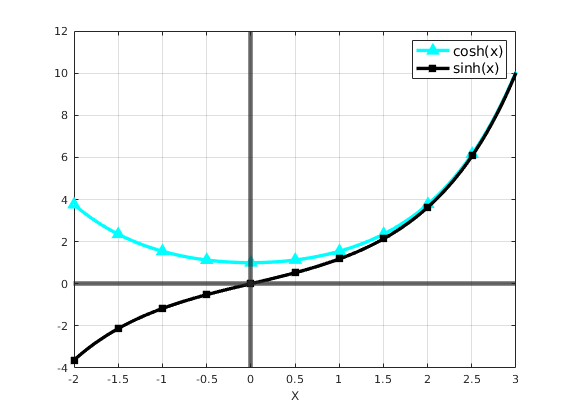
\includegraphics{cosh_and_sinh_plot.png}
\caption{Plot of $\cosh{x}$ and $\sinh{x}$}
\label{fig:cosh-and-sinh-plot}
\end{marginfigure}


For reasons that will become clear later in the course, it is sometimes useful to re-express the solution shown in Equation \ref{eq:sp-case-1-exp} in terms of the functions $\cosh{()}$ and $\sinh{()}$.  These functions are defined as linear combinations of exponentials as shown below and plotted in Figure \ref{fig:cosh-and-sinh-plot}.\marginnote{When applying boundary conditions and resolving unknown constants in a general solution to a differential equation, it is helpful that $\sinh{0} = 0$.  In contrast, neither $e^{x}$ nor $e^{-x}$ is equal to zero for finite values of $x$.}
\begin{align*}
\cosh{x} &= \frac{e^{x} + e^{-x}}{2} \\
\sinh{x} &= \frac{e^{x} - e^{-x}}{2}
\end{align*}



\item \textbf{Real Repeated Roots}
In this case $m_1 = m_2$.\marginnote{i.e. from the quadratic equation, $b^2-4ac = 0$}  One solution is:
\begin{equation}
u_1(x) = e^{m_1x}
\end{equation}

The other solution so derived is, of course, the same and thus we do not have two linearly independent solutions as required to form a fundamental set of solutions for a 2\textsuperscript{nd}-order linear homogeneous equation.  

\newthought{It can be shown} that a second linearly independent solution can be formed by multiplying $u_1(x)$ by the independent variable, $x$:\marginnote{This result is derived using a technique referred to as \emph{reduction of order}.  We will not take the time to cover it in this class (or in this book) but is concisely described in section 3.2 of Zill.  At a minimum you might at least confirm for yourself that a) $xu_1(x)$ is a solution to the equation; and b) use the Wronskian to confirm that it is linearly independent from $u_1(x)$.}
\begin{equation*}
u_2(x) = x u_1(x) = xe^{mx}
\end{equation*}
and thus the general solution for this case is:
\begin{equation}
u(x) = c_1e^{mx}+c_2xe^{mx}
\label{eq:rep-real-roots}
\end{equation}

\item \textbf{Conjugate Complex Roots}
In this case the discriminant, $b^2-4ac$, is negative so its square root is imaginary.  This results in $m_1$ and $m_2$ being complex conjugates which we will express as: $m_1 = \alpha + i\beta$ and $m_2 = \alpha - i\beta$.

The general solution is:
\begin{align*}
u(x) &= c_1e^{(\alpha + i\beta)x}+c_2e^{(\alpha - i\beta)x} \\
&=e^{\alpha x}\left(c_1e^{i\beta x} + c_2e^{-i\beta x} \right) 
\end{align*}

The complex exponentials in the last equation can be re-expressed using the Euler Formula:\index{Euler formula}
\begin{align*}
e^{i\beta x} &= \cos{\beta x} + i \sin{\beta x} \\
e^{-i\beta x} &= \cos{\beta x} - i \sin{\beta x}
\end{align*}
which is slightly more convenient insofar as the solutions are no longer expressed as complex exponentials; this expression also breaks the solutions down into their real and complex parts. It can be shown that both the real and imaginary parts of the solution must satisfy the differential equation \emph{independently}.  This fact allows us yet again to re-express the solution in a still more simple form that does not involve complex numbers at all:
\begin{equation}
u(x) = e^{\alpha x}\left(c_1 \cos{\beta x} + c_2 \sin{\beta x} \right)
\label{eq:cmplx-conj-roots}
\end{equation}

\newthought{Another important} special case is when the solution is \emph{pure imaginary} (i.e. $\alpha = 0$) so the solution is:
\begin{equation}
u(x) = c_1 \cos{\beta x} + c_2 \sin{\beta x}
\end{equation}
These solutions arise when the governing equation is as shown in Equation \ref{eq:special-case-2}:
\begin{equation}
u^{\prime \prime} + k^2 u = 0
\label{eq:special-case-2}
\end{equation}
The roots are $m_{1,2} = \pm ik$ and the general solution is:
\begin{equation}
u(x)=c_1 \cos{kx} + c_2 \sin{kx}
\end{equation}
This equation will be revisited throughout the course as it repeatedly comes up in applications.
\end{enumerate}

\section{Three Examples}
The cases described above will be illustrated with three examples:

\vspace{0.5cm}
\noindent\textbf{Example \#1:}
Find the general solution to $2u^{\prime \prime}-5u^{\prime}-3u = 0$. Inserting $u = e^{mx}$ into the equation gives us the auxiliary equation:
\begin{equation*}
2m^2 - 5m - 3 = (2m+1)(m-3)
\end{equation*}
with roots: $m_1 = -\frac{1}{2}$ and $m_2 = 3$.  These are real, distinct roots so the general solution is:
\begin{equation*}
u(x) = c_1e^{-x/2}+c_2e^{3x}
\end{equation*}

\vspace{0.5cm}

\noindent\textbf{Example \#2:}
Find the general solution to $u^{\prime \prime}-10u^{\prime}+25u = 0$.
The auxiliary equation is:
\begin{equation*}
m^2-10m+25 = (m-5)(m-5)
\end{equation*}
with (repeated) roots: $m_1 = 5$ and $m_2 = 5$.  These are real, repeated roots so the general solution is:
\begin{equation*}
u(x) = c_1e^{5x} + c_2xe^{5x}
\end{equation*}

\vspace{0.5cm}

\noindent\textbf{Example \#3:}
Find the general solution to $4u^{\prime \prime}+4u^{\prime} + 17u = 0, \ \ u(0)=-1, \ u^{\prime}(0)=2$.

This is an initial value problem\marginnote{We can see that it must be an \emph{initial} value problem because the conditions are both given at the same location, $x_0=0$.} with continuous (and constant) coefficients and with $a_2(x)\ne 0$ for all values of $x$.  We know from Theorem \ref{thm:IVP-exist-and-unique} that a unique solution exists.  We will first find the general solution, then apply the initial conditions to resolve the unknown coefficients to reveal the solution.

The auxiliary equation is:
\begin{align*}
4m^2+4m+17 &= 0 \\
\text{using the quadratic equation, gives us:} \\
\frac{-4 \pm \sqrt{16 - 4(4)(17)}}{2(4)} &= -\frac{1}{2} \pm \frac{\sqrt{-256}}{8}\\
&= -\frac{1}{2} \pm \frac{-16}{8} \\
&= -\frac{1}{2} \pm 2i
\end{align*}
This gives us complex conjugate roots and the general solution is:
\begin{equation*}
u(x) = e^{-x/2}\left(c_1 \cos{2x} + c_2 \sin{2x} \right)
\end{equation*}
Applying the initial condition $u(0)=-1$ gives us:
\begin{align*}
u(0) &= e^{0}\left(c_1 \cos{0} + c_2 \sin{0} \right) \\
&= 1(c_1(1)+c_2(0)) \\
&= c_1 = -1
\end{align*}
To apply the second initial condition we need to use the chain-rule and product rule to differentiate the general solution.  This gives us:
\begin{multline*}
u^{\prime}(x) = -\frac{1}{2}e^{-x/2}c_1\cos{2x}-2e^{-x/2}c_1\sin{2x} + \\
-\frac{1}{2}e^{-x/2}c_2\sin{2x}+2e^{-x/2}c_2\cos{2x}
\end{multline*}
Evaluating $u^{\prime}(0)$ and substituting $c_1 = -1$ gives us:
\begin{align*}
u^{\prime}(0) &= -\frac{1}{2}(1)(-1)(1) + (1)(2)c_2(1) \\
&= \frac{1}{2}+2c_2 = 2 \\
  \Rightarrow 2c_2 &= \frac{3}{2} \\
 c_2 &= \frac{3}{4}
\end{align*}
Both constants are now known and the unique solution is:
\begin{equation*}
u(x) = e^{-x/2}\left(-\cos{2x}+\frac{3}{4}\sin{2x} \right)
\end{equation*}

\chapter{Lecture 5 - Non-homogeneous Linear Equations with Constant Coefficients}
\label{ch:lec5}
\section{Objectives}
The objectives of this lecture are:
\begin{itemize}
\item Describe the Method of Undetermined Coefficients for solving non-homogeneous linear equations with constant coefficients.
\item Carry out some examples to illustrate the methods.
\end{itemize}

\section{Background}
In this lecture we will review \emph{a} method for finding solutions to non-homogeneous linear equations with constant coefficients.\marginnote{To be perfectly honest, we spend very little time in this class dealing with non-homogeneous equations of any kind.  Many of those types of equations are beyond our ability to solve analytically so we turn to numerical methods instead. Nonetheless there is value in reminding ourselves how to construct solutions for those cases where we can.}

\newthought{Consider the equation} 
\begin{equation}
a_nu^{(n)} + a_{n-1}u^{(n-1)}+\cdots+a_1u^{\prime}+a_0u = g(x)
\label{eq:cc_nonhomo}
\end{equation}
where
\begin{itemize}
\item the coefficients $a_i, \ i\in [1,2,\dots,n]$ are constants; and
\item the function $g(x)$ is a constant, a polynomial function, exponential function, sine or cosine, or finite sums or products of these functions.
\end{itemize}
The general solution, $u(x)$, can be constructed as $u_c(x)+u_p(x)$ where:
\begin{itemize}
\item $u_c(x)$ is the complementary solution which, as you should recall, is the general solution to the associated homogeneous problem. [i.e. Equation \ref{eq:cc_nonhomo} with $g(x)=0$]; and
\item $u_p(x)$ is (any) particular solution---that is, a not-necessarily-unique function that satisfies Equation \ref{eq:cc_nonhomo}.
\end{itemize}
We spent the last lecture describing how to find $u_c(x)$.  The question this lecture will hope to answer is: ``How do I find $u_p(x)$?''  
\section{Method of Undetermined Coefficients}\index{Undetermined Coefficients}
One method for finding $u_p(x)$ is called the Method of Undetermined Coefficients.\sidenote{Some people lovingly refer to this technique as "The Method of Guessing."}

\newthought{There are three} parts to this technique

\begin{enumerate}
\item \textbf{Basic Rule:} Based on the terms in $g(x)$, select the appropriate form for $u_p(x)$ using Table \ref{tab:method-of-guessing-table}.

\begin{table}[h]
\begin{center}
\begin{tabular}{|c|l|}
%\toprule
\hline
Term in $g(x)$ & Choice for $u_p(x)$ \\\hline%\midrule

$ke^{\gamma x}$ & $Ae^{\gamma x}$ \\\hline
$kx^{n}, \ (n=0,1,\dots)$ & $K_nx^n+K_{n-1}x^{n-1}+\cdots +K_1x+K_0$\\\hline
$k \cos{\omega x}$ & \multirow{2}{*}{$\Big\} \ K\cos{\omega x} + M\sin{\omega x}$}\\\cline{1-1}
$k \sin{\omega x}$ &                 \\\hline
$ke^{\alpha x}\cos{\omega x}$   & \multirow{2}{*}{$\Big\} \ e^{\alpha x}\left(K\cos{\omega x} + M\sin{\omega x}\right)$}\\\cline{1-1} 
$ke^{\alpha x}\sin{\omega x}$ &      \\\hline
%\bottomrule
\end{tabular}
\end{center}
\caption{Forms of $u_p(x)$ for given terms in $g(x)$}
\label{tab:method-of-guessing-table}
\end{table}

\item \textbf{Modification rule:} If $u_p(x)$ obtained by the \textbf{Basic Rule} happens to be a solution to the associated homogeneous equation, multiply $u_p(x)$ from the table by $x$ (or $x^2$ if needed).

\item \textbf{Sum rule:} If $g(x)$ is a linear combination of terms from the left-hand column, construct $u_p(x)$ from a linear combination of the corresponding entries in the right-hand column.
\end{enumerate}
For the remainder of this lecture, we will practice applying these rules to example problems.

\vspace{0.5cm}

\noindent{\textbf{Example:}} Solve $u^{\prime \prime}+4u^{\prime}-2u = 2x^2 - 3x + 6$.

\vspace{0.25cm}
\noindent{\textbf{Step \#1:}} Find the general solution to the associated homogeneous equation.

\vspace{0.25cm}

\noindent The auxiliary equation is: $m^2 + 4m-2=0$.  Using the quadratic equation gives us:\marginnote{Here you are expected to examine the associated homogeneous problem as $u^{\prime \prime}+4u^{\prime}-2u =0$, identify it as constant coefficient and linear, and solve by assuming $u=e^{mx}$ and thus deriving the auxiliary equation shown without further prompting.} 
\begin{align*}
m &= \frac{-4 \pm \sqrt{16 - (4)(1)(-2)}}{2(1)} \\
&= -2 \pm \frac{\sqrt{24}}{2} \\
&= -2 \pm \sqrt{6}
\end{align*}
so $u_c(x) = c_1e^{(-2+\sqrt{6})x}+c_2e^{(-2-\sqrt{6})x}$.

\vspace{3.0cm}
\noindent{\textbf{Step \#2:}} Apply the method of undetermined coefficients to construct a candidate $u_p(x)$.

\vspace{0.25cm}

\noindent Since $g(x)$ is a second-order polynomial, the table tells us $u_p(x)$ is in the general form of a second-order polynomial.
$$u_p(x) = K_2x^2+K_1x+K_0$$
We insert this into the governing equation and this gives us:
\begin{equation*}
2K_2 + 4(2K_2x+K_1) - 2(K_2x^2+K_1x+K_0) = 2x^2-3x+6
\end{equation*}
Now we need to equate the coefficient for each power of $x$:

\begin{table*}[h!]
\begin{tabular}{l r l}
$x^2$:&$-2K_2 $&$= 2$ \\
$x$:& $8K_2 - 2K_1$ &$= -3$ \\
$1$:&$2K_2+4K_1-2K_0$ &$= 6$
\end{tabular}
\end{table*}
Luckily for us, this system of equations is structured such that it can easily be solved.  We see by inspection that $K_2 = 2/-2 = -1$; this can be plugged into the second equation to find $K_1 = -5/2$ and then we can solve the last equation to find that $K_0 = -9$.\marginnote[-4.0cm]{In general you cannot expect this to go so nicely.  What you \emph{can} hope for is that the, in this case, three equations you derive will have a unique solution.  We could re-write the system in the form of a matrix-vector equation:
\begin{equation*}
\begin{bmatrix}
0 & 0 & -2 \\
0 & -2 & 8 \\
-2 & 4 & 2
\end{bmatrix}
\begin{bmatrix}
K_0 \\
K_1 \\
K_2
\end{bmatrix}
= 
\begin{bmatrix}
2 \\
-3 \\
6
\end{bmatrix}
\end{equation*}
If the solution of such a matrix cannot be done by inspection and simple algebra as it was in this case, we could use tools like MATLAB to solve the linear system of equations.  This topic and much more is covered in the numerical methods portion of this text.}

Thus the particular solution is:
\begin{equation*}
u_p(x) = -x^2-\frac{5}{2}x -9
\end{equation*}

\vspace{0.25cm}
\noindent\textbf{Step \#3:} Construct the general solution: $u(x) = u_c(x)+u_p(x)$.

\vspace{0.25cm}

\noindent We now have both the complementary solution and a particular solution.  We form the general solution to the equation by adding them together.
\begin{align*}
u(x) &= u_c(x)+u_p(x) \\
&= c_1e^{(-2+\sqrt{6})x}+c_2e^{(-2-\sqrt{6})x}-x^2-\frac{5}{2}x -9
\end{align*}\marginnote[-1.5cm]{\textbf{Question:} Why, again, do we need the constants $c_1$ and $c_2$?

\vspace{0.5cm}

\noindent\textbf{Answer: }Because we have not yet applied initial/boundary conditions.  If those conditions are provided---two conditions for a 2\textsuperscript{nd}-order problem---then we can resolve the constants.
}

\vspace{0.5cm}

\noindent\textbf{Example:} Solve $u^{\prime \prime}-5u^{\prime}+4u=8e^x$.

\vspace{0.25cm}

\noindent\textbf{Step \#1:} Find the general solution to the associated homogeneous problem.

\vspace{0.25cm}

\noindent The auxiliary equation is $m^2-m+4=0$ the left side of which can easily be factored to give $(m-4)(m-1)=0$; the roots of which are $m_1=4$, $m_2=1$.  The complementary solution is:
\begin{equation*}
u_c(x) = c_1e^{4x}+c_2e^{x}
\end{equation*} 

\vspace{3.0cm}

\noindent\textbf{Step \#2:} Apply the method of undetermined coefficients to construct $u_p(x)$.

\vspace{0.25cm}

\noindent Inspecting Table \ref{tab:method-of-guessing-table} we see that $u_p(x)$ should be of the form $Ae^{x}$.  If that function seems vaguely familiar it may be because $e^x$ is part of the complementary solution. 

\vspace{0.25cm}

\noindent\textbf{Question:} If you plug $Ae^{x}$ into your governing equation, without doing any calculations, what value should you get?

\vspace{0.25cm}

\noindent\textbf{Answer:} You will get zero!  Why? Because $e^{x}$ is one of the two linearly independent solutions to the associated homogeneous problem. 

\vspace{0.25cm}

\noindent\textbf{Question: } What do I do now?

\vspace{0.25cm}

\noindent\textbf{Answer: } Invoke the Modification Rule---this is, after all, the reason why the rule exists---and multiply $u_p$ by $x$.  We now have $u_p(x) = Axe^x$.

\vspace{0.25cm}

\noindent We insert this function for $u_p(x)$ into the equation and we get:
\begin{equation*}
2Ae^x+Axe^x - 5(Ae^x+Axe^x) + 4Axe^x = 8e^x
\end{equation*} 
Combine terms and solve for $A$:
\begin{align*}
2Ae^x-5Ae^x &= 8e^x \\
-3Ae^x &= 8e^x \\
A &= -\frac{8}{3}
\end{align*}
So the particular solution is:
\begin{equation*}
u_p(x) = -\frac{8}{3}xe^x
\end{equation*}

\vspace{0.25cm}
\noindent\textbf{Step \#3:} Construct the general solution: $u(x)=u_c(x)+u_p(x)$.
\marginnote{\textbf{Note:} If any of this seems at all sketchy to you, the good news is that you need not worry if your proposed $u_p(x)$ is any good; you can just plug it into the differential equation and find out!}
\begin{align*}
u(x) &= u_c(x)+u_p(x) \\
&=c_1e^{4x}+c_2e^x - \frac{8}{3}xe^{x}
\end{align*}

\newthought{This last example} illustrates the use of the Sum Rule; it also includes an initial condition so the unique solution to the initial value problem can be found.

\vspace{0.25cm}

\noindent\textbf{Example:} Solve the initial value problem: $u^{\prime \prime}+u=4x+10\sin{x}$ with initial conditions $u(\pi)=0, \ u^{\prime}(\pi)=2$.

\vspace{3.25cm}

\noindent\textbf{Step \#1:} Find the general solution to the associated homogeneous problem.

\vspace{0.25cm}

\noindent The auxiliary equation is: $m^2+1=0$, therefore $m=\pm i$ and $u_c(x)$ can be found as:
\begin{equation*}
u_c(x) = c_1\cos{x}+c_2\sin{x}
\end{equation*}

\vspace{0.25cm}

\noindent\textbf{Step \#2:} Apply the method of undetermined coefficients to construct $u_p(x)$.

\vspace{0.25cm}

\noindent For this problem, $g(x) = 4x+10\sin{x}$ has two terms, so we will construct $u_p(x)$ using one term at a time; $u_{p_1}(x)$ using $4x$ and $u_{p_2}(x)$ using $10\sin{x}$.\marginnote[-1.0cm]{It's the linearity property of $\mathcal{L} = \frac{d^2}{dx}+1$ that makes this possible. If $\mathcal{L}(u_{p_1})=4x$ and $\mathcal{L}(u_{p_2})=10\sin{x}$ then $\mathcal{L}(u_{p_1}+u_{p_2})=4x+10\sin{x}$.}  

\vspace{0.25cm}

\noindent\textbf{Step \#2.a:} Find $u_{p_1}(x)$.

\vspace{0.25cm}

\noindent According to Table \ref{tab:method-of-guessing-table}, when $g(x)=4x$, we should select $u_{p_1} = K_1x+K_0$.  Inserting this into the differential equation gives us: $K_1x + K_0 = 4x$.  By inspection we can see that $K_0 = 0$ and $K_1 = 4$ so $u_{p_1}(x) = 4x$.  

\vspace{0.25cm}

\noindent\textbf{Step \#2.b: } Find $u_{p_2}(x)$.

\vspace{0.25cm}

\noindent According to Table \ref{tab:method-of-guessing-table}, when $g(x)=10\sin{x}$, we should select $u_{p_2} =  K\cos{x}+M\sin{x}$. Now that we have done this a couple of times we should be on the alert for portions of the complementary solution cropping up in our guesses for $u_p(x)$. We thus immediately see that we need to multiply $u_{p_2}$ by $x$.  If we do this and insert $Kx\cos{x}+Mx\sin{x}$ into the differential equation we get:
\begin{multline*}
\left(-2K-Mx\right)\sin{x}+\left(2M-Kx\right)\cos{x} + \dots \\ Kx\cos{x}+Mx\sin{x} = 10\sin{x}
\end{multline*}

\vspace{0.20cm}

\noindent Matching coefficients for $\sin{x}$ and $\cos{x}$ on both sides of the above equation leads us to conclude that $M=0$ and $-2K = 10$.  Therefore $K = -5$ and $u_{p_2}(x)=-5x\cos{x}$.\marginnote{Again, there is no harm in testing your proposed $u_{p_2}(x)$ to see if it does indeed produce the expected result.}

\vspace{0.20cm}

\noindent\textbf{Step \#3:} Construct the general solution: $u(x)=u_c(x)+u_p(x)$.

\begin{align*}
u(x) &= u_c(x) + u_p(x) \\ 
&= u_c(x) + u_{p_1}(x)+u_{p_2}(x) \\
&= c_1\cos{x}+c_2\sin{x}+4x-5x\cos{x}
\end{align*}

\noindent All that remains is to apply the initial conditions.  

\begin{align*}
u(\pi) &= c_1(-1)+c_2(0)+4\pi -5(\pi)(-1) \\
&=-c_1+9\pi = 0 \\
\Rightarrow &= c_1 = 9\pi
\end{align*}

\vspace{0.1cm}

\noindent Applying the initial condition $u^{\prime}=2$:
\begin{equation*}
u^{\prime}(\pi)=-9\pi(0)+c_2(-1)+4-5(-1)+5\pi(0)=2
\end{equation*}

\vspace{0.1cm}

\noindent Solving for $c_2$ gives us: $c_2 = 7$; folding this into the general solution:

\begin{equation*}
u(x) = 9\pi \cos{x}+7\sin{x}+4x-5x\cos{x}
\end{equation*}

\chapter{Assignment \#2}
\label{ch:ass2}
\begin{fullwidth}
The given family of functions is the general solution of the differential equation on the indicated interval.  Find a member of the family (i.e. find the values for the constants $c_1$ and $c_2$) that is a solution of the initial-value problem.

\begin{enumerate}[series=outerlist]
\item $u=c_1e^{x}+c_2e^{-x}; \ \ u^{\prime \prime}-u=0, \ u(0)=0, \ u^{\prime}(0)=1$

\vspace{1.0cm}

\item $u=c_1x + c_2x \ln{x}, \ \ (0,\infty), \ x^2u^{\prime \prime}-xu^{\prime}=0, \ u(1)=3, \ u^{\prime}(1)=-1$

\vspace{1.0cm}
\end{enumerate}

\noindent The given two-parameter family is a solution of the indicated differential equation on the interval $(-\infty,\infty)$.  Determine if a member of the family can be found that satisfies the boundary conditions.

\begin{enumerate}[resume=outerlist]
\item $u=c_1e^{x}\cos{x} + c_2e^{x}\sin{x}; \ \ u^{\prime \prime}-2u^{\prime}+3u=0$

\begin{enumerate}[series=innerlist]
\item $u(0)=1, \ u^{\prime}(\pi)=0$

\item $u(0)=1, \ u(\pi)=-1$

\item $u(0)=1, \ u(\pi/2)=1$

\item $u(0)=0, \ u(\pi)=0$
\end{enumerate}

\vspace{1.0cm}
\end{enumerate}
Determine if the given set of functions is linearly dependent or linearly independent on the interval $(-\infty,\infty)$.


\begin{enumerate}[resume=outerlist]
\item $f_1(x)=x, \ \ f_2(x)=x^2, \ \ f_3(x)=4x-3x^2$

\vspace{1.0cm}

\item $f_1(x)=1+x, \ \ f_2(x)=x, \ \ f_3(x)=x^2$
\vspace{1.0cm}
\end{enumerate}


\noindent Verify that the given two-parameter family of functions is the general solution of the non-homogeneous differential equation on the indicated interval.

\begin{enumerate}[resume]
\item $u^{\prime \prime}-7u^{\prime}+10u=24e^{x}, \ \ u=c_1e^{2x}+c_2e^{5x}+6e^{x}, \ \left(-\infty,\infty\right)$

\vspace{1.0cm} 

\end{enumerate}

\noindent Find the general solution to the given second-order differential equation.

\begin{enumerate}[resume]
\item $4u^{\prime \prime}+u^{\prime} = 0$

\vspace{1.0cm}

\item $u^{\prime \prime}-u^{\prime}-6u=0$

\vspace{1.0cm}

\item $u^{\prime \prime}+8u^{\prime}+16u=0$

\vspace{1.0cm}

\item $u^{\prime \prime}+9u=0$

\vspace{1.0cm}
\end{enumerate}


\noindent Solve the given initial-value problem.

\begin{enumerate}[resume]
\item $u^{\prime \prime}+16u=0, \ \ u(0)=2, \ u^{\prime}(0)=-2$

\vspace{1.0cm}

\item $u^{\prime \prime}-4u^{\prime}-5u=0, \ \ u(1)=0, \ u{\prime}(1)=2$

\vspace{1.0cm}

\item $u^{\prime \prime}+u =0, \ \ u^{\prime}(0)=0, \ u^{\prime}(\pi/2)=0$

\vspace{1.0cm}

\end{enumerate}

\noindent Solve the given differential equation using the Method of Undetermined Coefficients.

\begin{enumerate}[resume]
\item $u^{\prime \prime}-10u^{\prime}+25u=30x+3$

\vspace{1.0cm}

\item $u^{\prime \prime}+3u=-48x^2e^{3x}$

\vspace{1.0cm}
\end{enumerate}

\noindent Solve the given initial-value problem.

\begin{enumerate}[resume]
\item $5u^{\prime \prime} + u^{\prime} - 6x, \ \ u(0)=0, \ u^{\prime}(0)=-10$

\vspace{1.0cm}

\end{enumerate}

\noindent Solve the given boundary-value problem.

\begin{enumerate}[resume]
\item $u^{\prime \prime}+u=x^2+1, \ \ u(0)=5, \ u(1)=0$

\vspace{1.0cm}

\end{enumerate}

\noindent Solve the given initial-value problem in which the input function $g(x)$ is discontinuous. (\textbf{Hint:} Solve the problem on two intervals and then find a solution so that $u$ and $u^{\prime}$ are continuous at the boundary of the interval.)

\begin{enumerate}[resume]
\item $u^{\prime \prime}+4u=g(x), \ \ u(0)=1, \ u^{\prime}(0)=2$
\begin{equation*}
g(x) = 
\begin{cases}
\sin{x} & 0 \le x \le \pi/2 \\
0 & x > \pi/2
\end{cases}
\hspace{12cm}
\end{equation*}

\end{enumerate}


\end{fullwidth}

\chapter{Lecture 6 - Cauchy-Euler Equations}
\label{ch:lec6}
\section{Objectives}
The objectives of this lecture are:
\begin{itemize}
\item Introduce Cauchy-Euler equations and demonstrate a method of solution.
\item Carry out some examples to illustrate the methods for 2\textsuperscript{nd}-order, homogeneous Cauchy-Euler equations.
\end{itemize}

\section{Cauchy-Euler Equations} \index{Cauchy-Euler equation}

A linear differential equation of the form:
\begin{equation}
a_nx^n\frac{d^n u}{dx^n}+a_{n-1}x^{n-1}\frac{d^{n-1}u}{dx^{n-1}}+\cdots+a_1x\frac{du}{dx}+a_0u=g(x)
\label{eq:cauchy-euler-eqn}
\end{equation}
is called a Cauchy-Euler equation.

\newthought{Take note of} the relationship between the exponent of $x$ in the coefficients and the order of the differential operators.  This correspondence between the decreasing power of $x$ in the coefficient and the decreasing order of the differential operator is characteristic of this type of equation and is the way you should recognize it.\marginnote[-2.0cm]{It is the corresponding \emph{change} in power/order that matters.  The equation: $a\frac{d^2u}{dx^2}+\frac{1}{x^2}u=0$ is also a Cauchy-Euler equation since the power of $x$ in the coefficient goes from 0 to -2 while the order of the differential operator goes from 2\textsuperscript{nd} to 0.} 

Also observe that this equation is \emph{linear}; if $g(x)=0$ it is homogeneous, otherwise it is non-homogeneous.  For this lecture we will focus our attention on the homogeneous, 2\textsuperscript{nd}-order Cauchy-Euler equation:
\begin{equation}
ax^2\frac{d^2u}{dx^2}+bx\frac{du}{dx}+cu=0
\end{equation}

Lastly you should be alert to the fact that the coefficient for the highest order derivative is zero at $x=0$; consequently we will restrict the interval of interest for these equations to $x \in \left(0,\infty\right)$.\marginnote[-1.0cm]{\textbf{Reminder:} The notation $\left(0,\infty\right)$ means that the interval is \emph{open} and that we do \emph{not} include the endpoints. A \emph{closed} interval---where we \emph{do} include the endpoints---is denoted with square brackets such as $[a,b]$.}

\vspace{4.0cm}

\newthought{The basic strategy} in solving these equations is to try a solution in the form $u(x)=x^m$.  When we substitute this solution into the equation we get:\marginnote{If $u(x) = x^m$ then, of course, $u^{\prime} = mx^{(m-1)}$ and $u^{\prime \prime} = m(m-1)x^{m-2}$.}
\begin{align*}
am(m-1)x^2x^{m-2}+bmxx^{m-1}+cx^m &=0 \\
x^m\left[am(m-1)+bm+c \right]&=0
\end{align*}
That last part in the brackets is referred to as the ``auxiliary equation'':
\begin{equation}
am^2+(b-a)m+c=0
\label{eq:CE-aux}
\end{equation}
We will look for values of $m$ that satisfy this quadratic equation; those values will be the exponents for our solutions.

\newthought{As is the case} for the quadratic equation, there are three possible outcomes for the auxiliary equation: 

\begin{enumerate}
\item \textbf{Distinct Real Roots.} In this case $m_1 \ne m_2$ and the general solution is of the form:
\begin{equation}
u(x)=c_1x^{m_1}+c_2x^{m_2}
\end{equation}

\vspace{0.5cm}

\noindent\textbf{Example:} Find the general solution for $x^2\frac{d^2u}{dx^2}-2x\frac{du}{dx}-4u=0$.

\vspace{0.25cm}

\noindent Referring to Equation \ref{eq:CE-aux}, $a=1,\ b=-2, \ c=-4$\marginnote{Be careful with these coefficients. In contrast to the case with constant coefficient linear equations, we do not plug these coefficients directly into the quadratic equation. Instead we put them in the auxiliary equation and then solve \emph{that} with the quadratic equation.} so the auxiliary equation is:
\begin{align*}
m^2-3m-4 &= 0 \\
(m-4)(m+1) &=0
\end{align*}
By inspection the roots are $m_1=4$ and $m_2=-1$.  The general solution is $u(x)=c_1x^4+c_2x^{-1}$.

\vspace{0.5cm}

\item \textbf{Real Repeated Roots.} In this case, $m_1 = m_2$.  We have one solution, $u_1(x)=c_1x^{m_1}$.  Clearly we need to take some kind of action if we hope to get another linearly independent solution.  It can be shown that if we form the second solution by multiplying the first solution by $\ln{x}$---i.e. $u_2(x)=\ln{(x)}u_1(x)$---then $u_2(x)$ will satisfy the equation and also be linearly independent from $u_1(x)$.\marginnote[-1.5cm]{The first one or two times you solve these problems, you should verify both of those assertions. Namely that: 
\begin{enumerate}
\item $u_2(x) = \ln{(x)}u_1(x)$ is a solution to the equation; and
\item $u_2(x)$ is linearly independent from $u_1(x)$.
\end{enumerate}}

\vspace{0.5cm}

\noindent\textbf{Example:} Find the general solution for $4x^2 \frac{d^2u}{dx^2}+8x\frac{du}{dx}+u=0$.

\vspace{0.25cm}

\noindent The auxiliary equation in this case is: $4m^2+4m+1=0$.  This can be factored to give $(2m+1)^2=0$ so we have a case of repeated roots where $m_1=m_2=-\frac{1}{2}$.

The solution is: $u(x)=c_1x^{-1/2}+c_2x^{-1/2}\ln{x}$.

\vspace{0.5cm}

\item \textbf{Complex Conjugate Roots.}  This case is analogous with the previous cases vis-\`a-vis linear constant coefficient equations.  The roots are $m_{1,2} = \alpha \pm i\beta$ and the general solution is:
\begin{equation}
u(x) = x^{\alpha}\left[c_1 \cos{(\beta \ln{x})} + c_2 \sin{(\beta \ln{x})} \right]
\end{equation}

\vspace{0.5cm}

\noindent\textbf{Example:} Solve: $4x^2 u^{\prime \prime} +17u=0, \ \ u(1)=-1, \ u^{\prime}(1)=-1/2$.

\vspace{0.25cm}

\noindent The auxiliary equation is $4m^2-4m+17=0$.  Using the quadratic formula the roots are found to be: 
\begin{align*}
m_{1,2} &= \frac{4 \pm \sqrt{16-4(4)(17)}}{8} \\
&=\frac{1}{2} \pm \frac{\sqrt{-256}}{8} \\
&=\frac{1}{2} \pm \frac{16i}{8} \\
&=\underbracket{\frac{1}{2}}_{\alpha} \pm \underbracket{2}_{\beta}i
\end{align*}

\noindent So the general solution is:
\begin{equation*}
u(x)=x^{1/2}\left[c_1 \cos{(2 \ln{x})}+c_2 \sin{(2 \ln{x})} \right]
\end{equation*}
We can apply the first boundary condition, $u(1)=-1$:
\begin{align*}
u(1) &= 1 \left[c_1 \cos{0} + c_2 \sin{0} \right] \\
&= c_1(1) + c_2(0) = -1 \\
\Rightarrow c_1&=-1
\end{align*}
The calculus is a bit more tedious for the second boundary condition:

\begin{multline*}
u^{\prime}(x) = -\frac{1}{2}x^{-1/2}\cos{(2 \ln{x})} + 2x^{-1/2}\sin{(2 \ln{x})} + ...\\
c_2\left[ \frac{1}{2} x^{-1/2} \sin{(2 \ln{x})} + 2x^{-1/2}\cos{(2 \ln{x})} \right]
\end{multline*}
Evaluating this at $x=1$:
\begin{align*}
u^{\prime}(1)&=-\frac{1}{2}(1)(1)+2(1)(0)+c_2[0+2(1)(1)] \\
&=-\frac{1}{2}+2c_2 = -\frac{1}{2} \\
\Rightarrow c_2&=0
\end{align*}
So the solution is: $u(x) = -x^{1/2}\cos{(2 \ln{x})}$.

\end{enumerate}

\section{Non-homogeneous Cauchy-Euler Equations}
Sadly, the method of undetermined coefficients will not work with Cauchy-Euler equations, a limitation of that method being that the coefficients need to be constant. Interested students can investigate a method called \emph{variation of parameters} that can be used to address this problem analytically.  Otherwise, we will plan to use numerical methods to solve non-homogeneous problems of this type.

\section{Derivation of the Solution to Cauchy-Euler Equations}
It would be hard not to notice the similarity in the solution methods of Cauchy-Euler equations and constant coefficient linear equations.  This is not a coincidence.  In this section I want to briefly show you that, through a change of variables, Cauchy-Euler equations are, in some sense, equivalent to constant coefficient linear equations.

\subsection{Change of Independent Variable}
What we will do, is change the independent variable from $x$ to $e^t$.\sidenote{Think of this as ``stretching'' the $x$-axis.}  If $x = e^t$, that means that $t = \ln{x}$ and $\frac{dt}{dx} = \frac{1}{x} = e^{-t}$.

If we consider, again, the 2\textsuperscript{nd}-order Cauchy-Euler equation,
\begin{equation*}
ax^2\frac{d^2u}{dx^2}+bx\frac{du}{dx}+cu = 0
\end{equation*}
every appearance of $x$ needs to be converted into its equivalent in terms of $t$ and every derivative with respect to $x$ needs to be converted into a derivative with respect to $t$.

It's easy enough to replace $x$ with $e^t$; converting the derivatives takes a bit more work.  We will use the chain rule as shown below:
\begin{align*}
\frac{du}{dx} &= \frac{du}{dt} \frac{dt}{dx} \\
&=u_t e^{-t}
\end{align*}
where we use the subscript notation to denote derivatives with respect to $t$ and use the substitution $\frac{dt}{dx}=e^{-t}$ as determined above.

We do it again, to convert the second derivatives:
\begin{align*}
\frac{d^2u}{dx^2} &= \frac{d}{dx}\left(\frac{du}{dx}\right) \\
&= \frac{d}{dt}\left(\frac{du}{dx}\right)\frac{dt}{dx} \\
&=\frac{d}{dt}\left(u_t e^{-t}\right)e^{-t} \\
&= \left(u_{tt}e^{-t}-u_te^{-t}\right)e^{-t} \\
&= e^{-2t}\left(u_{tt} - u_{t} \right)
\end{align*}

We are now ready to make our substitutions into the differential equation:

\begin{equation*}
a\underbracket{e^{2t}}_{x^2}\overbracket{e^{-2t}\left(u_{tt}-u_t\right)}^{\frac{d^2u}{dx^2}}+b\underbracket{e^{t}}_{x}\overbracket{u_te^{-t}}^{\frac{du}{dx}}+cu=0
\end{equation*}
Combining terms to simplify gives us Equation \ref{eq:ce-conv} which is now, under this change of variables, a 2\textsuperscript{nd}-order linear constant coefficient equation.

\begin{equation}
au_{tt} + (b-a)u_t + cy = 0
\label{eq:ce-conv}
\end{equation}
If we solve this using our standard method, the resulting auxiliary equation is the same as what is shown in Equation \ref{eq:CE-aux}.

\newthought{In the case} of constant coefficient linear equations, the solutions were of the form $u = e^{mx}$ which, according to the exponentiation rules, the same as $u = e^{x^m}$.  But now, our independent variable is $t$, where $t=\ln{x}$. With this substitution:
\begin{align*}
u(t) &= e^{(\ln{x})^m} \\
&= x^m
\end{align*}
which is the assumed form of solution for Cauchy-Euler equations.




\part{Power Series Methods}
\chapter{Lecture 7 - Review of Power Series}
\label{ch:lec7}
\section{Objectives}
The objectives of this lecture are:
\begin{itemize}
\item Review definitions and basic properties of power series.
\item Illustrate important basic operations on power series.
\end{itemize}

\section{Introduction and Review}
The methods that we have discussed so far have largely been a review of your differential equations class.  Sadly, even in the handful of lectures that we have had, our methods for solving equations are largely exhausted.  We can solve constant coefficient linear equations, and variable coefficient linear equations \emph{if} they happen to be Cauchy-Euler equations.  We can solve many first-order linear equations but if an equation is nonlinear we are sunk unless it happens to be separable.  This leaves out a lot of interesting equations.  In this sequence of lectures we will discuss how to solve linear equations with variable coefficients (other than Cauchy-Euler equations).  To do this we will need to use power series. 

\newthought{You learned about} power series back in calculus class, but you weren't ready to use them for this important application.  Now you are ready and now this is what we shall do.  We will begin this section with some definitions that will be needed as we describe the use of power series in the solution of differential equations.

\subsection{Definitions}
\begin{definition}[Sequence]
A \emph{sequence} is a list of numbers (or other mathematical objects, like functions) written in a definite order.

\begin{equation*}
\left\{c_0, c_1, c_2, c_3, \dots , c_n\right\}
\end{equation*}
\end{definition}

\index{limit}
\index{convergence}
\index{divergence}
\begin{definition}[Limit of a Sequence, convergence, divergence]
A sequence has a \emph{limit} $(L)$ if we can make the terms $c_n$ arbitrarily close to $L$ by taking $n$ sufficiently large.  If $\lim_{n\to \infty} c_n$ exists, we say the sequence \emph{converges}; otherwise, we say the sequence \emph{diverges} or is \emph{divergent}.
\end{definition}

There are various mathematical tools available for determining if an infinite sequence converges or diverges without needing to examine every element.

\index{series}
\index{infinite series}
\begin{definition}[Series, infinite series]
A \emph{series} is the sum of a sequence. For example, $S_0 = c_0$; $S_1 = c_0+c_1$; $S_n = c_0+c_1+\cdots+c_n$.  If the sequence is infinite, we call the sum an infinite series.
\end{definition}

\begin{definition}[Series Convergence]
Given a series $\sum_{n=0}^{\infty}s_i=s_1+s_2+\cdots+s_n+\cdots$, let $s_n$ denote its $n$\textsuperscript{th} partial sum.  If the sequence $\left\{s_n \right\}$ is convergent then the series is convergent to the same limit.  Otherwise the series is divergent.\marginnote{We will use the notation: $s_n\to \infty$ to indicate that a partial sum is unbounded.}
\end{definition}

\index{power series}
\begin{definition}[Power Series]
A series of the form $\sum_{n=0}^{\infty}c_n(x-a)^n=c_0+c_1(x-a)+\cdots$ is called a Power Series. The constant $a$ is referred to as the ``center'' of the power series.\marginnote{For almost all of the power series we will work with in this class, the series will be centered on $a=0$ and will be denoted $\sum\limits_{n=0}^{\infty} c_nx^n$.}
\end{definition}


\index{convergence, interval of}
\index{convergence, radius of}
\begin{definition}[Interval of Convergence, Radius of Convergence]
The \emph{interval of convergence} is the set of all real numbers $x$ for which the series converges.  This interval can also be expressed as a \emph{radius of convergence ($R$).}  The series converges for all $a-R < x < a+R$.
\end{definition}

\subsection{Ratio Test}
We should have at least one test that we can use to decide whether or not a series, or at least a power series, converges.  The test we will use is called the \emph{ratio test}; so named because it involves the ratio of the $n$\textsuperscript{th} and $(n+1)$\textsuperscript{th} term in a power series.  The ratio test is shown in Equation \ref{eq:ratio-test}.

\begin{equation}
\lim_{n \to \infty}\left|\frac{c_{n+1}(x-a)^{(n+1)}}{c_n(x-a)^n} \right| = \left|x-a \right| \lim_{n \to \infty} \left|\frac{c_{n+1}}{c_n} \right| = L
\label{eq:ratio-test}
\end{equation}
The following cases are considered:
\begin{itemize}
\item If $L<1$ then the series converges absolutely.\marginnote{\textbf{Note:} \emph{Absolute convergence} means that the series converges irrespective of the signs of each term. (i.e. whether or not all terms are positive, negative, or a mix of both positive and negative.)}
\item If $L = 1$ then the test is inconclusive; some other test must be used; and
\item if $L > 1$ then the series diverges.
\end{itemize}

\vspace{0.5cm}

\noindent\textbf{Example: } Find the radius of convergence and associated interval of convergence for the following power series:

\begin{enumerate}
\item $\sum\limits_{n=0}^{\infty} (-1)^nx^n$
\begin{align*}
\lim_{n \to\infty} \left|\frac{c_{n+1}(x-a)^{n+1}}{c_n(x-a)^n} \right| = |x-a| \lim_{n \to\infty} \left|\frac{c_{n+1}}{c_n} \right| = L &< 1, \ \ a=0, \ c_n=(-1)^n \\
\lim_{n\to\infty}\left|\frac{x^{n+1}}{x^n}\right| &< 1 \\
\left| x \right| \lim_{n\to\infty} \left| 1 \right| &< 1 \\
\Rightarrow |x| &< 1
\end{align*}
The radius of convergence $R=1$ and the interval of convergence is $x\in(-1,1)$.\marginnote[-1.0cm]{Here I have purposely avoided analyzing the end-points to see if we could use a closed or partially-closed interval instead.  Since we specified $L<1$, we only have the radius of absolute convergence.  If we wanted to be picky, we could allow $L=1$ and use some other test to determine if the series converges.  If we did that in this case we would find that the series diverges at both endpoints.}  

\vspace{4.0cm}

\item $\sum\limits_{n=0}^{\infty} \frac{(-1)^n x^n}{n(n+1)}$
\begin{align*}
\lim_{n \to\infty} \left|\frac{c_{n+1}(x-a)^{n+1}}{c_n(x-a)^n} \right| = |x-a| \lim_{n \to\infty} \left|\frac{c_{n+1}}{c_n} \right| = L &< 1, \ \ a=0, \ c_n=\frac{(-1)^n}{n(n+1)} \\
\lim_{n \to \infty} \left|\frac{x^{n+1}}{(n+1)(n+1+1)}\frac{n(n+1)}{x^n}  \right|&<1 \\
|x| \lim_{n \to\infty}\left|\frac{n}{n+2} \right| &<1 \\
|x| \cancelto{1}{\lim_{n \to\infty}\left|\frac{n}{n+2} \right|}&<1 \\
|x| &< 1
\end{align*}
Once again, the radius of convergence $R=1$ and the interval of convergence is $x\in(-1,1)$.

\vspace{4.0cm}

\item $\sum\limits_{n=1}^{\infty} \frac{x^{2n}}{2^nn^2}$

\begin{align*}
\lim_{n \to\infty} \left|\frac{c_{n+1}(x-a)^{n+1}}{c_n(x-a)^n} \right| = |x-a| \lim_{n \to\infty} \left|\frac{c_{n+1}}{c_n} \right| = L &< 1, \ \ a=0, \ c_n=\frac{1}{2^n n^2} \\
\lim_{n \to\infty}\left|\frac{x^{2n+2}}{2^{n+1}(n+1)^2} \frac{2^n n^2}{x^{2n}} \right| &< 1 \\
\lim_{n \to\infty} \left|\frac{x^2}{2} \frac{n^2}{(n+1)^2} \right| &< 1 \\
\frac{\left|x^2 \right|}{2} \cancelto{1}{\lim_{n \to\infty}\left|\frac{n^2}{(n+1)^2} \right|} &< 1 \\
\left|x^2\right| &< 2 \\
|x| &< \sqrt{2}
\end{align*}
In this case the radius of convergence $R=\sqrt{2}$ and the interval of convergence is $x\in(-\sqrt{2},\sqrt{2})$.\marginnote{In this case, more detailed analysis shows that this series converges at both endpoints so a closed interval could be used instead.}

\vspace{2.0cm}

\item $\sum\limits_{n=1}^{\infty} \frac{\left(x-2 \right)^n}{3^n}$ 
\begin{align*}
\lim_{n \to\infty} \left|\frac{c_{n+1}(x-a)^{n+1}}{c_n(x-a)^n} \right| = |x-a| \lim_{n \to\infty} \left|\frac{c_{n+1}}{c_n} \right| = L &< 1, \ \ a=2, \ c_n=\frac{1}{3^n} \\
\lim_{n \to\infty} \left|\frac{\left(x-2\right)^{n+1}}{3^{n+1}} \frac{3^n}{\left(x-2 \right)^n}\right| = L &< 1 \\
\frac{\left|x-2 \right|}{3} \lim_{n \to\infty}\left|1 \right| &< 1 \\
|x-2| &< 3
\end{align*}
We see that for this example the radius of convergence is $R=3$ centered at $x=2$; the interval of convergence is $x \in (-1,5)$.\marginnote{For the interested reader, it can be shown that this series is divergent at both endpoints so it should remain an open interval.}
\end{enumerate}

\section{Properties of Convergent Series}
Within the radius of convergence, a power series defines a function and the function so defined is:\marginnote{If $x$ is not within the interval of convergence for a series or if the series is divergent then \emph{\textbf{none}} of these properties hold true.  This is why it is important to be able to find the interval/radius of convergence.}
\begin{itemize}
\item continuous 
\item differentiable (term-by-term); and
\item integrable (term-by-term).
\end{itemize}


\begin{definition}[Identity Property for a Power Series]
If $\sum_{n=0}^{\infty}c_n(x-a)^n=0, \ \ \text{R}>0$, for all numbers $x$ in the interval of convergence then $c_n=0$ for all $n$.
\label{def:ps-identity-property}
\end{definition}
\marginnote[-1.75cm]{Hopefully this definition seems obvious to you.  You will find that most of what we do when using power series to solve homogeneous linear differential equations is carry out the necessary algebra to ensure that the coefficients for some series all are equal to zero. }


\begin{definition}[Analytic Function]
A function $f$ is \emph{analytic} at a point, $a_0$, if it can be represented by a power series in $x-a_0$ with a positive radius of convergence.
\end{definition}
\marginnote[-0.75cm]{This is just a vocabulary term that you should know.  It will come up again later when distinguishing between ordinary points and singular points of a differential equation, and between regular and irregular singular points of a singular differential equation.}

\subsection{Some Common Power Series}
You have probably had some exposure to power series in your previous mathematical courses.  As a reminder, the power series representations of some important/common functions are shown below:

\begin{enumerate}

\item $\sin{x} = x - \frac{x^3}{3!} + \frac{x^5}{5!} - \cdots$

\item $\cos{x} = 1 - \frac{x^2}{2!} + \frac{x^4}{4!} - \frac{x^6}{6!} + \cdots$

\item $\ln{x} = \frac{x-1}{x} + \frac{(x-1)^2}{2x^2} + \frac{(x-1)^3}{3x^3} + \cdots$ 

\item $e^x = 1 + \frac{x}{1!} + \frac{x^2}{2!} + \cdots$
\end{enumerate}


\section{Combining Power Series}
This is a practical ``utility skill'' that you will need to master to be successful during this portion of the course.  What we need to be able to do is combine multiple power series into a single power series.  

\newthought{For example}, consider the two power series below that we want to write as a single power series:

\begin{equation*}
\sum\limits_{n=2}^{\infty} n(n-1)c_n x^{n-2} - \sum\limits_{n=0}^{\infty} c_n x^{n+1}
\end{equation*}

\noindent If I want to combine these series, I need to overcome two issues:
\begin{enumerate}

\item The powers of $x$ in each term in both summations need to be ``in phase'' -- that is the corresponding terms need to have the same power of $x$.  The first term in the first summation is constant ($x^0$) while the first term in the second summation is linear ($x^1$). \marginnote[-1.5cm]{It is not only the first term that is important but if you can get the summations in phase for the first term, and if the power of $x$ increases by one with each consecutive term, then if the first term is correct, they will all be correct.}


\item The first summation index starts at $n=2$ while the second summation index starts at $n=0$.

\end{enumerate}


\newthought{We will address} these issues one at a time, starting with the first one.  We will leave the summation whose first term is highest order as-is; for all other summations (i.e. if there are more than two) we will ``peel-off'' any lower-order summation terms.

In this case that means we will leave the second series as-is, since its first term is of higher order ($x^1$ compared to $x^0$), while we will ``peel-off' the constant term from the first summation:

$$\underbrace{(2)(1)c_2x^0}_{\text{constant term}} + \underbrace{\sum\limits_{n=3}^{\infty}}_{\text{now }n=3} n(n-1)c_nx^{n-2} + \underbrace{\sum\limits_{n=0}^{\infty}c_nx^{n+1}}_{\substack{\text{Same as}\\ \text{before}}}$$
Notice that now the summation index for the first summation now starts at $n=3$; this is because we've separated out the first term corresponding to $n=2$.  The two remaining summations are ``in phase'' since all of the terms now have the same power of $x$.

\newthought{The second problem} will be fixed by establishing a new common index, $k$, and re-write the existing indices ($n$ for both summations) in terms of $k$.  In each case we will set $k$ equal to the exponent of $x$ appearing in the summation.
\begin{itemize}
\item For the first summation---$\sum\limits_{n=3}^{\infty} n(n-1)c_nx^{n-2}$---we set $k=n-2$ because that is the exponent for $x$. We need to eliminate each occurrence of $n$ in the summation and replace it with it's equivalent expression in terms of $k$.  From our definition of $k$ for this summation, $n=k+2$. Our summation now can be written:\marginnote{Everywhere you see an $n$ in the original summation, replace it with a $k+2$ and simplify.}
$$\sum\limits_{k=1}^{\infty} (k+2)(k+2-1)c_{k+2}x^k$$ 

\item For the second summation---$\sum\limits_{n=0}^{\infty} c_n x^{n+1}$---we set $k=n+1$ because that is the exponent for $x$ in this summation.  This means $n=k-1$; substituting that expression in our summation gives us:
$$\sum\limits_{k=1}^{\infty}c_{k-1}x^{k}$$
\end{itemize}

With these changes our original summation can be written:\marginnote{Notice that I've made some obvious simplifications in the constant term and first summation.}
\begin{equation}
2c_2 + \sum\limits_{k=1}^{\infty} (k+2)(k+1)c_{k+2}x^k + \sum\limits_{k=1}^{\infty}c_{k-1}x^{k}
\end{equation}

The two summations are now ready to be joined into one as shown in Equation \ref{eq:summation-joined}:
\begin{equation}
2c_2 + \sum\limits_{k=1}^{\infty} \left[(k+2)(k+1)c_{k+2} + c_{k-1}\right] x^{k}
\label{eq:summation-joined}
\end{equation}


\chapter{Lecture 8 - Power Series Solutions at Ordinary Points}
\label{ch:lec8}
\section{Objectives}
The objectives of this lecture are:
\begin{itemize}
\item Introduce some definitions and concepts relevant for power series solutions of differential equations.
\item Do some example problems.
\end{itemize}

\section{Introduction}
In this section we will restrict our attention to second-order, linear, homogeneous differential equations in standard form as shown in Equation \ref{eq:SOLH-std}.

\begin{equation}
u^{\prime \prime}+P(x)u^{\prime}+Q(x)u=0
\label{eq:SOLH-std}
\end{equation}

\index{point, ordinary} \index{point, singular}
\begin{definition}[Ordinary Points and Singular Points]
A point $x_0$ is said to be an \emph{ordinary point} of a differential equation if both $P(x)$ and $Q(x)$ in the standard form are \emph{analytic} at $x_0$.  A point that is not an \emph{ordinary point} is a \emph{singular point}.
\end{definition}


\begin{theorem}[Existence of Power Series Solutions]
If $x=x_0$ is an \emph{ordinary point} of the differential equation, we can always find two linearly independent solutions in the form of a power series centered at $x_0$.  A series solution converges at least on some interval defined by $\left| x - x_0 \right|<R$ where $R$ is the distance from $x_0$ to the closest singular point.
\label{thm:existence-of-power-series-solutions}
\end{theorem}
\marginnote[-1.5cm]{Let us emphasize: this theorem applies only to second-order, linear, homogeneous differential equations.}

The basic strategy we will use to find power series solutions for linear differential equations with variable coefficients where $P(x)$ and $Q(x)$ are analytic in the domain of interest is:

\begin{enumerate}
\item Find solutions in the form of a power series by substituting $u = \sum\limits_{n=0}^{\infty} c_n x^n$ into the differential equation.
\item Solve for the values of the coefficients by equating the coefficients on the left of Equation \ref{eq:SOLH-std} with those on the right (e.g. zero for homogeneous equations); and
\item The equations (often 2- or 3-term recurrence relations) for the series coefficients \emph{defines} the function that is the solution of the differential equation.\marginnote[-1.05cm]{\textbf{Important:} The series ``solution'' is only valid if the series so-derived has a non-zero radius of convergence.}
\end{enumerate}

\section{Examples}

\noindent\textbf{Example:} Solve $u^{\prime \prime}+u = 0$ using the power series method; compare with the known solution $u(x)=c_0\cos{x}+c_1\sin{x}$\marginnote[-1.5cm]{It is not \emph{required} that a problem have variable coefficients in order to use the Power Series method; only that $P(x)$ and $Q(x)$ are analytic on the domain of interest.  Constants are always analytic over the entire real number line so you can always use the Power Series method on linear, constant-coefficient differential equations.}

\newthought{In accordance with} our strategy, we will assume that the solution is of the form: $u(x)=\sum_{n=0}^{\infty} c_n x^n$.  This means that $u^{\prime} = \sum_{n=1}^{\infty} n c_n x^{n-1}$ and $u^{\prime \prime} = \sum_{n=2}^{\infty} n(n-1)c_nx^{n-2}$.\marginnote{Note that the $n=0$ term in $u^{\prime}$ is omitted as is the $n=0$ and $n=1$ term in $u^{\prime \prime}$.  These terms are zero due to having taken the first- and second-derivative on the constant $(x^0)$ and linear ($x^1)$ terms of the power series.}  Plugging this into our differential equation gives us:

\begin{align*}
u^{\prime \prime} + u &= 0 \\
\sum\limits_{n=2}^{\infty} n(n-1)c_nx^{n-2} + \sum\limits_{n=0}^{\infty} c_n x^n &= 0
\end{align*}

\noindent We need to combine the two summations.  It is clear that the summation indexes start at different values but we are lucky in that the summations are already ``in phase'' since the first term in each summation is a constant $(x^0)$ term.

\begin{equation*}
\underbrace{\sum\limits_{n=2}^{\infty} n(n-1)c_nx^{n-2}}_{\substack{k=n-2 \\ n=k+2}} + \underbrace{\sum\limits_{n=0}^{\infty} c_n x^n}_{\substack{k=n \\ n=k}} = 0
\end{equation*}

\noindent For the first summation $k=n-2$, so $n=k+2$; we will use these definitions to re-write the first summation.  For the second summation, $k=n$ so all we need to do for the second summation is replace all the $n$'s with $k$'s.  The results of these substitutions and the combined summation are shown below:

\begin{align*}
\sum\limits_{k=0}^{\infty} (k+2)(k+1)c_{k+2}x^k + \sum\limits_{k=0}^{\infty} c_k x^k &= 0 \\
\sum\limits_{k=0}^{\infty}\underbrace{\left[(k+2)(k+1)c_{k+2} + c_k \right]}_{\text{coefficients for new power series}}x^k&=0
\end{align*}

\newthought{The expression}, $\left[(k+2)(k+1)c_{k+2}+c_k \right]$, is now a formula for the coefficients of a new power series. This power series, according to the equation, is equal to \emph{zero} so that means, per Definition \ref{def:ps-identity-property}, all of the coefficients must be equal to zero:

\marginnote[1.0cm]{This is called a \emph{two-term recurrence} since the expression involves \emph{two} terms; $c_{k-2}$ and $c_k$.}
\begin{equation*}
(k+2)(k+1)c_{k+2} + c_{k} = 0, \ \ \text{for all } k \in [0,2,3,\dots]
\end{equation*} 


By convention, we will re-write this recurrence relation to solve for the \emph{higher}-index coefficients in terms of the \emph{lower}-index coefficients.  We do this in Equation \ref{eq:ex1-l8-rec}:

\begin{equation}
c_{k+2}=-\frac{c_k}{(k+2)(k+1)}
\label{eq:ex1-l8-rec}
\end{equation}

\newthought{As we should} expect, there are two unknown constants in this general solution---$c_0$ and $c_1$.\marginnote[-1.0cm]{We expect the general solution for any second order differential equation to have two unknown constants that can only be resolved by adding initial- or boundary-conditions.}  The first value of $k$ from the summation in our solution is $k=0$ which gives us an expression for $c_2$ in terms of $c_0$.  The second value, $k=1$, will give us an expression for $c_3$ in terms of $c_1$.  Simplified equations for the first few coefficients are presented in the table below.
\begin{table*}[h!]
\begin{tabular}{l | l | l}
$k=0$ & $k=2$ & $k=4$ \\
$c_2=\frac{-c_0}{(1)(2)}$ & $c_4=\frac{-c_2}{(3)(4)}=\frac{c_0}{4!}$ & $c_6 = \frac{-c_4}{(5)(6)} = \frac{-c_0}{6!}$ \\\hline
$k=1$ & $k=3$ & $k=5$ \\
$c_3 = \frac{-c_1}{(2)(3)}$ & $c_5 = \frac{-c_3}{(4)(5)}=\frac{c_1}{5!}$ & $c_7=\frac{-c_5}{(6)(7)} = \frac{-c_1}{7!}$\\
\end{tabular}
\end{table*}

\vspace{0.25cm}

\noindent Each cell in the table above is a formula for the $k$\textsuperscript{th}-coefficient of our power series solution.  Organizing this into a formula for our power series solution gives us:\marginnote{Notice how the even-numbered coefficients are all dependent on $c_0$ and all of the odd-numbered coefficients are dependent on $c_1$.}
\begin{align*}
u(x) &= c_0 + c_1x + c_2x^2+c_3x^3+c_4x^4+c_5x^5+c_6x^6+c_7x^7 + \cdots \\
u(x) &= c_0\left(1 + \frac{c_2}{c_0}x^2 + \frac{c_4}{c_0}x^4 + \frac{c_6}{c_0}x^6 + \cdots \right) + c_1\left(x + \frac{c_3}{c_1}x^3 + \frac{c_5}{c_1}x^5 + \frac{c_7}{c_1}x^7 + \cdots \right) \\
u(x)&=c_0\left(1-\frac{x^2}{2!}+\frac{x^4}{4!}-\frac{x^6}{6!} + \cdots  \right) + c_1\left(x -\frac{x^3}{3!}+\frac{x^5}{5!} - \frac{x^7}{7!} + \cdots \right)
\end{align*}
where in the last line we have substituted the formulas for coefficients $c_2$ through $c_7$ in terms of $c_0$ and $c_1$.

Recalling from the last lecture the power series representations of $\cos{x}$ and $\sin{x}$ and we should be able to see them again here.\marginnote{In general you are not expected to, nor will you be able to, identify common functions from a power series solution. This is a special case.}
\begin{align*}
u(x)&=c_0\underbrace{\left(1-\frac{x^2}{2!}+\frac{x^4}{4!}-\frac{x^6}{6!} + \cdots  \right)}_{\cos{x}} + c_1\underbrace{\left(x -\frac{x^3}{3!}+\frac{x^5}{5!} - \frac{x^7}{7!} + \cdots \right)}_{\sin{x}} \\
u(x)&=c_0\cos{x} + c_1\sin{x}
\end{align*}
Which is exactly what we would have determined using our methods for constant coefficient linear equations.

\vspace{3.0cm}
\noindent\textbf{Example:} Find the general solution to $u^{\prime \prime}-xu = 0$.

Notice first that while this equation is linear and homogeneous it is not constant-coefficient.  It is also not a Cauchy-Euler equation.\marginnote{The equation is separable but, in this case, the solution is not so easy to obtain using that method either.}  We will use the power series method to solve this problem.  Assuming $u=\sum_{n=0}^{\infty}c_n x^n$ and inserting this into the governing equation gives us:
\begin{align*}
u^{\prime \prime}-xu &= 0 \\
\sum\limits_{n=2}^{\infty}n(n-1)c_n x^{n-2} - x\sum\limits_{n=0}^{\infty}c_nx^n &= 0 \\
\sum\limits_{n=2}^{\infty}n(n-1)c_n x^{n-2} - \sum\limits_{n=0}^{\infty}c_n x^{n+1} &=0
\end{align*}
We want to combine these summations but we see that they are both ``out of phase'' and the summation index, $n$, starts at different values for each summation.
\begin{align*}
\underbrace{\sum\limits_{n=2}^{\infty}n(n-1)c_n x^{n-2}}_{\text{for }n=2, \ \ x^0} - \underbrace{\sum\limits_{n=0}^{\infty}c_n x^{n+1}}_{\text{for }n=0, \ \ x^1} &=0 \\
\end{align*}
So we must separate out the first term in the first summation to get the summations in phase.
\begin{equation*}
(2)(1)c_2x^0 + \sum\limits_{n=3}^{\infty}n(n-1)c_n x^{n-2} - \sum\limits_{n=0}^{\infty}c_n x^{n+1} = 0
\end{equation*}
Next we must combine our indices using $k=n-2$ for the first summation and $k=n+1$ for the second summation.\marginnote[-0.5cm]{\textbf{Reminder:} We take our definition of $k$ from the \underline{exponent for $x$} in each summation term.}  
\begin{equation*}
2c_2x^0 + \underbrace{\sum\limits_{n=3}^{\infty}n(n-1)c_n x^{n-2}}_{\substack{k=n-2 \\n=k+2}} - \underbrace{\sum\limits_{n=0}^{\infty}c_n x^{n+1}}_{\substack{k=n+1 \\ n=k-1}} = 0
\end{equation*}
Doing this gives us:\marginnote[0.5cm]{Do not forget the minus sign in front of the second summation.  It is easy to miss.}
\begin{equation*}
2c_2 + \sum\limits_{k=1}^{\infty} \left[(k+2)(k+1)c_{k+2} - c_{k-1}\right]x^k = 0
\end{equation*}
In order to solve the differential equation, the coefficient for \underline{every power of $x$} needs to be zero.  To do this:
\begin{equation*}
\underbracket{2c_2}_{\Rightarrow c_2=0} + \sum\limits_{k=1}^{\infty} [\underbrace{(k+2)(k+1)c_{k+2} - c_{k-1}}_{\text{must equal zero}}]x^k = 0
\end{equation*}

\vspace{4.0cm}

\noindent Our corresponding two-term recurrence relation is:\marginnote{\textbf{Reminder:} We should define our recurrence relation to give higher-order coefficients in terms of lower-order coefficients.}
\begin{equation*}
c_{k+2}=\frac{c_{k-1}}{(k+2)(k+1)}
\end{equation*}
We expect two arbitrary constants, $c_0$ and $c_1$ and we know from the work above that $c_2=0$ so we will start solving for constants starting with $k=1$:
\begin{table}[h!]
\begin{tabular}{l | l }
$k=1$ & $k=4$ \\
$c_3 = \frac{c_0}{(3)(2)}$ & $c_6 = \frac{c_3}{(6)(5)} = \frac{c_0}{(2)(3)(5)(6)}$ \\\hline 
$k=2$ & $k=5$ \\
$c_4 = \frac{c_1}{(3)(4)}$ & $c_7 = \frac{c_4}{(6)(7)} = \frac{c_1}{(3)(4)(6)(7)}$ \\\hline
$k=3$ & $k=6$ \\
$c_5 = \frac{c_2}{(5)(4)} = 0$ & $c_8 = \frac{c_{5}}{(8)(7)} = 0$ \\\hline
$k=7$ & $k=8$ \\
$c_9 = \frac{c_6}{(9)(8)} = \frac{c_0}{(2)(3)(5)(6)(8)(9)}$ & $c_{10}=\frac{c_7}{(10)(9)} = \frac{c_1}{(3)(4)(6)(7)(9)(10)}$ \\
\end{tabular}
\end{table}

\vspace{0.25cm}

\noindent Organizing the coefficients from the table into an equation we get:



\begin{fullwidth}
\begin{align*}
u(x) &= c_0 + c_1x + c_2x^2 + c_3x^3 + c_4x^4 + c_5x^5 + c_6x^6 + c_7x^7+c_8x^8 + c_9x^9 + c_{10}x^{10} + \cdots \\
u(x) &= c_0\left(1 + \frac{c_3}{c_0}x^3 + \frac{c_6}{c_0}x^6 + \frac{c_9}{c_0}x^9 + \cdots \right) + c_1\left(x + \frac{c_4}{c_1}x^4 + \frac{c_7}{c_1}x^7 + \frac{c_{10}}{c_1}x^{10}+\cdots \right)
\end{align*}
which can be written:
\begin{multline*}
u(x) = c_0\left(1 + \frac{x^3}{(2)(3)} + \frac{x^6}{(2)(3)(5)(6)} + \frac{x^9}{(2)(3)(5)(6)(8)(9)} + \cdots \right) + \\
c_1\left(x + \frac{x^4}{(3)(4)} + \frac{x^7}{(3)(4)(6)(7)}+\frac{x^{10}}{(3)(4)(6)(7)(9)(10)} + \cdots \right)
\end{multline*}
\end{fullwidth}
The equation we solved is known as Airy's Equation.  The power series solution is not pretty, but is a perfectly adequate representation of the function provided that we have the wherewithal to evaluate the function for a reasonable number of terms.

\chapter{Assignment \#3}
\label{ch:ass3}
\begin{fullwidth}
\noindent Find the general solution to the following differential equations.
\begin{enumerate}
\item $x^2 u^{\prime \prime} - 2u = 0$

\vspace{1.0cm}

\item $xu^{\prime \prime} + u^{\prime} = 0$

\vspace{1.0cm}

\item $x^2 u^{\prime \prime} - 3xu^{\prime}-2u =0$

\vspace{1.0cm}

\end{enumerate}

\noindent Find the solution to the given initial value problem.

\begin{enumerate}[resume]
\item $x^2u^{\prime \prime}+3xu^{\prime} = 0, \ \ u(1) = 0, \ u^{\prime}(1)=4$

Use MATLAB to plot the solution for $x\in[1,10]$.

\vspace{1.0cm}

\item A very long cylindrical shell is formed by two concentric circular cylinders of different radii.  A chemically reactive fluid fills the space between the concentric cylinders.  The inner cylinder has a radius of 1 and is thermally insulated, while the outer cylinder has a radius of 2 and is maintained at a constant temperature $T_0$.  The rate of heat generation in the fluid due to the chemical reaction is proportional to $T/r^2$, where $T(r)$ is the temperature of the fluid within the space bounded between the cylinders defined by $1<r<2$.  Under these conditions the temperature of the fluid is defined by the following boundary value problem:

\begin{equation*}
\frac{d^2T}{dr^2}+\frac{1}{r}\frac{dT}{dr}=-\frac{1}{r}T, \ \ 1 < r < 2, 
\end{equation*}

\begin{equation*}
\frac{dT}{dr}\Bigr|_{r=1} = 0, \ T(2)=T_0
\end{equation*}
Solve the boundary value problem to find the temperature of the fluid within the cylindrical shell.

\vspace{5.0cm}

\end{enumerate}

\noindent For the following problems, find the radius and interval of convergence.  For the intervals of convergence, you do not need to check the endpoints (unless you want to!).
\begin{enumerate}[resume]
\item $\sum\limits_{n=1}^{\infty} \frac{2^n}{n}x^n$

\vspace{1.0cm}

\item $\sum\limits_{n=1}^{\infty}\frac{(-1)^n}{10^n}(x-5)^n$

\vspace{1.0cm}

\end{enumerate}

\noindent Rewrite the given expression as a single power series whose general term involves $x^k$.
\begin{enumerate}[resume]
\item $\sum\limits_{n=1}^{\infty}2nc_nx^{n-1} + \sum\limits_{n=0}^{\infty}6c_nx^{n+1}$

\vspace{1.0cm}

\end{enumerate}

\noindent Find two power series solutions of the given differential equation.

\begin{enumerate}[resume]
\item $u^{\prime \prime}-2xu^{\prime} + u = 0$

\vspace{1.0cm}
\end{enumerate}




\end{fullwidth}

\chapter{Lecture 9 - Power Series Solutions with MATLAB}
\label{ch:lec9}
\section{Objectives}
The objectives of this lecture are:
\begin{itemize}
\item Illustrate the solution of a linear IVP (with a 3-term recurrence) using power series.
\item Demonstrate \textbf\underline{a way} to analyze these solutions using MATLAB; and
\item demonstrate some expected elements of MATLAB style for this course.
\end{itemize}

\section{Solution of an IVP using Power Series}

Consider the following IVP:\marginnote{As before, we will assume $u = \sum\limits_{n=0}^{\infty}c_n x^n$.  This means that $u^{\prime} = \sum\limits_{n=1}^\infty n c_n x^{n-1}$, and $u^{\prime \prime} = \sum\limits_{n=2}^{\infty} n(n-1)c_nx^{n-2}$.}
\begin{align*}
\text{Governing Equation:   }& u^{\prime \prime}-(1+x)u = 0, \ \ u\in[0,5]\\
\text{Initial Conditions:   }& u(0) = 5, \ \ u^{\prime}(0) = 1
\end{align*}
Inserting our assumed power series solution into the governing equation gives us:
\begin{align*}
\sum\limits_{n=2}^{\infty}n(n-1)c_nx^{n-2} - (1+x)\sum\limits_{n=0}^{\infty}c_nx^n &= 0 \\
\sum\limits_{n=2}^{\infty}n(n-1)c_nx^{n-2} - \sum\limits_{n=0}^{\infty}c_nx^{n} - \sum\limits_{n=0}^{\infty}c_nx^{n+1} &= 0
\end{align*}
\marginnote[-1.0cm]{Note the effect of distributing $-(1+x)$ through the second summation.}
\noindent We need to evaluate the order of $x$ for the first term in each summation to determine if the summations are in phase:
\begin{equation*}
\underbrace{\sum\limits_{n=2}^{\infty}n(n-1)c_nx^{n-2}}_{x^0} - \underbrace{\sum\limits_{n=0}^{\infty}c_nx^{n}}_{x^0} - \underbrace{\sum\limits_{n=0}^{\infty}c_nx^{n+1}}_{x^1} = 0
\end{equation*}
To get the three summations in phase we need to strip off the first terms in the first and second summations so that all three summations start at $x^{1}$.  This gives us:
\begin{equation*}
2c_2 + \sum\limits_{n=3}^{\infty}n(n-1)c_nx^{n-2} - c_0 - \sum\limits_{n=1}^{\infty} c_nx^n -\sum\limits_{n=0}^{\infty}c_nx^{n+1} = 0
\end{equation*}

\begin{equation*}
2c_2 - c_0 + \underbrace{\sum\limits_{n=3}^{\infty}n(n-1)c_nx^{n-2}}_{\substack{k=n-2 \\ n=k+2}} - \underbrace{\sum\limits_{n=1}^{\infty} c_nx^n}_{\substack{k=n \\ n=k}} -\underbrace{\sum\limits_{n=0}^{\infty}c_nx^{n+1}}_{\substack{k=n+1 \\ n=k-1}} = 0
\end{equation*}
Substituting within each summation and combining terms gives us:
\begin{equation*}
(2c_2-c_0)x^0 + \sum\limits_{k=1}^{\infty}\left[(k+2)(k+1)c_{k+2} - c_k - c_{k-1} \right]x^k = 0
\end{equation*}
As usual, in order to satisfy this equation, the coefficients for each power of $x$ must be equal to zero.  For $x^0$ this means $2c_2 - c_0 = 0$.  For all the other powers of $x$, a \emph{three-term recurrence} involving $c_{k-1}$, $c_k$, and $c_{k+2}$ must be satisfied:
\begin{equation*}
c_{k+2} = \frac{c_k + c_{k-1}}{(k+2)(k+1)}
\end{equation*}
To help manage the complexity we will adopt the following strategy: \index{power series, three-term recurrance}
\begin{itemize}
\item Case 1: Arbitrarily set $c_0 \ne 0$, set $c_1 = 0$ and derive a solution.
\item Case 2: Arbitrarily set $c_0 = 0$, set $c_1 \ne 0$ and derive a second solution.
\end{itemize}
\marginnote[-1.75cm]{These two solutions will be linearly independent since the first will not have a linear term (proportional to $x$) and the second solution will not have a constant term (proportional to $1$).}

\vspace{0.5cm}

\noindent\textbf{Case 1: $c_0 \ne 0, \ \ c_1=0$}

\noindent Since $c_0 \ne 0$, we get $c_2 = \frac{c_0}{2}$. The coefficients derived for the first few values of $k$ are shown in the table to the right.
\begin{margintable}
\begin{tabular}{l|l}
\multicolumn{2}{l}{\textbf{Case 1:}} \\
$k=1$ & $k=2$ \\
$c_3 = \frac{c_0 + \cancelto{0}{c_1}}{(2)(3)} = \frac{c_0}{6}$ & $c_4 = \frac{\cancelto{0}{c_1}+c_2}{(3)(4)} = \frac{c_2/2}{12} = \frac{c_0}{24}$\\\hline
\multicolumn{2}{l}{$k=3$} \\
\multicolumn{2}{l}{$c_5 = \frac{c_2 + c_3}{(4)(5)} = \frac{c_0/2 + c_0/6}{20} = \frac{c_0}{30}$} \\
\end{tabular}
\end{margintable}
\noindent The solution we thus derive is shown below:
\begin{align*}
u_1 &= c_0 + c_1x + c_2x^2 + c_3x^3 + c_4x^4 + c_5x^5 + \cdots \\
u_1 &= c_0\left(1 + \frac{\cancelto{0}{c_1}}{c_0}x + \frac{c_2}{c_0}x^2 + \frac{c_3}{c_0}x^3 + \frac{c_4}{c_0}x^4 + \frac{c_5}{c_0}x^5 + \cdots \right) \\
u_1 &= c_0\left(1 + \frac{1}{2}x^2 + \frac{1}{6}x^3 + \frac{1}{24}x^4 + \frac{1}{30}x^5 + \cdots \right)
\end{align*}

\vspace{1.0cm}

\noindent\textbf{Case 2: $c_0 = 0, \ \ c_1 \ne 0$}

\noindent Since $c_1 = 0$ and $c_2 = \frac{c_0}{2}$, $c_2 = 0$.  The coefficients derived for the first few values of $k$ are shown in the table.
\begin{margintable}
\begin{tabular}{l | l}
\multicolumn{2}{l}{\textbf{Case 2:}} \\
$k=1$ & $k=2$ \\
$c_3 = \frac{\cancelto{0}{c_0}+c_1}{(2)(3)} = \frac{c_1}{6}$ & $c_4 = \frac{c_1 + \cancelto{0}{c_2}}{(3)(4)} = \frac{c_1}{12}$\\\hline
\multicolumn{2}{l}{$k=3$} \\
\multicolumn{2}{l}{$c_5 = \frac{\cancelto{0}{c_2}+c_3}{(4)(5)} = \frac{c_1/6}{20} = \frac{c_1}{120}$}\\
\end{tabular}
\end{margintable}
\noindent The solution we thus derive is shown below:
\begin{align*}
u_2 &= \cancelto{0}{c_0} + c_1x + c_2x^2 + c_3x^3 + c_4x^4 + c_5x^5 + \cdots \\
u_2 &= c_1 \left(x + \frac{\cancelto{0}{c_2}}{c_1}x^2 + \frac{c_3}{c_1}x^3 + \frac{c_4}{c_1}x^4 + \frac{c_5}{c_1}x^5 \cdots \right) \\
u_2 &= c_1 \left(x+\frac{1}{6}x^3 + \frac{1}{12}x^4 + \frac{1}{120}x^5 + \cdots \right)
\end{align*}
We now have two linearly independent solutions to the governing equation:
\begin{multline*}
u(x) = u_1(x) + u_2(x) = c_0\left(1 + \frac{1}{2}x^2 + \frac{1}{6}x^3 + \frac{1}{24}x^4 + \frac{1}{30}x^5 + \cdots \right) + \\ 
c_1\left(x + \frac{1}{6}x^3 + \frac{1}{12}x^4 + \frac{1}{120}x^5 + \cdots \right)
\end{multline*}
We are now ready to apply the initial conditions:  
\begin{align*}
u(0) &= c_0 = 5 \\
u^{\prime}(0) &= c_1 = 1
\end{align*}
So the final solution is:
\begin{multline*}
u(x)= 5\left(1 + \frac{1}{2}x^2 + \frac{1}{6}x^3 + \frac{1}{24}x^4 + \frac{1}{30}x^5 + \cdots \right) + \\ 
\left(x + \frac{1}{6}x^3 + \frac{1}{12}x^4 + \frac{1}{120}x^5 + \cdots \right)
\end{multline*}

\section{Generating and Plotting Solutions with MATLAB}
Most of the problems that we will solve in this class are derived from physical conservation laws and describe systems of interest to engineers.  We solve the equations so we can get insight into how these systems will perform.    

\newthought{There are two problems} that I hope to address with this section:  
\begin{enumerate}
\item It is both tedious and error-prone to generate the coefficients for the series solution.  We worked hard to construct a small portion of the power series solutions and we hope that we did it without any errors.  With a modest amount of programming effort, we will write a script that can build a series solution with as many terms as we would like.  With conscientious debugging we can be sure that, floating point round-off errors aside, the calculations are done correctly and without undue tedium.  

\item We may get more insight if we can visualize the solution; usually via a simple plot.  If the plot can easily be made with the same computing tools used to generate the solution, we can get this insight with very little extra work.
\end{enumerate}

We will use MATLAB to generate and plot the solutions.  We start our MATLAB script in the same way we will start \emph{all} of our MATLAB scripts, with the following three lines:\marginnote{This is done in accordance with MATLAB Style Rule \#1.  The MATLAB Style Rules are listed in the Appendices and I will try to exemplify the rules in the code I provide as examples in the lectures.}
\begin{lstlisting}[name=lec9_ex1,style=myMatlab]
clear
clc
close 'all'
\end{lstlisting}
Next we will specify the number of terms that we will retain from the infinite series and allocate arrays in which the coefficients will be stored.\marginnote{We will use two arrays to store the coefficients; one for $u_1(x)$ and the other for $u_2(x)$.  Pre-allocation in this way is done in accordance with MATLAB Style Rule \# 7, and the comments are in accordance with Rule \# 2. Use of short but meaningful variable names is prescribed in Rule \#3.}
\begin{lstlisting}[name=lec9_ex1,style=myMatlab]
n=25;
C1 = nan(1,n); % coefficients for u1(x)
C2 = nan(1,n); % coefficients for u2(x)
\end{lstlisting}
Recall that for $u_1(x)$ we applied our strategy for ``case 1'' in which we assumed that $c_0 \ne 0$ and $c_1 = 0$.  This implied that $c_2 = c_1/2$ while the recurrence relation was used for all of the other coefficients.  When we applied the initial conditions we found that $c_0=5$ for $u_1(x)$.  The code snippet below accomplishes these tasks.\marginnote{Note how each line of MATLAB in this listing is terminated with a semicolon.  This is to suppress the output to the command line that would otherwise happen each time we make an assignment to a variable.  While this output might be helpful during debugging, during any other time it is distracting (drowning out other, more useful output) and slows code execution.  The extensive, non-readable output that would result from omitting the semicolons is indicative of a violation of MATLAB Style Rule \#4.}
\begin{lstlisting}[name=lec9_ex1,style=myMatlab]
C1_0 = 5; % c_0 for u1(x), handled separatly since MATLAB array 
% indices start at 1
C1(1) = 0; % c_1 for u1(x)
C1(2) = C1_0/2; % c_2 for u1(x)

% handle the k=1 case separately since it involves the term C1_0
k = 1;
C1(k+2) = (C1(k) + C1_0)/((k+1)*(k+2));

for k=2:(n-2)
  C1(k+2) = (C1(k) + C1(k-1))/((k+1)*(k+2));
end
\end{lstlisting} 
Now we have calculated all of the desired coefficients, we are ready to construct the first solution.\marginnote{Here $u_1(x)$ is created as an \emph{anonymous} function.  We begin with the constant term on line 28 and build up the function term-by-term within the \emph{for} loop on line 30. The indentation you see in these code blocks has been done automatically by the ``smart indentation'' feature of MATLAB's built-in editor.  This is retained in accordance with MATLAB Style Rule \#6.}
\begin{lstlisting}[name=lec9_ex1,style=myMatlab]
u1 = @(x) C1_0;
for k = 1:n
  u1 = @(x) u1(x) + C1(k)*x.^k;
end
\end{lstlisting}
We continue in this same vein to construct $u_2(x)$ as we did in our ``case 2'' strategy and construct the solution $u(x) = u_1(x) + u_2(x)$.
\begin{lstlisting}[name=lec9_ex1,style=myMatlab]
C2_0 = 0; % c_0 for u2(x)
C2(1) = 1; % from the initial condition
C2(2) = C2_0/2; % just adding for consistency's sake

k=1;
C2(k+2) = (C2(k) + C2_0)/((k+1)*(k+2));
for k = 2:(n-2)
  C2(k+2) = (C2(k) + C2(k-1))/((k+1)*(k+2));
end

u2 = @(x) C2_0;
for k = 1:n
  u2 = @(x) u2(x) + C2(k)*x.^k;
end

u = @(x) u1(x) + u2(x);
\end{lstlisting}

\vspace{2.0cm}

\newthought{Now that we} have a MATLAB representation of the solution, let us create a plot.  One way to make such a plot is shown in the listing below; the output is shown in Figure \ref{fig:lec9_fig1}.:
\begin{marginfigure}
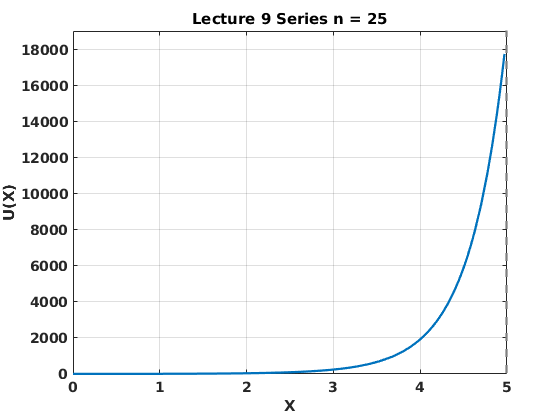
\includegraphics{lec9_fig1.png}
\caption{Power series solution to $u^{\prime \prime}-(1+x)u=0, \ u(0)=5,\ u^{\prime}(0)=1$.}
\label{fig:lec9_fig1}
\end{marginfigure}
\begin{lstlisting}[name=lec9_ex1,style=myMatlab]
xMin = 0; xMax = 5;
figure(1)
fplot(u,[xMin, xMax],'linewidth',2);
title_str = sprintf('Lecture 9 Series n = %d',n);
title(title_str,'fontsize',18,'fontweight','bold');
xlabel('X','fontsize',16,'fontweight','bold');
ylabel('U(X)','fontsize',16,'fontweight','bold');
set(gca,'fontsize',12,'fontweight','bold');
grid on
\end{lstlisting}
\marginnote{\textbf{Note:} Pay particular attention to the formatting details of the plot.  There is a title along with axis-labels for both the x- and y-axis; fonts are bold and sized in a systematic way.  Grid lines are also used to make the graph more readable.  These details have all been added in observance of MATLAB Style Rule \#4. 

The variables \lstinline[style=myMatlab]{xMin} and \lstinline[style=myMatlab]{xMax} on line 39 has been included in accordance with Rule \#8.  The fact that both variables are initialized on the same line is a common exception to Rule \#9.}
\newthought{A few more} details are worth noting.  
\begin{enumerate}
\item We know our solution is inexact since we truncated the infinite power series and used finite-precision arithmetic while calculating the coefficients for those terms we \emph{did} bother to include.  Still, we might want to know \emph{how wrong} the solution is.
\item Taking a more positive tack, we might ask how much \emph{better} the solution gets when we add more terms to our solution.
\end{enumerate}
To answer either of these questions, we will need access to the solution of the IVP.  For this lecture, we will take a numeric solution generated using MATLAB's built-in IVP-solving tool \emph{ODE45} as ``the solution.''\marginnote[-1.0cm]{Use of tools such as \emph{ODE45} will be treated in the numerical methods section.}
\begin{marginfigure}
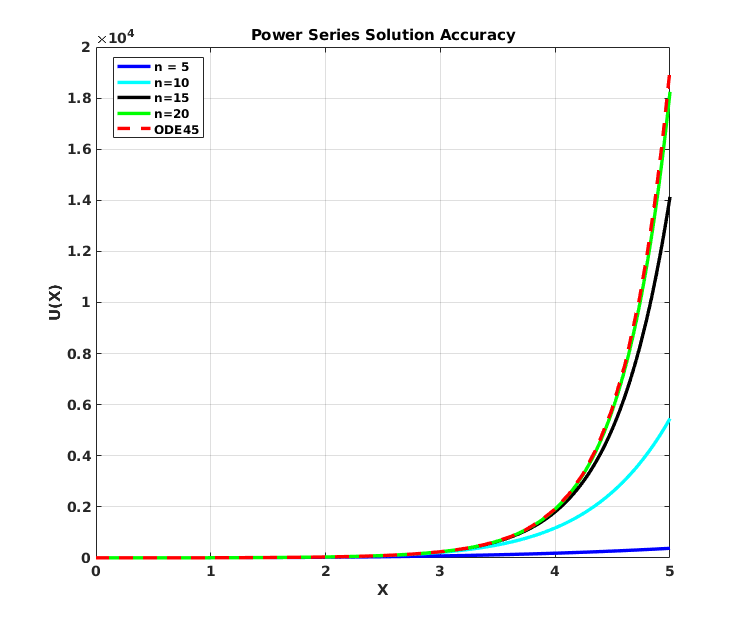
\includegraphics{lec9_ps_compare.png}
\caption{Power series solution with different values of $n$.}
\label{fig:lec9_ps_compare}
\end{marginfigure}

Power series results for various values of $n$ are compared to the numerical solution in Figure \ref{fig:lec9_ps_compare}.  Some things to notice:
\begin{enumerate}
\item The solution gets worse the further one gets from zero; and
\item The solution gets better for larger values of $n$.  
\end{enumerate}
Neither of these observations should be surprising but there is value to seeing it in your results. It adds confidence to the proposition that your (approximate) solution is correct.

\newthought{As a last note} it should be pointed out that, while plots like that shown in Figure \ref{fig:lec9_ps_compare} gives a good qualitative feel for how the solution is improving as the number of power series terms increases, a quantitative measure for correctness is preferable.  In Figure \ref{fig:lec9_ps_converge} a quantitative measure---the relative error in the 2-norm---is used to quantify the difference between different power series solutions and the solution generated using \emph{ODE45}.  Details of this error measure will be discussed in future lectures.
\begin{marginfigure}
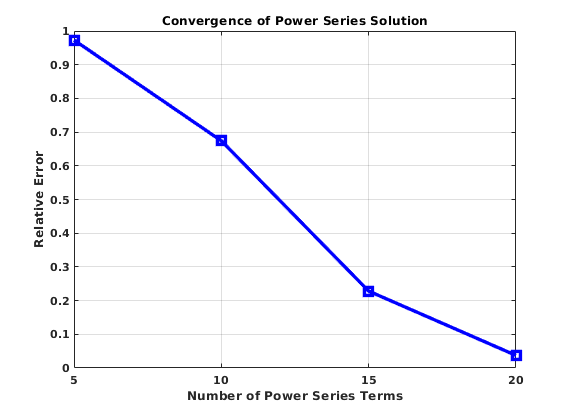
\includegraphics{lec9_ps_converge.png}
\caption{Convergence of the power series solution to the numeric solution.}
\label{fig:lec9_ps_converge}
\end{marginfigure}   


\chapter{Lecture 10 - Legendre's Equation}
\label{ch:lec10}
\section{Objectives}
The objectives of this lecture are:
\begin{itemize}
\item Illustrate the use of the power series method to solve Legendre's equation. 
\item Introduce some of the properties of Legendre polynomials.
\end{itemize}

\section{Legendre's Equation}
The following 2\textsuperscript{nd}-order linear, homogeneous ODE is known as Legendre's equation:
\begin{equation}
\left(1-x^2 \right)u^{\prime \prime}-2xu^{\prime} + m(m+1)u = 0 
\label{eq:legendre}
\end{equation}
where $m$ is a constant.

\newthought{First we will} put Equation \ref{eq:legendre} into standard form:
\begin{equation*}
u^{\prime \prime} - \frac{2x}{\left( 1-x^2 \right)}u^{\prime} + \frac{m(m+1)}{\left(1-x^2 \right)}u = 0
\end{equation*}
We should immediately note that $P(x) = \frac{2x}{\left( 1-x^2 \right)}$ and $Q(x) = \frac{m(m+1)}{\left(1-x^2 \right)}$ are singular (and thus not analytic) at $x=\pm1$. Recall from Theorem \ref{thm:existence-of-power-series-solutions} that $P(x)$ and $Q(x)$ must be analytic for power series solutions to exist.
\newthought{We will restrict} our attention to the interval $x \in (-1,1)$ and use the power series method to find a solution.  Inserting our assumed power series solution into Equation \ref{eq:legendre} gives us:
\begin{fullwidth}
\begin{align*}
\left(1-x^2 \right)\sum\limits_{n=2}^{\infty} n(n-1)c_nx^{n-2} - 2x\sum\limits_{n=1}^{\infty} n c_nx^{n-1} + m(m+1)\sum\limits_{n=0}^{\infty}c_nx^n & = 0 \\
\underbrace{\sum\limits_{n=2}^{\infty}n(n-1)c_nx^{n-2}}_{x^0} - \underbrace{\sum\limits_{n=2}^{\infty}n(n-1)c_nx^n}_{x^2} - \underbrace{\sum\limits_{j=1}^{\infty}2nc_nx^n}_{x^1} + \underbrace{m(m+1)\sum\limits_{n=0}^{\infty}c_nx^n}_{x^0} &= 0
\end{align*}
\end{fullwidth}
where we see that all terms with order lower than $x^2$ need to be pulled outside of their summations so all four can be in phase.
\begin{fullwidth}
\begin{multline*}
(2)(1)c_2 + (3)(2)c_3x + \underbrace{\sum\limits_{n=4}^{\infty}n(n-1)c_nx^{n-2}}_{\substack{k=n-2 \\ n=k+2}} - \underbrace{\sum\limits_{n=2}^{\infty}n(n-1)c_nx^{n}}_{\substack{k=n \\ n=k}} - (2)(1)c_1x - \underbrace{\sum\limits_{n=2}^{\infty}2nc_nx^n}_{\substack{k=n \\ n=k}} + \dots \\
m(m+1) \left(c_0 + c_1x\right) + m(m+1)\underbrace{\sum\limits_{n=2}^{\infty}c_n x^n}_{\substack{k=n \\ n=k}} = 0
\end{multline*}
Combining terms outside of the summations and making the indicated substitutions to combine the summations we get:
\begin{multline*}
\left[m(m+1)c_0 + 2c_2 \right] + [\underbrace{(m(m+1)-2)}_{(m-1)(m+2)}c_1 + 6c_3]x + \dots \\
\sum\limits_{k=2}^{\infty}[(k+2)(k+1)c_{k+2} \underbrace{- k(k-1)c_k - 2kc_k + m(m+1)c_k}_{(m-k)(m+k+1)c_k}]x^k = 0
\end{multline*}
\end{fullwidth}
Applying the indicated algebraic simplifications leads us finally to:\marginnote{\textbf{Note:} Obviously this is a tedious business.  Be careful and make sure you understand each manipulation.}
\begin{multline*}
[m(m+1)c_0+2c_2] + [(m+1)(m+2)c_1 + 6c_3]x + \cdots \\
\sum\limits_{k=2}^{\infty}[(k+2)(k+1)c_{k+2} + (m-k)(m+k+1)c_k]x^k=0
\end{multline*}
The next steps are to find formulas for the power series coefficients, $c_n$, so that the combined coefficient for each power of $x$ in the equation above equals zero. For the constant term $(x^0)$ we have:
\begin{equation*}
c_2 = \frac{-m(m+1)c_0}{2}
\end{equation*}
For the linear term $(x^1)$ we get:
\begin{equation*}
c_3 = \frac{-(m-1)(m+2)}{6}c_1
\end{equation*}
For all other powers of $x$, we get a 2-term recurrence:
\begin{equation*}
c_{k+1} = \frac{-(m-k)(m+k+1)}{(k+2)(k+1)}c_k
\end{equation*}
\begin{margintable}
\begin{tabular}{l}
$k=2$ \\
$c_4 = \frac{-(m-2)(m+3)}{(4)(3)}c_2 = \frac{(m-2)(m+3)m(m+1)}{(4)(3)(2)}c_0$ \\
$k=3$ \\
$c_5 = \frac{-(m-3)(m+4)}{(5)(4)}c_3 = \frac{(m-3)(m+4)(m-1)(m+2)}{(5)(4)(3)(2)}c_1$ \\
\end{tabular}
\end{margintable}
\noindent Organizing these into two solutions we get:
\begin{align*}
u_1(x) &= c_0\left[1 + \frac{c_2}{c_0}x^2 + \frac{c_4}{c_0}x^4 + \cdots \right] \\
&= c_0 \left[1-\frac{m(m+1)}{2!}x^2 + \frac{(m-2)(m+3)m(m+1)}{4!}x^4 + \cdots  \right] \\
u_2(x) &= c_1\left[x + \frac{c_3}{c_1}x^3 + \frac{c_5}{c_1}x^5 + \cdots \right] \\
&= c_1\left[x - \frac{(m-1)(m+2)}{3!}x^3+\frac{(m-3)(m+4)(m-1)(m+2)}{5!}x^5 + \cdots \right]
\end{align*}
So far what we have is messy but, when dealing with power series solutions, messiness is the order of the day.  One point that we have quietly left to the side is whether or not we expect this (so called) power series solution  to converge.\marginnote{\textbf{Reminder:} If the power series that we purport to be a solution to the differential equation is divergent than we really have nothing.}

One way that we can permanently leave these questions to the side is if $m$ is an integer.  Notice that if $m=0$ or is an even integer,\sidenote{i.e. If $m$ is even then $u_1(x)$ is a polynomial.} $u_1(x)$ terminates with a finite number of terms. Similarly with $u_2(x)$ in the case that $m$ is an odd integer. 

\newthought{These polynomial solutions}, where $m$ is an integer, are referred to as Legendre polynomials.  Legendre polynomials have several important applications; our primary use for them will be when solving equations in spherical coordinate systems.

\section{Important Properties of Legendre Polynomials}
Legendre polynomials are solutions to Legendre's equation where $m$ is an integer:
\begin{equation*}
\left(1-x^2 \right)u^{\prime \prime} - 2xu^{\prime} + m(m+1)u = 0
\end{equation*}

By convention the leading coefficients are chosen such that Legendre polynomials have a maximum value of 1 on the interval $x\in[-1,1]$.  

\begin{margintable}
\begin{tabular}{c | c}
$P_0(x) = 1$ & $P_1(x) = x$ \\\hline
$P_2(x) = \frac{1}{2}(3x^2-1)$ & $P_3(x) = \frac{1}{2}(5x^3-3x)$ \\
\end{tabular}
\caption{The first four Legendre Polynomials}
\label{tab:Legendre-poly}
\end{margintable}
The first few Legendre Polynomials are shown in the Table \ref{tab:Legendre-poly}. Higher order Legendre polynomials can be constructed using a three-term recurrence relation shown in Equation \ref{eq:legendre-three-term}:
\begin{equation}
(n+1)P_{n+1}(x) - (2n+1)xP_n(x) + nP_{n-1}(x) = 0
\label{eq:legendre-three-term}
\end{equation}

\vspace{4.0cm}

Some other properties include:

\begin{align*}
P_n(-x) &= (-1)^nP_n(x) \\
P_n(1) &= 1 \\
P_n(-1) &= (-1)^n \\
P_n(0) &= 0 \text{ for } n\in{\text{odd}} \\
P_n^{\prime}(0) &=0 \text{ for } n\in{\text{even}}
\end{align*}
\begin{marginfigure}
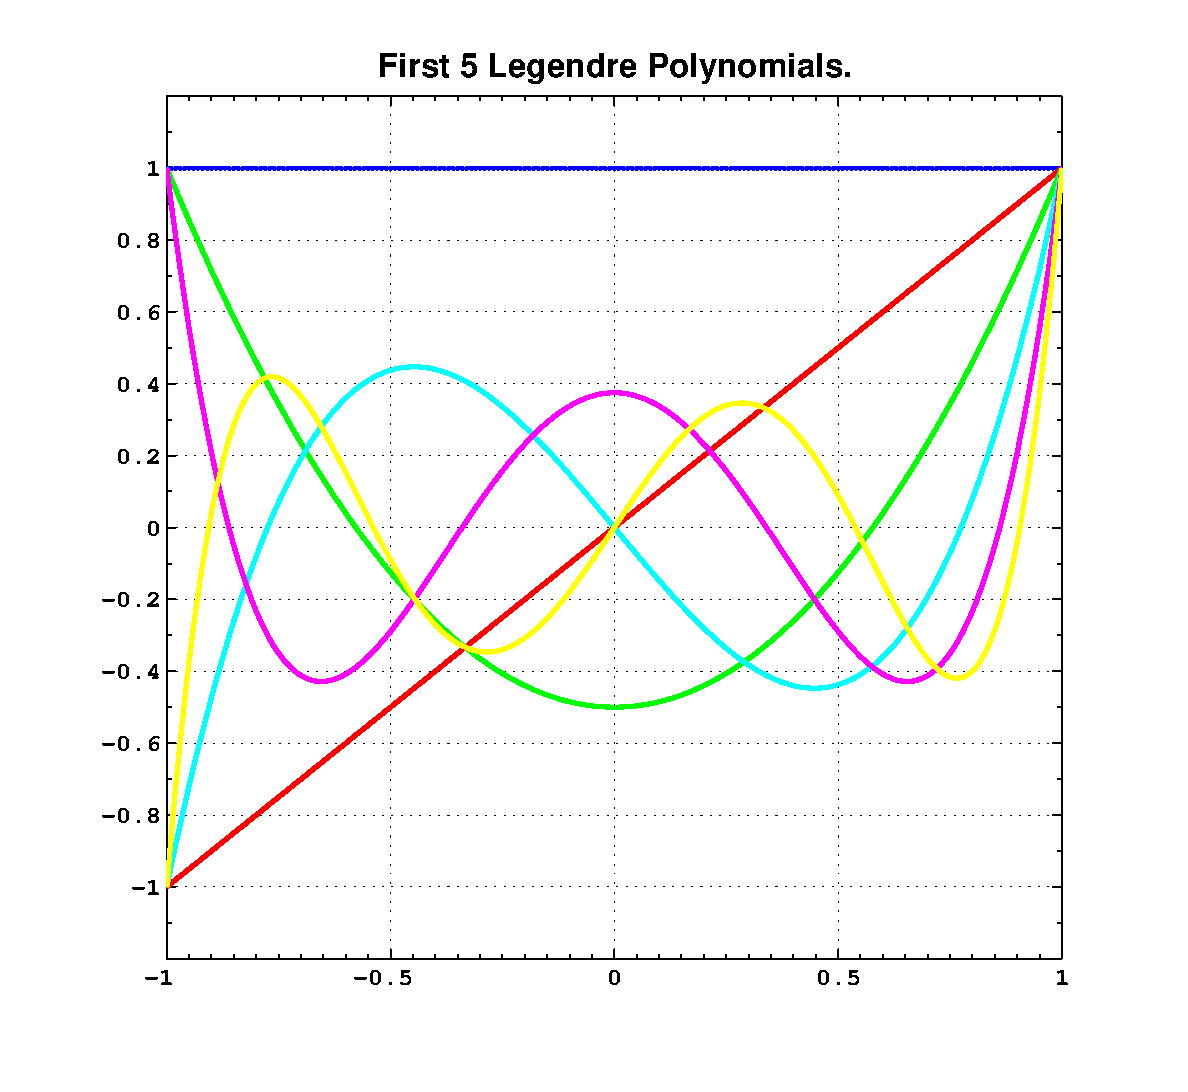
\includegraphics{LegendrePolyPlot.eps}
\caption{Legendre Polynomials of order 0 through 5.}
\label{fig:legendre-poly-plot}
\end{marginfigure}
A plot of the first few Legendre Polynomials is shown in Figure \ref{fig:legendre-poly-plot}.


\newthought{The last property} that we will mention here, and that we will make use of extensively in this course, is the \emph{orthogonality} property of Legendre polynomials.\marginnote[1.0cm]{Orthogonality of functions is analogous to orthogonality of vectors.  Two functions, $f_1(x)$ and $f_2(x)$ are orthogonal on an interval $x\in[a,b]$ if $\int_a^b f_1(x)f_2(x) \ dx = 0$.}
Legendre polynomials are orthogonal over the interval $x \in [-1,1]$.  This mean that Equation \ref{eq:legendre-orthogonality} holds:
\begin{equation}
\int_{-1}^{1} P_n(x) P_m(x) \ dx = 
\begin{cases}
0, \ \ n \ne m \\
\frac{2}{n+1}, \ \ n = m \\
\end{cases}
\label{eq:legendre-orthogonality}
\end{equation}


\chapter{Lecture 11 - Solutions about Singular Points}
\label{ch:lec11}
\section{Objectives}
The objectives of this lecture are:
\begin{itemize}
\item Define regular and irregular singular points and give examples of their classification.
\item Describe the extended power series method (method of Frobenius).
\item Do an example problem.
\end{itemize}

\section{Definitions}
Consider a linear, homogeneous, second-order differential equation in standard form as shown below:
\begin{equation*}
u^{\prime \prime} + P(x)u^{\prime} + Q(x)u = 0
\end{equation*}

\begin{definition}[Singular Point]
A \emph{singular point}, $x_0$, is a point where $P(x)$ or $Q(x)$ are not analytic.
\end{definition}

\begin{definition}[Regular/Irregular Singular Point]
A singular point $x_0$ is said to be a \emph{regular} singular point of the differential equation if the functions $p(x)=(x-x_0)P(x)$ and $q(x)=(x-x_0)^2Q(x)$ are both analytic at $x_0$.  If a singular point is not regular, it is \emph{irregular}.
\end{definition}

\noindent\textbf{Example:} Classify the singular points of $(x^2-4)^2u^{\prime\prime}+3(x-2)u^{\prime}+5u = 0$.

\vspace{0.5cm}

\noindent In standard form, $P(x) = \frac{3(x-2)}{(x^2-4)^2} = \frac{3(x-2)}{(x+2)^2(x-2)^2}$; and $Q(x) = \frac{5}{(x+2)^2(x-2)^2}$.  There are two singular points: -2 and 2.\marginnote[-1.0cm]{\underline{$x_0=2$}:$\ \ \ p(x) = \frac{\cancel{(x-2)}3\cancel{(x-2)}}{(x+2)^2 \cancel{(x-2)^2}}$, so $p(x) = \frac{3}{(x+2)^2}$ which is analytic at $x=2$. $q(x) = \frac{\cancel{(x-2)^2} 5}{(x+2)^2\cancel{(x-2)^2}}$, so $q(x) = \frac{5}{(x+2)^2}$ which is analytic at $x=2$.

\vspace{0.3cm}

\underline{$x_0=-2$}:$ \ \ p(x) = \frac{(x+2)3(x-2)}{(x+2)^2(x-2)^2}$ so $p(x) = \frac{3(x-2)}{(x+2)(x-2)}$ which is \underline{not} analytic at $x=-2$.  $q(x)=\frac{\cancel{(x+2)^2} 5}{\cancel{(x+2)^2}(x-2)^2}$, so $q(x) = \frac{5}{(x-2)^2}$ which is analytic at $x=-2$.}
Work is shown in the margin for $p(x)$ and $q(x)$.  From the work in the margin it should be clear for this problem that $q(x)$ is analytic at both $x=-2$ and $x=2$ but, since $p(x)$ is not analytic at $x_0=-2$, $x_0=-2$ is an irregular singular point; $x_0=2$ is a regular singular point.

\begin{theorem}[Frobenius' Theorem]
If $x=x_0$ is a \emph{regular} singular point then there exists at least one non-zero solution of the form:
$$u(x) = (x-x_0)^r\sum\limits_{n=0}^{\infty}c_n(x-x_0)^n = \sum\limits_{n=0}^{\infty}c_n(x-x_0)^{n+r}$$
where $r$ is to be determined.  The series will converge at least on some radius of convergence defined by: $0<x-x_0<R$.
\label{thm:frobenius}
\end{theorem}

%\vspace{0.5cm} 
\section{Method of Frobenius}
The definitions and theorems provided above lead us to the method of Frobenius which we will illustrate through example.

\vspace{0.25cm}

\noindent\textbf{Example:} Find a series solution to: $3xu^{\prime \prime} + u^{\prime} - u = 0$.\marginnote{You should verify that this equation has a regular singluar point at $x_0=0$.}

\noindent Per Theorem \ref{thm:frobenius}, this equation should have a solution of the form: $u = \sum_{n=0}^{\infty}c_nx^{n+r}$ where $r$ is constant. Taking the first and second derivatives we get:\marginnote{Notice in this case that the summations for $u^{\prime}$ and $u^{\prime \prime}$ start at $n=0$ while for the power series solution method the starting index for $u^{\prime}$ was $n=1$ and the starting index for $u^{\prime \prime}$ was $n=2$.  

The reason for this is that, for the power series method, the constant term of $u$, corresponding to $n=0$, becomes zero for $u^{\prime}$; so we omit that term and start with $n=1$.  Both the constant and linear term in $u$, corresponding to $n=0$ and $n=1$, are zero for $u^{\prime \prime}$.  So the series for $u^{\prime \prime}$ starts at $n=2$.

The factor $x^r$ included in the method of Frobenius means there may not be any constant terms in the series at all---i.e. if $r$ is not an integer.  Therefore there is no reason to omit terms for $u^{\prime}$ or $u^{\prime \prime}$.}
\begin{align*}
u^{\prime} &= \sum\limits_{n=0}^{\infty}(n+r)c_nx^{n+r-1} \\
u^{\prime\prime} &= \sum\limits_{n=0}^{\infty}(n+r)(n+r-1)c_nx^{n+r-2}
\end{align*}

\noindent We insert these expressions into the differential equation and will combine the summations to derive recurrence relations.

%\begin{fullwidth}
\begin{align*}
3x\sum\limits_{n=0}^{\infty}(n+r)(n+r-1)c_nx^{n+r-2} + \sum\limits_{n=0}^{\infty}(n+r)c_nx^{n+r-1} - \sum\limits_{n=0}^{\infty}c_nx^{n+r} &= 0 \\
\sum\limits_{n=0}^{\infty}3(n+r)(n+r-1)c_nx^{n+r-1} + \sum\limits_{n=0}^{\infty}(n+r)c_nx^{n+r-1} - \sum\limits_{n=0}^{\infty}c_nx^{n+r} &= 0 \\
\end{align*}
%\end{fullwidth}
\begin{align*}
x^r\left[\underbrace{\sum\limits_{n=0}^{\infty}3(n+r)(n+r-1)c_nx^{n-1}}_{\substack{\text{for }n=0 \\ x^{-1}}} + \underbrace{\sum\limits_{n=0}^{\infty}(n+r)c_nx^{n-1}}_{\substack{\text{for }n=0 \\ x^{-1}}} - \underbrace{\sum\limits_{n=0}^{\infty}c_nx^n}_{\substack{\text{for }n=0 \\ x^{0}}} \right] &= 0 \\
\end{align*}

%\vspace{2.0cm}

\noindent We can see now that one term must be ``peeled off'' from the first two summations in order to get the summations in phase. 


\begin{multline}
x^r \left[\sum\limits_{n=1}^{\infty} 3(n+r)(n+r-1)c_nx^{n-1} + \sum\limits_{n=1}^{\infty} (n+r)c_nx^{n-1} - \sum\limits_{n=0}^{\infty}c_nx^n \right] + \cdots \\
\underbrace{x^r\left[3r(r-1) + r \right]c_ox^{-1}}_{\substack{\text{first terms from} \\ \text{first two summations}}} = 0
\label{eq:lec11_ex1_e1}
\end{multline}
Let us focus for a moment on the last term on the left-hand side of Equation \ref{eq:lec11_ex1_e1}.\marginnote{$x^{r}\left[3r(r-1)+r \right]c_ox^{-1}=0$

\vspace{0.5cm}

\noindent\textbf{Option \#1} set $c_0 = 0$; 

\vspace{0.25cm}

\noindent\textbf{Option \#2} set $r$ to a root of $3r(r-1)+r = 0$.}  We know from our experience with the power series solution process that, in order to \emph{solve} the equation, the coefficient for each power of $x$ needs to be zero.  Consider now specifically the coefficient for $x^{r-1}$.  That coefficient needs to be zero and there are a couple of ways that it can be set to zero which are discussed in the margin note.

\index{method of Frobenius}
\newthought{The customary procedure} for the method of Frobenius dictates that we go with option \#2.  We refer to---$3r(r-1)+r = 0$---as the \emph{indicial equation} and the roots of the indicial equation are known as the \emph{indicial roots.}\sidenote[][-0.5cm]{For second-order problems, the form of the indicial equation will be a quadratic.} 

\newthought{For this case,} the indicial equation can be factored:
\begin{align*}
f(x) &= 3r(r-1)+r \\
&=3r^2-3r+r \\
&=3r^2-2r \\
&=r(3r-2) = 0
\end{align*}
so the roots are $r_1=0$, and $r_2 = \sfrac{2}{3}$. So long as $r$ is chosen to be one of those values, the coefficient for $x^{r-1}$ will be zero.  Let us refocus our attention on the remaining terms:

\begin{equation*}
x^r \left[\sum\limits_{n=1}^{\infty} 3(n+r)(n+r-1)c_nx^{n-1} + \sum\limits_{n=1}^{\infty} (n+r)c_nx^{n-1} - \sum\limits_{n=0}^{\infty}c_nx^n \right] = 0
\end{equation*}
The summations are all in phase---recall that is how we obtained the indicial equation---but we need to combine the three summations under a common index.
\begin{equation*}
x^r \left[\underbrace{\sum\limits_{n=1}^{\infty} 3(n+r)(n+r-1)c_nx^{n-1}}_{\substack{k=n-1 \\ n=k+1}} + \underbrace{\sum\limits_{n=1}^{\infty} (n+r)c_nx^{n-1}}_{\substack{k=n-1 \\ n=k+1}} - \underbrace{\sum\limits_{n=0}^{\infty}c_nx^n}_{\substack{k=n \\n=k}} \right] = 0
\end{equation*}
Making the indicated substitution in each summation gives us:
\begin{equation*}
x^r\left\{\sum\limits_{k=0}^{\infty} \underbrace{\left[\underbrace{3(k+1+r)(k+r)c_{k+1}+(k+1+r)c_{k+1}}_{(k+1+r)(3(k+r)+1)c_{k+1}} - c_k\right]}_{(k+1+r)(3(k+r)+1)c_{k+1} - c_k = 0}x^k\right\} = 0
\end{equation*}
The resulting recurrence relation for the coefficient of $x^{k+r}$ is:
\begin{equation*}
c_{k+1}=\frac{c_k}{(k+1+r)(3k+3r+1)}
\end{equation*}
We have two cases: one for $r=0$; the other for $r = \sfrac{2}{3}$.

\vspace{0.25cm}
\noindent\underline{$r=0$}:
\begin{equation*}
c_{k+1} = \frac{c_k}{(k+1)(3k+1)}
\end{equation*}
\noindent Coefficients are shown in the table in the margin; the resulting solution is:
\begin{margintable}
\begin{tabular}{|l|} 
\hline
\textbf{case 1, } $\mathbf{r = 0}$ \\\hline
$k = 0$ \\
$c_1 = \frac{c_0}{(1)(1)} = c_0$ \\\hline
$k = 1$ \\
$c_2 = \frac{c_1}{(2)(4)} = \frac{c_0}{8}$ \\\hline
$k=2$ \\
$c_3 = \frac{c_2}{(3)(7)} = \frac{c_0}{(3)(7)(8)}$\\\hline
\end{tabular}
\end{margintable}

\begin{align*}
u_1(x) &= x^0\left(c_0 + c_1x + c_2x^2 + c_3x^3 + \cdots \right) \\
&= c_0\left(1 + \frac{c_1}{c_0}x + \frac{c_2}{c_0}x^2 + \frac{c_3}{c_0}x^3 + \cdots \right) \\
&= c_0\left(1+x+\frac{1}{8}x^2+\frac{1}{168}x^3+\cdots \right)
\end{align*}
\vspace{0.25cm}
\noindent\underline{$r=\sfrac{2}{3}$}:
\begin{align*}
c_{k+1} &=\frac{c_k}{(k+1+\frac{2}{3})(3k+3\left(\frac{2}{3}\right)+1)}\\
&=\frac{c_k}{\left(k+\frac{5}{3}\right)(3k+3)} \\
&=\frac{c_k}{(3k+5)(k+1)}
\end{align*}
\noindent Coefficients are shown in the table in the margin; the resulting solution is:
\begin{margintable}
\begin{tabular}{|l|}
\hline
\textbf{case 2, } $\mathbf{r=\sfrac{2}{3}}$ \\\hline
$k=0$ \\
$c_1 = \frac{c_0}{(5)(1)} = \frac{c_0}{5}$ \\\hline
$k=1$ \\
$c_2 = \frac{c_1}{(8)(2)} = \frac{c_0}{(2)(5)(8)}$ \\\hline
$k=2$ \\
$c_3 = \frac{c_2}{(11)(3)} = \frac{c_0}{(2)(3)(5)(8)(11)}$\\\hline
\end{tabular}
\end{margintable}
\begin{align*}
u_2(x) &= x^{\sfrac{2}{3}}\left(c_0 + c_1x + c_2x^2 + c_3x^3 + \cdots \right) \\
&= c_0x^{\sfrac{2}{3}}\left(1 + \frac{c_1}{c_0}x+\frac{c_2}{c_0}x^2+\frac{c_3}{c_0}x^3 + \cdots \right) \\
&= c_0x^{\sfrac{2}{3}}\left(1+\frac{1}{5}x + \frac{1}{80}x^2+\frac{1}{264}x^3 + \cdots  \right)
\end{align*}

\newthought{A quick inspection} of $u_1(x)$ and $u_2(x)$ should be sufficient to convince you that the solutions are linearly independent.  The general solution to the differential equation comprises a linear combination of $u_1(x)$ and $u_2(x)$.

%\vspace{5.0cm}

\section{Indicial Equation} \index{indicial equation}
It turns out that we could have determined the indicial roots before setting out upon the method of Frobenius.  Recall that we use the method of Frobenius on differential equations with regular singular points; also recall that a regular singular point is one where $p(x)=xP(x)$ and $q(x)=x^2Q(x)$ are both analytic.  By definition, if $p(x)$ and $q(x)$ are analytic, that means that they can be represented as a convergent power series.  Suppose we did that, and expressed $p(x)$ and $q(x)$ as a power series; if we did they could be written as:
\begin{align*}
p(x) &= \sum\limits_{n=0}^{\infty} a_nx^n = a_0 + a_1x + a_2x^2 + \cdots \\
q(x) &= \sum\limits_{n=0}^{\infty} b_nx^n = b_0 + b_1x + b_2x^2 + \cdots
\end{align*}
It can be shown that the indicial equation that we derive from the Method of Frobenius will be equal to:
\begin{equation*}
r(r-1)+a_0r + b_0 = 0
\end{equation*}
where $a_0 = p(0)$ and $b_0 = q(0)$.  Applying this equation to our last example where $p(x)=xP(x) = \sfrac{1}{3}$ and $q(x) = x^2 Q(x) = -\sfrac{x}{3}$.  We can see $a_0 = p(0) = \sfrac{1}{3}$ and $b_0 = q(0) = 0$.  Inserting these numbers into the indicial equation gives us:
\begin{align*}
r(r-1)+\frac{1}{3}r + 0 &= 0 \\
r^2-r + \frac{1}{3}r &= 0 \\
r^2 - \frac{2}{3}r &= 0 \\
r(r-\frac{2}{3}) &=0
\end{align*}
which has the roots: $r = 0$, and $r = \sfrac{2}{3}$.

\vspace{0.5cm}

\noindent\textbf{Example:}  Use the indicial equation to determine the indicial roots to:
\begin{equation*}
2xu^{\prime \prime} - (3+2x)u^{\prime} + u = 0
\end{equation*}

\vspace{0.25cm}

\noindent We see that $P(x) = -\frac{(3 - 2x)}{2x}$, so $p(x) = xP(x) = -\frac{(3-2x)}{2}$, and $p(0) = -\sfrac{3}{2}$.  By inspection $q(x) = x^2Q(x) = \frac{x}{2}$, so $q(0) = 0$.  The indicial equation is:
\begin{align*}
r(r-1)-\frac{3}{2}r + 0 &= 0 \\
r^2-r - \frac{3}{2}r &= 0 \\
r^2 - \frac{5}{2}r &= 0 \\
r\left(r-\frac{5}{2}\right) &= 0
\end{align*}
so the indicial roots are: $r = 0$, and $r = \sfrac{5}{2}$.


\newthought{In general, of course,} the indicial equation is just a quadratic equation, so the roots may be real and repeated, real and distinct or complex conjugates.  There are three cases that will be of immediate interest to us:
\begin{enumerate}
\item Two distinct real roots that do \emph{not} differ by an integer.  In this case it can be shown that there exist two linearly independent solutions: $u_1 = \sum_{n=0}^{\infty}c_nx^{n+r_1}$, and $u_2 = \sum_{n=0}^{\infty}c_nx^{n+r_2}$.\marginnote{In both of these cases we implicitly assume that $c_0 \ne 0$.}
\item Two distinct real roots that differ by an integer.  In this case there exist two linearly independent solutions of the form:
\begin{align*}
u_1(x) &= \sum\limits_{n=0}^{\infty}c_nx^{n+r_1}, \ \ c_0 \ne 0 \\
u_2(x) &= C u_1(x) \ln{x} + \sum\limits_{n=0}^{\infty}b_nx^{n+r_2}, \ \ b_0 \ne 0 
\end{align*}
In this case, the constant $C$ \emph{might} be zero.
\item If both roots are real and $r_1 = r_2$ then there exist two linearly independent solutions of the form:
\begin{align*}
u_1(x) &= \sum\limits_{n=0}^{\infty}c_nx^{n+r_1}, \ \ c_0 \ne 0 \\
u_2(x) &= u_1(x) \ln{x} + \sum\limits_{n=0}^{\infty}b_nx^{n+r_2}, \ \ b_0 \ne 0
\end{align*}
\end{enumerate}
\marginnote[-6.0cm]{\textbf{Note:} The goal in this treatment of method of Frobenius is not to make you a ``Frobenius Genius.''  The goal is to provide a sufficiently thorough introduction so that you can understand where Bessel functions and other such mathematical objects come from.  For this reason, we will emphasize systems that fall into case 1.}

\noindent Additional Notes:

\begin{itemize}
\item When the difference between the indicial roots is equal to an integer, find the solution with the smaller root first.

\item The indicial equation could, in principle, have complex roots.  We will avoid those cases for this class.

\item If $x_0$ is an irregular singular point, the Frobenius theorem does not apply and we may not be able to find any solution to the differential equation using this method.
\end{itemize}\marginnote[-2.0cm]{For ordinary differential equations that fall into the last two categories, do not fret: numerical methods are always available that are more than adequate for finding solutions to the equations.}

\chapter{Assignment \#4}
\label{ch:ass4}
\begin{fullwidth}
Find two power series solutions of the given differential equation.
\begin{enumerate}
\item $u^{\prime \prime} + x^2 u^{\prime} + xu = 0$

\vspace{1.0cm}

\item $u^{\prime \prime} - (x+1)u^{\prime} - u = 0$
\end{enumerate}

\vspace{1.0cm}



\begin{enumerate}[resume]
\item Solve the given initial value problem.  Use MATLAB to represent the power series.  Make 2 plots; for the first plot compare the partial sum of the power series with 5 terms to the exact solution which is $u=8x-2e^x$; for the second plot compare the partial sum of the power series with 15 terms to the exact solution.  Submit the ``published'' version of your MATLAB script (PDF format) along with your written solution.

\begin{equation*}
(x-1)u^{\prime \prime} - xu^{\prime} + u = 0, \ \ u(0)=-2, \ u^{\prime}(0) = 6
\end{equation*}
\end{enumerate}

\vspace{1.0cm}

\noindent Determine the singular points for the differential equation.  Classify each singular point as irregular or regular.
\begin{enumerate}[resume]
\item $\left(x^2-9 \right)^2u^{\prime \prime} + (x+3)u^{\prime} + 2u = 0$

\vspace{1.0cm}

\item $x^3\left(x^2 - 25\right)\left(x-2\right)^2u{\prime \prime}+3x(x-2)u^{\prime}+7(x+5)u = 0$
\end{enumerate}

\vspace{1.0cm}

\noindent Use the general form of the indicial equation to find the indicial roots.

\begin{enumerate}[resume]
\item $x^2u^{\prime \prime} + \left(\frac{5}{3}x+x^2 \right)u^{\prime}-\frac{1}{3}u = 0$
\end{enumerate}

\vspace{1.0cm}

\noindent Use the method of Frobenius to obtain two linearly independent series solutions:
\begin{enumerate}[resume]
\item $3xu^{\prime \prime} + (2-x)u^{\prime} - u = 0$
\end{enumerate}

\end{fullwidth}

\chapter{Lecture 12 - Bessel's Equation and Bessel Functions}
\label{ch:lec12}
\section{Objectives}
The objectives of this lecture are:
\begin{itemize}
\item Introduce Bessel's equation and solve it using the method of Frobenius.
\item Discuss Bessel functions of the 1\textsuperscript{st} and 2\textsuperscript{nd} kind and use them to solve instances of Bessel's equation.
\end{itemize}

\section{Bessel's Equation}

Bessel's equation is given in Equation \ref{eq:bessels}:
\index{Bessel's Equation}
\begin{equation}
x^{2}u^{\prime \prime} + x u^{\prime} + \left(x^2 - \nu^2\right)u = 0
\label{eq:bessels}
\end{equation}
where $\nu$ is a constant.\sidenote{Let me warn you for the first time here that, if $\nu=0$, Bessel's equation bears a striking resemblance to the Cauchy-Euler equation.  Notice the difference and try not to fall into that trap.}  You should spend a moment to verify that this equation has a singular point at $x_0 = 0$ and that it is a regular singular point.  Therefore we should use the method of Frobenius to find solutions and that is what we shall do.

\newthought{As a reminder}, we will make the following substitutions into Equation \ref{eq:bessels}:
\begin{align*}
u(x) &= \sum\limits_{n=0}^{\infty}c_n x^{n+r} \\
u^{\prime}(x) &= \sum\limits_{n=0}^{\infty} (n+r)c_nx^{n+r-1} \\
u^{\prime \prime}(x) &= \sum\limits_{n=0}^{\infty}(n+r)(n+r-1)c_nx^{n+r-2}
\end{align*}
which gives us:
%\begin{fullwidth}
\begin{equation*}
x^2\sum\limits_{n=0}^{\infty}(n+r)(n+r-1)c_nx^{n+r-2} + x\sum\limits_{n=0}^{\infty}(n+r)c_nx^{n+r-1} + \left(x^2-\nu^2 \right)\sum\limits_{n=0}^{\infty}c_nx^{n+r} = 0 
\end{equation*}
\noindent or, if we distribute terms through the sums:
\begin{equation*}
\sum\limits_{n=0}^{\infty}(n+r)(n+r-1)c_nx^{n+r} + \sum\limits_{n=0}^{\infty}(n+r)c_nx^{n+r} + \sum\limits_{n=0}^{\infty}c_nx^{n+r+2} - \sum\limits_{n=0}^{\infty}\nu^2c_nx^{n+r} = 0 
\end{equation*}

%\end{fullwidth}
Let us inspect the first term in each summation and see what needs to be done to get the summations in phase.
%\begin{fullwidth}
\begin{equation*}
\underbrace{\sum\limits_{n=0}^{\infty}(n+r)(n+r-1)c_nx^{n+r}}_{n=0, \ x^r} + \underbrace{\sum\limits_{n=0}^{\infty}(n+r)c_nx^{n+r}}_{n=0, \ x^r} + \underbrace{\sum\limits_{n=0}^{\infty}c_nx^{n+r+2}}_{n=0, \ x^{r+2}} - \underbrace{\sum\limits_{n=0}^{\infty}\nu^2c_n x^{n+r}}_{n=0, \ x^r} = 0
\end{equation*}
%\end{fullwidth}
For reasons that (hopefully) will become apparent, we are going to go through this process in two steps.  For $n=0$, we will separate out all terms that are proportional to $x^r$.
%\begin{fullwidth}
\begin{multline*}
r(r-1)c_0x^r + x^r\sum\limits_{n=1}^{\infty}(n+r)(n+r-1)c_nx^n + rc_0x^r + x^r\sum\limits_{n=1}^{\infty}(n+r)c_nx^n + \cdots \\
x^r\sum\limits_{n=0}^{\infty}c_nx^{n+2} - \nu^2c_0x^r - x^r\sum\limits_{n=1}^{\infty}\nu^2c_nx^{n} = 0
\end{multline*}
%\end{fullwidth}
Now let us collect the terms outside of the summations and re-write the equation:\marginnote{The first line of the equation is the indicial equation for this problem; we use it to determine allowable values of $\nu$.  In the second line of the equation we have combined the first, second, and fourth summation because they were in phase and had a common index.  The remaining summation needs to be put in phase before we can combine everything under a single summation.}
\begin{multline*}
\overbrace{\left[r(r-1)+r - \nu^2 \right]}^{\text{indicial equation}}c_ox^r + \cdots \\ x^r\sum\limits_{n=1}^{\infty}\underbrace{\left[(n+r)(n+r-1) + (n+r) - \nu^2\right]}_{\text{combined 3 of 4 summations}}c_nx^n +  x^r\sum\limits_{n=0}^{\infty}c_nx^{n+2} = 0
\end{multline*}
From the indicial equation:
\begin{align*}
r(r-1)+r-\nu^2 &= 0\\
r^2 - r + r - \nu^2 &= 0 \\
r^2 - \nu^2 &= 0 \\
(r - \nu)(r+\nu) &= 0
\end{align*}
we see that, to ensure the coefficient for $x^r = 0$, $r = \pm \nu$.\marginnote[-2.5cm]{\textbf{Reminder:} We need to ensure the coefficient for $x^r$ is equal to zero.  By convention we assume $c_0 \ne 0.$  We \emph{could} allow $c_0 = 0$ but then we would just need to derive another indicial equation for some other power of $x$.  We adopt the convention $c_0 \ne 0$ so that our choices for indicial roots will be unique.}
To simplify the discussion to follow, let us take $r = \nu$ and continue with the solution.  Our equation is now: 
\begin{align*}
x^{\nu}\sum\limits_{n=1}^{\infty}\left[\underbrace{(n+\nu)(n+\nu-1) + (n+\nu)-\nu^2}_{n^2+2n\nu+\nu^2 - \nu^2} \right]c_nx^n + x^{\nu}\sum\limits_{n=0}^{\infty}c_n x^{n+2} &= 0 \\
x^{\nu}\sum\limits_{n=1}^{\infty} \underbrace{\left[n(n+2\nu) \right]c_nx^n}_{n=1, \ x^1} + x^{\nu}\sum\limits_{n=0}^{\infty}\underbrace{c_nx^{n+2}}_{n=0, \ x^2} &= 0
\end{align*}
The two summations are out of phase, so we need to separate out the first term of the first summation.
\begin{equation*}
\underbrace{(1)(1+2\nu)c_1}_{\text{coefficient for }x^{\nu+1}}x^{\nu+1} + \underbrace{x^{\nu}\sum\limits_{n=2}^{\infty}c_n[n(n+2\nu)]x^n}_{n=2, \ x^{\nu+2}} + \underbrace{x^{\nu}\sum\limits_{n=0}^{\infty}c_nx^{n+2}}_{n=0, \ x^{\nu+2}} = 0
\end{equation*}
In order to satisfy the equation, we need the coefficient for $x^{\nu+1}$ to be equal to zero; the only way to do this is to set $c_1 = 0$.\sidenote{Remember: we do not control what $\nu$ is; that is part of the equation.}

The summations in the equation above are in-phase so we need to combine under a common index. 
\begin{align*}
x^{\nu}\underbrace{\sum\limits_{n=2}^{\infty}c_n[n(n+2\nu)]x^n}_{\substack{k=n \\ n=k}} + x^{\nu}\underbrace{\sum\limits_{n=0}^{\infty}c_nx^{n+2}}_{\substack{k=n+2 \\ n=k-2}} &= 0 \\
x^{\nu}\sum\limits_{k=2}^{\infty}\underbrace{\left[k(k+2\nu)c_k + c_{k-2}\right]}_{\text{coefficient for } x^{\nu+k}}x^{k} &= 0
\end{align*}
In order to set the coefficients for $x^{\nu+k}$ to zero, we derive the following two-term recurrence:
\begin{equation}
c_k = \frac{-c_{k-2}}{k(k+2\nu)} \ , \ \ k=2,3,4,\dots
\label{eq:bessel-recurrance}
\end{equation}
Since we have already determined that $c_1=0$, Equation \ref{eq:bessel-recurrance} tells us that $c_3=c_5=\cdots=0$; all the odd-numbered coefficients must be zero. To simplify the notation further, we will thus assume that $k=2n$ and re-write our recurrence as:
\begin{align*}
c_{2n} &= \frac{-c_{2n-2}}{2n(2n+2\nu)} \ , \ \ n=1,2,3,\dots \\
&=\frac{-c_{2n-2}}{2^2n(n+\nu)} \ , \ \ n=1,2,3,\dots
\end{align*}
\begin{margintable}
\begin{tabular}{|l|}
\hline
$n=1$ \\
$c_2 = \frac{-c_0}{2^2(1)(1+\nu)}$ \\\hline
$n=2$ \\
$c_4 = \frac{-c_2}{2^2 (2)(2+\nu)} = \frac{c_0}{2^4(1)(2)(1+\nu)(2+\nu)}$\\\hline
$n=3$ \\
$c_6 = \frac{-c_4}{2^2 (3)(3+\nu)} = \frac{-c_0}{2^6(1)(2)(3)(1+\nu)(2+\nu)(3+\nu)}$ \\\hline
\end{tabular}
\caption{First few coefficients in solution to Bessel's Equation.}
\label{tab:bessel-coef}
\end{margintable}
\noindent Expressions for the first few terms is given in Table \ref{tab:bessel-coef}. From this pattern you should be able to see that the general form of the coefficients is as shown in Equation \ref{eq:bessel-coef}.
\begin{equation}
c_{2n} = \frac{(-1)^n c_0}{2^{2n}n!(1+\nu)(2+\nu)\cdots(n+\nu)} \ , \ \ n=1,2,3,\dots
\label{eq:bessel-coef}
\end{equation}
\newthought{It may be worthwhile} to take a step back and summarize what we have found so far.  We are solving Bessel's equation; we looked for solutions of the form $u(x)=\sum_{n=0}^{\infty} c_n x^{n+r}$.  We found that $r$ must be equal to $\pm \nu$ and, for the case $r = \nu$, derived a perfectly acceptable expression for the coefficients in this solution in Equation \ref{eq:bessel-coef}.\marginnote{We will deal with the case $r = -\nu$, albeit in a perfunctory manner, below.} What follows is a bit of, what we will call, ``mathematical grooming'' which we will do so that we can derive solutions to Bessel's equation in a form that appears elsewhere in the literature and that, it turns out, you will use for the remainder of this course.
\subsection{Gamma Function}\index{Gamma function}
The gamma function is defined in Equation \ref{eq:gamma-def}.
\begin{equation}
\Gamma(x) = \int_0^{\infty} t^{x-1}e^{-t} \ dt
\label{eq:gamma-def}
\end{equation}
One property of the gamma function is that $\Gamma(x+1) = x \Gamma(x)$ for any real argument $x$.\marginnote{\textbf{Note:} The gamma function is also defined when a complex argument is used, but that is beyond the scope of this class.} If $x$ is an integer, this makes the gamma function equivalent to a factorial: 
\begin{align*}
\Gamma(1) &= \int_0^{\infty}t^{1-1} e^{-t} \ dt \\
&= \int_0^{\infty}e^{-t} \ dt \\
&= -e^{-t}\Bigr|_0^{\infty} \\
&= -[0 - 1] \\
&= 1
\end{align*}
\marginnote{Put differently, the Gamma function is a \emph{generalization} of a factorial.}
\begin{align*}
\Gamma(2) &= \Gamma(1+1) = 1\Gamma(1) = 1 \\
\Gamma(3) &= \Gamma(2+1) = 2\Gamma(2) = 2 \\
\Gamma(4) &= \Gamma(3+1) = 3\Gamma(3) = 6 \\
\end{align*}
In general for $x \in \mathcal{I}$, $\Gamma(x) = (x-1)!$. 

\newthought{In the context} of our solution to Bessel's equation, we use the gamma function to compactly represent the term $(1+\nu)(2+\nu)\cdots(n+\nu)$ in the denominator of Equation \ref{eq:bessel-coef}:
\begin{align*}
\Gamma(1+\nu+1) &= (1+\nu)\Gamma(1+\nu) \\
\Gamma(1+\nu+2) &= (2+\nu)\Gamma(2+\nu) = (2+\nu)(1+\nu)\Gamma(1+\nu) \\
\Gamma(1+\nu+3) &= (3+\nu)\Gamma(3+\nu) = (3+\nu)(2+\nu)(1+\nu)\Gamma(1+\nu) \\
\vdots \\
\Gamma(1+\nu+n) &= (n+\nu)\cdots(1+\nu)\Gamma(1+\nu)
\end{align*}

\subsection{Bessel Function of the First Kind of order $\nu$}
We will use everything that we have done thus far to define a Bessel function of the first kind of order $\nu$.  We will start with our series solution $u(x) = \sum_{n=0}^{\infty}c_n{x^{n+\nu}}$ and the formula for the non-zero (even) coefficients given in Equation \ref{eq:bessel-coef} and take a couple of steps:
\begin{enumerate}
\item We will set $c_0 = \frac{1}{2^{\nu}\Gamma(1+\nu)}$.\marginnote{Remember $c_0$ is just an arbitrary constant.  This decision allows us, with the help of gamma functions, to express the coefficients to the solution in a compact form.  The resulting solution can then be multiplied by \emph{another} arbitrary constant if needed to satisfy a given initial/boundary condition.}
\begin{align*}
c_{2n} &= \frac{(-1)^n c_0}{2^{2n}n!(1+\nu)(2+\nu)\cdots(n+\nu)}, \ \ n=1,2,3,\dots \\
&= \frac{(-1)^n}{2^{2n}n!(1+\nu)(2+\nu)\cdots(n+\nu)}\frac{1}{2^{\nu}\Gamma(1+\nu)} \\
&= \frac{(-1)^n}{2^{2n+\nu}n!(1+\nu)\cdots(n+\nu)\Gamma(1+\nu)} \\
&= \frac{(-1)^n}{2^{2n+\nu}n!\Gamma(1+\nu+n)}
\end{align*}  
\item Combining this new expression for $c_{2n}$ into the solution gives us the standard definition for a Bessel function of the first kind:
\begin{equation}
J_{\nu}(x) = \sum\limits_{n=0}^{\infty}\frac{(-1)^n}{n!\Gamma(1+\nu+n)}\left(\frac{x}{2}\right)^{2n+\nu}
\label{eq:beq-first-kind-order-nu}
\end{equation}\marginnote[-1.0cm]{It can be shown that if $\nu \ge 0$ the series converges for all $x$.}\marginnote{We were sly about it, but we quietly added the $n=0$ term to the summation.  A more verbose expression would be:
\begin{align*}
u(x) &= c_0x^0 + \sum_{n=1}^{\infty}c_{2n}x^{2n+\nu} \\
&= \frac{1}{2^{\nu}\Gamma(1+\nu)} + \sum_{n=1}^{\infty}\frac{(-1)^n}{2^{2n+\nu}n!\Gamma(1+\nu+n)}x^{2n+\nu} \\
&= \frac{1}{2^{2(0)+\nu}0!\Gamma(1+\nu+0)} + \cdots \\
& \cdots \sum_{n=1}^{\infty}\frac{(-1)^n}{2^{2n+\nu}n!\Gamma(1+\nu+n)}x^{2n+\nu} \\
&= \sum\limits_{n=0}^{\infty}\frac{(-1)^n}{2^{2n+\nu}n!\Gamma(1+\nu+n)}x^{2n+\nu} \\
&= \sum\limits_{n=0}^{\infty}\frac{(-1)^n}{n!\Gamma(1+\nu+n)}\left(\frac{x}{2}\right)^{2n+\nu}
\end{align*}
}
We can similarly handle the case where $r = -\nu$:
\begin{equation*}
J_{-\nu} = \sum\limits_{n=0}^{\infty}\frac{(-1)^n}{n!\Gamma(1-\nu+n)}\left(\frac{x}{2} \right)^{2n-\nu}
\end{equation*}

\end{enumerate}
We will not prove this, but if $\nu$ is \emph{not} an integer, then $J_{\nu}$ and $J_{-\nu}$ are linearly independent. In that case, the solution (at long last) to Bessel's equation is just a linear combination of $J_{\nu}(x)$ and $J_{-\nu}(x)$ as shown in Equation \ref{eq:beq-sol}.
\begin{equation}
u(x) = c_1J_{\nu}(x) + c_2J_{-\nu}(x)
\label{eq:beq-sol}
\end{equation}

\subsection{Bessel Function of the Second Kind of order $\nu$}
If $\nu$ is an integer, then $J_{\nu}(x)$ and $J_{-\nu}(x)$ are \emph{\underline{not}} linearly independent so we need to find another solution to Bessel's equation.  To this end, we define the Bessel function of the second kind of order $\nu$, given in Equation \ref{eq:beq-second-kind}:
\begin{equation}
Y_{\nu}(x) = \frac{\cos{\nu \pi} J_{\nu}(x) - J_{-\nu}(x)}{\sin{\nu \pi}}
\label{eq:beq-second-kind}
\end{equation}
which is linearly independent of $J_{\nu}$ even if $\nu$ is an integer.  The solution to Bessel's equation can thus alternately be expressed:\marginnote{I recommend that you always use $J_{\nu}$ and $Y_{\nu}$.  It's not hard to decide if $\nu$ is an integer or not but consistency has its benefits.}
\begin{equation*}
u(x) = c_1J_{\nu}(x) + c_2Y_{\nu}(x)
\end{equation*}

\newthought{Now that we know} a pair of linearly independent solutions to Bessel's equation, we no longer need to go through the rigmarole of \emph{actually solving} the equation; we can simply \emph{\underline{use}} the solution we have derived.

\vspace{1.0cm}

\noindent\textbf{Example:} Find the general solution to:
\begin{equation*}
x^2u^{\prime \prime} + xu^{\prime} + \left(x^2 - \frac{1}{9} \right)u = 0
\end{equation*}
We recognize the given equation as Bessel's equation of order $\nu = \sfrac{1}{3}$.  Therefore the general solution is: 
\begin{equation*}
u(x) = c_1J_{\sfrac{1}{3}}(x) + c_2Y_{\sfrac{1}{3}}(x)
\end{equation*}
Alternatively we could, of course, have used: $u(x) = c_1J_{\sfrac{1}{3}}(x) + c_2J_{-\sfrac{1}{3}}(x)$.

\vspace{1.0cm}

\noindent\textbf{Example:} Find the general solution to:
\begin{equation*}
xu^{\prime \prime} + u^{\prime} + xu = 0
\end{equation*}
To the uninitiated this may not look like Bessel's equation but with practice you will learn to automatically see the above equation as: 
\begin{align*}
xu^{\prime \prime} + u^{\prime} + xu &= 0, \ \ \text{ multiply by x} \\
x^2u^{\prime \prime} + xu^{\prime} + x^2u &= 0 \\
x^2u^{\prime \prime} + xu^{\prime} + \left(x^2-0^2\right)u &= 0
\end{align*}
and recognize it to be Bessel's equation of order zero.  The general solution is:
\begin{equation*}
u(x) = c_1J_0(x) + c_2Y_0(x)
\end{equation*}

\chapter{Lecture 13 - Solving ODEs Reducible to Bessel's Equation}
\label{ch:lec13}
\section{Objectives}
Demonstrate reducing and ODE to Bessel's Equation by:
\begin{itemize}
\item changing the dependent variable;
\item changing the independent variable; and
\item changing both the dependent and independent variables.
\end{itemize}

\newthought{If we have learned} one thing over the course of the last couple of lectures it is that using the method of Frobenius---whether we are solving Bessel's equation or some other differential equation with regular singular points---is tedious and error-prone.  The good news is that if we are trying to solve a problem and recognize that the problem is Bessel's equation of some order, we can simply write down the solution in terms of Bessel functions.\sidenote{Let me reiterate that this was \underline{the point} to learning how to solve Bessel's equation.}  Of course, if the equation is \emph{not} Bessel's equation, this ability offers little benefit.

In this and the next lecture we will learn some techniques by which a broad range of differential equations can be transformed into or expressed as Bessel's equation, thereby expanding the range of equations for which we may write the soluton in terms of Bessel functions.  The best way to learn is by doing, so we will simply start with the examples.

\vspace{0.5cm}

\noindent\textbf{Example:} Find the general solution to the following differential equation by applying the given transformation to the dependent variable: $u = \sfrac{v}{x^2}$.\marginnote{You can think of this as cleverly distorting the $y$-axis in order to make the problem easier.}
\begin{equation*}
xu^{\prime \prime} + 5u^{\prime} + xu = 0
\end{equation*}

\vspace{4.0cm}

We need to replace all appearances of $u$ with the equivalent in terms of $v$.\marginnote{
Using the product rule:
\begin{align*}
u &= \frac{v}{x^2} \\
u^{\prime} &= \frac{-2v}{x^3} + \frac{v^{\prime}}{x^2} \\
u^{\prime \prime} &= \frac{6v}{x^4} \underbracket{-\frac{2v^{\prime}}{x^3}-\frac{2v^{\prime}}{x^2}}_{\frac{-4v^{\prime}}{x^3}} + \frac{v^{\prime \prime}}{x^2}
\end{align*}
where $\sfrac{dv}{dx} = v^{\prime}$.
}
\begin{align*}
xu^{\prime \prime} &= \frac{v^{\prime \prime}}{x} - \frac{4v^{\prime}}{x^2} + \frac{6v}{x^3} \\
5u^{\prime} &= \frac{5v^{\prime}}{x^2} - \frac{10v}{x^{3}} \\
xu &= \frac{v}{x}
\end{align*}

Combining these terms together gives us:\marginnote[1.0cm]{Seeing the necessary transformations comes with practice; that is what homework is for.}
\begin{align*}
xu^{\prime \prime} + 5u^{\prime} + xu &= 0 \\
\frac{v^{\prime \prime}}{x} - \frac{4v^{\prime}}{x^2} + \frac{6v}{x^3} + \frac{5v^{\prime}}{x^2} - \frac{10v}{x^{3}} + \frac{v}{x} &= 0, \ \ \text{ combine like terms}\\
\frac{v^{\prime \prime}}{x}+\frac{v^{\prime}}{x^2} + \left(\frac{1}{x}-\frac{4}{x^3} \right)v &= 0, \ \ \ \text{multiply by }x^3 \\
x^2v^{\prime \prime} + xv^{\prime} + \left(x^2 - 4 \right)v &= 0
\end{align*}
where on the last line we recognize the ODE as Bessel's equation of order $\nu = 2$.  The solution is:
\begin{equation*}
v(x) = c_1J_2(x) + c_2Y_2(x)
\end{equation*}
Of course, we were trying to solve for $u(x)$ so we must undo the transformation to the dependent variable:
\begin{equation*}
u(x) = \frac{v(x)}{x^2} = \frac{1}{x^2}\left[ c_1J_2(x) + c_2Y_2(x)\right]
\end{equation*}

\vspace{1.0cm}

\noindent\textbf{Example:} Find the general solution to the following differential equation by applying the given transformation to the independent variable: $\sqrt{x} = z$.\marginnote{This is like cleverly distorting the $x$-axis with the goal of making the problem easier.}
\begin{equation*}
4xu^{\prime \prime} + 4u^{\prime} + u = 0
\end{equation*}
In this case we need to change occurrences of $x$ into its equivalent in terms of $z$ and we need to change all derivatives with respect to $x$ to derivatives with respect to $z$.  We are given $\sqrt{x}=z$ which is, of course, equivalent to $x = z^2$.  For the derivatives we have:\marginnote{\textbf{Note:} It is important that you purge all expressions including $x$ out of these derivatives.  For example, when computing the equivalent of $u^{\prime}$ it was essential that we make the substitution $x^{-\sfrac{1}{2}} = z^{-1}$.  When we used that result in calculating $u^{\prime \prime}$ and took derivatives with respect to $z$, any occurrence of $x$ needed to be replaced with its equivalent in $z$ or the derivative would have been wrong.}
\begin{align*}
u^{\prime} &= \frac{du}{dx} = \frac{du}{dz}\frac{dz}{dx} = u_z\frac{d}{dx}\left(x^{\sfrac{1}{2}}\right) = \frac{1}{2}\underbracket{x^{-\sfrac{1}{2}}}_{z^{-1}}u_z  \\
&=\frac{1}{2z}u_z \\
u^{\prime \prime} &= \frac{d}{dx}\left(\frac{du}{dx} \right) = \frac{d}{dz}\left(\frac{du}{dx}\right)\frac{dz}{dx} \\
&=\frac{d}{dz}\left[\frac{1}{2z}u_z\right]\frac{1}{2z} = \left[-\frac{1}{2z^2}u_z + \frac{1}{2z}u_{zz} \right] \frac{1}{2z} \\
&=\frac{1}{4z^2}u_{zz}-\frac{1}{4z^3}u_z
\end{align*}
We now substitute these results into the original equation:
\begin{align*}
4xu^{\prime \prime} &= 4z^2\left[\frac{1}{4z^2}u_{zz}-\frac{1}{4z^3}u_z \right] \\
4u^{\prime} &= 4\left[\frac{1}{2z}u_z\right]
\end{align*}
So the transformed equation is:
\begin{align*}
u_{zz}-\frac{1}{z}u_z + \frac{2}{z}u_z + u &= 0, \ \ \ \text{ combine like terms}\\
u_{zz} + \frac{1}{z}u_z + u &= 0, \ \ \ \text{ multiply by }z^2 \\
z^2u_{zz} + zu_{z} + \underbracket{z^2}_{\left(z^2-0^2\right)}u &= 0
\end{align*}
and we can immediately recognize this as Bessel's equation of order $\nu = 0$. The general solution is:
\begin{align*}
u(z) &= c_1J_0(z) + c_2Y_0(z), \ \ \ \text{ undo transformation: }z\to x \\
u(x) &= c_1J_0(\sqrt{x}) + c_2Y_0(\sqrt{x})
\end{align*}

\vspace{1.0cm}

\noindent\textbf{Example: }Find the general solution to the equation below by transforming the dependent variable $u = v\sqrt{x}$, and the independent variable $\sqrt{x} = z$.\marginnote{In this case we are distorting \emph{both} the $x$- and $y$-axis to ``simplify'' the problem.}

\begin{equation*}
x^2u^{\prime \prime}+\frac{1}{4}\left(x+\frac{3}{4}\right)u = 0
\end{equation*}
\noindent We will first transform the dependent variable: $u=v\sqrt{x} = x^{\sfrac{1}{2}}v$.  As before we will replace all appearances of $u$ with the equivalent in terms of $v$.  Using the product rule:
\begin{align*}
u &= x^{\sfrac{1}{2}}v \\
u^{\prime} &= \frac{1}{2}x^{-\sfrac{1}{2}}v + x^{\sfrac{1}{2}}v^{\prime} \\
u^{\prime \prime} &= -\frac{1}{4}x^{-\sfrac{3}{2}}v+\underbracket{\frac{1}{2}x^{-\sfrac{1}{2}}v^{\prime} + \frac{1}{2}x^{-\sfrac{1}{2}}v^{\prime}}_{x^{-\sfrac{1}{2}}v^{\prime}}+x^{\sfrac{1}{2}}v^{\prime \prime}
\end{align*}
and inserting into our equation gives us:
\begin{equation*}
x^2\left[x^{\sfrac{1}{2}}v^{\prime \prime}+x^{-\sfrac{1}{2}}v^{\prime}-\frac{1}{4}x^{-\sfrac{3}{2}}v \right] + \frac{1}{4}\left[x+\frac{3}{4}\right]x^{\sfrac{1}{2}}v = 0
\end{equation*}
Now we transform the independent variable $\sqrt{x} = z$, which is the same transformation that we did for the last example so we will not repeat the work.\marginnote[-1.5cm]{From the last example:
\begin{align*}
v^{\prime} &= \frac{1}{2z}v_z \\
v^{\prime \prime} &= \frac{1}{4z^2}v_{zz} - \frac{1}{4z^3}v_z 
\end{align*}
} 

\noindent Inserting these expressions for $v^{\prime}$ and $v^{\prime \prime}$ into the equation and if we also add the following identities: $x^{\sfrac{1}{2}}=z, \ x=z^2, \ \text{and }x^2=z^4$ we get: 

\begin{multline*}
z^4\left[ z\left(\frac{1}{4z^2}v_{zz}-\frac{1}{4z^3}v_z\right) + \frac{1}{z}\left(\frac{1}{2z}v_z \right)-\frac{1}{4}z^{-3}v\right]+ \cdots \\
\cdots \frac{1}{4}\left(z^3+\frac{3}{4}\right)zv = 0 
\end{multline*}
Distributing the $z$'s and grouping terms gives us:
\begin{align*}
\frac{z^3}{4}v_{zz}+\left(-\frac{z^2}{4}+\frac{z^2}{2} \right)v_z + \left(-\frac{z}{4}+\frac{z^3}{4}+\frac{3z}{16}\right)v &= 0, \text{ combining like terms}\\
\frac{z^3}{4}v_{zz}+\frac{z^2}{4}v_z + \left(\frac{z^3}{4}-\frac{z}{16} \right) &= 0, \ \text{ multiply by }\sfrac{4}{z} \\
z^2v_{zz}+zv_z+\left(z^2-\frac{1}{4}\right)v &= 0
\end{align*}
which, at long last, we recognize as Bessel's equation of order $\nu = \sfrac{1}{2}$.  The solution, by inspection, is:
\begin{align*}
v(z) &= c_1J_{\sfrac{1}{2}}(z) + c_2 Y_{\sfrac{1}{2}}(z), \ \ \text{un-transform the dependent variable.} \\
u(z) &= \sqrt{x}\left(c_1J_{\sfrac{1}{2}}(z) + c_2 Y_{\sfrac{1}{2}}(z) \right), \ \ \text{un-transform the independent variable.} \\
u(x) &= \sqrt{x}\left(c_1J_{\sfrac{1}{2}}(\sqrt{x}) + c_2Y_{\sfrac{1}{2}}(\sqrt{x})\right)
\end{align*}

\vspace{1.0cm}

\noindent\textbf{Notes:}
\begin{itemize}
\item Obviously, one would need to have spectacular insight to know in advance what transformations should be made in order to convert a given differential equation into Bessel's equation.  
\item In the next lecture we will make use of some tools that have been developed to simplify these transformations.
\end{itemize}


\chapter{Lecture 14 - Modified Bessel Function and Parametric Modified Bessel Function}
\label{ch:lec14}
\section{Objectives}
\begin{itemize}
\item Show how to use the parametric Bessel equation of order $\nu$.
\item Describe the modified Bessel equation and, their solutions, modified Bessel functions.
\item Introduce and illustrate a tool for solving second-order ODEs in terms of Bessel functions.
\end{itemize}

Many differential equations can be solved in terms of Bessel functions.  This lecture will introduce some relatively simple and powerful tools for doing so.

\section{Parametric Bessel Equation of Order $\nu$}
The parametric Bessel equation of order $\nu$ has the form given in Equation \ref{eq:pbe-form}:

\begin{equation}
x^{2}u^{\prime \prime} + xu^{\prime} + \left(\alpha^2 x^2 - \nu^2 \right)u= 0
\label{eq:pbe-form}
\end{equation}

Rather than state the solution outright, let us take a different shortcut and apply the well-known transformation that will convert Equation \ref{eq:pbe-form} into Bessel's equation that we can solve, by inspection, with Bessel functions.

\newthought{The transformation is} $t = \alpha x$.  This, of course, means that $x = \sfrac{t}{\alpha}$ and the derivatives of $u$ with respect to $t$ are shown in the margin.\marginnote{The derivatives of $u$ with respect to $t$:
\begin{align*}
\frac{dt}{dx} &= \alpha \\
u^{\prime} &= \frac{du}{dx} = \frac{du}{dt}\frac{dt}{dx} = \alpha u_t \\
u^{\prime \prime} &= \frac{d}{dx}\left(\frac{du}{dx}\right) = \cdots \\
&= \frac{d}{dt}\left(\frac{du}{dx}\right)\frac{dt}{dx} = \cdots \\
&=\frac{d}{dt}\left(\alpha u_t\right)\alpha = \alpha^{2}u_{tt}
\end{align*}
} Applying these substitutions gives us:
\begin{align*}
x^{2}u^{\prime \prime} + xu^{\prime} + \left(\alpha^2 x^2 - \nu^2 \right)u &= 0 \\
\frac{t^2}{\alpha^2}\alpha^2 u_{tt} + \frac{t}{\alpha}\alpha u_t + \left(\alpha^2 \frac{t^2}{\alpha^2} - \nu^2 \right)u &= 0 \\
t^2u_{tt} + t u_{t} + \left(t^2 - \nu^2\right)u &= 0
\end{align*}
The last line is, of course, Bessel's equation and the solution is:\marginnote{At this point in the course you should be developing a list, of sorts, of differential equations that you recognize and know how to analyze.  Call it something like: \emph{``A Field Guide to Differential Equations I Know How To Solve''.}  This list should include:
\begin{itemize}
\item first-order linear equations
\item separable equations
\item linear constant-coefficient equations
\item linear equations with variable coefficients, including:
\begin{itemize}
\item Cauchy-Euler equations
\item Legendre's equation
\item Bessel's equation; and now
\item parametric Bessel's equation.
\end{itemize}

\end{itemize} 
For these last problem types you ``solve'' them by recognizing the equation and writing down the solution.} 
\begin{equation*}
u(t) = c_1J_{\nu}(t) + c_2Y_{\nu}(t)
\end{equation*}
Undoing the change of independent variables to express the answer in terms of $x$ gives us the solution shown in Equation \ref{eq:pbe-sol}.
\begin{equation}
u(x) = c_1J_{\nu}(\alpha x) + c_2Y_{\nu}(\alpha x)
\label{eq:pbe-sol}
\end{equation}

\vspace{0.5cm}

\noindent\textbf{Example:} Use the parametric Bessel equation to find the general solution to:
\begin{equation*}
x^2u^{\prime \prime} + xu^{\prime} + \left(36x^2 - \frac{1}{4} \right)u = 0
\end{equation*}
We recognize the equation as a parametric Bessel equation; the parameter $\alpha = \sqrt{36} = 6$ and $\nu^2 = \sfrac{1}{4} \Rightarrow \nu = \sfrac{1}{2}$.  The solution is:\marginnote{\textbf{Note: }for the example, instead of using $Y_{\sfrac{1}{2}}(6x)$ as the second linearly independent solution, we could have used $J_{-\sfrac{1}{2}}(6x)$; it is entirely up to you.}
\begin{equation*}
u(x) = c_1 J_{\sfrac{1}{2}}(6x) + c_2Y_{\sfrac{1}{2}}(6x)
\end{equation*}

\section{Modified Bessel Equations and Bessel Functions}
A subtle but non-trivial variation to Bessel's equation is when we flip one crucial sign as shown in Equation \ref{eq:mbeq-form}:
\begin{equation}
x^2u^{\prime \prime} + xu^{\prime}-\left(x^2 + \nu^2\right)u = 0
\label{eq:mbeq-form}
\end{equation}
\index{Bessel's Equation, parametric}
\index{Bessel's Equation, modified}
\index{Bessel Function, modified}
This equation can be converted into Bessel's equation by transforming the dependent variable---$u=i^{-\nu}v$---and independent variable---$t=ix$.  We will omit these details and instead simply give the solution as shown in Equation \ref{eq:mbeq-solution} which includes modified Bessel functions of the first\sidenote{Modified Bessel functions of the first kind are defined as:
\begin{equation*}
I_{\nu}(x) = i^{-\nu}J_{\nu}(ix)
\end{equation*}} and second kind\sidenote{Modified Bessel functions of the second kind, analogous to Bessel functions of the second kind, are defined in terms of modified Bessel functions of the first kind:
\begin{equation*}
K_{\nu}(x) = \frac{\pi}{2}\frac{I_{\nu}(x)-I_{\nu}(x)}{\sin{\nu \pi}}
\end{equation*}
}:

\begin{equation}
u(x) = c_1I_{\nu}(x) + c_2K_{\nu}(x)
\label{eq:mbeq-solution}
\end{equation}

The modified Bessel's equation also has a parametric form as shown in Equation \ref{eq:mpbeq-form}:
\begin{equation}
x^2u^{\prime \prime} + xu^{\prime} - \left(\alpha^2 x^2 + \nu^2 \right)u = 0
\label{eq:mpbeq-form}
\end{equation}
with the general solution given in Equation \ref{eq:mpbeq-solution}.
\begin{equation}
u(x) = c_1I_{\nu}(\alpha x) + c_2 K_{\nu}(\alpha x)
\label{eq:mpbeq-solution}
\end{equation}

\vspace{5.0cm}

\section{Tool for Solving Second-Order ODEs}
A more general-purpose tool for solving linear, homogeneous, second-order ODEs in terms of Bessel functions is presented in Zill\cite{zill2020advanced} and shown below in Equation \ref{eq:bessel-tool}.

\begin{equation}
u^{\prime \prime} + \frac{1-2a}{x}u^{\prime} + \left(b^2 c^2 x^{2c-2} + \frac{a^2-p^2c^2}{x^2} \right)u = 0, \ \ p \ge 0
\label{eq:bessel-tool}
\end{equation}
The general solution for equations of this form is given in Equation \ref{eq:bessel-tool-sol}.
\begin{equation}
u = x^a\left[c_1 J_{p}\left(bx^c \right)+c_2Y_{p}\left(bx^c \right) \right]
\label{eq:bessel-tool-sol}
\end{equation}
Using this tool requires you to solve four non-linear equations as shown below:\marginnote{Probably the most challenging or, at least, error-prone part of this process is writing a given ODE in the form of Equation \ref{eq:bessel-tool}.}
\begin{equation*}
%u^{\prime \prime} + \frac{\overbracket{\fbox{$1-2a$}}^{\textcircled{1}}}{x}u^{\prime} + \left(\underbracket{\fbox{$b^2 c^2$}}_{\textcircled{2}} x^{\overbracket{\fbox{$2c-2$}}^{\textcircled{3}}} + \frac{\overbracket{\fbox{$a^2-p^2c^2$}}^{\textcircled{4}}}{x^2} \right)u = 0, \ \ p \ge 0
u^{\prime \prime} + \frac{\overset{\textcircled{1}}{\fbox{$1-2a$}}}{x}u^{\prime} + \left(\underset{\textcircled{2}}{\fbox{$b^2 c^2$}} x^{\overset{\textcircled{3}}{\fbox{$2c-2$}}} + \frac{\overset{\textcircled{4}}{\fbox{$a^2-p^2c^2$}}}{x^2} \right)u = 0, \ \ p \ge 0
\end{equation*}

%\vspace{0.5cm}

\noindent\textbf{Example:}  Use Equation \ref{eq:bessel-tool} to find the general solution to the following differential equation:
\begin{equation*}
x^2 u^{\prime \prime} + \left(x^2 - 2\right)u = 0
\end{equation*}

Re-writing the equation in the form of Equation \ref{eq:bessel-tool} gives us:
\begin{align*}
x^2 u^{\prime \prime} + \left(x^2 - 2\right)u &= 0 \\
u^{\prime \prime} + \frac{x^2-2}{x^2}u &= 0 \\
u^{\prime \prime} + 0u^{\prime} + \left(1x^0 + \frac{-2}{x^2} \right)u &= 0
\end{align*}

Now we solve the four equations:
\begin{itemize}
\item $\textcircled{1}$  $1-2a = 0 \Rightarrow a = \sfrac{1}{2}$
\item $\textcircled{3}$ $2c-2=0 \Rightarrow c = 1$
\item $\textcircled{2}$ $b^2c^2=1, \ \ b^2(1) = 1, \ \Rightarrow b=1$
\item $\textcircled{4}$ $a^2 - p^2c^2=-2$ 
\begin{align*}
\left(\frac{1}{2} \right)^2 - p^2(1)^2 &=-2 \\
p^2 &= \frac{1}{4} + 2 = \frac{9}{4} \\
\Rightarrow p &= \frac{3}{2}
\end{align*}
\end{itemize}
Using Equation \ref{eq:bessel-tool-sol} the general solution is:
\begin{equation*}
u(x) = x^{\sfrac{1}{2}}\left[c_1 J_{\sfrac{3}{2}}(x) + c_2 Y_{\sfrac{3}{2}}(x) \right]
\end{equation*}



\chapter{Assignment \#5}
\label{ch:ass5}
\begin{fullwidth}
Find the general solution to the following differential equations in terms of Bessel Functions:
\begin{enumerate}
\item $4x^2u^{\prime \prime} + 4xu^{\prime} + \left(4x^2-25 \right)u = 0$

\vspace{1.0cm}

\item $ x^2u{\prime \prime}+xu^{\prime}+\left(9x^2-4\right)u = 0$

\vspace{1.0cm}

\item $x^2u^{\prime \prime}+xu^{\prime}-\left(16x^2+\frac{4}{9}\right)u = 0$
\end{enumerate}

\vspace{1.0cm}

\noindent Use the indicated change of variables to find the general solution of the given differential equation.
\begin{enumerate}[resume]
\item $x^2u^{\prime\prime}+2xu^{\prime}+\alpha^2x^2u = 0, \ \ u = x^{-\sfrac{1}{2}}v(x) $
\end{enumerate}

\vspace{1.0cm}

\noindent Use Equation \ref{eq:bessel-tool} to find the general solution of the following differential equation in terms of Bessel functions.
\begin{enumerate}[resume]
\item $xu^{\prime \prime} + 2u^{\prime} + 4u = 0$
\end{enumerate}

\end{fullwidth}

\chapter{Review Problems \#1}
\label{ch:rev1}
\begin{fullwidth}
Solve the following differential equations:
\begin{enumerate}
\item $6x^2u^{\prime \prime} + 5xu^{\prime} - u  = 0$

\vspace{1.0cm}

\item $x^2u^{\prime \prime} -7xu^{\prime}+12u = 0, \ \ u(0)=0, \ u(1) = 0 $

\vspace{1.0cm}


\end{enumerate}

\noindent Use the method of power series to solve the following initial value problem:
\begin{enumerate}[resume]
\item $u^{\prime \prime} + xu^{\prime} + 2u = 0, \ \ u(0) = 3, \ u^{\prime}(0) = -2$

\vspace{1.0cm}

\end{enumerate}

\vspace{1.0cm}

\noindent Use the method of Frobenius to solve the following differential equation:
\begin{enumerate}[resume]
\item $2xu^{\prime \prime}+u^{\prime} + u = 0$

\vspace{1.0cm}

\end{enumerate}

\noindent Find the general solution of the given differential equation in terms of Bessel functions:

\begin{enumerate}[resume]
\item $4x^2u^{\prime \prime} + 4xu^{\prime} + \left(64x^2-9 \right)u = 0$

\end{enumerate}
\end{fullwidth}


\part{Orthogonal Functions and Fourier Series}
\chapter{Lecture 15 - Introduction to Orthogonal Functions}
\label{ch:lec15}
\section{Objectives}
\begin{itemize}
\item Define orthogonal functions, weighted orthogonality, function norms, and complete sets of orthogonal functions.
\item Provide analogies of these concepts as applied to vectors and functions.
\end{itemize}

\newthought{In previous lectures} we were able to solve some differential equations by representing the solution  in the form of an infinite series.  For second-order, homogeneous, linear, variable coefficient ODEs where $P(x)$ and $Q(x)$ are analytic throughout the domain of interest, we used power series:\marginnote{Recall that ODEs of this type can be expressed in standard form as:
\begin{equation*}
u^{\prime \prime} + P(x)u^{\prime} + Q(x)u = 0
\end{equation*}
}
\begin{equation*}
u(x) = \sum\limits_{n=0}^{\infty}c_nx^n
\end{equation*}
For equations with regular singluar points in the domain of interest, we used the method of Frobenius and expressed the solutions:
\begin{equation*}
u(x) = \sum\limits_{n=0}^{\infty}c_nx^{n+r}
\end{equation*}
It should be stressed that, if you calculate the coefficients $(c_n)$ in exact arithmetic and if you sum \emph{all} of the terms $(n\to \infty)$, the representation is \emph{exact}.  Each term in the series is linearly independent from all other terms, so as we keep adding terms to the representation of $u(x)$, greater accuracy is achieved.  

\newthought{Our next idea} is to generalize this approach by representing our solution, $u(x)$, as a linear combination of \emph{orthogonal functions.}\marginnote{\textbf{Emphasis:} For power series and method of Frobenius, each term in the series is a monomial.  Going forward we will use series solutions where each term is an orthogonal function.}

\section{Inner Product and Orthogonality of Functions}
From previous courses in calculus, you should be familiar with the concept of orthogonality of vectors.  We test for orthogonality by taking the ``dot product'' or \emph{inner product}; if the inner product is equal to zero, the vectors are orthogonal, otherwise they are not.\marginnote{Vector dot/inner product:
\begin{align*}
\left(\vec{a},\vec{b}\right) &= \sum\limits_{i=1}^{n}(a_i)(b_i) \\
\vec{a}\cdot \vec{b} &= a_1b_1 + a_2b_2 + \cdots a_nb_n
\end{align*}
}

Orthogonality can also be defined for functions. Consider two functions $u_1(x)$ and $u_2(x)$ defined on an interval $x\in[a,b]$.  The inner product of $u_1(x)$ and $u_2(x)$ is defined in Equation \ref{eq:fun-inner-product}.
\begin{equation}
\left(u_1,u_2\right) = \int_{a}^{b} \ u_1(x)u_2(x) \ dx
\label{eq:fun-inner-product}
\end{equation}
If $\left(u_1,u_2\right)=0$ then $u_1(x)$ and $u_2(x)$ are said to be \emph{orthogonal} on interval $x\in[a,b]$.

\vspace{0.5cm}

\noindent\textbf{Example:} Show that the functions $u_1(x)=x^2$ and $u_2(x)=x^3$ are orthogonal on the interval $x \in[-1,1]$.

\vspace{0.5cm}

\begin{align*}
\left(u_1,u_2\right) &= \int_{-1}^{1} x^2 x^3 \ dx \\
&= \int_{-1}^1 x^5 \ dx = \frac{1}{6}x^6\Bigr|_{-1}^{1} \\
&=\frac{1}{6} - \frac{1}{6} = 0
\end{align*}

\newthought{A slight generalization} is \emph{weighted} orthogonality, where we apply a \emph{weight function}, $p(x)$, to the inner product:
\begin{equation}
\left(u_1,u_2\right) = \int_a^b \ u_1(x)u_2(x)p(x) \ dx
\label{eq:weighted-inner-product}
\end{equation}
where if $\left(u_1,u_2\right)=0$ then we say $u_1(x)$ and $u_2(x)$ are orthogonal with respect to weight function $p(x)$.

\newthought{We can assemble} a set of orthogonal functions on a specified interval.  If $\left\{ \phi_1,\phi_2,\phi_3,\dots,\phi_n\right\}$ is a set of orthogonal functions on the interval $x\in[a,b]$, then:
\begin{equation*}
\left(\phi_i, \phi_j\right) = \int_{a}^{b} \phi_i \phi_j \ dx = 0, \ \ \text{if } i \ne j
\end{equation*}
We can then use a linear combination of the members of this set of orthogonal functions to represent practically \emph{any} continuous, or piecewise-continuous function on the interval.  This concept will be used \emph{extensively} later in this course.

\newthought{When dealing with} vectors, it is sometimes the case that we want to work with \emph{unit vectors.}\sidenote[][-3.5cm]{Example \emph{unit vectors} include the classic Cartesian basis vectors of $\hat{i} = (1,0,0)$, $\hat{j}=(0,1,0)$ and $\hat{k} = (0,0,1)$.} Even if we are not in need of unit vectors it is often the case that we need some standard definition of the \emph{size} of a vector. Such a measure is referred to as a \emph{norm}.\sidenote[][-3.0cm]{A norm is a functional that assigns a measure to a mathematical object like a vector or a function.  To qualify as a norm, the functional must satisfy three basic properties:
\begin{enumerate}
\item $||f||\ge 0$, and $||f||=0$ if and only if $f = 0$
\item $||\alpha f|| = \alpha||f||$ for any constant $\alpha$; and
\item $||f+g|| \ge ||f|| + ||g||$
\end{enumerate}
where $f$ and $g$ are mathematical objects subject to the norm.
}  Norms are denoted $||\cdot||$---i.e. the norm of $f(x)$ is $||f(x)||$---and several types of norms have been defined for vectors, matrices, and functions.  The norm we will use for this class is defined in Equation \ref{eq:norm}.
\begin{equation}
||f(x)||^2 = \int_{a}^{b} \ f(x)^2 \ dx
\label{eq:norm}
\end{equation}  

\vspace{0.5cm}

\noindent\textbf{Example:} Find the norm of the functions $f_0(x)=1$ and $f_n(x)=\cos{nx}$ on the interval $[-\pi,\pi]$.

\vspace{0.25cm}

\begin{align*}
||f_0(x)||^2 &= \int_{-\pi}^{\pi} (1)(1) \ dx = x\Bigr|_{-\pi}^{\pi} \\
&=2\pi \\
\Rightarrow ||f_0|| &= \sqrt{2\pi}
\end{align*}

\vspace{0.25cm}
\begin{align*}
||f_n(x)||^2 &= \int_{-\pi}^{\pi} \cos{^2nx} \ dx \\
&= \frac{1}{2}\int_{-\pi}^{\pi}\left(1+\cos{2nx}\right) \ dx \\
&= \frac{1}{2}x + \frac{1}{2n}\sin{2nx}\Bigr|_{-\pi}^{\pi} \\
&= \pi \\
\Rightarrow ||f_n|| &= \sqrt{\pi}
\end{align*}\marginnote[-3.0cm]{Recall the ``double-angle'' identity: $\cos{2x}=2\cos{^2x}-1$.}

\newthought{We can apply} norms to define \emph{orthonormal} sets of functions, where $\left\{ \phi_0, \phi_1, \dots \phi_n\right\}$ are orthonormal if the following is true:
\begin{equation*}
\left(\phi_n,\phi_m\right) = 
\begin{cases}
0 & n\ne m \\
1 & n=m
\end{cases}
\end{equation*}\marginnote[-2.5cm]{This is analogous to a (possibly) familiar operation in vector analysis.  Suppose the vector $u$ is expanded as a linear combination of three orthogonal vectors $v_1,v_2,$ and $v_3$:
\begin{equation*}
u = c_1v_1 + c_2 v_2+ c_3 v_3
\end{equation*}
Suppose we know $u$ and know $v_1,v_2,$ and $v_3$; we merely wish to find the coefficients $c_1,c_2,$ and $c_3$.  We can find them by using the inner product for vectors:
\begin{align*}
\left(u,v_1\right) &= c_1\overbracket{\left(v_1,v_1\right)}^{||v_1||^2}+c_2\cancelto{0}{\left(v_2,v_1\right)}+c_3\cancelto{0}{\left(v_3,v_1\right)} \\
\Rightarrow c_1 &= \frac{\left(u,v_1\right)}{||v_1||^2}
\end{align*}
Generalizing for all three coefficients:
\begin{equation*}
u = \sum\limits_{n=1}^{3}\frac{\left(u,v_n\right)}{||v_n||^2}v_n
\end{equation*}
}
Now, instead of expanding $u(x)$ in a power series or an extended power series, we could expand $u(x)$ in terms of orthonormal functions:
\begin{equation*}
u(x) = \sum\limits_{n=0}^{\infty} c_n \phi_n = c_0\phi_0 + c_1\phi_1 + \cdots
\end{equation*}
were $\phi_n(x)$ are members of an orthogonal set of functions.\sidenote{The orthogonal set of functions may be---in fact, in many cases \emph{is}---infinite as is indicated here.} Suppose we wished to expand $u(x)$ in terms of an infinite set of orthogonal functions $\left\{\phi_0,\phi_1,\dots,\right\}$ on the interval $x\in[a,b]$:
\begin{align*}
u(x) &= c_0\phi_0 + c_1\phi_1 + c_2\phi_2 + \cdots + c_n\phi_n + \cdots \\
\end{align*}
To get individual coefficient values, $c_n$, take the inner product---i.e. multiply both sides by the orthogonal function, $\phi_n$, and integrate:
\begin{align*}
\left(u,\phi_n\right) &= \int_{a}^{b}u(x)\phi_n(x) \ dx \\
&= \int_{a}^{b} c_0 \cancelto{0}{\phi_0 \phi_n} + c_1\cancelto{0}{\phi_1 \phi_n} + \cdots + c_n\overbracket{\phi_n \phi_n}^{||\phi_n||^2} + \cdots \\
&= c_n||\phi_n||^2  \\
&\Rightarrow c_n = \frac{(u,\phi_n)}{||\phi_n||^2}
\end{align*}
Therefore we can construct or expansion as shown in Equation \ref{eq:orth-fun-expan}.\marginnote{\textbf{Note:} If $\phi$ is an orthonormal function, $||\phi_{n}||^2 = 1$.}
\begin{equation}
u(x) = \sum\limits_{n=0}^{\infty}\frac{\left(u,\phi_n\right)}{||\phi_n||^2}\phi_n
\label{eq:orth-fun-expan}
\end{equation}

\newthought{As was the case} with power series and extended power series: subject to some fairly lenient restrictions on $u(x)$, the expansion shown in Equation \ref{eq:orth-fun-expan} is \emph{exact}.  Sadly, some practical matters will sully this pristine mathematical paradise.  The obvious example is that we will not \emph{actually} be able to sum all of the terms\marginnote{It takes a while to add an infinite number of terms.} and we will not be able to calculate all of the coefficients, $c_n$, exactly.  In particular, we will favor the use of numeric integration to compute the inner products specified in Equation \ref{eq:orth-fun-expan}.   

\chapter{Lecture 16 - Fourier Series}
\label{ch:lec16}
\section{Objectives}
\begin{itemize}
\item Review trigonometric series.
\item Derive/show the formulas for expansion of a function as a trigonometric (Fourier) series.
\item Discuss periodic extensions of non-periodic functions, sine/cosine expansions, and convergence behavior.
\end{itemize}

\section{Review of Fourier Series}
In the last lecture we learned about orthogonal functions and sets of orthogonal functions.  We stated that most any function can be expressed as a linear combination of those orthogonal functions:
\begin{equation*}
u(x) = \sum\limits_{n=0}^{\infty} c_n \phi_n
\end{equation*}
where $\phi_n$ are members of a set of orthogonal functions and $c_n$ are determined by:
\begin{equation*}
c_n = \frac{(u,\phi_n)}{||\phi_n||^2}
\end{equation*} \index{Fourier Series}
You should already have experience with expansions such as this from your previous classes in differential equations in the form of Fourier series expansions.  In that case the orthogonal functions, $\phi_n(x)$, were:
\begin{equation*}
\left\{1,\cos{\frac{\pi x}{p}},\cos{\frac{2\pi x}{p}},\dots,\sin{\frac{\pi x}{p}}, \sin{\frac{2\pi x}{p}}, \dots \right\}
\end{equation*}
\marginnote[-1.5cm]{The function $\phi(x) = 1$ could also be written: $\cos{\frac{0 \pi x}{p}}$.}where $p$ indicates the \emph{period}.\sidenote[][-0.5cm]{Reminder that a function, $f(x)$, is periodic with period $p$ if $f(x+p) = f(x)$.} 

It can be directly shown that members of this set of functions are all mutually orthogonal.  We will demonstrate this for the members of the form $\phi_n(x) = \cos{\sfrac{n \pi x}{p}}$; other cases are left for homework exercises.

\vspace{1.0cm}

\noindent\textbf{Example:} Show that functions of the form $\phi_n(x) = \cos{\frac{n\pi x}{p}}$ are orthogonal over the interval $x \in [-p,p]$:

\vspace{0.5cm}
\noindent Consider two functions, $\phi_n(x)$ and $\phi_m(x)$ where $m,n$ are integers and $m \ne n$.  The functions are orthogonal on the interval $x\in [-p,p]$ if $(\phi_n,\phi_m) = 0$.  From the definition of the inner product:\marginnote[0.5cm]{Here we use the identity: $\cos{(\alpha \pm \beta)} = \cos{\alpha}\cos{\beta} \mp \sin{\alpha}\sin{\beta}$. So that:
\begin{align*}
\cos{\left(\alpha + \beta\right)} &= \cos{\alpha}\cos{\beta} - \sin{\alpha}\sin{\beta} \\
+\cos{\left(\alpha - \beta\right)} &= \cos{\alpha}\cos{\beta} + \sin{\alpha}\sin{\beta} \\
&= 2\cos{\alpha}\cos{\beta}
\end{align*}
and therefore:
\begin{align*}
\cos{\alpha}\cos{\beta} &= \frac{1}{2}\left[\cos{\left(\alpha + \beta\right)} + \cos{\left(\alpha - \beta\right)}\right].
\end{align*}
}
\begin{align*}
(\phi_n,\phi_m) &= \int_{-p}^{p} \cos{\frac{n \pi x}{p}} \cos{\frac{m \pi x}{p}} \ dx \\
&= \frac{1}{2}\int_{-p}^{p} \cos{(n+m)\frac{\pi x}{p}} + \cos{(n-m)\frac{\pi x}{p}} \ dx \\
&= \frac{1}{2} \left[\frac{1}{n+m} \frac{p}{\pi}\sin{(n+m)\frac{\pi x}{p}}\Bigl|_{-p}^{p} + \frac{1}{n-m}\frac{p}{\pi}\sin{(n-m)\frac{\pi x}{p}}\Bigl|_{-p}^{p} \right] \\
&=0
\end{align*}
where the last terms are zero since we are evaluating the sine function at integer multiples of $\pi$.  This shows, at least, all of the cosine members are orthogonal.  For the case $m=n$ we get:\marginnote[1.0cm]{Rather than derive this rigorously, we will combine a tabulated result of standard integrals: $\int \cos^2 u \ du = \frac{1}{2}u + \frac{1}{4}\sin{2u}+C$, with $u$ substitution.}
\begin{align*}
\left(\phi_n,\phi_n \right) &= \int_{-p}^{p} \cos{\left(\frac{n \pi x}{p} \right)}^2 \\
&= \frac{p}{n \pi} \left[\frac{1}{2}\frac{n \pi x}{p} + \frac{1}{4} \sin{\frac{2 n \pi x}{p}} \right]\Bigl|_{-p}^{p} \\
&= \frac{p}{2} - \frac{-p}{2} \\
&= p
\end{align*}

\newthought{We can use} this infinite set of orthogonal functions to represent (nearly) any other continuous function over the interval $[-p,p]$.\marginnote{You might be wondering at this point why you would ever want to represent a function $f(x)$ as a linear combination of orthogonal functions.  The answer is that the members of the set of orthogonal functions are solutions to a linear homogeneous boundary value problem and the function $f(x)$ will be a boundary condition for a partial differential equation that we are trying to solve.}  In your differential equations class you did this by using Equation \ref{eq:fourier-exp}:

\begin{equation}
f(x) = \frac{a_0}{2} + \sum\limits_{n=1}^{\infty}\left[a_n \cos{\frac{n \pi x}{p}} + b_n \sin{\frac{n \pi x}{p}} \right]
\label{eq:fourier-exp}
\end{equation}
We can solve for the coefficients $a_0$, $a_n$ and $b_n$ one at a time by multiplying both sides of Equation \ref{eq:fourier-exp} by the corresponding orthogonal function, and integrating.\sidenote{In more formal mathematical terms: we take the \emph{inner product} of both sides with respect to the orthogonal function, but of course that means the same thing.}  The orthogonal function corresponding to $a_0$ is 1; so to find $a_0$ we multiply both sides of Equation \ref{eq:fourier-exp} by 1 and integrate:
\begin{align*}
f(x) &= \frac{a_0}{2}+\sum\limits_{n=1}^{\infty} \left[a_n \cos{\frac{n \pi x}{p}} + b_n \sin{\frac{n \pi x}{p}} \right] \\
\int_{-p}^{p}f(x)(1) \ dx &= \int_{-p}^{p}\frac{a_0}{2}(1) \ dx + \underbrace{\int_{-p}^{p} \sum\limits_{n=1}^{\infty} \left[a_n \cos{\frac{n \pi x}{p}} + b_n \sin{\frac{n \pi x}{p}} \right](1) \ dx}_{= 0 \text{ due to orthogonality}} \\
\int_{-p}^{p} f(x) \ dx &= \frac{a_0}{2} 2p + 0 \\
\Rightarrow a_0 &= \frac{1}{p}\int_{-p}^{p}f(x) \ dx
\end{align*}
To get the value of $a_1$, we multiply both sides by $\cos{\sfrac{\pi x}{p}}$ and integrate:
\begin{fullwidth}
\begin{multline*}
\int_{-p}^{p} f(x)\cos{\frac{\pi x}{p}} \ dx = \frac{a_0}{2} \cancelto{0}{\int_{-p}^{p}(1)\cos{\frac{\pi x}{p}} \ dx} + \cdots \\
a_1 \underbrace{\int_{-p}^{p}\cos{\frac{\pi x}{p}}^2 \ dx}_{=p} + b_1 \cancelto{0}{\int_{-p}^{p} \sin{\frac{\pi x}{p}}\cos{\frac{\pi x}{p}} \ dx} + a_2 \cancelto{0}{\int_{-p}^{p}\cos{\frac{2\pi x}{p}}\cos{\frac{\pi x}{p}} \ dx}  + \cdots
\end{multline*}
\end{fullwidth}
Solving for $a_1$ we get:
\begin{align*}
&\int_{-p}^{p} f(x)\cos{\frac{\pi x}{p}} \ dx =a_1 p \\
& \Rightarrow a_1 = \frac{1}{p}\int_{-p}^{p} f(x)\cos{\frac{\pi x}{p}} \ dx
\end{align*}
We repeat the process for $b_1$ by multiplying both sides by $\sin{\sfrac{\pi x}{p}}$.  In general, for $a_n$ we use $\cos{\sfrac{n \pi x}{p}}$ and for $b_n$, $\sin{\sfrac{n \pi x}{p}}$.  The resulting formulas for the coefficients are given in Equation \ref{eq:Fourier-Coeff}.
\begin{align}
\begin{split}
a_0 &= \frac{1}{p}\int_{-p}^{p} f(x) \ dx \\
a_n &= \frac{1}{p}\int_{-p}^{p} f(x) \cos{\frac{n \pi x}{p}} \ dx \\
b_n &= \frac{1}{p}\int_{-p}^{p} f(x) \sin{\frac{n \pi x}{p}} \ dx 
\end{split}
\label{eq:Fourier-Coeff}
\end{align}
Since this is an infinite series, we need to concern ourselves with convergence.  The theorem below provides us assurance of convergence for continuous and piece-wise continuous functions on the interval $[-p,p]$.  
\vspace{4.0cm}

\marginnote[1.0cm]{In coming lectures and when doing assignments you will see that issues of continuity of $f$ and $\sfrac{df}{dx}$ have obvious visible influence on the convergence behavior of Fourier series.}
\begin{theorem}[Convergence of Fourier Series]
If $f$ and $\sfrac{df}{dx}$ are piece-wise continuous on an interval $[-p,p]$, then for all $x$ in the interval $[-p,p]$ the Fourier series converges to $f$ at points where the function is continuous; at points of discontinuity, the Fourier series converges to: 
\begin{equation*}
\frac{f(x^{-}) + f(x^+)}{2}
\end{equation*}
where $f(x^-)$ and $f(x^+)$ denote the limit of $f(x)$ from the left and right at the point of discontinuity.
\end{theorem}
In the next few lectures we will define other orthogonal function expansions similar to the Fourier series.  Nonetheless, for periodic functions defined on a finite interval, the Fourier series provides the best representation of a function.\marginnote{When we say ``best'' representation, we (more or less) mean two things:
\begin{enumerate}
\item $|| \tilde{f}_n - f||$, where $\tilde{f}_n$ is the power series representation of $f$ up to $n$ terms, gets smaller with fewer terms than other series expansions; and 
\item calculation of the coefficients $a_n$ and $b_n$ can be carried out with greater numeric stability than for other expansions.
\end{enumerate}
}  There are some special cases, however, where we can take advantage of structural properties of $f(x)$ to reduce the amount of work we need to do in carrying out the Fourier series expansions.

\subsection{Even Functions and Odd Functions} \index{even function} \index{odd function}
When doing a Fourier series expansion it is sometimes helpful to consider whether a function is \emph{even} or \emph{odd}.  
\begin{marginfigure}
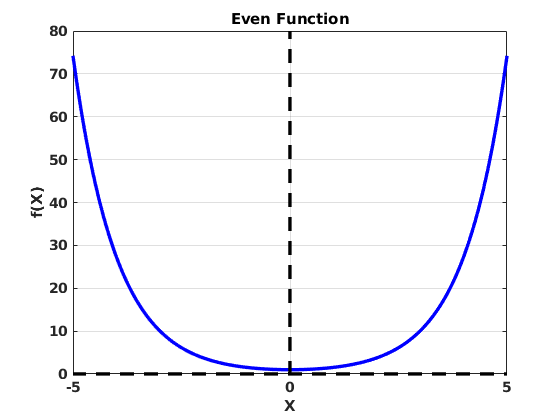
\includegraphics{lec16_even.png}
\caption{An example even function.}
\label{fig:even-fun}
\end{marginfigure}
\begin{marginfigure}
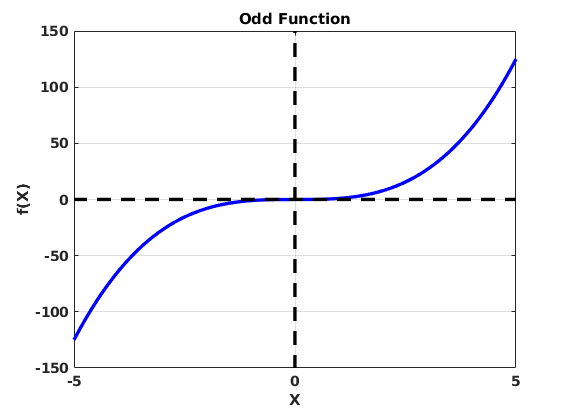
\includegraphics{lec16_odd.png}
\caption{An example odd function.}
\label{fig:odd-fun}
\end{marginfigure}
\begin{definition}[Even Function]
A function is even if, for all real values $x$, $f(-x) = f(x)$.  
\end{definition}
An example of an even function is shown in Figure \ref{fig:even-fun}.
\begin{definition}[Odd Function]
A function is odd if, for all real values $x$, $f(-x) = -f(x)$.
\end{definition}
An example of an odd function is shown in Figure \ref{fig:odd-fun}.

\newthought{Some properties} of even an odd functions include:\sidenote{Students are welcome to prove these assertions.}
\begin{enumerate}
\item An even function times an even function results in an even function.
\item An odd function times an odd function results in an even function.
\item An even function times an odd function results in an odd function.
\item Adding or subtracting two even functions results in an even function.
\item Adding or subtracting two odd functions results in an odd function.
\item $\int_{-p}^{p} f_{\text{even}}(x) \ dx = 2\int_{0}^{p} f_{\text{even}}(x) \ dx$ and $\int_{-p}^{p} f_{\text{odd}}(x) \ dx = 0$.
\end{enumerate}

The ``even-ness'' or ``odd-ness'' of a function is relevant to Fourier series expansions.  If you expand an \emph{even} function in a Fourier series you will find that all of the $b_n$ coefficients are zero.  If you expand an \emph{odd} function in a Fourier series you will find that $a_0$ and $a_n$ terms are all zero.

You can still use the formulas presented in Equation \ref{eq:Fourier-Coeff} when expanding even or odd functions.  Alternatively, you can use the formulas for the Cosine expansion or Sine expansion below for even or odd functions respectively.

\vspace{0.5cm}

\noindent\textbf{Cosine series:}\marginnote{The cosine and sine series expansions are sometimes referred to as ``half-wave'' expansions since the calculations, as shown in the formulas, only involve the portion of the wave in the interval [0,p]---the positive half-wave.}
\begin{align}
\begin{split}
f(x) &= \frac{a_0}{2} + \sum\limits_{n=1}^{\infty}a_n \cos{\frac{n \pi x}{p}} \\
a_0 &= \frac{2}{p}\int_0^p \ f(x) \ dx \\
a_n &= \frac{2}{p} \int_0^p \ f(x) \cos{\frac{n \pi x}{p}} \ dx
\end{split}
\end{align}

\vspace{0.5cm}

\noindent\textbf{Sine series:}
\begin{align}
\begin{split}
f(x) &= \sum\limits_{n=1}^{\infty} b_n \sin{\frac{n \pi x}{p}} \\
b_n &= \frac{2}{p}\int_{0}^{p} \ f(x) \ \sin{\frac{n \pi x}{p}} \ dx
\end{split}
\end{align}


\chapter{Lecture 17 - Generating and Plotting Fourier Series in MATLAB}
\label{ch:lec17}
\section{Objectives}
\begin{itemize}
\item Demonstrate how to carry out Fourier series expansions using MATLAB.
\item Give a qualitative demonstration of convergence behavior of Fourier series.
\item Demonstrate Cosine and Sine series expansions.
\end{itemize}
In this lecture, we will illustrate the process of Fourier series expansions with three examples.

\vspace{0.5cm}

\noindent\textbf{Example \#1:}
Carry out the Fourier series expansion of the function given in Equation \ref{eq:lec17-ex1}, illustrated in Figure \ref{fig:lec17-ex1-fx}:
\begin{equation}
f(x) = 
\begin{cases}
0, & -\pi \le x < 0 \\
\pi - x, & 0 \le x \le \pi
\end{cases}
\label{eq:lec17-ex1}
\end{equation}
\begin{marginfigure}
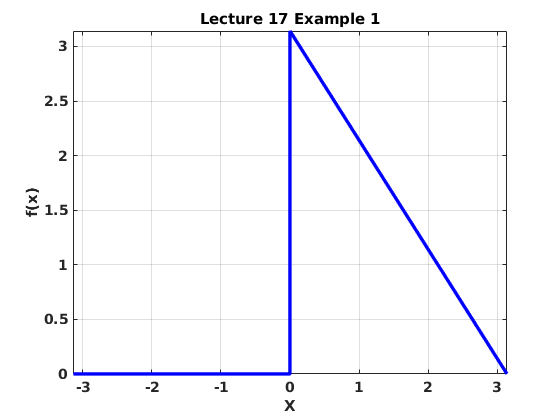
\includegraphics{lec17_ex1_fx.png}
\caption{Example \#1 $f(x)$.}
\label{fig:lec17-ex1-fx}
\end{marginfigure}
We wish to represent this function as:
\begin{equation*}
f(x) = \frac{a_0}{2} + \sum\limits_{n=1}^{\infty} \left[a_n \cos{\frac{n \pi x}{p}} + b_n \sin{\frac{n \pi x}{p}} \right]
\end{equation*}
where, in this case, $p = \pi$.  Even though we are only interested in the function in the interval $[-\pi, \pi]$, since the Fourier series represents the function in terms of a constant and an infinite linear combination of of periodic functions, we should think of the function that we are representing as periodic.\sidenote{This outlook will help us understand the convergence behavior of the Fourier series; especially at the boundaries.}

We have everything we need; it is just a matter of calculating the coefficients from Equation \ref{eq:Fourier-Coeff}.  Rather than carrying out the calculations with pencil and paper we will use MATLAB.  In the listing below we will step through the code necessary to calculate Fourier coefficients through \lstinline{N=5}.

\begin{lstlisting}[name=lec17-ex1,style=myMatlab]
clear
clc
close 'all'

N = 5; % specify number of coefficients

f = @(x) ex1(x); 
p = pi; % specifiy period
\end{lstlisting}
We start, as always, by clearing out the workspace memory and command-prompt output and closing any open figures.  We also need to represent $f(x)$ in MATLAB; we will do this with a local function named \lstinline{ex1(x)}.\sidenote{Since inline functions must appear \emph{after} all of the other code in a MATLAB script file, the code for \lstinline{ex1(x)} will be presented last.}  

The integrals needed to determine the Fourier coefficients will be evaluated numerically with the MATLAB built-in function \lstinline{integral()}.\sidenote{This function has default signature \lstinline{Q = integral(FUN,A,B)} and it approximates the integral of function \lstinline{FUN} over the interval \lstinline{A} to \lstinline{B} using global adaptive quadrature.  The error tolerances for this numeric integration algorithm can be specified by the user; in most cases we will use default values.  There are several standard algorithms for numerically computing integrals---called quadrature---that the interested student can read about in the numerical methods portion of this text.} Let us start with $a_0$ which, as a reminder, is computed by:
\begin{equation*}
a_0 = \frac{1}{p}\int_{-p}^{p} f(x) \ dx
\end{equation*}

\begin{lstlisting}[name=lec17-ex1,style=myMatlab]
a0 = (1/p)*integral(f,-p,p);
FF = @(x) a0/2;
\end{lstlisting}
The first line of the listing numerically evaluates $a_0$; the second line creates an anonymous function and initializes it to the first term in the Fourier expansion.

We will use a loop to construct the remaining terms in the Fourier expansion.\marginnote{Recall:
\begin{align*}
an &= \frac{1}{p}\int_{-p}^p f(x) \cos{\frac{n \pi x}{p}}\ dx \\
bn &= \frac{1}{p}\int_{-p}^p f(x) \sin{\frac{n \pi x}{p}}\ dx
\end{align*}
Note how you can practically read the equation directly from the MATLAB code.
}
\begin{lstlisting}[name=lec17-ex1,style=myMatlab]
for n = 1:N
    an = (1/p)*integral(@(x) f(x).*cos(n*pi*x/p),-p,p);
    bn = (1/p)*integral(@(x) f(x).*sin(n*pi*x/p),-p,p);
    FF = @(x) FF(x) + an*cos(n*pi*x/p) + bn*sin(n*pi*x/p); 
end
\end{lstlisting}
Note in the last line where we append the newly computed terms to the Fourier series expansion \lstinline{FF(x)}.  Now we have a function, $\lstinline{FF(x)}$, that represents the Fourier series expansion with $N=5$ terms.  In the next listing we add the code to plot the function and verify that it makes sense.
\marginnote{

\vspace{2.25cm}

Referring to the annotations:



\noindent \ref{lst:annotation1} Using \lstinline[style=myMatlab]{sprintf()} allows us to combine the variable \lstinline{n} in the title string.  

\vspace{0.25cm}

\noindent \ref{lst:annotation2} Optional name-value pairs such as \lstinline{'Linewidth',3}, \lstinline{'FontSize',16}, and \lstinline{'FontWeight','bold'} help make the plot and labels more readable.



}

\begin{lstlisting}[name=lec17-ex1,style=myMatlab]
Nx = 1000;
X = linspace(-p,p,Nx);

plot(X,f(X),'-b',...
    X,FF(X),'--r',...
    'LineWidth',3)
title_str = sprintf('Example 1, n = %d',n);/*!\annotation{lst:annotation1}!*/
title(title_str,'FontSize',16,...
    'FontWeight','bold');
xlabel('X','FontSize',14,... /*!\annotation{lst:annotation2}!*/
    'FontWeight','bold');
ylabel('f(X)','FontSize',14,...
    'FontWeight','bold');
grid on
legend('f(x)','FF(x)')/*!\annotation{lst:annotation3}!*/
set(gca,'FontSize',12,...
    'FontWeight','bold');/*!\annotation{lst:annotation4}!*/
\end{lstlisting} \marginnote[-2.5cm]{
\vspace{0.25cm}

\noindent \ref{lst:annotation3} Make a habit of using legends for graphs that include multiple data series. Once again, this makes the plot more readable.

\vspace{0.25cm}

\noindent \ref{lst:annotation4} The argument \lstinline[style=myMatlab]{gca} means ``get current axis.''  Calling the \lstinline[style=myMatlab]{set()} function with name-value pairs \lstinline{'FontSize',10} and \lstinline{'FontSize','bold'} sets the font size and weight for the axis markings.

\vspace{0.25cm}

\noindent In general it is important that your plots look good.

}



 \setcounter{lstannotation}{0}
The resulting Fourier series expansion is shown in Figure \ref{fig:lec17-ex1-n5}. If we want to increase the number of Fourier series terms in the expansion, we need only change \lstinline{N}.  Figure \ref{fig:lec17-ex1-n15} shows the series expansion with \lstinline{N=15} terms.
\begin{marginfigure}
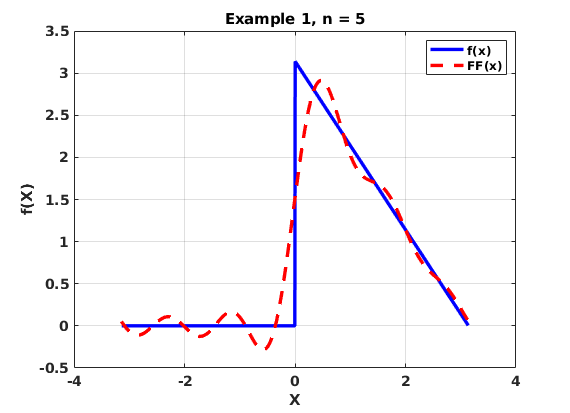
\includegraphics{lec17_ex1_n5.png}
\caption{Fourier series expansion with \lstinline{N=5}.}
\label{fig:lec17-ex1-n5}
\end{marginfigure}

\begin{marginfigure}
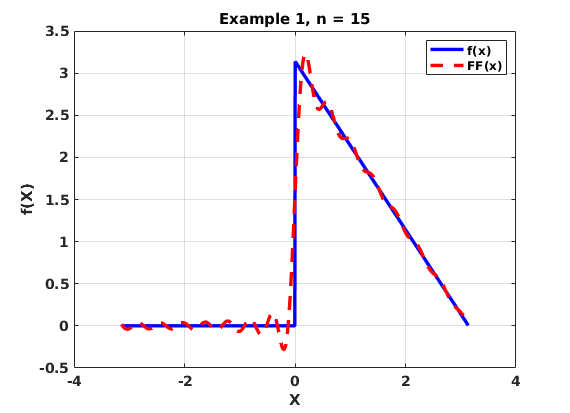
\includegraphics{lec17_ex1_n15.png}
\caption{Fourier series expansion with \lstinline{N=15}.}
\label{fig:lec17-ex1-n15}
\end{marginfigure} 
Some things to note about the resulting Fourier series representation of \lstinline{f(x)}:
\begin{enumerate}
\item As \lstinline{n} increases, \lstinline{FF(x)} generally ``looks more like'' \lstinline{f(x)}.  
\item At the discontinuity in \lstinline{f(x)}, the Fourier series representation appears to be converging on the midpoint between $f(x^-)$ and $f(x^+)$ as the theory says it should.
\item The Fourier series representation near the point of discontinuity has ``wiggliness'' that doesn't go away as \lstinline{n} increases.
\item In particular, note the undershoot and overshoot of $f(x)$ to the left and right respectively of $f(0)$.  This is called ``Gibbs phenomena'' and it does not go away as \lstinline{n} increases but it moves closer to the point of discontinuity.  
\end{enumerate}
As Figure \ref{fig:lec17-ex1-n150} shows, as \lstinline{N} is increased, we can make \lstinline{FF(x)} arbitrarily close to \lstinline{f(x)} with the exception of the perturbations at the point of discontinuity.
\begin{marginfigure}
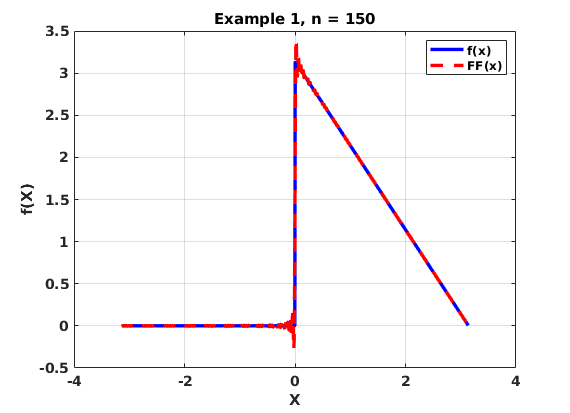
\includegraphics{lec17_ex1_n150.png}
\caption{Fourier series expansion with \lstinline{N=150}.}
\label{fig:lec17-ex1-n150}
\end{marginfigure}

\newthought{An important matter} that we have not yet dealt with is how to represent piece-wise continuous functions like $f(x)$ in MATLAB.\sidenote{For whatever reason, piece-wise continuous functions are intensively used in \emph{textbooks} on partial differential equations---I am not so sure that they are as important in real-life applications.}  As stated previously, we will use a \emph{local function} to do this.  The code is shown in the listing below.

\begin{lstlisting}[name=lec17-ex1,style=myMatlab]
%% Local functions 
function y = ex1(x) 
[m,n] = size(x); /*!\annotation{lst:annotation1-1}!*/
y = nan(m,n); /*!\annotation{lst:annotation1-2}!*/
for i = 1:length(x) /*!\annotation{lst:annotation1-3}!*/
    if (x(i) >= -pi) && (x(i) < 0) 
        y(i) = 0;
    elseif (x(i) >= 0) && (x(i) <= pi) /*!\annotation{lst:annotation1-4}!*/
        y(i) = pi - x(i);
    end
end
end
\end{lstlisting} \setcounter{lstannotation}{0}
Some notes on the annotations for this listing:

\vspace{0.25cm}

\noindent \ref{lst:annotation1-1}  We use the MATLAB built-in function \lstinline[style=myMatlab]{size()} to get the dimensions of the input vector.  The return values \lstinline{[m,n]} give the number of rows and columns of \lstinline{x} respectively. For this function we are implicitly expecting \lstinline{x} to be a vector, but it can be either a row-vector or a column vector.

\vspace{0.25cm}

\noindent \ref{lst:annotation1-2} We construct the output vector \lstinline{y} using the \lstinline{nan()} function.  This line makes the vector \lstinline{y} the same size and shape as the input vector \lstinline{x}.  


\vspace{0.25cm}

\noindent \ref{lst:annotation1-3} We use the built-in function \lstinline[style=myMatlab]{length()} to get the number of elements of \lstinline{x}.  This is a bit of a hack since, if \lstinline{x} were \textbf{\emph{not}} a vector, \lstinline{ex1(x)} would no longer work properly.\sidenote[][-5.0cm]{It would be a good idea to verify that the input \lstinline{x} is actually a vector.  MATLAB, like most other languages, includes features to enforce assumptions like this. The code: \lstinline[style=myMatlab]{assert(min(size(x))==1,'x must be a vector')} would raise an error in MATLAB if the minimum dimension of \lstinline{x} is anything other than 1.  That would be one way to ensure \lstinline{x} is a vector.}

\vspace{0.25cm}

\noindent \ref{lst:annotation1-4} The symbol \lstinline{&&} is ``element-wise and.''  Pay attention to use of \lstinline{>=} and \lstinline{<=} operators to get the details of the intended function correct.

\vspace{0.5cm}

\noindent\textbf{Example \#2:}  Carry out the Fourier series expansion of the function given in Equation \ref{eq:lec17-ex2}, illustrated in Figure \ref{fig:lec17-ex2-fx}.
\begin{equation}
f(x) = 
\begin{cases}
-1, & -\pi \le x < 0 \\
1, & 0 \le x \le \pi
\end{cases}
\label{eq:lec17-ex2}
\end{equation}
\begin{marginfigure}[-6.0cm]
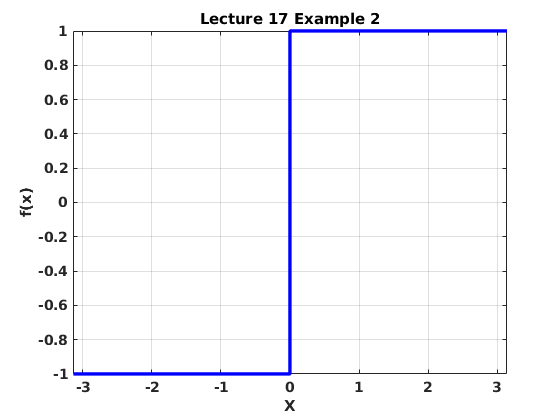
\includegraphics{lec17_ex2_fx.png}
\caption{Example \#2 $f(x)$.}
\label{fig:lec17-ex2-fx}
\end{marginfigure}
Fourier series expansions of this function are shown in Figures \ref{fig:lec17-ex2-n5} through \ref{fig:lec17-ex2-n150}.
\begin{marginfigure}[-1.0cm]
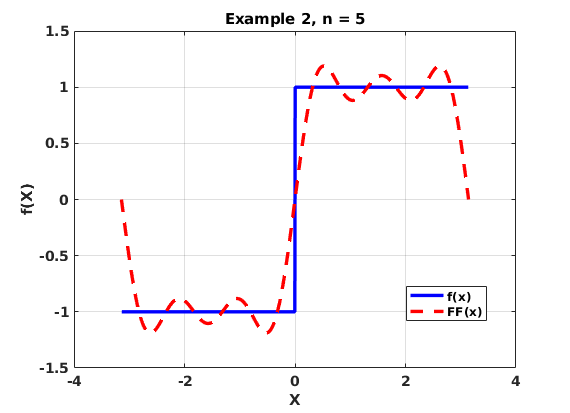
\includegraphics{lec17_ex2_n5.png}
\caption{Fourier series expansion with \lstinline{N=5}.}
\label{fig:lec17-ex2-n5}
\end{marginfigure}

\begin{marginfigure}
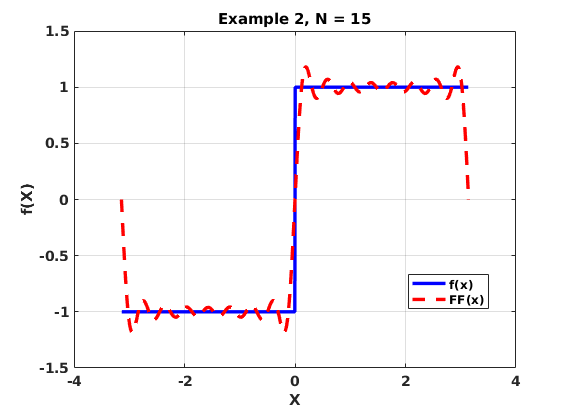
\includegraphics{lec17_ex2_n15.png}
\caption{Fourier series expansion with \lstinline{N=15}.}
\label{fig:lec17-ex2-n15}
\end{marginfigure}

\begin{marginfigure}
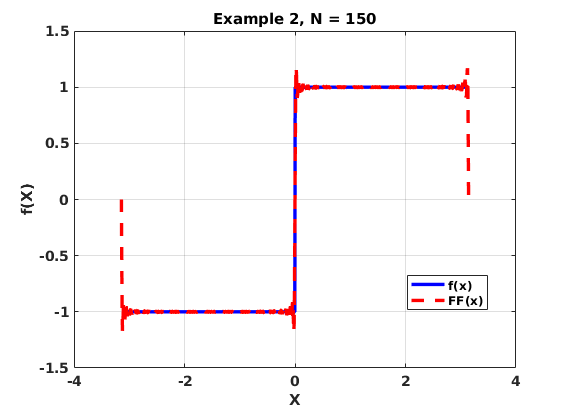
\includegraphics{lec17_ex2_n150.png}
\caption{Fourier series expansion with \lstinline{N=150}.}
\label{fig:lec17-ex2-n150}
\end{marginfigure}
Some notes:
\begin{enumerate}
\item As with the first example, the function has the Gibbs phenomena near the discontinuity at $x=0$.  
\item Also, as with the first example, the Gibbs phenomena does not go away as $N$ increases, but it gets more ``peaked'' and closer to the origin.
\item Unlike the first example, we get the Gibbs phenomena and wiggliness at the ends also.  This is because the Fourier series representation is periodic; the periodic extension of this function has discontinuities at the endpoints since $f(-\pi) \ne f(\pi)$.  
\item You should also note that this function is \emph{even}.  That means we expect $a_0$ and all values of $a_n$ to be equal to zero. If we modify the for-loop to output values for the $a_n$ coefficients we get all zeros.

\begin{lstlisting}[style=myMatlab]
for n = 1:N
    an = (1/p)*integral(@(x) f(x).*cos(n*pi*x/p),-p,p);
    fprintf('a_%d = %g \n',n,an);
    bn = (1/p)*integral(@(x) f(x).*sin(n*pi*x/p),-p,p);
    FF = @(x) FF(x) + an*cos(n*pi*x/p) + bn*sin(n*pi*x/p); 
end
\end{lstlisting}
\end{enumerate}

%\begin{marginfigure}
%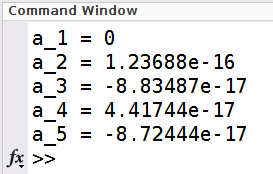
\includegraphics{lec17_ex2_an.png}
%\end{marginfigure}

\vspace{5.0cm}

\noindent\textbf{Example \#3:} Construct the Fourier series expansion of the function given in Equation \ref{eq:lec17-ex3-fx}.

\begin{equation}
f(x) = x^2, \ \ x \in[0,2]
\label{eq:lec17-ex3-fx}
\end{equation}

This function is not periodic and, unlike the previous examples, does not even span a symmetric interval about the origin.  In this case we will still use the same Fourier series formulas but we will construct a ``reflection'' about the origin.  This reflection can be \emph{even-}, \emph{odd-}, or it can be an \emph{identity-reflection} with respect to the y-axis; these correspond to the Cosine expansion, Sine expansion and the full Fourier series expansions.  These different expansion options are shown in Figure \ref{fig:lec17-ex3}.

\begin{figure}
\subfloat[]{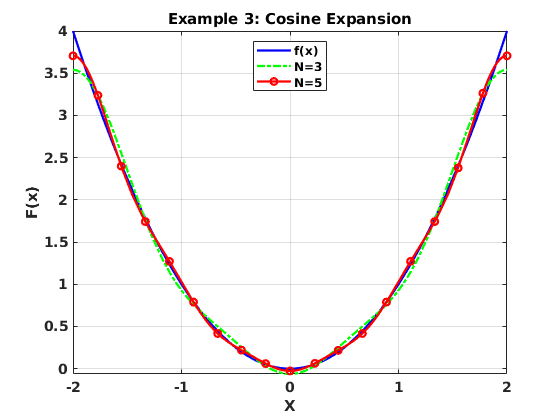
\includegraphics[width=2in]{lec17_ex3_cos.png}}
\subfloat[]{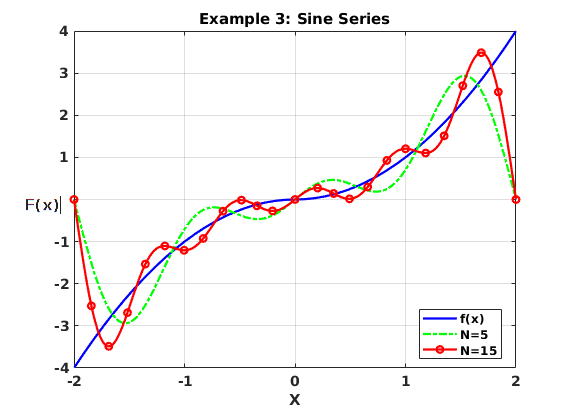
\includegraphics[width=2in]{lec17_ex3_sin.png}} \\
\begin{center}
\subfloat[]{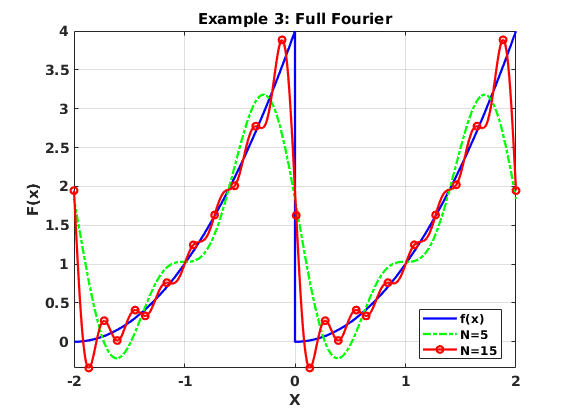
\includegraphics[width=2in]{lec17_ex3_full.png}}
\end{center}
\label{fig:lec17-ex3}
\caption{Even-, odd- and identity-reflection for $f(x)=x^2$.}
\end{figure}

Note that the convergence behavior for the Fourier expansion is different for each case.\marginnote{As you can see, in cases where you can choose which expansion you use, some choices are good and some are bad.  As we will see in coming chapters, we often do not have a choice in which set of orthogonal functions we will use to do our expansion so, sadly, we cannot pick one that we think will be best.  What we \emph{can} do is analyze the expansion that we \emph{do} get and understand the convergence behavior by examining the continuity of the functions and derivatives of functions that we are representing.}
\begin{itemize}
\item For the even-reflection Cosine expansion convergence is very rapid.  Both $f(x)$ and $f^{\prime}(x)$ are continuous throughout the interval $x\in (-2,2)$.  The function itself is continuous at the end-points but notice that the derivative is not.  If you were to draw an additional period on the left and right-hand side of the cosine expansion, $f^{\prime}(x)$ would have a discontinuity; that explains the (relatively) poor convergence of the series at the end-points.
\item For the odd-reflection Sine expansion the function and derivative is continuous throughout the domain.  The derivative of the function is continuous at the periodic end-points but $f(x)$ itself is not.  This explains why the Sine series expansion converges to zero at both end-points.  
\item The identity-reflection full Fourier series has discontinuities in $f(x)$ and $f^{\prime}(x)$ at both endpoints and at $x=0$.  The convergence behavior is correspondingly bad.
\end{itemize}

\chapter{Assignment \#6}
\label{ch:ass6}
\begin{fullwidth}

Show that the given functions are orthogonal on the given interval.
\begin{enumerate}
\item $f_1(x) = e^{x}, \ f_2(x)=xe^{-x}-e^{-x}, \ \ x\in[0,2]$

\vspace{1.0cm}

\item $f_1(x) = x, \ f_2(x)=\cos{2x}, \ \ x\in\left[-\sfrac{\pi}{2},\sfrac{\pi}{2}\right]$
\end{enumerate}

\vspace{1.50cm}

\noindent Show that the given set of functions is orthogonal on the indicated interval.  Find the norm of each function in the set.
\begin{enumerate}[resume]
\item $\left\{\sin{x},\sin{3x},\sin{5x},\dots \right\}, \ \ x\in\left[0,\sfrac{\pi}{2}\right]$

\end{enumerate}

\vspace{1.5cm}

\noindent Use MATLAB to verify by numeric integration that the functions are orthogonal with respect to the indicated weight function on the given interval.

\begin{enumerate}[resume]
\item $H_0(x) = 1, \ H_1(x) = 2x, \ H_2(x)=4x^2-2; \ \ w(x)=e^{-x^2}, \ \ x\in(-\infty,\infty)$

\noindent\textbf{Note:} use the built-in function \lstinline{integral()} to do the numeric integration.  In MATLAB, $-\infty$ and $\infty$ are represented by \lstinline{-inf} and \lstinline{inf} respectively.
\end{enumerate}


\vspace{1.5cm}

\noindent Use MATLAB to construct the Fourier series expansion of the given function $f(x)$ on the given interval.  For each problem create a plot that shows: a) $f(x)$ along with b) the truncated Fourier series of $f(x)$ with \lstinline{N=5} and c) \lstinline{N=15} terms.  Also give the number to which the Fourier series expansion converges at any point(s) of discontinuity in $f(x)$. 

\begin{enumerate}[resume]
\item $f(x) = 
\begin{cases}
0, & -\pi < x < 0 \\
1, & 0 \le x < \pi
\end{cases}$


\vspace{1.0cm}

\item $f(x) = 
\begin{cases}
0, & -\pi < x < 0 \\
x^2, & 0 \le x < \pi
\end{cases}$

\vspace{1.0cm}

\item $f(x) = 
\begin{cases}
0, & -2 < x < 0 \\
-2, & -1 \le x < 0 \\
1, & 0 \le x < 1 \\
0, & 1 \le x < 2
\end{cases}$

\end{enumerate}

\vspace{1.5cm}

\noindent Determine whether the given function is even, odd, or neither.
\begin{enumerate}[resume]
\item $f(x) = x^2+x$

\vspace{1.0cm}

\item $f(x) =
\begin{cases}
x^2, & -1 < x < 0 \\
-x^2, & 0 \le x < 1
\end{cases}$
\end{enumerate}

\vspace{1.5cm}

\noindent Use MATLAB to expand the given function in an appropriate cosine or sine series.  For each function create a plot showing: a) $f(x)$ along with b) the truncated Fourier series of $f(x)$ with \lstinline{N=5} and; c) \lstinline{N=15} terms.

\begin{enumerate}[resume]
\item $f(x) = \left| x \right|, \ \ -\pi < x \pi$

\vspace{1.0cm}

\item $f(x) = 
\begin{cases}
x-1, & -\pi < x < 0 \\
x+1, & 0 \le x < \pi
\end{cases}$

\vspace{1.0cm}

\item $f(x) = 
\begin{cases}
1, & -2 < x < -1 \\
-x, & -1 \le x < 0 \\
x, & 0 \le x < 1 \\
1, & 1 \le x < 2
\end{cases}$

\vspace{1.0cm}

\item $f(x) = 
\begin{cases}
x, & 0 < x < \sfrac{\pi}{2} \\
\pi - x, & \sfrac{\pi}{2} \le x < \pi
\end{cases}$
\end{enumerate}

\end{fullwidth}

\chapter{Lecture 18 - Sturm-Liouville Problems}
\label{ch:lec18}
\section{Objectives}
\begin{itemize}
\item Define regular/singular Sturm-Liouville eigenvalue problems and give properties of their solutions.
\item Do an example problem for finding eigenvalues and eigenfunctions.
\item Do an example problem for transforming a linear, second-order, homogeneous boundary value problem into self-adjoint form.
\end{itemize}

\section{Regular Sturm-Liouville Eigenvalue Problem} \index{Sturm-Liouville Eigenvalue Problem}
We have solved several differential equations in this class.  All of the boundary value problems that we have solved so far are special cases of a more general framework called Sturm-Liouville eigenvalue problems. That is what we wish to discuss in this lecture.

For the regular Sturm-Liouville Eigenvalue problem we hope to solve:\marginnote{\textbf{Note:} for Equation \ref{eq:sturm-liouville-evp}, $r(x)$, $r^{\prime}(x)$, $q(x)$, and $p(x)$ must be real-valued and continuous on the interval $x \in (a,b)$.  Also $p(x)>0$ and $r(x)>0$ for all $x\in(a,b)$.  These are important conditions that should be verified each time you encounter a new problem.  The constant $\lambda$ is referred to as an \emph{eigenvalue}.}
\begin{equation}
\frac{d}{dx}\left[r(x)u^{\prime}\right] + \left(q(x) + \lambda p(x)\right)u = 0,  \ \ x\in(a,b)
\label{eq:sturm-liouville-evp}
\end{equation}
subject to the boundary conditions:
\begin{align*}
A_1u(a) + B_1u^{\prime}(a) &= 0, \text{ where }A_1,\text{ and }B_1\text{ are not both zero.} \\
A_2u(b) + B_2u^{\prime}(b) &= 0, \text{ where }A_2,\text{ and }B_2\text{ are not both zero.}
\end{align*}
Note that these boundary conditions are referred to as \emph{homogeneous}.  The same rule that we use to decide if a differential equation is homogeneous apply in the same way to the boundary conditions.\marginnote[-1.0cm]{For ODEs that we solved in earlier lectures, we routinely dealt with problems having non-homogeneous boundary conditions.  As we go forward to solve linear partial differential equations using separation of variables, it will be \emph{essential} that the boundary conditions are homogeneous.  So you should be sure that you know how to check/verify that condition.}  For a boundary value problem to be homogeneous, \emph{both} the differential equation \emph{and} boundary conditions must be homogeneous.

\vspace{5.0cm}

\noindent\underline{Properties of the Regular Sturm-Liouville problem:}
\begin{enumerate}
\item There exist an infinite number of real eigenvalues that can be arranged in increasing order. (e.g. $\lambda_1 < \lambda_2 < \lambda_3 < \cdots < \lambda_n < \cdots$)
\item For each eigenvalue, $\lambda_n$, there is exactly one eigenfunction, $u_n(x)$, that is a solution to the problem.

\item Eigenfunctions corresponding to different eigenvalues are linearly independent.

\item The set of eigenfunctions is orthogonal with respect to $p(x)$ on the interval $[a,b]$.  In other words: $\int_{a}^{b}u_n(x) u_m(x) p(x) \ dx = 0$ if $n \ne m$.

\item The set of eigenfunctions is complete on the interval $[a,b]$.  In other words, for any (reasonable) $f(x)$, we can represent $f(x)$ as a linear combination of those eigenfunctions: $f(x) = \sum_{n=0}^{\infty} c_n u_n(x)$.\sidenote{Another way of saying this is that no function, $f(x)$, can be orthogonal to \emph{all} of the eigenfunctions, $u_n(x)$, on the interval $[a,b]$.

To obtain values for the coefficients, $c_n$, we need only take the inner product with the corresponding eigenfunction, $u_n$.  i.e. multiply both sides by an orthogonal function and integrate.}
\end{enumerate}


\newthought{If $r(x)$ in} Equation \ref{eq:sturm-liouville-evp} is zero at either boundary, the problem is said to be a singular boundary value problem.  If $r(a) = r(b)$, with suitable boundary conditions, the problem is said to be a periodic boundary value problem.

\vspace{1.0cm}

\noindent\textbf{Example:} Find the eigenvalues and eigenfunctions of the following boundary value problem:\marginnote{Note that this problem is not presented in self-adjoint form.  Have faith that it is, indeed, a Sturm-Liouville eigenvalue problem and could be presented in self-adjoint form.  We will practice making this transformation later in the lecture.}
\begin{align*}
\text{Equation: }& & u^{\prime \prime}+\lambda u = 0,  \ \ x\in[0,1] \\
\text{BCs: }& & u(0) = 0, \ \ u(1) + u^{\prime}(1) = 0
\end{align*}
To fully analyze this problem we will have to consider three cases for $\lambda$: $\lambda < 0$, $\lambda = 0$, and $\lambda > 0$.

\vspace{0.5cm}

\noindent \underline{$\lambda = 0$:}  In this case, the differential equation reduces to:
\begin{equation*}
u^{\prime \prime} = 0
\end{equation*}
with general solution: $u(x) = c_1(x) + c_2$.  If we apply the boundary condition $u(0) = 0$, this implies that $u(0) = c_1(x) + c_2 = c_2 = 0$. So the solution is simplified to $u(x) = c_1(x)$.  The second boundary condition: $u(1) + u^{\prime}(1) = c_1(1) + c_1 = 2c_1 = 0 \Rightarrow c_1 = 0$. The only solution that satisfies the equation and boundary conditions for $\lambda = 0$ is the trivial solution $u(x) = 0$.\sidenote[][-1.5cm]{The trivial solution, $u(x)=0$ will always satisfy a homogeneous boundary value problem and, in general, is of little interest to us.  What we take from this part of the analysis is that we will rule out $\lambda=0$ since there are no \emph{interesting} solutions in that case.}

\vspace{4.5cm}

\noindent\underline{$\lambda < 0$:}  For this case we will assume $\lambda = -\alpha^2$ where $\alpha > 0$.  The differential equation reduces to:
\begin{equation*}
u^{\prime \prime} - \alpha^2u = 0
\end{equation*}
This equation has the general solution of:\marginnote[0.75cm]{Recall that these two solutions are equivalent.  We will generally use the first form on \emph{unbounded} intervals; the second form on \emph{bounded} intervals.}
\begin{align*}
u(x) &= c_1e^{-\alpha x} + c_2e^{\alpha x} \\
\text{ or: } & \\
u(x) &=c_1 \cosh{\alpha x} + c_2 \sinh{\alpha x} 
\end{align*}
Since this problem is posed on a bounded interval, we will choose the second form above.  Applying the first boundary condition gives us: $u(0) = c_1\cosh{0} + c_2\sinh{0} = c_1(1) + c_2(0) = 0 \Rightarrow c_1 = 0$.  Applying the second boundary condition to the current solution gives us: $u(1) + u^{\prime}(1) = c_2\sinh{1} + c_2\cosh{1} = 0$. \begin{marginfigure} 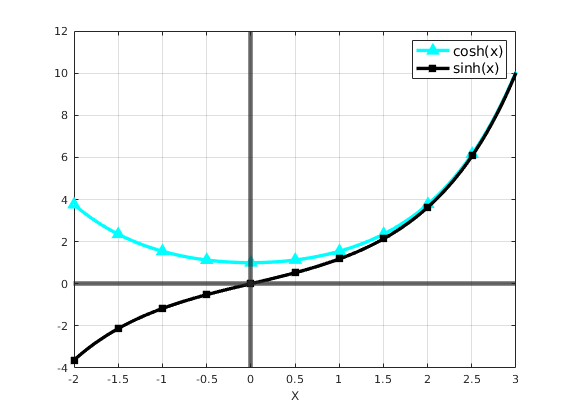
\includegraphics{cosh_and_sinh_plot.png} \end{marginfigure}  
We recall that both $\sinh{x}$ and $\cosh{x}$ are strictly positive on $x\in(0,1)$ so the only way the second boundary condition can be met is for $c_2 = 0$.  Consequently only the trivial solution, $u(x) = 0$, satisfies the governing equation and boundary conditions for the case that $\lambda < 0$.

\vspace{0.5cm}

\noindent\underline{$\lambda > 0$:} For this case we will assume $\lambda = \alpha^2$ where $\alpha > 0$.  The differential equation reduces to:
\begin{equation*}
u^{\prime \prime} + \alpha^2 u = 0
\end{equation*}
This equation has the general solution of $u(x) = c_1 \cos{\alpha x} + c_2 \sin{\alpha x}$.  Applying the first boundary condition gives us: $u(0) = c_1 \cos{0} + c_2 \sin{0} = c_1(1) + c_2(0) = 0 \Rightarrow c_1 = 0$.  Applying the second boundary condition t the current solution gives us: $u(1) + u^{\prime}(1) = c_2 \sin{\alpha} + \alpha c_2 \cos{\alpha} = 0$, or:
\begin{equation}
u(x) = c_2\left[\sin{\alpha} + \alpha \cos{\alpha}\right] = 0
\label{eq:lec18-ex1}
\end{equation}
This equation can be satisfied simply by setting $c_2 = 0$, but we will resist that temptation since that would then imply that there are \emph{no} values of $\lambda$ that admit a non-trivial solution for this problem.  Instead we will look for values of $\alpha$ such that:
\begin{equation}
\sin{\alpha} + \alpha \cos{\alpha} = 0
\label{eq:lec18-ex1-ev-eq}
\end{equation}
\begin{marginfigure}
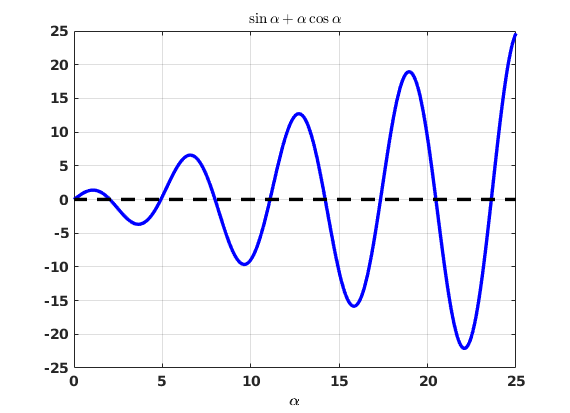
\includegraphics{lec18_evplot.png}
\caption{Plot of $\sin{\alpha} + \alpha \cos{\alpha}$.}
\label{fig:lec18-evplot}
\end{marginfigure}
We can see from Figure \ref{fig:lec18-evplot} that there are values of $\alpha$ that satisfy this condition.\sidenote{We probably should not assume as much by looking at the plot in Figure \ref{fig:lec18-evplot} but it turns out that there are infinitely many zeros.}  We will denote these eigenvalues $\alpha_1^2 = \lambda_1$, $\alpha_2^2 = \lambda_2$, $\dots$, $\alpha_n^2 = \lambda_n$ and the corresponding eigenfunctions are denoted: $u_n(x) = \sin{\alpha_n x}$.

\newthought{We will defer,} for the moment, the problem of finding the roots to Equation \ref{eq:lec18-ex1-ev-eq}. Suffice it to say that there are infinitely many distinct roots yielding the infinitely many eigenvalues to go with the infinitely many eigenfunctions. They can be found with a non-linear equation solver (``root-finder'') for which there are several reliable algorithms.

\section{Transforming Equations to Self-Adjoint Form}
Apart from sharing some theoretical tid-bits regarding Sturm-Liouville eigenvalue problems, the \emph{point} of this lecture is to highlight: a) the eigenfunctions that solve the eigenvalue problem; and b) their property of weighted orthogonality.  Recalling the last two lectures where we used an infinite set of trigonometric functions for functional expansion in a Fourier series, we will want to use \emph{other} functions for such expansions. Those other functions will be the set of eigenfunctions associated with a Sturm-Liouville eigenvalue problem.   

As previously mentioned, the eigenfunction solutions are linearly independent and orthogonal with respect to weight function $p(x)$.  We need to know what that weight function is in order to carry out an orthogonal function expansion like Fourier series.\marginnote{The sines and cosines used in Fourier series fit within this theory.  It turns out that the weight function $p(x)$ in that case is $p(x)=1$.}  

\newthought{Consider the linear,} homogeneous, second-order boundary value problem shown in Equation \ref{eq:lin-homo-bvp}:

\begin{equation}
a(x)u^{\prime \prime} + b(x)u^{\prime} + (c(x) + \lambda d(x))u = 0
\label{eq:lin-homo-bvp}
\end{equation}
where $a(x) \ne 0$ and $a(x)$, $b(x)$, $c(x)$, and $d(x)$ are continuous.  We will convert to the self-adjoint form:$\frac{d}{dx}\left[r(x)u^{\prime}\right]+[q(x)+\lambda p(x)]u =0$ by determining the functions $r(x)$, $q(x)$, and $p(x)$ as follows:
\begin{enumerate}
\item $r(x) = e^{\int \sfrac{b(x)}{a(x)} \ dx}$
\item $q(x) = \frac{c(x)}{a(x)}r(x)$
\item $p(x) = \frac{d(x)}{a(x)}r(x)$
\end{enumerate}

\vspace{5.5cm}

\noindent\textbf{Example:} Express the following equation, which has solutions $P_n(x)$ in self-adjoint form and give the orthogonality relation.\marginnote{This is Legendre's equation that we solved in a previous lecture.  $P_n(x)$ is standard notation for Legendre polynomials of order $n$.}

\begin{equation*}
\underbracket{\left(1-x^2\right)}_{a(x)}u^{\prime \prime} \underbracket{- 2x}_{b(x)}u^{\prime}+\overbracket{n(n+1)}^{\lambda}u = 0, \ \ x\in(-1,1)
\end{equation*}
From the equation, $a(x)$ and $b(x)$ are annotated; $c(x) = 0$ and $d(x) = 1$.  We first compute $r(x)$:\marginnote[0.85cm]{Here we use a $u$-substitution:
\begin{align*}
u &= \left(1-x^2\right) \\
du &= -2x \ dx 
\end{align*}
so $e^{\int \frac{-2x}{\left(1-x^2\right)} \ dx}$ = $e^{\int \frac{1}{u} \ du} $ following this substitution.
}
\begin{align*}
r(x) &= e^{\int \frac{-2x}{\left(1-x^2\right)} \ dx} \\
&= e^{\int \frac{1}{u} \ du }\\
&= e^{\ln{u}} \\
&= u \\
&= 1-x^2
\end{align*}
Now we compute $q(x):$
\begin{align*}
q(x) &= \frac{c(x)}{a(x)}r(x) \\
&= \frac{0}{\left(1-x^2\right)}\left(1-x^2\right) \\
&= 0
\end{align*}
Then $p(x)$:
\begin{align*}
p(x) &= \frac{d(x)}{a(x)} r(x) \\
&= \frac{1}{\left(1-x^2\right)}\left(1-x^2\right) \\
&= 1
\end{align*}
Therefore the boundary value problem in self-adjoint form is:
\begin{equation}
\frac{d}{dx}\left[\left(1-x^2\right)u^{\prime} \right]+\lambda_n u = 0
\end{equation}
where $\lambda_n = n(n+1)$.
As given in the problem statement, the eigenfunctions are $P_n(x)$ and the weight function $p(x) = 1$.  The orthogonality relation is:\marginnote[1.5cm]{\textbf{Note:} You will not be expected to know, by inspection, the value of $\left(P_n,P_n\right)$ but it is provided here for your information.}
\begin{equation*}
\left(P_m,P_n\right) = \int_{-1}^{1} \ P_m(x) P_n(x) (1) \ dx = 
\begin{cases}
0, & m \ne n \\
\frac{2}{2n+1}, & m = n
\end{cases}
\end{equation*}


\chapter{Lecture 19 - Fourier-Bessel Series Expansions}
\label{ch:lec19}
\section{Objectives}
\begin{itemize}
\item Present the parametric Bessel equation as a Sturm-Liouville problem and derive the orthogonality relation.
\item Do an example to show a Fourier-Bessel expansion of a function.
\item Demonstrate use of the MATLAB function \lstinline{besselzero()}.
\end{itemize}

\section{Parametric Bessel Equation}
The parametric Bessel equation is a second-order linear, homogeneous differential equation that also fits within Sturm-Liouville theory.  As a reminder, the equation is:
\begin{equation*}
x^2u^{\prime \prime} + xu^{\prime} + \left(\alpha^2x^2-\nu^2\right)u = 0
\end{equation*}
and the general solution is given by:
\begin{equation*}
u(x) = c_1J_{\nu}(\alpha x) + c_2Y_{\nu}(\alpha x)
\end{equation*}

\noindent The solutions, $J_{\nu}(\alpha x)$ and $Y_{\nu}(\alpha x)$ are, of course, linearly independent but they also are orthogonal with respect to some weight function $p(x)$.  We can use them to construct an orthogonal function expansion in exactly the same way we did with Fourier series.  That is what we will do in this lecture.  To accomplish this we want to put the parametric Bessel equation in self-adjoint form and we will proceed in this effort just as we did in the last lecture.

\vspace{0.5cm}

\noindent Let us first put the parametric Bessel equation in standard form:\marginnote{It may not be clear immediately that $\lambda$ corresponds to values of $\alpha$ but that is the correct inference; when we do the orthogonal function expansion with Bessel functions it will be more clear why that is the case.}
\begin{align*}
a(x)u^{\prime \prime} + b(x)u^{\prime} + \left[c(x)+\lambda d(x) \right] u &= 0 \\
x^2u^{\prime \prime} + xu^{\prime} + \left[-\nu^2 + \alpha^2 x^2\right]u &=0
\end{align*}
so, $a(x) = x^2$, $b(x)=x$, $c(x) = -\nu^2$, and $d(x)=x^2$.

\vspace{0.25cm}

\noindent Next we will compute $r(x)$:
\begin{align*}
r(x) &= e^{\int \frac{b(x)}{a(x)} \ dx} \\
&= e^{\int \frac{x}{x^2} \ dx} \\
&= e^{\int \frac{1}{x} \ dx} \\
&= e^{\ln{x}} \\
&= x
\end{align*}

\vspace{0.25cm}

\noindent Now we compute $q(x)$:
\begin{align*}
q(x) &= \frac{c(x)}{a(x)}r(x) \\
&= \frac{-\nu^2}{x^2}x \\
&= -\frac{\nu^2}{x}
\end{align*}

\vspace{0.25cm}

\noindent Then $p(x)$:
\begin{align*}
p(x) &= \frac{d(x)}{a(x)}r(x) \\
&=\frac{x^2}{x^2}x \\
&= x
\end{align*}
So the self-adjoint form of the parametric Bessel equation is:\marginnote{Admittedly, the real reason why we want to do this is to obtain the weight function $p(x)$ which, in this case is $p(x)=x$.}
\begin{equation*}
\frac{d}{dx}\left[x u^{\prime} \right] + \left(-\frac{\nu^2}{x} + \alpha^2 x \right)u = 0
\end{equation*}
The corresponding orthogonality relation is shown in Equation \ref{eq:fb-ortho}:\marginnote{Like other Sturm-Liouville problems we will find that there are infinitely many distinct eigenvalues, $\lambda_n$, which for this equation we will refer to as $\alpha_n$.  Note the weight function $x$ now appears in the inner product.}
\begin{equation}
\int_{a}^{b}J_{\nu}(\alpha_n x) J_{\nu}(\alpha_m x) x \ dx = 0, \ \ n \ne m
\label{eq:fb-ortho}
\end{equation}
where $a$ and $b$ are the bounds of the interval on which orthogonality is expressed.

\vspace{0.5cm}

\noindent\textbf{Example:} Expand $f(x)=x, \ 0<x<3$, in a Fourier-Bessel series, using Bessel functions of order $\nu=1$ that satisfy the boundary condition $J_{1}(3\alpha)=0.$\marginnote[-1.25cm]{Remember that it is the \emph{boundary conditions} that allow us to determine the eigenvalues.}

\vspace{0.25cm}
\begin{marginfigure}
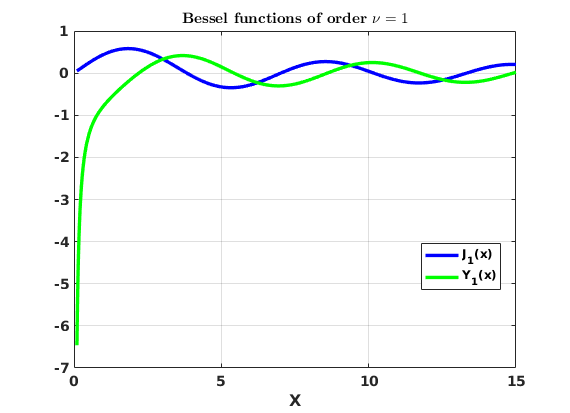
\includegraphics{lec19_bessel1_plot.png}
\label{fig:lec19-bessel}
\caption{Bessel functions of order 1.}
\end{marginfigure}
\noindent So what we want is:
\begin{equation*}
f(x) = x = \sum\limits_{n=1}^{\infty}c_n J_{1}\left(\alpha_n x\right)
\end{equation*}
Note that we omit Bessel functions of the second kind, $Y_n(x)$, because as is shown in the figure, they diverge to negative infinity as $x$ goes to zero.  This \emph{implicit boundary condition}, where one solution of the differential equation diverges at the problem boundary, often needs to be considered when solving boundary value problems.

The other boundary condition applies at $x=3$: $J_{1}(3\alpha_n) = 0$ or, put differently, we select the values of $\alpha_n$ such that $3\alpha_n$ is a root of $J_{1}(x)$.  While our plot of $J_1(x)$ does not extend out to infinity, it turns out that $J_1(x)$ has infinitely many roots and we need to find them.

\subsection{Interlude on Open-Source Software}
At some point in time in your life as an engineer it is inevitable that a problem will arise that you are not prepared to tackle yourself. The tools you have been given to do your job do not fully answer to the task at hand.  This is one such occasion.  We need to find the roots of $J_1(x)$.  \emph{You know} those values exist but you do not know what they are and it turns out that MATLAB does not (at this time) have any built-in functions to give you the roots of such functions either.\sidenote[][-2.0cm]{MATLAB \emph{does} have built-in functions to represent several types of Bessel functions; $J_{\nu}(x)$ and $Y_{\nu}(x)$ are represented, respectively, by \lstinline[style=myMatlab]{besselj(nu,x)} and \lstinline[style=myMatlab]{bessely(nu,x)}. We will learn about more Bessel functions in future lectures.}

\vspace{0.15cm}

\noindent Some options available to you include:
\begin{enumerate}
\item Go to the library and check out a book that tabulates some roots of $J_{1}(x)$---possibly also including scads of additional Bessel function lore\cite{bowman2012introduction}---and enter the desired roots by hand into your MATLAB code.
\item Implement an algorithm to find the roots of $J_1(x)$, possibly using a root-finding tool in MATLAB such as \lstinline[style=myMatlab]{fzero()} or \lstinline[style=myMatlab]{fsolve()}.
\item Find a third-party function or library that has already been written that solves the problem.
\end{enumerate}
In this case we will take the last option since, it turns out, someone \emph{has} already solved this problem for us\marginnote[-0.5cm]{The Fourier-Bessel expansion that we are learning about in this lecture is a standard element in the analytical methods repertoire; \emph{of course} someone else has already figured out how to find the roots of Bessel functions.} and it is a safe bet that they did a better job than what we would be prepared to do.  The MATLAB file exchange is an online repository where people can freely share code that they find useful and other users can look there in search of helpful code when needed.\sidenote{Note that a (free) MathWorks account is required to use the MATLAB file exchange.} 

\newthought{Regarding Open-Source} software:
we have a lot of experience with proprietary software. From operating systems like Microsoft Windows or Apple's IOs to office productivity tools like Microsoft Word or Excel, to valuable and important engineering tools like MATLAB or COMSOL.  We also have experience with free software, such as many applications that you download onto your smartphones.  I want to write a few words in hopes of dispelling any negative connotations that you may have developed in relation to open-source software in comparison to proprietary software.
\begin{itemize}
\item Scientists and engineers of all types---not just computer scientists---write and share software in an open-source framework.  Online repositories like GitHub and GitLab are meant expressly for developing code in an open and collaborative way and then sharing the results freely.
\item ``open-source'' ensures the source code is available.  Sometimes the code is also free but that is not the essential part.\sidenote{Think: ``free speech,'' not ``free beer.''}

\item Open-source software is a \emph{hugely} important contribution to science.  Free and open-source tools like:
\begin{itemize}
\item The \LaTeX\ typesetting tools and almost all of the other software installed on the computer used to prepare this manuscript, including the Linux operating system, are free and open-source software.\sidenote{MATLAB is a notable exception to this list.  There is a free and open-source alternative called Octave. \url{https://octave.org/} }
\item Programming languages that have been a part of the scientific computing landscape for generations.  Examples include Python, C++, Java and FORTRAN among others.
\item OpenMC\cite{ROMANO201590} - a powerful particle transport simulation tool similar to MCNP.
\item MOOSE - \underline{M}ulti-physics \underline{O}bject-\underline{O}riented \underline{S}imulation \underline{E}nvironment\cite{lindsay2022moose} combines the open-source finite element library libMesh\cite{kirk2006libmesh} and the \underline{P}ortable, \underline{E}xtensible \underline{T}oolkit for \underline{S}cientific \underline{C}omputation (PETSc)\cite{petsc-user-ref} along with a host of other free, open-source libraries to create an enormously powerful and flexible tool-set that is used to create the majority of all new multi-physics nuclear analysis codes in the United States.\sidenote{For a list of current applications tracked by the MOOSE development team see: \url{https://mooseframework.inl.gov/application_usage/tracked_apps.html}.  Not all of these codes are open-source, but they have all been created with open-source tools.}
\end{itemize} 
\item As the previous item should help illustrate, open-source software can be of very high quality.  The developers of MOOSE-based applications at the Department of Energy labs are highly trained scientists following nuclear quality assurance standards to ensure that the resulting software tools work correctly and do what they are supposed to do. 

 

\end{itemize}
If you have any interest in scientific computing, now is a good time to develop an interest in open-source software.

\subsection{Back to the Example}
We want to expand $f(x)=x$ for $0<x<3$ in a Fourier-Bessel series expansion using Bessel functions of the first kind of order 1 that satisfy the boundary condition: $J_{1}(3\alpha_n)=0$.  We will use MATLAB along with the function \lstinline[style=myMatlab]{besselzero()} that we obtained from the MATLAB file exchange to carry out this task. In particular we will compute the truncated expansion with $N=15$ terms:
\begin{equation*}
f(x) = x = \sum\limits_{n=1}^{15}c_n J_1\left(\alpha_n x\right)
\end{equation*}

\begin{enumerate}
\item Use \lstinline[style=myMatlab]{besselzero()} to get $\alpha_1,\alpha_2,\dots,\alpha_N$ for our expansion.

\begin{lstlisting}[name=lec19_ex, style=myMatlab]
clear
clc
close 'all'

N = 15; % number of eigenvalues
a = 0; b = 3; % bounds of the domain
nu = 1; kind = 1;
k = besselzero(nu,N,kind); % get roots  /*!\annotation{lst:annotation19-1}!*/
alpha = k/b;  /*!\annotation{lst:annotation19-2}!*/
\end{lstlisting}
\marginnote[-1.5cm]{\ref{lst:annotation19-1} \lstinline[style=myMatlab]{besselzero()} takes up to three arguments; the first,$\nu$, is the order of the Bessel function; the second is the number of roots requested; the third is to indicate the \emph{kind}---first or second---of Bessel function for which you want the roots.

\vspace{0.25cm}
\ref{lst:annotation19-2} since $J_1\left(\alpha_n 3\right) = k_n$ where $k_n$ is the n\textsuperscript{th} root of $J_1$, $\alpha_n$ must be equal to $\sfrac{k_n}{3}$.

}

Now we have the first \lstinline{N=15} values of $\alpha_n$.

\item Compute the coefficients of the expansion $c_n$.  As with the Fourier series, we do this by multiplying both sides of our equation by an orthogonal function \emph{and the weight function } $p(x)=x$ and integrating. For example, to get $c_1$, we do the following:
\begin{align*}
f(x) = x &= c_1 J_1\left(\alpha_1 x\right) + c_2 J_1 \left(\alpha_2 x\right) + \cdots \\
\int_0^3 x J_1\left(\alpha_1 x\right) x \ dx &= c_1 \int_0^3 J_1\left(\alpha_1 x\right)^2 x \ dx + c_2 \underbracket{\int_0^3 J_1\left(\alpha_2 x \right) J_1 \left( \alpha_1 x \right) x \ dx}_{=0 \ \text{by orthogonality}} + \cdots \\
\Rightarrow c_1 &= \frac{\int_0^3 x J_1\left(\alpha_1 x\right) x \ dx}{\int_0^3 J_1\left(\alpha_1 x\right)^2 x \ dx}
\end{align*}
where we recall that the weight function for the orthogonality relation for the Bessel equation is $p(x)=x$.  For the calculation of $c_1$ all of the remaining terms are zero due to the weighted orthogonality of the eigenfunctions $J_1\left(\alpha_n x \right)$.  We repeat the process for all values of $c_n$ and, in MATLAB, we implement this process in the form of a loop.
\marginnote[3.0cm]{
\ref{lst:annotation19-3} these three lines are actually one long line of MATLAB that calculates the coefficients:
\begin{equation*}
c_n = \frac{\int_0^3 x J_1\left(\alpha_1 x\right) x \ dx}{\int_0^3 J_1\left(\alpha_1 x\right)^2 x \ dx}
\end{equation*}
}
\begin{lstlisting}[name=lec19_ex,style=myMatlab]
f = @(x) x; 
cn = nan(N,1); % store the coefficients (optional)

FB = @(x) 0; % initialize the Fourier-Bessel expansion
for n = 1:N
    % compute the i-th coefficient
    cn(n) =...
     integral(@(x) f(x).*besselj(nu,alpha(n)*x).*x,a,b)./... /*!\annotation{lst:annotation19-3}!*/
     integral(@(x) x.*besselj(nu,alpha(n)*x).^2,a,b);
    % update the Fourier-Bessel expansion
    FB = @(x) FB(x) + cn(n)*besselj(nu,alpha(n)*x); 
end
end
\end{lstlisting}
\end{enumerate}
We are now ready to plot the resulting Fourier expansion.\marginnote[0.75cm]{
\ref{lst:annotation19-4} Create a vector to represent the $x$-axis.}

\begin{lstlisting}[name=lec19_ex,style=myMatlab]
Nx = 1000;
X = linspace(a,b,Nx); /*!\annotation{lst:annotation19-4}!*/

figure(1)
plot(X,FB(X),'-b','LineWidth',3);
xlabel('X','fontsize',14,'fontweight','bold');
ylabel('f(X)','fontsize',14,'fontweight','bold');
titlestr = sprintf('Fourier-Bessel expansion, N = %d',N);
title(titlestr,'fontsize',16,'fontweight','bold');
grid on
set(gca,'fontsize',12,'fontweight','bold');

\end{lstlisting}
\begin{marginfigure}
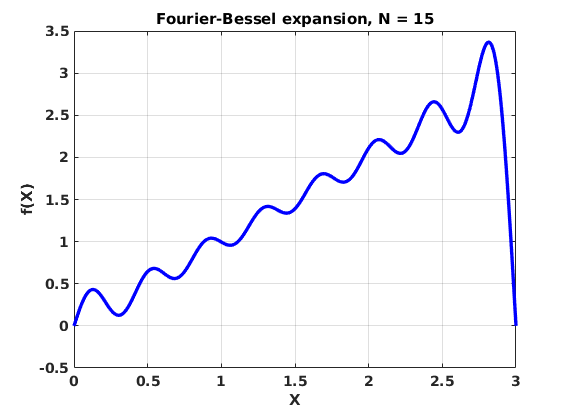
\includegraphics{lec19_ex1_N15.png}
\caption{Fourier-Bessel expansion of $f(x)=x$.}
\label{fig:lec19-ex1-n15}
\end{marginfigure}
The Fourier-Bessel expansion of $f(x)=x$ with $N=15$ is shown in Figure \ref{fig:lec19-ex1-n15}.  Note that the expansion for $N=15$ looks pretty rough. There are many wiggles through the domain and the expansion drops suddenly to zero as the function approaches $x=3$.  The reason for this is that \emph{it had to.}  We are building the expansion with orthogonal functions that are all equal to zero at $x=3$.  Of course $f(x)=x$ is equal to 3 at $x=3$ so something had to give.  

\begin{marginfigure}
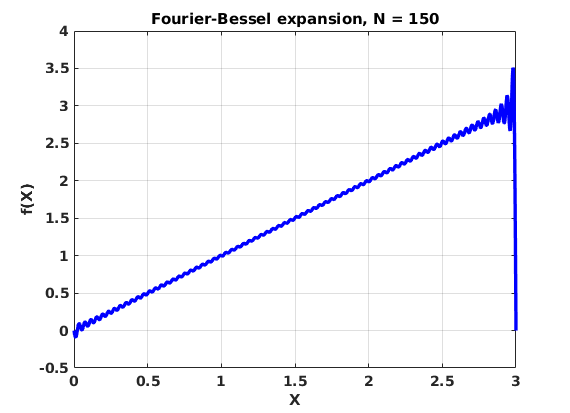
\includegraphics{lec19_ex1_N150.png}
\caption{Fourier-Bessel expansion of $f(x)=x$.}
\label{fig:lec19-ex1-n150}
\end{marginfigure}
We can improve the quality of the expansion by taking more terms.  Luckily, since we are using a computer, it is no problem at all to simply increase $N$; the computer does the same thing, just more of it.  The result is shown in Figure \ref{fig:lec19-ex1-n150} where the wiggliness remains---including the Gibbs phenomena we saw with Fourier series---but overall the representation is much more exact.

\section{Measuring Expansion Accuracy}
There is a straight-forward way to be more precise when we speak of the accuracy of an orthogonal function expansion.  A frequently used relative error measure is shown in Equation \ref{eq:lec19-rel-err}:

\begin{multline}
\text{Relative error} = \frac{\left(f(x) - FB(x), f(x)-FB(x)\right)}{\left(f(x),f(x)\right)} = \cdots \\ \frac{\int_a^b \left(f(x)-FB(x)\right)^2 \ dx}{\int_a^b f(x)^2 \ dx}
\label{eq:lec19-rel-err}
\end{multline}
\begin{marginfigure}
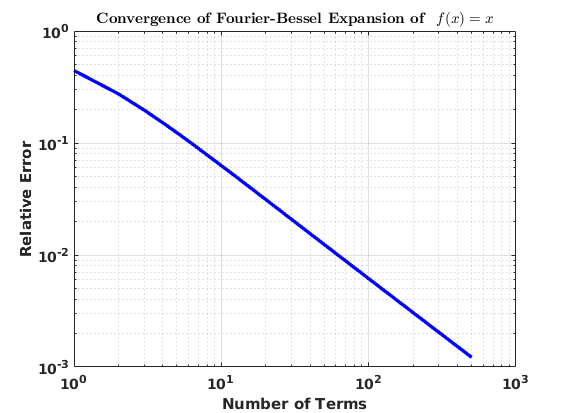
\includegraphics{lec19_ex1_converge.png}
\caption{Convergence of the Fourier-Bessel expansion of $f(x)=x$.}
\label{fig:lec19-converge}
\end{marginfigure}
MATLAB code for quantitatively measuring the relative error as the number of terms increases is shown below.  From Figure \ref{fig:lec19-converge} we can see that, as expected, the relative error steadily goes down.\sidenote{Note that it is conventional to show convergence graphs such as this on a log-log plot.  Eventually, we should expect errors in the determination of Bessel function roots and/or errors in carrying out the numeric integration to prevent further reduction in relative error.} 
%\begin{fullwidth}
\begin{lstlisting}[name=lec19-converge,style=myMatlab]
clear
clc
close 'all'

N = 500; % number of eigenvalues
a = 0; b = 3; % bounds of the domain
nu = 1; kind = 1;
k = besselzero(nu,N,kind); % get roots
alpha = k/b;

f = @(x) x; 
cn = nan(N,1); % store the coefficients (optional)
rel_err = nan(N,1); 

FB = @(x) 0; % initialize the Fourier-Bessel expansion
for n = 1:N
    % compute the i-th coefficient
    cn(n) =...
        integral(@(x) f(x).*besselj(nu,alpha(n)*x).*x,a,b)./...
        integral(@(x) x.*besselj(nu,alpha(n)*x).^2,a,b);
    % update the Fourier-Bessel expansion
    FB = @(x) FB(x) + cn(n)*besselj(nu,alpha(n)*x);

    % calculate sqruare norm of the relative "error"
    err_fn = @(x) FB(x) - f(x); 
    rel_err(n) = integral(@(x) err_fn(x).^2,a,b)./...
        integral(@(x) f(x).^2,a,b); 
end

figure(1)
loglog(1:N,rel_err,'-b',...
    'LineWidth',3);
title('\textbf{Convergence of Fourier-Bessel Expansion of } $$f(x)=x$$',...
    'Interpreter','latex');
ylabel('Relative Error','FontSize',14,...
    'FontWeight','bold');
xlabel('Number of Terms','FontSize',14,...
    'FontWeight','bold');
grid on
set(gca,'FontSize',12,'FontWeight','bold');
\end{lstlisting}
%\end{fullwidth}



\chapter{Lecture 20 - Fourier-Legendre Series Expansion}
\label{ch:lec20}
\section{Objectives}
\begin{itemize}
\item Revisit the Legendre equation as a Sturm-Liouville problem and give its orthogonality relation.
\item Give an example to show the expansion of a function in terms of Legendre polynomials.
\end{itemize}
\setcounter{lstannotation}{0} %hack to try and re-set annotation counter.
\section{Orthogonality with Legendre Polynomials}
We have some experience with Legendre's equation and their solutions, Legendre polynomials.  As a recap, however, Legendre's equation is shown in Equation \ref{eq:lec20-legendre-eq}.
\begin{equation}
\left(1-x^2\right)u^{\prime \prime} - 2xu^{\prime} + n(n+1)u = 0, \ \ x \in (-1,1)
\label{eq:lec20-legendre-eq}
\end{equation}
The general solution is $u(x) = c_nP_n(x)$ where $P_n(x)$ is the Legendre polynomial of order $n$.\marginnote{As a reminder the first few Legendre polynomials are: $P_0(x) = 1$, $P_1(x) = x$, $P_2(x) = \frac{1}{2}\left(3x^2-1\right)$, and $P_3(x) = \frac{1}{2}\left(5x^3-3x\right)$.}  

As demonstrated in Lecture 18, the self-adjoint form for Legendre's equation is given in Equation \ref{eq:lec20-legendre-sa}.
\begin{equation}
\frac{d}{dx}\left[\left(1-x^2 \right) u^{\prime} \right] + \overbrace{n(n+1)}^{\lambda}u = 0
\label{eq:lec20-legendre-sa}
\end{equation}
The orthogonality relation is shown below:\marginnote[1.0cm]{Recall that for Legendre's equation, the weight function $p(x)$ is equal to 1. Also recall that $\left(P_n,P_n \right) = \sfrac{2}{2n+1}$.}
\begin{equation*}
\int_{-1}^{1} P_m(x)P_n(x) (1) \ dx = 
\begin{cases}
0, & m\ne n \\
\frac{2}{2n+1}, & m=n
\end{cases}
\end{equation*}
If we need to represent a function $f(x)$ in terms of Legendre polynomials, we can carry out a \emph{Fourier-Legendre} expansion as shown below:\marginnote[1.0cm]{As usual we can derive the formulas for the coefficients $c_n$ of Equation \ref{eq:lec20-FL-coeff} by multiplying both sides of Equation \ref{eq:lec20-FL-exp} by $P_n(x)$ and integrating.}
\begin{align}
f(x) &= \sum\limits_{n=0}^{\infty}c_n P_n(x) \label{eq:lec20-FL-exp}\\ 
\text{where:}& \nonumber \\
c_n &= \frac{\left(f(x),P_n(x) \right)}{\left(P_n(x),P_n(x) \right)} = \frac{\int_{-1}^{1} f(x) P_n(x) \ dx}{\sfrac{2}{2n+1}} 
\label{eq:lec20-FL-coeff}
\end{align}

The convergence behavior of Fourier-Legendre series expansions is similar to that for the Fourier series expansion using trigonometric polynomials.  This behavior is recapitulated in the next theorem.\marginnote[1.0cm]{This also happens to be true for Fourier-Bessel expansions.} 

\begin{theorem}[Convergence of Fourier-Legendre Series]
Let $f(x)$ and $f^{\prime}(x)$ be piece-wise continuous on the interval $[-1,1]$. Then for all $x$ in the interval, the Fourier-Legendre series of $f$ converges to $f(x)$ at a point where $f(x)$ is continuous and to the average:
\begin{equation*}
\frac{f(x^+) + f(x^-) }{2}
\end{equation*}
at points where $f(x)$ is discontinuous.
\end{theorem}

\vspace{0.5cm}

\noindent\textbf{Example:} Construct the Fourier-Legendre expansion of:
\begin{equation*}
f(x) = 
\begin{cases}
0, & -1 < x < 0 \\
1, & 0 \le x < 1
\end{cases}
\end{equation*}

Since the tools we need to use have largely be introduced already, I will simply present the necessary MATLAB code in a single listing.
\marginnote[2.5cm]{
\ref{lst:ann20-1} Recall that $P_0(x) = 1$ and, according to our formula, 
\begin{align*}
\left(P_0(x),P_0(x)\right) &= \frac{2}{2n+1} \\
  &= \frac{2}{2(0)+1} \\
  &= 2.
\end{align*}
Hence:
\begin{align*}
c_0 &= \frac{\left(f(x),P_0\right)}{\left(P_0,P_0\right)} \\
&= \frac{\int_{-1}^1 f(x) (1) \ dx}{2}
\end{align*}
}
\marginnote[0.5cm]{
\ref{lst:ann20-2} In addition to using the formula for $\left(P_n(x),P_n(x)\right)$ we use the built-in MATLAB function for constructing $P_n(x)$: \lstinline[style=myMatlab]{legendreP(n,x)}.
}
\begin{lstlisting}[name=lec20_ex, style=myMatlab]
clear
clc
close 'all'

f = @(x) ex1(x);

N = 15; % number of terms 
a = -1; b = 1; % boundaries

% handle Po coefficient separately
c0 = (1/2)*integral(@(x) f(x),a,b);  /*!\annotation{lst:ann20-1}!*/
cn = nan(N-1,1);
error_norm = nan(N,1); 

FL = @(x) c0;

% calculate relative error
err_fn = @(x) FL(x) - f(x);
error_norm(1) = integral(@(x) err_fn(x).^2,a,b)./...
        integral(@(x) f(x).^2,a,b); 

for n = 1:(N-1)
    % compute the n'th coefficient /*!\annotation{lst:ann20-2}!*/
    cn(n) = ((2*n+1)/2)*integral(@(x) f(x).*legendreP(n,x),a,b); 
    FL = @(x) FL(x) + cn(n)*legendreP(n,x); %update the expansion
    
    % compute the error.
    err_fn = @(x) FL(x) - f(x);
    error_norm(n+1) = integral(@(x) err_fn(x).^2,a,b)./...
        integral(@(x) f(x).^2,a,b); % normalize error by size of function.
end

%% Plot the result
Nx = 1000;
X = linspace(a,b,Nx);

figure(1)
plot(X,FL(X),'-g',...
    X,f(X),'--b',...
    'LineWidth',3);
grid on
xlabel('X','fontsize',14,'fontweight','bold');
ylabel('f(X)','fontsize',14,'fontweight','bold');
titlestr = ...
    sprintf('Fourier-Legendre expansion, N = %d',N);
title(titlestr,'fontsize',16,'fontweight','bold');
set(gca,'fontsize',12,'fontweight','bold');

%% Plot the error
figure(2)
loglog(1:N,error_norm,'-ok','linewidth',3);
title('Convergence behavior','fontsize',16,'fontweight','bold');
grid on
xlabel('Number of Fourier-Legendre Terms','fontsize',14,'fontweight','bold');
ylabel('Relative Error','fontsize',14,'fontweight','bold');
set(gca,'fontsize',12,'fontweight','bold');


%% Local functions
function y = ex1(x)
[m,n] = size(x); 
% expect vector inputs.
assert(min(m,n) == 1,'Bad input for ex1');  /*!\annotation{lst:ann20-3}!*/
% construct y so that it has the same shape as x
y = nan(m,n); 
for i = 1:length(x) 
    if (x(i) > -1) && (x(i) < 0) 
        y(i) = 0;
    elseif (x(i) >= 0) && (x(i) < 1)
        y(i) = 1;
    end
end
end
\end{lstlisting}
\marginnote[-4.5cm]{\ref{lst:ann20-3} Here we used an \lstinline[style=myMatlab]{assert()} function to enforce the requirement that inputs to \lstinline[style=myMatlab]{ex1(x)} be scalars or vectors but not a matrix.  Any time you write a piece of code that relies on some kind of assumption---the input $x$ must be a vector, for example---you really should add something like this \lstinline[style=myMatlab]{assert()} function to ensure that your assumption really is true.  For larger software projects this sort of small-scale testing is essential for code reliability and maintainability.}
\begin{marginfigure}
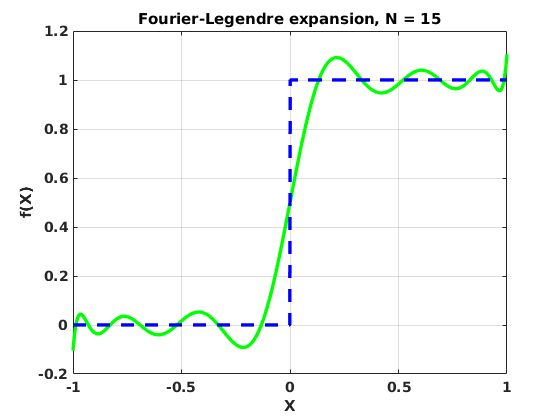
\includegraphics{lec20_ex.png}
\caption{Fourier-Legendre expansion with $N=15$.}
\label{fig:lec20-ex}
\end{marginfigure}

\begin{marginfigure}
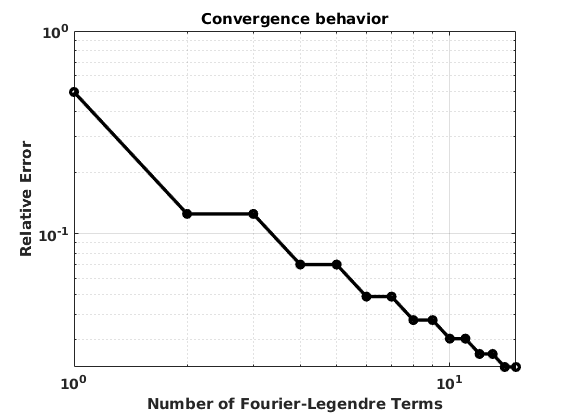
\includegraphics{lec20_converge.png}
\caption{Convergence of Fourier-Legendre expansion}
\label{fig:lec20-conv}
\end{marginfigure}
\newthought{A plot of} the Fourier-Legendre expansion is shown in Figure \ref{fig:lec20-ex} and the convergence behavior is shown in Figure \ref{fig:lec20-conv}.  Several things should be noted.
\begin{enumerate}
\item Clearly we can see from Figure \ref{fig:lec20-ex} that the Fourier-Legendre expansion is converging to the average value at the point of discontinuity at $x=0$.  
\item Like other Fourier expansions, perturbations (``wiggliness'') is introduced by that discontinuity and this is something that we should learn to expect.
\item Also note that from Figure \ref{fig:lec20-conv} we see that the expansion improves when we add the $c_0$ term, the $c_1$ term, $c_3$ term, and all odd-numbered terms but the relative error does not change for the even-numbered terms $c_2,c_4,\dots,c_{14}$.  Looking at $f(x)$ is should be apparent that, in some sense anyway, the function is \emph{odd}---or at least ``odd-ish''; you could make it odd by subtracting out a constant term (i.e. $f(x) - 0.5$ is odd and the $c_0$ coefficient is equal to that 0.5). The even-order Legendre polynomials are even and orthogonal to $f(x)$.  
\end{enumerate}

\chapter{Assignment \#7}
\label{ch:ass7}
\begin{fullwidth}
\noindent Find the eigenfunctions and the equation that defines the eigenvalues for the boundary-value problem.  Use MATLAB to estimate the first 4 eigenvalues $\lambda_1,\lambda_2,\lambda_3,$ and $\lambda_4.$  Give the eigenfunctions corresponding to these eigenvalues and find the square norm of each eigenfunction.

\begin{enumerate}
\item $u^{\prime \prime} + \lambda u = 0, \ \ u^{\prime}(0)=0, \ \ u(1)+u^{\prime}(1) = 0$

\end{enumerate}

\vspace{1.0cm}

\begin{enumerate}[resume]
\item Consider $u^{\prime \prime}+\lambda u = 0$ subject to $u^{\prime}(0)=0, \ u^{\prime}(L)=0$.  Show that the eigenfunctions are:
\begin{equation*}
\left\{ 1, \cos{\frac{\pi x}{L}},\cos{\frac{2\pi x}{L}}, \dots \right\}
\end{equation*}
This set, which is orthogonal on $x\in [0,L]$, is the basis for the Fourier cosine series.
\end{enumerate}

\vspace{1.0cm}

\begin{enumerate}[resume]
\item Consider the following boundary value problem:
\begin{align*}
x^2u^{\prime \prime}+xu^{\prime}+\lambda u &= 0, \ \ x\in(1,5) \\
u(1) = 0, \ \ u(5) &= 0 \\
\end{align*}
\begin{enumerate}
\item Find the (non-trivial) eigenvalues and eigenfunctions of the boundary value problem. Note: this is a Cauchy-Euler equation with solutions of the form $u=x^m$.  

\vspace{0.5cm}

\item Put the differential equation into self-adjoint form.

\vspace{0.5cm}

\item Give the orthogonality relation.  Use MATLAB to verify the orthogonality relation for the first two eigenfunctions.
\end{enumerate}

\end{enumerate}

\vspace{0.75cm}

\begin{enumerate}[resume]
\item Consider Laguerre's differential equation defined on the semi-infinite interval $x \in (0,\infty)$:
\begin{equation*}
xu^{\prime \prime} + (1-x)u^{\prime} + \overbracket{n}^{\lambda} u = 0, \ \ n = 0,1,2,\dots
\end{equation*}
This equation has polynomial solutions $L_{n}(x).$  Put the equation into self-adjoint form and give an orthogonality relation.
\end{enumerate}

\vspace{1.0cm}

\noindent For the next two problems, please use MATLAB along with the provided function \lstinline[style=myMatlab]{besselzero(nu,n,kind)} as shown in class.

\begin{enumerate}[resume]
\item Find the first four $\alpha_n > 0$ defined by $J_1(3\alpha) = 0$.

\vspace{1.0cm}

\item Expand $f(x)=1, \ 0<x<2$, in a Fourier-Bessel series using Bessel functions of order zero that satisfy the boundary condition: $J_0(2\alpha) = 0$.  Make a plot in MATLAB of the given function and the Fourier-Bessel expansion of the function with the first four terms.


\end{enumerate}

\vspace{1.0cm}

\noindent For the next problem, use the MATLAB built-in function \lstinline[style=myMATLAB]{legendreP(n,x)} to represent Legendre Polynomials for Fourier-Legendre expansions.
\begin{enumerate}[resume]
\item Use MATLAB to calculate and print out the value of the first five \underline{non-zero} terms in the Fourier-Legendre expansion of the given function.  Make a plot in MATLAB of the given function and the Fourier-Legendre partial sum with five (non-zero) terms.
\begin{equation*}
f(x) = 
\begin{cases}
0, & -1 < x < 0 \\
x, & 0 < x < 1
\end{cases}
\end{equation*}
\end{enumerate}

\end{fullwidth}


\part{Boundary Value Problems in Rectangular Coordinates}
\chapter{Lecture 21 - Introduction to Separable Partial Differential Equations}
\label{ch:lec21}
\section{Objectives}
\begin{itemize}
\item Review description of linear second-order, Partial Differential Equations (PDEs).
\item Introduce a classification scheme for second-order linear PDEs.
\item Illustrate the use of separation of variables to find solutions to some PDEs.
\end{itemize}

\section{Linear Partial Differential Equations}

Consider the linear, second-order, partial differential equation in two independent variables shown in Equation \ref{eq:lin-second-order-pde}:
\begin{equation}
A\frac{\partial^2u}{\partial x^2} + B\frac{\partial^2 u}{\partial x \partial y} + C\frac{\partial^2 u}{\partial y^2} + D \frac{\partial u}{\partial x} + E\frac{\partial u}{\partial y} + Fu = G
\label{eq:lin-second-order-pde}
\end{equation}
where $A\rightarrow G$ are constants or functions of the \emph{independent} variables $x$ and/or $y$ only.\sidenote{If the coefficients are functions of the dependent variable $u$ or any of its partial derivatives, the equation would, of course, be non-linear.}  If $G=0$ then the equation is \emph{homogeneous}, otherwise the equation is \emph{non-homogeneous}.

\section{Classification of Linear 2\textsuperscript{nd}-Order PDEs}
The solution of a PDE is a \emph{function} of two (or more) independent variables that satisfies the PDE and boundary/initial conditions in some region of the space defined by the independent variables.  Some important qualitative features of the solutions can be anticipated by using the following classification scheme for linear second-order PDEs.

\vspace{0.5cm}

\noindent\textbf{Hyperbolic:} $B^2 - 4AC > 0$ 

Hyperbolic differential equations are characteristic of wave-type phenomena.  In the linear homogeneous case, waves travel through the domain without distortion until a boundary is encountered.  We will examine problems such as vibrating strings and membranes that are governed by hyperbolic PDEs and will exhibit this wave-type behavior.
\marginnote[-1.5cm]{There is an important first-order PDE that does not conform to this classification scheme but is considered hyperbolic; a typical example is the scalar linear advection equation:
\begin{equation*}
u_t + a \cdot \nabla u = f(x,y)
\end{equation*}
This equation exhibits similar wave-type behavior.  

A common non-linear variation is:
\begin{equation*}
u_t + \nabla \cdot f(u) = 0
\end{equation*}
where $f(u)$ is called a \emph{flux function}.  This equation plays a role in modeling a variety of physical conservation laws often associated with transport phenomena.  These equations are known for being capable of producing shocks; discontinuities in the solution even when the initial data is smooth.
}

\vspace{0.5cm}

\noindent\textbf{Parabolic:} $B^2-4AC = 0$

Parabolic differential equations are characteristic of \emph{diffusive} phenomena like transient heat conduction.  The time evolution of the solution of these equations typically has a ``smoothing'' behavior.  Even if the initial data is only piece-wise smooth, as time evolves the solution tends to diffuse into a smooth function.  

\vspace{0.5cm}

\noindent\textbf{Elliptic:} $B^2-4AC < 0$

Elliptic differential equations are characteristic of \emph{steady-state} phenomena like static electrical potential and the steady-state heat equation.

\vspace{0.5cm}

\noindent\textbf{Example:}  Classify the following linear partial differential equations.

\begin{enumerate}
\item $3\frac{\partial^2 u}{\partial x^2} = \frac{\partial u}{\partial y} $

\vspace{0.5cm}

\item $\frac{\partial^2 u}{\partial x^2} = \frac{\partial^2 u}{\partial y^2}$

\vspace{0.5cm}

\item $\frac{\partial^2 u}{\partial x^2} + \frac{\partial^2 u}{\partial y^2} = 0$
\end{enumerate}

\section{Separation of Variables}
The basic technique we will use to solve second-order, linear, homogeneous PDEs is called separation of variables.  Once again, I will illustrate this method by way of doing an example.

\vspace{0.25cm}

\noindent\textbf{Example:} use separation of variables to find product solutions of:
\begin{equation}
\frac{\partial^2 u}{\partial x^2} = 4\frac{\partial u}{\partial y}
\label{eq:lec21-ex}
\end{equation}

\noindent\textbf{Step \#1:} Assume a solution can be expressed as a product of functions---one function for each independent variable.  
\begin{equation*}
u(x,y) = F(x)G(y)
\end{equation*}

\vspace{3.5cm}

\noindent\textbf{Step \#2:} Insert the proposed solution into the governing equation.
\marginnote[1.5cm]{Here we will use subscript notation to denote partial derivatives.}
\begin{align*}
\frac{\partial^2}{\partial x^2}\left[F(x)G(y)\right] &= 4 \frac{\partial}{\partial y}\left[F(x)G(y)\right] \\
F_{xx}G &= 4 FG_{y}
\end{align*}

\vspace{0.5cm}

\noindent\textbf{Step \#3:} Separate variables and introduce a separation constant.  In this example we will separate variables by dividing both sides of the equation by $4FG$.

\begin{align*}
\frac{F_{xx} G}{4FG} &= \frac{4FG_y}{4FG} \\
\frac{F_{xx}}{4F} &= \frac{G_y}{G}
\end{align*}
In this last equation, the terms on the left are only a function of $x$; the terms on the right are only a function of $y$.  The left- and right-hand side of the equality must be the same for \emph{all} values of $x$ and $y$.  The only way this can be expected to be true is if \emph{both} sides are equal to a \emph{\underline{constant}}.\marginnote[-1cm]{This bit of reasoning is a key element of separation of variables.}  We will denote this constant: $-\lambda$.\marginnote[1.5cm]{You might wonder why we chose $-\lambda$ rather than $\lambda$.  In honesty there is no good answer to this question; let us chalk it up to a bias towards having a plus-sign in the separated equations.}
\begin{equation*}
\frac{F_{xx}}{4F} = \frac{G_y}{G} = -\lambda 
\end{equation*}
We can now decompose the partial differential equation in two independent variables into two ordinary differential equations:
\begin{align*}
F_{xx} + 4\lambda F &= 0 \\
G_y + \lambda G &= 0
\end{align*}

\vspace{0.5cm}

\noindent\textbf{Step \#4:} Form product solutions for all possible values of $\lambda$.\marginnote{The ``possible values'' of $\lambda$ can be put into three familiar categories: $\lambda$ can be \emph{positive}, \emph{negative}, or \emph{zero}.}

\vspace{0.25cm}

\noindent\underline{$\lambda = 0$}:
\marginnote{Note how in this case and the cases to follow, we will simply write down the general solution to the separated ODEs with little/no to-do over deriving that solution.  By this point in the course you \emph{need} to be able to quickly recognize those equations.  In most cases you should be able to write down the solutions by inspection.}
\begin{align*}
F_{xx} = 0 &\Rightarrow F(x) = c_1 + c_2x \\
G_y = 0 &\Rightarrow G(x) = c_3 \\
& \\
u(x,y) = F(x)G(x) &= \left(c_1 + c_2x\right) c_3 \\
 &= A_1 + B_1 x
\end{align*}

\vspace{0.25cm}

\noindent\underline{$\lambda < 0$}: For this case we will let $\lambda = -\alpha^2, \ \ \alpha > 0$.
\marginnote{We will assume, for this problem, that the $x$-dimension is bounded and thus it is convenient to use the $\cosh{2\alpha x}$ and $\sinh{2 \alpha x}$ form of the solution.  If the domain is unbounded you would use $e^{2 \alpha x}$ and $e^{-2\alpha x}$.  It will be up to you to make this determination.}
\begin{align*}
F_{xx} - 4 \alpha^2 F = 0 &\Rightarrow F(x) = c_1\cosh{2\alpha x} + c_2 \sinh{2\alpha x} \\
G_y - \alpha^2 G = 0 &\Rightarrow G(y) = c_3e^{\alpha^2 y} \\
& \\
u(x,y) = F(x)G(y) &= \left(c_1\cosh{2\alpha x} + c_2 \sinh{2\alpha x}\right) c_3e^{\alpha^2 y} \\
&= \left(A_2 \cosh{2 \alpha x} + B_2 \sinh{2 \alpha x}\right)e^{\alpha^2 y}
\end{align*}

\vspace{0.25cm}

\noindent\underline{$\lambda > 0$}: For this case we will let $\lambda = \alpha^2, \ \ \alpha > 0$.

\begin{align*}
F_{xx} + 4 \alpha^2 F = 0 &\Rightarrow F(x) = c_1 \cos{2\alpha x} + c_2 \sin{2\alpha x} \\
G_{y} + \alpha^2 G = 0 &\Rightarrow G(y) = c_3e^{-\alpha^2 y} \\
& \\
u(x,y) = F(x)G(y) &= \left(c_1 \cos{2\alpha x} + c_2 \sin{2\alpha x} \right)c_3e^{-\alpha^2 y}  \\
&= \left(A_3 \cos{2\alpha x} + B_3 \sin{2\alpha x} \right)e^{-\alpha^2 y}
\end{align*}

\vspace{0.5cm}

\noindent\textbf{Notes:}  
\begin{itemize}
\item There is no assurance that a linear 2\textsuperscript{nd}-order PDE will be separable.  We will spend a lot of time in this course in dealing with equations that happen to be separable.  In reality, many are not, in particular if the problem is non-homogeneous.  It is a good idea to check to see if an equation is homogeneous before launching down the separation-of-variables path.

\item This example is a bit of an anomaly.  We will usually not attempt to find \emph{general} solutions to PDEs, but only \emph{particular} solutions.  Therefore a problem statement will not be fully meaningful without boundary/initial conditions by which we will be able to derive particular solutions.

\item Specific values of $\lambda$ that result in non-trivial solutions will depend on the boundary conditions.

\item Since the PDEs are linear, the \emph{superposition principle} will apply.  That is, if $u_1,u_2,\dots,u_k$ are solutions of a linear homogeneous PDE (including boundary conditions) then a linear combination:\marginnote{In this equation $c_i$ are constants.}
\begin{equation*}
u = c_1 u_1 + c_2 u_2 + \cdots + c_k u_k
\end{equation*}
is also a solution.
\end{itemize}


\chapter{Lecture 22 - Classical PDEs and BVPs}
\label{ch:lec22}
\section{Objectives}
\begin{itemize}
\item Describe three important PDEs: heat equation, wave equation, and Laplace equation.
\item Describe the physical meaning of common boundary conditions.
\item Discuss important modifications to the three equations to incorporate additional physical phenomena.
\end{itemize}

\section{The Heat Equation}
The time-dependent heat equation in one spatial dimension is given in Equation \ref{eq:heat-eq}:
\begin{equation}
\frac{\partial u}{\partial t} = \alpha^2\frac{\partial^2 u}{\partial x^2}, \ \ \alpha > 0, \ \ a<x<b
\label{eq:heat-eq}
\end{equation}
where $\alpha^2$ corresponds to thermal diffusivity which, in turn is given in Equation \ref{eq:thermal-diffusivity}:
\begin{equation}
\alpha^2 = \frac{k}{\rho c_p}
\label{eq:thermal-diffusivity}
\end{equation}
where $k$ is thermal conductivity, $\rho$ is the density, and $c_p$ is the specific heat at constant pressure and the dependent variable $u$ is the temperature.  All of these material properties must be positive for physically meaningful materials and, for the time being at least, we will consider all of these properties to be constant.\sidenote{This is a very important assumption mathematically and it is also untrue for relevant materials.  The thermal conductivity of most materials is temperature dependent as is the density and specific heat.  If we allowed for this bit of realism to slip into our mathematical analysis, however, the differential equation would become nonlinear---$\alpha$ would become a function of the dependent variable $u$---and we would not be able to solve it with methods taught in this class. Tools based on the finite element method such as MOOSE and COMSOL are specifically designed to deal with this sort of nonlinearity.}

\newthought{We will not} delve into the derivation of Equation \ref{eq:heat-eq}; this is left for your class in heat transfer.  Suffice it to say here that the equation is a mathematical expression of conservation of energy.  The following assumptions are incorporated into this expression:
\begin{enumerate}
\item Heat is flowing in one spatial direction only.  This is the reason why the equation is only a function of $x$.  Think of this as heat flowing in a wire.
\item Since heat is assumed to only flow in the $x$-direction, you should assume that the lateral surfaces of this wire are insulated.  
\item We assume that no heat is generated in the domain.
\item We assume that the material is homogeneous.
\item We also assumed a particular relationship between heat flow and the temperature gradient:\marginnote[-2.0cm]{Strictly speaking, Equation \ref{eq:heat-eq-constituitive} should reference an outward-pointing unit-normal vector.  In a more generic case we would express the relationship as:
\begin{equation*}
q = -k \nabla u \cdot \hat{n}
\end{equation*}
where $\hat{n}$ is the outward-pointing unit normal on the surface through which the heat flux flows and, of course, $\nabla u$, is the temperature gradient.  In a one-dimensional problem like this, $\nabla u$ reduces to $\sfrac{\partial u}{\partial x}$.  To get the physics right (or, more specifically, to get the sign of the heat flux correct) for a particular problem, however, one will need to remember the dot-product with the outward-pointing unit normal.
}
\begin{equation}
q = -k\frac{\partial u}{\partial x}
\label{eq:heat-eq-constituitive}
\end{equation}
where $q$ is the \emph{heat flux}.  Relationships such as given in Equation \ref{eq:heat-eq-constituitive} are referred to as \emph{constitutive} relationships.
\end{enumerate}  

\newthought{To be fully} meaningful as an initial boundary value problem (IBVP), Equation \ref{eq:heat-eq} must be accompanied by an initial condition---say an initial temperature profile, $u(x,0) = f(x)$---and two boundary conditions.  We categorize the boundary conditions into three types:

\vspace{0.5cm}

\noindent\textbf{Type 1:} These are also called \emph{Dirichlet boundary conditions}.\sidenote{Named after the German mathematician Peter Gustav Lejeune Dirichlet who was known as a popular instructor at the Prussian Military Academy in the mid 19\textsuperscript{th} century. He is also famous for having first established the convergence proofs that we have cited for Fourier series and he also studied and proved a unique solution for the first boundary value problem.  That, to the best of my knowledge, is why this boundary condition type is named for him.} These conditions apply to the dependent variable itself.  For example:
\begin{equation*}
u(a) = T_a, \ \ u(b) = f(t)
\end{equation*}

\vspace{0.5cm}

\noindent\textbf{Type 2:} These are also called \emph{Neumann} boundary conditions and they apply to the \emph{derivative} of the dependent variable.  For example:
\begin{equation*}
\frac{\partial u}{\partial x}\Bigl|_{x=a} = 0
\end{equation*}
For the heat equation a homogeneous boundary condition of this type would indicate insulation at a boundary.\sidenote{Insulation implies no heat transfer through a surface---i.e. no heat flux.  Since heat flux is proportional to $\nabla u \cdot \hat{n}$ this implies, for one-dimensional problems, that $\sfrac{\partial u}{\partial x} = 0$.}

\vspace{0.5cm}

\noindent\textbf{Type 3:} These are called \emph{mixed} or \emph{Robin} boundary conditions and they apply to \emph{both} the dependent variable and its derivative.  For example:
\begin{equation*}
\frac{\partial u}{\partial x}\Bigl|_{x=b} = -h\left(u(b,t)-u_m\right), \ \ h>0
\end{equation*}
where, in this case, $u_m$ is a constant reference temperature of the surrounding medium and $h$ is a convective heat transfer coefficient.  This boundary condition would correspond to convective heat transfer at the boundary in which the heat flux is proportional ($h$ being the proportionality constant) to the difference in temperature between the boundary surface and the surrounding medium.

\section{Wave Equation}

The wave equation is given by Equation \ref{eq:wave}:
\begin{equation}
\frac{\partial^2 u}{\partial t^2} = \alpha^2 \frac{\partial^2 u}{\partial x^2}, \ \ \alpha>0, \ \ a<x<b
\label{eq:wave}
\end{equation}
where $\alpha^2 = \frac{T}{\rho}$ and $T$ is tension and $\rho$ is density.\sidenote{The variable $\alpha$ is also often referred to as the \emph{wave speed}.}  The dependent variable $u$ refers to lateral displacement of the string and $t$ is time.
\begin{marginfigure}
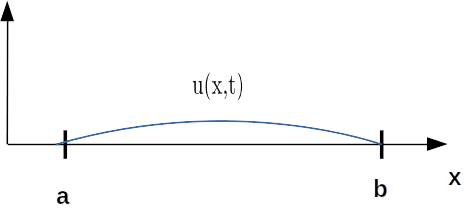
\includegraphics{wave_eq_disp.png}
\end{marginfigure}

This equation is derived as a mathematical expression of mechanical equilibrium of an elastic string held under tension.  The assumptions built-in to this derivation include:
\begin{enumerate}
\item The string is ``perfectly flexible.'' 
\item The string is homogeneous.
\item Displacements in the string are small relative to the string length.
\item Tension is constant; and
\item there are no other forces acting on the string.
\end{enumerate}
A properly stated boundary value problem based on the wave equation will have two boundary conditions.  For this course we will usually apply Dirichlet boundary conditions but others are possible.  Since the equation is second-order in time we also need two temporal boundary conditions.  Typically these are given as the initial displacement, $u(x,0)=f(x)$, and initial velocity, $u_t(x,0)=g(x)$.

\section{Laplace Equation}
The Laplace equation in two dimensions in a Cartesian coordinate system is given by Equation \ref{eq:laplace-eq}:
\begin{equation}
\frac{\partial^2 u}{\partial x^2} + \frac{\partial^2 u}{\partial y^2} = 0
\label{eq:laplace-eq}
\end{equation}
The Laplace equation arises in studies of \emph{steady state} phenomena involving potentials such as: electrostatic potential, gravitational potential, velocity, and heat conduction.  The meaning of the dependent variable $u$, of course, depends upon what is being modeled.  

Equation \ref{eq:laplace-eq} can more concisely and generically be expressed using the Laplace operator $\nabla^2$.\marginnote[-2.0cm]{The Laplace operator $\nabla^2$ is short-hand for:

\begin{equation*}
\nabla^2 = \nabla \cdot \nabla 
\end{equation*}
where in Cartesian coordinates:
\begin{align*}
 \nabla &= \left\langle \frac{\partial}{\partial x}, \frac{\partial}{\partial y}, \frac{\partial}{\partial z} \right\rangle \\
 \nabla \cdot \nabla &= \left\langle \frac{\partial}{\partial x}, \frac{\partial}{\partial y}, \frac{\partial}{\partial z} \right\rangle \cdot \left\langle \frac{\partial}{\partial x}, \frac{\partial}{\partial y}, \frac{\partial}{\partial z} \right\rangle \\
 &= \frac{\partial^2}{\partial x^2} + \frac{\partial^2}{\partial y^2} + \frac{\partial^2}{\partial z^2} \\
&\text{also expressed as: } \\
\nabla^2 &= \bigtriangleup
\end{align*}

}
Using this notation, Equation \ref{eq:laplace-eq} could be written: $\nabla^2 u = 0$.  This same expression is valid for 1-, 2-, or 3-dimensional Cartesian coordinates but it is also valid for polar, cylindrical and spherical coordinates.  The specialization comes in the definition of $\nabla$.  We will address this further when we examine problems in those coordinate systems.

\section{Boundary Value Problems}
In all of the above cases, a full statement of the boundary value problem must include:
\begin{enumerate}
\item The partial differential equation,
\item all boundary conditions, and
\item initial conditions for time-dependent problems.
\end{enumerate}

\vspace{0.5cm}

\noindent\textbf{Example:} Wave Equation Boundary Value Problem.\marginnote{Note that, technically speaking, the PDE does not apply at the domain boundaries or at $t=0$.}
\begin{table}
\begin{tabular}{l l}
PDE & $ \frac{\partial^2 u}{\partial t^2} = \alpha^2 \frac{\partial^2 u}{\partial x^2}, \ \ 0<x<L, \ t>0$\\
 & \\
BCs: & $u(0,t) = 0, \ \ u(L,t) = 0, \ t>0$ \\
 & \\
ICs: & $u(x,0)=f(x), \ \ u_t(x,0)=g(x), \ \ 0<x<L$ \\
\end{tabular}
\end{table}

\subsection{Important Variations to Classic BVPs}
Both the heat equation and the wave equation incorporated several assumptions in the derivation.  If these assumptions are modified or eliminated we can still derive an equation but the form of the equation will change.  Some important variations are described here.

\newthought{In Equation \ref{eq:heat-eq-with-variations}} we show the heat equation in the case where there is an internal heat source and convection from lateral surfaces to a surrounding medium maintained at a constant temperature $u_m$:
\begin{equation}
\frac{\partial u}{\partial t} = \alpha^2 \frac{\partial^2 u}{\partial x^2} \underbrace{+ S(x,t)}_{\text{heat source}} \overbrace{- h(u-u_m)}^{\substack{\text{convection from} \\ \text{lateral surfaces}}}
\label{eq:heat-eq-with-variations}
\end{equation}
where $h$ is the convective heat transfer coefficient.

\newthought{In Equation \ref{eq:wave-eq-with-variations}} we show the wave equation in a case where we have an external force, damping and restoring forces.

\begin{equation}
\frac{\partial^2 u}{\partial t^2} = \alpha^2 \frac{\partial^2 u}{\partial x^2} \overbrace{+f(x,t)}^{\substack{\text{external}\\\text{force}}} \underbrace{-c\frac{\partial u}{\partial t}}_{\text{damping}}\overbrace{-ku}^{\substack{\text{restoring}\\ \text{force}}}
\label{eq:wave-eq-with-variations}
\end{equation}

\vspace{2.0cm}

\newthought{An important skill} that an engineer needs to develop is the ability to translate a description of a physical system into a properly formulated boundary value problem that you can solve.  The \emph{point} is be able to describe a system mathematically so that, by solving the math problem, you gain \emph{insight} into the behavior of the physical system.\marginnote{This is something that students in this class often struggle with.}  Here are a couple of examples to get started.

\vspace{0.15cm}

\noindent\textbf{Example: } Consider a rod of length $L$ that is insulated along its lateral surfaces.  There is heat transfer from the left end of the rod into a surrounding medium at temperature $20^{\circ}$ and the right end is insulated.  The initial temperature is $f(x)$ throughout.  We would like to know what the temperature distribution is as a function of time and space.  The corresponding BVP is:
\begin{table}
\begin{tabular}{l l}
PDE: & $\frac{\partial u}{\partial t}=k\frac{\partial^2 u}{\partial x^2}, \ \ 0<x<L, \ t>0 $ \\
& \\
BCs: & $\frac{\partial u}{\partial x}\Bigl|_{x=0} = -h(u(0,t)-20), \ \  \frac{\partial u}{\partial x}\Bigl|_{x=L} = 0, \ \ t>0$ \\
& \\
IC: & $u(x,0) = f(x), \ \ 0<x<L$ \\
\end{tabular}
\end{table}

\vspace{0.25cm}

\noindent\textbf{Example: } Consider a string of length $L$ held in tension.  The ends are secured to the $x-$axis, and the string is initially at rest on that axis.  An external vertical force proportional to the horizontal distance from the left end acts on the string for $t>0$.  The corresponding BVP is:
\begin{table}
\begin{tabular}{l l}
PDE: & $\frac{\partial^2 u}{\partial t^2} = \alpha^2 \frac{\partial^2 u}{\partial x^2} + hx, \ \ 0<x<L, \ t>0 $ \\
& \\
BCs: & $u(0,t)=0, \ \ u(L,t) = 0, \ t>0 $ \\
& \\
ICs: & $u(x,0) = 0, \ u_t(x,0) = 0, \ \ 0<x<L$ \\
\end{tabular}
\end{table}

\vspace{0.25cm}

\noindent\textbf{Example: } Consider a semi-infinite plate coinciding with the region $0 \le x \le \pi, \ \  y\ge 0.$  The left end is held at temperature $e^{-y}$, and the right end is held at temperature $100^{\circ}$C for $0 < y \le 1$ and $0^{\circ}$C for $y>1$.  The bottom of the plate, $y=0$, is held at temperature $f(x)$.  The corresponding BVP is:

\begin{table}
\begin{tabular}{l l}
PDE: & $\frac{\partial^2 u}{\partial x^2} + \frac{\partial^2 u}{\partial y^2} = 0, \ \ 0<x<\pi, \ y>0 $ \\
& \\
BCs: & $u(0,y) = e^{-y}, \ y>0, \ \ u(\pi,y) = \begin{cases} 100 & 0 < y \le 1 \\ 0 & y>1 \end{cases} $ \\
& $u(x,0) = f(x), \ \ 0<x<\pi $\\
\end{tabular}
\end{table}
One implicit constraint that may need to be applied in this cases is: $\lim_{y \to \infty} u(x,y) < \infty$. 

\chapter{Assignment \#8}
\label{ch:ass8}
\begin{fullwidth}
Use separation of variables to find, if possible, product solutions for the given partial differential equations.  Be sure to consider cases for all possible values of the separation constant.

\begin{enumerate}
\item $\frac{\partial u}{\partial x} = \frac{\partial u}{\partial y}$

\vspace{1.0cm}

\item $\alpha^2 \frac{\partial^2 u}{\partial x^2} - u = \frac{\partial u}{\partial t}, \ \alpha>0$

Note: for this problem, when separating variables, divide by $\alpha^2 X(x)T(t)$ and keep all terms with $\alpha^2$ together.
\end{enumerate}

\vspace{1.0cm}

\noindent Classify the given partial differential equation as hyperbolic, parabolic, or elliptic.
\begin{enumerate}[resume]
\item $\frac{\partial^2 u}{\partial x^2} + \frac{\partial^2 u}{\partial x \partial y} + \frac{\partial^2 u}{\partial y^2} = 0$

\vspace{1.0cm}

\item $\frac{\partial^2 u}{\partial x^2}=0\frac{\partial^2 u}{\partial x \partial y}$

\vspace{1.0cm}

\item $\frac{\partial^2 u}{\partial x^2} + 2 \frac{\partial^2 u}{\partial x \partial y} + \frac{\partial^2 u}{\partial y^2} + \frac{\partial u}{\partial x} - 6 \frac{\partial u}{\partial y} = 0$
\end{enumerate}

\vspace{1.0cm}

\noindent Show that the given partial differential equation possesses the indicated product solution.
\begin{enumerate}[resume]
\item $\frac{\partial u}{\partial t} = k\left(\frac{\partial^2 u}{\partial r^2} + \frac{1}{r} \frac{\partial u}{\partial r} \right)$, $ \ \ u(r,t) = e^{-k \alpha^2 t}\left(c_1 J_0(\alpha r) + c_2 Y_0(\alpha r) \right)$ 

\end{enumerate}

\vspace{1.0cm}

\noindent For the following problems, a rod of length $L$ coincides with the interval $[0,L]$ on the x-axis.  Set up the boundary-value problem for the temperature $u(x,t)$.

\begin{enumerate}[resume]
\item The left end is held at temperature zero and the right end is insulated.  The initial temperature is $f(x)$ throughout.

\vspace{1.0cm}

\item The left end is at temperature $\sin{\left(\sfrac{\pi t}{L} \right)}$, the right end is held at zero, and there is heat transfer from the lateral surface of the rod into the surrounding medium held at temperature zero.  The initial temperature is $f(x)$ throughout.
\end{enumerate}

\vspace{1.0cm}

\noindent For the following problems a string of length $L$ coincides with the interval $[0,L]$ on the x-axis.  Set up the boundary-value problem for the displacement $u(x,t)$.

\begin{enumerate}[resume]
\item The ends are secured to the x-axis. The string is released from rest from the initial displacement $u(x,0) = x(L-x)$.  

\vspace{1.0cm}

\item The left end is secured to the x-axis but the right end moves in a transverse manner according to $\sin{(\pi t)}$.  The string is released from rest from the initial displacement $f(x)$.  For $t>0$ the transverse vibrations are damped with a force proportional to the transverse velocity of the string.
\end{enumerate}


\vspace{1.0cm}

\noindent For the next problem, set up the boundary-value problem for a steady-state temperature $u(x,y)$. 

\begin{enumerate}[resume]
\item A thin rectangular plate coincides with the region in the xy-plane defined by: $0\le x \le 4, \ \ 0 \le y \le 2$.  The left end and the bottom of the plate are insulated.  The top of the plate is held at temperature zero, and the right end of the plate is held at a temperature $f(y)$. 
\end{enumerate}

\end{fullwidth}

\chapter{Lecture 23 - The Heat Equation}
\label{ch:lec23}
\section{Objectives}
\begin{itemize}
\item Demonstrate use of separation of variables to solve the heat equation.
\item Show the code for a MATLAB implementation of an example problem.
\end{itemize}
\section{Analytic Solution}
Consider the following boundary value problem based on the heat equation:
\marginnote[1.0cm]{This boundary value problem models transient heat conduction in a one-dimensional bar.  The ends of the bar are held at a constant temperature of zero degrees and there is an initial temperature distribution described by $f(x)$.}
\begin{table}
\begin{tabular}{l l}
$\substack{\text{Governing} \\\text{Equation}}: $& $\frac{\partial u}{\partial t} = \alpha^2 \frac{\partial^2 u}{\partial x^2}, \ \ \alpha>0, \ \ 0<x<L, \ \ t>0$ \\
& \\
$\substack{\text{Boundary} \\ \text{Conditions}}: $& $u(0,t)=0, \ \ u(L,t) = 0, \ \ t>0$\\
& \\
$\substack{\text{Initial} \\ \text{Conditions}}: $ & $u(x,0) = f(x), \ \ 0<x<L $ \\
\end{tabular}
\end{table}

\vspace{0.25cm}

\noindent We will follow the steps to find the solution using separation of variables.

\vspace{0.5cm}

\noindent\textbf{Step \#1:} Assume a product solution:
\begin{equation*}
u(x,t) = F(x)G(t)
\end{equation*}

\vspace{0.5cm}

\noindent\textbf{Step \#2:} Insert proposed solution into the governing equation:\marginnote{\textbf{Note:} once again we will use subscripts to denote partial derivatives.}
\begin{align*}
\frac{\partial}{\partial t}\left[F(x) G(t)\right] &= \alpha^2 \frac{\partial^2 }{\partial x^2}\left[F(x)G(t) \right] \\
FG_{t} &= \alpha^2 F_{xx}G
\end{align*}

\vspace{3.0cm}

\noindent\textbf{Step \#3:} Separate variables: \marginnote{On the middle line we see that $\frac{G_t}{\alpha^2 G}$ is only a function of $y$; $\frac{F_{xx}}{F}$ is only a function of $x$ and yet they must be equal to each other for all values of $x$ and $y$.  The only way this makes sense is if they are both, in fact, constant.  We will denote this constant $-\lambda$.}
\begin{align*}
\frac{FG_t}{\alpha^2 FG} &= \frac{\alpha^2 F_{xx}G}{\alpha^2 FG} \\
\frac{G_t}{\alpha^2 G} &= \frac{F_{xx}}{F} = -\lambda \\
G_{t} + \alpha^2 \lambda G = 0, \ \ & \ \ F_{xx}+\lambda F = 0
\end{align*}

\vspace{0.5cm}



\noindent\textbf{Step \#4:} Apply boundary conditions to determine non-trivial product solution(s).  

\noindent The boundary conditions must be applied to the separated equation for $F(x)$.\sidenote{The only way $G(t)$ can satisfy the homogeneous spatial boundary conditions would be for us to set $G(t)=0$.  Thus the product solution would be $u(x,t)=F(x)G(t) = F(x)(0)=0$.  Obviously a trivial solution, $u(x,t)=0$, is not what we are looking for.}

\begin{equation*}
F_{xx} + \lambda F = 0, \ \ F(0) = 0, \ \ F(L) = 0, \ \ 0<x<L
\end{equation*}

\noindent We need to examine all possible values of $\lambda$.

\vspace{0.25cm}

\noindent\underline{$\lambda = 0$}:

\begin{align*}
F_{xx} &= 0 \\
F(x) &= c_1x + c_2 \\
F(0) &= c_1(0) + c_2 = 0 \\
\Rightarrow & c_2 = 0 \\
F(L) &= c_1(L) = 0 \\
\Rightarrow & c_1 = 0
\end{align*}
Thus we will disregard $\lambda = 0$ since only the trivial solution satisfies the governing equation and boundary conditions in that case.

\vspace{0.25cm}

\noindent\underline{$\lambda < 0$}:  Here we will set $\lambda = -\nu^2, \ \ \nu>0$. \marginnote[1.5cm]{Note again that we use the $\cosh()$ and $\sinh()$ form of the solution since the domain is bounded.}
\begin{align*}
&F_{xx} - \nu^2 F = 0 \\
&F(x) = c_1 \cosh{\nu x} + c_2 \sinh{\nu x} \\
&F(0) = c_1 \cancelto{1}{\cosh{0}} + c_2 \cancelto{0}\sinh{0} \\
&F(0) = c_1 + 0 = 0 \Rightarrow c_1 = 0 \\
&F(L) = c_2 \sinh{\nu L} = 0 \\
\end{align*}
Here we have to recall that $\sinh{x}$ is strictly positive for $x>0$.  Therefore $c_2 = 0$ and, again, only the trivial solution satisfies the governing equation and boundary conditions for the case $\lambda < 0$ so we will discard this possibility.

\vspace{0.25cm}

\noindent\underline{$\lambda > 0$}:  Here we will set $\lambda = \nu^2, \ \ \nu>0$.
\begin{align*}
&F_{xx} + \nu^2 F = 0 \\
&F(x) = c_1 \cos{\nu x} + c_2 \sin{\nu x} \\
&F(0) = c_1 \cancelto{1}\cos{0} + c_2 \cancelto{0}\sin{0} \\
&F(0) = c_1 + 0 = 0 \Rightarrow c_1 = 0 \\
&F(L) = c_2 \sin{\nu L} = 0
\end{align*}
Finally we have something we can work with!  Rather than setting $c_2 = 0$, we can observe that $\sin{\nu L} = 0$ whenever $\nu L = n \pi$, and $n$ is a positive integer.\marginnote[-1.0cm]{Note that we exclude the case where $n=0$ since that implies $\nu L = 0$ but we stipulated that $\nu > 0$.}  Thus there are infinitely many values---which we will designate $\nu_n$---that satisfy the condition: $\nu_n = \sfrac{n \pi}{L}$ with $n\in \mathcal{Z}^{+}$.\sidenote[][]{Traditionally, in mathematical literature, $\mathcal{Z}$ denotes the set of all integers.  The notation $\mathcal{Z}^{+}$ is used here to denote the set of all positive integers.}

\vspace{0.15cm}

\noindent For $\lambda = \nu^2$ we can now also solve the separated equation for $G(t)$:
\begin{align*}
&G_t + \alpha^2 \nu^2 G = 0 \\
&G(t) = c_3 e^{-(\alpha \nu)^2 t}
\end{align*}

\noindent We combine these values of $\nu_n$ with $F(x)$ and $G(x)$---which we will now call eigenfunctions: 

\begin{align*}
\nu^2_n &= \left(\frac{n \pi}{L} \right)^2 \\
F_n(x) &= c_2\sin{\frac{\nu_n x}{L}} = c_2\sin{\frac{n \pi x}{L}} \\
G_n(t) &= c_3e^{-(\alpha \nu_n)^2 t} = c_3 e^{-(\alpha \frac{n \pi}{L})^2 t}
\end{align*}

\noindent Recall that there are an infinite number of eigenfunctions; the solution will be formed by a linear combination of \emph{all} of them.  So our product solution is:\marginnote{Here we implicitly take $c_2$ and $c_3$ from the separated solutions and combine them into $c_n$.}
\begin{equation*}
u(x,t) = F(x)G(t) = \sum\limits_{n=1}^{\infty} c_n \sin{\frac{n \pi x}{L}} e^{-(\alpha \frac{n \pi}{L})^2 t}
\end{equation*}

\vspace{0.5cm}

\noindent\textbf{Step \#5:} Satisfy the initial condition.

\begin{align*}
u(x,0) &= \sum\limits_{n=1}^{\infty}c_n \sin{\frac{n \pi x}{L}} \cancelto{1}{e^{-(\alpha \frac{n \pi}{L})^2 0}} \\
&= \sum\limits_{n=1}^{\infty}c_n \sin{\frac{n \pi x}{L}} = f(x)
\end{align*}
On the left we have an infinite series of eigenfunctions; on the right we have $f(x)$.  Our job is to find the values of $c_n$ so that they are equal.  This is \emph{exactly} the reason why we spent time learning about Fourier series and orthogonal function expansions.  We will multiply both sides by our (orthogonal) eigenfunctions and integrate.

For $c_1$ we will do this explicitly:\marginnote[1.5cm]{The only non-zero term on the left will be the one corresponding to $\sin{\frac{\pi x}{L}}$; all others will be zero due to the orthogonality of the set of functions $\sin{\frac{n \pi x}{L}}$.}
%\begin{fullwidth}
\begin{multline*}
u(x,0) = c_1\int_0^L \sin{\left(\frac{ \pi x}{L}\right)}^2 \ dx + c_2 \cancelto{=0, \ \text{by orthogonality}}{\int_0^L \sin{\frac{ 2\pi x}{L}} \sin{\frac{ \pi x}{L}} \ dx} + \cdots = \cdots \\ \int_0^L f(x) \sin{\frac{ \pi x}{L}} \ dx
\end{multline*}
%\end{fullwidth}
By orthogonality of the eigenfunctions $F_n(x)$ we can find the coefficients, $c_n$, one at a time by using the formula:
\begin{equation}
c_n = \frac{\int_0^L f(x) \sin{\frac{n \pi x}{L}} \ dx}{\int_0^L \sin{\left(\frac{n \pi x}{L}\right)}^2 \ dx}
\label{eq:lec23-ex1-coeff}
\end{equation}
You might recognize Equation \ref{eq:lec23-ex1-coeff}; it is the same as the Sine series expansion given in Lecture 16. In particular the value of $\int_0^L \sin{\sfrac{n \pi x}{L}}^2 \ dx$ is equal to $\sfrac{L}{2}$ so the formula for the coefficients can be stated more concisely as:

\begin{equation*}
c_n = \frac{2}{L} \int_0^L f(x) \sin{\frac{n \pi x}{L}} \ dx
\end{equation*}
In summary, the solution to our boundary value problem is:

\begin{align*}
u(x,t) &= \sum\limits_{n=1}^{\infty} c_n \sin{\frac{n \pi x}{L}}e^{-(\alpha \frac{n \pi}{L})^2 t} \\
c_n &= \frac{2}{L} \int_0^L f(x) \sin{\frac{n \pi x}{L}} \ dx
\end{align*}

\newthought{To get quantitative} information, we need to specify values for the length of the bar $(L)$, the thermal diffusivity $(\alpha)$, and the initial temperature distribution, $f(x)$.  But we can consider some qualitative aspects of the solution before we start computing.\marginnote{Answers:  
\begin{enumerate}
\item Owing to the exponential term in the solution, $u(x,t) \rightarrow 0$ as $t \rightarrow \infty$.

\item Recalling our experience from Fourier series expansions of functions with discontinuities, the representation will be ``wiggly.''

\item Since the heat equation is a parabolic equation characteristic of diffusive phenomena, we expect the solution to ``smooth-out'' over time.  This should jibe with our own personal intuition and experience with heat transfer.
\end{enumerate}

}
\begin{enumerate}

\item What will the temperature profile look like as $t \rightarrow \infty$?

\item What will the solution look like initially if the temperature profile is piece-wise linear with discontinuities in the interval $[0,L]$?

\item What will happen to the solution as time evolves for temperature profiles that are initially discontinuous? 

\end{enumerate}

\vspace{4.0cm}

\section{MATLAB implementation}
To demonstrate the answer to these questions and help build more insight into the behavior of the transient 1-D heat equation, let us define $L$, $\alpha^2$, and $f(x)$, compute and plot the solution.
\setcounter{lstannotation}{0} %hack to try and re-set annotation counter.


\begin{lstlisting}[name=lec23_ex1, style=myMatlab]
clear
clc
close 'all'

%% Set parameters and define eigenfunctions
L = 1; % length of the domain
alpha_sq = 0.1; % thermal diffusivity /*!\annotation{lst:ann23-1-1}!*/

N = 25; % number of terms to the series solution /*!\annotation{lst:ann23-1-2}!*/

F = @(x,n) sin(n.*pi.*x./L); /*!\annotation{lst:ann23-1-3}!*/
G = @(t,n) exp(-((n.*pi./L).^2)*alpha_sq.*t);

f(x) = @(x) x.*(1-x);

\end{lstlisting}
\marginnote[-6.0cm]{

\vspace{0.75cm}

\ref{lst:ann23-1-1} Strictly speaking we should include units for this quantity.  For perspective, the thermal diffusivity of copper at room temperature is approximately 1.20 cm\textsuperscript{2}/s; for steel approximately 0.20 cm\textsuperscript{2}/s; and for adobe brick around 0.003 cm\textsuperscript{2}/s.

\vspace{0.5cm}

\ref{lst:ann23-1-2} We also need to choose the number of Fourier coefficients to calculate; we obviously cannot calculate them all.


\vspace{0.25cm}

\ref{lst:ann23-1-3} Be sure you understand how to define anonymous functions with multiple variables.

}
Note from Figure \ref{fig:lec23-ex1-smooth-ic} that the initial condition is smooth and satisfies the boundary conditions.
\begin{marginfigure}
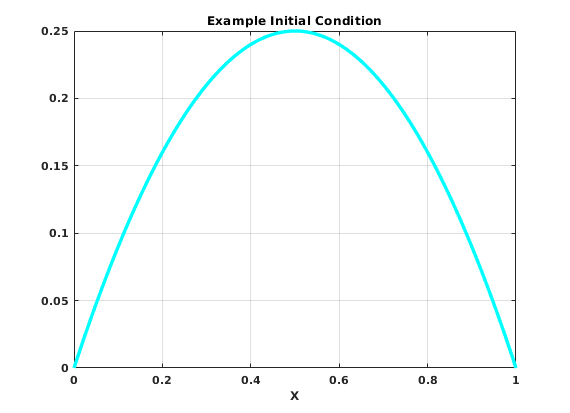
\includegraphics{lec23_ex1_smooth_ic.png}
\caption{Smooth initial condition.}
\label{fig:lec23-ex1-smooth-ic}
\end{marginfigure}

To build the solution we combine the eigenfunctions along with the coefficients calculated using Equation \ref{eq:lec23-ex1-coeff}.

\begin{lstlisting}[name=lec23_ex1, style=myMatlab]
%% Compute the solution
% initialize my series solution
u = @(x,t) 0;
for n = 1:N
    % essentially doing the sine-series half-wave expansion
    % compute the coefficient
    cn = (2/L)*integral(@(x) f(x).*F(x,n),0,L);
    
    % add the term to the series solution
    u = @(x,t) u(x,t) + cn*F(x,n).*G(t,n);
end

%% plot the result
figure(1)
plot(X,u(X,0),'-b',...
    X,u(X,0.1),'-.g',...
    X,u(X,0.5),'--r','linewidth',3);
title_str = sprintf('Heat Equation Example, N=%d',N);
title(title_str,'FontSize',16,'FontWeight','bold');
%title('Lecture #23 Example','fontsize',16,'fontweight','bold');
xlabel('X','fontsize',14,'fontweight','bold');
ylabel('u(X,t)','fontsize',14,'fontweight','bold');
grid on
set(gca,'fontsize',12,'fontweight','bold');
legend('t = 0','t = 0.1','t = 0.5');
\end{lstlisting}
\begin{marginfigure}
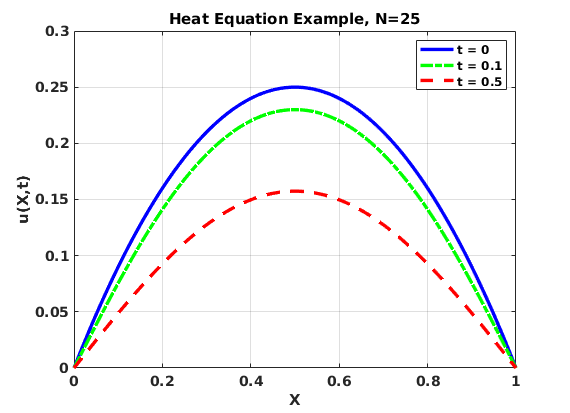
\includegraphics{lec23_ex1_smooth_ic_n25.png}
\caption{Solution for smooth initial condition.}
\label{fig:lec23-ex1-smooth-plot}
\end{marginfigure}
\newthought{The plot is shown} in Figure \ref{fig:lec23-ex1-smooth-plot}. As is expected, the temperature is going down over time. As time goes to infinity, the solution will be zero everywhere.  Recalling that the heat equation is simply a mathematical representation of conservation of energy, you should ask yourself the question: where is the energy going?  The answer is that the energy is flowing out of the left and right side of the bar and will continue to do so as long as the temperature of the bar is higher than the temperature at the boundary which, for this problem, is set to zero.

\newthought{What happens if} we increase the thermal diffusivity?  Answer: the heat flows ``faster.''  Since the thermal diffusivity shows up in the equation $G(t)$, the answer should look like time ``sped up.''  Testing this hypothesis out on our MATLAB solution, we change thermal diffusivity to 1.2.  The results are shown in Figure \ref{fig:lec23-ex1-smooth-plot-copper}.
\begin{marginfigure}
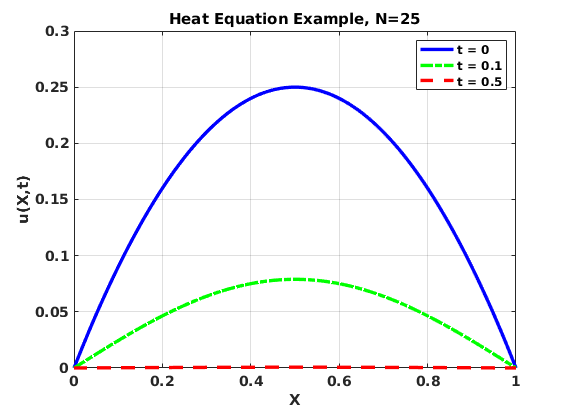
\includegraphics{lec23_ex1_smooth_ic_n25-copper.png}
\caption{Solution with high thermal diffusivity.}
\label{fig:lec23-ex1-smooth-plot-copper}
\end{marginfigure}

\newthought{What happens if} we have a much less smooth initial condition?  Admittedly, it would be odd for the initial temperature distribution to be discontinuous, but given our experience with Fourier series expansions, we should have some idea as to what the Fourier series expansions of discontinuous functions should look like.  To test this, suppose the initial temperature distribution were given by:
\begin{marginfigure}
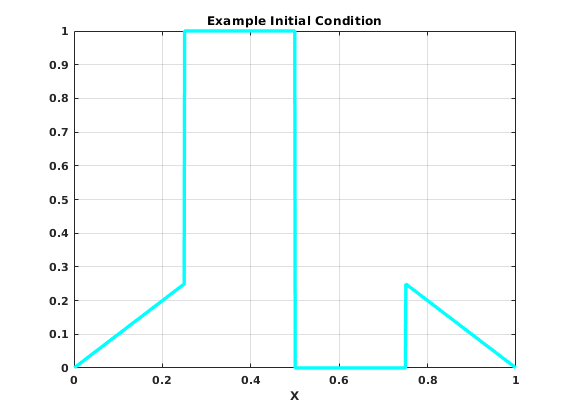
\includegraphics{lec23_ex1_discont_ic.png}
\caption{Example with discontinuous initial condition.}
\label{fig:lec23_ex1_discont}
\end{marginfigure}
\begin{equation*}
f(x) = 
\begin{cases}
x, & 0 < x < \frac{L}{4} \\
1, & \frac{L}{4} \le x < \frac{L}{2} \\
0, & \frac{L}{2} \le x < \frac{3L}{4} \\
L-x, & \frac{3L}{4} \le x < L

\end{cases}
\end{equation*}
and shown in Figure \ref{fig:lec23_ex1_discont}. The solution (for $\alpha^2=0.1$) is shown in Figure \ref{fig:lec23_ex1_discont_n25}. 
\begin{marginfigure} 
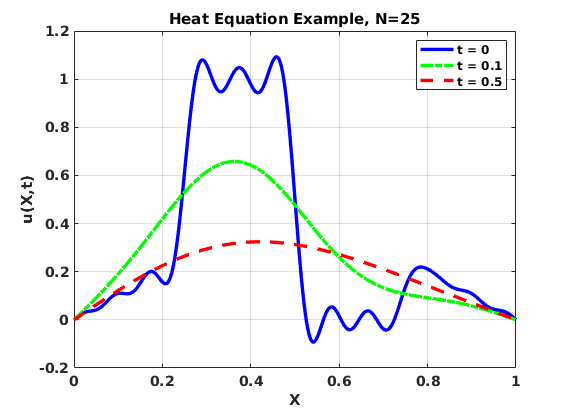
\includegraphics{lec23_ex1_discont_n25.png}
\caption{Solution with discontinuous initial condition, $N=25$.}
\label{fig:lec23_ex1_discont_n25}
\end{marginfigure} 
Note the ``wiggliness'' of the Fourier series representation of the initial condition; note also how that ``wiggliness'' goes away almost immediately. This is due to the diffusive nature of the heat equation.

In much the same way as we could improve our resolution of functions represented by a Fourier series by computing more terms, we can do the same thing here.  In Figure \ref{fig:lec23_ex1_discont_n100} we show the solution computed with $N=100$ terms in the Fourier series.
\begin{marginfigure}
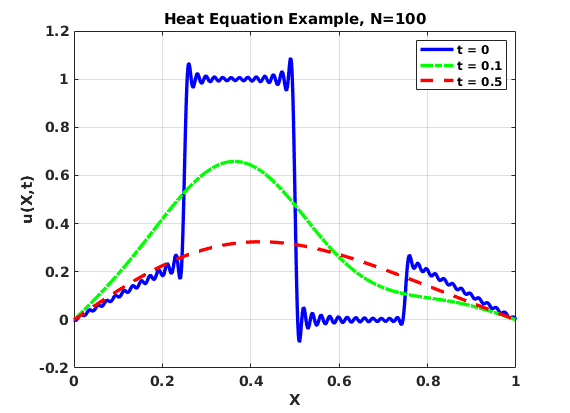
\includegraphics{lec23_ex1_discont_n100.png}
\caption{Solution with discontinuous initial condition, $N=100$.}
\label{fig:lec23_ex1_discont_n100}
\end{marginfigure}

\section{Insulated Boundaries}
%\subsection{One Boundary Insulated}
As an exercise, let us consider what happens when we change the problem by insulating the boundary at $x=L$.  

\begin{table}
\begin{tabular}{l l}
$\substack{\text{Governing} \\\text{Equation}}: $& $\frac{\partial u}{\partial t} = \alpha^2 \frac{\partial^2 u}{\partial x^2}, \ \ \alpha>0, \ \ 0<x<L, \ \ t>0$ \\
& \\
$\substack{\text{Boundary} \\ \text{Conditions}}: $& $u(0,t)=0, \ \ \frac{du}{dx}(L,t) = 0, \ \ t>0$\\
& \\
$\substack{\text{Initial} \\ \text{Conditions}}: $ & $u(x,0) = f(x), \ \ 0<x<L $ \\
\end{tabular}
\end{table}

\vspace{0.25cm}

\noindent Before we do any analysis we should think about what we \emph{expect} the solution to look like.\sidenote{This is important.  Do not let yourself get stuck inside analytic blinders that prevent you from seeing the big picture.  Eventually you will need to be prepared to critically scrutinize your answer and decide, on your own, whether or not it is reasonable and/or correct. To do this, you need to know \emph{in advance} what you \emph{expect} the solution to look like.}  Mathematically we implement the insulated boundary condition by setting the temperature gradient at that boundary equal to zero.  Conceptually, we know this means that heat will no longer flow out of that boundary.  Heat may or may not flow \emph{towards} the right boundary depending on the temperature distribution within the domain but any heat reaching the right boundary will stay there until it can flow out towards the \emph{left} boundary.

\vspace{0.25cm}

\noindent The details are left to the reader\sidenote{\textbf{Hint:} When we apply the insulated boundary condition, we will be left with $F_x(L) = \nu c_2 \cos{\nu L} = 0$ which we can satisfy if $\nu L$ is an odd integer multiple of $\sfrac{\pi}{2}$. So $\nu_n L = \frac{(2n-1) \pi}{2}, \ n=1,2,3,\cdots$, and therefore $\nu_n = \frac{(2n-1)\pi}{2L}$. 
} but application of separation of variables to the new boundary value problem yields the following solution:

\begin{align*}
\nu_n &= \frac{(2n-1)\pi}{2L}, \ \ n=1,2,3,\dots \\
u(x,t) &= \sum\limits_{n=1}^{\infty} c_n \sin{\nu_n x}e^{-(\alpha \nu_n)^2 t} \\
c_n &= \frac{\int_0^L f(x) \sin{\nu_n x} \ dx}{\int_0^L \sin{(\nu_n x)}^2 \ dx}
\end{align*}
A plot of the solution when $N=25$, $L=1$, and $\alpha^2=1.5$ is shown in Figure \ref{fig:lec23-ex2-n25}.

\begin{marginfigure}
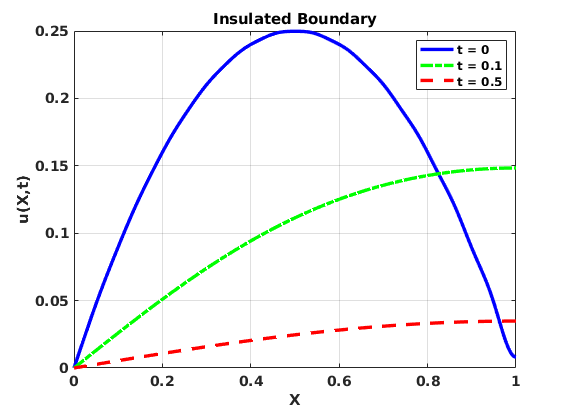
\includegraphics{lec23_ex2_smooth_n25_alphasq1p5.png}
\caption{Solution with an insulated boundary at $x=L$.}
\label{fig:lec23-ex2-n25}
\end{marginfigure}
%\subsection{Both Boundaries Insulated}

\newthought{What happens if} both boundaries are insulated?  Physically, when we insulate something, that means we want to keep heat from coming in or out of the domain.  Does this mean heat will not diffuse \emph{within} the domain?  Of course not; heat will simply flow as it must while driven by temperature gradients in the domain.  When will the diffusion stop?  When there is no more temperature gradient to drive heat flow and that will happen when the temperature is uniform.  

Mathematically, this means that we again change the boundary conditions so that the temperature gradient is zero at \emph{both} boundaries.  The details of this solution will be left to exercises but it is hoped by this point that you already know what the solution \emph{must} look like; namely that heat will diffuse within the domain until a uniform temperature is reached that is equal to the \emph{average} initial temperature.

\chapter{Lecture 24 - The Wave Equation}
\label{ch:lec24}
\section{Objectives}
\begin{itemize}
\item Use separation of variables method to solve the Wave Equation.
\item Illustrate the example solution with MATLAB.
\end{itemize}
\setcounter{lstannotation}{0} %hack to try and re-set annotation counter.

\section{Analytic Solution}
Consider the following boundary value problem based on the wave equation:
\marginnote[1.0cm]{This boundary value problem models a flexible string fixed on both ends with a specified initial displacement, $f(x)$, and initial velocity, $g(x)$.}
\begin{table}
\begin{tabular}{l l}
$\substack{\text{Governing} \\\text{Equation}}: $& $\frac{\partial^2 u}{\partial t^2} = \alpha^2 \frac{\partial^2 u}{\partial x^2}, \ \ \alpha > 0, \ a<x<b$  \\
& \\
$\substack{\text{Boundary} \\ \text{Conditions}}: $& $u(0,t)=0, \ \ u(L,t) = 0, \ \ t>0$\\
& \\
$\substack{\text{Initial} \\ \text{Conditions}}: $ & $u(x,0) = f(x), \ \ u_{t}(x,0) = g(x), \ \ 0<x<L $ \\
\end{tabular}
\end{table}

\vspace{0.25cm}

\noindent We will follow the steps to find the solution using separation of variables.

\vspace{0.5cm}

\noindent\textbf{Step \#1:} Assume a product solution:
\begin{equation*}
u(x,t) = F(x)G(t)
\end{equation*}

\vspace{0.5cm}

\noindent\textbf{Step \#2:} Insert proposed solution into the governing equation:\marginnote{\textbf{Note:} once again we will use subscripts to denote partial derivatives.}
\begin{align*}
\frac{\partial^2}{\partial t^2}\left[F(x) G(t)\right] &= \alpha^2 \frac{\partial^2 }{\partial x^2}\left[F(x)G(t) \right] \\
FG_{tt} &= \alpha^2 F_{xx}G
\end{align*}

\vspace{4.0cm}

\noindent\textbf{Step \#3:} Separate variables: \marginnote{We assume that $F(x)$ and $G(t)$ are not identically zero throughout the domain, thus dividing by $F(x)G(t)$ is mathematically acceptable.}
\begin{align*}
\frac{FG_{tt}}{\alpha^2 FG} &= \frac{\alpha^2 F_{xx}G}{\alpha^2 FG} \\
\frac{G_{tt}}{\alpha^2 G} &= \frac{F_{xx}}{F} = -\lambda \\
G_{tt} + \alpha^2 \lambda G = 0, \ \ & \ \ F_{xx}+\lambda F = 0
\end{align*}
\marginnote[-2.0cm]{On the middle line we see that $\frac{G_{tt}}{\alpha^2 G}$ is only a function of $y$; $\frac{F_{xx}}{F}$ is only a function of $x$ and yet they must be equal to each other for all values of $x$ and $y$.  The only way this makes sense is if they are both in fact constant.  We will denote this constant $-\lambda$.}

\vspace{0.5cm}



\noindent\textbf{Step \#4:} Apply boundary conditions to determine non-trivial product solution(s).  

\noindent The boundary conditions must be applied to the separated equation for $F(x)$.\sidenote{The only way $G(t)$ can satisfy the homogeneous spatial boundary conditions would be for us to set $G(t)=0$.  Thus the product solution would be $u(x,t)=F(x)G(t) = F(x)(0)=0$.  Obviously a trivial solution $u(x,t)=0$ is not what we are looking for.}

\begin{equation*}
F_{xx} + \lambda F = 0, \ \ F(0) = 0, \ \ F(L) = 0, \ \ 0<x<L
\end{equation*}

\noindent We need to examine all possible values of $\lambda$.

\vspace{0.25cm}

\noindent\underline{$\lambda = 0$}:
\marginnote[0.75cm]{This analysis is identical to what we carried out in the last lecture for the heat equation.  It is worth doing this a few times just to make sure you know what you are doing.  After that, you may decide that it is okay to skip to the answer.  Obviously it can be risky to ``skip to the answer'' so do not let me tempt you away from the straight-and-narrow path of always thoroughly looking for valid eigenvalues.}
\begin{align*}
F_{xx} &= 0 \\
F(x) &= c_1x + c_2 \\
F(0) &= c_1(0) + c_2 = 0 \\
\Rightarrow & c_2 = 0 \\
F(L) &= c_1(L) = 0 \\
\Rightarrow & c_1 = 0
\end{align*}
Thus we will disregard $\lambda = 0$ since only the trivial solution satisfies the governing equation and boundary conditions in that case.

\vspace{0.25cm}

\noindent\underline{$\lambda < 0$}:  Here we will set $\lambda = -\nu^2, \ \ \nu>0$. \marginnote[1.5cm]{Note again that we use the $\cosh()$ and $\sinh()$ form of the solution since the domain is bounded.}
\begin{align*}
F_{xx} - \nu^2 F &= 0 \\
F(x) &= c_1 \cosh{\nu x} + c_2 \sinh{\nu x} \\
F(0) &= c_1 \cancelto{1}{\cosh{0}} + c_2 \cancelto{0}\sinh{0} \\
F(0) &= c_1 + 0 = 0 \Rightarrow c_1 = 0 \\
F(L) &= c_2 \sinh{\nu L} = 0 \\
\end{align*}
We once again recall that $\sinh{x}$ is strictly positive for $x>0$.  Therefore $c_2 = 0$ and, again, only the trivial solution satisfies the governing equation and boundary conditions for the case $\lambda < 0$ so we will discard this possibility.

\vspace{0.25cm}

\noindent\underline{$\lambda > 0$}:  Here we will set $\lambda = \nu^2, \ \ \nu>0$.
\begin{align*}
F_{xx} + \nu^2 F &= 0 \\
F(x) &= c_1 \cos{\nu x} + c_2 \sin{\nu x} \\
F(0) &= c_1 \cancelto{1}\cos{0} + c_2 \cancelto{0}\sin{0} \\
F(0) &= c_1 + 0 = 0 \Rightarrow c_1 = 0 \\
F(L) &= c_2 \sin{\nu L} = 0
\end{align*}
Again we see that $\lambda > 0$ works out; our eigenvalues are $\nu_n = \frac{n \pi}{L}$ and eigenfunctions are $F_n(x) = \sin{\frac{n \pi x}{L}}$.  This should not be surprising.  If we have the same separated equation and the same boundary conditions (at least in $x$-direction) we should expect the same eigenvalues and eigenfunctions.

\vspace{0.25cm}

\noindent In this case, the separated equation for $G(t)$ is now:
\begin{align*}
G_{tt} + \alpha^2 \nu^2 G &= 0 \\
G(t) &= c_1 \cos{\alpha \nu t} + c_2 \sin{\alpha \nu t}
\end{align*}



\noindent We combine these values of $\nu_n$ with $F(x)$ and $G(x)$ to get our product solution:
\marginnote{As before, we are combining all of the constants that we can.  Since each solution to $G(t)$ had two unknown constants, we the unknown constant in $F(x)$ into both of them.}
\begin{align*}
u(x,t) = F(x)G(t) &= \sum\limits_{n=1}^{\infty} \left(a_n \cos{\alpha \nu_n t} + b_n \sin{\alpha \nu_n t}\right)\sin{\nu_n t} \\
u(x,t) &= \sum\limits_{n=1}^{\infty} \left(a_n \cos{\alpha \frac{n \pi t}{L}} + b_n \sin{\alpha \frac{n \pi t}{L}} \right) \sin{\alpha \frac{n \pi x}{L}}
\end{align*}

\vspace{0.5cm}

\noindent\textbf{Step \#5:} Satisfy the initial conditions.

\vspace{0.25cm}

\noindent We now have two infinite sets of unknowns: the $a_n$ and $b_n$.  We will resolve these constants through the initial conditions.

\begin{align*}
u(x,0) &= \sum\limits_{n=1}^{\infty} \left(a_n \cancelto{1}{\cos{0}} + b_n \cancelto{0}{\sin{0}} \right)\sin{\alpha \frac{n \pi x}{L}} \\
&= \sum\limits_{n=1}^{\infty} a_n \sin{\alpha \frac{n \pi x}{L}} = f(x)
\end{align*}
Again we find ourselves with an infinite linear combination of orthogonal functions on the left and a function on the right.  Our task is to determine the values of $a_n$ such that they are actually equal.  How do we do this?  We multiply both sides by a member of the set of orthogonal functions and integrate.  This time we will do this explicitly for $a_2$.
\begin{multline*}
a_1 \cancelto{0}{\int_{0}^{L} \sin{\alpha \frac{\pi x}{L}} \sin{\alpha \frac{2 \pi x}{L}} \ dx} + a_2 \int_{0}^{L} \sin{\left(\alpha \frac{2 \pi x}{L}\right)}^2 \ dx + \cdots \text{ all zeros} = \\ \int_{0}^{L} f(x) \sin{\alpha_n \frac{2 \pi x}{L}} \ dx
\end{multline*}
So
\begin{align*}
a_n &= \frac{\int_{0}^{L} f(x) \sin{\alpha_n \frac{n \pi x}{L}} \ dx}{\int_0^L \sin{\left(\alpha \frac{n \pi x}{L} \right)}^2 \ dx} \\
&= \frac{2}{L} \int_{0}^{L} f(x) \sin{\alpha_n \frac{n \pi x}{L}} \ dx
\end{align*}
This defines the values for all $a_n$.  We still need to deal with the $b_n$ so we apply the other boundary condition:

\begin{align*}
u_t(x,0) &= \sum\limits_{n=1}^{\infty}\left(-a_n\alpha \frac{n \pi}{L} \cancelto{0}{\sin{0}} + b_n\alpha \frac{n \pi}{L} \cancelto{1}{\cos{0}} \right) \sin{\alpha \frac{n \pi x}{L}} \\
&=\sum\limits_{n=1}^{\infty} b_n \alpha \frac{n \pi}{L} \sin{\alpha \frac{n \pi x}{L}} = g(x)
\end{align*}
Alas we are in familiar territory now.  To find the values of $b_n$ we need only multiply both sides of the equation by $\sin{\alpha_n \frac{n \pi x}{L}}$ and integrate.\marginnote{Do \textbf{\underline{not}} forget to include the additional constants we gained through taking the derivative of the solution with respect to $t$.}

\begin{align*}
b_n &= \frac{\int_{0}^{L} g(x) \sin{\alpha \frac{n \pi x}{L}} \ dx }{\alpha \frac{n \pi}{L}\int_{0}^{L} \sin{\left(\alpha \frac{n \pi x}{L} \right)}^2} \\
& \\
&= \frac{\int_{0}^{L} g(x) \sin{\alpha \frac{n \pi x}{L}} \ dx }{\alpha \frac{n \pi}{L}\frac{L}{2}} \\
&= \frac{2}{\alpha n \pi} \int_{0}^{L} g(x) \sin{\alpha \frac{n \pi x}{L}} \ dx
\end{align*}  

\vspace{0.25cm}
\noindent In summary, our solution to the wave equation is:
\begin{align*}
u(x,t) &= \sum\limits_{n=1}^{\infty} \left(a_n \cos{\alpha \frac{n \pi t}{L}} + b_n \sin{\alpha \frac{n \pi t}{L}} \right) \sin{\alpha \frac{n \pi x}{L}} \\
a_n &= \frac{2}{L} \int_{0}^{L} f(x) \sin{\alpha_n \frac{n \pi x}{L}} \ dx \\
b_n &= \frac{2}{\alpha n \pi} \int_{0}^{L} g(x) \sin{\alpha \frac{n \pi x}{L}} \ dx
\end{align*}

\vspace{4.0cm}

\section{MATLAB Implementation}
As with the heat equation, we really cannot extract much insight by inspecting the solution formula.  We need to make a plot and to do so we will use MATLAB to represent an approximate solution.\marginnote{For this example we will set the wave speed $\alpha = 1$, the length $L=3$ and the initial conditions as:
\begin{align*}
f(x) &= \begin{cases} \frac{2}{3x}, & 0 < x < \frac{3}{2} \\ \frac{2}{3}(3-x), & \frac{3}{2} \le x < 3 \end{cases} \\
g(x) &= 0
\end{align*}

}
The MATLAB code is given below:
\begin{lstlisting}[name=lec24_ex, style=myMatlab]
clear
clc
close 'all'

%% Example Problem
L = 3;
alpha_sq = 1;% T/rho
alpha = sqrt(alpha_sq);
N = 50;

f = @(x) ex1(x,L);
g = @(x) x.*0;

for n = 1:N
    % compute an
    an = (2/L)*integral(@(x) f(x).*sin(n*pi*x./L),0,L);
    % compute bn
    bn = ...
        (2/(alpha*n*pi))*...
        integral(@(x) g(x).*sin(n*pi*x./L),0,L);
    
    % update the approximate solution
    u = @(x,t) u(x,t) + ...
        (an*cos(alpha.*n*pi*t./L) + ...
        bn*sin(alpha.*n*pi*t./L)).*sin(n*pi*x./L); 
end

%% Fixed Plot, single time step
ts = 3.0;
figure(3)
plot(X,u(X,ts),'-b','Linewidth',3);
title_str = ...
    sprintf('Lecture 24 Example, t = %g',ts);
title(title_str,'fontsize',16,'fontweight','bold');
xlabel('X','fontsize',14,'fontweight','bold');
ylabel('u(X,T)','fontsize',14,'fontweight','bold');
grid on
set(gca,'fontsize',12,'fontweight','bold');
axis([0 L -2.0 2.0]);

%% Local functions
function y = ex1(x,L)
[m,n] = size(x);
y = nan(m,n);
for i = 1:length(x)
   if (x(i)>0)&& (x(i) < L/2)
       y(i) = (2/3).*x(i);
   elseif(x(i) >= L/2) && (x(i)<L)
       y(i) = (2/3)*(L - x(i));
   end
end
end
\end{lstlisting}
The resulting solution is plotted in Figure \ref{fig:lec24-ex1}.
\begin{fullwidth}
\begin{figure}
\subfloat[]{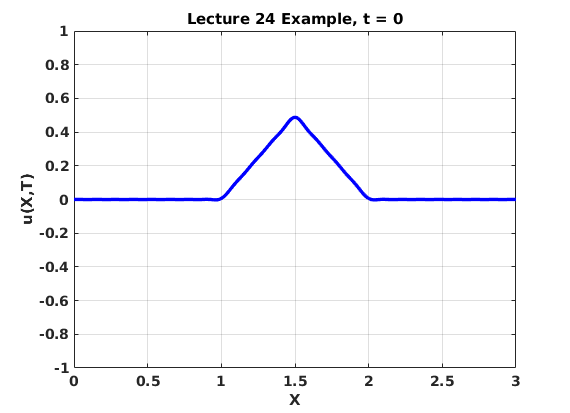
\includegraphics[width=2in]{lec24_t0.png}}
\subfloat[]{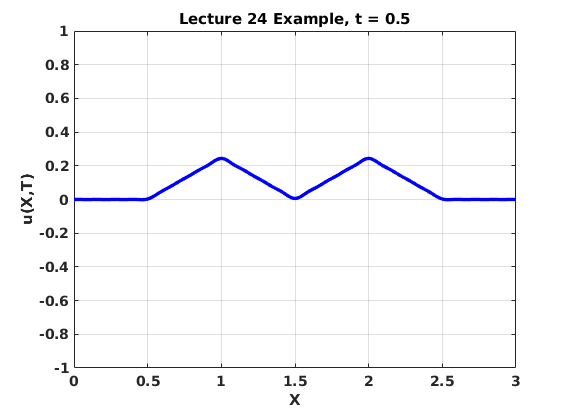
\includegraphics[width=2in]{lec24_t0p5.png}}
\subfloat[]{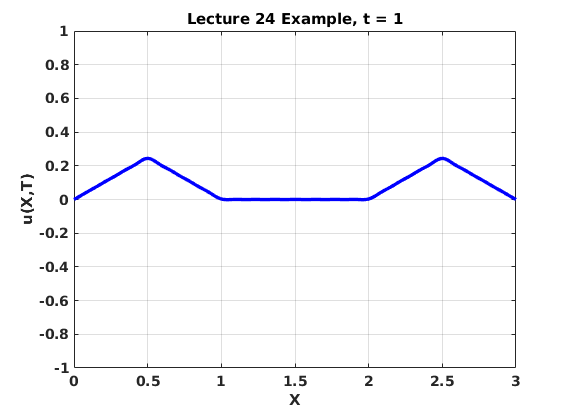
\includegraphics[width=2in]{lec24_t1p0.png}}
\\
\subfloat[]{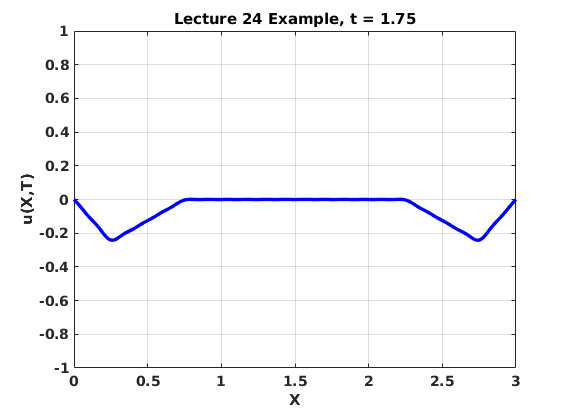
\includegraphics[width=2in]{lec24_t1p75.png}}
\subfloat[]{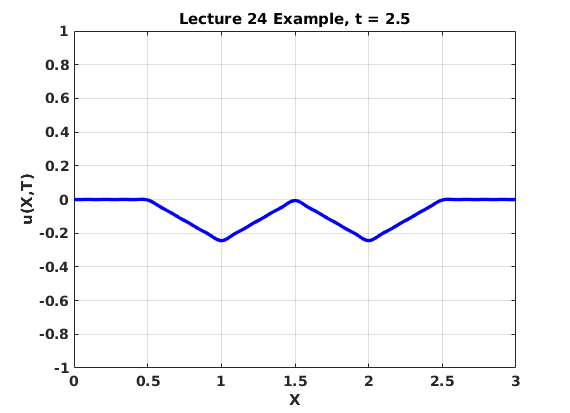
\includegraphics[width=2in]{lec24_t2p5.png}}
\subfloat[]{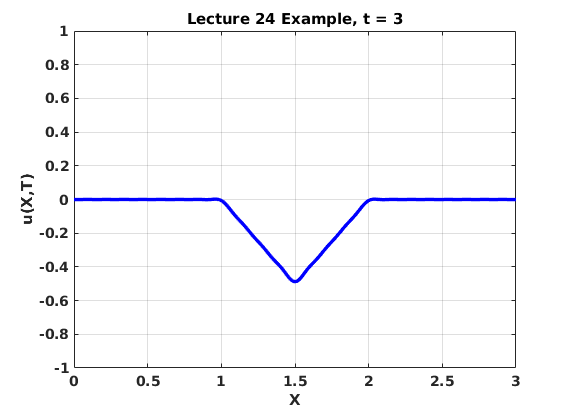
\includegraphics[width=2in]{lec24_t3p0.png}}
\label{fig:lec24-ex1}
\caption[][-1.0cm]{Wave equation solution from $t=0$ to $t=3$ seconds.}
\end{figure}
\end{fullwidth}


\chapter{Lecture 25 - Heat and Wave Equation with MATLAB}
\label{ch:lec25}
\section{Objectives}
\begin{itemize}
\item Describe the details of how to use MATLAB to construct approximate solutions to the heat and wave equations.
\item Illustrate how to create an animation with MATLAB; and
\item show an effective method for creating 2D plots with MATLAB.
\end{itemize}
\setcounter{lstannotation}{0} %hack to try and re-set annotation counter.

\section{Introduction}
In the past two lectures we have invested considerable time in the solution of two boundary value problems using the method of separation of variables.  When I teach this course I find that, during those lectures, there is little time available to spend going into the details of the MATLAB code created, essentially, to visualize the solution. Nonetheless it is often the case that a large fraction of the students have only modest proficiency in using MATLAB.\marginnote{Proficiency levels vary but students have had as much as two years under their belt using MATLAB to as little as two or three weeks.}  In this lecture we focus on the MATLAB details.  The hope is that students will come away with at least an introduction to the bare-minimum of MATLAB tools that will allow them to complete homework assignments.

\section{Example Heat Equation}

\marginnote[-1.0cm]{Take a moment to consider the units used in this boundary value problem.  If you believe the units provided for density, thermal conductivity, and specific heat, simple ``unit arithmetic'' shows that the thermal diffusivity should have units of cm\textsuperscript{2}/s.  What are the units of $\sfrac{\partial^2 u }{\partial x^2}$? Answer: $\sfrac{^{\circ}\text{C}}{\text{cm}^2}$.  What are the units of $\sfrac{\partial u}{\partial t}$?  Answer: $\sfrac{^{\circ}\text{C}}{\text{s}}$.  From this it should be clear that, indeed, the units are the same on the left and right side of the governing equation---as it \emph{must} be in order to be correct.  My point is that it does not take a tremendous amount of mathematical skill to check these things but you should \emph{always} check them.  If you do so, then you will definitely increase your confidence that you know what is going on; you may also save yourself from an embarrassing error.}
\noindent\textbf{Problem Statement: } Find the temperature $u(x,t)$ of a bar of silver of length 10cm.  The density is 10.6 g/cm\textsuperscript{3}, thermal conductivity is 1.04 cal/cm-s-$^{\circ}$C, and the specific heat is 0.056 cal/g-$^{\circ}$C.  The bar is perfectly insulated laterally with ends kept at 0$^{\circ}$C.  The initial temperature, $f(x)$, is given by: $f(x)=4-0.8\left|x-5\right|^{\circ}$C.  From this physical description of the problem, we formulate the following boundary value problem:
\begin{table}[h]
\begin{tabular}{l l}
$\substack{\text{Governing} \\\text{Equation}}: $& $\frac{\partial u}{\partial t} = \alpha^2 \frac{\partial^2 u}{\partial x^2}, \ \ \alpha>0, \ \ 0<x<10, \ \ t>0$ \\
& \\
$\substack{\text{Boundary} \\ \text{Conditions}}: $& $u(0,t)=0, \ \ u(10,t) = 0, \ \ t>0$\\
& \\
$\substack{\text{Initial} \\ \text{Conditions}}: $ & $u(x,0) = f(x) = 4-0.8\left|x-5\right|, \ \ 0<x<10 $ \\
\end{tabular}
\end{table} 

\vspace{4.0cm}

\marginnote[-3.0cm]{Being able to translate this kind of a description of a problem into a properly formulated boundary value problem that you can solve is a key skill you should develop from this course.}



\noindent\textbf{Analytic Solution: } 
\begin{equation}
u(x,t) = \sum\limits_{n=1}^{\infty} c_n \sin{\frac{n \pi x}{10}}e^{-\left(\frac{\alpha n \pi}{10}\right)^2t}
\label{eq:lec25-ex1-sol}
\end{equation}
where $\alpha^2 = \frac{k}{\rho c_p} = \frac{1.04}{(10.6)(0.056)} \text{cm\textsuperscript{2}}/\text{s}$ and the coefficients $c_n$ are given by:
\begin{equation*}
c_n = \frac{2}{10}\int_{0}^{10} \left(4-0.8\left|x-5\right| \right)\sin{\frac{n \pi x}{10}} \ dx
\end{equation*}

\vspace{0.5cm}

\noindent\textbf{MATLAB tasks:}
\begin{enumerate}
\item Construct an approximate representation of the solution in MATLAB including $N=50$ terms of the infinite series.
\item Create a plot of the solution at t = 0, 1, and 10 seconds.
\item Create an animation of the time-dependent temperature profile that you can save and incorporate, for example, in a presentation.
\item Visualize the time-dependent temperature profile using a 2D surface plot.
\end{enumerate}

We will tackle these tasks one at a time.

\vspace{0.25cm}

\noindent\textbf{Task \#1: } Construct an approximate representation of the solution in MATLAB including $N=50$ terms of the infinite series.  

\vspace{0.25cm} 

\noindent In this section of the code we clean out the workspace and provide basic given input data.
\marginnote{ 

\vspace{0.2cm}

\ref{lst:ann25-1-1} It is a good idea to include units and a brief statement indicating what a variable represents.  It may be easy to remember that, for instance, \lstinline[style=myMatlab]{L=10, \% cm} refers to the length but it is less easy to remember that \lstinline[style=myMatlab]{alpha_sq} refers to the thermal diffusivity.

\vspace{0.2cm}

\ref{lst:ann25-1-2} Make sure you fully understand how these anonymous functions work.  The snippet: \lstinline[style=myMatlab]{F = @(x,n) ...} should be read: ``F is a function of x and n...''  The ``L'' that appears on the right hand sides is the same ``L'' defined as a parameter.  The fact that this works is one of the benefits of using anonymous functions.  Remember to write these anonymous functions so that they can accept vector inputs for $x$ and $n$.  Built-in functions like \lstinline[style=myMatlab]{integral()} will fail if the function you supply to be integrated \emph{cannot} accept vector inputs.

}
\begin{lstlisting}[name=lec25-ex1, style=myMatlab]
clear
clc
close 'all'

%% Heat Equation BVP & Solution
L = 10; % cm
alpha_sq = 1.752; % cm^2/s, thermal diffusivity of silver. /*!\annotation{lst:ann25-1-1}!*/

N = 50;

F = @(x,n) sin(n.*pi.*x./L); /*!\annotation{lst:ann25-1-2}!*/
G = @(t,n) exp(-((n.*pi./L).^2)*alpha_sq.*t);

f = @(x) 4 - 0.8*abs(x - 5);

\end{lstlisting}

\vspace{0.25cm}

\noindent Next we will initialize and build---term by term---a truncated version of the infinite series.
\marginnote{

\vspace{0.1cm}

\ref{lst:ann25-1-3} On the surface, this does not do much: it simply creates a variable \lstinline{u} that is a handle to a function of two variables and sets it's initial value to zero.  If we did not have this, however, we would have to create a special case in the \lstinline{for...end} loop to create it on the first trip through.


}
\begin{lstlisting}[name=lec25-ex1, style=myMatlab]
u = @(x,t) 0;/*!\annotation{lst:ann25-1-3}!*/
for n = 1:N
    % essentially doing the sine-series half-wave expansion
    % compute the coefficient
    cn = (2/L)*integral(@(x) f(x).*F(x,n),0,L);
    
    % add the term to the series solution
    u = @(x,t) u(x,t) + cn*F(x,n).*G(t,n);
end
\end{lstlisting}
At this point, our first task is done. The variable \lstinline{u} represents the truncated series solution and we can evaluate the function at any point $x$ or $t$ to get the solution.\sidenote[][-0.75cm]{Sadly, there isn't anything you can do to prevent a user from evaluating the function at invalid/inappropriate vales of $x$ or $t$.  For example, \lstinline{u(1994, -25)} is perfectly legal MATLAB code.}

\vspace{0.25cm}

\noindent\textbf{Task \#2: } Create a plot of the solution at t=0, 1, and 10 seconds. 

\setcounter{lstannotation}{0} %hack to try and re-set annotation counter.
\vspace{0.1cm}

\noindent Code to complete this is presented in the listing below.
\marginnote{

\vspace{0.15cm} 

\ref{lst:ann25-1-4} The \lstinline{\%\%} separates MATLAB code into sections that can be executed independently.  Breaking scripts into sections like this can simplify debugging and helps improve code readability.

\vspace{0.2cm} 

\ref{lst:ann25-1-5} Familiarize yourself with these ``LineSpec'' strings.  For plots with multiple data series you should try to make it easy to tell the difference between different data series even if the plot is viewed in black and white.

\vspace{0.05cm}

\ref{lst:ann25-1-6} Using the \lstinline[style=myMatlab]{'MarkerIndices'} argument allows you to specify which data indices get annotated with a marker (when the line specification includes a marker).  The value \lstinline[style=myMatlab]{1:50:Nx} in this case results in 1 out of every 50 data points having a marker applied.  Experiment with this and see what the plot looks like if you omit this name-value pair.

}
\begin{lstlisting}[name=lec25-ex1, style=myMatlab]
%% Plot the result for fixed times /*!\annotation{lst:ann25-1-4}!*/
% make a discrete X-axis
Nx = 1000;
X = linspace(0,L,Nx);
figure(1)
plot(X,u(X,0),'-ob',...
    X,u(X,1),'-.g',... /*!\annotation{lst:ann25-1-5}!*/
    X,u(X,10),'--r','MarkerIndices',1:50:Nx,'linewidth',3); /*!\annotation{lst:ann25-1-6}!*/
title('Lecture #25 Example','fontsize',16,'fontweight','bold');
xlabel('X [cm]','fontsize',14,'fontweight','bold');
ylabel('u(X,t)   [^{\circ}C]',... /*!\annotation{lst:ann25-1-7}!*/
    'fontsize',14,'fontweight','bold');
grid on
set(gca,'fontsize',12,'fontweight','bold');
legend('t = 0','t = 1','t = 10'); /*!\annotation{lst:ann25-1-8}!*/
\end{lstlisting}

\vspace{0.15cm}

\noindent \ref{lst:ann25-1-7} The string snippet `\string^\{\string\circ \} C' is \LaTeX mark-up and is rendered by MATLAB as $^{\circ}$C.  While not strictly necessary, use of such mark-up can make a plot more attractive.

\vspace{0.15cm}

\noindent \ref{lst:ann25-1-8} Obviously use of a legend makes a plot easier to read.  MATLAB also includes an optional argument named \lstinline{'location'} that can be used with values such as: \lstinline{'northwest','southwest','northeast','southeast','best'}...etc---that allow you to place a legend such that it does not interfere with reading the plot.  Consult the MATLAB documentation for more information about legends.

\vspace{0.15cm}

\noindent A plot created by the code snippet above is shown in Figure \ref{fig:lec25-ex1-plt1}.
\begin{marginfigure}
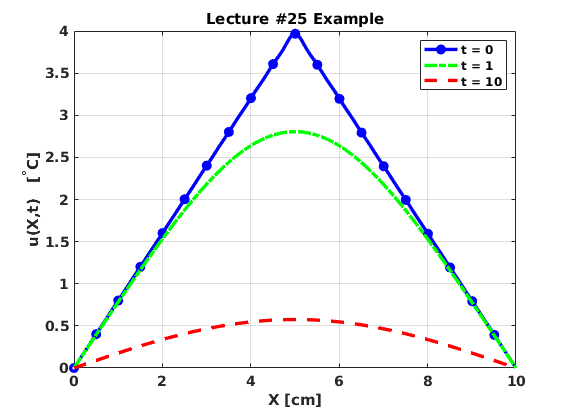
\includegraphics{lec25-ex1-plt1.png}
\caption{Plot of heat equation example at t=0,1, and 10 seconds}
\label{fig:lec25-ex1-plt1}
\end{marginfigure}

\vspace{0.25cm}

\setcounter{lstannotation}{0} %hack to try and re-set annotation counter.
\noindent\textbf{Task \#3: } Create an animation of the time-dependent temperature profile that you can save and incorporate, for example, in a presentation.

\vspace{0.15cm}

\noindent For this task we will first create a simple time-dependent plot that you might use for a homework assignment, independent research project, or for your capstone.  The goal is to gain understanding of the transient behavior of this physical system.

\marginnote{
\vspace{0.25cm}

\ref{lst:ann25-1-9} Discretize time as desired.  

\vspace{0.15cm} 

\ref{lst:ann25-1-10} The \lstinline[style=myMatlab]{sprintf()} allows you to create formatted strings for the title.  In this case, we include the time, in seconds.  The snippet \lstinline[style=myMatlab]{'\%5.3g'} is a formatting string; in this case the value returned from \lstinline[style=MyMatlab]{T(n)} is placed here in a field 5 digits wide with up to 3 digits to the right of the decimal point.  The character `g' tells MATLAB to render the number either in fixed-point notation (e.g. 3.14) or scientific notation (e.g. 1.6e9) whichever is more compact.

\vspace{0.15cm}

\ref{lst:ann25-1-11} This sets the axis limits \lstinline[style=myMatlab]{axis([xmin xmax ymin ymax])}.  The default behavior is to re-scale the plot to fit the max/min plotted values.  For transient simulations this can make changes to the temperature profile harder to understand.  Try running this script without this command to better understand the effect.

}
\begin{lstlisting}[name=lec25-ex1, style=myMatlab]
%% Simple time-dependent plot 
Tmax = 15; % s
NT = 30;
T = linspace(0,Tmax,NT); /*!\annotation{lst:ann25-1-9}!*/
figure(2)
for n = 1:NT
   plot(X,u(X,T(n)),'-b','linewidth',2)
   title_str = sprintf('Lecture #25 Example, t = %5.3g',T(n)); /*!\annotation{lst:ann25-1-10}!*/
   title(title_str,'fontsize',16,'fontweight','bold');
   xlabel('X','fontsize',14,'fontweight','bold');
   ylabel('u(X,T)','fontsize',14,'fontweight','bold');
   grid on
   set(gca,'fontsize',12,'fontweight','bold');
   axis([0 L -0.2 4.5]); /*!\annotation{lst:ann25-1-11}!*/
   pause(Tmax/(NT-1)); /*!\annotation{lst:ann25-1-12}!*/
end
\end{lstlisting}

\vspace{0.15cm}

\ref{lst:ann25-1-12} This command causes MATLAB to pause slightly before starting the next iteration in the for-loop.  The argument to the \lstinline[style=myMatlab]{pause()} function is the duration (in seconds) of the pause.  For some systems this pause also allows the graphics system a chance to update between iterations in the for-loop.  (i.e. if you omit the pause, you may not see your plot update until the very end and miss all of the transient behavior.)

\newthought{This plot is good} for routine homework or analysis that you do not intend to present publicly. Sometimes you \emph{do} want to show a time-dependent plot of a system you are analyzing but you do not want to run the MATLAB script that created the plot during the presentation.  A good option is to create a movie that can be played from most computers and/or can be embedded in a presentation.  The next code block accomplishes this task.
\marginnote{

\vspace{0.3cm}

\ref{lst:ann25-1-13} This creates an array of structures; each structure has two fields, one for the color-data \lstinline{'cdata'}, and one for the color-map \lstinline{'colormap'}. A structure is a data-type that we use infrequently for this course. If you wanted, for instance, to access the 3\textsuperscript{rd} frame color-data you would use the command:

\vspace{0.1cm}

 \lstinline{FRAMES(3).cdata} 

\vspace{1.5cm}

\ref{lst:ann25-1-14} the command \lstinline{gcf} means ``get current frame.''  In this line, the n\textsuperscript{th} frame of the animation is saved to the n\textsuperscript{th} FRAMES structure.

}
\begin{lstlisting}[style=myMatlab, name=lec25-ex1]
%% Save the time-dependent plot as a Movie 
FRAMES(NT) = struct('cdata',[],'colormap',[]); /*!\annotation{lst:ann25-1-13}!*/
figure(3)
for n = 1:NT
    plot(X,u(X,T(n)),'-b','linewidth',3);
    title_str = ...
        sprintf('Lecture #25 Example, t = %g ',T(n));
    title(title_str,'fontsize',16,'fontweight','bold');
    xlabel('X','fontsize',14,'fontweight','bold');
    ylabel('u(X,T)','fontsize',14,'fontweight','bold');
    grid on
    set(gca,'fontsize',12,'fontweight','bold');
    axis([0 L -0.2 4.5]);
    drawnow % ensures graphics pipeline is complete/"flushed"
    FRAMES(n) = getframe(gcf); /*!\annotation{lst:ann25-1-14}!*/
end

%% play the movie
fig = figure(4);
movie(fig,FRAMES,10); % last argument is frames-per-second

%% Write frames to AVI file 
v = VideoWriter('TransientHeat.avi'); /*!\annotation{lst:ann25-1-15}!*/
open(v);
for n = 1:NT
   writeVideo(v,FRAMES(n)); 
end
close(v); /*!\annotation{lst:ann25-1-16}!*/
\end{lstlisting}
\marginnote[-2.5cm]{

\ref{lst:ann25-1-15} This function creates and opens an AVI file to which the \lstinline[style=myMatlab]{writeVideo()} function can write a video frame-by-frame. See MATLAB documentation for other supported video file types.

\vspace{0.15cm}

\ref{lst:ann25-1-16} Be a good citizen and close any files you open for writing. 

}


\vspace{0.25cm}
\setcounter{lstannotation}{0} %hack to try and re-set annotation counter.
\noindent\textbf{Task \#4: } Visualize the time-dependent temperature profile using a 2D surface plot.

\vspace{0.15cm}

\noindent Animations are nice but sometimes the splashy graphics is not needed and you just want to see how the temperature across the domain changes over time in a static image.  A surface plot is an excellent way to do this; the MATLAB built-in function that does the job is cunningly named \lstinline[style=myMatlab]{surf()} and is shown in the listing below.
\marginnote{

\vspace{0.3cm} 

\ref{lst:ann25-1-17} The \lstinline[style=myMatlab]{meshgrid()} function outputs 2D grid coordinates corresponding to the vector inputs for each dimension.  The output arrays \lstinline{XX} and \lstinline{TT} are suitable for use in the \lstinline[style=myMatlab]{surf()} function.

\vspace{0.2cm}



}
\begin{lstlisting}[style=myMatlab, name=lec25-ex1]
%% Plot the temperature vs time in a 2D plot using the surf function
[XX,TT] = meshgrid(X,T); /*!\annotation{lst:ann25-1-17}!*/
figure(5)
surf(XX,TT,u(XX,TT),'edgecolor','none'); /*!\annotation{lst:ann25-1-18}!*/
title('Lecture 25 Suface Plot Example',...
    'fontsize',18,'fontweight','bold');
xlabel('X [cm]','fontsize',16,'fontweight','bold');
ylabel('T [s]','fontsize',16,'fontweight','bold');
zlabel('u(X,T)  [^{\circ}C]','fontsize',16,...
    'fontweight','bold');
\end{lstlisting}

\vspace{0.2cm}

\ref{lst:ann25-1-18} The \lstinline[style=myMatlab]{surf(XX,YY,ZZ)} function takes at least three arguments; in this case the first two are used by the output of \lstinline[style=myMatlab]{meshgrid()} and the last is created by supplying the \lstinline{XX} and \lstinline{TT} arrays to our approximate solution---\lstinline{u(x,y)}---which serves as the height (or z-coordinate) of the surface plot at each point. The name-value pair: \lstinline{'edgecolor','none'} suppresses the (by default) black grid line that delineate the mesh created with \lstinline{XX} and \lstinline{TT}.  For high-resolution meshes the grid lines would obscure the color-map used to highlight the solution. (Try omitting this name-value pair and observe the effect.)

\vspace{0.2cm}

\noindent The resulting surface plot is shown in Figure \ref{fig:lec25-ex1-surf-plt}

\begin{marginfigure}
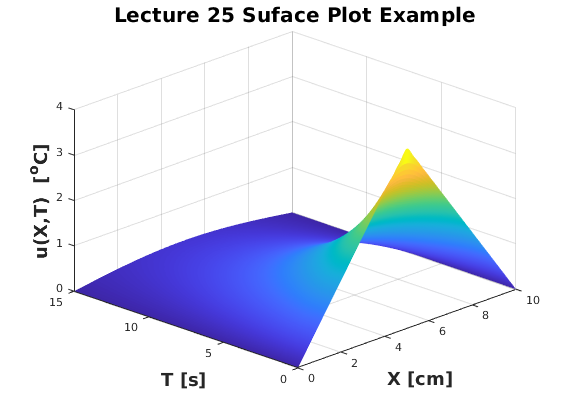
\includegraphics{lec25-ex1-surf-plt.png}
\caption{Surface plot of heat equation example.}
\label{fig:lec25-ex1-surf-plt}
\end{marginfigure}

\section{Example Wave Equation}

For this we will consider the wave equation example analyzed in Lecture 24.  The code may be familiar by this point, but since we did not take the time to go through the MATLAB implementation in detail before, we will take the time here.

\vspace{3.0cm}

\noindent The boundary value problem is given as:
\begin{table}
\begin{tabular}{l l}
$\substack{\text{Governing} \\\text{Equation}}: $& $\frac{\partial^2 u}{\partial t^2} = \alpha^2 \frac{\partial^2 u}{\partial x^2}, \ \ \alpha > 0, \ a<x<b$  \\
& \\
$\substack{\text{Boundary} \\ \text{Conditions}}: $& $u(0,t)=0, \ \ u(L,t) = 0, \ \ t>0$\\
& \\
$\substack{\text{Initial} \\ \text{Conditions}}: $ & $u(x,0) = f(x), \ \ u_{t}(x,0) = g(x), \ \ 0<x<L $ \\
\end{tabular}
\end{table}
where the length is given by $L=3$, wave speed is 1, and the initial conditions are given by:
\begin{align*}
f(x) &= \begin{cases} \frac{2}{3x}, & 0 < x < \frac{3}{2} \\ \frac{2}{3}(3-x), & \frac{3}{2} \le x < 3 \end{cases} \\
g(x) &= 0
\end{align*}

\vspace{0.25cm}
\noindent The analytic solution is:
\begin{align*}
u(x,t) &= \sum\limits_{n=1}^{\infty} \left(a_n \cos{\alpha \frac{n \pi t}{L}} + b_n \sin{\alpha \frac{n \pi t}{L}} \right) \sin{\alpha \frac{n \pi x}{L}} \\
a_n &= \frac{2}{L} \int_{0}^{L} f(x) \sin{\alpha_n \frac{n \pi x}{L}} \ dx \\
b_n &= \frac{2}{\alpha n \pi} \int_{0}^{L} g(x) \sin{\alpha \frac{n \pi x}{L}} \ dx
\end{align*}

\setcounter{lstannotation}{0} %hack to try and re-set annotation counter.

\vspace{0.2cm}

\noindent We begin, again, by cleaning out the workspace and command window and closing all figure windows; then we declare basic problem parameters.
\marginnote{

\vspace{0.5cm}

\ref{lst:ann25-2-1} Recall that $\alpha^2 = \sfrac{T}{\rho}$ where $T$ is the tension (force) and $\rho$ is the density.  Unit analysis shows that $\alpha^2$ has units of: $\sfrac{m \sfrac{L}{t^2}}{\sfrac{m}{L^3}} = \sfrac{L^2}{s^2}$ where $m$ is mass, $L$ is length, and $t$ is time.  Thus $\alpha$ has units of $\sfrac{L}{s}$ and we call it the ``wave speed''.  Now is also a good time to examine the governing equation of the boundary value problem and confirm to yourself that the units make sense.

\vspace{0.2cm}

\ref{lst:ann25-2-2} Notice that the \lstinline{L} from the parameter list is used for the second argument of \lstinline[style=myMatlab]{ex1(x,L)}.  

}
\begin{lstlisting}[name=lec25-ex2, style=myMatlab]
clear
clc
close 'all'

%% Example Problem
L = 3;
alpha_sq = 1;% T/rho
alpha = sqrt(alpha_sq); /*!\annotation{lst:ann25-2-1}!*/
N = 50;

f = @(x) ex1(x,L);/*!\annotation{lst:ann25-2-2}!*/
g = @(x) x.*0; /*!\annotation{lst:ann25-2-3}!*/
\end{lstlisting}
\vspace{0.2cm}

\ref{lst:ann25-2-3} At first glance it would appear to be easier to simply make the assignment: \lstinline[style=myMatlab]{g = 0;}.  We do it this way so that the follow-on code can be written in a way that assumes that \lstinline{g} is a function of $x$---i.e. the code \lstinline[style=myMatlab]{integral(@(x) g(x).*sin(n*pi*x./L,0,L)} does not result in an error. In the future, if we replace $g(x)=0$ with a  non-trivial function of $x$, for example, $g(x)=\sin{x}$ everything will work as expected.

\vspace{3.5cm}

\noindent Next we will initialize our approximate solution and built it up term-by-term.

\begin{lstlisting}[style=myMatlab, name=lec25-ex2]
u = @(x,t) 0;
for n = 1:N
    % compute the coefficients
    an = (2/L)*integral(@(x) f(x).*sin(n*pi*x./L),0,L);
    bn = ...
        (2/(alpha*n*pi))*...
        integral(@(x) g(x).*sin(n*pi*x./L),0,L);
    % update the approximate solution
    u = @(x,t) u(x,t) + ...
        (an*cos(alpha.*n*pi*t./L) + ...
        bn*sin(alpha.*n*pi*t./L)).*sin(n*pi*x./L); 
end
\end{lstlisting}
\marginnote[-3.5cm]{ This equation has two expansion coefficients: $a_n$ and $b_n$, unlike the heat equation which had only one but incorporation of that added complexity in MATLAB is straightforward.
}

\vspace{0.25cm}

\noindent Now that the approximate solution has been computed, we can plot the results.  We may, if we wish, create a dynamic plot much like we did with the heat equation so that we can see the wave behavior in action.

\begin{lstlisting}[style=myMatlab, name=lec25-ex2]
%% make discrete space and time space vectors
Tmax = 3;
NT = 50;
T = linspace(0,Tmax,NT);
Nx = 500;
X = linspace(0,L,Nx);

%% create time-dependent plot
figure(1)
for n = 1:NT
   plot(X,u(X,T(n)),'-b','linewidth',3); 
   title_str = sprintf('Lecture 24 Example, t = %g ',T(n));
   title(title_str,'fontsize',16,'fontweight','bold');
   xlabel('X','fontsize',14,'fontweight','bold');
   ylabel('u(X,T)','fontsize',14,'fontweight','bold');
   grid on
   set(gca,'fontsize',12,'fontweight','bold');
   axis([0 L -1.5 1.5]);
   pause(Tmax/(NT-1));
end
\end{lstlisting}

\vspace{0.25cm}

\noindent Or we can make a single plot with multiple data-series as shown in Figure \ref{fig:lec25-ex2-plt1}:
\begin{marginfigure}
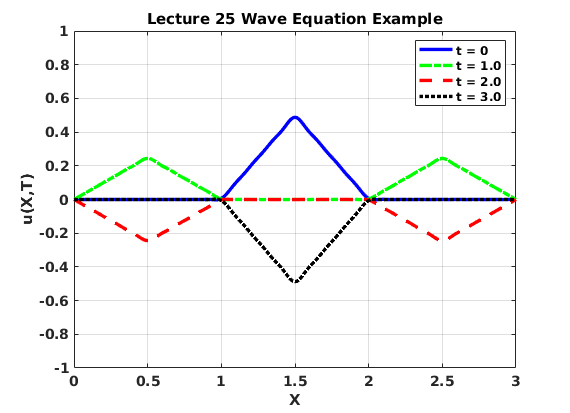
\includegraphics{lec25-ex2-plt1.png}
\caption{Plot of wave equation example problem at t=0, 1.0, 2.0, and 3.0 sec.}
\label{fig:lec25-ex2-plt1}
\end{marginfigure}

\begin{lstlisting}[style=myMatlab, name=lec25-ex2]
%% fixed plot, multiple data series
figure(2)
plot(X,u(X,0),'-b',...
    X,u(X,1.0),'-.g',...
    X,u(X,2.0),'--r',...
    X,u(X,3.0),':k','linewidth',3);
title('Lecture 25 Wave Equation Example',...
    'fontsize',16,'fontweight','bold');
xlabel('X','fontsize',14,'fontweight','bold');
ylabel('u(X,T)','fontsize',14,...
    'fontweight','bold');
grid on
set(gca,'fontsize',12,'fontweight','bold');
axis([0 L -1.0 1.0]);
legend('t = 0','t = 1.0','t = 2.0','t = 3.0',...
    'location','best');
\end{lstlisting}

\vspace{1.0cm}

\noindent Lest we forget, we also need to define the function \lstinline[style=myMatlab]{ex1(x,L)}.  We choose to do this as a \emph{local function} which means that it has to be placed \emph{at the end} of the script file.

\begin{lstlisting}[style=myMatlab, name=lec25-ex2]
%% Local functions
function y = ex1(x,L)
[m,n] = size(x);
y = nan(m,n);
for i = 1:length(x)
   if (x(i)>0)&& (x(i) < L/2)
       y(i) = (2/3).*x(i);
   elseif(x(i) >= L/2) && (x(i)<L)
       y(i) = (2/3)*(L - x(i));
   end
end
end
\end{lstlisting}

\chapter{Assignment \#9}
\label{ch:ass9}
\begin{fullwidth}


\begin{enumerate}
\item Consider the heat equation given in the following boundary value problem:
\begin{table}[h]
\begin{tabular}{l l}
$\substack{\text{Governing} \\\text{Equation}}: $& $\frac{\partial u}{\partial t} = \alpha^2 \frac{\partial^2 u}{\partial x^2}, \ \ \alpha>0, \ \ 0<x<L, \ \ t>0$ \\
& \\
$\substack{\text{Boundary} \\ \text{Conditions}}: $& $u(0,t)=0, \ \ u(L,t) = 0, \ \ t>0$\\
& \\
$\substack{\text{Initial} \\ \text{Conditions}}: $ & $u(x,0) = f(x) = 
\begin{cases}
1, & 0 < x < \sfrac{L}{2} \\
0, & \sfrac{L}{2} \le x < L 
\end{cases}, \ \ 0<x<L $ \\
\end{tabular}
\end{table}

Solve this boundary value problem using separation of variables.  Use MATLAB to represent the solution of this equation for $\alpha^2 = 1$ and $L=1$.  Truncate the series solution at $N=25$ terms.  Plot the solution with separate lines for the solution at t=0, t=0.1, and t=0.5. 


\vspace{2.0cm}

\item Solve the heat equation using separation of variables and find the temperature $u(x,t)$ in a rod of length $L$ with thermal diffusivity $\alpha^2$, if the initial temperature is $f(x)$ throughout and if the ends $x=0$ and $x=L$ are insulated.


\vspace{2.0cm}

\item Suppose heat is lost from the lateral surface of a thin rod of length $L$ into a surrounding medium at temperature zero.  If the linear law of heat transfer applies, then the heat equation takes on the form:

\begin{equation*}
\alpha^2 \frac{\partial^2 u}{\partial x^2} - hu = \frac{\partial u}{\partial t}, \ \ 0<x<L, \ \ t>0
\end{equation*}
where $h$ is a constant.  Use separation of variables and find the temperature $u(x,t)$ if the initial temperature is $f(x)$ throughout and the ends $x=0$ and $x=L$ are insulated. \textbf{Note:} when separating variables, keep $h$ with the time-dependent part of the equation.


\vspace{2.0cm}

\item Solve the heat equation using separation of variables subject to the following boundary and initial conditions:
\begin{align*}
u(0,t) &= 0, \ \ u(100,t) = 0, \ \ t>0 \\
u(x,0) &= 
\begin{cases}
0.8x, & 0 \le x \le 50 \\
0.8(100-x), & 50 < x \le 100
\end{cases}
\end{align*}
Use MATLAB to represent the solution of this equation for $\alpha^2 = 1.6352$ and $L=100$.  Truncate the series solution at $N=25$ terms.  Plot the solution with separate data series for the solution at t=0, t=10, and t=50 seconds.  Create a surface plot (use the MATLAB built-in function \lstinline[style=myMatlab]{surf()} with $0 \le x \le 100$ as one dimension and $0 \le t \le 200$ as the other.

\vspace{2.0cm}

\item Solve the wave equation using separation of variables subject to the given conditions:
\begin{align*}
u(0,t) &= 0, \ \ u(\pi,t)=0, \ \ t>0 \\
u(x,0) &=0, \ \ u_{t}(x,0) = \sin{x}, \ \ 0 < x < \pi
\end{align*}

\vspace{2.0cm}

\item Use separation of variables to solve the wave equation subject to the following conditions:
\begin{align*}
u(0,t) &= 0, \ \ u(1,t)=0, \ \ t>0 \\
u(x,0) &=x(1-x), \ \ u_{t}(x,0) = x(1-x), \ \ 0 < x < 1
\end{align*}
Use MATLAB to represent this solution.  Truncate the series solution at $N=25$ terms.  Make a plot that shows the position $u(x,t)$ for t = 0,1,5, and 10.
\end{enumerate}


\end{fullwidth}

\chapter{Review Problems \#2}
\label{ch:rev2}
\begin{fullwidth}
\section{List of topics}
\begin{enumerate}
\item Orthogonal Functions and Fourier Series
\begin{enumerate}
\item Orthogonal Functions
\item Fourier series
\item Sturm-Liouville eigenvalue problems
\item Fourier-Bessel and Fourier-Legendre expansions
\end{enumerate}

\item Boundary Value Problems in Rectangular Coordinates
\begin{enumerate}
\item Finding product solutions of separable partial differential equations.
\item Classifying partial differential equations.
\item Solving the heat equation and wave equation with various boundary/initial conditions.
\end{enumerate}

\end{enumerate}

\section{Review Problems}

\begin{enumerate}
\item Suppose the function $f(x)=x^2+1, \ \ 0<x<3$, is expanded in a Fourier series, a cosine series, and a sine series.  Draw a sketch of each expansion from $-3<x<3$ and indicate the value to which the expansion converges at $x=0$ in each case.


\vspace{1.0cm}

\item The product of an odd function $f(x)$ with an odd function $g(x)$ is an \rule{2cm}{0.15mm} function.


\vspace{1.0cm}

\item To you were to expand $f(x)=\left|x\right|+1, \ \ -\pi < x < \pi$, in a trigonometric series, the series that would converge most quickly would be a \rule{2cm}{0.15mm} series expansion.

\vspace{1.0cm}

\item Consider Chebyshev's differential equation:
\begin{equation*}
\left(1-x^2\right)u^{\prime \prime} - xu^{\prime}+n^2u=0, \ \ -1 < x < 1
\end{equation*}
which for integer $n=0,1,2,\dots$, have polynomial solutions called Chebyshev polynomials which are denoted $T_n(x)$.  Express Chebyshev's equation in self-adjoint form and write the orthogonality relation for Chebyshev polynomials.

\vspace{1.0cm}

\item Consider a rod of length $L$ coinciding with the interval $[0,L]$ on the x-axis.  Set up the boundary-value problem for the temperature $u(x,t)$ where there is heat transfer from the left end into a surrounding medium which is maintained at a temperature of 20$^{\circ}$, and the right end is insulated.  The initial temperature throughout the rod is $f(x)$. 

\vspace{1.0cm}

\item Solve the wave equation subject to the conditions:
\begin{align*}
u(0,t)&=0, \ \ u(\pi,t) = 0, \ t>0 \\
u(x,0)&=0.01 \sin{3x}, \ \ u_{t}(x,0)=0, \ \ 0<x<\pi
\end{align*}

\vspace{1.0cm}

\item Consider a string of length $L=4$ and $h=1$ fixed at both ends with initial displacement as shown in the sketch below.

\begin{figure}[h!]
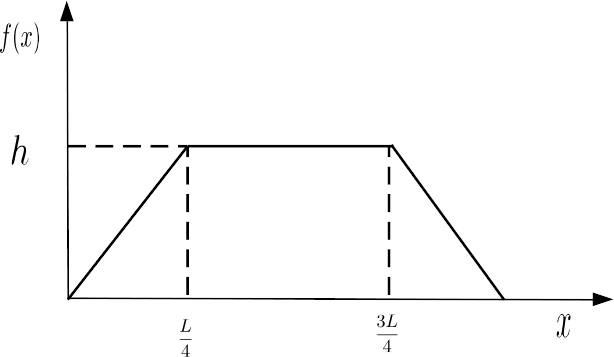
\includegraphics{review2_fig.png}
\end{figure}
Using MATLAB syntax, complete the local function shown in the space below:
\begin{lstlisting}[style=myMatlab, frame=none, numbers=none]
%% Local Function to implement IC
function y = ICfun(x)
[m,n] = size(x);
y = nan(m,n);

for i = 1:length(x)










end
end
\end{lstlisting}

\end{enumerate}

\end{fullwidth}

\chapter{Lecture 26 - Laplace's Equation}
\label{ch:lec26}
\section{Objectives}
\begin{itemize}
\item Solve a boundary value problem based on Laplace's equation representing steady-state temperature in a rectangular domain.
\item Show how to use the superposition principle to solve Laplace's equation with multiple non-homogeneous boundary conditions.
\end{itemize}
\setcounter{lstannotation}{0} %hack to try and re-set annotation counter.

\section{Laplace Equation Example}
Consider the system depicted in Figure \ref{fig:lec26-fig1} and described by the following boundary value problem based on Laplace's Equation.
\begin{marginfigure}
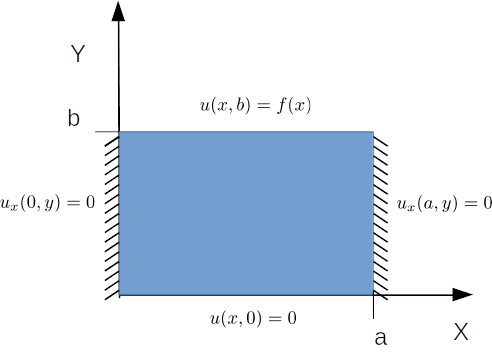
\includegraphics{lec26_fig1.png}
\caption{Schematic of example Laplace's equation problem.}
\label{fig:lec26-fig1}
\end{marginfigure}
\begin{table}[h]
\begin{tabular}{l l}
$\substack{\text{Governing} \\\text{Equation}}: $& $\frac{\partial^2 u}{\partial x^2} + \frac{\partial^2 u}{\partial y^2} = 0, \ \ 0<x<a, \ \ 0<y<b $\\
& \\
$\substack{\text{Boundary} \\ \text{Conditions}}: $ & $\substack{u(x,0)=0  \ \ \ \ \ \ u_x(0,y) = 0 \\ \\ u(x,b) = f(x) \ \ u_x(a,y) = 0}$ 
\end{tabular}
\end{table} 
We will find the solution to this boundary value problem using separation of variables.

\vspace{0.25cm}

\noindent\textbf{Step \#1:} Assume a product solution.
\begin{equation*}
u(x,y) = F(x)G(y)
\end{equation*}

\vspace{0.25cm}

\noindent\textbf{Step \#2:} Insert proposed solution into the governing equation.

\begin{align*}
\frac{\partial^2}{\partial x^2}\left[F(x)G(y)\right] + \frac{\partial^2}{\partial y^2}\left[F(x)G(y)\right] &= 0 \\
F_{xx}G + FG_{yy} &= 0
\end{align*}

\vspace{4.5cm}

\noindent\textbf{Step \#3:} Separate variables by dividing by $F(x)G(y)$:\marginnote{Once again we assume that neither $F(x)$ nor $G(y)$ are identically equal to zero throughout the domain, therefore it is mathematically acceptable for them to appear in the denominator.}
\begin{align*}
\frac{F_{xx}G}{FG} + \frac{FG_{yy}}{FG} &= 0 \\
\frac{F_{xx}}{F} + \frac{G_{yy}}{G} &= 0 \\
\frac{F_{xx}}{F} = -\frac{G_{yy}}{G} &= -\lambda \\
F_{xx}+\lambda F &= 0 \\
G_{yy}-\lambda G &= 0
\end{align*}
This gives us two separated boundary value problems to solve.

\vspace{0.5cm}

\noindent\textbf{Step \#4:} Apply boundary conditions to determine non-trivial product solution(s).
\begin{marginfigure}
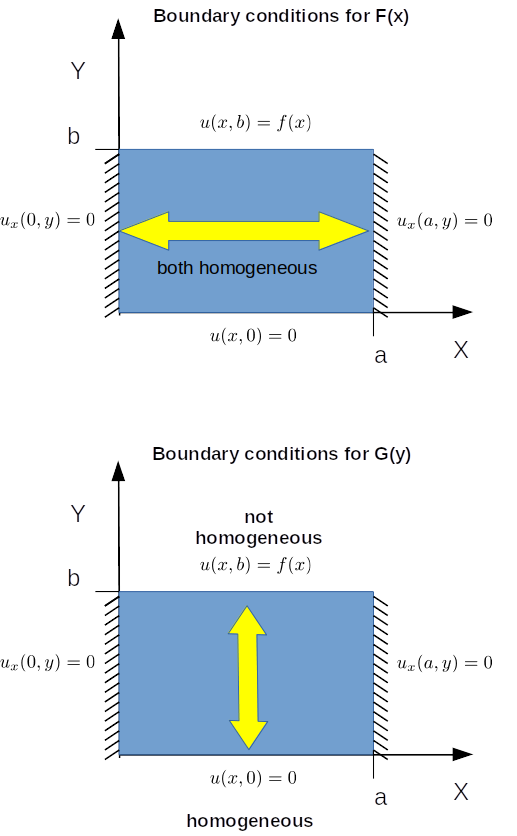
\includegraphics{lec26_bcs.png}
\caption{Pairs of boundary conditions for Laplace's equation.}
\label{fig:lec26-bcs}
\end{marginfigure}

\vspace{0.1cm}

\noindent In order to determine allowable values for $\lambda$, we find solutions to the separated boundary value problem that has \emph{all homogeneous boundary conditions.}\sidenote{If neither separated boundary value problem has all homogeneous boundary conditions, you will need to solve the problem in multiple phases and use the superposition principle to obtain an answer.  This is discussed in the last section of this lecture.}  So we will examine $F_{xx} + \lambda F = 0$.  As usual, we will have to check for all possible values of $\lambda$.

\vspace{0.1cm}

\noindent\underline{$\lambda = 0$}:

\begin{align*}
F_{xx} &= 0 \\
F(x) &= c_1x + c_2 \\
\Rightarrow F_{x} &= c_1 \\
F_x(0) = c_1 &= 0 \\ 
F_{x}(a) &= 0 \ \text{ (satisfied)}
\end{align*}

\vspace{0.1cm}

\noindent We see that, while $c_1$ must be zero, $F(x)=c_2$ satisfies both boundary conditions for any value of $c_2$.  Thus $\lambda = 0$ is an acceptable eigenvalue and the corresponding eigenfunction is a constant.

\vspace{0.1cm}

\noindent\underline{$\lambda < 0$}: To ensure $\lambda$ is negative we will set $\lambda = -\alpha^2, \ \alpha>0$.
\marginnote[1.5cm]{Since the domain is bounded between $0<x<a$, we will use the $\cosh{}$ and $\sinh{}$ form of the solution.}
\begin{align*}
F_{xx} - \alpha^2 F &= 0 \\
F(x) &= c_1 \cosh{\alpha x} + c_2 \sinh{\alpha x} \\
F_x(x) &= \alpha c_1 \sinh{\alpha x} + \alpha c_2 \cosh{\alpha x} \\
F_x(0) &= \alpha c_1 (0) + \alpha c_2 (1) = 0 \\
\Rightarrow c_2 &= 0 \\
F_x(a) &= \alpha c_1 \sinh{a \alpha} = 0\\
\Rightarrow c_1 &= 0
\end{align*}
\marginnote[-1.5cm]{For this last two lines, recall that $\sinh{x}$ is positive for all $x>0$.}
Therefore only the trivial solution $F(x)=0$ satisfies the separated equation and boundary conditions if $\lambda < 0$.

\vspace{0.5cm}

\noindent\underline{$\lambda > 0$}: To insure $\lambda$ is positive we will set $\lambda = \alpha^2, \ \alpha>0$.

\begin{align*}
F_{xx}+\alpha^2 F &= 0 \\
F(x) &= c_1 \cos{\alpha x} + c_2 \sin{\alpha x} \\
F_{x}(x) &= -\alpha c_1 \sin{\alpha x} + \alpha c_2 \cos{\alpha x} \\
F_{x}(0) &= -\alpha c_1 (0) + \alpha c_2 (1) = 0 \\
\Rightarrow c_2 &= 0 \\
F_{x}(a) &= -\alpha c_1 \sin{\alpha a} = 0
\end{align*}
This last condition, $\sin{\alpha a} = 0$, will be satisfied whenever $\alpha a$ is an integer multiple of $\pi$, therefore the eigenvalues are: $\alpha_n = \sfrac{n \pi}{a}, \ \ n\in \mathcal{Z}^+$.\marginnote[-0.25cm]{Note that we do not include $n=0$ since $\alpha>0$.}  The corresponding eigenfunctions are: $F_n(x) = c_1 \cos{\alpha_n x}$.

\vspace{0.25cm}

\noindent In summary, non-trivial eigenfunctions exist when $\lambda = 0$ and when $\lambda >0$.  We need to find the corresponding solutions to $G(y)$ for these cases.

\vspace{0.1cm}

\noindent\underline{$\lambda = 0$}: 
\begin{align*}
G_{yy} &= 0 \\
G(y) &= c_3y + c_4 \\
G(0) &= c_3(0) + c_4 = 0 \\
\Rightarrow c_4 &= 0
\end{align*} \marginnote[-1.0cm]{Apply the homogeneous boundary condition on $G(y)$.}
So the product solution for the case $\lambda = 0$ is: $F(x)G(y) = c_1 c_3y = c_0y$

\vspace{0.25cm}

\noindent\underline{$\lambda = \alpha_n^2$}, $\ \ \alpha_n = \sfrac{n \pi}{a}$.

\begin{align*}
G_{yy} - \alpha_n^2 G &= 0 \\
G(y) &= c_3 \cosh{\alpha_n y} + c_4 \sinh{\alpha_n y} \\
G(0) &= c_3 (1) + c_4(0) \\
\Rightarrow c_3 &= 0 \\
\Rightarrow G_n(y) &= c_4 \sinh{\alpha_n y}
\end{align*}
Therefore the product solution for the case $\lambda > 0$ is: $F_n(x)G_n(y) = c_n \cos{\alpha_n x} \sinh{\alpha_n y}$.\marginnote{We combine all previous constants for each eigenfunction into $c_n$.}

\vspace{0.25cm}

\noindent The full product solution is, therefore:
\begin{equation*}
u(x,y) = c_0y + \sum\limits_{n=1}^{\infty} c_n \cos{\frac{n \pi x}{a}} \sinh{\frac{n \pi y}{a}}
\end{equation*}

\vspace{3.0cm}

\noindent\textbf{Step \#5:} Apply (remaining) boundary condition to determine unknown coefficients.

\vspace{0.25cm}

\noindent The boundary condition that we have not yet used is the non-homogeneous condition applied at $u(x,b)$.  We must find suitable values for $a_0$ and $a_n, \ n=1,2,3,\dots$ such that:
\begin{equation*}
u(x,b) = a_0b + \sum\limits_{n=1}^{\infty}a_n \cos{\frac{n \pi x}{a}}\sinh{\frac{n \pi b}{a}} = f(x)
\end{equation*}
We will find the coefficients the same way we always have: multiply both sides by an orthogonal function and integrate.  The eigenfunctions identified above comprise our set of orthogonal functions.

\vspace{0.25cm}

\noindent For $n=0$:\marginnote{
Some notes on this process:

\begin{enumerate}
\item The eigenfunctions are solutions to the separated equation for $F(x)$ and they are orthogonal over the range $x \in [0,a]$; that is why the integrals are all from 0 to $a$.  

\item $F_0(x) = 1$ is orthogonal to $F_n(x) =  \cos{\sfrac{n \pi x}{a}}$ so all of the terms in the summation are equal to zero.
\end{enumerate}

}
\begin{align*}
c_0 b (1) \int_{0}^{a} \ dx + \sum\limits_{n=1}^{\infty} a_n \cancelto{0}{\left[\int_0^a (1)\cos{\frac{n \pi x}{a}} \ dx \right]} \sinh{\frac{n \pi b}{a}} &= \int_{0}^a f(x)(1) \ dx \\
c_0 (b) (a) &= \int_0^a f(x) \ dx \\
c_0 &= \frac{1}{ab}\int_0^a f(x) \ dx
\end{align*}

\vspace{0.25cm}

\noindent For $n=1,2,3,\dots$ the process is similar, we will show the calculation explicitly for $n=1$:
\marginnote[1.0cm]{You should confirm that: $\int_0^a \cos{\left(\frac{n \pi x}{a}\right)}^2 \ dx = \frac{a}{2}$.

}
%\begin{fullwidth}
\begin{multline*}
c_0b\cancelto{0}{\int_{0}^{a} \cos{\frac{n \pi x}{a}} \ dx} + c_1\left[\int_0^a \cos{\left(\frac{\pi x}{a}\right)}^2 \ dx \right]\sinh{\frac{\pi b}{a}} + \\ \sum\limits_{n=2}^{\infty} \cancelto{0}{\left[\cos{\frac{n \pi x}{a}}\cos{\frac{ \pi x}{a}} \ dx \right]}\sinh{\frac{n \pi b}{a}} = \int_0^a f(x) \cos{\frac{\pi x}{a}} \ dx 
\end{multline*}
\begin{align*}
\Rightarrow c_1 \left(\frac{a}{2} \right)\sinh{\frac{\pi b}{a}} &= \int_0^a f(x) \cos{\frac{\pi x}{a}} \ dx \\
c_1 &= \frac{2\int_0^a f(x) \cos{\frac{\pi x}{b}} \ dx}{a \sinh{\frac{\pi b}{a}}}
\end{align*}
%\end{fullwidth}
and, in general:
\begin{equation*}
c_n = \frac{2\int_0^a f(x) \cos{\frac{n \pi x}{b}} \ dx}{a \sinh{\frac{n \pi b}{a}}}
\end{equation*}

\vspace{0.25cm}

\noindent In summary, the solution to this boundary value problem is:
\begin{equation*}
u(x,y) = c_0y + \sum\limits_{n=1}^{\infty} c_n \cos{\frac{n \pi x}{a}} \sinh{\frac{n \pi y}{a}}
\end{equation*}
where
\begin{align*}
c_0 &= \frac{1}{ab}\int_0^a f(x) \ dx \\
c_n &= \frac{2\int_0^a f(x) \cos{\frac{n \pi x}{b}} \ dx}{a \sinh{\frac{n \pi b}{a}}}
\end{align*}

\section{Implementation in MATLAB}

To actually calculate and plot a solution we need to specify values for $a$, $b$, and $f(x)$ as well as choose a finite number of terms to the infinite series solution.  For this example we will set $a=3$, $b=5$, we will use $N=25$ terms of the infinite series and we will define the type 1 boundary condition at $y=b$ to be:
\begin{equation*}
f(x) = 
\begin{cases}
x^2, & 0 < x < \sfrac{3}{2} \\
\left(\sfrac{3}{2} \right)^2 & \sfrac{3}{2} \le x < 3
\end{cases}
\end{equation*}

\begin{lstlisting}[name=lec26-ex1, style=myMatlab]
clear
clc
close 'all'

%% Set Parameters
a = 5;
b = 3;
N = 15;

f = @(x) ex1(x,a);

%% define the eigenvalues and eigenfunctions
alpha = @(n) n.*pi./a;
F = @(x,n) cos(alpha(n).*x);
G = @(y,n) sinh(alpha(n).*y);

%% Compute coefficients
% compute Ao
co = (1/(a*b))*integral(@(x) f(x),0,a);

% initialize solution
u = @(x,y) co.*y;
for n = 1:N
    % compute An
    cn = (2./(a*G(b,n))).*...
        integral(@(x) f(x).*F(x,n),0,a);
    % update the approximate solution
    u = @(x,y) u(x,y) + cn*F(x,n).*G(y,n);
end
\end{lstlisting}

\vspace{0.2cm}

\noindent Since this is a two-dimensional geometry, a surface plot is appropriate for visualizing the solution.

\marginnote{

\vspace{4.0cm}

\ref{lst:ann26-1-1} Since the string used for the title includes an apostrophe, double-quotes must be used to enclose the string.

}
\begin{lstlisting}[name=lec26-ex1, style=myMatlab]
%% Make discrete spatial coordinate axes
Nx = ceil(100*a);% "ceil" rounds up to next highest integer
Ny = ceil(100*b);
X = linspace(0,a,Nx);
Y = linspace(0,b,Ny);

[XX,YY] = meshgrid(X,Y);

%% Plot the solution in a 2D plot using surf
figure(1)
surf(XX,YY,u(XX,YY),'edgecolor','none');
title("Lecture 26 Laplace's Equation Example",.../*!\annotation{lst:ann26-1-1}!*/
    'fontsize',16,'fontweight','bold');
xlabel('X','fontsize',14,'fontweight','bold');
ylabel('Y','fontsize',14,'fontweight','bold');
zlabel('u(X,Y)','fontsize',14,'fontweight','bold');
set(gca,'fontsize',12,'fontweight','bold');
\end{lstlisting}
We have saved the definition for \lstinline[style=myMatlab]{ex1(x)} until last since, as usual, we have implemented it as a local function and it must come at the end of the script file.

\begin{lstlisting}[name=lec26-ex1,style=myMatlab]
%% Local functions
function y = ex1(x,a)
[m,n] = size(x);
y = nan(m,n);
for i = 1:length(x)
    if(x(i)>= 0) && (x(i)<a/2)
        y(i) = x(i)^2;
    elseif(x(i) >= a/2) && (x(i)<a)
        y(i) = (a/2)^2;
    end
end    
end
\end{lstlisting}
The resulting plot is shown in Figure \ref{fig:lec26-ex1-sol}.  Readers are strongly encouraged to run this script in MATLAB and examine the output carefully and satisfy yourself that it, at a minimum, meets the specified boundary conditions.
\begin{marginfigure}
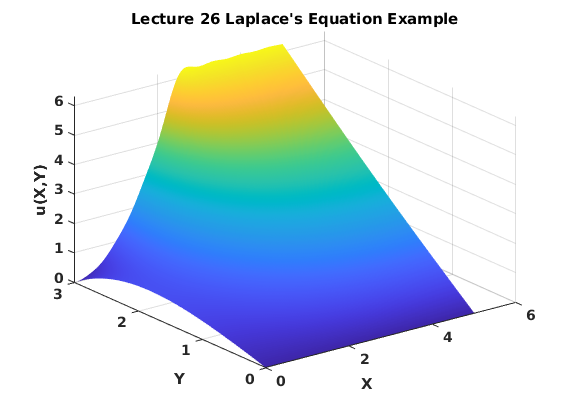
\includegraphics{lec26-ex1-sol.png}
\caption{Surface plot of solution to example problem.}
\label{fig:lec26-ex1-sol}
\end{marginfigure}

\section{Superposition Principle}

In the last example problem, all of the boundary conditions were homogeneous except for along the top edge of the rectangular domain at $y=b$.  We were able to use separation of variables and find a solution because there was one spatial dimension along which \emph{both boundaries were homogeneous.}  Specifically, the boundaries at $x=0$ and $x=a$ had homogeneous type 2 boundary conditions.\marginnote[-1.5cm]{In all of the boundary value problems we have solved so far, this condition has always been met.  In the heat equation and wave equation boundary value problems, there were always homogeneous boundary conditions in the separated boundary value problem for the spatial independent variable $(x)$.  The separated boundary value problem for the temporal independent variable $(t)$ had non-homogeneous boundary (initial) conditions.}   

\begin{marginfigure}
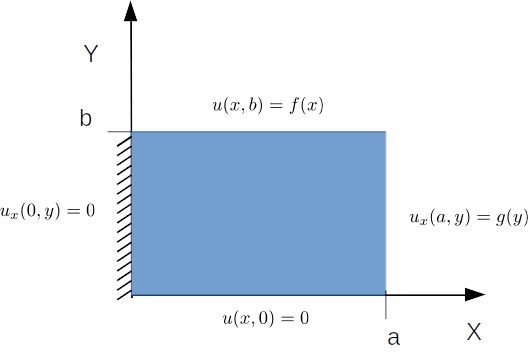
\includegraphics{lec26-ex2-bcs.png}
\caption{Neither spatial dimension has all homogeneous boundary conditions.}
\label{fig:lec26-ex2-bcs}
\end{marginfigure}
What if, instead, we had boundary conditions as depicted by Figure \ref{fig:lec26-ex2-bcs}.  If these were boundary conditions for Laplace's equation, we would carry out separation of variables to derive the two separated boundary value problems just as before.
\begin{align*}
F_{xx}+\lambda F &= 0 \\
G_{yy}-\lambda G &= 0
\end{align*}
Suppose we assumed $\lambda = 0$ and tried to find solutions for $F(x)$, we would get:
\begin{align*}
F(x) &= c_1 x + c_2 \\
F(0) &= c_1 (0) +  c_2 = 0 \\
\Rightarrow c_2 &= 0 \\
F(a) &= c_1(a) = g(y) \ \ \leftarrow \text{  Problem!!}
\end{align*}
Everything is going fine until we have the condition $c_1(a) = g(y)$.  Unless $g(y)$ is a constant: a) no value of $c_1$ will satisfy $g(y)$ for all values of $y \in [0,b]$; and b) there is nothing we can do about it.  We are simply stuck.  The same problem would occur if $\lambda$ were non-zero or if we did the same analysis on $G(y)$.  We need to do something different.


\newthought{What we will do} is this: decompose the problem into two boundary value problems: Problem A and Problem B as is illustrated in Figure \ref{fig:lec26-ex2-bcs-super}.  Each boundary value problem in this decomposition will have one dimension for which there are homogeneous boundary conditions on each boundary.
\begin{marginfigure}
\includegraphics{lec26-ex2-bcs-super.png}
\caption{Superposition of two BVPs each with homogeneous boundary conditions in one dimension.}
\label{fig:lec26-ex2-bcs-super}
\end{marginfigure}
\begin{table}
\begin{tabular}{l l | l}
 & Problem A & Problem B \\ 
 $\substack{\text{Governing} \\ \text{Equation}}$ & $\frac{\partial^2 v}{\partial x^2} + \frac{\partial^2 v}{\partial y^2}=0$ & $\frac{\partial^2 w}{\partial x^2} + \frac{\partial^2 w}{\partial y^2}=0$\\
 & & \\
 $\substack{\text{Boundary}\\\text{Conditions}}$ & $\substack{v_x(0,y) = 0 \ \ v(x,0) = 0\\ v_x(a,y) = 0, \ \ v(x,b)=f(x)}$ & $\substack{w_x(0,y) = 0 \ \ w(x,0) = 0 \\ w_x(a,y) = g(x), \ \ w(x,b) = 0}$
\end{tabular}
\end{table}

\vspace{0.25cm}


\noindent We then solve each boundary value problem to get $v(x,y)$ and $w(x,y)$.  The solution to the original problem is the \emph{superposition} (or just sum) of the solutions to the sub-problems:
\begin{equation*}
u(x,y) = v(x,y) + w(x,y)
\end{equation*}

\vspace{0.25cm}

\noindent\textbf{Notes:}

\begin{enumerate}
\item This superposition method \emph{requires} that the governing equation and boundary conditions for the boundary value problem all be \underline{linear}.  
\item The method also depends on the fact that the governing equation is \underline{homogeneous}.
\item You should break the problem up into as many sub-problems as is required so that, in each sub-problem, there is one dimension (spatial or temporal) that has homogeneous conditions at all boundaries.
\end{enumerate}

\chapter{Lecture 27 - Non-homogeneous Problems}
\label{ch:lec27}
\section{Objectives}
\begin{itemize}
\item Demonstrate a method for solving some non-homogeneous BVPs of the following type:
\begin{enumerate}
\item Non-homogeneous term in the PDE that is a function of no more than one independent variable; and/or
\item constant non-homogeneous term in a boundary condition.
\end{enumerate}
\item Do an example problem.
\end{itemize}
\setcounter{lstannotation}{0} %hack to try and re-set annotation counter.

\section{Time-Independent PDEs and BCs}
Consider the following BVP based on the heat equation:
\begin{table}
\begin{tabular}{l l}
$\substack{\text{Governing} \\\text{Equation}}: $& $\frac{\partial u}{\partial t} = \alpha^2 \frac{\partial^2 u}{\partial x^2} + S(x), \ \ \alpha>0, \ \ 0<x<L, \ \ t>0$ \\
& \\
$\substack{\text{Boundary} \\ \text{Conditions}}: $& $u(0,t)=u_0, \ \ u(L,t) = u_1, \ \ t>0$\\
& \\
$\substack{\text{Initial} \\ \text{Conditions}}: $ & $u(x,0) = f(x), \ \ 0<x<L $ \\
\end{tabular}
\end{table}

\vspace{0.1cm}

\noindent where $u_0$ and $u_1$ are constants.  In this boundary value problem both the governing equation and the boundary conditions are non-homogeneous.  

Since the governing equation is non-homogeneous, it is not separable.  In order to see why, let us begin the separation process:\marginnote[1.5cm]{Here we carry out the steps of separation of variables just as we did in Lecture 23.}
\begin{align*}
u(x,t) &= F(x)G(t) \\
\alpha^2 \frac{\partial^2}{\partial x^2}\left[F(x)G(t)\right] + S(x) &= \frac{\partial}{\partial t}\left[F(x)G(t)\right] \\
\alpha^2 F_{xx}G + S &= FG_t \\
\frac{\alpha^2 F_{xx}G}{\alpha^2 FG} + \frac{S}{\alpha^2 FG} &= \frac{FG_t}{\alpha^2 FG} \\
\frac{F_{xx}}{F} + \underbrace{\frac{S}{\alpha^2 FG}}_{\text{Problem!}} &= \frac{G_t}{\alpha^2 G}
\end{align*}
The term $\sfrac{S}{\alpha^2 FG}$ is a function of both $x$ and $t$ and cannot be separated.

The non-homogeneous boundary conditions are also a problem.  Suppose we were able to complete the separation process and derive separated boundary value problems for $F(x)$ and $G(t)$.  We then try to apply the spatial boundary conditions to $F(x)$:
\begin{align*}
u(0,t) &= F(0)G(t) = u_0 \\
u(L,t) &= F(L)G(t) = u_1
\end{align*}
If we had homogeneous boundary conditions and $u_0=0$---like we have always had before---we could just require $F(0)=0$ and be done with it.\sidenote{Zero is special because if $F(0)=0$, it does not matter what $G(t)$ is, we still satisfy the condition.}  But if $u_1 \ne 0$ we are stuck.  We cannot simply say: $F(0) = \sfrac{u_0}{G(t)}$; even if we knew what $G(t)$ was it could only work in the case that $\sfrac{u_0}{G(t)}$ were a constant.  The same problem applies to the boundary at $x=L$.  If we are to use separation of variables, we need to find a way to make both the governing equation and the boundary conditions homogeneous.

\vspace{0.25cm}

\noindent\textbf{Approach:}
\begin{enumerate}
\item Assume a solution of the form: $u(x,t) = v(x,t) + \psi(x)$.  Inserting this solution into our governing equation gives us:
\begin{align*}
\frac{\partial}{\partial t}\left[v(x,t)+\psi(x)\right]  &= \alpha^2 \frac{\partial^2}{\partial x^2}\left[v(x,t)+\psi(x)\right] + S(x) \\
v_{t} + \cancelto{0}{\psi_{t}}  &= \alpha^2 v_{xx} + \alpha^2 \psi_{xx} + S(x) 
\end{align*}

The boundary conditions become:
\begin{align*}
u(0,t) &= v(0,t) + \psi(0) = u_0 \\
u(L,t) &= v(L,t) + \psi(L) = u_1
\end{align*}
and the initial condition becomes:
\begin{equation*}
u(x,0) = v(x,0) + \psi(x) = f(x)
\end{equation*}

\item Decompose the original boundary value problem into a new, homogeneous boundary value problem for $v(x,t)$ and non-homogeneous boundary value problem for $\psi(x)$:
\begin{table}[h!]
\begin{tabular}{l l}
$\substack{\text{Governing} \\\text{Equation}}: $& $\frac{\partial v}{\partial t} = \alpha^2 \frac{\partial^2 v}{\partial x^2}, \ \ \alpha>0, \ \ 0<x<L, \ \ t>0$ \\
& \\
$\substack{\text{Boundary} \\ \text{Conditions}}: $& $v(0,t)=0, \ \ v(L,t) = 0, \ \ t>0$\\
& \\
$\substack{\text{Initial} \\ \text{Conditions}}: $ & $v(x,0) = f(x)-\psi(x), \ \ 0<x<L $ \\
\end{tabular}
\end{table}

\begin{align*}
\alpha^2 \psi_{xx} + S(x) &= 0 \\
\psi(0) = u_0, \ \ \psi(L) &= u_1
\end{align*}\marginnote[-2.0cm]{Readers are strongly encouraged to look at the boundary value problems for $v(x,t)$ and $\psi(x)$ and see that if you ``add them up'' you recover the original boundary value problem for $u(x,t)$.}
where the non-homogeneous terms from the governing equation and boundary conditions have been absorbed in the equation for $\psi(x)$.  The initial condition for $v(x,t)$ remains non-homogeneous but is modified to account for $\psi(x)$.
\end{enumerate}
We solve for $\psi(x)$, then solve for $v(x,t)$ and add the results together to get $u(x,t)$.

\vspace{0.25cm}

\noindent\textbf{Example:}  Consider the following boundary value problem:
\begin{table}
\begin{tabular}{l l}
$\substack{\text{Governing} \\\text{Equation}}: $& $\frac{\partial u}{\partial t} = \alpha^2 \frac{\partial^2 u}{\partial x^2} + S, \ \ \alpha>0, \ \ 0<x<L, \ \ t>0$ \\
& \\
$\substack{\text{Boundary} \\ \text{Conditions}}: $& $u(0,t)=0, \ \ u(L,t) = u_1, \ \ t>0$\\
& \\
$\substack{\text{Initial} \\ \text{Conditions}}: $ & $u(x,0) = f(x), \ \ 0<x<L $ \\
\end{tabular}
\end{table}

\noindent where $S$ and $u_1$ are constants, as are $\alpha^2$ and $L$; and $f(x)$ is a given function.

\vspace{0.25cm}

\noindent\textbf{Step \#1:} Substitute $u(x,t) = v(x,t) + \psi(x)$.
\begin{table}[h!]
\begin{tabular}{l l}
$\substack{\text{Governing} \\\text{Equation}}: $& $\frac{\partial v}{\partial t} = \alpha^2 \frac{\partial^2 v}{\partial x^2}, \ \ \alpha>0, \ \ 0<x<L, \ \ t>0$ \\
& \\
$\substack{\text{Boundary} \\ \text{Conditions}}: $& $v(0,t)=0, \ \ v(L,t) = 0, \ \ t>0$\\
& \\
$\substack{\text{Initial} \\ \text{Conditions}}: $ & $v(x,0) = f(x)-\psi(x), \ \ 0<x<L $ \\
\end{tabular}
\end{table}

\begin{align*}
\alpha^2 \psi_{xx} + r &= 0 \\
\psi(0) = 0, \ \ \psi(L) &= u_1
\end{align*}

\vspace{0.25cm}

\noindent\textbf{Step \#2:}  Solve for $\psi(x)$.
\begin{align*}
\alpha^2\psi_{xx}+r &= 0 \\
\psi_{xx}(x) &= -\frac{r}{\alpha^2} \\
\psi_{x}(x) &= -\frac{r}{\alpha^2}x + c_1 \\
\psi(x) &= -\frac{r}{2\alpha^2}x^2+c_1x + c_2
\end{align*}
apply boundary conditions
\begin{align*}
\psi(0) &= c_2 = 0 \\
\Rightarrow c_2 &= 0 \\
\psi(L) &= -\frac{r}{2\alpha^2}L^2 + c_1 L = u_1 \\
\Rightarrow c_1 &= \frac{1}{L}\left(u_1+\frac{rL^2}{2 \alpha^2}\right) \\
\Rightarrow \psi(x) &= -\frac{r}{2\alpha^2}x^2 + \frac{1}{L}\left(u_1+\frac{rL^2}{2 \alpha^2}\right)x
\end{align*}

\vspace{0.25cm}

\noindent\textbf{Step \#3:} Solve for $v(x,t)$.

\vspace{0.25cm}

\noindent We have already solved this problem in Lecture 23 and we will not repeat the details here.  The solution is:
\begin{align*}
v(x,t) &= \sum\limits_{n=1}^{\infty} c_n \sin{\frac{n \pi x}{L}}e^{-\left(\alpha \frac{n \pi}{L}\right)^2 t} \\
c_n &= \frac{2}{L} \int_0^L \left[f(x)-\psi(x)\right]\sin{\frac{n \pi x}{L}} \ dx
\end{align*}

\vspace{0.25cm}

\noindent\textbf{Step \#4:} Construct $u(x,t)$ from solutions for $v(x,t)$ and $\psi(x)$.

\begin{align*}
u(x,t) &= \psi(x) + v(x,t) \\
u(x,t) &= -\frac{r}{2\alpha^2}x^2 + \frac{1}{L}\left(u_1+\frac{rL^2}{2 \alpha^2}\right)x + \sum\limits_{n=1}^{\infty} c_n \sin{\frac{n \pi x}{L}}e^{-\left(\alpha \frac{n \pi}{L}\right)^2 t}
\end{align*}
\begin{marginfigure}
\includegraphics{lec27-ex-plt.png}
\caption{The solution, $u(x,t)$ at various times and the steady-state solution $\psi(x)$.}
\label{fig:lec27-ex-plt}
\end{marginfigure}
In this particular case, while we know from the boundary conditions, that $v(x,t)$ goes to zero as $t \rightarrow \infty$, the function $\psi(x)$ remains constant with time.  Conceptually we can think of $\psi(x)$ as being the \emph{steady state} part of the solution while $v(x,t)$ is the \emph{transient} part.

\begin{equation*}
u(x,t) = \underbrace{-\frac{r}{2\alpha^2}x^2 + \frac{1}{L}\left(u_1+\frac{rL^2}{2 \alpha^2}\right)x}_{\text{steady state}} + \underbrace{\sum\limits_{n=1}^{\infty} c_n \sin{\frac{n \pi x}{L}}e^{-\left(\alpha \frac{n \pi}{L}\right)^2 t}}_{\text{transient}}
\end{equation*}
A plot for the case: $\alpha^2 = 0.5$, $L=1$, $r=150$, $u_1=100$, and $f(x) = 300x(1-x)$ is shown in Figure \ref{fig:lec27-ex-plt}.\marginnote{
Take note of how, since the initial condition, $f(x)$, does not match the boundary condition at $x=1$ there is ``wiggliness'' in the Fourier series representation that ``diffuses away'' almost immediately.  Note also how $u(x,\infty)$ matches $\psi(x)$ as expected.} Think about the physics for a minute: we have a rod that is heated from a uniform source, $r$, which gives the roughly parabolic temperature profile throughout the rod except at the ends; the left-hand side is maintained at 0 degrees and the right-hand side is held steady at 100 degrees. Hopefully the answer you see in the plot matches, more-or-less, your expectations as to what the temperature profile \emph{should} look like. 


\chapter{Lecture 28 - Orthogonal Series Expansion}
\label{ch:lec28}
\section{Objectives}
\begin{itemize}
\item Apply separation of variables and solve boundary value problems that have solutions in the form of orthogonal series expansions (other than Fourier series).
\item Show examples with the heat and wave equation.
\end{itemize}
\setcounter{lstannotation}{0} %hack to try and re-set annotation counter.

For some sets of boundary conditions, the solution to the heat equation is an infinite series that is not a Fourier series.  We will show that, apart from details regarding identifying eigenvalues, the implications of this are not large and will have little impact on how you go about computing the solution.  All of this is most easily clarified with a couple of examples.

\vspace{0.3cm}

\noindent\textbf{Example \#1:}  Consider the boundary value problem below based on the heat equation.
\begin{table}
\begin{tabular}{l l}
$\substack{\text{Governing} \\\text{Equation}}: $& $\frac{\partial u}{\partial t} = \alpha^2 \frac{\partial^2 u}{\partial x^2},  \ \ \alpha>0, \ \ 0<x<1, \ \ t>0$ \\
& \\
$\substack{\text{Boundary} \\ \text{Conditions}}: $& $u(0,t)=0, \ \ u_x(1,t) = -hu(1,t), \ \ h>0, \  t>0$\\
& \\
$\substack{\text{Initial} \\ \text{Conditions}}: $ & $u(x,0) = 1, \ \ 0<x<1 $ \\
\end{tabular}
\end{table}
\begin{marginfigure}
\includegraphics{lec28-ex1-schematic.png}
\caption{Schematic of Example \#1.}
\label{fig:lec28-ex1-schematic}
\end{marginfigure}

\vspace{0.1cm}

\noindent A schematic of this problem is shown in Figure \ref{fig:lec28-ex1-schematic}.  On the right end of the domain we have a type 3 boundary condition representing convective heat transfer to an environment maintained at a temperature of 0$^{\circ}$.\marginnote{Note that we have not established any physical units on this system.  If it helps, consider all temperatures given to be in degrees Celsius.}

\vspace{4.0cm}

\newthought{We will solve} this boundary value problem using separation of variables.  Since we have already carried out the separation process for the heat equation numerous times, we will skip ahead and write down the separated equations:
\begin{align*}
u(x,t) &= F(x)G(t) \\
F_{xx} + \lambda F &= 0 \\
G_{t} + \alpha^2 \lambda G &= 0 
\end{align*}
We need to find values of $\lambda$ for which non-trivial solutions to the equations can satisfy the boundary conditions.  Since $F(x)$ is the spatial variable to which the boundary conditions apply, and both boundary conditions are homogeneous, we will focus our attention on the equation for $F(x)$.

\vspace{0.25cm}

\noindent \underline{$\lambda = 0$}:

\begin{align*}
F_{xx} &= 0 \\
F(x) &= c_1x + c_2 \\
F(0) &= c_1(0) + c_2 = 0 \\
\Rightarrow c_2 &= 0 \\
F_x{1} &= c_1 = -hc_1(1) \\
\Rightarrow c_1&= 0
\end{align*}\marginnote[-1.5cm]{Since $h>0$, the only way that $c_1 = -h c_1$ is if $c_1 = 0$.  If $c_1$ were not zero, the last line would imply that $h = -1$ which, since $h>0$, is a contradiction.} So we will rule out $\lambda=0$ since only the trivial solution $F(x)=0$ applies.

\vspace{0.25cm}

\noindent \underline{$\lambda < 0$}:  $\ \ \lambda = -\nu^2, \ \nu>0$.

\begin{align*}
&F_{xx} - \nu^2F = 0 \\
&F(x) = c_1 \cosh{\nu x} + c_2 \sinh{\nu x} \\
&F(0) = c_1(1) + c_2(0) = 0 \\
&\Rightarrow c_1 = 0 \\
&F_{x}(1) = \nu c_2 \cosh{\nu} = -h c_2 \sinh{\nu} \\
&\frac{\nu}{h}c_2 = -c_2\tanh{\nu} \\
&\Rightarrow c_2 = 0
\end{align*}
\begin{marginfigure}
\includegraphics{lec28_plot_of_tanh.png}
\caption{Plot of $\tanh{(\nu)}$.}
\label{fig:lec28-plot-of-tanh}
\end{marginfigure}
Since $\nu>0$ and $h>0$, and, as shown by Figure \ref{fig:lec28-plot-of-tanh} $\tanh{\nu}$ is also positive, $c_2$ must also be equal to zero.\sidenote{By this time, the reader should be getting pretty good at making these kinds of observations.}

\vspace{5.0cm}

\noindent \underline{$\lambda > 0$}: $\ \ \lambda = \nu^2, \ \nu>0$.

\begin{align*}
&F_{xx} + \nu^2 F = 0  \\
&F(x) = c_1 \cos{\nu x} + c_2 \sin{\nu x} \\
&F(0) = c_1 (1) + c_2 (0) = 0 \\
&\Rightarrow c_1 = 0 \\
&F_{x}(1) = \nu c_2 \cos{\nu} = -h c_2 \sin{\nu} \\
&c_2 \tan{\nu} = -\frac{\nu}{h}
\end{align*}
\begin{marginfigure}
\includegraphics{lec28-fig2.png}
\caption{Plot of $\tan{\nu}$ and $-\sfrac{\nu}{h}$ vs $\nu$ for $h=1$.}
\label{fig:lec28-fig2}
\end{marginfigure}
Of course $c_2 = 0$ would satisfy this condition but we are looking for non-trivial solutions.  We see from Figure \ref{fig:lec28-fig2} that the plot of $\tan{\nu}$ intersects the plot of $-\sfrac{\nu}{h}$ infinitely many times.\sidenote{This is the sort of claim for which a mathematician might reasonably expect a proof but, as engineers, we will simply not provide one.  We know $\tan{\nu}$ is periodic and the pattern will continue indefinitely and the straight line $-\sfrac{\nu}{h}$ will intersect each period no matter the value of $h$ and that will be good enough for us.}  The values of $\nu$ where this happens will be used to find our eigenvalues, $\nu_n^2$, and the eigenfunctions will be $F_n(x) = c_n \sin{\nu_n x}$.  Applying these eigenvalues to our separated equation $G(t)$ gives us:

\begin{align*}
&G_{t} + \alpha^2 \nu^2 G = 0 \\
&G_n(t) = c_3e^{-\left(\alpha \nu_n \right)^2 t}
\end{align*}
and the product solution is:
\begin{equation*}
u(x,t) = \sum\limits_{n=1}^{\infty} c_n \sin{(\nu_n x)}e^{-\left(\alpha \nu_n \right)^2t}
\end{equation*}

\vspace{0.25cm}

\noindent Now we must apply the initial condition:
\begin{equation*}
u(x,0) = \sum\limits_{n=1}^{\infty}c_n \sin{(\nu_n x)}\cancelto{1}{e^{0}} = f(x)
\end{equation*}
On the left side of the equation above we have an infinite series with unknown coefficients $c_n$; on the right side we have a given function $f(x)$.  Our job is to find the values $c_n$ so that the two sides are, in fact, equal.  To do this we will multiply both sides of the equation by our orthogonal functions---$\sin{(\nu_n x)}$---and integrate over the interval $x \in [0,1]$.\sidenote{We should hasten to add---``and weight function''---to this phrase.  It is an important detail that is easy to forget.  When we move on to problems in polar and cylindrical coordinates we will need to be more strict about this. }   At this point we still have not nailed down the numeric values of $\nu_n$ but we \emph{do} know that, since the separated boundary value problem for $F(x)$ from which we obtained $\nu_n$ and $\sin{(\nu_n x)}$ fall within the realm of Sturm-Liouville eigenvalue theory, the eigenfunctions are mutually orthogonal with respect to the weight function, $p(x)$ which, in this case, can be shown to be $p(x)=1$. 

The coefficients are given by:
\begin{equation*}
c_n = \frac{\left(f(x),\sin{(\nu_n x)}\right)}{\left( \sin{(\nu_n x)}, \sin{(\nu_n x)}\right)} = \frac{\int_0^1 f(x) \sin{(\nu x)}\ dx}{\int_0^2 \sin{(\nu x)}^2 \ dx}
\end{equation*}

\newthought{We will use} MATLAB to construct our solution to this boundary value problem.  As usual, we will start by clearing out the MATLAB workspace, specify our constants and initial conditions and determine the number of terms to use in our infinite series for $u(x,t)$.

\begin{lstlisting}[name=lec28-ex1, style=myMatlab]
clear
clc
close 'all'

%% Parameters
alpha_sq = 0.1; % thermal diffusivity
h = 10; % convective heat transfer coefficient
L = 1;
f = @(x) 1; % initial condition

N = 25; % number of eigenfunctions


\end{lstlisting}

Next we must find numeric values for $\nu_n$.  To do this, we will observe from Figure \ref{fig:lec28-ex1-schematic} that there is exactly one intersection of $\tan{\nu}$ and $-\sfrac{\nu}{h}$ in the interval $\nu \in [\sfrac{\pi}{2}, \sfrac{3\pi}{2}]$ and another intersection in the interval $\nu \in [\sfrac{3\pi}{2}, \sfrac{5\pi}{2}]$ etcetera.  We keep looking in intervals $[\sfrac{n \pi}{2},\sfrac{(n+2)\pi}{2}], \ \ n=1,3,5,\dots$.  This is done using the MATLAB built-in function \lstinline[style=myMatlab]{fzero()}.
\marginnote[1.0cm]{
\ref{lst:ann28-1-1} \lstinline[style=myMatlab]{fzero()} is a root-finding function so we need to re-formulate $\tan{\nu} = -\sfrac{\nu}{h}$ so a root-finder can get the values of $\nu$.

\vspace{0.25cm}

\ref{lst:ann28-1-2} We do not want to evaluate our function at the ends of the search interval since those correspond to asymptotes of $\tan{x}$.  We move our search boundaries ``in'' a little bit (towards the interior of the interval) to avoid those asymptotes.

}
\begin{lstlisting}[name=lec28-ex1, style=myMatlab]
%% Find the desired number of eigenvalues
ev_fun = @(x) tan(x) + x./h; /*!\annotation{lst:ann28-1-1}!*/

nu = nan(N,1);
delta = 1e-8; /*!\annotation{lst:ann28-1-2}!*/
x0 = [pi/2+delta,3*pi/2-delta];
for i = 1:N
   [x,fval,exit_flag] = fzero(ev_fun,x0); /*!\annotation{lst:ann28-1-3}!*/
   nu(i) = x;
   x0 = x0 + pi;
end
% do some crude error checking
assert(min(diff(nu))>0,...
    'Error! Something is wrong with your eigenvalues!');/*!\annotation{lst:ann28-1-4}!*/

\end{lstlisting}
\noindent \ref{lst:ann28-1-3} In this instance \lstinline[style=myMatlab]{fzero()} has two arguments and returns three values.  The variable \lstinline[style=myMatlab]{ev_fun} is a handle\sidenote{A variable that, when evaluated, returns a function is often referred to as a \emph{handle} to the function.  This is similar to the variable \lstinline[style=myMatlab]{gca} which can be thought of as a handle to the current axis.} to the function to which we are looking for roots and \lstinline[style=myMatlab]{x0} is the interval where we are searching for the roots.  Of the return arguments: \lstinline[style=myMatlab]{x} is the root; \lstinline[style=myMatlab]{fval} is the numeric value of \lstinline[style=myMatlab]{ev_fun} evaluated at the root \lstinline[style=myMatlab]{x}; and \lstinline[style=myMatlab]{exit_flag} is a value returned by \lstinline[style=myMatlab]{fzero()} to indicate if the function was successful or not.\sidenote{See the documentation for a description of the possible values for \lstinline[style=myMatlab]{exit_flag}.  Several built-in MATLAB functions use this output variable and a value of \lstinline[style=myMatlab]{exit_flag=1} normally indicates success.  As you can see, we do not check the value of \lstinline[style=myMatlab]{exit_flag} in this script (and we also ignore \lstinline[style=myMatlab]{fval}) but readers are encouraged to make use of this kind of feedback from MATLAB functions when the reliability of their results is important.}

\vspace{0.25cm}

\noindent \ref{lst:ann28-1-4} This is a modest bit of error checking to ensure that, at a minimum, the roots we find are distinct.

\vspace{0.25cm}

\noindent The remainder of the MATLAB script is typical of what we have been doing so far.

\begin{lstlisting}[name=lec28-ex1, style=myMatlab]
%% Construct solution
Fn = @(x,n) sin(nu(n).*x);
Gn = @(t,n) exp(-(nu(n).^2).*alpha_sq.*t); 

u = @(x,t) 0;

for n = 1:N
   ef_mag = integral(@(x) Fn(x,n).*Fn(x,n),0,L); /*!\annotation{lst:ann28-1-5}!*/
   cn = integral(@(x) f(x).*Fn(x,n),0,L)./ef_mag;
   
   u = @(x,t) u(x,t) + cn*Fn(x,n).*Gn(t,n);
end

\end{lstlisting}
\marginnote[-2.0cm]{
\ref{lst:ann28-1-5}  We have not bothered to try and derive a closed-form solution for $\int_0^1 \sin{\left(\nu_n x \right)} \ dx$ so we do it numerically.
}
\begin{marginfigure}
\includegraphics{lec28-ex1-sol.png}
\caption{Solution for Example \#1.}
\label{fig:lec28-ex1-sol}
\end{marginfigure}
The solution for the parameters we have selected, plotted at various times, is shown in Figure \ref{fig:lec28-ex1-sol}.

Some questions that you should make sure that you can answer:%\marginnote{
%Rough answers:
%\begin{enumerate}
%\item The steady-state temperature is $u(x,\infty)=0$.  Heat passes out the left and right boundary by conduction on the left and convection on the right.

%\item This is because the initial condition $f(x)=1$ did not satisfy the boundary condition at $x=0$.  As expected, the ``wiggliness'' quickly diffuses away.

%\item If the thermal diffusivity is increased, the temperature progresses towards its steady-state value more quickly.

%\item If the convective heat transfer coefficient is increased, energy is transferred through the right boundary more quickly.  This can most easily be observed by noting the \emph{slope} of the solution at the boundary.  If $h$ is increased, the slope becomes more negative; if $h$ is decreased, the slope becomes less negative.  The limit of $h=0$ corresponds to $u_x(1,t)=0$ which is insulated boundary conditions.


%\end{enumerate}
%}
\begin{enumerate}
\item What is the final steady-state temperature?  Answer: zero since all of the energy from the initial condition is transferred out via the left or right boundaries.

\item Why is the initial condition so ``wiggly''? Answer: because the initial condition does not match the boundary condition at $x=0$ and the discontinuity causes perturbations typical of Fourier series.

\item What happens if $\alpha^2$ is increased or decreased?

\item What happens if $h$ is increased or decreased?
  
\end{enumerate}
\begin{figure}[h!]
\subfloat[]{\includegraphics[width=1.8in]{lec28-ex1-sol-alpha-high.png}}
\subfloat[]{\includegraphics[width=1.8in]{lec28-ex1-sol-alpha-low.png}} \\
\subfloat[]{\includegraphics[width=1.8in]{lec28-ex1-sol-h-high.png}}
\subfloat[]{\includegraphics[width=1.8in]{lec28-ex1-sol-h-low.png}}
\label{fig:lec28-ex1-variations}
\caption{Variations in $\alpha$ and $h$ for example problem.}
\end{figure}
Answers to the last two questions are illustrated in Figure \ref{fig:lec28-ex1-variations}.  Images a) and b) illustrate how the solution changes when thermal diffusivity is increased or decreased, respectively.  Images c) and d) illustrate how the solution changes when the convective heat transfer coefficient, $h$, is increased and decreased.

\vspace{0.5cm}

\noindent\textbf{Example \#2:} The twist angle $\theta(x,t)$ of a torsionally vibrating shaft is given by the wave equation.

\begin{table}[h]
\begin{tabular}{l l}
$\substack{\text{Governing} \\\text{Equation}}: $& $\alpha^2 \frac{\partial^2 \theta}{\partial x^2} =  \frac{\partial^2 \theta}{\partial t^2},  \ \ \alpha>0, \ \ 0<x<1, \ \ t>0$ \\
& \\
$\substack{\text{Boundary} \\ \text{Conditions}}: $& $\theta(0,t)=0, \ \ \theta_x(1,t) = 0, \ \ t>0$\\
& \\
$\substack{\text{Initial} \\ \text{Conditions}}: $ & $\theta(x,0) = x, \ \ \theta_t(x,0) = 0, \ \ 0<x<1 $ \\
\end{tabular}
\end{table}
\begin{marginfigure}
\includegraphics{lec28-ex2-schematic.png}
\caption{Schematic of Example \#2.}
\label{fig:lec28-ex2-schematic}
\end{marginfigure}


\newthought{Of course we} will also use separation of variables for this boundary value problem and, again, since we have already carried out the separation process for the wave equation numerous times, we will again skip ahead and write down the separated equations:

\begin{align*}
\theta(x,t) &= F(x)G(t) \\
F_{xx} + \lambda F &= 0 \\
G_{tt} + \alpha^2 \lambda G &= 0
\end{align*}
We need to find values of $\lambda$ for which non-trivial solutions to the equations can satisfy the boundary conditions.  As with the first example, $F(x)$ is the spatial variable to which the boundary conditions apply and both boundary conditions are homogeneous.  Thus we will again focus our attention on the equation for $F(x)$.

\vspace{0.25cm}

\noindent\underline{$\lambda = 0$}:

\begin{align*}
F_{xx} &= 0 \\
F(x) &= c_1x + c_2 \\
F(0) &= c_1(0) + c_2 = 0 \\
\Rightarrow c_2 &= 0 \\
F_{x}(0) &= c_1 = 0 \\
\Rightarrow c_1 &= 0
\end{align*}
We see that for $\lambda = 0$ only the trivial solution can satisfy the boundary conditions.

\vspace{0.25cm}

\noindent\underline{$\lambda < 0$}: $\ \lambda = \nu^2, \ \nu>0$.
\begin{align*}
&F_{xx} - \nu^2 F = 0 \\
&F(x) = c_1 \cosh{\nu x} + c_2 \sinh{\nu x} \\
&F(0) = c_1(1) + c_2(0) = 0 \\
&\Rightarrow c_1 = 0 \\
&F_{x}(1) = \nu c_2 \cosh{\nu} = 0
\end{align*} \marginnote{By this point in time, this analysis may begin to feel quite repetitive.  That is because it \emph{is} repetitive.  Nonetheless, resist the tendency to rush and/or become complacent.  It is worth your while to patiently and carefully work through each of these cases every time.}
For the last conditions, since $\cosh{\nu}$ is always positive for $\nu>0$, $c_2 = 0$ and, again, only the trivial solution can satisfy the boundary conditions.

\vspace{0.25cm}

\noindent\underline{$\lambda > 0$}: $\ \lambda = \nu^2, \ \nu>0$.
\begin{align*}
&F_{xx} + \nu^2 F = 0 \\
&F(x) = c_1\cos{\nu x} + c_2 \sin{\nu x} \\
&F(0) = c_1(1) + c_2(0) = 0 \\
&\Rightarrow c_1 = 0 \\
&F_{x}(1) = \nu c_2 \cos{\nu} = 0
\end{align*}
We can satisfy this boundary condition for any value of $c_2$ provided that $\nu$ is a root of $\cos(x)$.  This happens when $\nu$ is an odd-integer multiple of $\sfrac{\pi}{2}$.  Thus:

\begin{align*}
\nu_n &= (2n-1)\frac{\pi}{2}, \ n=1,2,3\dots \\
F_n(x) &= c_n \sin{\nu_n x}
\end{align*} 
The corresponding solution to $G(t)$ is:
\begin{align*}
&G_{tt} + \alpha^2 \nu_n^2 G = 0 \\
&G(t) = a_n \cos{(\alpha \nu_n t)}+b_n\sin{(\alpha \nu_n t)}
\end{align*}
and the product solution is:
\begin{equation*}
u(x,t) = F(x)G(t) = \sum\limits_{n=1}^{\infty} \left[a_n \cos{(\alpha \nu_n t)}+b_n\sin{(\alpha \nu_n t)} \right]\sin{(\nu_n x)}
\end{equation*}

\newthought{To solve for} the remaining constants $a_n$ and $b_n$ we need to apply the initial conditions.
\begin{align*}
u(x,0) &= \sum\limits_{n=1}^{\infty}\left[a_n(1) + b_n(0) \right]\sin{(\nu_n x)} \\
&=\sum\limits_{n=1}^{\infty} a_n \sin{(\nu_n x)} = x
\end{align*}
To solve for $a_n$, we now only need to multiply both sides by our orthogonal function---$\sin{(\nu_n x)}$---and integrate.  The resulting formula for $a_n$ is:\marginnote[1.0cm]{This really \emph{looks} like a Fourier series, but technically it is not since the expansion functions are not $\sin{(\sfrac{n \pi x}{L})}$ or $\cos{(\sfrac{n \pi x}{L})}$.}
\begin{equation*}
a_n = \frac{(x,\sin{(\nu_n x)})}{(\sin{(\nu_nx)},\sin{(\nu_n,x)})} = \frac{\int_{0}^{1}x \sin{(\nu_n x)} \ dx}{\underbrace{\int_0^1 \sin{(\nu_n x)}^2 \ dx}_{\sfrac{1}{2}}}
\end{equation*}

\vspace{0.25cm}

\noindent The other boundary condition is applied to get $b_n$:
\begin{align*}
u_t(x,0) &= \sum\limits_{n=1}^{\infty} \left[-\alpha \nu_n a_n (0) + \alpha \nu_n b_n(1)\right]\sin{(\nu_n x)} = 0 \\
\Rightarrow b_n &= 0, \ \ n=1,2,3\dots
\end{align*}

\noindent In summary, the solution is:
\begin{align*}
u(x,t) &= \sum\limits_{n=1}^{\infty} a_n \cos{(\alpha \nu_n t)}\sin{(\nu_n x)} \\
a_n &= 2 \int_0^1 x \sin{(\nu_n x)} \ dx
\end{align*}

\newthought{The MATLAB code} to construct and visualize the solution for this problem is shown in the listing below.

\begin{lstlisting}[name=lec28-ex2, style=myMatlab]
clear
clc
close 'all'

%% Parameters
alpha_sq = 5;
L = 1;
N = 30;

nu = @(n) (2*n-1)*pi/2;
Fn = @(x,n) sin(nu(n).*x);
Gn = @(t,n) cos(alpha_sq*nu(n).*t);
f = @(x) x; % initial displacement
u = @(x,t) 0; % initial velocity

for n = 1:N
   ef_mag = integral(@(x) Fn(x,n).^2,0,L);
   an = integral(@(x) f(x).*Fn(x,n),0,L)./ef_mag;   
   u = @(x,t) u(x,t) + an.*Fn(x,n).*Gn(t,n);
end

%% Plot the solution
Nx = 1000;
X = linspace(0,L,Nx);

Tmax = 5;
Nt = 50;
T = linspace(0,Tmax,Nt);

figure(2)
for t = 1:Nt
    plot(X,u(X,T(t)),'-b','linewidth',3);
    title_str = sprintf('Lecture 28 Example 2, t = %g ',T(t));
    title(title_str,'fontsize',16,'fontweight','bold');
    xlabel('X','fontsize',14,'fontweight','bold');
    ylabel('U(X,T) Angular Displacement', 'fontsize',14,...
        'fontweight','bold');
    grid on
    set(gca,'fontsize',12,'fontweight','bold');
    axis([0 L -L L]);
    pause(Tmax/(Nt-1));    
end
\end{lstlisting}


\chapter{Assignment \#10}
\label{ch:ass10}
\begin{fullwidth}

\begin{enumerate}
\item Solve the boundary value problem below using separation of variables.
\begin{table}[h]
\begin{tabular}{l l}
$\substack{\text{Governing} \\\text{Equation}}: $& $\frac{\partial^2 u}{\partial x^2} + \frac{\partial^2 u}{\partial y^2} = 0, \ \ 0<x<a, \ \ 0<y<b $\\
& \\
$\substack{\text{Boundary} \\ \text{Conditions}}: $ & $\substack{u(x,0)=0  \ \ \ \ \ \ u(0,y) = 0 \\ \\ u(x,b) = f(x) \ \ u(a,y) = 0}$ 
\end{tabular}
\end{table} 


\vspace{2.0cm}

\item Solve the boundary value problem below using separation of variables.
\begin{table}[h]
\begin{tabular}{l l}
$\substack{\text{Governing} \\\text{Equation}}: $& $\frac{\partial^2 u}{\partial x^2} + \frac{\partial^2 u}{\partial y^2} = 0, \ \ 0<x<1, \ \ 0<y<1 $\\
& \\
$\substack{\text{Boundary} \\ \text{Conditions}}: $ & $\substack{u_y(x,0)=0  \ \ \ \ \ \ u(0,y) = 0 \\ \\ u_y(x,1) = 0 \ \ u(1,y) = 1-y}$ 
\end{tabular}
\end{table} 

\noindent Symbolically solve the problem and set up, but do not evaluate analytically, the Fourier coefficients.  Use MATLAB to numerically find the solution using $N=15$ eigenmodes.  Plot the solution using the MATLAB built-in function \lstinline[style=myMatlab]{surf()} and print out the value of the solution at $u(0.5,0.5)$.

\vspace{2.0cm}

\item Solve the non-homogeneous boundary value problem below.
\begin{table}
\begin{tabular}{l l}
$\substack{\text{Governing} \\\text{Equation}}: $& $\frac{\partial u}{\partial t} = \alpha^2 \frac{\partial^2 u}{\partial x^2} + Ae^{-\beta x}, \ \ \alpha>0, \ \beta>0, \ \ 0<x<1, \ \ t>0$ \\
& \\
$\substack{\text{Boundary} \\ \text{Conditions}}: $& $u(0,t)=0, \ \ u(1,t) = 0, \ \ t>0$\\
& \\
$\substack{\text{Initial} \\ \text{Conditions}}: $ & $u(x,0) = f(x), \ \ 0<x<L $ \\
\end{tabular}
\end{table}

\vspace{2.0cm}

\item Find a steady-state solution $\psi(x)$ of the non-homogeneous boundary value problem below.

\begin{table}
\begin{tabular}{l l}
$\substack{\text{Governing} \\\text{Equation}}: $& $\frac{\partial u}{\partial t} = \alpha^2 \frac{\partial^2 u}{\partial x^2} -h(u-u_0), \ \ \alpha>0, \ h>0, \ \ 0<x<1, \ \ t>0$ \\
& \\
$\substack{\text{Boundary} \\ \text{Conditions}}: $& $u(0,t)=u_0, \ \ u(1,t) = 0, \ \ t>0$\\
& \\
$\substack{\text{Initial} \\ \text{Conditions}}: $ & $u(x,0) = f(x), \ \ 0<x<L $ \\
\end{tabular}
\end{table}

\vspace{2.0cm}

\item Solve the boundary value problem below using separation of variables.
\begin{table}[h]
\begin{tabular}{l l}
$\substack{\text{Governing} \\\text{Equation}}: $& $\frac{\partial^2 u}{\partial x^2} + \frac{\partial^2 u}{\partial y^2} = 0, \ \ 0<x<1, \ \ 0<y<1 $\\
& \\
$\substack{\text{Boundary} \\ \text{Conditions}}: $ & $\substack{u(x,0)=0  \ \ \  \ \ u_x(0,y) = 0 \\ \\ u_y(x,1) = 0 \ \ \ \ u(1,y) = u_0}$ 
\end{tabular}
\end{table} 

\vspace{0.25cm}

\noindent Solve the equation symbolically.  Use MATLAB to represent the solution for $N=15$ eigenmodes with $u_0=0.25$.  Plot the solution using MATLAB's built-in function \lstinline[style=myMatlab]{surf()}.

\end{enumerate}

\end{fullwidth}



\chapter{Lecture 29 - Fourier Series in Two Variables}
\label{ch:lec29}
\section{Objectives}
\begin{itemize}
\item Present Fourier series expansions in two (or more) independent variables.
\item Show an example application in the solution to the heat equation in two spatial dimensions.
\end{itemize}
\setcounter{lstannotation}{0}

\section{Fourier Series Expansion in Two Variables}

Consider the function $f(x,y), \ 0<x<a, \ 0<y<b$.  Suppose we want to represent the function in the form of a \emph{double} Fourier series as follows:

\begin{equation}
f(x,y) = \sum\limits_{m=1}^{\infty}\sum\limits_{n=1}^{\infty} A_{mn}\sin{\frac{m\pi y}{a}} \sin{\frac{n \pi x}{b}}
\label{eq:double-fourier}
\end{equation}

\begin{enumerate}

\item Should we expect this to be possible?  Answer: of course!  Fourier series have shown themselves to be a perfectly adequate tool for representing a variety of functions.  There is no problem in adding another spatial dimension.

\item How will we determine the appropriate values for $A_{mn}$?  Answer: we will multiply both sides by orthogonal function\underline{s} and integrate, as usual.\marginnote{Again, these sets of functions---$\sin{\sfrac{m \pi x}{a}}$ and $\sin{\sfrac{n \pi y}{b}}$---are orthogonal with respect to a weight function $p(x)=1$ and we should not forget it even if we leave it out of the equations and fail to mention it in the discussion.}

\end{enumerate}
\begin{multline*}
\int_0^b \int_0^a f(x,y) \sin{\frac{m^{\prime} \pi x}{a}} \sin{\frac{n^{\prime} \pi y}{b}} \ dx \ dy = \cdots \\ \int_0^a \int_0^b A_{mn}\sin{\frac{m \pi x}{a}} \sin{\frac{n \pi y}{b}}\sin{\frac{m^{\prime} \pi x}{a}} \sin{\frac{n^{\prime} \pi y}{b}} \ dx \ dy
\end{multline*}
where, if $m^{\prime}=m$ and $n^{\prime} = n$ then:\marginnote{Of course, if $m^{\prime}\ne m$ or $n^{\prime} \ne n$ then the respective integral is zero by orthogonality.}
\begin{multline*}
\int_0^b \int_0^a f(x,y) \sin{\frac{m^{\prime} \pi x}{a}} \sin{\frac{n^{\prime} \pi y}{b}} \ dx \ dy = \cdots \\ A_{mn} \underbrace{\left[\int_0^a \sin{(\frac{m \pi x}{a})}^2 \ dx \right]}_{=\frac{a}{2}} \underbrace{ \left[ \int_0^b \sin{(\frac{n \pi y}{b})}^2 \ dy \right]}_{=\frac{b}{2}}
\end{multline*}
So that
\begin{equation}
A_{mn} = \frac{4}{a b} \int_0^b \int_0^a f(x,y) \sin{\frac{m \pi x}{a}} \sin{\frac{n \pi y}{b}} \ dx \ dy
\label{eq:double-fourier-coeff}
\end{equation}

\section{MATLAB Implementation}
Implementing this expansion in MATLAB is mostly straight-forward.  We will start by defining parameters:
\marginnote{

\vspace{4.0 cm}

\ref{lst:ann29-1-1} Here we use a \lstinline[style=myMatlab]{switch...case} selection structure.  For the in-class demonstration I like to choose between different functions for which the double Fourier expansion will be used.  The parameter \lstinline[style=myMatlab]{ex_select} is set to either 1 or 2; the \lstinline[style=myMatlab]{case} statements allow me to assign a function handle to \lstinline[style=myMatlab]{f} accordingly.  The \lstinline[style=myMatlab]{otherwise} statement allows me to gracefully deal with having specified an invalid value for \lstinline[style=myMatlab]{ex_select}.

}
\begin{lstlisting}[name=lec29-ex1, style=myMatlab]
clear
clc
close 'all'

%% Parameters
a = 4;
b = 3;

N = 20;

ex_select = 1;
% 1 smooth
% 2 not smooth

switch ex_select  /*!\annotation{lst:ann29-1-1}!*/
    case 1
        f = @(x,y) x.*(a-x).*y.*(b-y);
        
    case 2
       f = @(x,y) ex1(x,y,a,b);
       
    otherwise
        error('Invalid Example Choice!');
end
\end{lstlisting}

\noindent Next we will visualize the function that we hope to represent with a double Fourier series.

\begin{lstlisting}[name=lec29-ex1,style=myMatlab]
Nx = 250;
Ny = 250;

X = linspace(0,a,Nx);
Y = linspace(0,b,Ny);

[XX,YY] = meshgrid(X,Y);

figure(1)
surf(XX,YY,f(XX,YY),'edgecolor','none');
title('f(x,y)','fontsize',16,'fontweight','bold');
xlabel('X','fontsize',14,'fontweight','bold');
ylabel('Y','fontsize',14,'fontweight','bold');
zlabel('f(X,Y)','fontsize',14,'fontweight','bold');
set(gca,'fontsize',12,'fontweight','bold');


\end{lstlisting}

\begin{figure}[h!]
\subfloat[]{\includegraphics[width=2in]{lec29-fx1.png}}
\subfloat[]{\includegraphics[width=2in]{lec29-fx1-dfexp.png}} \\
\subfloat[]{\includegraphics[width=2in]{lec29-fx2.png}}
\subfloat[]{\includegraphics[width=2in]{lec29-fx2-dfexp.png}}
\label{fig:lec29-dfexp}
\caption{Plots of example functions and their double Fourier series expansions.}
\end{figure}
\noindent Plots of the two example functions along with their double Fourier series expansions are shown in Figure \ref{fig:lec29-dfexp}. 

\vspace{2.0cm}

\noindent The MATLAB code needed to calculate the Fourier coefficients and plot the resulting expansion are provided below:

\begin{lstlisting}[name=lec29-ex1,style=myMatlab]
%% Double Fourier Expansion
Xn = @(x,n) sin(n.*pi.*x./a);
Yn = @(y,n) sin(n.*pi.*y./b);

A = nan(N,N); /*!\annotation{lst:ann29-1-2}!*/
FF = @(x,y) 0;

for m = 1:N
    for n = 1:N
        A(m,n) = integral2(@(x,y) f(x,y).*Xn(x,m).*Yn(y,n),... /*!\annotation{lst:ann29-1-3}!*/
            0,a,0,b)./...
            integral2(@(x,y) (Xn(x,m).^2).*(Yn(y,n).^2),...
            0,a,0,b); %(same as formula - 4/(a*b) above)
        FF = @(x,y) FF(x,y)+A(m,n).*Xn(x,m).*Yn(y,n);
    end
end

figure(2)
surf(XX,YY,FF(XX,YY),'edgecolor','none');
title('Double Fourier Expansion of f(x,y)','fontsize',16,'fontweight','bold');
xlabel('X','fontsize',14,'fontweight','bold');
ylabel('Y','fontsize',14,'fontweight','bold');
zlabel('FF(X,Y)','fontsize',14,'fontweight','bold');
set(gca,'fontsize',12,'fontweight','bold');
\end{lstlisting}

\marginnote[-12.0cm]{Note the ``wiggliness'' present in the double Fourier expansion in the presence of discontinuities.}  

\marginnote[-8.0cm]{
 

\ref{lst:ann29-1-2} The Fourier coefficients are conveniently stored in a two-dimensional matrix.  

\vspace{0.25cm}

\ref{lst:ann29-1-3} We use a double-nested loop to do the calculations.  Note in this implementation we do not make use of the known value of the magnitude of the eigenfunctions.

}

Lastly we need to define the local function for \lstinline[style=myMatlab]{ex1(x)}.  This example is presented to illustrate that the convergence behavior for a double Fourier series is similar to a regular (single) Fourier series.  This function is piece-wise continuous and is defined as:
\begin{equation*}
f(x) = 
\begin{cases}
-1, & x < \frac{a}{2} \text{ and } y < \frac{b}{2} \\
0, & \text{otherwise}
\end{cases}
\end{equation*}
\marginnote[2.8cm]{
\ref{lst:ann29-1-4} Note the use of an assertion to enforce my expectation that the same number of Fourier modes will be used for the expansion in $x$ as is used in the expansion in $y$.
}
\begin{lstlisting}[style=myMatlab, name=lec29-ex1]
%% Local functions
function z = ex1(x,y,a,b)
[mx,nx] = size(x); % write your function to expect vector inputs
[my,ny] = size(y);
% for this implementation, I will expect x and y to have the same size
assert((mx==my) && (nx == ny),...           /*!\annotation{lst:ann29-1-4}!*/
    'error: x and y must have same size');
z = nan(mx,nx); % construct z to be the same as X and Y

% there are fancier ways to do this, but we will use a very simple
% implementation
for i = 1:mx
    for j = 1:nx
        if (x(i,j) < a/2) && (y(i,j) < b/2)
            z(i,j) = -1;
        else
            z(i,j) = 1;
        end
    end
end
end
\end{lstlisting}

\section{Application to Solving a BVP}
In this section we will carry out an example problem that calls for use of a double Fourier series expansion.  Consider the boundary value problem below based on the heat equation. \marginnote{\textbf{Note:} Think about the physics that this boundary value problem represents.  It is the time-dependent heat equation on a rectangular domain. An initial temperature distribution is specified but all of the boundaries are held at a temperature of 0.  Over time, we expect \emph{all} of the energy to exit the domain via the boundaries so the final steady-state temperature is zero everywhere.}

\begin{table}
\begin{tabular}{l l}
$\substack{\text{Governing} \\\text{Equation}}: $& $\frac{\partial u}{\partial t} = \alpha^2 \left(\frac{\partial^2 u}{\partial x^2} + \frac{\partial^2 u}{\partial y^2}\right),  \ \ \alpha>0, \ \ 0<x<a, \ \ 0<y<b, \ \  t>0$ \\
& \\
$\substack{\text{Boundary} \\ \text{Conditions}}: $ & $\substack{u(x,0,t)=0  \ \ \ \ \ \ u(0,y,t) = 0 \\ \\ u(x,b,t) = 0 \ \ u(a,y,t) = 0} \ \ t>0$ \\
& \\
$\substack{\text{Initial} \\ \text{Conditions}}: $ & $u(x,y,0) = f(x,y), \ \ 0<x<a, \ \ 0<y<b $ 
\end{tabular}
\end{table}

\vspace{0.25cm}

\noindent We will solve this problem using separation of variables.

\vspace{0.25cm}

\noindent\textbf{Step \#1:} Assume a product solution.
\begin{equation*}
u(x,y,t) = F(x)G(y)H(t)
\end{equation*}

\vspace{3.0cm}

\noindent\textbf{Step \#2:} Insert proposed solution into the governing equation.

\begin{align*}
\frac{\partial}{\partial t}\left[F(x)G(y)H(t)\right] &= \alpha^2 \left\{\frac{\partial^2}{\partial x^2}\left[F(x)G(y)H(t)\right] + \frac{\partial^2}{\partial y^2}\left[F(x)G(y)H(t)\right] \right\} \\
FGH_t &= \alpha^2\left(F_{xx}GH + FG_{yy}H\right) \\
\end{align*}

\vspace{0.25cm}

\noindent\textbf{Step \#3a:} Separate variables (partially: $x$ from $y$ and $t$).

\begin{align*}
\frac{FGH_t}{\alpha^2 FGH} &= \frac{\alpha^2 F_{xx}GH}{\alpha^2 FGH} + \frac{\alpha^2 FG_{yy}H}{\alpha^2 FGH} \\
\frac{H_t}{\alpha^2 H} &= \frac{F_{xx}}{F} + \frac{G_{yy}}{G} \\
\underbrace{\frac{F_{xx}}{F}}_{\substack{\text{function of} \\ x}} &= \underbrace{-\frac{G_{yy}}{G} + \frac{H_{t}}{\alpha^2 H}}_{\substack{\text{function of} \\ y,t}} = -\lambda \\
&F_{xx} + \lambda F = 0 \\
&\frac{G_{yy}}{G} = \frac{H_{t}}{\alpha^2 H} + \lambda
\end{align*}
\marginnote[-3.5cm]{In this line, the function of $x$ will, in general, only be equal to a function of $y$ and $t$ if they are both equal to some constant.}
\vspace{0.25cm}

\noindent\textbf{Step \#3b:} Separate remaining variables---$t$ from $y$.

\begin{align*}
\frac{G_{yy}}{G} &= \frac{H_{t}}{\alpha^2 H} + \lambda = -\mu \\
G_{yy} + \mu G &= 0 \\
H_{t} + \alpha^2\gamma H &= 0, \text{ where: } \gamma = \lambda + \mu
\end{align*}

\noindent\textbf{Step \#4:} Apply boundary conditions to determine non-trivial product solution(s).
We have solved problems with these boundary conditions many times so, in the interest of brevity, we will simply state the following:\marginnote{Please do not let me tempt you off the virtuous path of analyzing these conditions carefully. You will find the analysis to be similar to what you have done before.}
\begin{align*}
\lambda > 0, \ \ \lambda &= \beta_{m}^2, \ \ \beta_m = \frac{m \pi}{a} \\
\mu>0, \ \ \mu &= \beta_n^2, \ \ \beta_n = \frac{n \pi}{b} \\
F_m(x) &= \sin{\frac{m \pi x}{a}} \\
G_n(y) &= \sin{\frac{n \pi y}{b}} \\
H_{mn}(t) &= e^{-\alpha^2\left[\left(\frac{m \pi}{a}\right)^2 + \left(\frac{n \pi}{b} \right)^2 \right]t} 
\end{align*}
\vspace{0.25cm}

\noindent The product solution is given in Equation \ref{eq:lec29-ex2-sol}.
\begin{equation}
u(x,y,t) = \sum\limits_{m=1}^{\infty} \sum\limits_{n=1}^{\infty} A_{mn} \sin{\left(\frac{m \pi x}{a}\right)} \sin{\left(\frac{n \pi y}{b}\right)}e^{-\alpha^2\left[\left(\frac{m \pi}{a}\right)^2 + \left(\frac{n \pi}{b} \right)^2 \right]t}
\label{eq:lec29-ex2-sol}
\end{equation}

\vspace{0.25cm}

\noindent\textbf{Step \#5:} Satisfy the initial condition.

\begin{align*}
u(x,y,0) &= \sum\limits_{m=1}^{\infty} \sum\limits_{n=1}^{\infty} A_{mn} \sin{\left(\frac{m \pi x}{a}\right)} \sin{\left(\frac{n \pi y}{b}\right)} \cancelto{1}{e^{0}} = f(x,y) \\
&=\sum\limits_{m=1}^{\infty} \sum\limits_{n=1}^{\infty} A_{mn} \sin{\left(\frac{m \pi x}{a}\right)} \sin{\left(\frac{n \pi y}{b}\right)} = f(x,y)
\end{align*}
This is the double Fourier series that we started the lecture with.  The coefficients are given by Equation \ref{eq:lec29-ex2-sol-coeff}.

\begin{equation}
A_{mn} = \frac{4}{a b} \int_0^b \int_0^a f(x,y) \sin{\frac{m \pi x}{a}} \sin{\frac{n \pi y}{b}} \ dx \ dy
\label{eq:lec29-ex2-sol-coeff}
\end{equation}



\part{Boundary Value Problems in Polar, Cylindrical and Spherical Coordinates}
\chapter{Lecture 30 - Laplacian in Polar Coordinates}
\label{ch:lec30}
\section{Objectives}
\begin{itemize}
\item Discuss the derivation of the Laplacian operator in polar coordinates.
\item Do an example in which we solve Laplace's equation (steady-state heat equation) in polar coordinates.
\end{itemize}
\setcounter{lstannotation}{0}

\section{Laplacian Operator in Polar Coordinates}

In past lectures we have used the Laplacian operator ($\nabla^2$ or $\bigtriangleup$) which is shown for rectangular coordinates below.
\begin{align*}
\nabla &= \langle \frac{\partial}{\partial x}, \frac{\partial}{\partial y}, \frac{\partial}{\partial z} \rangle \\
\nabla \cdot \nabla = \nabla^2 &= \frac{\partial^2}{\partial x^2} + \frac{\partial^2}{\partial y^2} + \frac{\partial^2}{\partial z^2} \\
&= \bigtriangleup
\end{align*}
The operator notation is convenient insofar as it is agnostic regarding coordinate system.  We can use the Laplacian in a differential equation---e.g.$\nabla^2u = 0$---without immediate regard as to whether the domain will be described in a rectangular (Cartesian) coordinate system, polar, cylindrical or spherical coordinates.  Still, at some point in time before we can hope to solve such a differential equation, we need to select a coordinate system.\marginnote[-1.5cm]{How do you pick a coordinate system?  The answer is that you select a coordinate system that makes \underline{\emph{the boundary of the domain easy to describe.}}}  Once we have done that, we need to have an expression of the Laplacian available with the appropriate independent variables.  
\begin{marginfigure}
\includegraphics{lec30-cylindrical-coordinates.png}
\caption{Cylindrical coordinate system.}
\label{fig:lec30-cylindrical-coordinates}
\end{marginfigure}

\newthought{We will start} with polar coordinates.  The standard schematic of the cylindrical coordinate system is shown in Figure \ref{fig:lec30-cylindrical-coordinates}; polar coordinates are just cylindrical coordinates without the $z$-dimension.  To derive an expression for the Laplacian operator in polar coordinates, we need to be able to express the independent variables for polar coordinates---$r$ and $\theta$---in terms of the independent variables for rectangular coordinates---$x$ and $y$.  The relations between the respective coordinates are given in the margin.
\begin{margintable}
\begin{tabular}{l l l}
$r^2 = x^2 + y^2$ & & $x = r \cos{\theta} $ \\
 & \multicolumn{1}{c}{or} & \\
 $\theta = \tan^{-1}{(\sfrac{y}{x})}$ & & $y = r \sin{\theta}$\\
 \end{tabular}
\end{margintable}
So to express the Laplacian in polar coordinates, we need to express:
\begin{equation*}
u_{xx} + u_{yy} = 0
\end{equation*}
in terms of $r$ and $\theta$.  We have done changes of variables like this before; we will follow the same process.

Starting with the first derivatives, using the chain rule and product rule we have:
\begin{equation*}
\frac{\partial u}{\partial x} = \frac{\partial u}{\partial r}\frac{\partial r}{\partial x} + \frac{\partial u}{\partial \theta} \frac{\partial \theta}{\partial x}
\end{equation*}
or, using subscript notation:
\begin{equation*}
u_x = u_r r_x + u_{\theta} \theta_x
\end{equation*}
We need to replace every occurrence of $x$ with its equivalent in terms of $r$ and $\theta$. \marginnote[1.5cm]{
\noindent Here we use: 

\vspace{0.1cm}

\noindent $x = r\cos{\theta}$

\vspace{0.1cm}

\noindent and 

\vspace{0.1cm}

\noindent $(x^2 + y^2)^{-\sfrac{1}{2}} = \sfrac{1}{r}$
}
\begin{align*}
r &= \left(x^2 + y^2\right)^{\sfrac{1}{2}} \\
r_x &= 2x \frac{\left(x^2 +y^2\right)^{-\sfrac{1}{2}}}{2} \\
&= \frac{2(r \cos{\theta})}{2r} \\
&= \cos{\theta}
\end{align*}
\marginnote[1.0cm]{
Here we use the product rule and the not-so-familiar fact that:

\vspace{0.1cm}

\noindent $\frac{d}{dx}\tan^{-1}(u) = \frac{1}{1+u^2}$

\vspace{0.8cm}

\noindent $y = r\sin{\theta}$

\vspace{0.25cm}

\noindent $x^2+y^2 = r^2$

}
\begin{align*}
\theta &= \tan^{-1}(\sfrac{y}{x}) \\
\theta_x &= -\frac{y}{x^2}\left(\frac{1}{1+\sfrac{y^2}{x^2}}\right) \\
&= -\frac{y}{x^2 + y^2} \\
&= \frac{-r \sin{\theta}}{r^2} \\
&= -\frac{sin{\theta}}{r}
\end{align*}
So:
\begin{align*}
u_x &= u_r r_x + u_{\theta} \theta_x \\
u_x &= u_r \cos{\theta} - u_{\theta}\frac{\sin{\theta}}{r}
\end{align*}
Repeating the process to find the equivalent of $u_{xx}$:
\begin{align*}
u_{xx} &= \left(u_{x}\right)_{x} \\
&= \left(u_x\right)_r r_x + \left(u_x\right)_{\theta} \theta_x \\
&= \left(u_r \cos{\theta} - u_{\theta}\frac{\sin{\theta}}{r} \right)_r \cos{\theta} - \left( u_r \cos{\theta} - u_{\theta}\frac{\sin{\theta}}{r}\right)_{\theta}\frac{\sin{\theta}}{r}
\end{align*}
We would then start all over again to find $u_y$ and $u_{yy}$.  Balancing mathematical tedium with conceptual understanding, we will omit these details.  Readers are encouraged to finish the job.\sidenote{Like some other hazing rituals, deriving the Laplacian operator for polar coordinates has some (small) redeeming benefits.}

\newthought{After much tedious} work and simplification you can arrive at the expression of the Laplacian in polar coordinates given in Equation \ref{eq:laplacian-polar}.
\begin{equation}
\nabla^2u = \frac{\partial^2 u}{\partial r^2} + \frac{1}{r}\frac{\partial u}{\partial r} + \frac{1}{r^2}\frac{\partial^2 u}{\partial \theta^2}
\label{eq:laplacian-polar}
\end{equation}

We are now ready to solve Laplace's equation in polar coordinates.

\vspace{0.25cm}

\noindent\textbf{Example:} Solve the boundary value problem below based on the steady-state heat equation on a circular plate of radius $c$.

\begin{table}[h]
\begin{tabular}{l l}
$\substack{\text{Governing} \\\text{Equation}}: $& $\frac{\partial^2 u}{\partial r^2} + \frac{1}{r}\frac{\partial u}{\partial r} + \frac{1}{r^2}\frac{\partial^2 u}{\partial \theta^2}= 0, \ \ 0<r<c, \ \ 0<\theta<2 \pi $\\
& \\
$\substack{\text{Boundary} \\ \text{Conditions}}: $ & $u(c,\theta) = f(\theta), \ \ 0 < \theta< 2 \pi$\\
\end{tabular}
\end{table} 
You can confirm that the equation is linear and homogeneous.  As usual, we will use separation of variables to solve the problem.

\vspace{0.25cm}

\noindent\textbf{Step \#1:} Assume a product solution.
\begin{equation*}
u = F(r)G(\theta) 
\end{equation*}

\vspace{0.25cm}

\noindent\textbf{Step \#2:} Insert the product solution into the governing equation.  
\begin{align*}
\frac{\partial^2}{\partial r^2}(FG) + \frac{1}{r}\frac{\partial}{\partial r}(FG) + \frac{1}{r^2}\frac{\partial^2}{\partial \theta^2}(FG) &=0 \\
F_{rr}G + \frac{1}{r}F_rG + \frac{1}{r^2}FG_{\theta \theta} &= 0
\end{align*}

\vspace{0.25cm}

\noindent\textbf{Step \#3:} Separate variables.
\marginnote[2.20cm]{Note the need to multiply through by $r^2$ in order to separate terms that are a function of $r$ from those that are a function of $\theta$.}
\begin{align*}
\frac{F_{rr}G}{FG} + \frac{1}{r}\frac{F_rG}{FG} + \frac{1}{r^2}\frac{FG_{\theta \theta}}{FG} &= 0 \\
\frac{F_{rr}}{F} + \frac{1}{r}\frac{F_r}{F} + \frac{1}{r^2}\frac{G_{\theta \theta}}{G} &= 0 \\
\underbrace{\frac{r^2 F_{rr} + r F_r}{F}}_{\text{function of } r} = \underbrace{-\frac{G_{\theta \theta}}{G}}_{\substack{\text{function of} \\ \theta}} &= \lambda \\
r^2 F_{rr} + r F_{r} - \lambda F &= 0 \\
G_{\theta \theta} + \lambda G &= 0
\end{align*}

\vspace{4.0cm}

\noindent\textbf{Step \#4:} Apply boundary conditions to determine non-trivial product solution(s).  There is only one boundary condition explicitly given in this problem and it applies to the spatial variable $r$.  In this problem, however, there are some important implicit boundary conditions:
\begin{enumerate}
\item The solution must be periodic in $\theta$. This will be needed so that all the eigenfunctions in $\theta$ can be used; and
\item The solution must be finite everywhere.  In particular, it will be important that $\lim_{r\to 0} F(r) < \infty$.  
\end{enumerate}

\vspace{0.15cm}

\noindent\underline{$\lambda = 0$}
We will start with $G(\theta)$:
\begin{align*}
G_{\theta \theta} &= 0 \\
G(\theta) &= c_1 + c_2\theta
\end{align*}
Since the solution must be periodic, with period $2\pi$, $c_2 = 0$.  Consequently $G(\theta) = c_1$ is a non-trivial eigenfunction.

Checking solutions for $F(r)$:
\marginnote{ This is a Cauchy-Euler equation.  Recall from the beginning of the course that we seek solutions of the form $r^{m}$.  Inserting $r^m$ into the equation gives us: $r^2[m(m-1)r^{m-2} + mr^m]=0$ which can be simplified to: $r^m[m(m-1)+m]=0$ which is only true if $m^2 = 0$.  Recall how to deal with this double-root.}
\begin{align*}
r^2F_{rr} + rF_{r} &= 0 \\
F(r) &= c_3 + c_4 \ln{r}
\end{align*}
In order to satisfy our other implicit boundary condition, $c_4 = 0$.  So $F(r)=  c_3$ is also a valid eigenfunction.  Looking ahead, our product solution will include a constant term for the eigenvalue $\lambda = 0$.

\vspace{0.15cm}

\noindent\underline{$\lambda < 0$}: where we set $\lambda = -\nu^2, \ \nu>0$.

For $G(\theta)$:
\begin{align*}
G_{\theta \theta} - \nu^2 G &= 0 \\
G(\theta) &= c_1 \cosh{\nu \theta} + c_2 \sinh{\nu \theta}
\end{align*}
Neither $\cosh{()}$ nor $\sinh{()}$ are periodic so we must conclude that $c_1 = c_2 = 0$ and that there are no non-trivial eigenfunctions for $\lambda < 0$.


\vspace{0.15cm}

\noindent\underline{$\lambda > 0$}: where we set $\lambda = \nu^2, \ \nu>0$.

For $G(\theta)$:
\begin{align*}
G_{\theta \theta} + \nu^2 G &= 0 \\
G(\theta) &= c_1 \cos{\nu \theta} + c_2 \sin{\nu \theta}
\end{align*}
which is periodic, with period $2\pi$, if $\nu$ is an integer $n$.

For $F(r)$:
\begin{equation*}
r^2F_{rr} + rF_{r} - n^2F = 0 
\end{equation*}
This is a Cauchy-Euler equation.  Inserting $F = r^m$ into the equation gives us:
\begin{align*}
r^2[m(m-1)]r^{m-2} + rmr^{m-1} - n^2r^m &= 0 \\
r^m[m(m-1)+m - n^2] &= 0 \\
m^2-n^2 &= 0 \\
\Rightarrow m = \pm n, \ \ n = 1,2,3,\dots
\end{align*}
This yields the general solution: $F(r) = c_3r^n + c_4r^{-n}$.  In order to satisfy the requirement that $\lim_{r \to 0} F(r) < \infty$, we must stipulate that $c_4 = 0$.  Thus for $\lambda > 0$, the product solution is of the form:
\begin{equation*}
u_n(r,\theta) = F_n(r)G_n(\theta) = r^n\left(a_n \cos{n \theta} + b_n \sin{n \theta} \right)
\end{equation*}

\vspace{0.15cm}

\noindent Summarizing from all of the eigenvalues, the product solution is given in Equation \ref{eq:lec30-ex1-sol}.\marginnote{Be careful not to forget the eigenfunction that you found for $\lambda = 0$ which was just a constant.}

\begin{equation}
u(r,\theta) = a_0 + \sum\limits_{n=1}^{\infty} r^n \left( a_n \cos{n \theta} + b_n \sin{n \theta} \right)
\label{eq:lec30-ex1-sol}
\end{equation}

\vspace{0.25cm}

\noindent\textbf{Step \#5:} Apply the boundary condition to solve for unknown constants.  The explicit boundary condition that we have applies at $r=c$. 

\begin{align*}
u(c,\theta) = a_0 + \sum\limits_{n=1}^{\infty} c^n\left(a_n \cos{n \theta} + b_n \sin{n \theta}\right) &= f(\theta) \\
\end{align*}
On the left, we have an infinite series; on the right, we have a function that we want to represent with the infinite series.  We need to determine how to set the unknown constants $a_0$, $a_n$ and $b_n$ so that they are equal.  How do we do this?  Answer: we multiply both sides by an orthogonal function and integrate.  Our orthogonal functions are:
\begin{equation*}
\left\{1, \cos{\theta}, \cos{2 \theta}, \cos{3 \theta}, \dots, \sin{\theta}, \sin{2 \theta}, \sin{3 \theta},\dots \right\}
\end{equation*}
This set of functions is orthogonal on the domain $\theta \in [0,2\pi]$ with respect to weight function $p(x)=1$.  Carrying this out explicitly for the constant term:\sidenote{i.e. we multiply both sides by a constant---1---and integrate.  It does not matter what the value of the constant is, it is still orthogonal to all of the other eigenfunctions.}
\begin{multline*}
\int_0^{2\pi} a_0 (1) \ d\theta + \cdots \\ \sum\limits_{n=1}^{\infty} c^n \left(\cancelto{0}{ \int_0^{2\pi} a_n \cos{n \theta}(1) \ d\theta} + \cancelto{0}{\int_{0}^{2\pi} b_n \sin{n \theta}(1) \ d\theta} \right) = \int_0^{2 \pi} f(\theta) (1) \ d\theta 
\end{multline*}
so
\begin{equation*}
a_0 = \frac{1}{2\pi}\int_{0}^{2\pi} f(\theta) \ dx
\end{equation*}
Carrying out the same process using $\cos{n \theta}$ and $\sin{n \theta}$ gives us:\marginnote[1.0cm]{
Readers can confirm that: $\int_0^{2 \pi} \cos{(n \theta)}^2 \ d\theta = \pi$ and $\int_0^{2 \pi} \sin{(n \theta)}^2 \ d\theta = \pi$
}
\begin{align}
a_n = \frac{1}{c^n \pi} \int_0^{2 \pi} f(\theta) \cos{n \theta} \ d\theta \\
b_n = \frac{1}{c^n \pi} \int_0^{2 \pi} f(\theta) \sin{n \theta} \ d\theta
\end{align}

\section{MATLAB Implementation}
As usual, it is helpful to implement a solution in MATLAB so you can visualize the results.  We start by clearing out the MATLAB workspace and setting relevant parameters.

\begin{lstlisting}[name=lec30-ex1, style=myMatlab]
clear
clc
close 'all'

%% Parameters
c = 2;
N = 50;

fx_pick = 2;
%[1 | 2]
switch fx_pick
    case 1
        f = @(x) x;
    case 2
        f = @(x) ex1(x);
    otherwise
        error('Invalid case!');    
end

\end{lstlisting}

\noindent Next we find the solution using the equations developed above.\marginnote[3.0cm]{

\ref{lst:ann30-1-1} The built-in function \lstinline[style=myMatlab]{integral()} has some name-value pairs to customize the function behavior.  The name \lstinline[style=myMatlab]{'RelTol'} sets the \emph{relative tolerance} parameter to the value provided.  We will not go into great details here but, suffice it to say, a smaller value for \lstinline[style=myMatlab]{'RelTol'} gives a more precise result for the numeric integration.

}

\begin{lstlisting}[name=lec30-ex1,style=myMatlab]
%% solve the problem

Ao = (1./(2*pi))*integral(@(theta) f(theta),0,2*pi);

U = @(r,theta) Ao;

reltol = 1e-15;
for n = 1:N
   
    An = (1/((c.^n)*pi))*integral(@(theta) f(theta).*cos(n.*theta),...
        0,2*pi,'RelTol',reltol);   /*!\annotation{lst:ann30-1-1}!*/
    Bn = (1/((c.^n)*pi))*integral(@(theta) f(theta).*sin(n.*theta),...
        0,2*pi,'RelTol',reltol);  
   
    U = @(r,theta) U(r,theta)+ (r.^n).*(An*cos(n*theta)+Bn*sin(n*theta));
    
end
\end{lstlisting}

\vspace{4.0cm}

\noindent Having constructed a representation of the solution, we make a plot so we can see if the solution makes sense.

\begin{lstlisting}[name=lec30-ex1,style=myMatlab]
%% Make a Plot
NR = 100;
NT = 100;
R = linspace(0,c,NR);
THETA = linspace(0,2*pi,NT);
[RR,TT] = meshgrid(R,THETA);
UUp = U(RR,TT);

% plot in cartesian coordinates
XX = RR.*cos(TT); % get cartesian coordinate equivalents
YY = RR.*sin(TT);

figure(1)
surf(XX,YY,UUp,'edgecolor','none');
colormap('jet');%<-- consider alternate colormaps
c = colorbar;%<-- add a colorbar
c.Label.String = 'Temperature'; %<-- give colorbar a label
title('Lecture 30 Example','fontsize',16,'fontweight','bold');
xlabel('X','fontsize',14,'fontweight','bold');
ylabel('Y','fontsize',14,'fontweight','bold');
zlabel('U','fontsize',14,'fontweight','bold');
grid on
set(gca,'fontsize',12,'fontweight','bold');
\end{lstlisting}
The resulting plot is shown in Figure \ref{fig:lec30-ex1-plot}.  The code for the local function \lstinline[style=myMatlab]{f(x) = ex1(x)} is provided below.
\begin{marginfigure}
\includegraphics{Lecture_30_example.png}
\caption{Solution for the case where \lstinline[style=myMatlab]{f(x) = ex1(x)}.}
\label{fig:lec30-ex1-plot}
\end{marginfigure}
\marginnote[0.5cm]{Note the ``wiggliness'' in the solution at the points of discontinuity.}

\begin{lstlisting}[name=lec30-ex1, style=myMatlab]
%% Local functions
function y = ex1(theta)
[m,n] = size(theta);
y = nan(m,n);
for i = 1:length(theta)
    if(theta(i)>= 0) && (theta(i)< pi/2)
        y(i) = 1;
    else
        y(i) = 0;
    end
end    
end
\end{lstlisting}


\chapter{Lecture 31 - Polar Coordinates with Angular Symmetry}
\label{ch:lec31}
\section{Objectives}
\begin{itemize}
\item Carry out the separation of variables processes to solve the wave equation in polar coordinates.
\item Show an example implementation in MATLAB.
\end{itemize}
\setcounter{lstannotation}{0}

\section{Wave Equation in Polar Coordinates}
In a few past lectures we have dealt with the wave equation on a line as shown in Equation \ref{eq:lec31-1D-wave}.
\begin{equation}
\frac{\partial^2 u}{\partial t^2} = \alpha^2 \frac{\partial^2 u}{\partial x^2}
\label{eq:lec31-1D-wave}
\end{equation}
This is actually a quite specific articulation of the wave equation, tailored only for a one-dimensional wave.  Waves happen in more than one dimension, however, and we would like to describe those also.  Equation \ref{eq:lec31-wave-general} gives a more general expression of the wave equation using the Laplacian operator that is valid for any number of dimensions over finite or infinite domains.
\begin{equation}
\frac{\partial^2 u}{\partial t^2} = \alpha^2 \nabla^2 u
\label{eq:lec31-wave-general}
\end{equation}
If we specialize the Laplacian operator for 1D Cartesian coordinates then we recover Equation \ref{eq:lec31-1D-wave}.

\newthought{In this lecture} we will solve the wave equation in polar coordinates.  Specializing the Laplacian for polar coordinates and inserting into the wave equation gives us:
\begin{equation}
\frac{\partial^2 u}{\partial t^2} = \alpha^2 \left(\frac{\partial^2 u}{\partial r^2} + \frac{1}{r}\frac{\partial u}{\partial r} + \frac{1}{r^2}\frac{\partial^2 u}{\partial \theta^2} \right)
\label{eq:lec31-wave-eqn-polar}
\end{equation}
We will use this equation to model radial vibrations in a circular membrane for which the membrane is fixed (no displacement) all around the periphery at $r=c$.  We will also assume that the initial displacement and velocity of the membrane are functions of radius only.  Because this boundary condition and both initial conditions are constant for all angular positions, we should expect that \emph{the solution} will also be constant for all angular positions; in particular, we expect $\sfrac{\partial u}{\partial \theta}$ and $\sfrac{\partial^2 u}{\partial \theta^2}$ to equal zero.\sidenote[][-1.5cm]{Conversely, if \emph{either} the boundary or initial conditions were a function of angular position, $\theta$, this assumption would not be true and we would need to use the full form of the wave equation in polar coordinates given in equation \ref{eq:lec31-wave-eqn-polar}.} The boundary value problem for this is given below.
\begin{table}
\begin{tabular}{l l}
$\substack{\text{Governing} \\\text{Equation}}: $& $\frac{\partial^2 u}{\partial t^2} = \alpha^2 \left(\frac{\partial^2 u}{\partial r^2} + \frac{1}{r}\frac{\partial u}{\partial r}\right), \ \ \alpha > 0, \ 0<r<c, \ t>0$  \\
& \\
$\substack{\text{Boundary} \\ \text{Condition}}: $& $u(c,t) = 0, \ \ t>0$\\
& \\
$\substack{\text{Initial} \\ \text{Conditions}}: $ & $u(r,0) = f(r), \ \ u_{t}(r,0) = g(r), \ \ 0<r<c $ \\
\end{tabular}
\end{table} 

\vspace{0.25cm}

\newthought{We will solve} this boundary value problem using separation of variables.

\vspace{0.25cm}

\noindent\textbf{Step \#1:} Assume a product solution.
\begin{equation*}
u(r,t) = F(r)G(t)
\end{equation*}

\vspace{0.25cm}

\noindent\textbf{Step \#2:} Insert the product solution into the governing equation.
\begin{align*}
\frac{\partial^2 }{\partial t^2}\left(F(r)G(t)\right) &= \alpha^2 \left[\frac{\partial^2}{\partial r^2}\left(F(r)G(t) \right) + \frac{1}{r}\frac{\partial}{\partial r}\left(F(r)G(t)\right) \right] \\
FG_{tt} &= \alpha^2 \left(F_{rr}G + \frac{1}{r}F_rG \right)
\end{align*}

\vspace{0.25cm}

\noindent\textbf{Step \#3:} Separate variables.

\begin{align*}
\frac{FG_{tt}}{\alpha^2 FG} &= \frac{\alpha^2 \left(F_{rr}G + \frac{1}{r}F_rG \right)}{\alpha^2 FG} \\
\frac{G_{tt}}{\alpha^2 G} &= \frac{F_{rr} + \frac{1}{r}F_r}{F} = -\lambda
\end{align*}
So the separated equations are:
\begin{align*}
F_{rr} + \frac{1}{r}F_r + \lambda F &= 0 \\
G_{tt} + \alpha^2 \lambda G &= 0
\end{align*}

\vspace{0.25cm}

\noindent\textbf{Step \#4:} Apply boundary conditions to find non-trivial solutions.

\vspace{0.25cm}

\noindent We will take a short-cut here by assuming that the separated solution $G(\theta)$ must be periodic and, having done this before, we know that this implies $\lambda >0$.  Setting $\lambda = \nu^2, \ \nu>0$, we get:
\begin{align*}
G_{tt} + \alpha^2 \nu^2 G &= 0 \\
r^2F_{rr} + rF_r + \alpha^2\nu^2 F &= 0
\end{align*}
where, to put the equation for $F(r)$ in a more familiar form, we multiplied through by $r^2$.  The general solution for both equations is:
\begin{align*}
F(r) &= c_1J_0(\nu r) + c_2 Y_0(\nu r) \\
G(t) &= c_3\cos(\nu \alpha t) + c_4 \sin(\nu \alpha t)
\end{align*}

\newthought{In the $r$-coordinate} we have only one explicit boundary condition, but there is another condition of which we must always be mindful, particularly in polar coordinates when $r=0$ is part of the domain; that is that $\lim_{r \to 0} u(r,\theta) < \infty$.  Once again, drawing upon our knowledge of Bessel functions, we know that $Y_0(r)$ diverges to negative infinity as $r$ goes to zero.  Thus we must set $c_2 = 0$ and the radial equation simplifies to:
\begin{equation*}
F(r) = c_1J_0(\nu r)
\end{equation*} 

\newthought{We also need} to satisfy the boundary condition at $r=c$:
\begin{equation*}
F(c) = c_1J_0(\nu c) = 0
\end{equation*}
which implies that $\nu c$ needs to be a positive root of $J_0(r)$.  As we learned in lecture 19, $J_0$ has infinitely many positive roots and we can find them with the assistance of the MATLAB function \lstinline[style=myMatlab]{besselzero()}.  If we denote the $n$\textsuperscript{th} root of $J_0$ as $k_{0,n}$, then our eigenvalues must be equal to:
\begin{equation*}
\nu_n = \frac{k_{0,n}}{c}
\end{equation*}
so the full product solution will be:
\begin{equation*}
u(r,t) = \sum\limits_{n=1}^{\infty} J_0(\nu_n r)\left[a_n \cos{\alpha \nu_n t} + b_n \sin{\alpha \nu_n t} \right]
\end{equation*}

\vspace{0.25cm}

\noindent\textbf{Step \#5:} Satisfy the initial conditions.

\vspace{0.25cm}

\newthought{We now have} two infinite sets of unknowns: $a_n$ and $b_n$.  We will resolve these constants through the initial conditions.

\begin{align*}
u(r,0) = \sum\limits_{n=1}^{\infty} \left(a_n \cancelto{1}{\cos{0}} + b_n \cancelto{0}{\sin{0}}\right) J_0(\nu_n r) &= f(r) \\
\sum\limits_{n=1}^{\infty}a_nJ_0(\nu_n r) &= f(r)
\end{align*}
On the left, we have an infinite linear combination of eigenfunctions, $J_0(\nu_n r)$, on the right we have a function we are trying to represent.  We need to determine the values $a_n$ so that the two are equal.  How do we do this?  We multiply both sides by an orthogonal function---and weight function---and integrate.  As we learned previously, the weight function $p(r) = r$.  Doing this explicitly for $a_1$ gives us:\marginnote{All terms other than the first one on the left hand side is zero due to orthogonality of $J_0(\nu r)$ on the interval $r \in [0,c]$ with respect to weight function $p(r)=r$.}
\begin{multline*}
a_1 \int_0^c J_0(\nu_1r)^2 r \ dr + a_2 \cancelto{0 \ \text{ by orthogonality}}{\int_0^c J_0(\nu_2r)J_0(\nu_1 r)r \ dr} + \cdots = \\ \int_0^c f(r)J_0(\nu_1r) r \ dr
\end{multline*}
and, in general, $a_n$ is given by:
\begin{equation}
a_n = \frac{\int_0^c f(r)J_0(\nu_n r) r \ dr}{\int_0^c J_0(\nu_n r)^2 r \ dr}
\label{eq:lec31-an}
\end{equation}

\newthought{We use the other} initial condition to solve for $b_n$:

\begin{align*}
u_t(r,o) = \sum\limits_{n=1}^{\infty}\left(-a_n \alpha \nu_n \sin(0) + b_n \alpha \nu_n \cos{0} \right)J_0(\nu_n r) &= g(r) \\
\sum\limits_{n=1}^{\infty} b_n \alpha \nu_n J_0(\nu_n r) &= g(r)
\end{align*}
As before we will multiply by our orthogonal functions and weight function to find the coefficients $b_n$:
\begin{equation}
b_n = \frac{1}{\alpha \nu_n}\frac{\int_0^c g(r)J_0(\nu_n r) r \ dr}{\int_0^c J_0(\nu_n r)^2 r \ dr}
\label{eq:lec31-bn}
\end{equation}

\vspace{0.25cm}

\noindent In summary, the solution is:
\begin{equation}
u(r,t) = \sum\limits_{n=1}^{\infty} \left[a_n \cos{\alpha \nu_n t} + b_n \sin{\alpha \nu_n t} \right]J_0(\nu_n r)
\end{equation}
where $a_n$ and $b_n$ are given by equation \ref{eq:lec31-an} and \ref{eq:lec31-bn} respectively.

\section{Implementation in MATLAB}
The MATLAB that we will use should begin to look routine by now, but since this is the first time we used Fourier-Bessel expansions in solving a boundary value problem, the code will be listed here.

\vspace{0.25cm}

\noindent We start by clearing the workspace and defining problem parameters.
\begin{lstlisting}[name=lec31-ex1, style=myMatlab]
clear
clc
close 'all'

%% Parameters
N = 50; % number of modes
c = 1; % radius of the circle
a_sq = 1.0; % "stiffness" parameter
a = sqrt(a_sq);

example = 2;
%example = [1 | 2]
switch example
    case 1        
        f = @(r) ex1(r,c); % initial position
        g = @(r) 0.*r; % initial velocity
    case 2
        b = 0.2;
        f = @(r) 0.*r;
        g = @(r) ex2(r,b);
    otherwise
        error('Unexpected example number!!');
end
\end{lstlisting}
Next we use \lstinline[style=myMatlab]{besselzero()} to get the roots of $J_0$, compute the coefficients $a_n$ and $b_n$ and build the solution $u(r,t)$.
\marginnote[1.0cm]{
\ref{lst:ann31-1-1} Reminder that in order to use \lstinline[style=myMatlab]{besselzero()} in a script, you need to have a copy of besselzero.m in the current folder or otherwise on the MATLAB path.
}
\begin{lstlisting}[name=lec31-ex1,style=myMatlab]
%% Get eigenvalues
k = besselzero(0,N,1);  /*!\annotation{lst:ann31-1-1}!*/
nu = k./c;

F = @(r,n) besselj(0,nu(n).*r);

U = @(r,t) 0;

for n = 1:N
   % compute An
   an = integral(@(r) r.*f(r).*F(r,n),0,c)./...
       integral(@(r) r.*(F(r,n).^2),0,c);
   % compute Bn
   bn = integral(@(r) r.*g(r).*F(r,n),0,c)./...
       (a.*nu(n).*integral(@(r) r.*F(r,n).^2,0,c));
   
   % add the term to our solution
   U = @(r,t) U(r,t) + (an*cos(a*nu(n).*t) + ...
       bn*sin(a*nu(n).*t)).*F(r,n);
end
\end{lstlisting}

\vspace{0.25cm}

\noindent We can make a dynamic plot if we like:
\begin{lstlisting}[name=lec31-ex1, style=myMatlab]
%% Plot the solution
NR = 20;
NTHETA = 20;
Tmax = 10;
NT = 50;
R = linspace(0,c,NR);
THETA = linspace(0,2*pi,NTHETA);
[RR,TT] = meshgrid(R,THETA);
XX = RR.*cos(TT);
YY = RR.*sin(TT);

T = linspace(0,Tmax,NT);

for t = 1:NT
   UUp = U(RR,T(t));
   surf(XX,YY,UUp,'facecolor','none');  /*!\annotation{lst:ann31-1-2}!*/
   title_str = sprintf('Lecture 31 example, t = %g \n',T(t));
   title(title_str,'fontsize',16,'fontweight','bold');
   xlabel('X','fontsize',14,'fontweight','bold');
   ylabel('Y','fontsize',14,'fontweight','bold');
   zlabel('U','fontsize',14,'fontweight','bold');
   set(gca,'fontsize',12,'fontweight','bold');
   axis([-(c+.1) c+.1 -(c+.1) c+.1 -2 2]); /*!\annotation{lst:ann31-1-3}!*/
   pause(0.5*Tmax/(NT-1));  
    
end
\end{lstlisting}

\marginnote[-4.0cm]{
\ref{lst:ann31-1-2} Use the argument \lstinline[style=myMatlab]{'facecolor'} and value \lstinline[style=myMatlab]{'none'} to get a plot resembling a wire mesh.

\vspace{1.0cm}

\ref{lst:ann31-1-3} Using the \lstinline[style=myMatlab]{axis} command here allows you to fix the axis size and prevent re-scaling with each time step which would make the wave-like motion harder to see and interpret.
}
\vspace{0.25cm}

\noindent And the local functions, as always, are placed at the end of the script.

\begin{lstlisting}[name=lec31-ex1,style=myMatlab]
%% Local functions
function y = ex1(r,c)
[m,n] = size(r);
y = nan(m,n);
for i = 1:length(r)
   if (r(i) < c/3)
       y(i) = 1;
   else
       y(i) = 0;
   end    
end
end

function y = ex2(r,b)
[m,n] = size(r);
y = nan(m,n);
vo = 10;
for i = 1:length(r)
   if (r(i) < b)
       y(i) = -vo;
   else
       y(i) = 0;
   end    
end
end
\end{lstlisting}
Plots of the solution at various times with boundary conditions selected for example 2 are shown in Figure \ref{fig:lec31-ex1-plots}.
\begin{figure}[h!]
\subfloat[]{\includegraphics[width=2in]{lec31-1.png}}
\subfloat[]{\includegraphics[width=2in]{lec31-2.png}} \\
\subfloat[]{\includegraphics[width=2in]{lec31-3.png}}
\subfloat[]{\includegraphics[width=2in]{lec31-4.png}} \\
\subfloat[]{\includegraphics[width=2in]{lec31-5.png}}
\subfloat[]{\includegraphics[width=2in]{lec31-6.png}} \\
\subfloat[]{\includegraphics[width=2in]{lec31-7.png}}
\subfloat[]{\includegraphics[width=2in]{lec31-8.png}} 
\label{fig:lec31-ex1-plots}
\caption{Plots solution with boundary conditions selected for example 2.}
\end{figure}


\chapter{Assignment \#11}
\label{ch:ass11}
\begin{fullwidth}

\begin{enumerate}

\item Solve the following boundary value problem
\begin{table}
\begin{tabular}{l l}
$\substack{\text{Governing} \\\text{Equation}}: $& $\frac{\partial^2 u}{\partial t^2} = \alpha^2 \left(\frac{\partial^2 u}{\partial x^2}+ \frac{\partial^2 u}{\partial y^2}\right), \ \ \alpha > 0, \ \substack{0<x<\pi \\ \\ 0 < y < \pi }$ \\
& \\
$\substack{\text{Boundary} \\ \text{Conditions}}: $& $ \substack{u(0,y,t)=0, \ \ u(\pi,y,t) = 0 \\ \\ u(x,0,t) = 0, \ \ u(x,\pi,t) = 0}, \ \ t>0$\\
& \\
$\substack{\text{Initial} \\ \text{Conditions}}: $ & $ \substack{u(x,y,0) = xy(x-\pi)(y-\pi) \\ \\ u_{t}(x,0) = 0}, \ \ 0<x<\pi, \ 0<y<\pi $ \\
\end{tabular}
\end{table}

\vspace{0.1cm}

\noindent where $\alpha^2 = 1$. Compute the first 10 modes in $x$ and $y$ with MATLAB.  Create a surface plot of the solution at $t=10$ and save the plot in *.png format.  Include the published version of your MATLAB code and the saved figure in your submission.

\vspace{5.0cm}

\item Solve the following boundary value problem:
\begin{table}[h!]
\begin{tabular}{l l}
$\substack{\text{Governing} \\\text{Equation}}: $& $\frac{\partial^2 u}{\partial x^2}+ \frac{\partial^2 u}{\partial y^2} + \frac{\partial^2 u}{\partial z^2} = 0, \ \ \substack{0 < x < a \\ \\ 0 < y < b \\ \\ 0 < z < c}$ \\
& \\
$\substack{\text{Boundary} \\ \text{Conditions}}: $& $ \substack{u(0,y,z)=0, \ \ u(a,y,z) = 0 \\ \\ u(x,0,z) = 0, \ \ u(x,b,z) = 0 \\ \\ u(x,y,0) = 0, \ \ u(x,y,c) = f(x,y)}$\\
\end{tabular}
\end{table}

\vspace{2.0cm}

\item If the boundaries $\theta = 0$ and $\theta = \pi$ of a semicircular plate of radius 2 are insulated, we then have:
\begin{equation*}
u_{\theta}(r,0) = 0, \ u_{\theta}(r,\pi) = 0, \ 0 < r < 2
\end{equation*}

\vspace{0.25cm}

\noindent Find the steady-state temperature, $u(r,\theta)$, if:
\begin{equation*}
u(2,\theta) = 
\begin{cases}
u_0, & 0 < \theta < \sfrac{\pi}{2} \\
0, & \sfrac{\pi}{2} < \theta < \pi
\end{cases}
\end{equation*}
where $u_0$ is a constant.  Solve the Laplace equation for this case. [\textbf{Note:} contrary to the typical case, the analytic evaluation of the integral for Fourier coefficients is straight-forward in this problem; you should actually do the integration analytically.]

\vspace{2.0cm}

\item Solve the following BVP to find the steady-state temperature in a quarter circular plate.
\begin{table}[h]
\begin{tabular}{l l}
$\substack{\text{Governing} \\\text{Equation}}: $& $\frac{\partial^2 u}{\partial r^2} + \frac{1}{r}\frac{\partial u}{\partial r} + \frac{1}{r^2}\frac{\partial^2 u}{\partial \theta^2}= 0, \ \ 0<r<c, \ \ 0<\theta< \sfrac{\pi}{2} $\\
& \\
$\substack{\text{Boundary} \\ \text{Conditions}}: $ & $\substack{u(r,0) = 0, \ \ u(r,\sfrac{\pi}{2}) = 0, \ \ 0<r<c \\ \\ u(c,\theta) = f(\theta), \ \ 0 < \theta < \sfrac{\pi}{2} }$\\
\end{tabular}
\end{table} 

\end{enumerate}
\end{fullwidth}






\chapter{Lecture 32 - Laplace Equation in Cylindrical Coordinates}
\label{ch:lec32}
\section{Objectives}
\begin{itemize}
\item Solve the steady-state heat equation (Laplace equation) in cylindrical coordinates for two cases.
\item Revisit modified Bessel functions of the first and second kind.
\end{itemize}
\setcounter{lstannotation}{0}

\section{Steady-State Temperature in a Circular Cylinder - Case I}
Consider the boundary value problem below based on the steady-state heat equation in cylindrical coordinates. A schematic of the problem is shown in Figure \ref{fig:lec32-ex1-schematic}.
\begin{table}[h]
\begin{tabular}{l l}
$\substack{\text{Governing} \\\text{Equation}}: $& $\frac{\partial^2 u}{\partial r^2} + \frac{1}{r}\frac{\partial u}{\partial r} + \frac{\partial^2 u}{\partial z^2} + \frac{1}{r^2}\frac{\partial^2 u}{\partial \theta^2}= 0, \ \ \substack{0<r<2, \ \ 0<z<4 \\ \\ 0<\theta<2 \pi}$\\
& \\
$\substack{\text{Boundary} \\ \text{Conditions}}: $ & $u(r,0) = 0, \ u(r,4) = u_0, \ u(2,z) = 0$  \\ 
\end{tabular}
\end{table} 
\begin{marginfigure}
\includegraphics{lec32-ex1-schematic.png}
\caption{Schematic of Case I}
\label{fig:lec32-ex1-schematic}
\end{marginfigure}

\vspace{0.25cm}

\noindent Based on the boundary conditions provided for the problem---none of which are dependent on $\theta$---we can expect that the solution also will be independent of $\theta$ and so the governing equation can be simplified to:
\begin{equation*}
\frac{\partial^2 u}{\partial r^2} + \frac{1}{r}\frac{\partial u}{\partial r} + \frac{\partial^2 u}{\partial z^2} = 0
\end{equation*}

\newthought{As is becoming the usual}, we will solve this problem using separation of variables.

\vspace{0.25cm}

\noindent\textbf{Step \#1:} Assume a product solution:
\begin{equation*}
u(r,z) = F(r)G(z)
\end{equation*}

\vspace{5.0cm}

\noindent\textbf{Step \#2:} Insert the product solution into the governing equation.

\begin{align*}
\frac{\partial^2}{\partial r^2}\left(F(r)G(z) \right) + \frac{1}{r}\frac{\partial}{\partial r}\left(F(r) G(z)\right) + \frac{\partial^2}{\partial z^2}\left( F(r)G(z)\right) &= 0 \\
F_{rr}G + \frac{1}{r}F_rG + FG_{zz} &= 0
\end{align*}

\vspace{0.15cm}

\noindent\textbf{Step \#3:} Separate the variables.

\begin{align*}
\frac{F_{rr}G}{FG} + \frac{1}{r}\frac{F_r G}{FG} + \frac{FG_{zz}}{FG} &= 0 \\
\frac{F_{rr}}{F} + \frac{1}{r}\frac{F_r}{F} + \frac{G_{zz}}{G} &= 0 \\
\frac{F_{rr}}{F} + \frac{1}{r}\frac{F_r}{F} = -\frac{G_{zz}}{G} &= -\lambda
\end{align*}
So the separated equations are:\marginnote{Again, here we multiply the equation for $F(r)$ by $r^2$ to render the equation into a familiar form.}
\begin{equation*}
r^2F_{rr} + rF_r + \lambda r^2 F = 0, \ \ \text{ and } \ \ G_{zz} - \lambda G = 0
\end{equation*}

\noindent\textbf{Step \#4:} Apply boundary conditions to determine non-trivial product solution(s):

\vspace{0.05cm}

\noindent In the $z$-direction we have only one homogeneous boundary condition whereas in the $r$-direction, the only boundary condition we have is homogeneous.  Therefore we should analyze the equation of $F(r)$ to determine values of $\lambda$ that will admit non-trivial solutions.

\vspace{0.15cm}

\noindent\underline{$\lambda = 0$}:

\vspace{0.05cm}

\noindent In this case the boundary value problem for $F(r)$ is a Cauchy-Euler equation:\marginnote{Reminder: for Cauchy-Euler equations we assume the solution is of the form $F(r)=r^m$.  In this case where the resulting auxiliary equation has a double-root---$m=0,0$---the first solution is a constant ($c_1$) and the second solution is a constant times $\ln r$ so that it is linearly independent.}
\begin{align*}
r^2F_{rr} + rF_r &= 0 \\
r^2[m(m-1)r^{m-2}] + rmr^{m-1} &= 0 \\
r^m[m(m-1) + m] &= 0 \Rightarrow m^2 = 0\\
\Rightarrow F(r) &= c_1 + c_2 \ln r
\end{align*}
We must set $c_2=0$ so that $F(r)$ will remain bounded as $r \to 0$.  Since $u(2,z)=0$, we must stipulate that $F(2)=c_1=0$ so that only the trivial solution will satisfy the boundary conditions if $\lambda = 0$.

\vspace{0.05cm}

\noindent\underline{$\lambda < 0$} where $\lambda = -\alpha^2, \ \alpha>0$.

\noindent In this case the boundary value problem for $F(r)$ is:
\begin{equation*}
r^2F_{rr} + rF_r -\alpha^2r^2F = 0
\end{equation*} 
Which we recognize as the parametric modified Bessel's equation of order zero.  The general solution is:\marginnote[-1.5cm]{Reminder: the parametric modified Bessel's equation is of the form:
\begin{equation*}
r^2 F_{rr} + rF_r - (\alpha^2 r^2 + \nu^2)F = 0
\end{equation*}
where $\nu$ is the order of the equation.
}
\begin{equation*}
F(r) = c_1I_0(\alpha r) + c_2 K_0(\alpha r)
\end{equation*}
In case one is not familiar with modified Bessel functions of the first and second kind of order zero---$I_0(r)$ and $K_0(r)$,respectively---the reader might be relieved to be informed that MATLAB has built-in functions available: \lstinline[style=myMatlab]{besseli()} and \lstinline[style=myMatlab]{besselk()}. A plot of these functions is shown in Figure \ref{fig:lec32-mbfs}.
\begin{marginfigure}
\includegraphics{lec32-mbfs.png}
\caption{Plots of $I_0(\alpha r)$ and $K_0(\alpha r)$ for $\alpha r > 0$.}
\label{fig:lec32-mbfs}
\end{marginfigure}
The salient facts about these functions is that $K_0(\alpha r)$ diverges to infinity as $r \to 0$ and that $I_0(\alpha r)$ is strictly positive for $\alpha r > 0$.  Thus $c_1 = c_2 = 0$ and only the trivial solution satisfies the boundary conditions in the case $\lambda < 0 $.

\vspace{0.25cm}

\noindent\underline{$\lambda > 0 $} where $\lambda = \alpha^2, \ \alpha>0$.

\noindent In this case the boundary value problem for $F(r)$ is:
\begin{equation*}
r^2F_{rr}+rF_r+\alpha^2r^2F = 0
\end{equation*}
Which we recognize as the parametric Bessel's equation of order zero.  The general solution is:
\begin{equation*}
F(r) = c_1J_0(\alpha r) + c_2 Y_0(\alpha r)
\end{equation*}
Since $Y_0(\alpha r)$ diverges to negative infinity as $r \to 0$, we must set $c_2 = 0$.  In order to satisfy the boundary condition at $r=2$:\marginnote[1.5cm]{Use the MATLAB function \lstinline[style=myMatlab]{besselzero()} to get the roots to $J_0(\alpha r)$}
\begin{align*}
F(2) = c_1J_0(2 \alpha) &= 0 \\
\Rightarrow \alpha_n &= \frac{k_{0,n}}{2}
\end{align*}
where we have, on the fly, adopted the notation $\alpha_n$---the $n$\textsuperscript{th} eigenvalue---and $k_{0,n}$ as the $n$\textsuperscript{th} root of the Bessel Function of the first kind of order zero.

\vspace{0.25cm}

\noindent For $\lambda = \alpha^2$, the boundary value problem in the $z$-direction is:
\begin{equation*}
G_{zz}-\alpha^2G = 0
\end{equation*}
Where the general solution is:
\begin{equation*}
G(z) = c_3\cosh{\alpha z} + c_4\sinh{\alpha z}
\end{equation*}
Applying the homogeneous boundary condition at $z=0$ we get:
\begin{align*}
G(0) = c_3 \cancelto{1}{\cosh{0}} + c_4 \cancelto{1}{\sinh{0}} &= 0 \\
= c_3(1) + c_4(0) &= 0 \\
\Rightarrow c_3 &= 0
\end{align*}
The solution in the $z$-direction is, therefore:
\begin{equation*}
G(z) = c_4 \sinh{\alpha_n z}
\end{equation*}

\vspace{0.25cm}

\noindent After combining constants, as usual, the full product solution is:

\begin{equation}
u(r,z) = \sum\limits_{n=1}^{\infty} a_n J_0(\alpha_n r) \sinh{\alpha_n z}
\label{eq:lec32-ex1-sol}
\end{equation}
where $\alpha_n = \sfrac{k_{0,n}}{2}$.

\vspace{0.25cm}

\noindent\textbf{Step \#5:} Apply the remaining boundary condition to determine unknown coefficients.

\vspace{0.25cm}

\noindent The boundary condition that we have not yet used is the non-homogeneous condition applied at the top of the cylinder: $u(r,4) = u_0$.  We must find suitable values of $a_n$ for $n=1,2,3,\dots$ such that:
\begin{equation*}
u(r,4) = \sum\limits_{n=1}^{\infty}a_n J_0(\alpha_n r) \sinh{4\alpha_n} = u_0
\end{equation*}
Once again we have an infinite linear combinations of eigenfunctions on the left and on the right we have a given function---in this case a constant, $u_0$.  We want them to be equal; our job is to determine $a_n$ such that they are equal.  How do we do this?  We multiply both sides by our orthogonal function, and weight function, and integrate.  The resulting equation for $a_n$ is given in Equation \ref{eq:lec32-ex1-coeff}.\marginnote[0.75cm]{Do not forget to include the constant $\sinh{4 \alpha_n}$; it is easy to leave off when you are in a hurry.}
\begin{equation}
a_n = \frac{u_0\int_0^2 J_0(\alpha_n r)r \ dr}{\sinh{4 \alpha_n}\int_0^2 J_0(\alpha_nr)^2 r \ dr}
\label{eq:lec32-ex1-coeff}
\end{equation}
We can create a MATLAB script to construct an approximate solution for a specified value of $u_0$ and a finite number of eigenmodes.  The code for $u_0 = 5$ and $N = 25$ is shown in the listing below.
\marginnote[3.25cm]{
\ref{lst:ann32-1-1} Recall that the first argument to \lstinline[style=myMatlab]{besselzero()} is the order of the Bessel function, the second argument is the number of desired roots, and the third argument is the \emph{kind} of Bessel function---first or second.
}
\begin{lstlisting}[name=lec32-ex1, style=myMatlab]
clear
clc
close 'all'

%% Parameters
R = 2; Z = 4;
Uo = 5; % given temperature on top surface of the cylinder
N = 25;
k = besselzero(0,N,1); % get first n zeros of Jo    /*!\annotation{lst:ann32-1-1}!*/
alpha = k/R;

%% Construct Solution
A = nan(N,1);
u = @(r,z) 0; % initialize the series
for n = 1:N
    A(n) = (Uo/(sinh(Z*alpha(n)))).*...
        integral(@(r) besselj(0,alpha(n)*r).*r,0,R)./...
        integral(@(r) besselj(0,alpha(n)*r).*...
        besselj(0,alpha(n)*r).*r,0,R);
    
    % update the series with the next term
    u = @(r,z) u(r,z) + ...
        A(n)*besselj(0,alpha(n)*r).*sinh(z*alpha(n));    
end


%% Plot results
Rv = linspace(0,R,100);
Zv = linspace(0,Z,200);

[RR,ZZ] = meshgrid(Rv,Zv);
UU = u(RR,ZZ);

figure(1)
surf(Rv,Zv,UU,'edgecolor','none');
title('Laplacian in a Cylinder: Case 1',...
    'fontsize',18,'fontweight','bold');
xlabel('R','fontsize',16,'fontweight','bold');
ylabel('Z','fontsize',16,'fontweight','bold');
zlabel('U','fontsize',16,'fontweight','bold');
view([65 10]);  /*!\annotation{lst:ann32-1-2}!*/
\end{lstlisting}
A cross-section of the temperature distribution is shown in Figure \ref{fig:lec32-ex1-plot-n25}. \marginnote[-3.0cm]{
\ref{lst:ann23-1-2} The \lstinline[style=myMatlab]{view()} function allows you to rotate the plotted image.  It is best to experiment a bit with different arguments to find a view that best presents the results.
}
\begin{marginfigure}
\includegraphics{lec32-ex1-plot-n25.png}
\caption{Cross section of Case I solution for N=25.}
\label{fig:lec32-ex1-plot-n25}
\end{marginfigure}
\newthought{As we have come} to expect, the approximate solution has a certain amount of ``wiggliness'' at points of discontinuity.  In this case, the issue is along the outer rim of the top of the cylinder; on the top of the cylinder, the solution is constant at $u_0 = 5$; on the outer surface of the cylinder the solution is fixed at $u = 0$.  Along the outer rim of the top is where these conflicting solutions come together and the ``wiggliness'' is the result.  If we increase the number of eigenmodes.  A plot with $N=100$ eigenmodes is shown in Figure \ref{fig:lec32-ex1-plot-n100}.
\begin{marginfigure}
\includegraphics{lec32-ex1-plot-n100.png}
\caption{Cross section of Case I solution for N=100.}
\label{fig:lec32-ex1-plot-n100}
\end{marginfigure}

\section{Steady-State Temperature in a Circular Cylinder - Case II}
Consider another boundary value problem similar to the first except, in this case, there are homogeneous boundary conditions on the top and bottom while the side of the cylinder is maintained at a prescribed temperature.  A schematic is shown in Figure \ref{fig:lec32-ex2-schematic}.
\begin{table}[h]
\begin{tabular}{l l}
$\substack{\text{Governing} \\\text{Equation}}: $& $\frac{\partial^2 u}{\partial r^2} + \frac{1}{r}\frac{\partial u}{\partial r} + \frac{\partial^2 u}{\partial z^2} + \frac{1}{r^2}\frac{\partial^2 u}{\partial \theta^2}= 0, \ \ \substack{0<r<1, \ \ 0<z<1 \\ \\ 0<\theta<2 \pi}$\\
& \\
$\substack{\text{Boundary} \\ \text{Conditions}}: $ & $u(r,0) = 0, \ u(r,1) = 0, \ u(1,z) = 1-z$  \\ 
\end{tabular}
\end{table} 
\begin{marginfigure}
\includegraphics{lec32-ex2-schematic.png}
\caption{Schematic of domain and boundary conditions for Case I.}
\label{fig:lec32-ex2-schematic}
\end{marginfigure}
As with Case I, the boundary conditions are all independent of $\theta$ so we expect the solution to be independent of $\theta$ also, and we can simplify the governing equation to:
\begin{equation*}
\frac{\partial^2 u}{\partial r^2} + \frac{1}{r}\frac{\partial u}{\partial r} + \frac{\partial^2 u}{\partial z^2} = 0
\end{equation*}

\vspace{2.0cm}

\newthought{The details of} Steps \#1 through \#3 of separation of variables are exactly the same for this case.  The separated equations are, again:
\begin{align*}
r^2F_{rr} + rF_r + \lambda r^2 F &= 0 \\
G_{zz} - \lambda G &= 0
\end{align*}
What makes this case different is the boundary conditions.  Specifically, in the $r$-direction we no longer have a homogeneous boundary condition but in the $z$-direction, we do.  Therefore we will use the equation for $G(z)$ to determine values of $\lambda$ that admit non-trivial solutions.

\vspace{0.25cm}

\noindent\textbf{Step \#4:} Apply boundary conditions to determine non-trivial product solution(s).

\vspace{0.25cm}

\noindent We have seen this combination of boundary value problem and boundary conditions numerous times before.  $G_{zz}-\lambda G = 0$ and $G(0)=G(1)=0$.  If $\lambda=0$ we know the solution is linear, but the only line that is zero at both ends is $G(z)=0$ so we can discard that case quickly.  If $\lambda > 0$, or $\lambda = \alpha^2, \ \alpha>0$, then we have 
\begin{equation*}
G_{zz} - \alpha^2 G = 0
\end{equation*}
with general solution: $G(z) = c_1 \cosh{\alpha z} + c_2 \sinh{\alpha z}$.  The condition $G(0) = 0$ implies that $c_1 = 0$. The condition $G(1) = 0$ means that $c_2 \sinh{\alpha} = 0$ but, as we have seen before, $\sinh{\alpha}$ is never zero for $\alpha > 0$.  Thus we have no choice but to also set $c_2 = 0$.  

Consequently, our only remaining option is $\lambda < 0$, where we set $\lambda = -\alpha^2, \ \alpha > 0$.  This gives us:
\begin{equation*}
G_{zz} + \alpha^2 G = 0
\end{equation*}
with general solution: $G(z) = c_1 \cos{\alpha z} + c_2 \sin{\alpha z}$.

When we apply the boundary conditions we get:
\begin{align*}
G(z) &= c_1 \cos{\alpha z} + c_2 \sin{\alpha z} \\
G(0) &= c_1 (1) + c_2 (0) = 0 \\
\Rightarrow c_1 &= 0 \\ 
G(1) &= c_2 \sin{\alpha} = 0
\end{align*}
The last condition is satisfied if $\alpha_n = n \pi$ with $n$ a positive integer.  

\vspace{0.25cm}

\noindent With $\lambda = -\alpha^2$, the equation for $F(r)$ is:
\begin{equation*}
r^2F_{rr}+rF_r - \alpha^2r^2F = 0
\end{equation*}
We recognize this as the parametric modified Bessel's equation of order zero.  The general solution is: $F(r) = c_3I_0(\alpha r) + c_4 K_0(\alpha r)$.  This is fresh in our mind, so we immediately conclude that $c_4 = 0$ since $K_0(\alpha r)$ diverges as $r \to 0$.  The product solutions for this problem are, therefore:
\begin{equation}
u(r,z) = \sum\limits_{n=1}^{\infty} c_n I_0(n \pi r) \sin{n \pi z}
\label{eq:lec32-ex2-sol}
\end{equation}

\vspace{0.25cm}

\noindent\textbf{Step \#5:} Apply the remaining boundary condition to determine the unknown coefficients.

\vspace{0.25cm}

\noindent The boundary condition that we have not yet used is the non-homogeneous condition applied on the outer surface of the cylinder: $u(1,z) = 1-z$.  We must find suitable values of $c_n$ such that:

\begin{equation*}
u(1,z) = \sum\limits_{n=1}^{\infty} c_n I_0(n \pi)\sin{n \pi z} = 1-z
\end{equation*}
Here again, of course, we need to multiply both sides by an orthogonal function (and weight function) and integrate.  In this case, however, the orthogonal set of functions is $\sin{n\pi z}$ and the weight function is $p(z)=1$.\marginnote[-1.0cm]{Students sometimes struggle with this.  The key is to realize that $I_0(n \pi)$ is not really a function but a constant---albeit a tricky one to evaluate.}  Carrying out this (by now routine) task, we obtain the expression for $c_n$ as:
\begin{equation}
c_n = \frac{\int_0^1 (1-z)\sin{n \pi z} \ dz}{I_0(n \pi) \int_0^1 \sin{(n \pi z)}^2 \ dz}
\label{eq:lec32-ex2-coeff}
\end{equation}
In summary, for Case II, the solution is given by Equation \ref{eq:lec32-ex2-sol} with the coefficients given by Equation \ref{eq:lec32-ex2-coeff}.  A plot of the solution for N=150 is given in Figure \ref{fig:lec32-ex2-plot-n150}.
\begin{marginfigure}
\includegraphics{lec32-ex2-plot-n150.png}
\caption{Solution for Case II with N=150.}
\label{fig:lec32-ex2-plot-n150}
\end{marginfigure}

\newthought{The MATLAB code} needed to construct this solution is shown in the listing below.
\begin{lstlisting}[style=myMatlab, name=lec32-ex2]
clear
clc
close 'all'

%% Case 2
R = 1; Z = 1;
g = @(z) 1-z; % temperature boundary condition
N = 150;

c = nan(N,1);
u = @(r,z) 0; % initialize the series
for n = 1:N
    c(n) = (1./besseli(0,n*pi)).*...
        integral(@(z) g(z).*sin(n*pi*z),0,Z)./...
        integral(@(z) sin(n*pi*z).*sin(n*pi*z),0,Z);
    
    % update the series with the next term
    u = @(r,z) u(r,z) + ...
        c(n)*besseli(0,n*pi*r).*sin(n*pi*z);
    
end

%% make surface plot
Rv = linspace(0,R,100);
Zv = linspace(0,Z,200);

[RR,ZZ] = meshgrid(Rv,Zv);
UU = u(RR,ZZ);

figure(1)
surf(Rv,Zv,UU,'edgecolor','none');
title('Laplacian in a Cylinder: Case 2',...
    'fontsize',18,'fontweight','bold');
xlabel('R','fontsize',16,'fontweight','bold');
ylabel('Z','fontsize',16,'fontweight','bold');
zlabel('U','fontsize',16,'fontweight','bold');
view([-63 15]);
\end{lstlisting}

\chapter{Lecture 33 - Introduction to the Neutron Diffusion Equation in Cylindrical Coordinates}
\label{ch:lec33}
\section{Objectives}
\begin{itemize}
\item Describe the neutron diffusion equation.
\item Solve the neutron diffusion equation for a bare, homogeneous, finite, cylindrical reactor. 
\end{itemize}
\setcounter{lstannotation}{0}

\section{Background and Introduction}
In a nuclear reactor, power is produced by neutron-induced fission in fuel materials in the core.  To analyze this phenomena, we need to have a model of neutron transport and interaction.  The dependent variable in this analysis is the \emph{neutron flux} ($\phi$) which is the product of neutron density---number of neutrons per unit volume---and the average speed of the neutrons.\sidenote{Equivalently, the neutron flux can be understood as the total distance traveled by all neutrons per unit volume and per unit time. The units for flux are: $\frac{\text{neutrons}}{\text{cm}^2-\text{s}}$ although ``neutrons'' are not technically a unit.}  Since almost all operating reactor cores are arranged as a nearly cylindrical array of fuel assemblies, we will idealize the geometry of a reactor core as a smooth finite cylinder.  To make the calculations amenable to analytical methods, we will make the following additional assumptions:
\begin{enumerate}
\item The neutron flux is at steady state and equal to zero at the core boundary.\sidenote{This is referred to as a \emph{vacuum boundary condition}.  The flux is not actually zero at the boundary but is \emph{assumed} to be zero a certain distance outside the boundary, referred to as the \emph{extrapolation distance} $(d)$.  For students studying reactor physics you will learn that the extrapolation distance is assumed to be proportional to the diffusion coefficient: $d = 2.13D$. If $D$ is small, as is the case for some reactors, $d \approx 0$ is not a terrible approximation.}  The exterior of the core is assumed to be \emph{bare} with no reflector materials present.  
\item Since the flux is assumed to be zero at the core boundary it will be natural to also assume that the neutron flux is constant with respect to variations in angular position within the cylinder.
\item The fuel, cladding, coolant, and surrounding structural materials are assumed to be a homogeneous medium.
\item Variation in neutron energy will be ignored and their individual direction of travel will also be ignored.\sidenote{Instead of accounting for neutron direction of travel we will assume that the population of neutrons \emph{diffuse}, like heat or perfume, from high concentration to low.}  Thus neutron flux will be a function of radial and axial position only---$\phi(r,z)$.
\end{enumerate}

\section{Neutron Diffusion Equation} \index{neutron diffusion equation}

Collectively, the above assumptions lead us to use the \emph{Diffusion Theory approximation} for neutron transport.  The general form of the neutron diffusion equation is given in Equation \ref{eq:lec33-nde}.
\begin{equation}
D\nabla^2\phi - \Sigma_a \phi + \nu \Sigma_f = 0
\label{eq:lec33-nde}
\end{equation}
where $D$ is the diffusion coefficient,\sidenote{The diffusion coefficient is a material property that is proportional to the average distance a neutron can travel in a medium without interaction with the atoms of a material. If a neutron is expected to travel only a short distance before interaction then $D$ is small; if a long distance, $D$ is large.} $\Sigma_a$ and $\Sigma_f$ are the macroscopic absorption and fission cross sections for the core material,\sidenote{Like $D$, $\Sigma_a$ and $\Sigma_f$ are related to the distance a neutron is expected to travel before an interaction (absorption for $\Sigma_a$ and fission for $\Sigma_f$) except in this case it is an inverse proportionality.  For example, if a neutron is likely to be absorbed after traveling only a short distance, that means $\Sigma_a$ is large.} and $\nu$ is the average number of neutrons released per fission event.

If we specify the form of the Laplacian operator for cylindrical coordinates with angular symmetry and define $B^2 = \frac{\nu \Sigma_f - \Sigma_a}{D}$,\sidenote{$B^2$ is generically referred to as ``buckling'' or, since it is defined in terms of material properties, it is sometimes called ``material buckling.''} the boundary value problem can be expressed as follows:
\begin{table}[h]
\begin{tabular}{l l}
$\substack{\text{Governing} \\\text{Equation}}: $& $\frac{\partial^2 \phi}{\partial r^2} + \frac{1}{r}\frac{\partial \phi}{\partial r} + \frac{\partial^2 \phi}{\partial z^2} + B^2\phi= 0, \ \ 0<r<R, \ \ -\sfrac{H}{2}<z<\sfrac{H}{2} $\\
& \\
$\substack{\text{Boundary} \\ \text{Conditions}}: $ & $\phi(r,-\sfrac{H}{2}) = \phi(r,\sfrac{H}{2}) = 0, \  \phi(R,z) = 0$  \\ 
\end{tabular}
\end{table} 


In addition to angular symmetry, this problem is symmetric in the axial direction; the top-half and bottom-half are the same.  Thus we will only model the top-half of the domain and impose a \emph{symmetry} boundary condition at $z=0$; specifically we will assert: $\phi_z(r,0) = 0$. Consequently, we will no longer need to enforce the condition $\phi(r,-\sfrac{H}{2})$ for this problem.  

There is another condition that $\phi(r,z)$ needs to satisfy, and that is it must be \emph{non-negative}.  Since flux is the product of neutron speed times the neutron density---two quantities that must be positive to be physically realistic---the flux itself must be positive everywhere in the domain.  We will see the impact of this condition as we solve the problem.

\newthought{Let us now} turn ourselves to the task of solving this boundary value problem using, as usual, separation of variables.

\vspace{0.25cm}

\noindent\textbf{Step \#1:} Assume a product solution:
\begin{equation*}
\phi(r,z) = F(r)G(z)
\end{equation*}

\vspace{0.25cm}

\noindent\textbf{Step \#2:} Insert the product solution into the governing equation.
\begin{align*}
\frac{\partial^2}{\partial r^2}\left[F(r)G(z)\right] + \frac{1}{r}\frac{\partial}{\partial r}\left[F(r)G(z)\right) + \frac{\partial^2}{\partial z^2}\left[F(r)G(z)\right] + B^2F(r)G(z) &= 0 \\
F_{rr}G + \frac{1}{r}F_rG + FG_{zz} + B^2FG &= 0
\end{align*}

\vspace{0.25cm}

\noindent\textbf{Step \#3:} Separate the variables.
\begin{align*}
\frac{F_{rr}G}{FG} + \frac{1}{r}\frac{F_r G}{FG} + \frac{FG_{zz}}{FG} + B^2\frac{FG}{FG} &= 0 \\
\frac{F_{rr}}{F} + \frac{1}{r}\frac{F_r}{F} + \frac{G_{zz}}{G} &= -B^2 = -\lambda_1 -\lambda_2 \\
\underbracket{\frac{F_{rr}}{F} + \frac{1}{r}\frac{F_r}{F} + \lambda_1}_{\text{function of }r} &= \underbracket{-\frac{G_{zz}}{G} - \lambda_2}_{\substack{\text{function of} \\ z}} = \lambda_3 
\end{align*}
\marginnote[-2.0cm]{Here we split up $B^2$ so part of it can be used in each equation.} The separated equations are:\marginnote[1.0cm]{Note that $\nu^2 + \kappa^2 = (\lambda_1 - \lambda_3) + (\lambda_2 + \lambda_3) = \lambda_1 + \lambda_2 = B^2$.}
\begin{align*}
\frac{F_{rr}}{F} + \frac{1}{r}\frac{F_r}{F} + \underbracket{\lambda_1 - \lambda_3}_{\nu^2} &= 0 \\
\frac{G_{zz}}{G} + \underbracket{\lambda_2 + \lambda_3}_{\kappa^2} &= 0 \\
\end{align*}
or, equivalently:
\begin{align*}
r^2F_{rr} + rF_{r} + \nu^2r^2F &= 0 \\
G_{zz} + \kappa^2G &= 0
\end{align*}

\vspace{0.25cm}

\noindent\textbf{Step \#4:} Apply boundary conditions to determine non-trivial product solution(s):

\vspace{0.25cm}

\noindent We actually have homogeneous conditions on \emph{every} boundary for this problem, so it does not matter which equation we start with. Also, some readers may have noticed, by the way we defined the separation constants---$\nu^2$ and $\kappa^2$---we have also quietly implied that they will both be \emph{positive}.  With these boundary conditions, this is indeed what we would have found to be the case anyway.

\newthought{In the $z$-direction} the general solution is:
\begin{equation*}
G(z) = c_1\cos{\kappa z} + c_2 \sin{\kappa z}
\end{equation*}

Applying the boundary condition at $z=0$ gives us:
\begin{align*}
G_z(0) = -\kappa c_1 \cancelto{0}{\sin{0}} + \kappa c_2 \cancelto{1}{\cos{0}} &= 0 \\
\Rightarrow c_2 &= 0 
\end{align*}
Applying the boundary condition at $z=\sfrac{H}{2}$ gives us:
\begin{align*}
G(\sfrac{H}{2}) = c_1 \cos{\kappa \frac{H}{2}} &= 0 \\
\Rightarrow \kappa \frac{H}{2} &= \frac{n\pi}{2}, \ n=1,3,5,\dots \\
\Rightarrow \kappa &= \frac{n \pi}{H}, \ n=1,3,5,\dots
\end{align*}
There are an infinite number of values of $\kappa$ that allow non-trivial solutions to $G(z)$ but, it turns out, \emph{only one} of them---corresponding to $n=1$ and $\kappa = \sfrac{\pi}{H}$---is admissible.  This is because the neutron flux must be non-negative.  If the higher eigenmodes were allowed, then $G(z)$ would become negative in portions of the domain and thus $\phi(r,z)$ would become negative.\sidenote{We will dismiss as unworkable the assumption that $F(r)$ and $G(z)$ could somehow be contrived to be of the same sign everywhere in the domain and thereby get around this conclusion.} Thus $G(z) = c_1\cos{\frac{\pi z}{H}}$.  

\newthought{In the $r$-direction} the general solution is:
\begin{equation*}
F(r) = c_3J_0(\nu r) + c_4Y_0(\nu r)
\end{equation*}
Since $Y_0(\nu r)$ diverges to negative infinity as $r \to 0$, we must set $c_4 = 0$. The boundary condition at $r=R$ gives us:
\begin{align*}
F(c) = c_3 J_0(\nu R) &= 0 \\
\Rightarrow \nu &= \frac{k_{0,n}}{R}
\end{align*}
where $k_{0,n}$ is the $n$\textsuperscript{th} root of $J_0$.  Recalling from previous experience with Bessel functions of the first kind of order zero, $J_0$ oscillates infinitely many times so there are infinitely many roots.  As was the case in the $z$-direction, we really are only interested in the first eigenmode $\nu_1 \approx \sfrac{2.405}{R}$.  This is because all higher eigenmodes would result in $F(r)$ being negative in some parts of the domain, which owing to the nature of $\phi(r,z)$, we cannot allow.

\newthought{Putting together the} results from the $z$- and $r$-directions gives us the product solution as shown in Equation \ref{eq:nde-sol}.\marginnote{We combine both constants from $G(z)$ and $F(r)$ into $A$.}
\begin{equation}
\phi(r,z) = A J_0(\frac{2.405 r}{R})\cos{(\frac{\pi z}{H})}
\label{eq:nde-sol}
\end{equation}

\vspace{0.25cm}

\noindent\textbf{Step \#5:} Apply the remaining boundary conditions to determine the unknown coefficients.

\vspace{0.25cm}

\noindent On the plus-side, we only have one unknown constant remaining; on the minus-side, we actually do not have any more boundary conditions to apply to determine the unknown constant.  It turns out that a problem of this type---it is not a wave equation, heat equation, or Laplace equation but a so-called \emph{eigenvalue equation}\sidenote[][-1.5cm]{So-called because one may re-arrange the governing equation:
$$ \nabla^2 \phi + \frac{B^2}{k} \phi = 0$$
to
$$\nabla^2 \phi = -\frac{B^2}{k} \phi  $$
where, in this form, the term $\sfrac{1}{k}$ has been added and represents the \emph{eigenvalue}.  A more complete description is relegated to a course in reactor physics.
}---was destined to have this problem from the start.  We can solve for the flux shape, but we cannot nail down its magnitude.  Luckily, we have a different way of specifying the unknown constant.

Let us assume that the purpose of this nuclear reactor is to create power.  Each fission event releases a tiny amount of heat---approximately $3.2\times 10^{-11}$ Joules,\sidenote{This number is specific for fission induced by a thermal neutron incident upon Uranium-235 but the recoverable energy released for other fission reactions is similar.} a quantity we denote $E_R$. The \emph{rate} of fissions $(R_f)$ occurring in the reactor is proportional to the flux---specifically $R_f = \Sigma_f \phi(r,z)$.  If we integrate the fission rate over the volume of the core, we get the total fission rate; multiplying by the energy released per fission, we get the total core power.  Let us take the total reactor power to be a known parameter: $P$.  Converting the words of this paragraph into math gives us:
\begin{equation}
P = E_R \overbrace{\Sigma_f  \underbrace{2 \pi \int_{-\sfrac{H}{2}}^{\sfrac{H}{2}} \ \int_0^R AJ_0(\frac{2.405 r}{R})\cos{\frac{\pi z}{H}} \ r dr dz}_{\int \int_{V} \phi \ dV}}^{\text{Total fission rate}}
\end{equation}
Therefore
\begin{equation}
A = \frac{P}{E_R \Sigma_f 2\pi \int \int_{V} \phi \ dV}
\label{eq:lec33-const}
\end{equation}
In summary, the solution of the neutron diffusion equation in a finite, homogeneous, bare cylindrical reactor is given by Equation \ref{eq:nde-sol} where the constant is determined by specifying the reactor thermal power and evaluating Equation \ref{eq:lec33-const}.

\section{A Note on Buckling}
In order to wrap up all of the details about solving the neutron diffusion equation for a finite, bare, homogeneous cylinder, we should take a moment to consider what happened to $B^2$.  As you may recall, during the separation of variables process, we parsed out pieces of $B^2$ to the equation both for the $z$-component and the $r$-component.  It turned out that $B^2$, which you can easily verify is equal to $\nu^2 + \kappa^2$, was found to be numerically equal to $\left(\frac{2.405}{R} \right)^2 + \left(\frac{\pi}{H} \right)^2$.  Even though the initial definition of $B^2$ in the boundary value problem statement was based on $\Sigma_a$, $\Sigma_f$, and $D$---all of which are \emph{material properties}---we determined in the separation of variables process that $B^2$ must be a numerical value related to the \emph{geometric properties} of the problem.  We sometimes denote $B^2$ as $B_g^2$ and call it \emph{geometric buckling} whereas the quantity $\frac{\nu \Sigma_f - \Sigma_a}{D}$ is more often called the ``material buckling.''  For a critical---i.e. steady state---reactor, the two are equal. 

What does this observation tell you?  For one thing, it means that if either $R$ or $H$ is very small---if the reactor is like a thin rod or if it is flat like a pancake---the geometric buckling will be large.  Thus for a reactor of this geometry to become critical, materials must be loaded in the core that increase $\Sigma_f$ relative to $\Sigma_a$.  The main way this can be done is to increase the concentration of fissile isotopes like $^{235}\text{U}$ or $^{239}\text{Pu}$---an undertaking that is possible but expensive and, for sufficiently high fuel enrichment, subject to regulatory hurdles.  On the other hand, a reactor with $R$ and $H$ both larger has lower buckling. These considerations should be kept in mind when you are specifying the geometry of a reactor that you are designing.






\chapter{Assignment \#12}
\label{ch:ass12}
\begin{fullwidth}

\begin{enumerate}

\item Find the steady-state temperature $u(r,z)$ in a cylinder if the boundary conditions are:
\begin{align*}
u(2,z) &= 0, \ \ 0 < z < 4 \\
u(r,0) &= u_0, \ \ 0 < r < 2
\end{align*}

\noindent\textbf{Hint:} For the differential equation $G_{zz} - \alpha^2 G = 0$, the solution for $\alpha > 0$ can be expressed as $G(z) = c_1 \cosh{\alpha z} + c_2\sinh{\alpha z}$, but it can also be expressed as: $G(z) = c_1 \cosh{[\alpha(k-z)]} + c_2 \sinh{[\alpha(k-z)]}$ for any constant $k$---a fact that you should confirm for yourself.  This is equivalent to shifting the location of the $z$-origin by $k$ units.  For this problem, it is very useful to use the latter form with $k=4$.


\vspace{4.0cm}


\item Find the steady-state temperature $u(r,z)$ in a finite cylinder defined by $0 \le r \le 1, \ \ 0 \le z \le 1$ if the boundary conditions are given as:
\begin{align*}
u(1,z) &= z, \ \ 0 < z < 1 \\
u_z(r,0) &= 0, \ \ 0 < r < 1 \\
u_z(r,1) &= 0, \ \ 0 < r < 1
\end{align*}


\vspace{5.0cm}

\item The temperature in a circular plate of radius $c$ is determined from the boundary value problem:
\begin{align*}
&\alpha^2\left(\frac{\partial^2 u}{\partial r^2} + \frac{1}{r}\frac{\partial u}{\partial r} \right) = \frac{\partial u}{\partial t}, \ \ 0 < r < c, \ t>0 \\
&u(c,t) = 0, \ \ t> 0 \\
&u(r,0) = f(r), \ \ 0<r<c
\end{align*}

\begin{enumerate}
\item Solve for $u(r,t)$.

%\vspace{0.5cm}

\item Implement your solution in MATLAB using the following parameter values: $\alpha^2 = 0.1, \ c=2, \ $ and $f(r)$ defined as follows:
\begin{equation*}
f(r) = 
\begin{cases}
1+r, & 0 < r \le 1 \\
0, & 1 < r \le 2
\end{cases}
\end{equation*}
and carry out the following tasks:
\begin{enumerate}
\item Plot $u(r,0)$ using $N=15$ modes.
\item State the value to which $u(1,0)$ converges and explain why.  
\item Briefly describe what the final steady-state solution looks like.
\end{enumerate}

\end{enumerate}

\vspace{2.0cm}

\item A circular plate is a composite of two different materials in the form of concentric circles.  The temperature $u(r,t)$ in the plate is determined from the boundary value problem:

\begin{table}[h!]
\begin{tabular}{l l}
$\substack{\text{Governing} \\\text{Equation}}: $& $\frac{\partial^2 u}{\partial r^2} + \frac{1}{r}\frac{\partial u}{\partial r} = \frac{\partial u}{\partial t}, \ \ 0<r<2, \ \ t>0$ \\
& \\
$\substack{\text{Boundary} \\ \text{Condition}}: $& $u(2,t)=100, \ \ t>0$\\
& \\
$\substack{\text{Initial} \\ \text{Condition}}: $ & $u(r,0) = \begin{cases} 200, & 0<r<1 \\ 100, & 1 < r < 2  \end{cases} $ \\
\end{tabular}
\end{table}
Use the substitution: $u(r,t) = v(r,t) + \psi(r)$ to solve the boundary value problem. 


\end{enumerate}

\end{fullwidth}


\chapter{Lecture 34 - Laplace's Equation in Spherical Coordinates}
\label{ch:lec34}
\section{Objectives}
\begin{itemize}
\item Solve Laplace's equation in spherical coordinates. 
\item Introduce spherical harmonics.
\end{itemize}
\setcounter{lstannotation}{0}

\section{Boundary Value Problem}

In this lecture we will consider the problem of steady-state temperature in a sphere.  We will define our spherical coordinates as shown in Figure \ref{fig:lec34-spherical-coordinates}.  The relationship between $x$, $y$, $z$ and $r$, $\theta$, and $\phi$ are shown in the margin.
\begin{marginfigure}
\includegraphics{lec34-spherical-coordinates.png}
\caption{Spherical coordinate system.}
\label{fig:lec34-spherical-coordinates}
\end{marginfigure}
\begin{margintable}
%\begin{table}
\begin{tabular}{l l}
$x = r\sin{\theta}\cos{\phi}$ & $0<r<c$ \\
$y = r\sin{\theta}\sin{\phi}$ & $0< \phi < 2\pi$ \\
$z = r\cos{\theta}$ & $0 < \theta < \pi$ \\
\end{tabular}
%end{table}
\end{margintable}

Laplace's equation could be stated generically enough as $\nabla^2u = 0$, of course, but we need to adapt the definition of the Laplacian operator for spherical coordinates.  This is shown in Equation \ref{eq:laplacian-spherical}.

\begin{equation}
\frac{\partial^2 u}{\partial r^2} + \frac{2}{r}\frac{\partial u}{\partial r} + \frac{1}{r^2 \sin{\theta}^2} \frac{\partial^2 u}{\partial \phi^2} + \frac{1}{r^2}\frac{\partial^2 u}{\partial \theta^2} + \frac{\cot{\theta}}{r^2}\frac{\partial u}{\partial \theta} = 0
\label{eq:laplacian-spherical}
\end{equation}

\noindent In order to make the complexity a little more manageable, we will assume a boundary condition that is only a function of $\theta$:
\begin{equation*}
u(c,\theta) = f(\theta)
\end{equation*}
Thus the solution will only be a function of $r$ and $\theta$ and all derivatives of $u$ with respect to $\phi$ can be eliminated from the Laplacian.  The governing equation will therefore be:
\begin{equation}
\frac{\partial^2 u}{\partial r^2} + \frac{2}{r}\frac{\partial u}{\partial r} + \frac{1}{r^2}\frac{\partial^2 u}{\partial \theta^2} + \frac{\cot{\theta}}{r^2}\frac{\partial u}{\partial \theta} = 0
\label{eq:lec34-ex1-ge}
\end{equation}
Despite all appearances, Equation \ref{eq:lec34-ex1-ge} is a linear, homogeneous, second-order boundary value problem so we will use separation of variables as usual.

\vspace{0.25cm}

\noindent\textbf{Step \#1:} Assume a product solution.
\begin{equation*}
u(r,\theta) = F(r)G(\theta)
\end{equation*}

\vspace{0.25cm}

\noindent\textbf{Step \#2:} Insert the product solution into the governing equation.
\begin{multline*}
\frac{\partial^2}{\partial r^2}\left[F(r)G(\theta)\right] + \frac{2}{r}\frac{\partial}{\partial r}\left[ F(r)G(\theta)\right] + \cdots \\
\frac{1}{r^2}\frac{\partial^2}{\partial \theta^2}\left[F(r)G(\theta)\right] + \frac{\cot{\theta}}{r^2}\frac{\partial}{\partial \theta}\left[F(r)G(\theta)\right] = 0 
\end{multline*}
\begin{align*}
F_{rr}G + \frac{2}{r}F_rG + \frac{1}{r^2}FG_{\theta \theta} + \frac{\cot{\theta}}{r^2}FG_{\theta} &= 0 \\
r^2F_{rr}G + 2rF_rG + FG_{\theta \theta} + \cot{\theta}FG_{\theta}&= 0
\end{align*}
\marginnote[-1.0cm]{Here we multiply through by $r^2$ to simplify the upcoming separation process.}

\vspace{0.25cm}

\noindent\textbf{Step \#3:} Separate the variables.

\begin{align*}
\frac{r^2 F_{rr}G}{FG} + \frac{2rF_rG}{FG} + \frac{FG_{\theta\theta}}{FG} + \frac{\cot{\theta}FG_{\theta}}{FG} &= 0 \\
\frac{r^2F_{rr}}{F} + \frac{2rF_r}{F} + \frac{G_{\theta\theta}}{G} + \frac{\cot{\theta}G_{\theta}}{G} &= 0 \\
\frac{r^2 F_{rr}}{F} + \frac{2rF_r}{F} = -\frac{G_{\theta\theta}}{G} - \frac{\cot{\theta}G_{\theta}}{G} &= \lambda
\end{align*}
So the separated equations are:
\begin{align*}
r^2F_{rr} + 2rF_{r} - \lambda F &= 0 \\
G_{\theta\theta} + \cot{\theta}G_{\theta} + \lambda G &= 0
\end{align*}
We can readily recognize the equation for $F(r)$ as a Cauchy-Euler equation.  But something badly needs to be done with the equation for $G(\theta)$.

\vspace{0.25cm}

\noindent\textbf{Step \#4:} Apply boundary conditions to determine non-trivial product solution(s).

\newthought{We will find}, eventually, that we can change the equation for $G(\theta)$ into something recognizable if we make the following transformation to the independent variable: $\cos{\theta} = x$.  Since $\theta$ goes from 0 to $\pi$ and $x = \cos{\theta}$, $x$ will go from -1 to 1. Let us set out on the process to replace all derivatives of $G$ with respect to $\theta$ to derivatives with respect to $x$. Using the chain rule:\marginnote[-0.0cm]{Here we use:
\begin{align*}
\frac{dx}{d\theta} &= -\sin{\theta} \\
&=-(1-x^2)^{\sfrac{1}{2}}
\end{align*}
An important detail here is that: $-\sin{\theta} = -(1-x^2)^{\sfrac{1}{2}}$ since $\cos{\theta}^2 + \sin{\theta}^2 = 1$ and therefore $\sin{\theta} = (1-cos{\theta}^2)^{\sfrac{1}{2}}$.}
\begin{align*}
G_{\theta} &= \frac{d}{dx}(G)\frac{dx}{d\theta} \\
&= -(1-x^2)^{\sfrac{1}{2}}G_x
\end{align*}

Repeating to find an expression for $G_{\theta\theta}$:
\begin{align*}
G_{\theta \theta} &= \frac{d}{dx}(G_{\theta})\frac{dx}{d\theta} \\
&=\frac{d}{dx}\left[-(1-x^2)^{\sfrac{1}{2}}G_x\right]\left[-(1-x^2)^{\sfrac{1}{2}}\right] \\
&=\left[-\frac{1}{2}(1-x^2)^{-\sfrac{1}{2}}(-2x)G_x - (1-x^2)^{\sfrac{1}{2}}G_{xx}\right]\left[-(1-x^2)^{\sfrac{1}{2}}\right] \\
&=\frac{1}{2}(-2x)G_x + (1+x^2)G_{xx}
\end{align*}
Inserting these expressions into our equation for $G(\theta)$ gives us:
\begin{equation*}
\overbrace{-xG_{x}+(1-x^2)G_{xx}}^{G_{\theta \theta}} + \underbrace{\frac{x}{1-x^2}^{\sfrac{1}{2}}}_{\substack{\cot{\theta} \\ \\ = \frac{\cos{\theta}}{\sin{\theta}}}}\overbrace{\left[-1(1-x^2)^{\sfrac{1}{2}}G_x \right]}^{G_{\theta}} + \lambda G = 0
\end{equation*}
which, upon simplification is:
\begin{equation*}
(1-x^2)G_{xx} - 2xG_x + \lambda G = 0
\end{equation*}
Which is, at long last, Legendre's equation.  Recall that Legendre's equation has polynomial solutions for $\lambda = n(n+1), \ n=0,1,2,\dots$ and these solutions are called Legendre polynomials, $P_n(x)$. Substituting now $x = \cos{\theta}$, we get the solution for $G(\theta)$:
\begin{equation*}
G(\theta) = c_1P_n(\cos{\theta})
\end{equation*}
The functions $P_n(\cos{\theta})$ are sometimes called \emph{spherical harmonics}.\marginnote{Functions that are solutions to Laplace's equation are called \emph{harmonics}.  Spherical harmonics solve Laplace's equation in spherical coordinates.}

\newthought{Now that we} have solutions for $G(\theta)$ as well as our allowed eigenvalues, we circle back to solve $F(r)$.  Following the usual procedure for Cauchy-Euler equations, we assume a solution of the form $F(r)=r^m$ and find values of $m$ that satisfy the equation:
\begin{align*}
r^2F_{rr} + 2rF_r - n(n+1)F &= 0 \\
r^2\left[m(m-1)r^{m-2}\right]+2rmr^{m-1}-n(n+1r^m &= 0 \\
r^m\left[m^2-m+2m-n(n+1) \right] &= 0 \\
m^2+m-n(n+1) &= 0 \\
(m-n)(m+(n+1)) &= 0 \\
\Rightarrow m = n, -(n+1)
\end{align*}
Therefore the general solution for $F(r)$ is:
\begin{equation*}
F(r) = c_2r^n + c_3r^{-(n+1)}
\end{equation*}
In order to ensure that $\lim_{r \to 0} F(r)<\infty$, we must set $c_3 = 0$.  The product solution is given in Equation \ref{eq:lec34-ex-sol}.\marginnote[-1.5cm]{Admittedly, this is the only boundary condition that we have applied so far for this problem. We latched on to the eigenvalues $\lambda = n(n+1)$, for non-negative integer $n$, and did not explore what would happen if $n$ is negative.  In the interest of time and space in this lecture, I ask that we leave well-enough alone and leave that exploration for another day.} 
\begin{equation}
u(r,\theta) = \sum\limits_{n=0}^{\infty} c_n r^nP_n(cos{\theta})
\label{eq:lec34-ex-sol}
\end{equation}

\vspace{0.25cm}

\noindent\textbf{Step \#5:} Apply the remaining boundary conditions to determine the unknown coefficients.

\vspace{0.25cm}

\noindent The last boundary condition we have to apply is on the outside surface of the sphere:
\begin{equation*}
u(R,\theta) = \sum\limits_{n=0}^{\infty}c_n R^n P_n(\cos{\theta}) = f(\theta)
\end{equation*}
On the left of the last equality we have an infinite linear combination of orthogonal functions; on the right we have a function.  We want to know the values of $c_n$ so that they will be equal.  How do we do this?  We multiply both sides by an orthogonal function, and weight function, and integrate.

\newthought{This case is} a bit different than the last time we met Legendre polynomials, however, insofar as the argument for $P_n$ is now $\cos{\theta}$ and not $x$.  Suppose we pretended, temporarily, that we were dealing with $P_n(x)$; what would we do?  The equation for $c_n$ would look something like:
\begin{align*}
\int_{-1}^{1}c_n R^n P_n(x)^2 \ dx &= \int_{-1}^{1} f(x) P_n(x) \ dx \\
\Rightarrow c_n &= \frac{1}{R^n}\frac{\int_{-1}^{1} f(x) P_n(x) \ dx}{\int_{-1}^{1} P_n(x)^2 \ dx}
\end{align*}
But in our case, we have $P_n(\cos{\theta})$; we need to change variables, again, to reflect $x = \cos{\theta}$, and $dx = -\sin{\theta} \ d\theta$.  We must also make substitutions in the limits of integration: if $x=\cos{\theta}$, when $x=-1$, $\theta = \pi$;  also $x=\cos{\theta}$ when $x=1$, corresponds to $\theta = 0$.  Making these substitutions into our expression gives us the formula for our coefficients in Equation \ref{eq:lec34-ex-coeff}.\marginnote[-1.0cm]{With the given substitutions, the formulat for $c_n$ becomes:

$$c_n = \frac{\int_{\pi}^0 f(\theta)P_n(\cos{\theta}(-\sin{\theta}) \ d\theta}{R^n \int_{\pi}^{0} P_n(\cos{\theta})^2 \ (-\sin{\theta}) \ d\theta}  $$

\noindent In Equation \ref{eq:lec34-ex-coeff} we flipped the bounds of integration and removed the minus sign from $(-\sin{\theta})$.}
\begin{equation}
c_n = \frac{\int_{0}^{\pi} f(\theta) P_n(\cos{\theta}) \sin{\theta} \ d\theta}{R^n\int_{0}^{\pi} P_n(\cos{\theta})^2 \sin{\theta} \ d\theta}
\label{eq:lec34-ex-coeff}
\end{equation}

\section{MATLAB Implementation}
In the code listings below we will construct the solution for $R = 2$ and $f(\theta)$ given by:
\begin{equation*}
f(\theta) = 
\begin{cases}
10(\sfrac{\pi}{2}-\theta), & 0 \le \theta < \sfrac{\pi}{2} \\
0, & \sfrac{\pi}{2} \le \theta \le \pi
\end{cases}
\end{equation*}
We start, as usual, by clearing out the workspace and setting problem parameters.
\begin{lstlisting}[name=lec34-ex, style=myMatlab]
clear
clc
close 'all'
%% Set Parameters
R = 2;
N = 4;
f = @(theta) ex1(theta);
\end{lstlisting}
Next we construct the solution for the specified number of eigenfunctions.
\begin{lstlisting}[name=lec34-ex, style=myMatlab]
%% Construct the Solution
c = nan(N,1);
u = @(r,theta) 0; % initialize the series

% start for n = 0 
n = 0;
c0 = integral(@(th) f(th).*...
    legendreP(n,cos(th)).*sin(th),0,pi)./...
    integral(@(th) (R^n)*...
    (legendreP(n,cos(th)).^2).*sin(th),0,pi);

u = @(r,theta) u(r,theta) + c0*(r.^0).*legendreP(n,cos(theta));    

for n = 1:N 
    % get the next coeficient
    c(n) = integral(@(th) f(th).*...
        legendreP(n,cos(th)).*sin(th),0,pi)./...
        integral(@(th) (R^n)*...
        (legendreP(n,cos(th)).^2).*sin(th),0,pi);
    
    % update the approximation
    u = @(r,theta) u(r,theta) + ...
        c(n)*(r.^n).*legendreP(n,cos(theta)); 
end
\end{lstlisting}
Next we would like to visualize the results.  At the time of this writing, MATLAB has limited capability for visualizing three-dimensional data.  For the example, we will tabulate the solution on a regular mesh comprising a cube that contains the sphere of interest.  The tabulated solution will be written to a VTK\sidenote{VTK stands for ``Visualization Toolkit'' and a VTK data file is one of several standard data formats used for storing scientific data as it is prepared for visualization.} data file that can be visualized with software tools such as ParaView.\cite{paraview}
\begin{lstlisting}[name=lec34-ex, style=myMatlab]
%% Process Result for Plotting 
Nx = 50;
Xv = linspace(-R,R,Nx);
Yv = linspace(-R,R,Nx);
Zv = linspace(-R,R,Nx);
dx = Xv(2)-Xv(1); % need this for VTK file
[XX,YY,ZZ] = meshgrid(Xv,Yv,Zv);

RR = sqrt(XX.^2+YY.^2+ZZ.^2);
PP = acos(ZZ./RR);
UU = u(RR,PP); 
% set region outside the sphere to nan
UU(RR>R) = nan;

%% Write the data to a file
filename = 'solution.vtk';
dataname = 'U';
origin = [-R -R -R]; 
spacing = [dx dx dx];
save_scalarStructuredPoints3D_VTK_binary(filename,...
    dataname,UU,origin,spacing);
\end{lstlisting}
Lastly, let us show the local functions used to represent the boundary condition and to write the resulting data into a properly formatted VTK file.
\marginnote[4.0cm]{
\ref{lst:ann34-1-1} This local function, as the name suggests, saves the scalar data---which is organized in a three-dimensional regular grid---into a binary data file.  The ASCII file header is a specified format and is used to describe the structure of the data so that software like ParaView can be used to visualize the data.  We refer to this as a ``binary data file'' since the actual data is stored in binary form.  Alternatively the data could be stored in plain text but that would make the file much larger.
}
\begin{lstlisting}[name=lec34-ex, style=myMatlab]
%% Local functions
function u = ex1(theta)
[n,m] = size(theta);
u = nan(n,m);
ind_a = theta<=(pi/2);
ind_b = theta>(pi/2);
u(ind_a) = 10*((pi/2)-theta(ind_a));
u(ind_b) = 0;
end

function save_scalarStructuredPoints3D_VTK_binary(filename,... /*!\annotation{lst:ann34-1-1}!*/
    dataname,data_set,origin,spacing)

[nx,ny,nz]=size(data_set);

% open the file
fid = fopen(filename,'w');

% ASCII file header
fprintf(fid,'# vtk DataFile Version 3.0\n');
fprintf(fid,'VTK from Matlab\n');
fprintf(fid,'BINARY\n\n');
fprintf(fid,'DATASET STRUCTURED_POINTS\n');
fprintf(fid,'DIMENSIONS %d %d %d \n',nx,ny,nz);
fprintf(fid,'ORIGIN  %4.3f   %4.3f  %4.3f \n',...
    origin(1),origin(2),origin(3));
fprintf(fid,'SPACING %4.3f   %4.3f  %4.3f \n',...
    spacing(1),spacing(2),spacing(3));
fprintf(fid,'\n');
fprintf(fid,'POINT_DATA %d \n',nx*ny*nz);
fprintf(fid,strcat('SCALARS','\t ',dataname,' float ', '\n'));
fprintf(fid,'LOOKUP_TABLE default \n');
% write the data
fwrite(fid,reshape(data_set,1,nx*ny*nz),'float','b');
% close the file
fclose(fid);

end

\end{lstlisting}
The solution for this case is shown in Figure \ref{fig:lec34-ex-plot}.
\begin{marginfigure}
\includegraphics{lec34-ex-plot.png}
\caption{Plot of solution using ParaView.}
\label{fig:lec34-ex-plot}
\end{marginfigure}


\chapter{Lecture 35 - Non-homogeneous Problem in Spherical Coordinates}
\label{ch:lec35}
\section{Objectives}
\begin{itemize}
\item Solve the time-dependent heat equation in spherical coordinates.
\item Provide another example illustrating how non-homogeneous boundary conditions can be treated.
\item Show another MATLAB solution.
\end{itemize}
\setcounter{lstannotation}{0}

\section{Non-homogeneous Heat Equation on a Sphere}

Consider the time-dependent temperature within a unit sphere as described by the following boundary value problem:

\begin{table}[h]
\begin{tabular}{l l}
$\substack{\text{Governing} \\\text{Equation}}: $& $\frac{\partial u}{\partial t} = \frac{\partial^2 u}{\partial r^2} + \frac{2}{r}\frac{\partial u}{\partial r}, \ \ 0<r<1, \ \ t>0$ \\
& \\
$\substack{\text{Boundary} \\ \text{Conditions}}: $& $u(1,t)=100, \ \ t>0$\\
& \\
$\substack{\text{Initial} \\ \text{Conditions}}: $ & $u(x,0) = 0, \ \ 0<r<1 $ \\
\end{tabular}
\end{table} 

Notice that we have omitted portions of the Laplacian, in spherical coordinates, containing derivatives of $\phi$ and $\theta$.  This is owing to the boundary conditions and initial conditions that are constants along with uniform material properties.\sidenote{We have omitted the thermal diffusivity, so you should assume $\alpha^2 = 1$.}  Thus we have considerably simplified the equation.  Having said that you should also notice that the boundary condition at $r=1$ is non-homogeneous.  We will not be able to solve this problem using separation of variables without dealing with that boundary condition first.

\newthought{Readers may recall} from Lecture 27 that we were able to deal with (some types of) non-homogeneous terms in the governing equation and boundary conditions by assuming a solution of the form: $u(x,t) = v(x,t) + \psi(x)$.  The boundary value problem that we derived for $\psi(x)$ absorbed all of the non-homogeneous terms leaving a homogeneous boundary value problem for $v(x,t)$ that we could solve using separation of variables.  We will pursue a similar strategy in this lecture. What we will do is:

\begin{enumerate}
\item Verify that---$\frac{\partial^2 u}{\partial r^2} + \frac{2}{r}\frac{\partial u}{\partial r}$---from the governing equation, can be expressed as: $\frac{1}{r}\frac{\partial^2}{\partial r^2}(ru)$.  This is easily verified:
\begin{align*}
\frac{1}{r}\frac{\partial^2}{\partial r^2}(ru) &= \frac{1}{r}\frac{\partial}{\partial r}\left[\frac{\partial}{\partial r}(ru)\right] \\
&= \frac{1}{r}\frac{\partial}{\partial r}\left[u + ru_r\right] \\
&= \frac{1}{r}\left[u_r + u_r + ru_{rr}\right] \\
&= u_{rr} + \frac{2}{r}u_r
\end{align*}

and

\item Let $ru(r,t) = v(r,t) + \psi(r)$ where $\psi(r)$ will once again be used to absorb the nonhomogenaities.  In this case we will also need to take care to only use solutions $\frac{1}{r}v(r,t)+\frac{1}{r}\psi(r)$ that remain bounded as $r \to 0$.
\end{enumerate}

\newthought{Let us now} restate the boundary value problem in terms of $ru(r,t)=v(r,t)+\psi(r)$. The governing equation becomes:
\begin{align*}
\frac{1}{r}\frac{\partial^2}{\partial r^2}\left[v(r,t) + \psi(r)\right] &= \frac{\partial}{\partial t}\left[\frac{1}{r}v(r,t) + \frac{1}{r}\psi(r)\right] \\
\frac{1}{r}\left[v_{rr} + \psi_{rr}\right] &= \frac{1}{r}v_t
\end{align*}
The boundary condition becomes:
\begin{align*}
u(1,t) &= 100 \\
\frac{1}{1}v(1,t) + \frac{1}{1}\psi(1) &= 100 \\
v(1,t) + \psi(1) &= 100
\end{align*}\marginnote[-1.5cm]{The boundary condition in the new form is $\frac{1}{r}v(r,t)\Big|_{r=1} + \frac{1}{r}\psi(r)\Big|_{r=1}$} And the initial condition is:
\begin{align*}
u(r,0) &= 0 \\
\frac{1}{r}v(r,0) + \frac{1}{r}\psi(r) &= 0
\end{align*}
We will take the boundary value problem for $\psi(r)$ therefore to be:
\begin{align*}
\frac{1}{r}\psi_{rr} &= 0 \\
\Rightarrow \psi_{rr}&= 0 \\
\psi(1) &= 100
\end{align*}

\vspace{2.0cm}

\noindent and the boundary value problem for $v(r,t)$ to be:
\begin{table}[h]
\begin{tabular}{l l}
$\substack{\text{Governing} \\\text{Equation}}: $& $v_{rr} = v_t, \ \ 0<r<1, \ \ t>0$ \\
& \\
$\substack{\text{Boundary} \\ \text{Conditions}}: $& $v(1,t)=0, \ \ t>0$\\
& \\
$\substack{\text{Initial} \\ \text{Conditions}}: $ & $v(r,0) = -\psi(r), \ \ 0<r<1 $ \\
\end{tabular}
\end{table} 

\vspace{0.25cm}

\newthought{Let us first} solve for $\psi(r)$:
\begin{align*}
\psi(r) &= 0 \\
\psi(1) &= 100
\end{align*}
The general solution is $\psi(r) = c_1r + c_2$.  Applying the boundary condition we get: $\psi(1) = c_1(1) + c_2 = 100$. There are infinitely many values for $c_1$ and $c_2$ that could satisfy this condition but we need to remember that $\frac{1}{r}\psi(r)$ must remain bounded as $r \to 0$.  This we will choose to set $c_2 = 0$ and $c_1 = 100$ so that:
\begin{equation}
\psi(r) = 100r
\label{eq:lec35-psi-sol}
\end{equation}

\newthought{Now we will turn} to the solution of the boundary value problem for $v(r,t)$ using separation of variables.

\vspace{0.25cm}

\noindent\textbf{Step \#1:} Assume a product solution.
\begin{equation*}
v(r,t) = F(r)G(t)
\end{equation*}

\vspace{0.25cm}

\noindent\textbf{Step \#2:} Insert the product solution into the governing equation.
\begin{align*}
\frac{\partial^2}{\partial r^2}\left[F(r)G(t)\right] &= \frac{\partial}{\partial t}\left[F(r)G(t)\right] \\
F_{rr}G &= FG_t
\end{align*}


\vspace{0.25cm}

\noindent\textbf{Step \#3:} Separate variables.

\begin{align*}
\frac{F_{rr}G}{FG} &= \frac{FG_t}{FG} \\
\frac{F_{rr}}{F} &= \frac{G_t}{G} = -\lambda
\end{align*}
So the separated equations are:
\begin{align*}
F_{rr} + \lambda F&= 0 \\
G_{t} + \lambda G &= 0
\end{align*}

\vspace{0.25cm}

\noindent\textbf{Step \#4:} Apply boundary conditions to determine non-trivial product solution(s).

\vspace{0.25cm}

\noindent For this problem, our boundary conditions are that $v(1,t) = 0$ and that $\frac{1}{r}v(r,t)$ should remain finite as $r \to 0$.  Rather than go through the analysis exhaustively, for this lecture we will claim that $\lambda > 0$ and set $\lambda = \alpha^2, \ \alpha>0$. This means that:\marginnote{Interested readers should show that for $\lambda < 0$ or $\lambda = 0$ there are no no-trivial solutions that will both satisfy the boundary condition and not diverge as $r \to 0$.}
\begin{align*}
F(r) &= c_3\cos{\alpha r} + c_4\sin{\alpha r} \\
G(t) &= c_5e^{-\alpha^2 t}
\end{align*}
In order to satisfy the requirement as $r \to 0$, we will set $c_3 = 0$ since $\frac{1}{r}\cos{\alpha r}$ diverges as $r \to 0$.  As for the rest of $F(r)$:
\begin{align*}
F(1) = c_4\sin{\alpha} &= 0 \\
\Rightarrow \sin{\alpha} &= 0 \\
\Rightarrow \alpha &= n \pi, \ \ n=1,2,3,\dots
\end{align*}
So the product solution is:

\begin{equation}
v(r,t) = \sum\limits_{n=1}^{\infty} c_n \sin{(\alpha_n r)}e^{-\alpha^2 t}
\label{eq:lec35-ex-sol-v}
\end{equation}

\vspace{0.25cm}

\noindent\textbf{Step \#5:} Satisfy the initial condition.
\begin{align*}
v(r,0) = \sum\limits_{n=1}^{\infty}c_n \sin{(\alpha_n r)}(1) &= -\psi(r) \\
\sum\limits_{n=1}^{\infty} \sin{(\alpha_n r)} &= -100r 
\end{align*}
On the left we have an infinite linear combination of eigenfunctions, on the right we have a function.  We need to determine the values of the constants $c_n$ so that the two are equal.  How do we do this?  We will multiply both sides by an orthogonal function and integrate.  The result is:
\begin{equation}
c_n = \frac{\int_{0}^1 -100r \sin{(\alpha_n r)} \ dr}{\int_0^1 \sin{(\alpha_n r)}^2 \ dr}
\label{eq:lec35-v-coeff}
\end{equation}

\newthought{The last step} will be to combine the solutions for $\psi(r)$ and $v(r,t)$ to form $u(r,t)$:
\begin{align*}
ru(r,t) &= v(r,t) + \psi(r) \\
u(r,t) &= \frac{1}{r}\left[ v(r,t) + \psi(r)\right] \\
u(r,t) &= \underbrace{\frac{1}{r}\sum\limits_{n=1}^{\infty}c_n \sin{(\alpha_n r)}e^{-\alpha_n^2 t}}_{\text{transient}} \underbrace{+ 100}_{\substack{\text{steady}\\ \text{state}}} 
\end{align*}
where the formula for the coefficients is given in Equation \ref{eq:lec35-v-coeff}.\marginnote[-1.5cm]{As in Lecture 27, we find that $v(x,t)$ corresponds to the transient solution, and $\psi(r)$ is the steady-state solution.}

\section{MATLAB Implementation}

The code to construct this solution is straight-forward and presented in its entirety in the listing below.

\begin{lstlisting}[name=lec35-ex, style=myMatlab]
clear
clc
close 'all'

%% Parameters
N = 50;

c = 1; % radius of sphere
Psi = @(r) 100.*r;
R = @(r,n) sin(n.*pi.*r);
T = @(t,n) exp(-((n.*pi).^2).*t);

V = @(r,t) 0; % initialize my approximation for V

for n = 1:N
   % compute coefficient
   cn = 2*integral(@(r) -Psi(r).*R(n,r),0,c);
   
   % update solution to V
   V = @(r,t) V(r,t) + cn.*R(r,n).*T(t,n);
end

% construct solution U
U = @(r,t) (1./r).*(V(r,t)+Psi(r));
\end{lstlisting}
Plots of the solution at various time, $t$, are presented below.

\begin{figure}[h!]
\subfloat[]{\includegraphics[width=2in]{lec35-t0.png}}
\subfloat[]{\includegraphics[width=2in]{lec35-t0p1.png}} \\
\subfloat[]{\includegraphics[width=2in]{lec35-t0p2.png}}
\subfloat[]{\includegraphics[width=2in]{lec35-t0p3.png}} \\
\subfloat[]{\includegraphics[width=2in]{lec35-t0p5.png}}
\subfloat[]{\includegraphics[width=2in]{lec35-tinf.png}}
\label{fig:lec35-ex-plots}
\caption{Plots solution at various times.}
\end{figure}


\chapter{Assignment \#13}
\label{ch:ass13}
\begin{fullwidth}

\begin{enumerate}

\item Find the steady-state temperature $u(r,\theta)$ in a sphere described by the boundary value problem below.

\begin{table}[h!]
\begin{tabular}{l l}
$\substack{\text{Governing} \\\text{Equation}}: $& $u_{rr} + \frac{2}{r}u_r + \frac{1}{r^2}u_{\theta \theta} + \frac{\cot{\theta}}{r^2}u_{\theta} = 0, \ \ 0<r<c, \ \ 0<\theta < \pi$ \\
& \\
$\substack{\text{Boundary} \\ \text{Condition}}: $& $u(c,\theta)= \begin{cases} 50, & 0 < \theta < \sfrac{\pi}{2} \\ 0, & \sfrac{\pi}{2} < \theta < \pi \end{cases} $\\
\end{tabular}
\end{table}

\noindent This problem was solved in Lecture 34. You need not repeat the analysis except to the extent that you want to remind yourself of the details.  Implement the solution in MATLAB where the radius of the sphere is $c=1$.  Use MATLAB to print out enough coefficients of the first four non-zero terms to the series solution.


\vspace{2.0cm}

\item Solve the boundary value problem involving spherical vibrations:
\begin{table}
\begin{tabular}{l l}
$\substack{\text{Governing} \\\text{Equation}}: $& $\alpha^2\left(\frac{\partial^2 u}{\partial r^2} + \frac{2}{r}\frac{\partial u}{\partial r}\right) = \frac{\partial^2 u}{\partial t^2}, \ \ 0<r<c, \ t>0$  \\
& \\
$\substack{\text{Boundary} \\ \text{Conditions}}: $& $u(c,t)=0, \ \ t>0$\\
& \\
$\substack{\text{Initial} \\ \text{Conditions}}: $ & $u(r,0) = f(r), \ \ u_{t}(r,0) = g(r), \ \ 0<r<c $ \\
\end{tabular}
\end{table}

\vspace{0.25cm}

\noindent\textbf{Hint:} Write the left side of the partial differential equation as $\alpha^2\frac{1}{r}\frac{\partial^2}{\partial r^2}(ru)$.  Let $v(r,t) = ru(r,t)$.

\end{enumerate}



\end{fullwidth}

\chapter{Review Problems \#3}
\label{ch:rev3}
\begin{fullwidth}
\section{List of topics}

\begin{enumerate}
\item Boundary Value Problems in Rectangular Coordinates.
\begin{enumerate}
\item Laplace's Equation
\item Non-homogeneous Boundary Value Problem
\item Orthogonal Series Expansions
\item Fourier Series in Two Variables
\end{enumerate}
\item Boundary Value Problems in Polar, Cylindrical and Spherical Coordinates.
\begin{enumerate}
\item Problems in Polar Coordinates
\item Problems in Cylindrical Coordinates
\item The Neutron Diffusion Equation in Cylindrical Coordinates
\item Problems in Spherical Coordinates
\end{enumerate}

\end{enumerate}

\section{Review Problems}

\begin{enumerate}
\item Solve the following boundary value problem:
\begin{table}[h!]
\begin{tabular}{l l}
$\substack{\text{Governing} \\\text{Equation}}: $& $\frac{\partial^2 u}{\partial x^2} = \frac{\partial u}{\partial t}, \ \ 0<x<1, \ \ t>0$ \\
& \\
$\substack{\text{Boundary} \\ \text{Condition}}: $& $u(0,t)=u_0, \ \ u_{x}(1,t) = -u(1,t)+u_1, \ \ t>0 $\\
& \\
$\substack{\text{Initial} \\ \text{Condition}}: $ & $u(x,0) = u_0, \ \ 0 < x < 1$ \\
\end{tabular}
\end{table}

\noindent where $u_0$ and $u_1$ are constants.


\vspace{1.0cm}

\item Solve the boundary value problem below based on Laplace's equation:
\begin{equation*}
\frac{\partial^2 u}{\partial x^2} + \frac{\partial^2 u}{\partial y^2} + \frac{\partial^2 u}{\partial z^2} = 0, \ \ 0<x<a, \ \ 0 < y<b, \ \ 0 < z < c 
\end{equation*}
for the unit cube $(a = b = c = 1)$ with top $(z=1)$ and bottom $(z = 0)$ kept at constant temperatures $u_0$ and $-u_0$ respectively, and the remaining temperatures kept at $u=0$.

\vspace{2.0cm}

\item Find the steady-state temperature $u(r,\theta)$ in a semicircular plate of radius 1 if the boundary conditions are given as:
\begin{align*}
u(1,\theta) &= u_0(\pi \theta - \theta^2), \  \ 0 < \theta < \pi \\
u(r,0) &= 0, \ \ u(r,\pi) = 0, \ \ 0 < r < 1
\end{align*}

\vspace{2.0cm}

\item Find the steady-state temperature $u(r,z)$ in a cylinder if the lateral side $(r=2)$ is kept at temperature $u=0$; the top $(z=4)$ is kept at $u=50$, and the base, $(z=0)$ is insulated.

\end{enumerate}


\end{fullwidth}



%\begin{comment} % make numerical methods part unavailable until ready

\part{Numerical Methods Introduction}

\chapter{Lecture 1 - Course Introduction and Numeric Preliminaries}
\label{ch:lec1n}
\section{Objectives}
The objectives of this lecture are:
\begin{itemize}
\item Introduce the course objectives.
\item Describe how numbers are represented on computers.
\item Outline sources of errors in numerical methods relative to analytical methods.
\end{itemize}
\setcounter{lstannotation}{0}

\section{Course Introduction}

This course is intended to be an introduction and overview of numerical methods.\marginnote[-0.5cm]{\textbf{Question:} What are numerical methods? 

\vspace{0.25cm}

\noindent \textbf{Answer:} Numerical methods (or numerical analysis) is the study of \emph{algorithms} for the problems of \emph{continuous} mathematics.}  The target audience comprises undergraduate students of engineering who have already taken a full sequence of calculus and differential equations courses.  Some students may also have taken the analytical methods course described earlier in this book. All students are expected to have some proficiency in the MATLAB programming environment.  

\subsection{Objectives}
\newthought{The objectives} for this course are as follows:

\begin{enumerate}
\item Students will understand the fundamentals of numerical methods with an emphasis on the most essential algorithms and methods.

\item Students will have enhanced their scientific computing skills and further developed their proficiency in using the MATLAB environment to implement algorithms and have learned to critically evaluate their results.

\item Students will understand the fundamentals of the finite element method (FEM) and have attained an introductory-level proficiency in using the COMSOL software package to carry out a multi-physics analysis of a relevant physical model.

\item Students will have developed the ability to formulate a problem of interest, apply numerical methods and computational tools to analyze the problem, and communicate pertinent results to others.
\end{enumerate}


\subsection{Course Topics}
The specific topics we will cover include:

\begin{enumerate}
\item Methods for solving non-linear equations
\begin{enumerate}
\item Bisection method
\item Newton's method
\item Secant method

\end{enumerate}
\item Methods for solving linear equations
\begin{enumerate}
\item Gauss elimination and related methods like LU- and Cholesky factorization
\item Iterative solution methods for sparse linear systems of equations\sidenote{We will also discuss some preconditioners.}
\end{enumerate}
\item Curve fitting
\begin{enumerate}
\item Least squares algorithms
\item Curve fitting with Lagrange polynomials
\end{enumerate}
\item Numeric differentiation
\begin{enumerate}
\item Finite difference methods
\item Lagrange polynomials
\end{enumerate}
\item Numeric integration
\begin{enumerate}
\item A variety of Newton-Cotes methods
\item Gauss Quadrature
\end{enumerate}

\item Initial- and Boundary-value problems \sidenote{This section will prominently include MATLAB built-in methods; particularly for boundary value problems.}
\begin{enumerate}
\item Runge-Kutta methods for initial value problems\sidenote{We will not extensively cover either explicit or implicit multi-step methods, giving preference to the wide variety of very effective RK methods.}
\item Shooting method for boundary value problems
\item Finite element method\sidenote{There will be a simple MATLAB demonstration with application to one-dimensional boundary value problems.  The majority of FEM coverage will be related to the use of COMSOL.}
\end{enumerate}

\end{enumerate}  

\vspace{4.0cm}

\section{Representation of Numbers on a Computer}

Every engineer who uses computational tools in their work should have a basic understanding of how numbers are represented on a computer.  The essential take-aways from this section are:
\begin{enumerate}
\item Since the computer is a finite machine, only a finite set of numbers can be exactly represented on the computer.  All other numbers are approximated.
\item Computers store integers and non-integers differently and the limits to what numbers can be represented or how exactly they are represented are also different.
\item The fact that numbers, in general, are represented inexactly on the computer has an impact on how algorithms are developed.
\end{enumerate}

\subsection{Integers}
Integers are represented exactly on a computer, but only a finite subset of all integers can be represented.  There are a number of integer types that are supported by common computer architectures and language compilers.\marginnote[-4.5cm]{Some of the integer data types specified by the C++ language standard include:
\begin{enumerate}
\item signed char (8 bits)
\item short int (16 bits)
\item int (at least 16 bits -- usually 32 bits)
\item long int (at least 32 bits)
\item long long int (at least 64 bits)
\end{enumerate}
Each of these categories includes a signed and unsigned variant.  Even within these categories there is fuzziness---e.g. \emph{``at least 16 bits''}---that allows for variations between different compiler implementations and computer hardware (e.g. Intel vs. AMD CPU).
}\marginnote{\textbf{Note:} The word \emph{bit} is taken to be synonymous with the words \emph{binary digit}.} For the purposes of this class we will focus on two types: \emph{unsigned integers} and \emph{signed integers}.  To further focus the discussion we will only consider 32-bit representations of signed and unsigned integers.

\newthought{Perhaps the easiest} integer representation to understand is the 32-bit unsigned integer.\sidenote{You can create a 32-bit unsigned integer in MATLAB by typing:

\vspace{0.1cm}

\noindent \lstinline[style=myMatlab]{x = uint32(1994)}

\vspace{0.1cm}

Variables with other data types can be constructed using similar syntax; see the MATLAB documentation for details.
} In this format 32 binary digits corresponding to $2^0$ to $2^{31}$ are stored in memory.  Numbers in binary work the same way our normal decimal number work: just base 2 instead of base 10.  For example, the 32-bit unsigned integer representation of the number 23 is shown in Figure \ref{fig:lec1n-binary-23}.


\begin{figure}[h!]
\includegraphics[width=0.75\columnwidth]{binary_23.png}
\caption{The number 23 in unsigned integer format.}
\label{fig:lec1n-binary-23}
\end{figure}


%\vspace{0.25cm}
%\noindent (image of 24 in binary)
%\vspace{0.25cm}

With 32-bit unsigned integers the computer can exactly represent all integers between 0 and $2^{32}-1$. Negative integers and integers greater than $2^{31}$ are not represented at all.%\sidenote{\textbf{Question:} What do you get from the following MATLAB code?
%\begin{lstlisting}[style=myMatlab]
%a = uint32(2^32-1);
%b = uint32(1);
%c = a + b;
%fprintf('c = %d \n',c);
%\end{lstlisting}

%\lstinline[style=myMatlab]{ a = uint32(2^32 - 1)  b = unit32(1) }

%\vspace{0.1cm}

%\noindent\textbf{Answer:} The variable c will still be equal to $2^{31}-1$.  MATLAB will round numbers outside of the range of representation for 32-bit unsigned ints to the nearest endpoint which, in this case, is $2^{31}-1$.
%}

\newthought{There are fewer} applications for which \emph{signed integers} will be used for this course, but they are, naturally, important.  Perhaps the most obvious way that a computer might represent signed integers would be to just use the same format as unsigned integers except to reserve one bit for the sign.  This is not, however, the way it is normally done.  For one thing, this approach results in there being two different bit-patterns for zero.  This might seem like a trivial inconvenience but it is not the sort of thing that passes without notice in computer engineering circles. Another, perhaps more significant, issue with this approach is that special logic would be needed when adding or subtracting a mixture of positive and negative integers. (i.e. you would not be able to use the same circuitry on the microprocessor for adding positive and negative numbers together as you would for adding two positive numbers.)
  
The format that is normally used today for representing signed integers is called \emph{two's complement}.  If you want to write a positive number in two's complement format, you do the same thing as you would normally do for an unsigned integer.\sidenote[][-1.5cm]{Except, as it turns out, the largest positive 32-bit signed integer will only half as large as the corresponding largest signed integer.} If you need to write a negative number, you start by expressing the positive number, then you \emph{take the complement of each binary digit} and, when you are done with that, you \emph{add one.} A demonstration of this number representation, shortened to 5-bits to make it more compact, is shown in Figure \ref{fig:twos-complement-demo}.  


\begin{marginfigure}
\includegraphics{twos-complement-demo.png}
\caption{Demonstration of twos-complement: adding 23 and -23 in 5-bit representation.}
\label{fig:twos-complement-demo}
\end{marginfigure}

%\vspace{0.25cm}
%\noindent (image showing example two's complement)
%\vspace{0.25cm}

This representation has the advantages that: a) there is only a single representation for zero; and b) the same hardware is used for both addition and subtraction (i.e. to subtract you simply add a negative number.)

\subsection{Floating Point Numbers}
In general, binary floating point numbers are given in the form shown in Equation \ref{eq:bfpn-format}:
\begin{equation}
1.\underbrace{\text{fff}\dots\text{f}}_{\text{mantissa}} \times 2^{\underbrace{\text{eee}\dots\text{e}}_{\text{exponent}}}
\label{eq:bfpn-format}
\end{equation}
where a number of digits available are divided between the fraction, or \emph{mantissa}, and \emph{exponent}.  In any finite machine, there will be a limit to the number of total digits available.  Thus an engineering decision needs to be made to determine how many digits will be allocated to the mantissa and how many for the exponent.  If you have more digits in the mantissa, you will be able to represent numbers that are closer together---the \emph{precision} of your representation will increase.  If you allocate more digits to the exponent, you will be able to represent numbers that are larger (for large positive exponents) or smaller (large negative exponents)---the \emph{range} of your representation will be wider.  The implications of these decisions should be clear: if you devote fewer bits to the mantissa, there will be more rounding errors in your calculations as real numbers are mapped, in some way, to the best floating point representation; if you devote fewer bits to the exponent, really large numbers and really small numbers will not be represented at all.  In earlier days of computing, different computer vendors made different decisions as to how floating point numbers would be represented.\cite{moler_fp1}  This caused problems when scientists tried to run the same code on different computers and got different results.  In 1985, the IEEE-754 standard was approved and, since then, has been adopted by essentially all computer manufacturers.  As a result, the menagerie of floating point formats and implementations have been tamed. Scientists and engineers could run their codes on different machines and expect to get the same results.

\begin{figure}
\includegraphics[width=0.94\columnwidth]{double-precision-format.png}
\caption{IEEE-754 double precision number format.}
\label{fig:double-precision-format}
\end{figure}

The IEEE-754 standard provides specification of several floating point number formats.  For this class, we will be concerned primarily with the \emph{double precision} floating point format which is illustrated in Figure \ref{fig:double-precision-format}.  This format uses a single sign bit (1 for negative, 0 for positive), 11 bits for the exponent which is encoded as an unsigned integer with bias,\sidenote{For double precision numbers, the bias is 1023.} and 52 bits for the mantissa.\sidenote{\textbf{Note:} The number 1 shown in Equation \ref{eq:bfpn-format} is not stored but is implicitly included in all \emph{normalized} floating point numbers.  This is done so that all numbers will have a \emph{unique} floating point representation. }  In the double precision format, the smallest positive number that can be represented is $2^{-1022}$ which is approximately equal to $2.2 \times 10^{-308}$.\marginnote{MATLAB includes built-in functions to report the smallest and largest representable floating point numbers.  The functions \lstinline[style=myMatlab]{realmin(precision)} and \lstinline[style=myMatlab]{realmax(precision)} will return the  smallest or largest positive floating point number for ``single'' or ``double'' precision floating point precision.} The smallest interval between numbers that can be represented is called \emph{machine epsilon}.\marginnote{In MATLAB, machine epsilon is provided with the function: \lstinline[style=myMatlab]{eps(precision)} for ``single'' and ``double'' precision.}  The size of this limit is driven by the number of bits in the mantissa.  For IEEE-754 double precision floating point numbers this is approximately $2.22 \times 10^{-16}$.\sidenote{Sometimes computational scientists refer to this as ``16 digits of precision.''}

\newthought{The procedure to} encode real numbers in the double precision floating point format will be illustrated with an example.

\vspace{0.5cm}

\noindent\textbf{Example:} Write the number -10.5 using the IEEE-754 double precision format.

\vspace{0.25cm}

\noindent\textbf{Step \#1:} Determine the mantissa and the exponent.  To do this, we normalize the number by dividing by $2^e$ where $e$ is the largest power of 2 that is \emph{less} than the magnitude of the number you are encoding.  

\vspace{0.1cm} 

\noindent In this case, $e=3$ since 10.5 is greater than $2^3$ but less than $2^4$.  

\begin{align*}
\frac{-10.5}{2^3} & = -1.3125 \\
\Rightarrow -10.5 &= -1.3125 \times 2^3
\end{align*}

\noindent Therefore the mantissa will need to encode 0.3215, and the exponent will need to encode 3 plus the bias of 1023, or 1026.

\vspace{0.25cm}

\noindent\textbf{Step \#2:} Set the sign bit. As the number is negative, the sign bit is: 1.

\vspace{0.25cm}


\noindent\textbf{Step \#3:} Calculate the 11 exponent bits.  

\begin{align*}
1026 &= 1024 + 2 \\
&= 1 \times 2^{10} + 1 \times 2^{1}
\end{align*}


\begin{figure}
\includegraphics[width=0.75\columnwidth]{lec1n-ex1-exponent.png}
\caption{Exponent: 3+1023 = 1026 in 11-bit binary.}
\label{fig:lec1n-ex1-exponent}
\end{figure}   
  

\vspace{0.25cm}

\noindent\textbf{Step \#4:} Calculate the 52 mantissa bits to represent 0.3125.  The result is shown in Figure \ref{fig:lec1n-ex1-mantissa}.

\begin{figure}
\includegraphics[width=0.75\columnwidth]{lec1n-ex1-mantissa.png}
\caption{Mantissa: 0.25 + 0.0625 = 0.3125.}
\label{fig:lec1n-ex1-mantissa}
\end{figure}

\noindent Where the calculations might be done as shown below:
\begin{align*}
0.3125 - 0 \times 2^{-1} &= 0.3125 \\
0.3125 - 1 \times 2^{-2} &= 0.0625 \\
0.0625 - 0 \times 2^{-3} &= 0.0625 \\
0.0625 - 1 \times 2^{-4} &= 0
\end{align*}
and all other entries are, of course, zero.


\section{Sources of Error} \index{error, truncation} \index{error, round-off} \index{error, modeling}

When using numerical methods there are several sources of error that you, as an engineer, should be aware of.  We have just discussed the details of double precision numbers so \emph{round-off error} is at the top of our mind.  Real numbers are not represented exactly on a computer but instead as floating point numbers.  The floating point number \emph{closest} to the real number gets used in its place. Error due to this round-off accumulates with mathematical operations.  Quantitative analysis of the accumulation of round-off-error is a tedious (albeit important) business that we will avoid in this class.  Nonetheless, engineers need to be aware that it is happening and, in a few instances, we will take steps to mitigate this build-up of error.

The second source of error that we will mention here is something that should be familiar to students who have taken the course in analytical methods: \emph{truncation error}.  In the analytical methods course we suffered from truncation error every time we shortened our infinite series solution to a finite number of terms.  We reduced this error by increasing the number of terms we retained, but there was no way to make it go away completely.  In this course we will see further instances of truncation error in most every algorithm we implement.  Derivatives and integrals that could, in principle, be done exactly, will be done approximately as we truncate the Taylor series expansion or limit the order of polynomials used to represent the exact derivative or integral.  We can reduce the magnitude of these errors, but we cannot make them go away entirely.

The third source of error mentioned here is \emph{modeling error}.  Modeling errors are reflected in the differences between observed physical phenomena and the corresponding mathematical model of the phenomena.  There are a couple of reasons for these differences and these include:
\begin{enumerate}
\item Linearization of non-linear processes.  Instances where you may already have done this, in your heat transfer or fluid dynamics class, include:
\begin{enumerate}
\item Assumption of constant thermal conductivity for heat conduction problems.  This assumption linearizes the heat equation and, for simple geometry, renders the problem amenable to analytical methods.  This assumption is retained for many numerical methods when solving the heat equation on more complex geometry.  The modeling error resulting from linearization remains.

\item Assumption of constant drag coefficient for external flow calculations.  Once again, this assumption simplifies the calculations at the cost of model fidelity.
\end{enumerate}

\item De-coupling of physical processes.  Nature does not specialize its behavior by academic subjects.  Consequently the air flowing over the control surfaces of a fighter jet is both a fluid dynamics and structural dynamics problem when the wing responds to forces imposed by the air.  Water flowing through a pressurized water reactor core is heated by forced convection and radiation that you might calculate in heat transfer class, but the resulting change in water properties also affect the neutron economy and power production rate that you might calculate in reactor physics which, in turn, will have further effect on the heat transfer problem.  We de-couple these processes so the analysis is more manageable but as a result the solution we arrive at is in error.  

\end{enumerate}  
Scientists and engineers need to be aware of all of these sources of errors and take steps to mitigate them where possible.




\chapter{Lecture 2 - Linear Algebra Background}
\label{ch:lec2n}
\section{Objective}
The objective of this lecture is to:
\begin{itemize}
\item Provide an overview of essential linear algebra concepts.
\end{itemize}
\setcounter{lstannotation}{0}

\section{Definitions}
In this course we will regularly make use of vectors and matrices.  These mathematical objects are widely used and probably familiar to readers from previous courses.  Nonetheless we will review some concepts so that we can all go forward with a common understanding or, at least, a common vocabulary.  We begin with the following definitions:

\begin{definition}[Vector]
A vector is row or column of numbers.  From our perspective, the significance of such a \emph{row vector} or \emph{column vector} is that the numbers so presented are \emph{a discrete representation of a function}.
\end{definition}

\begin{definition}[Matrix]
In many contexts, it is suitable to view a matrix as: any rectangular array of numbers.\sidenote{\textbf{Note:} Unless otherwise indicated we will assume any matrix to be two-dimensional.  Higher-dimensional generalizations of a matrix exist, but they are not within the scope of this class.}  For this class, and as a computational engineer, a more specific definition of a matrix that is often appropriate would be: \emph{a discrete representation of a differential operator}. 
\end{definition}

These are intended to be operational definitions; not technically complete or correct but adequate for our present purposes.  More than that, the definitions are intended to highlight why, as an engineer, \emph{you should care} about vectors, matrices, and mathematical operations done with them. 

In this course, when we numerically solve the heat equation to find temperature, say, in a cylindrical rod, the function that we find as the solution will be represented as a vector. If we take the derivative of the temperature so that we can calculate heat flux, for instance, the function that is the derivative of the temperature will also be stored as a vector.  Representing functions is the main thing that vectors are \emph{used for} in this class.

There are instances in this class where we will store a rectangular array of numbers and call it a matrix.  An example would be the ``Runge-Kutta matrix'' that stores coefficients used in various Runge-Kutta algorithms for solving initial value problems.  But a more representative example of what we use matrices for applies when we are solving boundary value problems using the finite difference or finite element method.  Consider, as an example, the case of a numeric solution of Poisson's equation:

\begin{align*}
\left(\frac{\partial^2 }{\partial x^2} \right)u(x) &= f(x) \\
Au &= f
\end{align*} 
In this expression the matrix $A$ in the second row is a discrete representation of the $\sfrac{\partial^2 }{\partial x^2}$ operator and the vectors $u$ and $f$ are discrete representations of the functions $u(x)$ and $f(x)$.  We solve this discrete form of the differential equation by solving the matrix-vector equation using linear algebra.


\section{Operations with Matrices}

\subsection{Matrix Equality}
Consider two matrices, $A$ and $B$.  We say $A$ and $B$ are \emph{equal} and write:
\begin{equation*}
A = B
\end{equation*}
if $a_{i,j} = b_{i,j}$ for all $i,j$ and if $A$ and $B$ are the same size.\sidenote{Here we use the notation $a_{i,j}$ and $b_{i,j}$ to refer to the element of $A$ or $B$ in the $i$-th row and $j$-th column.  For a two-dimensional matrix, the MATLAB built-in function \lstinline[style=myMatlab]{[m,n]=size(A)} returns the number of rows, \lstinline[style=myMatlab]{m}, and columns, \lstinline[style=myMatlab]{n}, of $A$.}  Where, in this context, we use the word \emph{size} to refer to the number of rows and columns in a matrix.

\subsection{Multiplication by a Scalar}
Any matrix, $A$, can be multiplied by a scalar, $\alpha$:
\begin{equation*}
B = \alpha A
\end{equation*}
where $b_{i,j} = \alpha a_{i,j}$ for  all values $i,j$ and the output matrix $B$ is the same size as $A$.

\subsection{Addition of Two Matrices}
Matrices of the same size can be added:\marginnote{\textbf{Note:} In MATLAB this operation would be encoded exactly as written: \lstinline[style=myMatlab]{C = A + B}.}
\begin{equation*}
C = A + B
\end{equation*}
The output matrix $C$ is the same size as $A$ and $B$.  This operation is not defined if $A$ and $B$ are not the same size.

\subsection{Matrix Multiplication}
Multiplication of two matrices is denoted:
\begin{equation*}
C = AB
\end{equation*}
The output matrix $C$ has the same number of rows as $A$ and the same number of columns as $B$.  This operation is only defined if $A$ has the same number of columns as $B$ has rows.\sidenote{Matrices $A$ and $B$ with this property are said to be \emph{conformable}.}  Each element, $c_{i,j}$, of $C$ is equal to the \emph{dot product} of row $i$ of $A$ with column $j$ of $B$.  More explicitly, suppose $A$ has $m$ rows and $n$ columns, $B$ has $n$ rows and $p$ columns, The $c_{i,j}$ element of $C$ is calculated:
\begin{equation*}
c_{i,j} = \sum\limits_{k=1}^{n} a_{i,k}b_{k,j}
\end{equation*}
where $i=1,\dots,m$ and $j=1,\dots,p$.\sidenote[][-1.5cm]{\textbf{Important Note:} In MATLAB this operation would be written: \lstinline[style=myMatlab]{C = A*B.}  Notice that we do \emph{not} use the $.*$ notation in this case because that would imply element-by-element multiplication which: a) may not be possible since $A$ and $B$ do not necessarily have the same number of elements; and b) is not the same mathematical operation as matrix multiplication.}

Note that matrix multiplication, in general, is not cummutative.  The operations: $C = AB$ and $D=BA$ may or may not both be defined but they are only equal under very specific circumstances.\sidenote{If $A$ is of size $[m, n]$ and $B$ is $[p,q]$:
\begin{enumerate}
\item $C = AB$ is valid if $n=p$.  $C$ will be of size $[m,q]$.
\item $D = BA$ is valid if $q=m$.  $D$ will be of size $[p,n]$.
\item If $A$ and $B$ are \emph{square}---same number of rows as columns---and both are the same size, then $C$ and $D$ are both valid are are both the same size as $A$ and $B$.
\item If $C$ and $D$ are both valid and the same size, $C \ne D$ unless both $A$ and $B$ are \emph{diagonal}.
\end{enumerate}
}

\subsection{Matrix Transpose}
The matrix transpose is an operation where the rows and columns of a matrix are interchanged.  For example:
\begin{equation*}A = 
\left[
\begin{matrix}
1 & 2 & 3 \\
4 & 5 & 6 \\
7 & 8 & 9
\end{matrix}
\right], \ \ 
A^{\text{T}} = 
\left[
\begin{matrix}
1 & 4 & 7 \\
2 & 5 & 8 \\
3 & 6 & 9
\end{matrix}
\right]
\end{equation*}
This operation is usually only needed to support the semantics of linear algebraic operations which we will discuss later in the text.

\subsection{Special Matrix Structure}
There are several matrices that are special owing to very specific structural properties.  These include:
\begin{enumerate}
\item \emph{Square matrix}.  A matrix is square if it has the same number of rows as it has columns.

\item \emph{Symmetric matrix}. A matrix is symmetric if it is equal to its own transpose: $A = A^{\text{T}}$.

\item \emph{Zero matrix}. This is a matrix where all of the elements are zero.  This special matrix serves as the additive identity in matrix algebra.

\end{enumerate}

\noindent The following definitions of structural properties apply only to \emph{square matrices}.
\begin{enumerate}[resume]

\item \emph{Diagonal matrix}.  A diagonal matrix is one that is zero except along the main diagonal. In mathematical notation: $a_{i,i} \ne 0 $ and $a_{i,j} = 0$ where $i \ne j$.

\item \emph{Identity matrix}.  The identity matrix, denoted $I$, is a diagonal matrix with ones along the main diagonal.  This matrix serves as the multiplicative identiy in matrix algebra.  For example, for $n=3$, the identity matrix is:
\begin{equation*}
I = \left[
\begin{matrix}
1 & 0 & 0 \\
0 & 1 & 0 \\
0 & 0 & 1
\end{matrix}
\right]
\end{equation*}
and, for any 3x3 matrix A:\marginnote[1.25cm]{\textbf{Note:} It is also true that $IA = A$.}
\begin{equation*}
AI = \left[
\begin{matrix}
a_{1,1} & a_{1,2} & a_{1,3} \\
a_{2,1} & a_{2,2} & a_{2,3} \\
a_{3,1} & a_{3,2} & a_{3,3}
\end{matrix}
\right]
\left[
\begin{matrix}
1 & 0 & 0 \\
0 & 1 & 0 \\
0 & 0 & 1
\end{matrix}
\right]
=
\left[
\begin{matrix}
a_{1,1} & a_{1,2} & a_{1,3} \\
a_{2,1} & a_{2,2} & a_{2,3} \\
a_{3,1} & a_{3,2} & a_{3,3}
\end{matrix}
\right]
= 
A
\end{equation*}

\item \emph{Lower/Upper triangular matrix}.  A lower triangular matrix is non-zero only for entries at or below the main diagonal.  If the main diagonal is also zero, the matrix is referred to as \emph{strictly lower triangular}.  An upper triangular matrix is defined similarly: non-zero only on the main diagonal or above; if the main diagonal is zero, then the matrix is called \emph{strictly upper triangular}.
\end{enumerate}

\subsection{Matrix Properties}
We have already mentioned some of the structural properties of a matrix.  There are other important properties not solely related to its size, zero-structure, or symmetry of entries.

\begin{enumerate}
\item \emph{Rank}.  The matrix rank is the number of rows or columns of a matrix that are \emph{linearly independent}.  If $a_{i}$ denotes the $i$\textsuperscript{th} row or column of matrix $A$, then the rows/columns are linearly independent if:\marginnote{\textbf{Note:} The mathematical notation $\iff$ should be read ``if and only if'', and $\forall$ means ``for all.'' Consequently, $\iff \alpha_i = 0, \ \forall i \in \{1,\dots,n\}$ means: ``if and only if $\alpha_i$ equals zero for all $i$ in the set 1 to n.''}
\begin{equation*}
\alpha_1 a_1 + \alpha_2 a_2 + \cdots + \alpha_n a_n = 0, \iff \alpha_i = 0, \ \forall i \in \{1,\dots,n\}
\end{equation*}
Which means that a linear combinations of the rows/columns can only be equal to zero (a vector of all zeros) \emph{if, and only if, all} of the coefficients in the linear combination are equal to zero.\sidenote{This is completely analogous to the concept of linear independence of functions described in Lecture 3 of the anlytical methods part of this text.}  

\vspace{0.1cm}

\noindent\textbf{Example:} The matrix:
\begin{equation*}
A = \left[
\begin{matrix}
1 & 0 & 1 \\
-2 & -3 & 1 \\
3 & 3 & 0
\end{matrix}
\right]
\end{equation*}
is of rank 2 since column 3 is equal to the difference between column 1 and column 2.

\vspace{0.1cm}

\noindent\textbf{Example:} The diagonal matrix:
\begin{equation*}
A = \left[
\begin{matrix}
1 & 0 & 0 \\
0 & -2 & 0 \\
0 & 0 & 6
\end{matrix}
\right]
\end{equation*}
is full rank since no linear combination of the rows or columns is equal to the zero vector.

\vspace{0.1cm}

\noindent If $A$ is an $[m,n]$ matrix, the matrix rank is \emph{at most} the minimum of $m$, and $n$.  If $A$ is a square matrix and rank = $m$, we say the matrix is \emph{full rank}.  If $A$ is a rectangular $[m,n]$ matrix and rank = min($m$,$n$), then $A^{\text{T}}A$ is full rank.


\item \emph{Invertibility.} If the square matrix $A$ is invertible, there exists a square matrix of the same size, denoted $A^{-1}$, such that:
\begin{equation*}
A A^{-1} = A^{-1}A = I
\end{equation*}
where $I$ is the identity matrix of the same size as $A$.  If $A$ is \emph{square} and is \emph{full rank} then $A$ is invertible.  

A conceptual use of the matrix inverse is in solving a linear system of equations. If $A$ is an invertible matrix with $n$ rows, and $b$ is a given vector of length $n$, then we can solve the system of equations:
\begin{equation*}
Ax = b
\end{equation*}
by applying the inverse of $A$:\marginnote{
\textbf{Note:} The identity matrix works with vectors also, so long as the vector is conformable for multiplication.  If $I$ is conformable with the vector $x$, then $Ix = x$.
}
\begin{align*}
A^{-1}Ax &= A^{-1}b \\
Ix &= A^{-1}b \\
\Rightarrow x &= A^{-1}b
\end{align*}
While we will not use the matrix inverse in this way, it is still conceptually important to know when a matrix inverse exists.

\item \emph{Matrix eigenvalues}.  Consider the equation below:
\begin{equation*}
Au = \lambda u
\end{equation*}
for the matrix $A$ and vector $u$ where $A$ and $u$ are conformable in multiplication and $\lambda$ is a constant.  This is called an \emph{eigenvalue equation}.  The vector $u$ is called an \emph{eigenvector} and the constant $\lambda$ is called an \emph{eigenvalue}.  

If $A$ is an invertible matrix with $m$ rows and columns then it has a full set of $m$ linearly independent eigenvectors; if $A$ is symmetric then the eigenvectors are orthogonal.\sidenote{Students who have taken the analytical methods class should find this language to be eerily familiar: exchange \emph{eigenvector} with \emph{eigenfunction} and replace $A$ with \emph{``a linear differential operator''} and you would be forgiven for thinking we have accidentally skipped back to lecture 18 from the analytical methods class.} In either case, all of the eigenvalues are non-zero.  Most square matrices can be \emph{``diagonalized''} in this way:
\begin{equation*}
A = U \Lambda U^{-1}
\end{equation*}
in which $U$ is an $n\times n$ matrix where each column is an eigenvector and $\Lambda$ is a diagonal matrix with the eigenvalues along the diagonal.  Square matrices that cannot be diagonalized in this way are said to be \emph{defective}.\sidenote{The language used in this should indicate to you how important it is for a matrix to have a full set of eigenvectors and able to be diagonalized in this way.}  

\noindent There is at least one matrix property related to the eigenvalues that students should be aware of. A symmetric matrix is said to be \emph{positive definite} if the following equation holds:
\begin{equation*}
x^{\text{T}}Ax \ge 0, \ \text{ and } x^{\text{T}}Ax = 0 \Rightarrow x=0
\end{equation*}
If this equation is true, it implies that all of the eigenvalues of $A$ are positive.  Apart from implying that $A$ is thus invertible (all eigenvalues non-zero), and square (only square matrices are invertible), if a matrix is positive definite there are significant impacts in which methods one should use to solve a system of equations involving that matrix.  We will revisit this property when discussing solution methods for linear systems of equations.

\item \emph{Matrix determinant}.  The determinant is \emph{a useful property of a matrix}.\sidenote{\textbf{Personal aside: } As a young ensign in the navy nuclear power training progam I remember being taught an operational definition of (the thermodynamic property) entropy.  \emph{``entropy: a useful thermodynamic property.''}  A determinant is like that: nobody wants to get into exactly what it means, but it is useful and you may need to calculate it.}  The operation of taking the determinant is denoted:
\begin{equation*}
\text{det}(A) = \left| A \right| 
\end{equation*}
There is also a relationship between the determinant of a matrix and the eigenvalues of a matrix:
\begin{equation*}
\left| A \right| = \prod_{i=1}^n \lambda_i
\end{equation*}
where $\lambda_i$ are the eigenvalues of $A$. Since, as previously mentioned, all of the eigenvalues of an invertible matrix are non-zero, the determinant of an invertible matrix is non-zero.  


\end{enumerate}






\part{Solving Non-Linear Equations}
\chapter{Lecture 3 - The Bisection Method}
\label{ch:lec3n}
\section{Objectives}
The objectives of this lecture are to:
\begin{itemize}
\item Introduce the problem of solving non-linear equations.
\item Describe the bisection method.
\item Discuss error estimates and stopping criteria.
\item Illustrate the bisection method with an example.
\end{itemize}
\setcounter{lstannotation}{0}

\section{Solving Non-Linear Equations}
Engineers often need to solve non-linear equations.  An equation of one variable can be written in the form:
\begin{equation}
f(x) = 0
\end{equation}
A solution to such an equation is called a \emph{root}.  In past lectures, in the analytial methods portion of this text, we frequently needed to find the root(s) of linear and non-linear equations.  We also encountered several cases where we were not able to find the roots analytically.\sidenote{As a quick re-cap: 
\begin{itemize}
\item In lecture 19 we needed to find the roots of $J_{0}(x)$.  We did not write our own routine for doing this but, at its heart, \lstinline[style=myMatlab]{besselzero()} had to solve a non-linear equation.  We used these tools again in lectures 31, 32, and 33 along with several homework problems.
\item In lecture 28 we needed to find roots of $f(x) = \tan{x} + \sfrac{x}{h}$ for a given value of $h$.
\end{itemize}
}
The case that this lecture will address is when such roots cannot be found analytically.  For example, suppose we wish to find the area marked $A_s$ as shown in Figure (include figure) which is given in Equation \ref{eq:lec3n-ex1}.
\begin{equation}
A_s = \frac{1}{2}r^2\left(\theta - \sin{\theta}\right)
\label{eq:lec3n-ex1}
\end{equation}
where $A_s$ and $r$ are given.  This is a non-linear equation and we wish to solve it numerially.

\newthought{There are two} general approaches with numerical methods to solve non-linear equations:
\begin{enumerate}
\item bracketing methods; and
\item open methods.
\end{enumerate}
In bracketing methods, we start with an interval in which we know a root to lie.  Each step of the algorithm seeks to reduce the size of the interval while always maintaining the root inside.  When the interval is small enough, we have effectively found the root.  In open methods no such bounding interval is maintained.  We start with an estimate of the root and, through successive iterations of the algorithm, attempt to improve our estimate.  The iteration stops when the estimatedd root meets a specified termination criterion.  

\section{Bisection Methods}
The bisection method is a bracketing method for finding a root of a \emph{continuous} function when it is known that the root lies within a specified interval: $x \in [a,b]$.  The bisection method consists of the following steps:

\begin{marginfigure}
\includegraphics{Chapter3_Fig3_6.eps}
\caption{Solution of $f(X)=0$ must lie in $[a,b]$ if $f(a)f(b)<0$.}
\label{fig:lec3n-bisection-schematic}
\end{marginfigure}
\begin{enumerate}
\item Find an interval $[a,b]$ in which a root exists.  One way to find such an interval is to identify an $a$ and $b$ for which $f(a)f(b)<0$.  As is illustrated in Figure \ref{fig:lec3n-bisection-schematic}, if $f(x)$ is continuous, this is a sufficient condition for a root to exist in $[a,b]$.\sidenote{\textbf{Note:} How one goes about determining a suitable $a$ and $b$ is not part of the algorithm.}

\item Calculate an estimate of the numerical solution from Equation \ref{eq:lec3n-bisection-est}:
\begin{equation}
x_{\text{NS}} = \frac{(a+b)}{2}
\label{eq:lec3n-bisection-est}
\end{equation}

\item Determine whether the root is in $[a,x_{\text{NS}}]$ or in $[x_{\text{NS}},b]$ using the following method:
\begin{itemize}
\item If $f(a)f(x_{\text{NS}}) < 0$, the root is in $[a,x_{\text{NS}}]$.
\item If $f(x_{\text{NS}})f(b) < 0$, the root is in $[x_{\text{NS}},b]$.
\end{itemize}
Except in the edge case that $f(x_{\text{NS}})=0$, only one of the above conditions will be true.\sidenote[][-1.5cm]{\textbf{Health Warning:} You should definitely test this edge case.}

\item Select the subinterval that contains the solution---either $[a,x_{\text{NS}},b]$ or $[x_{\text{NS}},b]$ as determined in step 3---as the new $a$ and $b$ and return to step 2.
\end{enumerate}
Three iterations of the bisection method are illustrated in Figure \ref{fig:lec3n-bisection-first-three}.
\begin{marginfigure}
\includegraphics{Chapter3_Fig3_7.eps}
\caption{First three iterations of the bisection method.}
\label{fig:lec3n-bisection-first-three}
\end{marginfigure}

\newthought{Here we offer} some comments on the bisection method.

\begin{enumerate}
\item If $f(x)$ is continuous and exactly one root is contained in the initial interval $[a,b]$, the bisection method is guaranteed to converge with the error in $x_{\text{NS}}$ reduced by a factor of two with each iteration of the algorithm.
\item The convergence rate is steady but slow relative to other methods.\sidenote{Since the error is reduced by a constant fraction with each iteration, the bisection method is said to exhibit \emph{linear convergence}.}
\item The test $f(a)f(b)<0$ is a \emph{sufficient} condition for a root to exist between $[a,b]$ but is not a \emph{necessary} condition.  For example, the function $f(x)=\left(x-3\right)^2$ has two roots at $x=3$, but with $a=1$ and $b=4$, $f(1)f(4)>0$ and the test fails.
\item The algorithm is tailored to find just one root.  If multiple roots are desired, one must change the algorithm accordingly.
\end{enumerate}
We will do an example problem, but before we get to that, a quick discussion of error estimation is in order.

\section{Error Estimates and Stopping Criteria}
Error estimation plays an essential role in bracketing algorithms.  After all:
\begin{enumerate}
\item Such algorithms do not really ``find'' the root; instead the algorithm starts with an interval in which the root lies and steps of the algorithm are carried out to make the interval arbitrarily small, all while keeping the root within the interval.  In this sense, while the precise real number that is the root of the equation is not found, we place the root within a range that is as small as is desired.

\item Indeed, if $f(x)$ is a non-linear equation, and $f(x^{\star})=0$,\marginnote{\textbf{Note:} We use the notation $x^{\star}$ to denote the \emph{exact solution}. In places we will also use the notation: $x_{\text{TS}}$ to denote the exact or \emph{true} solution.} there is no reason to expect that $x^{\star}$ is exactly represented on the computer using double-precision floating point numbers.
\end{enumerate}
Consequently, no matter what result is produced from a bracketing method, we know it is in error.  Our job is to be mindful of this error and be sure that it is kept to within acceptable bounds.  In addition to controlling the magnitude of the error, bracketing algorithms customarily use error estimates as stopping criteria.  We stop the algorithm when the estimated error is reduced below a pre-defined threshold.

\vspace{0.25cm}

\noindent There are several standard error estimates that we will consider.

\begin{enumerate}
\item True error.  This is given by Equation \ref{eq:lec3n-true-error}.
\begin{equation}
\text{True error} = x^{\star} - x_{\text{NS}}
\label{eq:lec3n-true-error}
\end{equation}
This is not often used as a stopping criterion since, except in special testing cases, we generally do not know what the true solution, $x^{\star}$, is.

\item Tolerance in $f(x)$ given by Equation \ref{eq:lec3n-tol-in-f}.
\begin{equation}
\text{TOL} = \left| f(x^{\star}) - f(x_{\text{NS}}\right| = \left|0-\epsilon \right| = \left|\epsilon\right|
\label{eq:lec3n-tol-in-f}
\end{equation}
where $\epsilon$ is an error tolerance chosen by the user, e.g. $10^-6$.The value of $f(x_{\text{NS}})$ is sometimes referred to as the \emph{residual}.  Use of this stopping criterion is generally only satisfactory if $f^{\prime}(x) \approx 1$ in the vicinity of the root.

\item Tolerance in the solution. If $x_{\text{NS}} = \sfrac{a+b}{2}$, then:
\begin{equation*}
\text{TOL} = \left|\frac{b-a}{2} \right|
\end{equation*}
which is half the subinterval.  This is a reasonable stopping criterion for the bisection method or any other bracketing method.  Obviously, it is not suitable for non-bracketing algorithms since $a$ and $b$ would then be unknown.  

\item Relative error.  For most numerical algorithms, if not necessarily the bisection method, the \emph{estimated relative error} is usually a good technique and is shown in Equation \ref{eq:lec3n-ere}.
\begin{equation}
\text{Estimated Relative Error} = \frac{\left|x_{\text{NS}}^{(n)} - x_{\text{NS}}^{(n-1)}\right|}{\left|x_{\text{NS}}^{(n-1)}\right|} 
\label{eq:lec3n-ere}
\end{equation}
where $x_{\text{NS}}^{(n)}$ is the estimated numeric solution at iteration $n$, and $x_{\text{NS}}^{(n-1)}$ is the estimated numeric solution at iteration $n-1$.  This error estimate has the advantage that it is a \emph{relative error measure} and takes into account the magnitude of $x_{\text{NS}}$.  A technical disadvantage arises if $x_{\text{NS}}$ is close to zero at any iteration.  
\end{enumerate}
Refinements on these stopping criteria will be discussed, as appropriate, throughout the course.

\section{MATLAB Implementation}

\textbf{Example:} You are tasked to estimate the pressure drop in a 0.1-m long section of a tube ($D=4.0$ mm diameter) that is used to transfer air with an average velocity of 50 m/s.  Under these conditions, the Reynolds number (Re) of the air in the tube is approximately 13,700.  Assume the drawn tubing has an equivalent roughness $(\epsilon)$ of $0.0015$ mm.  As the first step, you plan to use the Colebrook equation to estimate the friction factor.  The Colebrook equation is given by:
\begin{equation*}
\frac{1}{\sqrt{f}} = -2.0 \log_{10}\left(\frac{\sfrac{\epsilon}{D}}{3.7} + \frac{2.51}{\text{Re}\sqrt{f}} \right)
\end{equation*}

We will start by clearing out the MATLAB workspace and encoding given data.
\begin{lstlisting}[name=lec3n-ex,style=myMatlab]
clear
clc
close 'all'

e = 0.0015; % mm, equialent roughness
D = 4.0; % mm, tube diameter
Re = 13700; % Reynolds number
\end{lstlisting}
Next we encode the nonlinear function whose roots we seek and select an initial interval in which we expect the root to reside.

\marginnote{
\ref{lst:ann3n-1} For the bisection method, these two stopping criteria may conflict.  We will use the tolerance in the solution criteria which, per the bisection algorithm, is halved with every iteration.  At the same time we are limiting the maximum number of iterations.  If the maximum number of iterations is too small, depending on the initial choice of $a$ and $b$, it may be impossible to satisfy the tolerance. The smallest tolerance you can satisfy is: $\text{TOL}_{\text{min}} = \left|\frac{b-a}{2^{\text{imax}}} \right|$ With the given choices of $a$, $b$, and \lstinline[style=myMatlab]{tol}, we should never reach the maximum specified number of iterations.  Still, it is okay to be conservative to guard against bugs.


\vspace{0.25cm}

\ref{lst:ann3n-2} Alternatively you might try to implement some routine that may automatically find an interval that spans a root.

}
\begin{lstlisting}[name=lec3n-ex, style=myMatlab]
F = @(f) 1./sqrt(f) + 2.0*log10((e/D)/3.7 + 2.51/(Re*sqrt(f)));

a = 0.001; b = 1; % initial interval
imax = 20; tol = 0.0001; % stopping criteria  /*!\annotation{lst:ann3n-1}!*/

Fa = F(a); Fb = F(b); 

% verify that Fa*Fb > 0
if (Fa*Fb > 0)
   error('Error: The function has the same sign at a and b'); /*!\annotation{lst:ann3n-2}!*/
end
\end{lstlisting}

Now we are ready to commence the bisection method.  In this listing we provide code necessary to provide outputs to the command window to update the user on the progress of the algorithm.
\marginnote{

\ref{lst:ann3n-3}  This is step \#2 of the bisection method.


\vspace{1.75 cm}  

\ref{lst:ann3n-4} Check the edge case where the root was exactly at the midpoint of the interval.

\vspace{0.25cm}

\ref{lst:ann3n-5} If the tolerance in the solution at iteration $i$ meets the stopping criterion, stop the iteration.

\vspace{0.25cm}

\ref{lst:ann3n-6} Here we warn the user that the algorithm is about to be stopped based on maximum iterations.  Since the specified tolerance in the solution was never met, the user might want to re-start with a new (smaller) bracket, increase the tolerance, or increase the maximum allowed number of iterations.

\vspace{0.25cm}

\ref{lst:ann3n-7} This is step \#3 and step \#4 of the bisection method.

}
\begin{lstlisting}[name=lec3n-ex, style=myMatlab]
fprintf('iter       a         b            xNS         f(xNS)         Tol\n');
for i = 1:imax
   xNS = (a + b)/2; /*!\annotation{lst:ann3n-3}!*/
   toli = (b - a)/2;
   FxNS = F(xNS);
   fprintf('%3i %11.6f %11.6f  %11.6f  %11.6f  %11.6f\n',...
       i,a,b,xNS,FxNS,toli);
  
   if FxNS == 0
       fprintf('Exact solution x = %11.6f was found\n',xNS); /*!\annotation{lst:ann3n-4}!*/
       break;
   end   
   if toli < tol
       fprintf('Success!! x = %11.6f \n',xNS); /*!\annotation{lst:ann3n-5}!*/
       break; % end the loop since I meet my error tolerance
   end   
   % if toli > tol and i == imax, stop iteration.
   if i == imax                                        /*!\annotation{lst:ann3n-6}!*/
       fprintf('Solution not obtained in %i iterations\n',imax); 
       break
   end   
   % update bracket
   if (F(a)*FxNS < 0)
       b = xNS;
   else                   /*!\annotation{lst:ann3n-7}!*/
       a = xNS;
   end    
end

\end{lstlisting}
For this example problem the iteration succeeds and finds an estimated root at $x = 0.029109$ after 14 iterations.

\section{Regula Falsi Method}
The regula falsi method is a simple alternative to the bisection method that holds the promise (potentially) for faster convergence.  The method starts witha bracket $[a,b]$ like the bisection method but, instead of using the midpoint of the bracket for the next estimate of the solution, the regula falsi method uses the point in $[a,b]$ where the \emph{secant line} between $f(a)$ and $f(b)$ is equal to zero.  A schematic of the first two iterations is illustrated in Figure \ref{fig:lec3n-regula-falsi}.
\begin{marginfigure}
\includegraphics{Chapter3_Fig3_9.eps}
\caption{The first two iterations of the regula falsi method.}
\label{fig:lec3n-regula-falsi}
\end{marginfigure}
The straight line connecting $f(a)$ to $f(b)$ is given by Equation \ref{eq:lec3n-regula-falsi}:
\begin{equation}
y = \frac{f(b) - f(a)}{b-a}(x-b)+f(b)
\label{eq:lec3n-regula-falsi}
\end{equation}
The point where the line intersects the $x$-axis is found by setting $y=0$ and solving for $x$, giving us:
\begin{equation}
x_{\text{NS}} = \frac{a f(b) - b f(a)}{f(b) - f(a)}
\label{eq:lec3n-regula-falsi-xns}
\end{equation}
The algorithm for the regula falsi method is as follows:
\begin{enumerate}
\item Step \#1 from the bisection method.
\item Use Equation \ref{eq:lec3n-regula-falsi-xns} to find the new estimate of the numerical solution.
\item Step \#3 from the bisection method.
\item Step \#4 from the bisection method.
\end{enumerate}
The iteratino should be stopped when the estimated error is smaller than the pre-determined tolerance.  Some notes on this method:
\begin{itemize}
\item Like the bisection method, the regula falsi method \emph{will} converge.  One can hope that, given the small added complexity, the rate of convergence would be somewhat faster using the regula falsi method.
\item For a given function, it is typically the case that only one endpoint will ``move towards'' the solution.  Modifications to the algorithm can be made to address this issue and will be considered in the assignments.
\end{itemize}

\section{Summary}
Both of the bracketing methods discussed in this lecture are useful.  They are both simple to implement in code and reliably converge to a root provided that a suitable initial interval is established.  The convergence rate of these methods are slow compared to the methods that we will explore in the next lecture. This slow convergence is not a significant problem for the problem types you are liely to encounter in a typical classroom environment; computers are fast and they do not mind working a little bit longer.  The convergence rate becomes an issue when evaluation of the function (to which we are finding a root) is computationally expensive.  The bisection method is sufficient for most purposes. The regular falsi method is introduced primarily as a way to show how one can try to make a good algorithm better.

\chapter{Assignment \#1}
\label{ch:ass1n}
\begin{fullwidth}

\begin{enumerate}
\item Write the number 38.8125 as a 64-bit double-precision string using the IEEE-754 standard. 



\vspace{2.0cm}

\item In single precision (IEEE-754 standard), 8 bits are used for storing the exponent (the bias is 127), and 23 bits are used for storing the mantissa.  What (approximately) are the smallest and largest positive numbers that can be stored in single precision?

\vspace{2.0cm}

\item The value of $\pi$ can be calculated with the series:
\begin{equation*}
\pi = 4 \sum\limits_{n=1}^{\infty} (-1)^{n-1}\frac{1}{2n-1} = 4 \left(1 - \frac{1}{3} + \frac{1}{5} - \frac{1}{7} + \frac{1}{9} - \frac{1}{11} + \cdots \right)
\end{equation*}
Write a MATLAB script that calculates the value of $\pi$ by using $n$ terms of the series and calculate the corresponding true relative error.  Calculate $\pi$ and the true relative error for $n=10$, 20, and 40. \textbf{Note:} Implement the partial series summation as a \emph{local function} named \lstinline[style=myMatlab]{piApprox} that takes one argument---the number of terms ($n$)---and returns the estimated value of $\pi$ and the true relative error.  Use MATLAB's built-in constant \lstinline[style=myMatlab]{pi} for the ``true'' value of $\pi$.

\vspace{2.0cm}

\item Using a hand calculator, determine the root of $f(x)=x-2e^{-x}$ with the bisection method.  Start with $a=0$ and $b=1$, and carry out the first three iterations to determine an estimated root and bracket within which the root lies.

\vspace{2.0cm}

\item Write a MATLAB user-defined function that solves for a root of a nonlinear equation $f(x)=0$ using the bisection method.  Implement the function as a \emph{local function} that takes three arguments: \lstinline[style=myMatlab]{fun}, \lstinline[style=myMatlab]{a}, and \lstinline[style=myMatlab]{b}, where \lstinline[style=myMatlab]{fun} is a handle to the nonlinear function for which a root is to be found and \lstinline[style=myMatlab]{a} and \lstinline[style=myMatlab]{b} bracket the root.  The bisection iterations should stop when $f(x_{\text{NS}})\le 0.0000001$ where $x_{\text{NS}}$ is the midpoint of the current bracket.  The function should also check if points \lstinline[style=myMatlab]{a} and \lstinline[style=myMatlab]{b} do indeed bracket a root; if not, the function should return an error message.  Use your function to find the root of $f(x) = x-2e^{-x}$.  


\vspace{2.0cm}
\index{van der Waals equation}
\item The van der Waals equation gives a relationship between the pressure $P$ (in atm.), volume $V$ (in liters), and temperature $T$ (in K) for a real gas:
\begin{equation}
P = \frac{nRT}{V-nb}-\frac{n^2 a}{V^2}
\label{eq:ass1n-van-der-waals}
\end{equation}
where $n$ is the number of moles, $R=0.08206$ (L-atm)/(mole-K) is the gas constant, and $a$ (in L\textsuperscript{2}-atm/mole\textsuperscript{2}) and $b$ (in L/mole) are material constants.  Consider 1.5 moles of nitrogen ($a$=1.39 L\textsuperscript{2}-atm/mole\textsuperscript{2}) at 25$^{\circ}$C stored in a pressure vessel.  Use the function you created for problem \#5 to determine the volume of the vessel if the pressure is 13.5 atm.


\end{enumerate}

\end{fullwidth}

\chapter{Lecture 4 - Newton's Method and Secant Method}
\label{ch:lec4n}
\section{Objectives}
The objectives of this lecture are to:
\begin{itemize}
\item Describe and demonstrate Newton's method for solving non-linear equations.
\item Illustrate the convergence properties of Newton's method and highlight convergence issues.
\item Introduce and demonstrate the secant method.
\end{itemize}
\setcounter{lstannotation}{0}

\section{Introduction}
The bisection method described in the previous lecture had at least two issues:
\begin{enumerate}
\item End-points for the bracket $\left[a,b\right]$ in which a root is contained needed to be determined.  There is no cut-and-dried sure-fire way to accomplish this task.  Luckily, a suitable bracket can often be found even if such a method is hard to automate and may feel a bit ``clunky.''

\item The convergence rate is ``slow''---although we have not yet described any competing methods that are ``faster'' such that a proper perspective can be established.
\end{enumerate}
The open methods to be described in this lecture eliminate the first drawback of bracketing methods; open methods need no bracket containing a root, only an initial starting point.  Also, it will be shown, that the open methods described in this note converge more quickly than bracketing methods such as the bisection algorithm thereby clarifying the impact of the second drawback. 

On the other hand, these open methods will introduce additional complications that offset some of their advantages.  These issues will be described and options for mitigating these complications will be presented.

\section{Newton's Method}

\begin{marginfigure}
\includegraphics{Chapter3_Fig3_10.eps}
\caption{The first four iterations of Newton's method.}
\label{fig:newton-schematic}
\end{marginfigure}
Newton's method, also called the Newton-Raphson method, is a classic method for finding roots of equations that are \emph{continuous} and \emph{differentiable}. Given an initial estimate of the solution $x_1$, the second estimate is determined by taking the tangent line to $f(x)$ at the point $[x_1,f(x_1)]$ and finding the intersection of the tangent line with the $x$-axis. A schematic of the first four iterations of Newton's method is shown in Figure \ref{fig:newton-schematic}.  Successive estimates are found in the same way.  The slope of the tangent line at $x_1$ is denoted $f^{\prime}(x_1)$.  The point $x_2$ is determined from Equation \ref{eq:lec4n-newton-update}.\marginnote{\textbf{Note:} The expression for $x_2$ given in Equation \ref{eq:lec4n-newton-update} is obtained from: 

$$ f^{\prime}(x_1) = \frac{f(x_1)-0}{x_1 - x_2}$$
}
\begin{equation}
x_2 = x_1 - \frac{f(x_1)}{f^{\prime}(x_1)}
\label{eq:lec4n-newton-update}
\end{equation}
This process can ge generalized for finding solutions $x_{i+1}$ from $x_i$ as shown in Equation \ref{eq:lec4n-newton-update2}.
\begin{equation}
x_{i+1} = x_{i} - \frac{f(x_i)}{f^{\prime}(x_i)}
\label{eq:lec4n-newton-update2}
\end{equation}
The algorithm for Newton's method can be states as follows:
\begin{enumerate}
\item Choose a point $x_1$ as an initial guess of the solution.
\item For $i = 1,2,\dots,$ until the error is smaller than a specified tolerance, use Equation \ref{eq:lec4n-newton-update2} to find $x_{i+1}$ and repeat.
\end{enumerate}


\newthought{Since this is not} a bracketing method, we do not have a ``bracket'' to use in estimating the solution error like we did in the bisection method.  There are a couple of stopping criteria that could be used:
\begin{enumerate}
\item Tolerance in $f(x)$.  Recall from the last lecture, this means we will stop the iteration when, for some specified tolerance $\delta$, the following relation is satisfied:
\begin{equation}
\left| f(x_i) \right| \le \delta
\end{equation}
On the surface this is a sensible error measure---if $f(x_i)$ is close to zero, then it stands to reason that $x_i$ is close to the exact solution, $x^{\star}$.  It turns out, however, this is only true if $f^{\prime}(x_i) \approx 1$ in the vicinity of $x^{\star}$.  To see why, consider the equation below:
\begin{align*}
f^{\prime}(x_i) &\approx \frac{\cancelto{0}{f(x^{\star})}-f(x_i)}{x^{\star}-x_i} \\
\Rightarrow x^{\star} - x_i &\approx \frac{-f(x_i)}{f^{\prime}(x_i)}
\end{align*}
If $f^{\prime}(x_i) \approx 1$, then $|x^{\star} - x_{i}| \approx |f(x_i)| \le \delta$ which is what we want.  But if $f^{\prime}(x_{i}) < < 1$, then $|x^{\star} - x_{i}|$ is much greater than $\delta$ so we are not as close to $x^{\star}$ as we want to be.\sidenote{Remember that:
$$ x^{\star} - x_i = \frac{-f(x_i)}{f^{\prime}(x_i)}$$
Thus, as $f^{\prime}(x_i) \to 0$, then $x^{\star} - x_i \to \infty$.  }

\item Estimated relative error.  For Newton's method we will use the \emph{estimated relative error} as our measure of convergence.  Specifically, the iterations will be stopped when, for some specified tolerance $\epsilon$, the following relation is met:
\begin{equation}
\left|\frac{x_{i+1} - x_i}{x_i} \right| \le \epsilon
\end{equation}

\end{enumerate}

\section{Convergence Rate of Newton's Method}
To help illustrate the convergence rate of Newton's method, let us do an example.  We will find the positive root of the function: $f(x) = x^2 - 2$, which we know is equal to $\sqrt{2}$.  MATLAB code to implement the algorithm is shown in the listing below:
\marginnote{

\vspace{2.0cm}

\ref{lst:ann4n-1} We implement $f(x) = x^2-2$ and its derivative as in-line functions.

\vspace{0.25cm}

\ref{lst:ann4n-2} We do not need an initial bracket but we do need an initial guess.  For some problems it may be essential that the initial guess is close to the solution.

\vspace{0.5cm}

\ref{lst:ann4n-3} We will use the value of $\sqrt{2}$ to full double-precision to approximate the ``exact solution.''

}
\begin{lstlisting}[name=lec4n-ex1, style=myMatlab]
clear
clc
close 'all'

% find the square root of two
F = @(x) x.^2 - 2; /*!\annotation{lst:ann4n-1}!*/
dF = @(x) 2*x;

Xest = 1.; % initial guess /*!\annotation{lst:ann4n-2}!*/

Err = 1e-15;
imax = 5;
fprintf('Exact solution  = %16.15f \n',sqrt(2));/*!\annotation{lst:ann4n-3}!*/

for i = 1:imax
   Xi = Xest - F(Xest)/dF(Xest); 
    
   if abs((Xi - Xest)/Xest) < Err
       xNS = Xi;
       break;
   end
   
   fprintf('After %i iterations, Xi = %16.15f \n',i,Xi);
   
   Xest = Xi;      
end
\end{lstlisting}

An assessment of the output is shown below with the correct digits of the estimates solution shown in bold:
\begin{align*}
\sqrt{2} &\approx 1.414213562373095 \\
x_1 &= \mathbf{1.}500000000000000 \\
x_2 &= \mathbf{1.41}6666666666667 \\
x_3 &= \mathbf{1.41421}5686274510 \\
x_4 &= \mathbf{1.41421356237}4690 \\
x_5 &= \mathbf{1.414213562373095} 
\end{align*}
Note that between iteration 2 and 3, and between iteration 3 and 4, the number of correct digits doubles each time.  By the time that the 5th iteration is arrived at, the estimated solution is correct to full double precision.  It can be shown\cite{stewart1993afternotes} that the relative error in Newton's method can be approximated as:
\begin{equation*}
e_{i+1} \approx \frac{f^{\prime \prime}(x^{\star})}{2 f^{\prime}(x^{\star})}e_{i}^2
\end{equation*}
In words: the relative error at step $i+1$ is proportional to the error at step $i$ \emph{squared}.  This is referred to as \emph{quadratic convergence}.

\section{Convergence Issues with Newton's Method}
Alas, not all is well with Newton's method.  When the method works, it converges very rapidly.  Frequently, however, the method does not converge.  Convergence problems can happen when:
\begin{enumerate}
\item When the value of $f^{\prime}(x)$ is close to zero in the vicinity of the solution.  When that happens, the update from $x_i$ to $x_{i+1}$ as given by Equation \ref{eq:lec4n-newton-update2} is very large.  If $x_i$ was close to the solution initially, $x_{i+1}$ may be very far from the solution.  Depending on how $f(x)$ varies between $x_i$ and $x_{i+1}$ this may result in convergence to a different root, for example, or other unpredictable behavior.

\item When the function has a local minimum (i.e. $f^{\prime} \approx 0$) in which case, again, the next iteration can be projected very far from the current value of $x_i$.  This condition is illustrated in Figure \ref{fig:lec4n-newton-troubles-a}.
\begin{marginfigure}
\includegraphics{Chapter3_Fig3_12a.eps}
\caption{Newton's method convergence issue due to a local minimum.}
\label{fig:lec4n-newton-troubles-a}
\end{marginfigure}

\item An inflection point can result in the iteration scheme entering into a cycle.  A schematic of this diabolical (and, thankfully, relatively uncommon) state of affairs is shown in Figure \ref{fig:lec4n-newton-troubles-b}.

\begin{marginfigure}
\includegraphics{Chapter3_Fig3_12b.eps}
\caption{Newton's method failure to converge due to inflection points in vicinity of solution.}
\label{fig:lec4n-newton-troubles-b}
\end{marginfigure}


\end{enumerate}
Notwithstanding these difficulties, it is possible to show that Newton's method will converge if the function, $f(x)$, and its first and second derivatives are all \emph{continuous}, and if the first derivative is not zero at the solution, and if the starting value, $x_1$, is ``near'' the exact solution.\sidenote{Whatever the hell ``near'' is supposed to mean.}

\newthought{Another issue with} Newton's method, not directly related to convergence, is that to use the method you need both the function as well as its derivative.  The derivative is not always easy to obtain.  In some cases the ``function'' to be solved is not available in the form of an equation but rather a complex computational routine that does not admit to analytical differentiation.  Combined with the convergence difficulties, there is plenty of motivation to come up with a different algorithm.

\section{Secant Method}
The secant method is another open scheme for finding a numerical solution to a non-linear equation.  Unlike Newton's method, the secant method does not require an expression for $f^{\prime}(x)$.  With the secant method we instead approximate this derivative by using the \emph{secant line} between \emph{two} initially provided points. This is illustrated in Figure \ref{fig:lec4n-secant-schematic} where it is also shown that it does not matter if $x_1$ and $x_2$ bracket the root or not.
\begin{figure}[h!]
\includegraphics{Chapter3_Fig3_14.eps}
\caption{Schematic of the secant method.}
\label{fig:lec4n-secant-schematic}
\end{figure} 

\noindent The slope of the secant line is given by:
\begin{align*}
&\frac{f(x_1) - f(x_2)}{x_1 - x_2} = \frac{f(x_2) - 0}{x_2 - x_3} \\
& x_3 = x_2 - \frac{f(x_2)(x_1 - x_2)}{f(x_1)-f(x_2)}
\end{align*}
Once $x_3$ is determined, it is used along with $x_2$ to find $x_4$ and so it goes.  We generalize this iteration in Equation \ref{eq:secant-it}.\marginnote[-1.25cm]{\textbf{Note:} We can slightly re-arrange Equation \ref{eq:secant-it} to get:
$$ x_{i+1} = x_i - \frac{f(x_i)}{\frac{f(x_{i-1}) - f(x_i)}{(x_{i-1} - x_i)}}$$
This may help emphasize the similarity between the secant method and Newton's method.  If $x_{i-1}$ and $x_{i}$ are sufficiently close together:
$$\frac{f(x_{i-1})-f(x_i)}{x_{i-1}-x_i} \approx f^{\prime}(x_i)$$
}

\begin{equation}
x_{i+1} = x_i - \frac{f(x_i)(x_{i-1} - x_i)}{f(x_{i-1}) - f(x_i)}
\label{eq:secant-it}
\end{equation}
Successive iterations of the secant method are illustrated in Figure \ref{fig:lec4n-secant2}.
\begin{marginfigure}
\includegraphics{Chapter3_Fig3_15.eps}
\caption{Secant method in action.}
\label{fig:lec4n-secant2}
\end{marginfigure}

\newthought{While the secant} method does not rely on an expression for $f^{\prime}(x)$, it does require additional evaluations of $f(x)$.  If each evaluation of $f(x)$ is computationally expensive then the programmer who is implementing the method would be wise to minimize or eliminate any extraneous evaluations of $f(x)$.  While this point probably seems obvious, it is worth mentioning that this consideration amounts to a design trade-off.  Program complexity and the number of additional variables that you may store to avoid re-evaluating a function can add up.  Sometimes it pays to simply re-compute $f(x)$ whenever you need it; sometimes it does not.  Keep this in mind when you design your own implementation.

\section{Convergence of Secant Method}
The MATLAB code for testing the convergence of the secant method is provided in the listing below. Again we solve the equation: $f(x) = x^2 - 2$.  We use the starting points, $x_1 = 0$ and $x_2 = 2$.

\begin{lstlisting}[name=lec4n-ex2, style=myMatlab]
clear
clc
close 'all'

% find the square root of two
F = @(x) x.^2 - 2;

Xa = 0; 
Xb = 2;

Err = 1e-16;
imax = 15;
fprintf('Exact solution = %16.15f \n',sqrt(2));
for i = 1:imax
   FXb = F(Xb);
   Xi = Xb - FXb*(Xa - Xb)/(F(Xa) - FXb);
   
   if abs((Xi - Xb)/Xb) < Err
       xNS = Xi;
       break;
   end
   Xa = Xb;
   Xb = Xi;
   
   fprintf('After %i iterations, Xi = %16.15f \n',i,Xi);          
end
\end{lstlisting}
Results are as shown below:
\begin{align*}
\sqrt{2} &\approx 1.414213562373095 \\
x_1 &= \mathbf{1.}000000000000000 \\
x_2 &= \mathbf{1.}333333333333333 \\
x_3 &= \mathbf{1.4}28571428571429 \\
x_4 &= \mathbf{1.41}3793103448276 \\
x_5 &= \mathbf{1.41421}1438474870 \\
x_6 &= \mathbf{1.414213562}688870 \\
x_7 &= \mathbf{1.414213562373095}
\end{align*}
Clearly the convergence rate for the secant method is inferior to Newton's method\sidenote{It should be noted that the exact convergence behavior depends, to some extent, on the values chosen for $x_1$ and $x_2$.} and yet, it is still better than bisection method.

\section{Wrap-up}
In this lecture we investigated open root-finding methods that, using the derivative of a function or, i the case of the secant method, an estimate of the derivative of a function, to find the root of a non-linear equation.  We found that, for the expense of using the derivative, or estimate of a derivative, of a function, we were able to get quadratic convergence.  If you need to get a very precise solution and/or individual function evaluations are computationally expensive, these methods have strong advantages over bisection.  

\newthought{There are at least} two questions that you should be asking yourself:
\begin{enumerate}
\item Can I get even faster convergence if I also make use of the \emph{second} derivative of the function?  The answer is: \textbf{yes}.  The algorithm that takes this approach is called Halley's method\cite{gander1985halley} and the error after each iteration is proportional to the error after the previous step \emph{cubed}.

\item Can I get convergence faster than the bisection method while retaining the reliability of the bisection method?  The answer is also \textbf{yes}.  The Brent method combines techniques based on the secant method, bisection method, and inverse quadratic interpolation to converge \emph{at least} as fast as bisection---often much faster---while retaining the robust reliability of bisection.  Theoretical details of the Brent method are available in the literature\cite{forsythe1977computer} and a straightforward example implementation is given in a popular Numerical Recipes\cite{press1988numerical} book.  MATLAB's built-in non-linear equation solver \lstinline[style=myMatlab]{fsolve} is based on Brent's method.

\end{enumerate}
Homework problems will be assigned that will help you explore the practical details of implementing these algorithms and observing the convergence properties.

\chapter{Lecture 5 - MATLAB Built-in Functions for Root Finding}
\label{ch:lec5n}
\section{Objectives}
The objectives of this lecture are to:
\begin{itemize}
\item Describe the goals for more advanced root-finding algorithms and generally how they may be achieved.
\item Discuss MATLAB's built-in function \lstinline[style=myMatlab]{fzero} for finding roots of non-linear functions.
\item Illustrate how to use the advanced features of fzero.
\end{itemize}
\setcounter{lstannotation}{0}

\section{Goals for Advanced Root-Finding Algorithms}

The bisection method that we studied in Lecture 3 is reliable but convergence is slow.  In particular it exhibits linear convergence where:
\begin{equation}
e_{i+1} = \frac{1}{2}e_{i}
\end{equation}
Newton's method, that we learned about in Lecture 4, converges fast when everything works as hoped, but is relatively unreliable.  What we want, of course, is an algorithm that converges \emph{superlinearly} and \emph{almost} never fails.

\section{Regula Falsi Method}
The regula falsi method is a simple alternative to the bisection method that holds the promise (potentially) for faster convergence.  The method starts witha bracket $[a,b]$ like the bisection method but, instead of using the midpoint of the bracket for the next estimate of the solution, the regula falsi method uses the point in $[a,b]$ where the \emph{secant line} between $f(a)$ and $f(b)$ is equal to zero.  A schematic of the first two iterations is illustrated in Figure \ref{fig:lec3n-regula-falsi}.
\begin{marginfigure}
\includegraphics{Chapter3_Fig3_9.eps}
\caption{The first two iterations of the regula falsi method.}
\label{fig:lec3n-regula-falsi}
\end{marginfigure}
The straight line connecting $f(a)$ to $f(b)$ is given by Equation \ref{eq:lec3n-regula-falsi}:
\begin{equation}
y = \frac{f(b) - f(a)}{b-a}(x-b)+f(b)
\label{eq:lec3n-regula-falsi}
\end{equation}
The point where the line intersects the $x$-axis is found by setting $y=0$ and solving for $x$, giving us:
\begin{equation}
x_{\text{NS}} = \frac{a f(b) - b f(a)}{f(b) - f(a)}
\label{eq:lec3n-regula-falsi-xns}
\end{equation}
The algorithm for the regula falsi method is as follows:
\begin{enumerate}
\item Find an interval $[a,b]$ in which a root exists.  One way to find such an interval is to identify an $a$ and $b$ for which $f(a)f(b)<0$.
\item Use Equation \ref{eq:lec3n-regula-falsi-xns} to find the new estimate of the numerical solution.
\item Determine whether the root is in $[a,x_{\text{NS}}]$ or in $[x_{\text{NS}},b]$ using the following method:
\begin{itemize}
\item If $f(a)f(x_{\text{NS}}) < 0$, the root is in $[a,x_{\text{NS}}]$.
\item If $f(x_{\text{NS}})f(b) < 0$, the root is in $[x_{\text{NS}},b]$.
\end{itemize}
\item Select the subinterval that contains the solution---either $[a,x_{\text{NS}},b]$ or $[x_{\text{NS}},b]$ as determined in step 3---as the new $a$ and $b$ and return to step 2.
\end{enumerate}
The iteration should be stopped when the estimated error is smaller than the pre-determined tolerance.  Some notes on this method:
\begin{itemize}
\item Like the bisection method, the regula falsi method \emph{will} converge.  One can hope that, given the small added complexity, the rate of convergence would be somewhat faster using the regula falsi method.
\item For a given function, it is typically the case that only one endpoint will ``move towards'' the solution.  Modifications to the algorithm can be made to address this issue and will be considered in the assignments.
\end{itemize}

\chapter{Assignment \#2}
\label{ch:ass2n}
\begin{fullwidth}

\begin{enumerate}
\item Determine the fourth root of 200 by finding the numerical solution of the equation $f(x) = x^4 - 200 = 0$.  Use Newton's method (by hand).  Start at $x=8$ and carry out the first five iterations.

\vspace{2.0cm}

\item Create a function to carry out Newton's method for finding a root for a nonlinear equation.  The function should have the signature: \lstinline[style=myMatlab]{Xs=NewtonSol(Fun,FunDer,Xest)} where, \lstinline[style=myMatlab]{Xs} is a root, \lstinline[style=myMatlab]{Fun} and \lstinline[style=myMatlab]{FunDer} are handles to the function to be solved and its derivative, and \lstinline[style=myMatlab]{Xest} is an initial starting guess for the root.  Your function should use the estimated relative error as a stopping criterion with a threshold value of $10^{-9}$.  The number of iterations should be limited to 100; if the solution is not found in 100 iterations the program should stop and display an error message.  Use your function to solve the equation given in Problem \#1.

\vspace{2.0cm}

\item Steffensen's method is a scheme for finding a numerical solution of an equation of the form $f(x)=0$ that is like Newton's method but does not require the derivative of $f(x)$.  The solution process starts by choosing a point $x_1$, near the solution, as the first estimate fo the root.  The subsequent estimates of the solution, $x_{i+1}$, are calculated by:
\begin{equation*}
x_{i+1} = x_i - \frac{f(x_i)^2}{f(x_i + f(x_i)) - f(x_i)}
\end{equation*}
Write a MATLAB function that solves a nonlinear equation with Steffensen's method.  The function signature should be: \lstinline[style=myMatlab]{Xs = SteffensenRoot(Fun,Xest)} where \lstinline[style=myMatlab]{Xs} is a root, \lstinline[style=myMatlab]{Fun} is a handle to the function you wish to solve, and \lstinline[style=myMatlab]{Xest} is the estimated root.  Use your function to find the root of $f(x) = x-2e^{-x}$.  Use 2 as an initial starting point.  As termination criteria, use the estimated relative error with $10^{-9}$ as a tolerance, and maximum iterations with a limit of 100.


\vspace{4.0cm}

\item A simply-supported I-beam is loaded with a distributed load, as shown in the figure. (need to add the figure)  The deflection, $y$, of the centerline of the beam as a function of the position, $x$, is given by the equation:
\begin{equation*}
y = \frac{w_0 x}{360 LEI}\left(7L^4 - 10L^2x^2 + 3x^4\right)
\end{equation*}
where $L=4$ m is the length, $E=70$ GPa is the elastic modulus, $I=52.9\times 10^{-6}$ m\textsuperscript{4} is the moment of inertia, and $w_0=20$ kN/m is the distributed load.

\vspace{0.25cm}

\noindent Find the position $x$ where the deflection of the beam is maximum and determine the deflection at this point. [\textbf{Hint:} The maximum delfection is at the point where $y_x = 0$.]
\begin{enumerate}
\item Write a MATLAB function that solvs this non-linear equation using the secant method.  The function signature should be \lstinline[style=myMatlab]{Xs = SecantRoot(Fun,Xa,Xb,Err,imax)} where \lstinline[style=myMatlab]{Err} is the estimated relative error, a tolerance for which you should set at $10^{-9}$.  Use 1.5 for \lstinline[style=myMatlab]{Xa} and 2.5 for \lstinline[style=myMatlab]{Xb}.

\item Repeate the solution of this equation with \lstinline[style=myMatlab]{NewtonSol} and \lstinline[style=myMatlab]{SteffensonRoot}.

\end{enumerate}

\end{enumerate}

\end{fullwidth}

\chapter{Lecture 6 - Newton's Method for Systems of Non-Linear Equations}
\label{ch:lec6n}
\section{Objectives}
The objectives of this lecture are to:
\begin{itemize}
\item Describe Newton's method for finding roots to systems of non-linear equations.
\item Do an example problem.
\item Describe MATLAB functions for solving a system of non-linear equations.
\end{itemize}
\setcounter{lstannotation}{0}

\section{Newton's Method for Systems of Non-Linear Equations}

In Lecture 4 we derived Newton's method for finding the root to a single non-linear equation.  The basic iteration procedure was to update our estimate of the root according to the equation:
\begin{equation*}
x_{i+1} = x_i - \frac{f(x_i)}{f^{\prime}(x_i)}
\end{equation*}
The idea on which this was derived was to project a line tangent to $f(x_i)$ to the $x$-axis. 

\index{Taylor series expansion}
\newthought{An alternative way} to derive this update relation is based on the Taylor series expansion.  In a Taylor series expansion, given a function evaluated at some point, $f(x_1)$, we estimate the value of the function at some \emph{other} point, $x_2$, using the equation below:

\begin{align*}
f(x_2) &= f(x_1) +  \frac{f^{\prime}(x_1)}{1!}(x_2 - x_1) +  \frac{f^{\prime \prime}(x_1)}{2!}(x_2 - x_1)^2 + \cdots \\
&= \sum\limits_{n=0}^{\infty} \frac{f^{(n)}(x_1)}{n!}(x_2 - x_1)^n
\end{align*}
If we ignore terms proportional to $f^{\prime \prime}(x_1)$ and higher, and if we suppose that $x_2$ is a root, we get:
\begin{align*}
f(x_2) = 0 &= f(x_1) + f^{\prime}(x_1)(x_2 - x_1) \\
x_2 - x_1 &= \frac{-f(x_1)}{f^{\prime}(x_1)} \\
\Rightarrow x_2 &= x_1 - \frac{f(x_1)}{f^{\prime}(x_1)} 
\end{align*}
which is the same as what we started with.

\newthought{We would now} like to generalize Newton's method to find roots for a \emph{system} of two or more equations.  We will use the formulation based on the Taylor series expansion to do this.  

Consider the case of 2 non-linear functions of 2 variables:
\begin{equation*}
f_1(x,y) = 0 , \ \ f_2(x,y) = 0
\end{equation*}
If $x_2$ and $y_2$ are the true (unknown) solution to the equations, and $x_1$ and $y_1$ are points sufficiently close to the solution then:
\begin{align*}
f_1(x_2,y_2) &= 0 = f_1(x_1,y_1) + (x_2 - x_1) \frac{\partial f_1}{\partial x}\Bigr|_{x_1,y_1} + (y_2 - y_1) \frac{\partial f_1}{\partial y}\Bigr|_{x_1,y_1}  \\
f_2(x_2,y_2) &= 0 = f_2(x_1,y_1) + \underbrace{(x_2 - x_1)}_{\Delta x} \frac{\partial f_2}{\partial x}\Bigr|_{x_1,y_1} + \underbrace{(y_2 - y_1)}_{\Delta y} \frac{\partial f_2}{\partial y}\Bigr|_{x_1,y_1} \\
\end{align*}
where higher order terms are neglected.  This set of linear equations can be expressed in a matrix-vector format as shown in Equation \ref{eq:lec6n-matvec}.

\index{Jacobian}
\begin{equation}
\bracketMatrixstack{
\frac{\partial f_1}{\partial x}\Bigr|_{x_1,y_1} & \frac{\partial f_1}{\partial y}\Bigr|_{x_1,y_1} \\
\frac{\partial f_2}{\partial x}\Bigr|_{x_1,y_1} & \frac{\partial f_2}{\partial y}\Bigr|_{x_1,y_1}
}
\bracketVectorstack{
\Delta x \\
\Delta y
}
=
\bracketVectorstack{
-f_1(x_1,y_1) \\
-f_2(x_1,y_1)
}
\label{eq:lec6n-matvec}
\end{equation}
The unknown quantities are $\Delta x$ and $\Delta y$.  The matrix in Equation \ref{eq:lec6n-matvec} is referred to as the \emph{Jacobian}. We can solve this linear system of equations\sidenote{Actually we have not covered how to do that yet in this class.  Students can probably solve this $2 \times 2$ system of equations based on their experience in high school math, but we will thoroughly study methods for solving linear systems of equations in the next section of the text.} to find $\Delta x$ and $\Delta y$ and thus get $x_2$ and $y_2$ from Equation \ref{eq:lec6n-xy-update}.
\begin{equation}
x_2 = x_1 + \Delta x, \ \ \ y_2 = y_1 + \Delta y
\label{eq:lec6n-xy-update}
\end{equation}

\vspace{4.0cm}

\newthought{In summary,} Newton's method for solving a system of non-linear equations is made up of the following steps:
\begin{enumerate}
\item Start with an initial guess, $x_1$, $y_1$.
\item Form and solve the linear system of equations given in Equation \ref{eq:lec6n-matvec} to obtain $\Delta x$ and $\Delta y$.
\item compute $x_{i+1}$ and $y_{i+1}$ from: $x_{i+1} = x_{i} + \Delta x, $ and $ y_{i+1} = y_{i} + \Delta y$.
\item Repeat steps \#2 and \#3 until $\Delta x$ and $\Delta y$ are within some specified error tolerance.\sidenote{We will use a relative error tolerance that will be illustrated in the example code.}
\end{enumerate}

\vspace{0.25cm}

\noindent\textbf{Example:} The equations of the catenary curve and the ellipse, which are shown in Figure \ref{fig:lec6n-ex1}, are given by:
\begin{marginfigure}
\includegraphics{Chapter3Example3_5.jpg}
\caption{Example system of non-linear equations.}
\label{fig:lec6n-ex1}
\end{marginfigure}
\begin{align*}
f_1(x,y) &= y-\frac{1}{2}\left(e^{\sfrac{x}{2}} + e^{-\sfrac{x}{2}}\right) \\
f_2(x,y) &= 9x^2 + 25y^2 - 225
\end{align*}
Use Newton's method to determine the point of intersection of the curves that resides in the first quadrant of the coordinate system.

\vspace{0.15cm}

\noindent The Jacobian for this system of equations is given by:
\begin{equation*}
\bracketMatrixstack{
-\frac{1}{4}\left(e^{\sfrac{x}{2}} + e^{-\sfrac{x}{2}}\right) & 1 \\
18x & 50y 
}
\end{equation*}

\vspace{0.15cm}

\noindent We begin by clearing out the workspace and defining the given functions and the Jacobian:
\begin{lstlisting}[style=myMatlab, name=lec6n-ex1]
clear
clc
close 'all'

F1 = @(x,y) y - 0.5*(exp(x./2) + exp(-x./2));
F2 = @(x,y) 9*x.^2 + 25*y.^2 - 225;

dF1x = @(x,y) -0.25*(exp(x./2) - exp(-x./2));
dF1y = @(x,y) 1;

dF2x = @(x,y) 18*x;
dF2y = @(x,y) 50*y;

Jac = @(x,y) [dF1x(x,y) dF1y(x,y); dF2x(x,y) dF2y(x,y)];
\end{lstlisting}

\vspace{0.15cm}

\noindent Next we will define $x_1$ and $y_1$ and specify our stopping criteria.
\begin{lstlisting}[style=myMatlab,name=lec6n-ex1]
xi = 2.5; yi = 2; 
Err = 1e-10; imax = 10;
\end{lstlisting}
Note that we do not plan on making many iterations.  If Newton's method works, it will very quickly converge.

\vspace{0.25cm}

\noindent Now we implement Newton's method:\marginnote[1.0cm]{
\ref{lst:ann6n-1} We use MATLAB's built-in ``backslash'' operator to solve the linear system of equations.  This will be discussed in Section VIII of this text.

\vspace{0.3cm}


\ref{lst:ann6n-2} Here we compare $\sfrac{\Delta x}{x}$ and $\sfrac{\Delta y}{y}$ for our relative error tolerance.  We are really not computing the error, we are computing how small our updates are to $x$ and $y$.

\vspace{0.5cm}

\ref{lst:ann6n-3} The operator \lstinline[style=myMatlab]{&&} is the logical \emph{and} operator.

}
\begin{lstlisting}[style=myMatlab,name=lec6n-ex1]
for i = 1:imax
   J = Jac(xi,yi);
   F = -[F1(xi,yi); F2(xi,yi)];
   dp = J\F;   /*!\annotation{lst:ann6n-1}!*/
   xip = xi + dp(1);
   yip = yi + dp(2);
   Err_x = abs((xip - xi)/xi);  /*!\annotation{lst:ann6n-2}!*/
   Err_y = abs((yip - yi)/yi);
   
   fprintf('i = %i  x = %-7.4f  y = %-7.4f  Error in x = %-7.4g Error in y = %-7.4g \n',...
       i,xip,yip,Err_x,Err_y);
   
   if (Err_x < Err) && (Err_y < Err)  /*!\annotation{lst:ann6n-3}!*/
       break
   else
       xi = xip; yi = yip;
   end
    
end
\end{lstlisting}
This script converges to the solution $x = 3.0311553917$ and $y=2.38586565356$ in 5 iterations.

\section{Implementation with FSOLVE}
The primary MATLAB built-in function you should use for solving a system of non-linear equations is \lstinline[style=myMatlab]{fsolve}.  The basic syntax for using \lstinline[style=myMatlab]{fsolve} is:
\begin{center}
\begin{tabular}{c}
\begin{lstlisting}[style=myMatlab, frame=none, numbers=none, basicstyle=\small]
x = fsolve(fun,x0);
\end{lstlisting}
\end{tabular}
\end{center}
A more complete syntax that provides additional output information and an interface for passing options to the algorithm is:
\begin{center}
\begin{tabular}{c}
\begin{lstlisting}[style=myMatlab, frame=none, numbers=none, basicstyle=\small]
[x, fval, exitflag, output, jacobian] = ...
     fsolve(fun,x0,options);
\end{lstlisting}
\end{tabular}
\end{center}
The values of \lstinline[style=myMatlab]{x} and \lstinline[style=myMatlab]{fval} are similar to what one obtains when using \lstinline[style=myMatlab]{fzero} except, of course they are now both vectors.  Values for \lstinline[style=myMatlab]{exitflag} and \lstinline[style=myMatlab]{output} are different---interested readers should consult the MATLAB documentation---but \lstinline[style=myMatlab]{exitflag=1} still means success.  As with \lstinline[style=myMatlab]{fzero}, a function is used to construct an appropriate \lstinline[style=myMatlab]{options} structure; when using \lstinline[style=myMatlab]{fsolve} you should use the \lstinline[style=myMatlab]{optimoptions} function for this purpose. An example usage of \lstinline[style=myMatlab]{optimoptions} is included in the MATLAB listing below.

\vspace{3.0cm}

\marginnote[4.0cm]{

\ref{lst:ann6n-1} Here we use a \lstinline[style=myMatlab]{switch...case} structure to select between sets of options for purposes of demonstration. The options specified in \lstinline[style=myMatlab]{option_set=1} amount to telling \lstinline[style=myMatlab]{fsolve()} to quietly solve the problem with no output to the command window.  The options specified in \lstinline[style=myMatlab]{option_set=2} specify detailed output on each iteration and provides non-default values for the \lstinline[style=myMatlab]{'MaxIterations'} and \lstinline[style=myMatlab]{'StepTolerance'} parameters.  Consult the MATLAB documentation on \lstinline[style=myMatlab]{fsolve} for more details.

\vspace{3.5cm} 

\ref{lst:ann6n-2} The first argument to \lstinline[style=myMatlab]{fsolve} has to be a (single) handle to a function.  This local function implements the system of two equations from the example. The first argument to \lstinline[style=myMatlab]{ex3p5} is a vector; one element for each equation in our system of equations.

}
\begin{lstlisting}[name=lec6n-ex2, style=myMatlab]
clear
clc
close 'all'

F = @(x) ex3p5(x);
X0 = [2.5, 2.0];

option_set = 2;
% 1 = no outputs
% 2 = detailed outputs

switch option_set     /*!\annotation{lst:ann6n-1}!*/
    
    case 1
        options = optimoptions('fsolve','Display','none');
        
    case 2
        options = optimoptions('fsolve','Display',...
            'iter-detailed','MaxIterations',1000,...
            'StepTolerance',1e-10);
        
    otherwise % default options
        options = optimoptions('fsolve');
        
end

[x,fval,exitflag,output] = fsolve(F,X0,options);

fprintf('Root found at x = %8.7g, y = %8.7g \n',...
    x(1),x(2));
fprintf('fval = \n'); disp(fval);
fprintf('exitflag = %d \n',exitflag);

%% Local Function
function out = ex3p5(x)   /*!\annotation{lst:ann6n-2}!*/
[m,n] = size(x); % expect scalar or vector input
assert(min(m,n)==1,...
    'Error!  Vector input expected for x! \n');
out = nan(m,n); % construct output

out(1) = x(2) - 0.5*(exp(x(1)./2) + exp(-x(1)./2));
out(2) = 9*x(1).^2 + 25*x(2).^2 - 225;

end
\end{lstlisting}
  



\part{Solving Linear Equations}
\chapter{Lecture 7 - Introduction to Linear Algebra and Gauss Elimination}
\label{ch:lec7n}
\section{Objectives}
The objectives of this lecture are to:
\begin{itemize}
\item Provide background and describe why engineers what to solve systems of linear equations.
\item Describe and demonstrate the Gauss elimination algorithm.
\item Do an example in MATLAB.
\end{itemize}
\setcounter{lstannotation}{0}

\section{Background}

Linear systems of equations arise in a variety of contexts.  For example, consider a simple analysis of a truss structure as shown in Figure \ref{fig:lec7n-truss}.  If you are to conduct a simple static analysis of this structure, you would need to derive equilibrium equations to show that the sum of forces at each point---A, B, C, D, E, and F---in the $x$- and $y$-direction equals zero.  A total of eight equations are derived in this way and shown below.
\begin{marginfigure}
\includegraphics{Chapter4Example4_3.jpg}
\caption{Two-dimensional truss structure.}
\label{fig:lec7n-truss}
\end{marginfigure}
%\begin{fullwidth}
\begin{centering}
\begin{table}
\begin{tabular}{l l l}
$-F_{AB} - 0.3846F_{AC} = 3625$ & $0.9231F_{AC} = 1690$ & $\sum F_{x}$, $\sum {F_y}$ at A \\
$F_{AB} - 0.7809 F_{BC}=0$ & $0.6247F_{BC} - F_{BD} = 0$ & $\sum F_{x}$, $\sum {F_y}$ at B\\
\multicolumn{2}{l}{$- 0.3846F_{AC} - 0.7809F_{BC} - F_{CD} + 0.3846F_{CE}  = 0$} & $\sum F_{x}$ at C \\
\multicolumn{2}{l}{$0.9231F_{AC}+0.6247F_{BC} - 0.9231F_{CE} = 0$} & $\sum F_{y}$ at C \\
$F_{CD}+0.8575F_{DE} = 0$ & $F_{BD} - 0.5145F_{DE} - F_{DF} = 0$ & $\sum F_{x}$, $\sum {F_y}$ at D\\
\end{tabular}
\end{table}
\end{centering}
%\end{fullwidth}
We cannot, in general, solve these equations individually, the unknown values---the tension in each of the eight truss elements---are distributed among all of the equations.  In general we must solve the equations simultaneously; the resulting linear equations are shown in matrix-vector form in Equation \ref{eq:lec7n-truss-soe}.
\begin{fullwidth}
\begin{equation}
\left[
\begin{matrix}
-1 & -0.3846 & 0 & 0 & 0 & 0 & 0 & 0 \\
0 & 0.9231 & 0 & 0 & 0 & 0 & 0 & 0 \\
1 & 0 & -0.7809 & 0 & 0 & 0 & 0 & 0 \\
0 & 0 & 0.6247 & -1 & 0 & 0 & 0 & 0 \\
0 & -0.3846 & -0.7809 & 0 & -1 & 0.3846 & 0 & 0 \\
0 & 0.9231 & 0.6247 & 0 & 0 & -0.9231 & 0 & 0 \\ 
0 & 0 & 0 & 0 & 1 & 0 & 0.8575 & 0 \\
0 & 0 & 0 & 1 & 0 & 0 & -0.5145 & - 1 \\
\end{matrix}
\right]
\left[
\begin{matrix}
F_{AB} \\
F_{AC} \\
F_{BC} \\
F_{BD} \\
F_{CD} \\
F_{CE} \\
F_{DE} \\
F_{DF} 
\end{matrix}
\right]
=
\left[
\begin{matrix}
3625 \\
1690 \\
0 \\
0 \\
0 \\
0 \\
0 \\
0 \\
\end{matrix}
\right]
\label{eq:lec7n-truss-soe}
\end{equation}
\end{fullwidth}

A second, and perhaps more generally relevant case, is when a linear differential operator is represented in a discrete form.  Consider the boundary value problem expressed in Equation \ref{eq:lec7n-bvp-ex}.
\begin{equation}
\frac{d^2 u}{d x^2} = f(x), \ \ 0 < x < L, \ \ u(0) = u(L) = 0
\label{eq:lec7n-bvp-ex}
\end{equation}
As we will study later in this course, the spatial domain $x \in [0,L]$ can be discretized into uniform segments, the differential operator $\sfrac{d^2}{dx^2}$, the solution $u(x)$, and the input function $f(x)$ can all be expressed in a discrete form and assembled into a system of linear equations.  This is shown in Equation \ref{eq:lec7n-bvp-ex-discrete}:
\marginnote{In this expression we use the second-order central difference approximation to $\sfrac{d^2u}{dx^2}$ which is:
$$ \frac{d^2u}{dx^2} = \frac{u(x_{i-1}) - 2u(x_i) + u(x_{i+1})}{h^2}$$
and a matrix is formed from the resulting system of equations.  The first and last row of the matrix along with the first and last element of $f(x_i)$ are modified to satisfy the given boundary conditions. These techniques will be discussed more fully when we present finite difference methods for solving boundary value problems in Lecture 31.
}
\begin{equation}
\underbrace{
\frac{1}{h^2}
\left[
\begin{matrix}
1 & 0 & 0 & \cdots & \cdots &  0 \\
1 & -2 & 1 & 0 & \cdots & \vdots \\
0 & \ddots & \ddots & \ddots & \ddots& \vdots \\
\vdots &  \ddots & 1 & -2 & 1 &  0 \\
\vdots & \cdots & \ddots & 1 & -2 & 1  \\
0 & \cdots & \cdots & 0 & 0 & 1
\end{matrix}
\right]
}_{\frac{d^2}{dx^2}, \ \  u(0)=u(L)=0}
\underbrace{
\left[
\begin{matrix}
u(x_0) \\
u(x_1) \\
\vdots \\
\vdots \\
u(x_{n-1}) \\
u(x_n)
\end{matrix}
\right]
}_{u(x)}
=
\underbrace{
\left[
\begin{matrix}
0 \\
f(x_1) \\
\vdots \\
\vdots \\
f(x_{n-1}) \\
0
\end{matrix}
\right]
}_{\substack{f(x) \\ \text{with BC}}}
\label{eq:lec7n-bvp-ex-discrete}
\end{equation}
where $h = x_{i+1} - x_i$.  Depending on how accurate of a solution is desired, the system illustrated in Equation \ref{eq:lec7n-bvp-ex-discrete} can have thousands of equations or more.  For a known $f(x)$, we can use the methods we will describe in this and the next few lectures to solve the equations to find $u(x)$.

\section{Gauss Elimination}
Gauss elimination is the most basic \emph{direct} method\sidenote{In later lectures we will describe \emph{iterative} methods for solving linear systems of equations.  In iterative methods we start with an initial guess of the solution vector and iteratively improve upon it.  Eventually a solution is obtained but the number of operations required cannot be determined in advance.} for solving systems of linear equations.  When it succeeds, the system of equations is solved within a pre-determined number of mathematical operations.

\newthought{The basic procedure} is done in two steps.  First we start with a system of equations that includes a square, invertible matrix:
\begin{equation*}
\bracketMatrixstack{
a_{11} &  a_{12} & \cdots & a_{1n} \\
a_{21} & a_{22} & \cdots & a_{2n} \\
\vdots & \ddots & \ddots & \vdots \\
a_{n1} & a_{n2} & \cdots & a_{nn} 
}
\bracketVectorstack{
x_1 \\
x_2 \\
\vdots \\
x_n
} =
\bracketVectorstack{
b_1 \\
b_2 \\
\vdots \\
b_n
}
\end{equation*} 
and convert it to an upper-triangular matrix using a process called \emph{forward elimination}.

\vspace{0.25cm}

\noindent\textbf{Example: } Carry out the process of forward elimination for the $4 \times 4$ system of equations shown.

\begin{equation*}
\bracketMatrixstack{
a_{11} & a_{12} & a_{13} & a_{14} \\
a_{21} & a_{22} & a_{23} & a_{24} \\
a_{31} & a_{32} & a_{33} & a_{34} \\
a_{41} & a_{42} & a_{43} & a_{44}
}
\bracketVectorstack{
x_1 \\
x_2 \\
x_3 \\
x_4
}
=
\bracketVectorstack{
b_1 \\
b_2 \\
b_3 \\
b_4
}
\end{equation*}
In this process, the first row is unchanged and, for the first step, is referred to as the \emph{pivot equation}.  The coefficient $a_{11}$ is called the \emph{pivot}.  We subtract $m_{21} = \sfrac{a_{21}}{a_{11}}$ of equation (row) 1 from equation (row) 2:
\begin{align*}
a_{21}x_1 + a_{22}x_2 + a_{23}x_3 + a_{24}x_4 &= b_2 & \leftarrow \text{ row 2} \\
-\underbrace{\frac{a_{21}}{a_{11}}}_{m_{21}}(a_{11}x_1 + a_{12}x_2 + a_{13}x_3 + a_{14}x_4) &= m_{21}b & \leftarrow -m_{21} \times \text{ row 1}
\end{align*}
which equals:\marginnote[0.8cm]{The term $a^{\prime}_{21} = a_{21} - (\sfrac{a_{21}}{a_{11}})a_{11} = 0$.}
\begin{equation*}
0 + \underbrace{(a_{22} - m_{21}a_{12})}_{a^{\prime}_{22}}x_2 + \underbrace{(a_{23} - m_{21}a_{13})}_{a^{\prime}_{23}}x_3 + \underbrace{(a_{24} - m_{21}a_{14})}_{a^{\prime}_{24}}x_4 = \underbrace{b_2 - m_{21}b_1}_{b^{\prime}_1}
\end{equation*}
thereby eliminating the first term in the second row.  This leaves us: \marginnote{Matrix and vector entries that get modified are annotated with a $(\ )^{\prime}$.  Additional primes are added for subsequent modifications.}
\begin{equation*}
\bracketMatrixstack{
a_{11} & a_{12} & a_{13} & a_{14} \\
0 & a^{\prime}_{22} & a^{\prime}_{23} & a^{\prime}_{24} \\
a_{31} & a_{32} & a_{33} & a_{34} \\
a_{41} & a_{42} & a_{43} & a_{44}
}
\bracketVectorstack{
x_1 \\
x_2 \\
x_3 \\
x_4
}
=
\bracketVectorstack{
b_1 \\
b^{\prime}_2 \\
b_3 \\
b_4
}
\end{equation*}

\vspace{2.0cm}

We do the same elimination for subsequent rows to put zeros in the entire first column.
\begin{equation*}
\bracketMatrixstack{
a_{11} & a_{12} & a_{13} & a_{14} \\
0 & a^{\prime}_{22} & a^{\prime}_{23} & a^{\prime}_{24} \\
0 & a^{\prime}_{32} & a^{\prime}_{33} & a^{\prime}_{34} \\
0 & a^{\prime}_{42} & a^{\prime}_{43} & a^{\prime}_{44}
}
\bracketVectorstack{
x_1 \\
x_2 \\
x_3 \\
x_4
}
=
\bracketVectorstack{
b_1 \\
b^{\prime}_2 \\
b^{\prime}_3 \\
b^{\prime}_4
}
\end{equation*}
We will repeat the process for the next column and rows and continue until all entries below the main diagonal are set to zero in this process.
\begin{fullwidth}
\begin{equation*}
\underbrace{
\bracketMatrixstack{
a_{11} & a_{12} & a_{13} & a_{14} \\
0 & a^{\prime}_{22} & a^{\prime}_{23} & a^{\prime}_{24} \\
0 & 0 & a^{\prime\prime}_{33} & a^{\prime \prime}_{34} \\
0 & a^{\prime}_{42} & a^{\prime}_{43} & a^{\prime}_{44}
}
\bracketVectorstack{
x_1 \\
x_2 \\
x_3 \\
x_4
}
=
\bracketVectorstack{
b_1 \\
b^{\prime}_2 \\
b^{\prime \prime}_3 \\
b^{\prime}_4
}
}_{
\substack{ \text{eliminate } a^{\prime}_{32} \text{ by subtracting } m_{32}=\sfrac{a^{\prime}_{32}}{a^{\prime}_{22}} \\ \text{of 2\textsuperscript{nd} row from 3\textsuperscript{rd} row}
}
}
\rightarrow
\underbrace{
\bracketMatrixstack{
a_{11} & a_{12} & a_{13} & a_{14} \\
0 & a^{\prime}_{22} & a^{\prime}_{23} & a^{\prime}_{24} \\
0 & 0 & a^{\prime\prime}_{33} & a^{\prime \prime}_{34} \\
0 & 0 & a^{\prime \prime}_{43} & a^{\prime \prime}_{44}
}
\bracketVectorstack{
x_1 \\
x_2 \\
x_3 \\
x_4
}
=
\bracketVectorstack{
b_1 \\
b^{\prime}_2 \\
b^{\prime \prime}_3 \\
b^{\prime \prime}_4
}
}_{
\substack{ \text{eliminate } a^{\prime}_{42} \text{ by subtracting } m_{42}=\sfrac{a^{\prime}_{42}}{a^{\prime}_{22}} \\ \text{of 2\textsuperscript{nd} row from 4\textsuperscript{th} row}
}
}
\rightarrow
\underbrace{
\bracketMatrixstack{
a_{11} & a_{12} & a_{13} & a_{14} \\
0 & a^{\prime}_{22} & a^{\prime}_{23} & a^{\prime}_{24} \\
0 & 0 & a^{\prime\prime}_{33} & a^{\prime \prime}_{34} \\
0 & 0 & 0 & a^{\prime \prime \prime}_{44}
}
\bracketVectorstack{
x_1 \\
x_2 \\
x_3 \\
x_4
}
=
\bracketVectorstack{
b_1 \\
b^{\prime}_2 \\
b^{\prime \prime}_3 \\
b^{\prime \prime \prime}_4
}
}_{
\substack{ \text{eliminate } a^{\prime \prime}_{43} \text{ by subtracting } m_{43}=\sfrac{a^{\prime \prime}_{43}}{a^{\prime \prime}_{33}} \\ \text{of 3\textsuperscript{rd} row from 4\textsuperscript{th} row}
}
}
\end{equation*}
\end{fullwidth}
The first phase of Gauss elimination is complete and the system of equations is in upper triangular form.  

\newthought{The second step} of Gauss elimination is back substitution.  With the equations in upper triangular form, we can solve the system of equations one variable at a time, starting with the last variable, $x_4$:  
\begin{equation*}
x_{4} = \frac{b^{\prime \prime \prime}}{a^{\prime \prime \prime}_{44}}
\end{equation*}
Next we can solve for $x_3$:
\begin{equation*}
\frac{b^{\prime \prime}_3 - a^{\prime \prime}_{34}x_4}{a^{\prime}_{33}}
\end{equation*}
followed by $x_2$:
\begin{equation*}
x_{2} = \frac{b^{\prime}_2 - (a^{\prime}_{23}x_3 + a^{\prime}_{24}x_4) }{a^{\prime}_{22}}
\end{equation*}
and lastly $x_1$:
\begin{equation*}
x_1 = \frac{b_1 - (a_{12}x_2 + a_{13}x_3 + a_{14}x_4)}{a_{11}}
\end{equation*}
Hopefully, if you have been following closely, the pattern is clear.\sidenote[][-1.0cm]{The pattern is, for an $n \times n$ matrix: $$x_{i} = \frac{b_{i} - \sum\limits_{j=i+1}^{n} a_{ij}x_j}{a_{ii}} $$  Note that the second term in the numerator can be expressed as a vector dot-product.} If we had a larger system of equations, we would do the same thing, just more of it.

\section{MATLAB Implementation}

Let us create a MATLAB script to use Gauss elimination to solve the following $4 \times 4$ system of linear equations:
\begin{equation*}
\bracketMatrixstack{
4 & -2 & -3 & 6 \\
-6 & 7 & 6.5 & -6 \\
1 & 7.5 & 6.25 & 5.5 \\
-12 & 22 & 15.5 & -1 
}
\bracketVectorstack{
x_1 \\
x_2 \\
x_3 \\ 
x_4 
}
=
\bracketVectorstack{
12 \\
-6.5 \\
16 \\
17
}
\end{equation*}
We start by clearing out the workspace and providing the problem data.
\begin{lstlisting}[style=myMatlab, name=lec7n-ex1]
clear
clc
close 'all'

% System to be solved
A = [4, -2, -3, 6;
    -6, 7, 6.5, -6;
    1, 7.5, 6.25, 5.5;
    -12, 22, 15.5, -1];

% right hand side
b = [12;
    -6.5;
    16;
    17];
\end{lstlisting}
We will implement the Gauss elimination algorithm as a local function, so that part will come last.  This next listing will show the code to call our local function and compare our solution result to MATLAB's built-in function for solving linear equations---the backslash operator: \lstinline[style=myMatlab]{\}.\sidenote{This operator is shorthand for the built-in function \lstinline[style=myMatlab]{mldivide(A,b)}, where \lstinline[style=myMatlab]{A} is the matrix and \lstinline[style=myMatlab]{b} is the right hand side.}
\marginnote{\textbf{Note:} Sometimes it is very helpful to write the code you will use to test your function, before you write the function.  For one thing, it will help clarify in your mind the interface to your function---i.e. what you will provide as inputs and what you will get as output.  It also takes care of the necessary, but sometimes tedious, task of providing a test to confirm that your function works correctly.  I cannot overstate the importance of code testing.  It is a sad fact that we cannot include in this course a detailed treatment of testing frameworks that are used for large-scale software projects.  This is something that, I think, is often missing from the training of undergraduate engineers.}  
\begin{lstlisting}[style=myMatlab,name=lec7n-ex1]
x = Gauss(A,b);

fprintf('Solution with local function Gauss: \n');
disp(x);

fprintf('Solution with backslash: \n');
x_gold = A\b;
disp(x_gold);

rel_error = norm(x-x_gold,2)/norm(x_gold,2); /*!\annotation{lst:ann7n-1}!*/
fprintf('Relative difference: %g \n',rel_error);
\end{lstlisting}

\vspace{0.1cm}

\noindent \ref{lst:ann7n-1} In this calculation of the relative error, we make use of a MATLAB built-in function: \lstinline[style=myMatlab]{norm(v,p)} where \lstinline[style=myMatlab]{v} is a vector.  We do not have space to go into detail here, but a vector norm has the same purpose as a function norm described in Lecture 15 in Section III of this book. The argument \lstinline[style=myMatlab]{p} specifies which norm to use.  Our choice of \lstinline[style=myMatlab]{p=2} results in use of the Euclidean norm, which many engineers are familiar with as the vector magnitude.

\vspace{0.25cm}

\noindent Finally we are ready to implement the Gauss elimination algorithm as a local function. We will start with the function entry through the forward elimination phase. 
\marginnote[1.5cm]{

\ref{lst:ann7n-2} We assume that \lstinline[style=myMatlab]{A} is square.  This is an assumption that we should check.

\vspace{0.1cm}

\ref{lst:ann7n-3}  This loop ends on the second-to-last row since the last row is not a pivot row for any elimination operations.

\vspace{0.1cm}

\ref{lst:ann7n-4} This is a little bit tricky but not too hard to understand provided you understand the notation: \lstinline[style=myMatlab]{A(j,j:n)} which refers to the \lstinline[style=myMatlab]{j}\textsuperscript{th} row of \lstinline[style=myMatlab]{A}, columns \lstinline[style=myMatlab]{j} through \lstinline[style=myMatlab]{n}.
}
\begin{lstlisting}[style=myMatlab, name=lec7n-ex1]
%% Local function implementing Gauss Elimination
function x = Gauss(A,b)
[n,c] = size(A);
assert(n==c,'Error! A must be square!'); /*!\annotation{lst:ann7n-2}!*/

% forward elimination phase
for j = 1:n-1 /*!\annotation{lst:ann7n-3}!*/
    for i = (j+1):n 
        m = A(i,j)/A(j,j); % calculate pivot
        A(i,j:n) = A(i,j:n) - m*A(j,j:n); /*!\annotation{lst:ann7n-4}!*/
        
        b(i) = b(i) - m*b(j); % update the right hand side
    end
end
\end{lstlisting}
At this point, the matrix \lstinline[style=myMatlab]{A} should be in upper-triangular form.  Now we commence back-substitution.\marginnote[0.25cm]{

\ref{lst:ann7n-5} The variable \lstinline[style=myMatlab]{x} is constructed as a \emph{column vector}.  This is important since it is required for the semantics of the matrix-vector multiplication carried out three lines down to be correct.

\vspace{0.1cm}

\ref{lst:ann7n-6} Notice that this \lstinline[style=myMatlab]{for...end} loop steps \emph{backward}.  Obviously that is required to carry out the back-substitution as described.

\vspace{0.25cm}

\ref{lst:ann7n-7} Look at this notation carefully.  It is a concise articulation of: 
$$x_{i} = \frac{b_{i} - \sum\limits_{j=i+1}^{n} a_{ij}x_j}{a_{ii}}$$
Note that for \lstinline[style=myMatlab]{i=R}, when we index \lstinline[style=myMatlab]{x((i+1):n)} \emph{nothing} is returned since, for \lstinline[style=myMatlab]{i=n}, \lstinline[style=myMatlab]{i+1=n+1} and thus equivalent to \lstinline[style=myMatlab]{(n+1):n} which MATLAB constructs as an empty vector. 
}
\begin{lstlisting}[style=myMatlab,name=lec7n-ex1]
% back substitution phase
x = nan(n,1);   /*!\annotation{lst:ann7n-5}!*/
for i = n:-1:1    /*!\annotation{lst:ann7n-6}!*/
   x(i) = (b(i) - ...    /*!\annotation{lst:ann7n-7}!*/
       A(i,(i+1):n)*x((i+1):n))/A(i,i);    
end

assert(sum(isnan(x))==0,...      /*!\annotation{lst:ann7n-8}!*/
    'Error! An element of x is NaN!');

end
\end{lstlisting}

\vspace{0.1cm}

\noindent \ref{lst:ann7n-8} It turns out that a lot can go wrong in the update of \lstinline[style=myMatlab]{x(i)} and, when everything is done, it is worth checking to see that all members of \lstinline[style=myMatlab]{x} have been updated and that none of them are \lstinline[style=myMatlab]{'NaN'}.  Throwing an error may be a bit heavy-handed but it is sure, at least, to get the user's attention.

For this example, the script finds and returns the correct solution: 
\begin{equation*}
x = 
\bracketVectorstack{
2.0 \\
4.0 \\
-3.0 \\
0.5
}
\end{equation*}

\vspace{2.0cm}

\newthought{It is worth} asking: \emph{``what can go wrong''} with Gauss elimination?  
\begin{enumerate}
\item If \lstinline[style=myMatlab]{A(j,j) = 0} then the pivots, calculated on line 35 will be \lstinline[style=myMatlab]{'NaN'}.  It may seem that this is an unlikely problem; how likely is it, after all, to have a zero element along the diagonal?  As it turns out, in general: quite likely.  Most of the matrices that we will be interested in are mostly zeros; only a handful of entries in each row will be non-zero.  It so happened that all of the diagonal entries of the matrix shown in Equation \ref{eq:lec7n-truss-soe} are non-zero but that is only because I chose to order the equations and arrange the unknowns such that the diagonals would be non-zero.  But the order of the equations is arbitrary as is the ordering of the unknowns so we easily could have a zero in the first row and first column causing Gauss elimination to fail on the first step of elimination.  

I hasten to add that the values of the pivots, other than the first one, are not apparent right away since, in general, the values of the soon-to-be-pivots change with each step of forward elimination.  You cannot usually tell if a pivot will be zero just by looking at a matrix.  Thus, zero-pivots can pop up unexpectedly like a land-mine and derail the algorithm.

\item A pivot does not have to be zero to cause problems.  Pivots that are \emph{much smaller} than other entries in a matrix can exacerbate floating point round-off.  It can be shown that collectively these errors can cause the Gauss elimination procedure to be numerically unstable.\cite{trefethen2022numerical}
\end{enumerate}  

A resolution to both of these issues will be presented in the next lecture.

\chapter{Lecture 8 - Gauss Elimination}
\label{ch:lec8n}
\section{Objectives}
The objectives of this lecture are to:
\begin{itemize}
\item Describe Gauss elimination with pivoting algorithm and provide a rationale for its use.
\item Produce a detailed examination of the MATLAB code to implement the algorithm.
\item Introduce the ``Matrix Market'' as a source for relevant test matrices.
\item Run examples illustrating the benefits of this new algorithm.
\end{itemize}
\setcounter{lstannotation}{0}

\section{Gauss Elimination with Pivoting}

One problem with the basic Gauss elimination algorithm presented in the last lecture is the possibility that the pivot will be zero.  In the event of such a pivot, the algorithm will fail and we need to find a way to prevent it from happening if at all possible.  A problem that may appear to be less serious, but nonetheless worthy of our attention, is the case where the pivot is much smaller than other entries in its row and/or column.  Consider the following linear system:
\begin{equation*}
\bracketMatrixstack{
0.0003 & 12.34 \\
0.4321 & 1 
}
\bracketVectorstack{
x_1 \\
x_2
}
=
\bracketVectorstack{
12.343 \\
5.321
}
\end{equation*}   
For the first step of forward-elimination, the pivot element is: 0.0003 and $m_{21} = \sfrac{0.4321}{0.0003} = 1,440.33$.  When I eliminate the $a_{21}$ entry and update the entry for $a_{22}$ and $b_2$:
\begin{equation*}
A(i,j:n) = A(i,j:n) - m*A(j,j:n)
\end{equation*}
the value of $m$ is very large compared to any entry in $A$, and, for lack of a more precise way of putting it, this aggravates roundoff errors in the result. 

The basic idea is: if the pivot is small or zero, why not just exchange the pivot row with a different row?  In order to avoid un-doing any of the forward elimination steps, the row to be exchanged must be ``below'' the current pivot row.  Also, if we want to execute such an exchange, we need to have some criteria by which to decide which row we want to exchange.  The criteria we will use is this: \emph{select the row corresponding to the element in the pivot column with the largest absolute value.} This is most easily clarified with an example.\marginnote[-1.0cm]{For step \lstinline[style=myMatlab]{i} of forward elimination, \lstinline[style=myMatlab]{A(i,i)} is the pivot.  \lstinline[style=myMatlab]{A(i,i:n)} is the pivot row, and \lstinline[style=myMatlab]{A(i:n,i)} is the pivot column.}

\vspace{0.25cm}

\noindent Consider the linear system of equations below:
\begin{equation*}
\bracketMatrixstack{
4 & -2 & -3 & 6 \\
-6 & 7 & 6.5 & -6 \\
1 & 7.5 & 6.25 & 5.5 \\
-12 & 22 & 15.5 & -1 
}
\bracketVectorstack{
x_1 \\
x_2 \\
x_3 \\ 
x_4 
}
=
\bracketVectorstack{
12 \\
-6.5 \\
16 \\
17
}
\end{equation*}
The pivot column is \lstinline[style=myMatlab]{A(1:4,1)} and the entry with the largest magnitude is, -12, in row 4.  We would, therefore, \emph{swap row 1 and 4}.  The system of equations is now:
\begin{equation*}
\bracketMatrixstack{
-12 & 22 & 15.5 & -1 \\
-6 & 7 & 6.5 & -6 \\
1 & 7.5 & 6.25 & 5.5 \\
4 & -2 & -3 & 6  
}
\bracketVectorstack{
x_1 \\
x_2 \\
x_3 \\ 
x_4 
}
=
\bracketVectorstack{
17 \\
-6.5 \\
16 \\
12
}
\end{equation*}
Notice we also had to switch the entries for \lstinline[style=myMatlab]{b(1)} and \lstinline[style=myMatlab]{b(4)}.  We use this pivot to eliminate all of the entries in the first column below the first row.  The resulting system of equations is shown below:
\begin{equation*}
\bracketMatrixstack{
-12 & 22 & 15.5 & -1 \\
0 & -4.0 & -1.25 & -5.5 \\
0 & 9.333 & 7.542 & 5.417 \\
0 & 5.333 & 2.167 & 5.667  
}
\bracketVectorstack{
x_1 \\
x_2 \\
x_3 \\ 
x_4 
}
=
\bracketVectorstack{
17 \\
-15 \\
17.417 \\
17.667
}
\end{equation*}
The pivot column for the next step of forward elimination is now \lstinline[style=myMatlab]{A(2:4,2)} and the element with the largest magnitude is 9.333 in row 3.  We thus swap row 2 and 3 and eliminate the entries in column 2 below row 2.

\begin{equation*}
\underbrace{
\bracketMatrixstack{
-12 & 22 & 15.5 & -1 \\
0 & 9.333 & 7.542 & 5.417 \\
0 & -4.0 & -1.25 & -5.5 \\
0 & 5.333 & 2.167 & 5.667  
}
\bracketVectorstack{
x_1 \\
x_2 \\
x_3 \\ 
x_4 
}
=
\bracketVectorstack{
17 \\
17.417 \\
-15 \\
17.667
}
}_{
\text{Swapped rows 2 and 3.}
}
\rightarrow
\underbrace{
\bracketMatrixstack{
-12 & 22 & 15.5 & -1 \\
0 & 9.333 & 7.542 & 5.417 \\
0 & 0 & -1.982 & -3.189 \\
0 & 0 & -2.143 & 2.571  
}
\bracketVectorstack{
x_1 \\
x_2 \\
x_3 \\ 
x_4 
}
=
\bracketVectorstack{
17 \\
17.417 \\
-7.536 \\
7.714
}
}_{
\text{Eliminate entries below the pivot.}
}
\end{equation*}
Now we have one more entry to eliminate, but, before we do, we will swap the 3\textsuperscript{rd} and 4\textsuperscript{th} row to obtain the largest magnitude pivot.
\begin{equation*}
\underbrace{
\bracketMatrixstack{
-12 & 22 & 15.5 & -1 \\
0 & 9.333 & 7.542 & 5.417 \\
0 & 0 & -2.143 & 2.571   \\
0 & 0 & -1.982 & -3.189
}
\bracketVectorstack{
x_1 \\
x_2 \\
x_3 \\ 
x_4 
}
=
\bracketVectorstack{
17 \\
17.417 \\
7.714 \\
-7.536
}
}_{
\text{Swap 3\textsuperscript{rd} and 4\textsuperscript{th} row.}
}
\rightarrow
\underbrace{
\bracketMatrixstack{
-12 & 22 & 15.5 & -1 \\
0 & 9.333 & 7.542 & 5.417 \\
0 & 0 & -2.143 & 2.571   \\
0 & 0 & 0 & -0.8
}
\bracketVectorstack{
x_1 \\
x_2 \\
x_3 \\ 
x_4 
}
=
\bracketVectorstack{
17 \\
17.417 \\
7.714 \\
-0.4
}
}_{
\text{Eliminate the }a_{4,3}\text{ entry.}
}
\end{equation*}
At this time, we are ready for the back-substitution phase of the algorithm which is unchanged from regular Gauss elimination and, for a small matrix such as in this example, the answer is essentially the same.

\subsection{MATLAB Implementation}
Since the only difference lies in the pivoting, we will restrict our attention to the forward elimination phase of the algorithm.

\vspace{0.25cm}

\marginnote[-1.5cm]{
\ref{lst:ann8n-1} The built-in function \lstinline[style=myMatlab]{max()} takes a vector and returns the largest element along with its index.  Of course the built-in function \lstinline[style=myMatlab]{abs()} returns a vector in which all of the elements are converted to their absolute value. The first return argument to \lstinline[style=myMatlab]{max()} is the actual maximum value but we actually do not need the value; we just need to know which row it is in, which is provided by the return argument \lstinline[style=myMatlab]{j_piv}.  We need both arguments on the right hand side---\lstinline[style=myMatlab]{[~,j_piv]}---but since we never use the first one, instead of storing the result in a variable, we replace the variable with a tilde \lstinline[style=myMatlab]{(~)}.  If we assigned the first argument to a variable but then never used it, MATLAB's code analyzer would issue a warning.  This usage avoids such a warning.   

\vspace{0.15cm} 

\ref{lst:ann8n-2} Since we only used a portion of the column of \lstinline[style=myMatlab]{A} in our call to \lstinline[style=myMatlab]{max}, we need to adjust the value of \lstinline[style=myMatlab]{j_piv} to reflect the true row index of the maximum value in the pivot column.

\vspace{0.15cm}

\ref{lst:ann8n-3} This---save, over-write, and replace---idiom for copying/swapping elements frequently appears in algorithms for scientific computing.  

}
\begin{lstlisting}[style=myMatlab, name=lec8n-ex1]
function x = GaussPivot(A,b)
[m,n] = size(A);
assert(m==n,'Error! A must be square!');

for j = 1:n-1
   % select pivot from remaining rows in column j
   [~,j_piv] = max(abs(A(j:n,j))); /*!\annotation{lst:ann8n-1}!*/

   % correct row index returned by max()
   j_piv = j_piv + (j-1);           /*!\annotation{lst:ann8n-2}!*/
   
   % swap row j and j_piv, b(j) and b(j_piv)
   % save row to be over-written
   a_row_tmp = A(j,:); b_tmp = b(j);  /*!\annotation{lst:ann8n-3}!*/
   % over-write with new pivot row
   A(j,:) = A(j_piv,:); b(j) = b(j_piv);
   % replace row
   A(j_piv,:) = a_row_tmp; b(j_piv) = b_tmp; 
   
   % introduce zeros in column j below pivot
   for i = (j+1):n
       m = A(i,j)/A(j,j); 
       A(i,j:n) = A(i,j:n) - m*A(j,j:n);  /*!\annotation{lst:ann8n-4}!*/
       b(i) = b(i) - m*b(j); 
   end
end
\end{lstlisting}
\marginnote[-2.0cm]{
\ref{lst:ann8n-4} This part of the algorithm is the same as the non-pivoting version.
}

\newthought{Some questions that} you might have right now include:
\begin{enumerate}
\item \emph{``Is 'row swapping' really a valid matrix operation?''} The answer is: yes.  We can effect a row swap operation, such as for example swapping the first and fourth rows, by multiplying both sides of our linear system of equations by a \emph{permutation matrix}.  The details of this matrix will be discussed in the next lecture.  While we are on that topic, the operation of \emph{``subtracting''} a factor of one row from another can also be expressed as a matrix multiplication operation.  This will also be discussed in the next lecture.

\item \emph{``Isn't it a lot of work to swap the rows?''} The answer is: it can be, but it is worth it.  Some high performance libraries manage to replicate the \emph{effect} of swapping the rows without doing all of the work---e.g. by permuting row indices and accessing matrix elements indirectly via such a permuted array of indices.  Whatever the case, it turns out that, for real matrices of interest, it is worthwhile to do the extra work because, if we do not, the answer we get will often be entirely wrong.

\end{enumerate}

\section{Matrix Market Test Repository}

The Matrix Market is an online repository of matrices that can be used to test and benchmark algorithms for solving linear systems of equations.\cite{MatrixMarket}  Example matrices that we have used so far are helpful in illustrating an algorithm and performing simple tests to make sure everything is working.  MATLAB also has tools for generation of random matrices that can also be helpful.  But, if you want to know if the algorithm you have developed will work well on \emph{relevant} matrices, you need a resource like the Matrix Market.  With the Matrix Market you can browse through and select from a selection of hundreds of \emph{actual} linear systems of equations created as part of a real system.  The Matrix Market also includes information about test matrices such as whether or not it is symmetric, positive definite, has real or complex entries, and for sparse matrices, the total number of non-zero entries.  Matrix Market provides utility routines to allow automatically loading matrix data into the MATLAB environment.

\newthought{We will use} some matrices obtained from the Matrix Market to compare the performance of the Gauss elimination and Gauss elimination with pivoting algorithms.  The metric we will use to measure performance will be the \emph{relative residual}.  The residual is calculated from Equation \ref{eq:lec8n-residual}.

\begin{equation}
r = b - Ax
\label{eq:lec8n-residual}
\end{equation}
The \emph{relative residual} is just the residual divided by the norm of \lstinline[style=myMatlab]{b}.
\begin{equation}
\text{Relative Residual} = \frac{||b - Ax||_{2}}{||b||_2}
\end{equation}

If you have the exact solution, $x^{\star}$, the resdual will be zero:
\begin{equation*}
Ax^{\star} = b \Rightarrow r = b - Ax^{\star} = 0
\end{equation*}
In general, however, we do not get the exact solution.  This is because the elements of $A$ and $b$ are represented with double precision floating point numbers which, in general, are not exact.  Each mathematical operation we do with these inexact numbers, incurs additional errors that accumulate throughout the algorithm.  We claimed that Gauss elimination without pivoting incurred more of these errors; we will use samples from the Matrix Market to see how differently the algorithms perform on relevant matrices.

\begin{enumerate}
\item \lstinline[style=myMatlab]{A = rand(50,50)}.  Lest you think that tools like Matrix Market might be unnecessary, we will start by using a random $50 \times 50$ matrix generated by MATLAB.  We compare the relative residual of the solution using three different solvers.  The results are shown in Table \ref{tab:lec8n-comp1}.
\begin{margintable}
\begin{tabular}{|l | l |}
\hline
\textbf{Algorithm} & \textbf{Relative Residual} \\ \hline
Gauss Elim. & 4.931e-13 \\ \hline
Gauss Pivot & 3.115e-15 \\ \hline
Backslash & 2.617e-15 \\ \hline
\end{tabular}
\caption{Comparison for random $50 \times 50$ matrix.}
\label{tab:lec8n-comp1}
\end{margintable} 
Note that, while the relative residual is small in all cases, the relative residual for Gauss elimination without pivoting is \emph{roughly 100 times} as big as that for Gauss elimination with pivoting.

\item \lstinline[style=myMatlab]{A = rand(150,150)}.  We will try again with a slightly larger matrix and see what happens.  The results are shown in Table \ref{tab:lec8n-comp2}.
\begin{margintable}
\begin{tabular}{|l | l |}
\hline
\textbf{Algorithm} & \textbf{Relative Residual} \\ \hline
Gauss Elim. & 2.482e-12 \\ \hline
Gauss Pivot & 2.284e-14 \\ \hline
Backslash & 2.803e-14 \\ \hline
\end{tabular}
\caption{Comparison for random $150 \times 150$ matrix.}
\label{tab:lec8n-comp2}
\end{margintable}
Again we see that the relative residual is small, but there is a marked difference in the result with and without pivoting. Let us now use matrices from real applications.

\item LNS 131.  This matrix is from the Harwell-Boeing Collection.  It is a $131 \times 131$ sparse, unsymmetric matrix with real entries that was derived from a simple fluid flow modeling problem. The results are shown in Table \ref{tab:lec8n-comp3}.  %The \emph{condition number} in the 2-norm is 9.8e9.\marginnote{\textbf{Note:} We will formally define the \emph{condition number} in a future lecture. Suffice it to say for now that the higher the condition number for a matrix, the more difficult it will be to obtain an accurate solution via  a numerical method.}
\begin{margintable}
\begin{tabular}{|l | l |}
\hline
\textbf{Algorithm} & \textbf{Relative Residual} \\ \hline
Gauss Elim. & 3.119 \\ \hline
Gauss Pivot & 1.486e-7 \\ \hline
Backslash & 1.118e-7 \\ \hline
\end{tabular}
\caption{Comparison for LNS 131 from the Matrix Market.}
\label{tab:lec8n-comp3}
\end{margintable}
What you see in the table is not a typo.  The relative residual from the answer we obtained from Gauss elimination without pivoting is \emph{greater than one}.  This means our answer is essentially worthless.  The relative residual from Gauss elimination with pivoting and backslash are nearly the same and 8 orders of magnitude smaller.  This is a relavant matrix and this should help illustrate why pivoting is so essential.  

\item LNS 511.  This matrix is also from the Harwell-Boeing Collection.  It is, as you may guess, a $511 \times 511$ unsymmetric matrix with real entries.  The results are shown in Table \ref{tab:lec8n-comp4}.
\begin{margintable}
\begin{tabular}{|l | l |}
\hline
\textbf{Algorithm} & \textbf{Relative Residual} \\ \hline
Gauss Elim. & 1.276 \\ \hline
Gauss Pivot & 9.045e-5 \\ \hline
Backslash & 5.460e-5 \\ \hline
\end{tabular}
\caption{Comparison for LNS 511 from the Matrix Market.}
\label{tab:lec8n-comp4}
\end{margintable}
\end{enumerate}
You can see from the last two examples that the performance of both Gauss elimination with pivoting and the backslash operator are worse for the bigger matrices.  As we will discuss in future lectures, the issue is not that the matrices are bigger, although that does not help; the issue is related to the \emph{condition number} of the respective matrices.  The condition number of LNS131 is $9.8\times 10^9$; the condition number for LNS 511 is $5.2 \times 10^{10}$.  We will learn that a higher condition number is related to the accuracy that we can obtain with a numeric solution represented in floating point numbers.  A higher condition number means the solution will be less accurate.  We see that trend in the last two test cases and we can see that, without the benefits obtained by pivoting, the answer we get from Gauss elimination is essentially worthless for relevant matrices.



\chapter{Assignment \#3}
\label{ch:ass3n}

\begin{fullwidth}


%\begin{wrapfigure}{r}{0.4\textwidth}
%\centering
%\includegraphics[width=0.35\textwidth]{ass3n_problem1_system.png}
%\caption{Non-linear system for problem \#1.}
%\label{fig:ass3n-prob1-system}
%\end{wrapfigure}




\begin{enumerate}

\item Consider a non-linear system of equations comprising the following functions:

%\begin{adjustbox}{minipage={\linewidth}, valign=t}
%\begin{wrapfigure}{t}{0.4\linewidth}
%\includegraphics[width=\linewidth]{ass3n_problem1_system.png}
%\caption{Non-linear system for problem \#1.}
%\label{fig:ass3n-prob1-system}
%\vspace{-1.65\baselineskip}
%\end{wrapfigure}
%\vspace*{0.25em}
%\blindtext
%\end{adjustbox}

\begin{align*}
f(x,y) &= x^2 + y^2 - 25 = 0 \\
g(x,y) &= x^2 - y - 2 = 0
\end{align*}
Create a function to carry out Newton's method for finding a root for this system of non-linear equations.  The function should have the signature: \lstinline[style=myMatlab]{Xs = NewtonSystemSol(Fun, Jac, Xo, Tol, MaxIt)} where \lstinline[style=myMatlab]{Xs} is a root, \lstinline[style=myMatlab]{Fun} and \lstinline[style=myMatlab]{Jac} are handles to the system of functions to be solved and the Jacobian matrix, respectively.  \lstinline[style=myMatlab]{Xo} is an initial estimate of the root, \lstinline[style=myMatlab]{Tol} is the error tolerance and \lstinline[style=myMatlab]{MaxIt} is the maximum number of iterations to perform.  The error tolerance should be based on the relative change of each component of the estimated root. \lstinline[style=myMatlab]{Tol} should be set to $1 \times 10^{-9}$, \lstinline[style=myMatlab]{MaxIt} should be set to 25, and you should use \lstinline[style=myMatlab]{Xa = [2.5,2.5]} to find the root in the upper right-hand quadrant of the coordinate system.



\end{enumerate}
\vspace{1.0cm}



\begin{enumerate}[resume]
\item A coating on a panel surface is cured by radiant energy from a heater. The temperature of the coating is determined by radiative and convective heat transfer processes.  If the radiation is treated as diffuse and gray, the following non-linear system of equations determine the unknowns: $J_h$, $T_h$, $J_c$, and $T_c$.
\begin{align*}
5.67 \times 10^{-8} T^4_{c} + 17.41 T_c - J_c &= 5188.18 \\
J_c - 0.71 J_h + 7.46 T_c &= 2352.71 \\
5.67 \times 10^{-8} T^4_{h} + 1.865 T_h - J_h &= 2250 \\
J_h - 0.71 J_c + 7.46 T_h &= 11093
\end{align*}
Use MATLAB's built-in function \lstinline[style=myMatlab]{fsolve} to find values of $J_h$, $T_h$, $J_c$ and $T_c$ that satisfy this system of equations.  Use \lstinline[style=myMatlab]{optimoptions()} to set the maximum iterations at 50, and the \lstinline[style=myMatlab]{'StepTolerance'} to $1 \times 10^{-9}$.  For a starting value, use $T_c = T_h = 298$, $J_c = 3000$ and $J_h = 5000$.


\vspace{2.0cm}

\item Referring to Problem \#2 above, if you were to solve that system of equations using Newton's method, you would need to determine the Jacobian matrix.  Write down a symbolic version of the Jacobian matrix.

\vspace{2.0cm}

\item Solve the following system of equations using the Gauss elimination method.
\begin{align*}
2x_1 + x_2 - x_3 &= 1\\
x_1 + 2x_2 + x_3 &= 8\\
-x_1 + x_2 - x_3 &= -5\\
\end{align*}

\end{enumerate}


\vspace{2.0cm}

\begin{enumerate}[resume]
\item The axial force, $F_i$, in each of the 13-members of the pin-connected truss (add figure) can be calculated by solving the following system of 13 equations:

\begin{align*}
F_2 + 0.707 F_1 &= 0 \\
F_3 - 0.797 F_1 - 2000 &= 0 \\
0.7071 F_1 + F_4 + 6229 &= 0 \\
-F_2 + 0.659F_5 + F_6 &= 0 \\
-F_4 - 0.753 F_5 - 600 &= 0 \\
-F_3 - 0.659 F_5 + F_7 &= 0 \\
0.753 F_5 + F_8 &= 0 \\
-F_6 + 0.659 F_9 + F_{10} &= 0 \\
-F_8 - 0.753 F_9 - 800 &= 0 \\
-F_7 -0.659 F_9 + F_{11} &= 0 \\
0.753F_9 + F_{12} - 2429 &= 0 \\
-F_{10} + 0.707 F_{13} &= 0 \\
-F_{12} - 0.7071 F_{13} - 600 &= 0
\end{align*}




\end{enumerate}

\end{fullwidth}

\chapter{Lecture 9 - LU Factorization}
\label{ch:lec9n}
\section{Objectives}
The objectives of this lecture are to:
\begin{itemize}
\item Quantify the computational work of Gauss elimination.
\item Describe the LU factorization.
\item Demonstrate how to use the LU factorization for solving systems of equations.
\end{itemize}
\setcounter{lstannotation}{0}

\section{Computational Work of Gauss Elimination}

Throughout this course we have taken a rather crass approach to the amount of work done by the computer.  This reflects, in part, a basic reality that for many undergraduate students of engineering, most of the computer-based work comprises time that students spend writing and debugging code.  The amount of time that the computer actually spends executing the program, in many cases, is trivial.  

Looking ahead to some of the numerical methods that will be learned in this course, the situation will change.  Programs that analyze initial boundary value problems based on the finite difference method or finite element method will need to solve large systems of linear or non-linear equations.  These systems of equations are often large---it is not unusual to have millions of equations and unknowns---and the time that the computer spends assembling and solving these equations becomes significant.  Applications of this type are so important that modern high performance computing systems are regularly benchmarked based on how fast they can solve such problems.\cite{HPL,top500}     

In this section will will undertake a high-level analysis of the computational work required to perform Gauss elimination.  We will break this analysis into two parts: a) the forward elimination phase; and b) the back-substitution phase.

\subsection{Forward Elimination}
MATLAB code for the forward elimination phase is shown in the listing below:
\begin{lstlisting}[style=myMatlab]
for j = 1:n-1 /*!\annotation{lst:ann9n-1}!*/
    for i = (j+1):n /*!\annotation{lst:ann9n-2}!*/
        m = A(i,j)/A(j,j); % calculate pivot /*!\annotation{lst:ann9n-3}!*/
        A(i,j:n) = A(i,j:n) - m*A(j,j:n); /*!\annotation{lst:ann9n-4}!*/
        
        b(i) = b(i) - m*b(j); % update the right hand side /*!\annotation{lst:ann9n-5}!*/
    end
end
\end{lstlisting}

\vspace{0.1cm}

\noindent \ref{lst:ann9n-1} The outer loop, \lstinline[style=myMatlab]{for j=1:n-1...end}, will be traversed $\mathcal{O}(n)$ times.\sidenote{Here we adopt \emph{``Big oh''} notation.  It is used to charactarize the complexity and running time of an algorithm in asymptotic fashion.  So in this case, $\mathcal{O}(n)$ means that, as $n\to\infty$, the running time of this part of the code increases linearly with $n$.  Small details like constant factors are ignored.  It also means that lower order terms get ignored.  For example, a function that requires $n^3 + n^2 + n$ calculations would be characterized as $\mathcal{O}(n^3)$ since, as $n\to\infty$, the $n^2$ and $n$ terms become insignificant relative to $n^3$.}

\vspace{0.25cm} 

\noindent \ref{lst:ann9n-2} The inner loop, \lstinline[style=myMatlab]{for i=(j+1):n...end}, also will be traversed $\mathcal{O}(n)$ times.  

\vspace{0.25cm}

\noindent \ref{lst:ann9n-3} This line performs one floating point operation (FLOP) to calculate the pivot.

\vspace{0.25cm}

\noindent \ref{lst:ann9n-4} This line performs $\mathcal{O}(n)$ floating point operations.  These include multiplication of a vector by a scalar and vector addition.

\vspace{0.25cm}

\noindent \ref{lst:ann9n-5} This line performs two FLOPs: scalar multiplication and scalar addition.

\vspace{0.25cm}

\noindent Overall the forward-elimination part of the algorithm requires: $\mathcal{O}(n) \times \mathcal{O}(n) \times \mathcal{O}(n)$ operations to traverse the two nested loops and carry out the operations inside. The asymptotic operation count is thus: $\mathcal{O}(n^3)$.

\subsection{Back-Substitution}
MATLAB code for the back-substitution phase is shown in the listing below:
\begin{lstlisting}[style=myMatlab]
x = nan(n,1); 
for i = n:-1:1    /*!\annotation{lst:ann9n-6}!*/
   x(i) = (b(i) - ...    /*!\annotation{lst:ann9n-7}!*/
       A(i,(i+1):n)*x((i+1):n))/A(i,i);    
end
\end{lstlisting}

\vspace{0.25cm}

\noindent \ref{lst:ann9n-6} This loop is traversed $\mathcal{O}(n)$ times.

\vspace{0.25cm}

\noindent \ref{lst:ann9n-7} This line performs $\mathcal{O}(n)$ FLOPS for vector dot product, scalar addition and division.

\vspace{0.25cm} 

\noindent Overall, the back-substitution part of the algorithm requires: $\mathcal{O}(n) \times \mathcal{O}(n)$ operations; the asymptotic operation count is therefore: $\mathcal{O}(n^2)$.

\vspace{4.25cm}

\newthought{Taken together}, the entire Gauss elimination algorithm requires $\mathcal{O}(n^3) + \mathcal{O}(n^2)$ operations for a total asymptotic complexity of: $\mathcal{O}(n^3)$.  For large enough matrices, if you double the matrix size, the computer will need to perform a factor of $\approx 2^3$ more floating point operations and, roughly speaking, can be expected to take $2^{3}$ times as long. This is shown in Figure \ref{fig:lec9n-compute-vs-n}.
\begin{marginfigure}
\includegraphics{lec9n_compute_vs_n.png}
\caption{Computing time vs. $n$ for Gauss elimination.}
\label{fig:lec9n-compute-vs-n}
\end{marginfigure}

\setcounter{lstannotation}{0} % do a re-set of the counter
\section{LU Factorization}
One problem with the Gauss elimination algorithm as described so far is this:  if you want to repeat the solution with a different right-hand-side, you would need to repeat all of the work you had just done.  We will not cover it in this class, but one possible solution to this problem is to devise an algorithm like Gauss elimination\sidenote{The Gauss-Jordan elimination does this.} that, in addition to solving the problem for the unknown vector $x$, also finds $A^{-1}$, the inverse of $A$.  With the inverse, we could find $x$ for a new right hand side with a simple matrix-vector multiplication.
\begin{align*}
Ax &= b \\
A^{-1}Ax &= A^{-1}b \\
Ix &= A^{-1}b \\
\Rightarrow x &= A^{-1}b
\end{align*}
As asymptotic analysis will readily show, matrix multiplication has $\mathcal{O}(n^2)$ complexity, so we can re-compute $x$ for any new $b$ in a small fraction of the time that it would take to re-perform Gauss elimination.  
We will not do this, however.  Instead we will perform a \emph{factorization} of $A$ in such a way that we can solve the linear system, $Ax=b$, with $\mathcal{O}(n^2)$ operations, for any new right hand side, $b$. This is called the \emph{LU factorization} and it is both faster and more-accurate (in floating point arithmetic) than finding the matrix inverse.\cite{higham-matrix-inverse} 

The LU factorization decomposes an invertible matrix into:
\begin{itemize}
\item A lower triangular matrix L; and
\item an upper triangular matrix U
\end{itemize}
such that $A = LU$.  It turns out that, while carrying out the Gauss elimination algorithm we actually computed th elements of the LU factorization:
\begin{equation*}
\underbrace{
\bracketMatrixstack{
a_{11} & a_{12} & a_{13} & a_{14} \\
a_{21} & a_{22} & a_{23} & a_{24} \\
a_{31} & a_{32} & a_{33} & a_{34} \\
a_{41} & a_{42} & a_{43} & a_{44}
}
}_{
A
}
=
\underbrace{ 
\bracketMatrixstack{
1 & 0 & 0 & 0 \\
m_{21} & 1 & 0 & 0 \\
m_{31} & m_{32} & 1 & 0 \\
m_{41} & m_{42} & m_{43} & 1
}
}_{
L
}
\underbrace{
\bracketMatrixstack{
a_{11} & a_{12} & a_{13} & a_{14} \\
0 & a^{\prime}_{22} & a^{\prime}_{23} & a^{\prime}_{24} \\
0 & 0 & a^{\prime \prime}_{33} & a^{\prime \prime}_{34} \\
0 & 0 & 0 & a^{\prime \prime \prime}_{44}
}
}_{
U
}
\end{equation*}
Where the pivots comprise the elements of $L$ and the transformed coefficient matrix after Guass elimination is $U$. In a sense, all we have to do is ``write down what we are doing'' during the forward elimination portion of Gauss elimination in order to obtain the LU factorization.  This is illustrated in the MATLAB code below: \marginnote[2.0cm]{

\ref{lst:ann9n-1} Initialize $U = A$. Carry out operations on $U$ just as you did for $A$ in forward elimination phase of Gauss elimination.

\vspace{0.25cm}

\ref{lst:ann9n-2} Compute the privot and store in $L$.

\vspace{0.15cm}

\ref{lst:ann9n-3} Carry out elimination step on $U$.

}
\begin{lstlisting}[style=myMatlab]
function [L,U] = LU_Factor(A)
% LU factorization without pivoting

[m,n] = size(A); % get rows and columns of A
U = A;  /*!\annotation{lst:ann9n-1}!*/
L = eye(m,n); % constructor for identity matrix.

for k = 1:(m-1)
    for j = (k+1):m
        L(j,k) = U(j,k)/U(k,k); /*!\annotation{lst:ann9n-2}!*/
        U(j,k:m) = U(j,k:m) - L(j,k)*U(k,k:m); /*!\annotation{lst:ann9n-3}!*/
    end
end
end
\end{lstlisting}

Now that we have the LU factorization, suppose we want to solve a new linear system with the same matrix $A$ but a new right hand side: $c$.
\begin{align*}
Ax &= c \\
LUx &= c \\
\end{align*}
Let us denote $y = Ux$ and solve:
\begin{equation*}
Ly = c
\end{equation*}
Since $L$ is lower triangular, we can solve for $y$ using \emph{forward substitution}.  MATLAB code for forward substitution is presented below:
\begin{lstlisting}[style=myMatlab]
function y = ForwardSub(L,c)
n = length(c);
y(1,1) = c(1)/L(1,1);
for i = 2:n
   y(i,1)=(c(i)-L(i,1:(i-1))*y(1:(i-1),1))./L(i,i); 
end
end
\end{lstlisting}
Then we can obtain $x$ by solving $Ux = y$ with backward substitution.  MATLAB code for backward substitution is presented below:
\begin{lstlisting}[style=myMatlab]
function x = BackwardSub(U,y)
n = length(y);
for i = n:-1:1
   x(i,1)=(y(i)-U(i,(i+1):n)*x((i+1):n,1))/U(i,i); 
end
end
\end{lstlisting}
which you should recognize as being the same as the backward substitution step used in Gauss elimination.

The MATLAB listing below puts this all together for a simple example:
\begin{lstlisting}[style=myMatlab]
A = [4, -2, -3, 6;
    -6, 7, 6.5, -6;
     1, 7.5, 6.25, 5.5;
    -12, 22, 15.5, -1];
        
b = [12;
    -6.5;
     16;
     17];

[L,U] = LU_Factor(A);
y = ForwardSub(L,b);
x = BackwardSub(U,y);

%% Local functions
function [L,U] = LU_Factor(A)
% LU factorization without pivoting
[m,n] = size(A); % get rows and columns of A
U = A;
L = eye(m,n); % constructor for identity matrix.

for k = 1:(m-1)
    for j = (k+1):m
        L(j,k) = U(j,k)/U(k,k);
        U(j,k:m) = U(j,k:m) - L(j,k)*U(k,k:m);
    end
end
end

function y = ForwardSub(L,c)
n = length(c);
y(1,1) = c(1)/L(1,1);
for i = 2:n
   y(i,1)=(c(i)-L(i,1:(i-1))*y(1:(i-1),1))./L(i,i); 
end
end

function x = BackwardSub(U,y)
n = length(y);
for i = n:-1:1
   x(i,1)=(y(i)-U(i,(i+1):n)*x((i+1):n,1))/U(i,i); 
end
end
\end{lstlisting}
\index{permutation matrix} 
\section{LU Factorization with Pivoting}
As we saw in the last lecture, pivoting is an essential operation if you want to accurately solve relevant matrices. Pivot operations can be captured in a \emph{permutation matrix}.  Switching rows in a vector or a matrix is equivalent to multiplying by the identiy matrix with columns switched.  For example, when pivoting is performed on the matrix example from Lecture 8, the final permuted row ordering is: 
\begin{equation*}
\left[ \begin{matrix} 1 & 2 & 3 & 4 \end{matrix} \right] \rightarrow \substack{\text{ Swapped } \\ \text{1\&4}} \rightarrow \substack{\text{ Swapped } \\ \text{2\&3}} \rightarrow \substack{\text{ Swapped } \\ \text{3\&4}} \rightarrow \left[\begin{matrix}4 & 3 & 1 & 2 \end{matrix} \right]
\end{equation*}
We can represent this as a permutation matrix, $P$, constructed as the idenitty matrix with columns correspondingly reordered.
\begin{equation*}
P = 
\bracketMatrixstack{
0 & 0 & 0 & 1 \\
0 & 0 & 1 & 0 \\
1 & 0 & 0 & 0 \\
0 & 1 & 0 & 0
}
\end{equation*}
To solve a system of equations with LU-factoring with pivoting:
\marginnote{ 

\vspace{0.80cm}

Perform LU factorization on $PA$.

\vspace{0.25cm}

Permute $b$.

\vspace{0.25cm}

Forward solve for $y$.

\vspace{0.25cm}

Backward solve for $x$.
}
\begin{align*}
PA &= LU \\
b_p &= Pb \\
Ly &= b_p \\
Ux &= y
\end{align*}
In MATLAB code:
\begin{lstlisting}[style=myMatlab]
[L,U] = LU_Factor(P*A);
bp = P*b;
y = ForwardSub(L,bp);
x_p = BackwardSub(U,y);
\end{lstlisting}

\chapter{Lecture 10 - MATLAB Built-in Methods and Error Estimates}
\label{ch:lec10n}
\section{Objectives}
The objectives of this lecture are to:
\begin{itemize}
\item Describe the most important MATLAB built-in method for finding the direct solution to linear systems of equations.
\item Define matrix norms and condition number.
\item Introduce an error estimate for solution of linear systems of equations.
\end{itemize}
\setcounter{lstannotation}{0}

\section{MATLAB Built-in Methods}
For most applications, the MATLAB function to use for solving linear systems of equations is \lstinline[style=myMatlab]{mldivide(A,b)} which is most conveniently accessed via the ``backslash'' operator \lstinline[style=myMatlab]{\}.

MATLAB's function \lstinline[style=myMatlab]{mldivide(A,b)} selects from an array of algorithms depending on the structure of \lstinline[style=myMatlab]{A}.  A portion of the logic is shown in Figure \ref{fig:lec10n-mldiv-part1}.
\marginnote[2.0cm]{Most algorithms require \lstinline[style=myMatlab]{A} to be square.  If \lstinline[style=myMatlab]{A} is not square, then \lstinline[style=myMatlab]{A} is not invertible and the problem is more aptly described as a least-squares linear fit that we will discuss in later lectures.  A ``QR solver'' carries out the decomposition \lstinline[style=myMatlab]{A=QR}, where \lstinline[style=myMatlab]{Q} is the same size as \lstinline[style=myMatlab]{A} but with orthonormal columns; \lstinline[style=myMatlab]{R} is $[n \times n]$ and upper triangular. 

\vspace{0.25cm}

\noindent If A is triangular or permuted triangular, back- or forward- substitution should be used instead of full Gauss elimination or LU factorization.}
\begin{figure}[h!]
\includegraphics[width=0.6\textwidth]{lec10n_mldiv_part1.png}
\caption{Logic tree for \lstinline[style=myMatlab]{mldivide()}, part 1.}
\label{fig:lec10n-mldiv-part1}
\end{figure}


%\vspace{1.0cm}

\noindent The remaining logic tree for \lstinline[style=myMatlab]{mldivide(A,b)} is shown in Figure \ref{fig:lec10n-mldiv-part2}.
\marginnote[2.0cm]{A \emph{Hermitian} matrix satisfies the equality $A^{\star}=A$ where $A^{\star}$ denotes the transpose and complex conjugate of \lstinline[style=myMatlab]{A}.  Think of a Hermitian matrix as a symmetric matrix generalized for complex numbers.

\vspace{0.1cm}

\noindent If a matrix is Hermitian and if the matrix is positive definite (all positive or all negative entries along the diagonal being a hint that this property is true) then a Cholesky factorization is possible that is roughly twice as fast as an LU factorization.  Otherwise an LU factorization is used.

\vspace{0.1cm}

\noindent If \lstinline[style=myMatlab]{A} is not Hermitian, MATLAB checks if it, perchance, is upper Hessenberg. A matrix is \emph{upper Hessenberg} if it has non-zero entries on the upper triangular portion of \lstinline[style=myMatlab]{A} \emph{plus} is non-zero on the first diagonal below the main diagonal.  Matrices of this structure are formed as an intermediate step in matrix eigenvalue calculations.  A Hessenberg solver will take advantage of the zeros below the first sub-diagonal and find a solution more expeditiously than a general LU solver. 
}
\begin{figure}[h!]
\includegraphics[width=0.6\textwidth]{lec10n_mldiv_part2.png}
\caption{Logic tree for \lstinline[style=myMatlab]{mldivide()}, part 2.}
\label{fig:lec10n-mldiv-part2}
\end{figure}

\newthought{As should be apparent}, a \emph{lot} of technology is crammed into the innocent-looking \lstinline[style=myMatlab]{mldivide} function.  We cannot hope to investigate all of these methods in this course.  I refer interested readers to an outstanding text by one of my favorite mathematical authors for a more thorough (and rigorous) overview of methods of numerical linear algebra.\cite{trefethen2022numerical}  Instead, I offer the following advice:
\begin{enumerate}
\item If the full matrix fits in memory and you only need to solve it once, use \lstinline[style=myMatlab]{mldivide(A,b)}---or just \lstinline[style=myMatlab]{'A\b'}.
\item Use a factorization, or \emph{decomposition}, if you must solve the system multiple times for different values of \lstinline[style=myMatlab]{b}. MATLAB offers a built-in function to do this: \lstinline[style=myMatlab]{decomposition{A,type)}, where the second (optional) argument is a string to specify the type of decomposition that is desired.  These types include: \lstinline[style=myMatlab]{'lu'}, \lstinline[style=myMatlab]{'qr'}, \lstinline[style=myMatlab]{'chol'}, and \lstinline[style=myMatlab]{'auto'} among others.\sidenote{When you select \lstinline[style=myMatlab]{type='auto'}, which also happens to be the default if no type is specified, MATLAB determines which decomposition is best.} 
An example listing using this feature is given below.
\begin{lstlisting}[style=myMatlab]
n = 5;
A = rand(n,n);
b1 = rand(n,1); b2 = rand(n,1);

Ad = decomposition(A,'auto');

x1 = Ad\b1;
x2 = Ad\b2;
\end{lstlisting}

\item If the matrix is very large, consider an iterative method that we will discuss in the next lecture.  In applications, large matrices tend to be \emph{sparse}---most of the elements are zero. The decomposition of large sparse matrices is often dense, however, so these methods may not be practical.  We will focus on this issue in the next lecture. 

\end{enumerate}

\section{Matrix Norms and Condition Number}
A norm is a real number assigned to a matrix or vector that satisfies the following four properties:
\begin{enumerate}
\item $||x||\ge 0$ and $||x||=0$ if and only  if $x = 0$.
\item $||\alpha x|| = \alpha ||x||$ for any constant $\alpha$.
\item $||Ax|| \le ||A||\ ||x||$ where $A$ is a matrix and $x$ is a vector of dimensions conformable with $A$.
\item For any two vectors $x$, and $y$: $||x + y|| \le ||x|| + ||y||$.  This is referred to as the ``triangle inequality.''  
\end{enumerate}
Some common vector and matrix norms are defined in Table \ref{tab:matrix-and-vector-norms}.
\begin{table}
\begin{tabular}{| c | c |}
\hline
Vector Norms & Matrix Norms \\ \hline
\multirow{2}{*}{$||x||_{\infty} = \max\limits_{1 \le i \le n} |x_i|$} &  $||A||_{\infty} = \max\limits_{1 \le i \le n} \sum\limits_{j=1}^{n} |a_{ij}|  $ \\ 
  & max sum of row absolute value \\ \hline
\multirow{2}{*}{$||x||_{1} = \sum\limits_{i=1}^{n} |x_{i}|$} & $||A||_1 = \max\limits_{1\le j \le n}\sum\limits_{i=1}^{n} |a_{ij}|$ \\ 
 & max sum of column absolute value \\ \hline
 \multirow{2}{*}{$||x||_2 = \left(\sum\limits_{i=1}^{n} |x_{i}|^2 \right)^{\sfrac{1}{2}}   $} & $||A||_2 = \max\left(\frac{||Ax||_2}{||x||_2}\right) $\\
 &  over all vectors $x$ \\ \hline
\end{tabular}
\caption{Common vector and matrix norms.}
\label{tab:matrix-and-vector-norms}
\end{table}
\marginnote[-3.0cm]{A generalization of the vector norms presented is the $p$-norm:
$$||x||_{p} = \left(\sum\limits_{i=1}^{n} |x_i|^{p} \right)^{\sfrac{1}{p}}$$
As $p$ increases, the value of $\max\limits_{1 \le i \le n}|x_{i}|^p$ gets large relative to all of the other values of $|x_i|^p$; in the limit of $p\to \infty$ only the largest value $|x_i|^p$ matters and thus we get the ``infinity norm'': $||x||_{\infty}$.  

\vspace{0.1cm}

\noindent A less common matrix norm is the Frobenius norm or ``taxi-cab'' norm:
$$||A||_{F} = \left(\sum\limits_{i=1}^{m} \sum\limits_{j=1}^{n} |a_{ij}|^2 \right)^{\sfrac{1}{2}}$$
which, if nothing else, has a fun name.
}
The matrix 2-norm---$||A||_{2}$---is \emph{induced} from the vector 2-norm.  It is meant to characterize the \emph{action} of the matrix $A$ on some vector $x$.  For this book, the most important norm is the vector 2-norm and the induced matrix 2-norm.  If the type of norm is not mentioned, you should assume it is a 2-norm.

\subsection{Matrix Condition Number}
The condition number is a useful property of a matrix.  It is defined by Equation \ref{eq:lec10n-matrix-condition}:
\begin{equation}
\kappa(A) = ||A|| \ ||A^{-1}||
\label{eq:lec10n-matrix-condition}
\end{equation}
where $|| \cdot ||$ refers to any valid matrix norm.  Some important condition number facts\sidenote{If you find this to be boring, Google ``Chuck Norris Facts'' instead. } include:
\begin{enumerate}
\item The condition number of the identity matrix (of any size) is 1.
\item All other matrices have a condition number of 1 or greater.
\item The numerical value of $\kappa(A)$ depends on the norm used in calculating it but, generally speaking, a matrix that has a very large condition number is said to be \emph{ill conditioned}.
\item In the matrix 2-norm, the matrix condition number is equal to:\marginnote{The singular value decomposition (SVD) of a matrix $A$ is given by:
$$A = U\Sigma V^{*}  $$
where $U$ and $V^{*}$ are orthonormal matrices in which the columns are referred to as left singular vectors and right singular vectors respectively and $\Sigma$ is a diagonal matrix with the singular values of $A$.  The SVD of a real symmetric matrix is related to the eigenvalue decomposition:
$$A^{*}A = V\Sigma^{*}\Sigma V^{*}  $$
where $\Sigma$ is a diagonal matrix with the eigenvalues along the diagonal.
} 
$$\kappa(A) = \frac{\sigma_{\text{max}}}{\sigma_{\text{min}}}$$
where $\sigma$ are singular values.  For real, symmetric matrices, the singular values are equal to the absolute values of the eigenvalues.
\end{enumerate}

\section{Relative Error Bounds}
We can use the condition number of a matrix to derive error bounds on the solution to a linear system of equations.  As a reminder, for a numeric solution to a linear system of equations, we can define the residual as:
\begin{equation*}
r = Ax^{NS}-b
\end{equation*}
where $x^{NS}$ is the numeric solution.  The relative residual is:
\begin{equation*}
\text{relative residual } = \frac{||r||}{||b||}
\end{equation*}
Also recall that we define the error as:
\begin{equation*}
e = x^{\star} - x^{NS}
\end{equation*}
where $x^{\star}$ is the exact solution. The relative error is:
\begin{equation*}
\text{relative error } = \frac{||e||}{||x^{\star}||}
\end{equation*}
We would like to know what the relative error is but, in general, we do not know the exact solution.  What we \emph{can} do is obtain a bound on the relative error based on the condition number and relative residual; both of which we can compute.  This error bound is given in Equation \ref{eq:lec10n-error-bound}.
\begin{equation}
\frac{1}{\kappa(A)}\frac{||r||}{||b||} \le \frac{||e||}{||x^{\star}||} \le \kappa(A) \frac{||r||}{||b||}
\label{eq:lec10n-error-bound}
\end{equation}
We can use this expression to predict an error bound and quantify the impact of attempting to solve an ill conditioned system of equations.


\chapter{Lecture 11 Sparse Matrices and Iterative Solution Methods}
\label{ch:lec11n}
\section{Objectives}
The objectives of this lecture are to:
\begin{itemize}
\item Describe sparse matrices and their importance in scientific computing.
\item Introduce iterative solution methods.
\item Show some examples.
\end{itemize}
\setcounter{lstannotation}{0}

\section{Introduction}
Up to this point we have discussed a handful of methods for solving linear systems of equations.  We studied Gauss elimination with and without pivoting; LU factorization which, to be sure, is basically the same as Gauss elimination.  We also learned a little bit about the array of solution methods that are used in MATLAB's built-in tools for linear equations such as the QR factorization and LDL and Cholesky factorizations.  These are fundamental methods that should be in the toolbox of every engineer.

There are practical situations where these direct solution methods for linear equations are not suitable.  Physical conservation laws that are encoded in partial differential equations, discretized and solved using methods like the finite element method (FEM) and finite volume method (FVM) result in large systems of linear equations.  A high-resolution simulation will routinely require upwards of $10^5$ degrees of freedom\sidenote{In this context, the number of \emph{degrees of freedom} can be interpreted to refer to the length of a vector describing the unknown function.} to adequately resolve the physics of interest such as: the flow field around an automobile to estimate drag forces; stress and strain distribution within a complex structural component to ensure material failure limits are not exceeded; or the component temperature in the vicinity of a weld process.

Just \emph{storing} the matrices used to represent these linear systems---something, for example, like a $10^5 \times 10^5$ matrix\sidenote[][-1.25cm]{Such a matrix has $10^{10}$ entries.  If each entry is represented with a double-precision floating point number (8 bytes each), that adds up to roughly 80 Gigabytes of memory just to \emph{store} the matrix.}---requires us to take a new approach from what we have described up to now.  Likewise solving the systems to find the unknown vectors---whether the vector represents temperature, pressure, a velocity component, or a component of material displacement---requires new techniques.

\section{Sparse Matrices}

Matrices that arise as part of a finite difference method or finite element method are almost always \emph{sparse}.  This means that for every row of the matrix, corresponding to a linear equation pertaining to a single degree of freedom, most of the entries are equal to zero.  

\begin{marginfigure}[-3.75cm]
%\includegraphics{lec11n-mesh.png}
\includegraphics{discretization.eps}
\caption{A triangular mesh for a finite element method analysis of the transient heat equation.}
\label{fig:lec11n-mesh}
\end{marginfigure}
As an example, consider a finite element discretization of the transient heat equation on a domain that is rectangular in shape, but with a hole in the middle.  The mesh is depicted in Figure \ref{fig:lec11n-mesh}. The governing equation is shown in Equation \ref{eq:lec11n-transient-heat}:
\begin{equation}
\frac{k}{\rho c_p}\frac{\partial u}{\partial t} = \nabla^2 u + S
\label{eq:lec11n-transient-heat}
\end{equation}
where $k$ is the thermal conductivity, $\rho$ is density, $c_p$ is the specific heat, $S$ corresponds to a constant uniform heat source, $u$ is the temperature, and $t$ is time. In the finite element method, this equation and specified boundary conditions are translated into a linear system of equations:
\begin{equation*}
Au = b
\end{equation*} 
\begin{marginfigure}[-6.0cm]
%\includegraphics{lec11n-spy1.png}
\includegraphics{Thermal_9824.eps}
\caption{Non-zeros in linear system for transient heat conduction.}
\label{fig:lec11n-spy1}
\end{marginfigure}
The non-zero structure of this system of equations can be observed using MATLAB's built-in function \lstinline[style=myMatlab]{spy(A)}, and the result is shown in Figure \ref{fig:lec11n-spy1}. The system of equations has 9824 nodes, each with a single degree of freedom.  The resulting $9824 \times 9824$ matrix $A$ has a total of 67,904 non-zero entries; an average of about 8 non-zero elements per equation.\sidenote[][-3.0cm]{Bottom Line Up Front: this number of non-zeros per row is typical for two-dimensional systems with linear, triangular elements.  The number of non-zeros per equation for the FEM or FVM depends on a number of factors: a) number of degrees of freedom per node; b) the number of spatial dimensions; c) the number of internal degrees of freedom for each finite element, among other factors.  This will be discussed in detail in later lectures on finite element methods.  } This pattern, which is typical for such matrices, can be exploited by only storing and carrying out arithmetic with the non-zero entries of the matrix.  

There are a number of sparse-matrix storage formats in use.  MATLAB uses the compressed-sparse-column (CSC) storage format.\cite{gilbert1992sparse}  If there are $nnz$ non-zero entries in a $n \times n$ sparse array, MATLAB stores one (double precision) vector of length $nnz$ with the non-zero values---call this vector: \lstinline[style=myMatlab]{ENTRY}; another vector of integers of length $nnz$---call this vector: \lstinline[style=myMatlab]{ROW}---with the row-number for each non-zero; and a third vector of integers of length $n+1$---call this vector: \lstinline[style=myMatlab]{COL}---that stores the index (from the \lstinline[style=myMatlab]{ENTRY} array) of the first non-zero from each column and terminated with $nnz+1$.  An example of this format is shown in Figure \ref{fig:lec11n-csc}. \begin{marginfigure}
\includegraphics{CSC-example.png}
\caption{Example sparse matrix in Compressed Sparse Column format.}
\label{fig:lec11n-csc}
\end{marginfigure} The total storage required is $nnz \times 8$ bytes for the \lstinline[style=myMatlab]{ENTRY} array + $nnz \times 4$ bytes for the \lstinline[style=myMatlab]{ROW} array + $(n+1) \times 4$ bytes for the \lstinline[style=myMatlab]{COL} array.  In asymptotic notation, $\mathcal{O}(nnz+n)$ bytes of storage are required.  Contrast this with $\mathcal{O}(n^2)$ for dense matrices.  If $nnz << n$ the savings with sparse matrices is huge.  The key issues to keep in mind are these:\marginnote{In terms of FLOPs, sparse matrix calculations are slower.  Dense matrix algorithms are heavily optimized to make best use of the memory hierarchy of common computer architectures resulting in high computational intensity---calculations performed for each byte loaded from memory---and consequently achieve high performance.  Sparse matrix algorithms have lower computational intensity and the memory access patterns are harder to optimize for multi-threaded execution.  As a result, sparse matrix operations are relatively slow.  Readers are encouraged to experiment with MATLAB to get a better feel for the relative performance of dense and sparse matrix operations.}
\begin{enumerate}
\item Exploiting the sparsity of these matrices is not a performance enhancement, it is a necessity.  Simulations of practical interest often result in systems of equations that can \emph{only} be stored as a sparse matrix.
\item The resulting matrix, if it is to be solved, \emph{cannot} be solved by Gauss elimination related algorithms like LU-factorization.
\end{enumerate}

The reason for the second point is that, even for matrices that are sparse, the LU-factorization (or modified coefficient array for Gauss elimination) for that matrix usually is not sparse.  The forward elimination process common to both of the aforementioned techniques systematically destroys the sparsity pattern.  This effect is shown in Figure \ref{fig:lec11n-LandU}.
\begin{figure}[h!]
\subfloat[]{\includegraphics[width=2in]{Non_zero_L_thermal.eps}}
\subfloat[]{\includegraphics[width=2in]{Non_zero_U_thermal.eps}}
\label{fig:lec11n-LandU}
\caption[][3.0cm]{Sparsity pattern of L and U matrices from decomposition of A.}
\end{figure}

\noindent For the larger systems of equations that we want to solve for more interesting problems, this kind of fill-in defeats any benefit obtainable through use of sparse matrices.

\section{Iterative Solution Methods}

The fundamental idea of iterative methods for solving linear systems of equations is this: given an estimate of the solution, $x^{(k)}$, find a method to generate a new estimate, $x^{(k+1)}$, that is easy to compute and that ultimately converges to the solution of $Ax=b$.  Some of the methods that we will discuss in this lecture all involve \emph{splitting} the matrix $A$ into a decomposition $A=M-K$ with $M$ non-singular and very easy to invert.  If this is done, the iterative scheme is as follows:
\begin{align*}
Ax &= b \\
(M-K)x &= b \\
\rightarrow Mx &= Kx + b \\
\rightarrow x &= M^{-1}(Kx + b) \\
&= \underbrace{M^{-1}K}_{R}x + \underbrace{M^{-1}b}_{c}
\end{align*} \marginnote[-3.0cm]{\textbf{Note:} The matrix $R$ plays an important part in the mathematical theory of iterative methods. One relevent result is that if $$||R|| < 1$$ in some matrix norm, then the iterative method will converge. To the best of my knowledge, this is \emph{why} we carry out this business with splitting.}
The resulting iterative method is shown in Equation \ref{eq:lec11n-iterative-gen}:
\begin{equation}
x^{(k+1)} = Rx^{k} + c
\label{eq:lec11n-iterative-gen}
\end{equation}
where $k$ is the iteration number.

Instead of solving a system of equations by factoring the coefficient matrix, we create what we hope to be a convergent sequence of approximations to the solution by repeated matrix-vector multiplication.  Each matrix-vector multiplication operation takes, for dense matrices, $\mathcal{O}(n^2)$ operations.  Since the matrix $R$ is sparse and operations with zero entries of the matrix are eliminated, each matrix-vector multiplication takes only $\mathcal{O}(n)$ operations.

\subsection{Jacobi Iteration}

In this method, $M$ is defined to be the diagonal of $A$, and $K$ is the sum of the strictly lower and upper triangular portion of $A$.\cite{demmel1997applied}
\begin{align}
M &= \text{diag}(A) \\
K &= \tilde{L} + \tilde{U}
\end{align}
where $-\tilde{L}$ is the strictly lower triangular part of $A$ and $-\tilde{U}$ is the strictly upper triangular part of $A$ so that:
\begin{equation*}
A = M - (\tilde{L} + \tilde{U})
\end{equation*}
For a diagonal matrix, the inverse is just the same matrix with the diagonal elements inverted:
\begin{equation*}
M^{-1} = \left[
\begin{matrix}
\frac{1}{a_{11}} & &  \\
 & \ddots & \\
 & & \frac{1}{a_{nn}} 
 \end{matrix}
\right]
\end{equation*}
The iterative method is thus expressed:
\begin{align*}
x^{(k+1)} &= Rx^{(k)} + c \\
&=M^{-1}(\tilde{L} + \tilde{U})x^{(k)} + M^{-1}b \\
&=M^{-1}b - M^{-1}\tilde{L}x^{(k)} - M^{-1}\tilde{U}x^{(k)} \\
&=M^{-1}\left[b - \tilde{L}x^{(k)} - \tilde{U}x^{(k)}\right]
\end{align*}
We have manipulated the matrix equations to arrive at a more familiar form of the equation for Jacobi iteration, which is shown in Equation \ref{eq:lec11n-Jacobi}:
\begin{equation}
x_i^{(k+1)} = \frac{1}{a_{ii}}\left[b_{i} - \sum\limits_{j=1}^{i-1}a_{ij}x_{j}^{(k)} - \sum\limits_{j=i+1}^{n}a_{ij}x_j^{(k)} \right]
\label{eq:lec11n-Jacobi}
\end{equation}
where we express the solution for one element of $x^{(k+1)}$ at a time and the matrix-vector products are shown explicitly. A simple implementation of Equation \ref{eq:lec11n-Jacobi} in MATLAB is shown in the following listing where \lstinline[style=myMatlab]{x_in} refers to $x^{(k)}$ and \lstinline[style=myMatlab]{x_new} refers to $x^{(k+1)}$:
\begin{lstlisting}[style=myMatlab]
for i = 1:rows
    x_new(i) = (1/A(i,i))*(b(i) - ... /*!\annotation{lst:ann11n-1}!*/
        A(i,1:(i-1))*x_in(1:(i-1)) - ... /*!\annotation{lst:ann11n-2}!*/
        A(i,(i+1):n)*x_in((i+1):n)); /*!\annotation{lst:ann11n-3}!*/
end
\end{lstlisting}
\marginnote[-2.0cm]{
\vspace{0.1cm}

\noindent \ref{lst:ann11n-1} $x(i) = M^{-1}(b - \cdots$

\vspace{0.1cm}

\noindent \ref{lst:ann11n-2} $\cdots \tilde{L}x - \cdots$

\vspace{0.1cm}

\noindent \ref{lst:ann11n-3} $\cdots \tilde{U}x)$
}

The Jacobi method will converge to a solution provided that $A$ is \emph{diagonally dominant}.\sidenote{This is a sufficient condition for convergence but not a necessary condition.  The only guarantee is that if $A$ is diagonally dominant, it will converge.}  A matrix is diagonally dominant if the following relation is true:
\begin{equation*}
|a_{ii}| > \sum\limits_{j=1, j\ne i}^{n} |a_{ij}|
\end{equation*}

The main advantages of the Jacobi method are that:
\begin{enumerate}
\item it is easy to implement; and
\item it is easy to parallelize. In principle, the elements of $x^{(k+1)}$ can be updated in any order or all at the same time.
\end{enumerate}

In the listing above, we do not take advantage of the ability to parallelize the Jacobi iteration.  If we were to do this in MATLAB, we would need to structure the iteration so as to maximize Matrix-vector operations rather than element-wise operations so heavily used above.  An improved implementation is shown below:
\marginnote[-0.75cm]{
\noindent \ref{lst:ann11n-4} The MATLAB function \lstinline[style=myMatlab]{diag(A)} returns a vector with just the elements on the main diagonal of \lstinline[style=myMatlab]{A}.  The expression \lstinline[style=myMatlab]{diag(diag(A))} returns a square, diagonal matrix with only the elements on the main diagonal of \lstinline[style=myMatlab]{A}.  

\vspace{0.1cm}

\noindent \ref{lst:ann11n-5} This line provides a sparse matrix equivalent to $M^{-1}$.

\vspace{0.1cm}

\noindent Both \lstinline[style=myMatlab]{K} and \lstinline[style=myMatlab]{M_inv} are represented as sparse matrices.
}
\begin{lstlisting}[style=myMatlab]
K = -(A - diag(diag(A)));  /*!\annotation{lst:ann11n-4}!*/
M_inv = sparse(diag(1./diag(A))); /*!\annotation{lst:ann11n-5}!*/

/*! 
(Code to set-up and start iteration)
 !*/

    x_new = M_inv*(K*x_in + b);

\end{lstlisting}
The performance improvement from using the vectorized implementation will depend on $A$ but for large matrices, each iteration will run much faster.  A performance comparison is shown in Figure \ref{fig:jacobi-performance} for $900 \times 900$ matrix run on a typical workstation using MATLAB R2022a.  The vectorized version obtains the same answer but was more than 700 times faster.  An important take-away from this example is: \emph{how you write your MATLAB code can \textbf{greatly} impact performance.}
\begin{marginfigure}
\includegraphics{jacobi-performance-comparison.png}
\caption{Jacobi method performance comparison for $900 \times 900$ test matrix.}
\label{fig:jacobi-performance}
\end{marginfigure}

The main disadvantage of the Jacobi method is \emph{slow convergence}; compared to other methods, it typically takes many iterations to achieve a solution within a specified error tolerance.

\section{MATLAB Implementation of Jacobi Method}
In this section we will present a full implementation of the Jacobi method.

As usual, we start by clearing out the workspace memory and command window output and close any figures.  We use a \lstinline[style=myMatlab]{switch...case} construct to allow selection between different linear systems.

\setcounter{lstannotation}{0}

\marginnote[2.5cm]{
\ref{lst:ann11n-1} A diagonally dominant test matrix.

\vspace{0.25cm}

\noindent \ref{lst:ann11n-2} We customarily use a zero vector for $x^{(0)}$.  In more complex schemes a simple alternative method is used to obtain a low-order approximation of the solution that can thus be used for $x^{(0)}$.  This, unsurprisingly results in faster convergence than the naive choice used here.

\vspace{0.25cm}

\noindent \ref{lst:ann11n-3} Here we use \lstinline[style=myMatlab]{show_x} as a flag to indicate whether or not we want to show the answer in the command window. If I set \lstinline[style=myMatlab]{show_x=1}, that indicates I want the solution, $x$, to be output to the MATLAB command window.  If \lstinline[style=myMatlab]{show_x=0} then $x$ is not output.  If $x$ is a vector with only a few elements, it is worthwhile to visually inspect the result and see that it is correct.  If $x$ has hundreds or thousands of elements, such exercises are useless.


\vspace{0.1cm}  

\noindent \ref{lst:ann11n-4} This is a $900 \times 900$ symmetric, positive definite matrix that has \emph{weak} diagonal dominance.  Weak diagonal dominance relaxes the requirement that the magnitude of the diagonal entry be greater than the sum of the absolute values of the off-diagonal entries; it can also be \emph{equal} to the sum of the off-diagonal elements.
}
\begin{lstlisting}[name=lec11n_jacobi, style=myMatlab]
%% Example: Jacobi Method Demonstration
clear
clc
close 'all'

sys_choice = 2;

switch sys_choice
    
    case 1
        A = [9 -2 3 2;
            2 8 -2 3;
            -3 2 11 -4;   /*!\annotation{lst:ann11n-1}!*/
            -2 3 2 10];
        b = [54.5;
            -14;
            12.5;
            -21];
        rows = 4; cols = 4;
        x_in = zeros(cols,1); /*!\annotation{lst:ann11n-2}!*/
        show_x = 1; /*!\annotation{lst:ann11n-3}!*/
           
    case 2
        [A,rows,cols,entries] = mmread('gr_30_30.mtx'); /*!\annotation{lst:ann11n-4}!*/
        fprintf('Test matrix with %d rows, %d cols \n',...
            rows,cols);
        b = rand(cols,1);
        x_in = zeros(rows,1);
        figure
        spy(A)
        title('Sparsity Pattern of Test Matrix')
        show_x = 0;

    otherwise
        error('Invalid system choice!\n');
end
\end{lstlisting}

We need to specify stopping criteria.  For iterative methods such as those under consideration in this lecture, one possible stopping criteria is shown in Equation \ref{eq:lec11n-iter-converge}.
\begin{equation}
\text{Estimated Relative Error} = \frac{|| x^{(k+1)} - x^{(k)}||_{\infty}}{||x^{(k)}||_{\infty}}
\label{eq:lec11n-iter-converge}
\end{equation}
This stopping criteria has the disadvantage that it does not provide any real assurance that $x^{(k+1)}$ is close to $x^{\star}$.  It only says that $x^{(k+1)}$ is close to $x^{(k)}$.  When evaluating the solution, you should also verify that the residual is small.\sidenote[][-2.0cm]{You might ask: why not just use the relative residual, $\sfrac{||Ax^{(k+1)} - b||}{||b||}$, as a stopping criteria?  My wan answer is: a lot of people use estimated relative error instead.  A somewhat better reason is that if the estimated relative error from Equation \ref{eq:lec11n-iter-converge} is very small, then $x^{(k)}$ is changing only slightly with more iterations and, if the answer is bad at that point, it probably will not get better any time soon.  My only advice is that you should check the relative residual when you are done to make sure your iteration did not converge to a garbage solution.}

The code listing below sets stopping criteria, invokes the Jacobi solver, and evaluates performance.
\marginnote[0.0cm]{

\noindent \ref{lst:ann11n-5} The MATLAB functions \lstinline[style=myMatlab]{tic} and \lstinline[style=myMatlab]{toc} act as a simple timing tool.  The call to \lstinline[style=myMatlab]{tic} starts the clock; when we call \lstinline[style=myMatlab]{toc} the clock is stopped and the elapsed time (in seconds) is returned and, in this case, assigned to the variable \lstinline[style=myMatlab]{time_jac}.

\vspace{0.1cm}

\noindent \ref{lst:ann11n-6} Here we make use of the \lstinline[style=myMatlab]{exit_code} returned from our function.  If \lstinline[style=myMatlab]{exit_code=1}, that means the iterative solver stopped based on the estimated relative error.  

\vspace{1.0cm}

\noindent \ref{lst:ann11n-7} Here we make use of the \lstinline[style=myMatlab]{show_x} variable.  In this context, if \lstinline[style=myMatlab]{show_x} is \emph{not} equal to zero, the Boolean expression \lstinline[style=myMatlab]{if show_x} evaluates as true and the \lstinline[style=myMatlab]{if...end} block is executed; in this case, displaying \lstinline[style=myMatlab]{x} to the MATLAB command window.

}
\begin{lstlisting}[style=myMatlab, name=lec11n_jacobi]
%% Solve using Jacobi Iteration

% set stopping criteria
imax = 1500; % max iterations
tol = 1e-7; % estimated relative error tolerance

fprintf('Calculation with simple Jacobi iteration \n');
tic;
[x_jac,norm_res,num_iter,exit_code] = ...  /*!\annotation{lst:ann11n-5}!*/
    jacobi_solver(A,b,x_in,tol,imax);
time_jac = toc;

if exit_code == 1  /*!\annotation{lst:ann11n-6}!*/
    fprintf('Iterative solution converged!\n');
    fprintf('Residual norm: %g, after %d iterations.\n',...
        norm_res,num_iter);
end

if show_x
   fprintf('x = \n'); disp(x_jac);  /*!\annotation{lst:ann11n-7}!*/
end

fprintf('Calculation with vectorized Jacobi iteration \n');
tic;
[x_jac_v,norm_res_v,num_iter_v,exit_code_v] = ...
    jacobi_solver_v(A,b,x_in,tol,imax);
time_jacv = toc;

if exit_code_v == 1
    fprintf('Iterative solution converged!\n');
    fprintf('Residual norm: %g, after %d iterations.\n',...
        norm_res_v,num_iter_v);
end

if show_x
   fprintf('x = \n'); disp(x_jac_v); 
end

\end{lstlisting}
As previously discussed, even if the iterative scheme converges, we should check the relative residual to see if we have converged to something like the correct solution.  Code to do this is in the next listing.
\marginnote[1.0cm]{
\ref{lst:ann11n-8} The relative residual calculation is implemented as part of the iterative schemes.  It is not used as a stopping criterion but is passed back as a return argument.
}
\begin{lstlisting}[style=myMatlab, name=lec11n_jacobi]
%% Check Relative Residual

fprintf('Relative residual Jacobi: %g \n',norm_res); /*!\annotation{lst:ann11n-8}!*/
fprintf('Relative residual vectorized Jacobi: %g \n',...
    norm_res_v);
\end{lstlisting}

Finally we present the full implementation of the Jacobi iteration.  The basic version is in the listing below:
\begin{lstlisting}[style=myMatlab, name=lec11n-jacobi]
%% Local functions
function [x_new,norm_res,num_iter,exit_code] = ...
    jacobi_solver(A,b,x_in,tol,imax)
[n,~] = size(A);
rel_update = inf;
x_new = x_in; % initialize x_new
for iter = 1:imax
    if (iter > 1) && (mod(iter,500) == 0)
        fprintf('Iteration: %d, relative update:%g. \n',...
            iter,rel_update);
    end 
    for i = 1:n
        x_new(i) = (1/A(i,i))*(b(i) - ...
            A(i,1:(i-1))*x_in(1:(i-1)) - ...
            A(i,(i+1):n)*x_in((i+1):n));
    end
    if norm(x_in,"inf") ~= 0 % prevent nan
        rel_update = ...
            norm(x_new - x_in,"inf")/norm(x_in,"inf");
    end    
    % check exit criteria
    if rel_update < tol
        exit_code = 1; % success
        break; % "break out" of the for loop
    end    
    if iter == imax
        % maximum iterations reached
        exit_code = 0; 
    end
    x_in = x_new;    
end
norm_res = norm(A*x_new - b,2)/norm(x_new,2);
num_iter = iter;
end
\end{lstlisting}
And the, slightly different, vectorized version:

\begin{lstlisting}[style=myMatlab, name=lec11n-jacobi]
function [x_new,norm_res,num_iter,exit_code] = ...
    jacobi_solver_v(A,b,x_in,tol,imax)
rel_update = inf;
x_new = x_in; % initialize x_new
K = -(A - diag(diag(A)));
M_inv = sparse(diag(1./diag(A)));

for iter = 1:imax
    if (iter > 1) && (mod(iter,500) == 0)
        fprintf('Iteration: %d, relative update:%g. \n',...
            iter,rel_update);
    end
    
    x_new = M_inv*(K*x_in + b);

    if norm(x_in,"inf") ~= 0 % prevent nan
        rel_update = ...
            norm(x_new - x_in,"inf")/norm(x_in,"inf");
    end    
    % check exit criteria
    if rel_update < tol
        exit_code = 1; % success
        break; % "break out" of the for loop
    end    
    if iter == imax
        % maximum iterations reached
        exit_code = 0; 
    end
    x_in = x_new;
    
end
norm_res = norm(A*x_new - b,2)/norm(x_new,2);
num_iter = iter;
end
\end{lstlisting}

\subsection{Gauss-Seidel Method}
The Gauss-Seidel method is a minor modification of the Jacobi method.  Recall the basic update scheme for the Jacobi iteration:
\begin{equation*}
x_i^{(k+1)} = \frac{1}{a_{ii}}\left[b_{i} - \sum\limits_{j=1}^{i-1}a_{ij}x_{j}^{(k)} - \sum\limits_{j=i+1}^{n}a_{ij}x_j^{(k)} \right]
%\label{eq:lec11n-Jacobi}
\end{equation*}
and notice that, when we are computing the update for $x_i^{(k+1)}$, if we are indeed carrying out these calculations sequentially for increasing values of $i$, we already have updated values of $x^{(k+1)}_j$ on-hand for $1 \le j < i$.  Why not use them?  Answer: there is no reason why not; let us use them.  The update scheme for Gauss Seidel is given in Equation \ref{eq:lec11n-GS}.
\begin{equation}
x_i^{(k+1)} = \frac{1}{a_{ii}}\left[b_{i} - \sum\limits_{j=1}^{i-1}a_{ij}x_{j}^{(k+1)} - \sum\limits_{j=i+1}^{n}a_{ij}x_j^{(k)} \right]
\label{eq:lec11n-GS}
\end{equation}
The good news is that use of updated values in this way results in the Gauss-Seidel method converging in roughly half as many iterations as the Jacobi method.  The bad news is that the order in which we calculate $x_{i}^{(k+1)}$ matters; we cannot do them in parallel like we could with the Jacobi method.\sidenote{And, perhaps it does not need to be mentioned, given that the vectorized Jacobi method is hundreds of times faster than the non-vectorized version, one may be hard-pressed to give up such an advantage.}  Still, the performance improvement from the vectorized implementation of Jacobi was \emph{heavily} dependent on the fact that we are working in a MATLAB environment.  It would be quite difficult to replicate an equivalent implementation if you were using, for example, C++ or FORTRAN.  So, if you \emph{could not} make use of the inherent parallelism of the Jacobi method, Gauss-Seidel would offer you a significant performance benefit.  

\subsection{Method of Successive Over-Relaxation}
If using updated values of $x^{(k+1)}$ as we do in Gauss-Seidel provides some convergence benefit, maybe we could get more benefit if we used \emph{more} of the updated value.  The method of successive over-relaxation (SOR) does this as shown in Equation \ref{eq:lec11n-sor}:
\begin{equation}
x_{i}^{(k+1)} = (1-\omega) x_{i}^{(k)} + \frac{\omega}{a_{ii}}\left[b_{i} - \sum\limits_{j=1}^{i-1}a_{ij}x_{j}^{(k+1)} - \sum\limits_{j=i+1}^{n}a_{ij}x_j^{(k)} \right]
\label{eq:lec11n-sor}
\end{equation}
where $\omega$ is called a \emph{relaxation parameter}.  It can be shown that, in order to converge, $0 < \omega < 2$; if $\omega<1$, the iteration is referred to as \emph{under-relaxation}; if $1 < \omega < 2$, the iteration is referred as \emph{over-relaxation}.\sidenote{If $\omega = 1$, then SOR is equivalent to Guass-Seidel.}  The convergence benefits obtained through SOR is heavily dependent upon properties of the matrix $A$ of the linear system you are trying to solve.  Readers are encouraged to work through the exercises in the next assignment to get some hands-on experience with this behavior.  

\chapter{Lecture 12 Preconditioning and MATLAB Built-in Methods}
\label{ch:lec12n}
\section{Objectives}
The objectives of this lecture are to:
\begin{itemize}
\item Further discuss required conditions for convergence of iterative methods based on matrix splitting.
\item Discuss preconditioning and its importance for iterative solution methods.
\item Describe MATLAB built-in methods for solving sparse systems of equations using iterative methods.
\end{itemize}
\setcounter{lstannotation}{0}

\section{Conditions for Convergence}
In the last lecture we discussed three iterative methods based on a matrix splitting: $A = M-K$ where $M$ is non-singular and relatively easy to compute.  We used this splitting to try and find solutions to a linear system of equations: $Ax = b$ in an iterative fashion:
\begin{equation*}
x^{(k+1)} = \underbrace{M^{-1}K}_{R}x^{(k)} + \underbrace{M^{-1}b}_{c}
\end{equation*}
were $x^{(0)}$ is an initial guess.

It will probably not come as a surprise to learn that we cannot hope to do this successfully for just any matrix $A$, resulting $R$, or initial guess $x^{(0)}$.

In the last lecture we learned that if a matrix is strictly row diagonally dominant:
\begin{equation*}
|a_{ii}| > \sum\limits_{j \ne i} |a_{ij}|
\end{equation*}
then Jacobi and Gauss Seidel would converge.  This was presented as a \emph{sufficient} condition for convergence---i.e. if true, the method would converge; if not true, the method \emph{might} converge.  A more rigorous convergence criterion is based on the spectral radius of $R = M^{-1}K$.\cite{demmel1997applied}

\index{spectral radius}
\begin{definition}[Spectral Radius]
The \emph{spectral radius} of $R$ is $\rho(R) = \max{|\lambda|}$, where the maximum is taken over all the eigenvalues, $\lambda$, of $R$.
\end{definition} 

\begin{theorem}[Convergence of Splitting-Based Iterative Method]
The iteration $x^{(k+1)} = Rx^{(k)} + c$ converges to the solution of $Ax=b$ for all starting vectors $x^{(0)}$ and for all $b$ if and only if $\rho(R)<1$.
\end{theorem}
It can further be shown that the \emph{rate of convergence}, $r(R)$, giving the increase in the number of correct decimal places in the solution per iteration, can be given by:
\begin{equation}
r(R) = -\log_{10}\rho(R)
\end{equation}

To quickly summarize the results of this section:
\begin{enumerate}
\item For a given splitting-based iterative method, like the Jacobi method, convergence is only assured if: $\rho(R)< 1$; and
\item convergence will require fewer iterations the smaller $\rho(R)$ is.
\end{enumerate}

This begs the question: is there anything we can do if $\rho(R)\ge 1$?  For less dire conditions: if $\rho(R)$ is less than 1 but the rate of convergence is maddeningly slow, is there anything we can do about it?  The answer to both questions is: \emph{yes}, and we describe how in the next section.

\section{Preconditioning}
The basic idea of preconditioning is to transform $A$ so that $\rho(R)$ is made smaller.  For any non-singular $n \times n$ matrix $P$, the systems below have the same solution:
\begin{align*}
Ax &= b \\
P^{-1}Ax &= P^{-1}b
\end{align*}
And so we ask: what choices of $P$ would make $\rho(R)$ smaller?  As an extreme choice, set $P$ = $A^{-1}$; then by definition: $P^{-1}A = I$.  If this is the case, our matrix splitting is: $P^{-1}A = I = M - K$, where $M=I$, $M^{-1}=I$ and $K=0$.  The corresponding iteration would be:
\begin{align*}
x^{(k+1)} &= Rx^{(k)} + c \\
&= M^{-1}Kx^{(k)} + M^{-1}Pb \\
&= \underbrace{I[0]}_{R = 0}x^{(k)} + \underbrace{IA^{-1}b}_{A^{-1}b = x}
\end{align*}
The spectral radius of $R$ is zero and we converge in one step for any choice of $x^{(0)}$.

Obviously this is not a practical method; if we knew what $A^{-1}$ was, we would not be playing with an iterative method.  A more practical approach is to find a $P$ that is \emph{nearly} equal to $A^{-1}$ but easier to compute and store.  When working in a MATLAB environment, our main choice for preconditioner will be the \emph{incomplete LU factorization} given by the built-in function \lstinline[style=myMatlab]{ilu(A,options)}.  

As the name suggests, the incomplete LU factorization creates an approximate LU factorization of sparse matrix $A$.  Recall that the reason why we avoid such factorization for sparse matrices is that it results in undesired ``fill-in'' of the non-zero elements of $A$.  But suppose we carried out the LU factorization but only allowed non-zeros in locations where $A$ is non-zero.  In this case, $A \ne LU$ but $U^{-1}L^{-1} \approx A^{-1}$ and this can serve as a basis for an iterative method.

\subsection{LU and Incomplete LU Preconditioning in MATLAB}
To demonstrate preconditioning, we will use a test matrix obtained from the Matrix Market---\emph{BCSSTK15}---which is a real, symmetric, positive definite matrix based on the structural analysis of an off-shore oil platform.\sidenote[][-5.5cm]{This matrix can be obtained at \url{https://math.nist.gov/MatrixMarket/data/Harwell-Boeing/bcsstruc2/bcsstk15.html}.}  The sparsity pattern is shown in Figure \ref{fig:lec12n-test-matrix-sparsity}.
\begin{marginfigure}[-4.0cm]
\includegraphics{lec12n-test-matrix-sparsity.png}
\caption{Sparsity pattern for BCSSTK15.}
\label{fig:lec12n-test-matrix-sparsity}
\end{marginfigure}
This matrix is not diagonally dominant\sidenote{You can visit the URL on the Matrix Market for BCSSTK15 to see a variety of matrix properties; diagonal dominance is one such property.  You can, of course, alternatively write your own function to determine whether or not a matrix is diagonally dominant.} so we might want to check the spectral radius to determine if the Jacobi method might succeed.  MATLAB code to determine spectral radius is provided in the listing below:\marginnote{
\ref{lst:ann12n-1}  The built-in function \lstinline[style=myMatlab]{eigs(A,k)} returns the $k$-largest eigenvalues of input (sparse) matrix $A$.  
}
\begin{lstlisting}[style=myMatlab]
K = -(A - diag(diag(A)));
M_inv = sparse(diag(1./diag(A)));

rho = abs(eigs(M_inv*K,1)); /*!\annotation{lst:ann12n-1}!*/
fprintf('Spectral radius of R: %g \n',rho);
\end{lstlisting}
For BCSSTK15, $\rho(A) \approx 3.17$, so we expect the un-preconditioned Jacobi method to fail---and, indeed, it does.  

Suppose we take an extreme approach and use the complete LU factorization as a preconditioner.  \marginnote[1.75cm]{
\ref{lst:ann12n-2} \lstinline[style=myMatlab]{U\\(L\\A)} is equivalent to $U^{-1}L^{-1}A$ and \lstinline[style=myMatlab]{U\\(L\\b)} is equivalent to $U^{-1}L^{-1}b$.  Recall, if $A=LU$, $A^{-1}=U^{-1}L^{-1}$.
}
\begin{lstlisting}[style=myMatlab]
[L,U] = lu(A);
nnzL = nnz(L); nnzU = nnz(U);

PA = U\(L\A); Pb = U\(L\b); /*!\annotation{lst:ann12n-2}!*/

[x_jac2,norm_res2,num_iter2,exit_code2] = ...
    jacobi_solver(PA,Pb,x_in,tol,imax);
if exit_code2 == 1
   fprintf('Preconditioned Jacobi solution successful! \n');
   fprintf('Number of iterations: %d \n',num_iter2);
   fprintf('tol = %g \n',norm_res2);
end
\end{lstlisting}
The output is shown in Figure \ref{fig:lec12n-ex1-lu-precon-out}.  Note the spectral radius of $R$ is near zero and we converged to the solution right away.\sidenote{The only reason 2 iterations were used is because the stopping criterion was based on $|x^{(k+1)}-x^{(k)}|$ and $x^{(0)}$ was far from the solution.}
\begin{marginfigure}
\includegraphics{lec12n-ex1-lu-precon-out.png}
\caption{Output for preconditioning with \emph{complete} LU factorization.}
\label{fig:lec12n-ex1-lu-precon-out}
\end{marginfigure}
The bad news for this example is that, while \lstinline[style=myMatlab]{A} has 117,816 non-zero entries, \lstinline[style=myMatlab]{L} and \lstinline[style=myMatlab]{U} both have on the order of a million non-zeros.  On top of that, we just performed a full LU factorization of $A$ so time spent on Jacobi iterations were wasted.

Let us now, instead us an incomplete LU factorization.\marginnote[0.25cm]{
\ref{lst:ann12n-3} Use these options for \lstinline[style=myMatlab]{ilu(A,options)}. The \lstinline[style=myMatlab]{type='ilutp'} refers to incomplete LU with \emph{threshold} and \emph{pivoting} which improves the reliability of the algorithm.  The \lstinline[style=myMatlab]{droptol} is the \emph{drop tolerance} of the incomplete LU factorization.  The \emph{higher} your value of \lstinline[style=myMatlab]{droptol}, the \emph{more sparse} the resulting \lstinline[style=myMatlab]{L} and \lstinline[style=myMatlab]{U} will be; if \lstinline[style=myMatlab]{droptol} is lower, \lstinline[style=myMatlab]{L} and \lstinline[style=myMatlab]{U} will be less sparse.  In the limit, if \lstinline[style=myMatlab]{droptol=0}, then the complete LU factorization is produced. Setting \lstinline[style=myMatlab]{udiag=1} results in replacing zero diagonal entries of \lstinline[style=myMatlab]{U} with the local drop tolerance.  Selection of this option makes the \lstinline[style=myMatlab]{ilu} algorithm more reliable.  See the MATLAB documentation for \lstinline[style=myMatlab]{ilu} for a more complete description of all available options.
}
\begin{lstlisting}[style=myMatlab]
opts_ilu.type='ilutp';
opts_ilu.droptol=1e-4; /*!\annotation{lst:ann12n-3}!*/
opts_ilu.udiag=1;
[iL,iU] = ilu(A,opts_ilu);
nnz_iL = nnz(iL); nnz_iU = nnz(iU);

iPA = iU\(iL\A); iPb = iU\(iL\b);/*!\annotation{lst:ann12n-4}!*/

[x_jac3,norm_res3,num_iter3,exit_code3] = ...
    jacobi_solver(iPA,iPb,x_in,tol,imax);
if exit_code3 == 1
   fprintf('Preconditioned Jacobi solution successful! \n');
   fprintf('Number of iterations: %d \n',num_iter3);
   fprintf('tol = %g \n',norm_res3);
end
\end{lstlisting}

\vspace{0.25cm}

\noindent \ref{lst:ann12n-4} This is done for illustration purposes only.  Even if \lstinline[style=myMatlab]{iL} and \lstinline[style=myMatlab]{iU} are sparse with a low number of non-zeros, \lstinline[style=myMatlab]{iPA} and \lstinline[style=myMatlab]{iPb} will be full.  Built-in methods can use \lstinline[style=myMatlab]{iL} and \lstinline[style=myMatlab]{iU} without sparsity-destroying operations like this.
The output is shown in Figure \ref{fig:lec12n-ex1-ilu-precon-out1}.  In this case, the spectral radius of $R$ is higher but still less than 1 and, as expected, the number of required iterations to satisfy our solution tolerance is also higher.  Unlike as was the case with the complete LU factorization, the output matrices \lstinline[style=myMatlab]{iL} and \lstinline[style=myMatlab]{iU} are much more sparse, with a total number of roughly 600,000 non-zeros.  
\begin{marginfigure}
\includegraphics{lec12n-ex1-ilu-precon-out1.png}
\caption{Output for Jacobi iteration with incomplete LU preconditioning.}
\label{fig:lec12n-ex1-ilu-precon-out1}
\end{marginfigure}
If we \emph{increase} the drop tolerance to \lstinline[style=myMatlab]{opts_ilu.droptol=5e-4} we can further reduce the number of non-zeros in \lstinline[style=myMatlab]{iL} and \lstinline[style=myMatlab]{iU} to about 400,000 at the expense of increasing the spectral radius to 0.98 and, as expected, increasing the number of iterations required to reach our stopping criterion to 344.

\section{MATLAB Built-In Iterative Solvers}
There are numerous iterative solvers built into MATLAB.  We will mention only two of them and, sadly, treat them essentially as black-boxes.   
\begin{enumerate}
\item \lstinline[style=myMatlab]{pcg} - preconditioned conjugate gradient method.  
\item \lstinline[style=myMatlab]{gmres} - generalized minimum residuals method.
\end{enumerate}
Both of these algorithms are examples of Krylov subspaces methods, the details of which are beyond the scope of this class. We will use \lstinline[style=myMatlab]{pcg} for linear systems that are symmetric and positive definite.  We will use \lstinline[style=myMatlab]{gmres} for all other methods.  

\subsection{Preconditioned Conjugate Gradient}
The preconditioned conjugate gradient algorithm is one of the most competitive methods for use with sparse, symmetric matrices that are positive definite.  An excellent and easy to read description is available in the open literature.\cite{shewchuk1994conjugate}  Since \lstinline[style=myMatlab]{A} is symmetric, we can use a slightly more efficient algorithm to construct the preconditioning matrix---the incomplete Cholesky factorization: \lstinline[style=myMatlab]{ichol(A,options)}.  An example in its use is shown in the listing below:\marginnote{

\noindent \ref{lst:ann12n-5} See the MATLAB documentation for \lstinline[style=myMatlab]{ichol} for more information on these options.  The option: \lstinline[style=myMatlab]{type='ict'} directs usage of the incomplete Cholesky with threshold dropping.  This option along with \lstinline[style=myMatlab]{droptol} affects the extent to which non-zeros in \lstinline[style=myMatlab]{L} are dropped or retained.  As with \lstinline[style=myMatlab]{ilu()}, \lstinline[style=myMatlab]{droptol=0} results in a full Cholesky factorization.  The option \lstinline[style=myMatlab]{michol='on'} indicates that the modified incomplete Cholesky factorization is to be performed, use of which improves the reliability of the algorithm.
}
\begin{lstlisting}[style=myMatlab]
%% preconditioned conjugate gradient
opts.type = 'ict';
opts.droptol = 1e-4;  /*!\annotation{lst:ann12n-5}!*/
opts.michol = 'on';
L = ichol(A,opts);
[x1,fl1,rr1,it1,rv1] = pcg(A,b,tol,imax,L,L'); /*!\annotation{lst:ann12n-6}!*/

if fl1 == 0
    fprintf('pcg with ichol preconditioner solution successful!\n');
    fprintf('Residual norm: %g, after %d iterations.\n',...
        rr1,it1);
end
\end{lstlisting}

\vspace{0.1cm}

\noindent \ref{lst:ann12n-6} Several of MATLAB's built-in preconditioners use \emph{left} and \emph{right} preconditioners.  As we have described them so far, we have always use a \emph{left} preconditioner.  A right preconditioner works the same way but the matrix is applied to the right:
$$APx = bP  $$
A preconditioning matrix $P$ can be broken up into a left and right preconditioning matrix: $P = P_L P_R^{\prime}$ and applied: $$P_L A P_R^{\prime} x = P_{L}bP_R^{\prime}$$
The last two arguments for \lstinline[style=myMatlab]{pcg} correspond to the left and right preconditioning matrix respectively.   

Readers are encouraged to experiment with the preconditioned conjugate gradient built-in function with different options settings to solve a sparse, symmetric, positive definite, linear system of their choice.

\subsection{Generalized Minimum Residuals}
You should use GMRES for systems that are square and non-singular.  Since the input matrix is not necessarily symmetric or positive definite, you should use \lstinline[style=myMatlab]{ilu} to generate the preconditioning matrices.  An example usage is shown in the listing below.
\begin{lstlisting}[style=myMatlab]
%% GMRES with Incomplete LU Preconditioner
opts_ilu.type='ilutp';
opts_ilu.droptol=1e-3;
restart = [];                /*!\annotation{lst:ann12n-7}!*/
maxit = min(imax,size(A,1));

[L,U] = ilu(A,opts_ilu); 
[x4,fl4,rr4,it4,rv4] = ...
    gmres(A,b,[],tol,maxit,L,U);
\end{lstlisting}
\marginnote[-2.75cm]{

\noindent \ref{lst:ann12n-7} Please see the MATLAB documentation for explanation regarding the arguments to \lstinline[style=myMatlab]{gmres}

}

\chapter{Assignment \#4}
\label{ch:ass4n}

\begin{fullwidth}
\begin{enumerate}
\item Determine the LU decomposition of the matrix below by hand.
\begin{equation*}
A = 
\bracketMatrixstack{
2 & 4 & 6 \\
3 & 5 & 1 \\
6 & -2 & 2 
}
\end{equation*}

\vspace{4.0cm}

\item Carry out (by hand) the first three iterations of the solution of the following system of equations using the Gauss-Seidel iterative method.  For the first guess of the solution, take the value of all unknowns to be zero.
\begin{align*}
8x_1 + 2x_2 + 3x_3 &= 51 \\
2 x_1 + 5x_2 + x_3 &= 23 \\
-3x_1 + x_2 + 6x_3 &= 20
\end{align*} 


\vspace{4.0cm}

\item Consider the linear system given below:
\begin{equation*}
\bracketMatrixstack{
4 & 0 & 1 & 0 & 1 \\
2 & 5 & -1 & 1 & 0 \\
1 & 0 & 3 & -1 & 0 \\
0 & 1 & 0 & 4 & -2 \\
1 & 0 & -1 & 0 & 5
}
\bracketVectorstack{
x_1 \\
x_2 \\
x_3 \\
x_4 \\
x_5
}
=
\bracketVectorstack{
32 \\
19 \\
14 \\
-2 \\
41
}
\end{equation*}

\begin{enumerate}
\item Find the solution using the built-in MATLAB function \lstinline[style=myMatlab]{[L,U,P] = lu(A)}---be sure to get and use the permutation matrix \lstinline[style=myMatlab]{P}.
\item Find the relative residual for your solution.
\item Find the inverse of the matrix, $A^{-1}$, using the built-in MATLAB function \lstinline[style=myMatlab]{inv(A)}, and compute the 2-norm of $A$ and $A^{-1}$ using the built-in MATLAB function \lstinline[style=myMatlab]{norm(A,p)}, where \lstinline[style=myMatlab]{p} should be set to 2 for the 2-norm.

\item Calculate the size of the error bound:
\begin{equation*}
\frac{1}{\kappa(A)}\frac{||r||}{||b||} \le \frac{||e||}{||x^{\star}||} \le \kappa(A) \frac{||r||}{||b||}
\end{equation*}
where $\kappa(A)$ is the condition number of $A$, and $r$ is the residual.

\item Repeat steps a) through d) for the test matrix BCSSTK26 from the Matrix Market.  Once you have read the matrix into MATLAB, convert the matrix to a ``full'' (non-sparse) format using the MATLAB built-in function \lstinline[style=myMatlab]{A_full = full(A_sparse)}.  or the right-hand-side vector $b$, use a vector of all ones.  Note how different the error bound is in this case.

\end{enumerate}

\vspace{8.0cm}

\item Using Jacobi, Gauss-Seidel, and SOR $(\omega = 1.4)$ iterative methods, write and run code to solve the following linear system of equations:
\begin{equation*}
\bracketMatrixstack{
7 & 3 & -1 & 2 \\
3 & 8 & 1 & -4 \\
-1 & 1 & 4 & -1 \\
2 & -4 & -1 & 6
}
\bracketVectorstack{
x_1 \\
x_2 \\
x_3 \\
x_4
}
=
\bracketVectorstack{
-1 \\
0 \\
-3 \\
1
}
\end{equation*}
The stopping criterion should be the relative change of the estimated solution in the 2-norm:
\begin{equation*}
\text{tolerance} = \frac{||x^{(k+1)} - x^{(k)}||_2}{||x^{(k)}||_2}
\end{equation*}
with tolerance set to $10^{-9}$.  Compare the number of iterations required in each case.


\vspace{3.0cm}

\item For this problem we will compare two iterative methods to solve BCSSTK26---a test matrix derived from a seismic simulation of a nuclear power plant structure.  For the right-hand-side vector $b$, use a vector of all ones.

\begin{enumerate}
\item Use the SOR method with an estimated relative error tolerance of $10^{-3}$.  Vary the relaxation parameter over the range $\omega \in [1.25,2.0)$.  Make a plot of the number of iterations required as a function of $\omega$ and approximate the best value of $\omega$ for this system.

\item Use the MATLAB built-in function \lstinline[style=myMatlab]{gmres} without a preconditioner to solve this problem.  

\item Use \lstinline[style=myMatlab]{gmres} again but with an incomplete LU preconditioner.  Use \lstinline[style=myMatlab]{opts_ilu.type='ilutp'} and \lstinline[style=myMatlab]{opts_ilu.droptol=dtol} and vary the value of \lstinline[style=myMatlab]{dtol} over the range $\text{dtol} \in [10^{-7},10^{-3}]$.  What happens as \lstinline[style=myMatlab]{dtol} gets larger? \emph{\textbf{Hint:} Use the built-in function \lstinline[style=myMatlab]{spy(L)} to show the sparsity pattern of \lstinline[style=myMatlab]{L} and note the number of non-zeros of \lstinline[style=myMatlab]{L}.  How does \lstinline[style=myMatlab]{nna(L)} change as \lstinline[style=myMatlab]{dtol} is changed?}

\item This is a relatively small sparse system and can be solved using direct methods.  Use the MATLAB built-in function \lstinline[style=myMatlab]{timeit} to estimate the time required to solve the system of equations using the built-in \lstinline[style=myMatlab]{mldivide()}---``backslash''---function.
\end{enumerate}
Organize your findings from part a), b) and c) into a short written document.  A couple of paragraphs should be sufficient.  Include the plot you created from part a) and any other graphics/tables that you find helpful to communicate what you observed in parts b) through d).

\end{enumerate}

\end{fullwidth}

\chapter{Review \#1}
\label{ch:rev1n}
\begin{fullwidth}

\section{List of Topics}
\begin{enumerate}
\item Mathematical preliminaries:
\begin{enumerate}
\item Number representation.
\begin{enumerate}
\item Unsigned integer representations.
\item IEEE-754 floating point representation.
\end{enumerate}
\item Sources of error.

\item Background of Linear Algebra.
\begin{enumerate}
\item matrix/vector operations.
\item matrix properties.
\end{enumerate}
\end{enumerate}

\item Solution of Non-linear Equations.
\begin{enumerate}
\item Bisection method.
\item Newton's method (single equation and system of equations).
\item Secant method.
\item Steffen's method.
\item MATLAB built-in methods (single equation and system of equations).
\end{enumerate}

\item Solution of Linear System of Equations.

\begin{enumerate}
\item Gauss elimination with and without pivoting.
\item LU factorization with and without pivoting.
\item MATLAB built-in methods.
\item Error bounds for solution of linear systems of equations.
\item Iterative methods:
\begin{enumerate}
\item Jacobi, Gauss-Seidel, SOR.
\item MATLAB built-in methods including: \lstinline[style=myMatlab]{pcg} and \lstinline[style=myMatlab]{gmres} with preconditioning.
\end{enumerate}
\end{enumerate}

\end{enumerate}

\section{Review Questions}

\begin{enumerate}
\item Write down the sign bit, exponent bits, and first 6 bits of the mantissa for IEEE-754 double precision floating point representation of the number 2023.

\vspace{5.0cm}

\item Write down the number 81 in 32-bit unsigned integer format (little-endian layout).

\vspace{5.0cm}

\item Carry out 2 iterations of the secant method to find the root of $f(x) = x - 2e^{-x}$ starting with $x_1 = 0$ and $x_2 = 1$. (i.e. find $x_3$ and $x_4$)

\vspace{15.0cm}

\item Consider the following system of nonlinear equations:
\begin{align*}
-2x^3 + 3y^2 + 42 &= 0 \\
5x^2 + 3y^3 - 69 &= 0
\end{align*}
Using Newton's method for a system of equations and starting at $x=y=1$ write the linear system of equations you would need to solve to find $\Delta x$ and $\Delta y$ to update the estimated solution.


\vspace{4.0cm}

\item Using MATLAB's built-in function: \lstinline[style=myMatlab]{[L,U,P] = lu(A)} function, find the solution to the linear system of equations shown below:

\begin{equation*}
\bracketMatrixstack{
0 & 3 & 8 & -5 & -1 & 6 \\
3 & 12 & -4 & 8 & 5 & -2 \\
8 & 0 & 0 & 10 & -3 & 7 \\
3 & 1 & 0 & 0 & 0 & 4 \\
0 & 0 & 4 & -6 & 0 & 2 \\
3 & 0 & 5 & 0 & 0 & -6 
}
\bracketVectorstack{
x_1 \\
x_2 \\
x_3 \\
x_4 \\
x_5 \\
x_6
}
=
\bracketVectorstack{
34 \\
20 \\
45 \\
36 \\
60 \\
28
}
\end{equation*}
\end{enumerate}

\end{fullwidth}


\part{Curve Fitting and Interpolation}
\chapter{Lecture 13 Least Squares Curve Fitting}
\label{ch:lec13n}
\section{Objectives}
The objectives of this lecture are to:
\begin{itemize}
\item Derive the basic formulas for least squares curve fitting.
\item Do an example using MATLAB.
\end{itemize}
\setcounter{lstannotation}{0}

\section{Introduction}
As an engineer, it is very likely that at some point in time during your career,
you will be called upon to examine and interpret experimental data.  Two
common needs in such analysis are to take a set of experimental data and either:
\begin{enumerate}%[label=\alph*.)]
\item develop a model to represent the data. i.e. find a best fit line (or
  other function) through
  the data; or
\item evaluate the data to determine how well it agrees with some previously
  defined model.  i.e. fit model parameters to the data and assess how well
  the experimentally determined values conform to model expectations.

\end{enumerate}

As an example, we will perform a data-fitting analysis of some wind-tunnel
results as presented in a popular numerical methods textbook.\cite[-1.5cm]{gilat} The behavior that we will explore is the dissipation of vortices shed from the tips and trailing
edges of an airfoil in the wind tunnel.  For this example, the tangential
velocity $\left(V_{\theta}\right)$ of a vortex is measured as it travels down the axis of a
wind-tunnel.  The data are non-dimensionalized by dividing the tangential
velocity of the vortex by the free-stream velocity $\left(V_{\infty}\right)$ and by dividing the vortex
position $\left(R\right)$ relative to the airfoil by the chord-length $\left(C\right)$ of the airfoil.  This non-dimensionalization process will allow experimenters to correlate the results from one particular experiment to larger scale tests on geometrically similar prototypes.  The raw data are given in Table \ref{tab:lec13n-numData} and is shown graphically in Figure \ref{fig:lec13n-theData}.
\begin{marginfigure}[-2.5cm]
\includegraphics{lec13n_TheData.eps}
\caption{Experimental data from wind tunnel testing.  The $y$-axis is the
  ratio of the tangential velocity of a vortex to the free stream flow
  velocity $\left( y = \sfrac{V_{\theta}}{V_{\infty}}\right)$.  The $x$-axis is
  the ratio of the distance from the vortex core to the chord of an aircraft
  wing. $\left(x = \sfrac{R}{C}\right)$.}
\label{fig:lec13n-theData}
\end{marginfigure}
\begin{table}[h]
\centering
\begin{tabular}{|l|*{11}{c}|}
\hline
$x = \sfrac{V_{\theta}}{V_{\infty}}$ & 0.6 & 0.8 & 0.85 & 0.95 & 1.0 & 1.1 &
  1.2 & 1.3 & 1.45 & 1.6 & 1.8 \\
\hline
$y = \sfrac{R}{C}$ & 0.08 & 0.06 & 0.07 & 0.07 & 0.07 & 0.06 & 0.06 & 0.06 & 0.05 &
  0.05 & 0.04 \\
\hline
\end{tabular}
\caption[][1.5cm]{Numerical data from wind-tunnel experiment.}
\label{tab:lec13n-numData}
\end{table}
In the following sections, we will explore ways in which curves can be fit through this data which, in some sense, are the ``best''-fit curves.

\section{``Guessed''-fit Curves}
It is entirely reasonable, and completely in accord with time honored engineering tradition, to take experimental data as presented in the previous section, use careful judgment and intuition and draw a line that seems to fit the data reasonably well. We will call this the \emph{Guessed}-fit curve and an example of this is shown in Figure \ref{fig:lec13n-guessedfit}.

\begin{marginfigure}
\includegraphics{GuessedFit.eps}
\caption{\emph{Guessed}-fit linear estimation of the experimental data.  $M =
  -0.033$ is the measured slope of the estimated line and $b = 0.1$ is the $y$-intercept.}
\label{fig:lec13n-guessedfit}
\end{marginfigure}  

From this carefully drawn line we may conclude that experimental results show a linear
relationship between tangential velocity and distance downstream from the
airfoil.  Obviously, this model is not perfect; most data-points are off the
line.  Still, we may reasonably decide that overall, this is not a bad
representation of what the data are telling us and leave well enough alone.

\section{Measure of Fitness}

A hand-drawn curve may be well enough for rough analysis, but for the purposes of this lecture, let us assume that we would like to know how good our roughly drawn curve is and wonder if there may be a way to do better.  We have a good fit; but how good is it?  In this section we will answer that question.  We will define a \emph{measure of fitness} so that we may quantitatively determine how ``good'' a candidate curve is in representing the data.

 
For this purpose, we define the \emph{residual}.  In words, the residual $(r_i)$ is the
difference, at each experimental data point $(x_i)$, between the $y$-value given from experimental data $(y_i)$ and the $y$-value computed from our linear ``guessed'' fit curve $\left(y_{\text{guessed}}\right)$.  The mathematical expression for this is given in Equation \ref{resid}.

\begin{equation}
r_{i} = y_{i} - \underbrace{\left(b + Mx_{i}\right)}_{y_{\text{guessed}}} \ \ i = 1,2,\dots,n
\label{resid}
\end{equation}
where $b$ is the $y$-intercept of this linear fit and $M$ is the slope of
the linear fit through the data
and $n$ is the number of data points.

With an eye towards a more general approach, we will re-state Equation \ref{resid} using matrix-vector notation in Equation \ref{residV2}.

\begin{equation}
\begin{split}
\mathbf{r} &= \mathbf{y} - \underbrace{\left( b \cdot \mathbf{x}^0 + M \cdot
\mathbf{x}^{1}\right)}_{\mathbf{y}_{\text{guessed}}} \\
 &= \mathbf{y} - 
\left[
\begin{matrix}
\mathbf{x}^{0} & \mathbf{x}^{1}
\end{matrix}
\right]
\left[
\begin{matrix}
b \\
M
\end{matrix}
\right] \\
&= \mathbf{y} - \mathbf{X}\mathbf{c}
\end{split}
\label{residV2}
\end{equation}

To be clear, please note that $x^{k}$ refers to element-wise exponentiation and in particular, $\mathbf{x}^{0}$ means: ``each element of $\mathbf{x}$ raised to the power of zero,'' and $\mathbf{x}^{1}$ means: ``each element of $\mathbf{x}$ raised to the first power.''  

In order to determine how well a given curve fits the data, the residual given in Equation \ref{residV2} is not quite satisfactory; it is a vector, not a number.  The usual solution to this problem is to use the Euclidean length of the residual as shown in Equation \ref{norm2Resid}:

\begin{equation}
\begin{split}
||r|| &= \sqrt{\mathbf{r}^{T} \mathbf{r}} \\
 &= \sqrt{\sum_{i=1}^{n} r_{i} \cdot r_{i}} 
\end{split} 
\label{norm2Resid}
\end{equation}

For historical reasons, we will depart from this convention and use the ``Euclidean length squared,'' or simply the square of the residual.  We show this in Equation \ref{residSquared} where we also explicitly expand $\mathbf{r}$ as defined in Equation \ref{residV2} to show the residual in terms of the given data $\mathbf{y}$, the matrix $\mathbf{X}$ of our fitting curve and parameter vector $\mathbf{c}$.

\begin{equation}
\begin{split}
\mathbf{r}^{2} &= \mathbf{r}^{T} \mathbf{r} \\
 &= \left(\mathbf{y} - \mathbf{X}\mathbf{c}\right)^{T}\left(\mathbf{y} -
\mathbf{X}\mathbf{c}\right) \\
&= \mathbf{y}^{T}\mathbf{y} - 2 \mathbf{c}^{T}\mathbf{X}^{T}\mathbf{y} +
\mathbf{c}^{T}\mathbf{X}^{T}\mathbf{X}\mathbf{c} 
\end{split}
\label{residSquared}
\end{equation}

The error measure given in Equation \ref{residSquared} now is a single
non-negative number that will in general be zero only if the fitted line passes exactly through all data points.  This is the measure of fitness that we will use.
Using the given values of $\mathbf{y}$, $\mathbf{X}$ and $\mathbf{c}$ for the
``guessed''-fit curve, we find that $\left(\mathbf{r_{\text{guessed}}}\right)^{2} = 0.0152.$ 

\section{Method of Least Squares}

So far we have naively attempted to fit the data as best as we can by guessing
a linear function that might in some way represent the data.  We have defined
an error measure that confirms our suspicion that our linear curve fit is not
perfect.  It is natural to wonder: is there a line that \emph{best} fits the
data\sidenote{At least ``best'' by some error measure.  Different error measures sometimes yield different answers as to what constitutes ``the best.''} and if so, how do we find it? The answer is \emph{``yes, there is a way to find the best fit line''} and the method to find it is called the method of least squares. 

\subsection{Algebraic Derivation}

The standard algebraic derivation of the method of least squares starts with the squared residual given in Equation \ref{residSquared}.  As you should take a moment to confirm, once we have selected a linear estimator\sidenote{
i.e. we have chosen what functions will be used to make up the columns of
$\mathbf{X}$---for the time being we decided it would be composed of the 0\textsuperscript{th}
and 1\textsuperscript{st} powers of $\mathbf{x}$} $\mathbf{X}$, the only free parameter in Equation
\ref{residSquared} are the coefficients that make up $\mathbf{c}$.  The goal
is to figure out how to choose $\mathbf{c}$ such that the error given in
Equation \ref{residSquared} is as small as possible.

Recall from your introductory calculus courses that the way to minimize a
function is to take the first and second derivative of the function; solve for
the values of the free parameter $(\mathbf{c})$ so that the first derivative
is equal to zero; and verify that the second derivative is positive.  When the
first derivative is zero, the function is at an extremum; when the second
derivative is positive, that extremum is a minimum.

Carrying out this idea, we will take the derivative of Equation
\ref{residSquared} and set the first derivative equal to zero:

\begin{equation}
\begin{split}
\frac{d}{d\mathbf{c}}\mathbf{r}^{2} = 0  - 2\mathbf{X}^{T}\mathbf{y} + \underbrace{\mathbf{X}^{T}\mathbf{X}\mathbf{c} + \mathbf{c}^{T}\mathbf{X}^{T}\mathbf{X}}_{\mathbf{X}^{T}\mathbf{X}\mathbf{c} = \mathbf{c}^{T}\mathbf{X}^{T}\mathbf{X}} &= 2\left(-\mathbf{X}^{T}\mathbf{y}+
\mathbf{X}^{T}\mathbf{X} \mathbf{c}\right) = 0 \\
&\Rightarrow -\mathbf{X}^{T}\mathbf{y} + \mathbf{X}^{T}\mathbf{X}\mathbf{c} =
0 \\
&\Rightarrow \mathbf{X}^{T}\mathbf{X} \mathbf{c} = \mathbf{X}^{T}\mathbf{y}
\end{split}
\label{normalEq}
\end{equation}

We now have to ask: can we find a unique vector $\mathbf{c}$ such that the
last line in Equation \ref{normalEq} is satisfied?  The answer is:
yes---provided only that the columns of $\mathbf{X}$ are linearly
independent,\sidenote{If the columns of $\mathbf{X}$ are linearly independent, this means---by definition---that $\mathbf{Xy} = 0$ if and only if $\mathbf{y}=0$.} $\mathbf{X}^{T}\mathbf{X}$ will be positive-definite and thus non-singular.\sidenote{When a matrix---$\mathbf{A} =
  \mathbf{X}^{T}\mathbf{X}$--- is positive definite, that means that
  $\mathbf{y}^{T}\mathbf{Ay}=0$ if and only if $\mathbf{y}=0$.  So $\mathbf{y}
  \ne 0$ and if the columns of $\mathbf{X}$ are linearly independent ($\mathbf{Xy} \ne 0$),
  then $\mathbf{y}^{T}\mathbf{X}^{T}\mathbf{X}^{T}\mathbf{y} \ge 0$ and can
  \emph{only} be equal to zero if $\mathbf{y}=0$.  As is discussed in
  in previous lectures, positive-definiteness is a sufficient condition for a solution to Equation
  \ref{normalEq} to exist.}  This means that a unique value of $\mathbf{c}$
will exist and that it will be non-zero:

\begin{equation}
\mathbf{c} = \left(\mathbf{X}^{T}\mathbf{X}\right)^{-1}
\left(\mathbf{X}^{T}\mathbf{y}\right)
\label{lstSqSol}
\end{equation} 


MATLAB code to carry out this process is given below:

\begin{lstlisting}[style=myMatlab]
x = [0.6 0.8 0.85 0.95 1.0 1.1 1.2 1.3 1.45 1.6 1.8]; 
y = [0.08 0.06 0.07 0.07 0.07 0.06 0.06 0.06 0.05 0.05 0.04]; 

X = nan(length(x),2);
X(:,1) = (x').^0;
X(:,2) = (x').^1;

c = (X'*X) \ (X'*y');
\end{lstlisting}

Executing this code with our given data we solve for $\mathbf{c}$ which gives
us the $y$-intercept and slope of a different linear curve for the data which we will tentatively call the ``best'' linear fit. The resulting line is presented along with the previous ``guessed''-fit curve
for comparison in Figure \ref{fig:lec13n-bestFitPlot}.  Using Equation \ref{residSquared}, we find that the squared residual of this solution is: 0.0140 which is slightly better than our previous ``guessed''
estimate of 0.0152.

\begin{marginfigure}
\includegraphics{BestFit.eps}
\caption{Best fit linear estimation of the experimental data.  $M =
  -0.0288$ is the measured slope of the estimated line and $b = 0.0940$ is the $y$-intercept.}
\label{fig:lec13n-bestFitPlot}
\end{marginfigure}  



The second step is to prove that the coefficient array $\mathbf{c}$ really is a minimum and not a maximum or saddle-point.    One answer is to say that if we, once again, take the derivative of Equation \ref{normalEq}, we get:

\begin{equation}
\begin{split}
\frac{d^{2}}{d \mathbf{c}^{2}}\mathbf{r}^{2} &= \frac{d}{d \mathbf{c}} \left(-\mathbf{X}^{T}\mathbf{y} + \mathbf{X}^{T}\mathbf{X}\mathbf{c}\right) \\
&= \mathbf{X}^{T}\mathbf{X}
\end{split}
\label{secondDeriv}
\end{equation}

The problem with this, is that the last line of Equation \ref{secondDeriv} is not simply a number; it is a matrix. It turns out that if the columns of $\mathbf{X}$ are linearly independent, then the square matrix $\mathbf{X}^{T}\mathbf{X}$ is symmetric and positive definite.  The property of a matrix: ``symmetric, positive definite'' carries with it some implications:

\begin{enumerate}
\item all of the eigenvalues of the matrix are real and positive; and
\item the matrix is invertible
\end{enumerate}

Though it may smack of hand-waving, the author requests your indulgence and accept that these properties carry the same implications as a positive second derivative for the residual function.  The curve found via the method of least squares is, in fact, the curve with the minimum residual; not an inflection point and definitely not the maximum.\sidenote{The existence of the ``guessed''-fit curve with a higher residual than the curve found using the method of least squares should be convincing proof that the method of least squares, at least, does not find the curve with the maximum residual.}


Based on the mathematical results of this section we can
assert that no \emph{linear} estimator of this data set can
achieve a squared residual error of less than 0.0140.

\section{Linear Least Squared with Non-Linear Estimator}

So far, we have accomplished much, but what do we do in the case where we do
not expect the $x$ and $y$ data that we collected in our experiment to be
linearly related?  The answer is a straight-forward
extension of the method of least squares presented in the preceding section.  

Suppose we would like to find the best quadratic fit through the data?  That
is, we are seeking some function: $c_{1} + c_{2}\mathbf{x} + c_{3}
\mathbf{x}^{2}$ such that the squared residual is as small as possible.  All
that we need to do is to re-define $\mathbf{c}$ to accommodate the extra
parameter and re-define $\mathbf{X}$ to incorporate the extra functional dependence on $\mathbf{x}$.  Specifically:

\begin{equation}
\begin{split}
\mathbf{c} &= 
\left[
\begin{matrix}
c_{1} & c_{2} & c_{3} 
\end{matrix}
\right]^{T} \\
\mathbf{X} &= 
\left[
\begin{matrix}
\mathbf{x}^{0} & \mathbf{x}^{1} & \mathbf{x}^{2}
\end{matrix}
\right]
\end{split}
\label{bestQuad}
\end{equation}

We use this newly defined $\mathbf{X}$ and solve for the corresponding values
of $\mathbf{c}$ using Equation \ref{lstSqSol} \emph{exactly as before}.(!!) Nothing in the process need change because, just as with the linear estimator, all that is required is that the columns of $\mathbf{X}$ be linearly independent. To highlight how general this concept is, we will again change our notation slightly and write $\mathbf{X}$ as:

\begin{equation}
\mathbf{X} = 
\left[
\begin{matrix}
f_{1}(\mathbf{x}) & f_{2}(\mathbf{x}) & \cdots & f_{k}(\mathbf{x})
\end{matrix}
\right]
\end{equation}  
where here $k$ is the index of the columns of $\mathbf{X}$.  For the linear case, $f_{1}(\mathbf{x}) = 1$, $f_{2}(\mathbf{x}) = \mathbf{x}$.  For the quadratic case, we simply add $f_{3}(\mathbf{x}) = \mathbf{x}^{2}$.  Each of the functions: $f_{1}$, $f_{2}$ and $f_{3}$ are linearly independent.\sidenote{Here again a definition is worthwhile.  For a set of   functions to be linearly independent it implies that for scalar values   $c_{i}$, $c_{1}f_{1}(\mathbf{x}) + \cdots + c_{k}f_{k}(\mathbf{x}) = 0$ if and only if $c_{1} = \cdots = c_{k} = 0$.  All of the monomials: 1, $x$, $x^2$, etc... as easily seen to be linearly independent.} Taking this a step further, we could use \emph{any} set of linearly independent functions and Equation \ref{lstSqSol} would still have a unique solution that would provide the parameter vector $\mathbf{c}$ such that the squared residual will be as small
as possible.

The process of using high order polynomials to fit data is so common, that MATLAB has a built-in function---polyfit---to automate least-squares estimation with polynomial estimators.  The code block below does this for second order, third order and sixth order polynomials.  The resulting estimators are given in Figure \ref{HighOrderFitPlot}.  

\begin{lstlisting}[style=myMatlab]
x = [0.6 0.8 0.85 0.95 1.0 1.1 1.2 1.3 1.45 1.6 1.8]; 
y = [0.08 0.06 0.07 0.07 0.07 0.06 0.06 0.06 0.05 0.05 0.04]; 
cSecond = polyfit(x,y,2); 
ySecond = cSecond(1)*x.^2 + cSecond(2)*x + ...
    cSecond(3);
cThird = polyfit(x,y,3);
yThird = cThird(1)*x.^3 + cThird(2)*x.^2 + ...
    cThird(3)*x + cThird(4);
cSixth = polyfit(x,y,6);
ySixth = cSixth(1)*x.^6 + cSixth(2)*x.^5 + ...
    cSixth(3)*x.^4 + cSixth(4)*x.^3 + cSixth(5)*x.^2 + ...
    cSixth(6)*x + cSixth(7);
\end{lstlisting}


\begin{marginfigure}[-5.5cm]
\includegraphics{HigherOrder.eps}
\caption{Best fit linear estimation of the experimental data using 2nd order,
  3rd order and 6th order estimators.}
\label{HighOrderFitPlot}
\end{marginfigure}  

\section{Model Estimators}

As can be seen from Figure \ref{HighOrderFitPlot}, it is possible to find estimators that greatly reduce the squared residual.\sidenote[][-2.5cm]{In general it is possible to find a polynomial that exactly interpolates any number of data points with the resulting residual equal to zero.  It turns out, doing this with polynomial interpolants is usually a very bad idea---at least with ordinary monomials and with equally spaced data points---and when using non-exact floating point arithmetic, and a large number of data points is involved, it is practically impossible.  Better interpolation methods with non-equally-spaced points are almost always used where very accurate interpolation is necessary (for example: when implementing high order finite element methods).}  As higher order estimators are used, the resulting curve through the data becomes problematic.  For example, how would one justify the ``curvy'' nature of the 6th-order approximator?  If we re-performed the experiment with improved instrumentation and made our measurements more carefully, do we \emph{actually} expect the data to follow the 6th order curve?  Probably not.  

It is also worthwhile to consider that the purpose of doing all of this least squares estimation is \emph{not} always to find some curve that comes close to interpolating all of the data.  Rather, the purpose may be to fit the data to a rational scientific model where the experimental data either confirms and strengthens the proposed model for the phenomena under consideration, or serves as the basis for creation of a new model.\cite{trefethen2}

For this example, it turns out that theoretical models do exist regarding the expected vortex velocity as it travels downstream from an airfoil in a wind-tunnel.  This model predicts that the relationship between $y$---the ratio between the vortex tangential velocity and the free-stream velocity---and $x$---the ratio of the distance from the vortex core to the chord of the airfoil section---should have the form of Equation \ref{modelRelation}.

\begin{equation}
y = \frac{A}{x} + \frac{B e^{-2 x^{2}}}{x}
\label{modelRelation}
\end{equation}

As before, we can develop an estimator that conforms with this model in exactly the same way we did for the polynomial estimators.  MATLAB code accomplishing this is provided in the code block below:

\begin{lstlisting}[style=myMatlab]
X = nan(length(x),2);
f1 = @(t) (1./t); % functional form of first term
f2 = @(t) exp(-2*t.^2)./t; % functional form of second term
X(:,1) = f1(x');
X(:,2) = f2(x');
cModel = X\(y');
\end{lstlisting}

Please note a couple of differences between this code and code previously provided:

\begin{enumerate}%[label=\alph*.)]
\item Anonymous functions are used to simplify the construction of
  $\mathbf{X}$.  This is a stylistic choice but could be useful for
  cases where you want to automate this process.
\item The usual ``backslash'' left division operator was used instead of the formula specified in Equation \ref{lstSqSol}.  The reason this works is because
  MATLAB automatically checked and noted that $\mathbf{X}$ was not a square
  matrix (normally a requirement for left matrix division); seeing it was
  not square, then it checked to see if each column of $\mathbf{X}$ is
  linearly independent; MATLAB determined that they were and used the equivalent of
  Equation \ref{lstSqSol} to solve for $\mathbf{c}$.\sidenote[][-4.0cm]{The normal
    equations is the easiest method to derive, but actually solving the normal
    equations directly turns out not to be the very best way of finding
    $\mathbf{c}$.}  
\end{enumerate}

The resulting curve, along with the linear estimator is shown in Figure \ref{modelPlot}.


\begin{marginfigure}[-2.0cm]
\includegraphics{Model.eps}
\caption{Best fit curve with theoretical model parameters.  The linear Least
  Squares estimator is shown for reference.}
\label{modelPlot}
\end{marginfigure}  


As we can see, the residual squared for the theoretical model estimator is larger than the residual squared for the linear estimator shown previously. Remember, the purpose of fitting a curve through the data points in this context is to gain insight as to how well the recorded experimental data can fit against a known (or proposed) theoretical model.  If we wanted a residual of zero, we could have gotten it through the mechanical process of providing an exact interpolant through the data; but that would hardly yield a reasonable model.  Even though the residual of this new model is higher than for a linear estimator, we gain the benefit of seeing how well the theoretical model stands up in the face of experimental evidence.  

\section{MATLAB Example}

In an electrophoretic fiber-making process, the diameter of the fiber, $d$, is related to the current flow, $I$.  The following measurements are made during production:
\begin{table}[h!]
\begin{tabular}{|l|l|l|l|l|l|l|l|l|l|}
\hline
$I$ (nA) & 300 & 300 & 350 & 400 & 400 & 500 & 500 & 650 & 650 \\ \hline
$d$ ($\mu$m) & 22 & 26 & 27 & 30 & 34 & 33 & 33.5 & 37 & 42 \\ \hline
\end{tabular}
\caption{Process data from electrophoretic fiber-making process.}
\end{table}

\begin{enumerate}
\item Use linear least-squares regression to determine the coefficients $m$ and $b$ in the function $y=mx+b$ that best fits the data.
\item Use least-squares regression to determine the coefficients $a$, $b$, and $c$ in the function $y = a + bx + cx^2$.
\item Use least-squares regression to determine the coefficients $a$ and $b$ in the function $y = a + b\sqrt{I}$.
\end{enumerate}

We start, as always, by clearing out the workspace and command window and closing any open figure windows.  We will also input the given data.
\begin{lstlisting}[style=myMatlab,name=lec13n-ex1]
clear
clc
close 'all'

%% Input Data
I = [300 300 350 400 400 500 500 650 650]';
d = [22 26 27 30 34 33 33.5 37 42]';

\end{lstlisting}

The linear least-squares regression is carried out in the following code; the best fit line is shown in Figure \ref{fig:lec13n-ex1-linear-fit}
\begin{marginfigure}
\includegraphics{lec13n-ex1-linear-fit.png}
\caption{Linear fit, $m=0.416$, $b=12.913$.}
\label{fig:lec13n-ex1-linear-fit}
\end{marginfigure}
\begin{lstlisting}[name=lec13n-ex1, style=myMatlab]
X = [ I.^0 I.^1];
b = d;

c = (X'*X)\(X'*b);

linEst = @(x) c(1) + c(2)*x;
\end{lstlisting}
A least-squares regression to fit a second-order polynomial to the data is carried out in the next listing.
\begin{lstlisting}[name=lec13n-ex1,style=myMatlab]
X = [I.^0 I.^1 I.^2];
b = d;

c = (X'*X)\(X'*b);

quadEst = @(x) c(1) + c(2)*x + c(3)*x.^2;
\end{lstlisting}
A plot of the resulting estimator is shown in Figure \ref{fig:lec13n-ex1-second-order-fit}.
\begin{marginfigure}
\includegraphics{lec13n-ex1-second-order-fit.png}
\caption{Second-order polynomial fit. $a=0.436$, $b=0.0979$, and $c=-5.89e-5$.}
\label{fig:lec13n-ex1-second-order-fit}  
\end{marginfigure}
Using an estimator like $y = a + b\sqrt{I}$ is accommodated in exactly the same way; there is a constant term---proportional to $I^{0}$---and a term proportional to $I^{\sfrac{1}{2}}$.  The MATLAB code is shown in the listing below and the resulting estimator, along with the previously found estimators, is shown in Figure \ref{fig:lec13n-ex1-model-fit}.

\begin{marginfigure}
\includegraphics{lec13n-ex1-model-fit.png}
\caption{Model fit of data.  $a = -6.20$, $b=1.80$.} 
\label{fig:lec13n-ex1-model-fit}
\end{marginfigure}

\begin{lstlisting}[style=myMatlab,name=lec13n-ex1]
X = [I.^0 I.^0.5];
b = d;
c = (X'*X)\(X'*b);

est3 = @(x) c(1) + c(2)*x.^0.5;
\end{lstlisting}


\chapter{Lecture 14 Curve Fitting with Non-linear Functions}
\label{ch:lec14n}
\section{Objectives}
The objectives of this lecture are to:
\begin{itemize}
\item Explain how to carry out least squares curve fitting with a nonlinear equation.
\item Do an example using MATLAB.
\end{itemize}
\setcounter{lstannotation}{0}

\section{Curve Fitting with Nonlinear Equation}
The method of least squares requires the estimator to be a linear combination of functions---although, in most cases the individual functions are not linear. If the estimator is non-linear, then you need to linearize it, if possible, through an appropriate transformation.  A variety of useful transforms are presented in Table \ref{transform}.\cite[-2.5cm]{gilat}

\begin{table}[h]
\centering
\begin{tabular}{|p{0.75in}|p{1.55in}|p{1.25in}|p{1.3in}|}
\hline
Nonlinear equation & Linear Form & Relationship to $Y = a_{1}X + a_{0}$ &
Values for linear least-squares regression \\
\hline
$ y = bx^{m}$ & $\ln(y)=m\ln(x)+\ln(b)$ & $Y = \ln(y),\ \  X = \ln(x),
\ \  a_{1} = m, \ \  a_{0} = \ln(b) $ & $\ln(x_{i})$ and $\ln(y_{i})$ \\
\hline
$y = be^{mx}$ & $\ln(y)=mx+\ln(b)$ & $Y = \ln(y), X=x, a_{1}=m, a_{0} = \ln(b)$ &
$x_{i} \text{ and } \ln(y_{i})$ \\
\hline
$y = b10^{mx}$ & $\log(y) = mx + \log(b)$ & $Y = \log(y)$, $X=x$ $a_{1}=m$,
$a_{0} = \log(b)$  & $x_{i}$ and $\log(y_{i})$ \\
\hline
$y = \frac{1}{mx + b}$ & $\frac{1}{y} = mx + b$ & $Y=\frac{1}{y}$, $X=x$,
$a_{1}=m$, $a_{0} = b$ & $x_{i}$ and $\sfrac{1}{y_{i}}$ \\
\hline
$y = \frac{mx}{b + x}$ & $\frac{1}{y} = \frac{b}{m}\frac{1}{x} + \frac{1}{m} $
& $Y=\frac{1}{y}$, $X=\frac{1}{x}$, $a_{1}=\frac{b}{m}$, $a_{0}=\frac{1}{m}$ &
$\sfrac{1}{x_{i}}$ and $\frac{1}{y_{i}}$ \\
\hline
\end{tabular}
\caption[][-1.0cm]{Transforming nonlinear equations to linear form.}
\label{transform}
\end{table}
We will use these transformations in the examples that follow.

\vspace{3.5cm}

\noindent \textbf{Example \#1:} Data are provided in the table below.
\begin{table}
\begin{tabular}{|l|l|l|l|l|l|}
\hline
$x$ & 1 & 2 & 3 & 5 & 8 \\ \hline
$y$ & 0.8 & 1.9 & 2.2 & 3 & 3.5 \\ \hline 
\end{tabular}
\caption{Table of data for Example \#1.}
\label{tab:lec14n-ex1}
\end{table}

\vspace{0.2cm}

\noindent Determine the coefficients $m$ and $b$ in the function $y=\left[m\sqrt{x} + b\right]^{\sfrac{1}{2}}$ that best fits the data.  

\vspace{0.2cm}


\noindent \textbf{Solution: }Here, right off the bat, we have a case that is not represented in Table \ref{transform}.  Nonetheless, we will persevere and notice without too much difficulty that if I make the transformation $p = y^2$, then the estimator for $p$ is given by: $p = m\sqrt{x} + b$.  MATLAB code to load the data and calculate the coefficients of the, now, linearized, estimator is provided below.
\marginnote[1.5cm]{\textbf{Note: } Both of the vectors for $x$ and $y$ are constructed so as to be \emph{column vectors}.  We follow this practice for the other examples as well so that we can employ the same MATLAB equations for carrying out least squares regression and satisfy the semantics of each linear algebraic operation.}
\begin{lstlisting}[style=myMatlab]
clear
clc
close 'all'

% data
x = [1 2 3 5 8]';
y = [0.5 1.9 2.2 3 3.5]';

% linearized estimator
p = y.^2;
X = [x.^0 x.^(0.5)];

C = (X'*X)\(X'*p);

%remember to "undo" the linearizing transformation
est1 = @(x) sqrt(C(1) + C(2)*sqrt(x));
\end{lstlisting}
Notice how we needed to apply the inverse of the linearizing transformation to recover the desired estimator.  Results are shown in Figure \ref{fig:lec14n-ex1}.
\begin{marginfigure}[-4cm]
\includegraphics{lec14n-ex1.png}
\caption{Plot of least squares estimator for Example \#1.}
\label{fig:lec14n-ex1}
\end{marginfigure}

\vspace{0.5cm}

\noindent \textbf{Example \#2:} Consider the following given data.

\begin{table}
\begin{tabular}{|l|l|l|l|l|l|}
\hline
$x$ & -2 & -1 & 0 & 1 & 2 \\ \hline
$y$ & 1.5 & 3.2 & 4.5 & 3.4 & 2 \\ \hline 
\end{tabular}
\caption{Table of data for Example \#2.}
\label{tab:lec14n-ex2}
\end{table}

\vspace{0.2cm}

\noindent Determine the coefficients $a$ and $b$ in the function $y=\frac{a}{x^2 + b}$ that best fit the data.

\vspace{0.2cm}


\noindent \textbf{Solution: } The form of this non-linear estimator is similar to that presented in the 4\textsuperscript{th} row of Table \ref{transform}.  
\begin{align*}
p &= \frac{1}{y} \\
&= \frac{x^2 + b}{a} \\
&= \frac{x^2}{a} + \frac{b}{a} \\
&= c_1 x^2 + c_2
\end{align*}
where $c_1 = \sfrac{1}{a}$ and $c_2 = \sfrac{b}{a}$.  We implement the linear least squares in MATLAB in the, by now, familiar style: \marginnote[3.0cm]{

\noindent \ref{lst:ann14n-1} Since $c_1 = \sfrac{1}{a}$, then $a = \sfrac{1}{c_1}$.

\vspace{0.15cm}

\noindent \ref{lst:ann14n-1} Here $c_2 = \frac{b}{a}$ so 
\begin{align*}
c_2 a &= \frac{b}{a} a \\
&= b
\end{align*}
}
\begin{lstlisting}[style=myMatlab]
clear
clc
close 'all'

% data
x = [-2 -1 0 1 2]';
y = [1.5 3.2 4.5 3.4 2]';

% linearized estimator
X = [x.^2 x.^0];
b = y.^(-1);

C = (X'*X)\(X'*b);

% remember to "undo" the linearizing transformation
a = 1./C(1); /*!\annotation{lst:ann14n-1}!*/
b = C(2)*a;  /*!\annotation{lst:ann14n-2}!*/
\end{lstlisting}
A plot of the resulting estimator is shown in Figure \ref{fig:lec14n-ex2}.
\begin{marginfigure}[-0.25cm]
\includegraphics{lec14n-ex2.png}
\caption{Plot of least squares estimator for Example \#2.}
\label{fig:lec14n-ex2}
\end{marginfigure}

\vspace{0.5cm}

\noindent \textbf{Example \#3:} Water solubility in jet fuel, $W_s$, is a function of temperature, $T$, and can be modeled by an exponential function of the form:
\begin{equation*}
W_s = be^{mT}
\end{equation*}
Table \ref{tab:lec14n-ex3} presents measured values of water solubility over a range of temperatures.  
\begin{table}
\begin{tabular}{|l|l|l|l|l|l|}
\hline
$T \ (^{\circ}C)$ & -40 & -20 & 0 & 20 & 40\\ \hline
$W_s \ (\% wt. )$ & 0.0012 & 0.002 & 0.0032 & 0.006 & 0.0118 \\ \hline 
\end{tabular}
\caption{Table of data for Example \#3.}
\label{tab:lec14n-ex3}
\end{table}

\vspace{0.1cm}

\noindent Using linear least squares, determine the constants $m$ and $b$ that best fit the data.

\vspace{0.2cm}


\noindent \textbf{Solution: }The form of this non-linear estimator is similar to that presented in the 2\textsuperscript{nd} row of Table \ref{transform}.  To linearize the estimator we first take the natural log of both sides:
\begin{align*}
\ln{W_s} &= \ln{be^{mT}} \\
\ln{W_s} &= \ln{b} + \ln{e^{mT}} \\
&= \ln{b} +  mT \\
&= c_1 T^{0} + c_2T^{1}
\end{align*}
where $c_1 = \ln{b}$ and $c_2 = m$.  We carry out the linear least squares process as usual.

\begin{lstlisting}[style=myMatlab]
clear
clc
close 'all'

% data
T = [-40 -20 0 20 40]';
W = [0.0012 0.002 0.0032 0.006 0.0118]';

X = [T.^0 T.^1];
p = log(W);

C = (X'*X)\(X'*p);

b = exp(C(1));  /*!\annotation{lst:ann14n-3}!*/
m = C(2);

est3 = @(x) b*exp(m*x);
\end{lstlisting}
\marginnote[-2.0cm]{

\noindent \ref{lst:ann14n-3} Since $c_1 = \ln{b}$ we undo the transformation by exponentiating both sides.

}

\vspace{0.1cm}

\noindent The resulting estimator is plotted against the given data in Figure \ref{fig:lec14n-ex3}.

\begin{marginfigure}
\includegraphics{lec14n-ex3.png}
\caption{Plot of least squares estimator for Example \#3.}
\label{fig:lec14n-ex3}
\end{marginfigure}





\chapter{Assignment \#5}
\label{ch:ass5n}

\begin{fullwidth}
\begin{enumerate}
\item Create a user-defined function for linear regression.  The signature should be: \lstinline[style=myMatlab]{[a,Er] = LinReg(x,y)}.  In addition to determining the constants $a_0$ and $a_1$ for a linear least-squares fit to the data, the function should also calculate the squared residual:
\begin{equation*}
\text{Er} = \sum\limits_{i=1}^{n}\left[y_i - \left(a_1 x_i + a_0\right) \right]^2
\end{equation*}
The input arguments \lstinline[style=myMatlab]{x}, and \lstinline[style=myMatlab]{y} are vectors with the values of the data points.  Use the function to find the coefficients for a linear least squares fit to the following data and find the error.

\begin{table}[h!]
\begin{tabular}{|l|l|l|l|l|l|l|l|}
\hline
$x$ & 1 & 3 & 4 & 6 & 9 & 12 & 14 \\ \hline
$y$ & 2 & 4 & 5 & 6 & 7 & 8 & 11 \\ \hline
\end{tabular}
\end{table}


\vspace{3.0cm}

\item The following are measurements of the rate coefficient, $k$, for the reaction $\text{CH}_{4} + \text{O} \rightarrow \text{CH}_3 + \text{OH}$ at different temperatures $T$.

\begin{table}[h!]
\begin{tabular}{|l|l|l|l|l|l|l|l|l|l|l|l|}
\hline
$T \ (K)$ & 595 & 623 & 761 & 849 & 989 & 1076 & 1146 & 1202 & 1382 & 1445 & 1562 \\ \hline
$k\times 10^20 \ (\text{m}^3 \cdot s)$ & 2.12 & 3.12 & 14.4 & 30.6 & 80.3 & 131 & 186 & 240 & 489 & 604 & 868 \\ \hline  
\end{tabular}
\end{table}

\vspace{0.25cm}

\noindent Use the method of least squares to best fit a function of the form: 
\begin{equation*}
\ln{(k)} = A + b\ln{(T)} - \frac{E_a}{RT}
\end{equation*}
This is derived as a linearization of the Arrhenius equation:
\begin{equation*}
k = AT^be^{-\sfrac{E_a}{RT}}
\end{equation*}
where $A$ and $b$ are constants, $R=8.314$ J/mole/K is the universal gas constant, and $E_a$ is the activation energy for the reaction.  Determine the values of $A \ (\text{m}^3/\text{s})$ and $E_a \ (\text{J/mole})$ in the Arrhenius expression.

\vspace{3.0cm}

\item The following data is given:

\begin{table}[h!]
\begin{tabular}{|c|c|c|c|c|c|}
\hline
$x$ & 0.2 & 0.5 & 1 & 2 & 3 \\ \hline
$y$ & 3 & 2 & 1.4 & 1 & 0.6 \\ \hline
\end{tabular}
\end{table}

\vspace{0.2cm}

\noindent By hand, determine the coefficients $m$ and $b$ in the function $y = \frac{1}{mx + b}$ that best fit the data using linear least squares fit.

\vspace{3.0cm}

\item The resistance, $R$, of a tungsten wire as a function of temperature can be modeled with the equation:
\begin{equation*}
R = R_0 \left[ 1 + \alpha \left( T - T_0\right) \right]
\end{equation*}
where $R_0$ is the resistance corresponding to temperature $T_0$, and $\alpha$ is the temperature coefficient of resistance.  Determine $R_0$ and $\alpha$ such that the equation will best fit the data presented below.  Use $T_0 = 20^{\circ} \ $C.  

\begin{table}[h!]
\begin{tabular}{|c|c|c|c|c|c|c|c|c|}
\hline
$T \ (^{\circ} \text{C})$ & 20 & 100 & 180 & 260 & 340 & 420 & 500 \\ \hline
$R \ (\Omega)$ & 500 & 676 & 870 & 1060 & 1205 & 1410 & 1565 \\ \hline
\end{tabular}
\end{table}

\vspace{3.0cm}

\item In a uni-axial tension test, a dog-bone-shaped specimen is pulled in a machine.  During the test, the force applied to the specimen, $F$, and the length of a gage section, $L$, are measured.  The true stress, $\sigma_t$, and the true strain, $\epsilon_t$, are defined by:
\begin{equation*}
\sigma_t = \frac{F}{A_o}\frac{L}{L_0} \ \ \text{ and } \ \ \epsilon_t = \ln{\frac{L}{L_0}}
\end{equation*}
where $A_0$ and $L_0$ are the initial cross-sectional area and gage length, respectively.  The true stress-strain curve in the region beyond the yield stress is often modeled by:
\begin{equation*}
\sigma_t = K\epsilon_t^m
\end{equation*}
The following are values of $F$ and $L$ measured in an experiment.  Determine the values of the coefficients $K$ and $m$ that best fit the data.  The initial cross-sectional area and gage length are $A_0 = 1.25 \times 10^{-4} \ \text{m}^2$, and $L_0 = 0.0125$ m.

\begin{table}[h!]
\begin{tabular}{|c|c|c|c|c|c|c|c|c|c|c|c|}
\hline
$F$ (kN) & 24.6 & 29.3 & 31.5 & 33.3 & 34.8 & 35.7 & 36.6 & 37.5 & 38.8 & 39.6 & 40.4 \\ \hline
$L$ (mm) & 12.58 & 12.82 & 12.91 & 12.95 & 13.05 & 13.21 & 13.35 & 13.49 & 14.08 & 14.21 & 14.48 \\ \hline
\end{tabular}
\end{table}


\end{enumerate}

\end{fullwidth}

\chapter{Lecture 15 Interpolation with Lagrange Polynomials}
\label{ch:lec15n}
\section{Objectives}
The objectives of this lecture are to:
\begin{itemize}
\item Discuss the problem of interpolation and illustrate how it can be done with linear least squares.
\item Introduce Lagrange polynomials as a preferable strategy for interpolation.
\item Illustrate the techniques with a MATLAB example.
\end{itemize}
\setcounter{lstannotation}{0}

\section{Interpolation with Least Squares}

Interpolation is a lot like curve fitting except that we expect the estimator to be \emph{exact} at the given data points.  In principle this can be done with linear least squares.  For any given $n$ data points, we can construct a polynomial interpolant of degree $n-1$ that matches the given data exactly.

\vspace{0.15cm}

\noindent \textbf{Example: } Create a 4\textsuperscript{th} order interpolant for the following 5 data points using linear least squares.

\begin{table}
\begin{tabular}{|c|c|c|c|c|c|}
\hline
$x$ & 1 & 4 & 7 & 10 & 13 \\ \hline
$y$ & 2 & 6 & 4 & 8 & 10 \\ \hline
\end{tabular}
\end{table}

\vspace{0.2cm} 

\noindent MATLAB code to carry out this process is provided in the listing below:
\marginnote[2.0cm]{

\noindent \ref{lst:ann15n-1} This is slightly tricky but the effect is to create a matrix, $X$, whose columns comprise $x^{n}$ for $n \in [0,1,2,3,4,5]$.

\vspace{0.25cm}

\noindent \ref{lst:ann15n-2} This is also tricky; note, in particular, that the $x$ in this line of code is different from the $x$ in the data section.  The effect is to create an interpolant of the form:
$$\text{nthInterp}(x) = c(1) + c(2)x^1 + \cdots c(n)x^{n-1}$$
}
\begin{lstlisting}[style=myMatlab]
clear
clc
close 'all'
% Data
x = [1 4 7 10 13]';
y = [2 6 4 8 10]';
% Create least squares interpolant
N = length(x);
X = x.^(0:N); /*!\annotation{lst:ann15n-1}!*/
c = (X'*X)\(X'*y);
nthInterp = @(x) (x.^(0:N))*c; /*!\annotation{lst:ann15n-2}!*/
\end{lstlisting}

\noindent The data and least squares interpolant are presented in Figure \ref{fig:lec15n-ex-ls-interp}.  
\begin{marginfigure}
\includegraphics{lec15n-ex-ls-interp.png}
\caption{Least squares interpolation of data points.}
\label{fig:lec15n-ex-ls-interp}
\end{marginfigure}
Notice that, while the interpolant---as required---manages to pass through all of the data points, it is not an altogether great representation of the overall trend of the data.\sidenote{I suspect that  you would not want to really use this interpolant to estimate values between the data points.} Some other problems that are inherent to this approach:
\begin{enumerate}
\item As $n$ increases, the columns of \lstinline[style=myMatlab]{X} are more ``like'' each other.  As a result, the condition number of \lstinline[style=myMatlab]{(X'*X)} increases and, as we learned in Lecture 10, there is as a consequence greater numerical error in solving the linear system to find the coefficients.  In fact, when I execute this code in MATLAB, an error is issued due to the high condition number of \lstinline[style=myMatlab]{(X'*X)}:

\begin{figure}
\includegraphics[width=0.75\textwidth]{lec15n-ex-ls-interp-warn.png}
\caption{Warning issued by MATLAB due to the high condition number of \lstinline[style=myMatlab]{(X'*X)}.}
\label{fig:lec15n-ex-ls-interp-warn}
\end{figure}

\item Solving a set of linear equations for the interpolating coefficients is inconvenient for some applications.  Working in a MATLAB environment we might forget that, generally speaking, solving a linear system of equations is complicated. 
\end{enumerate}

\noindent For applications later in the course, such as finite element methods, we will be very picky about the quality of interpolation functions and we will not be particularly interested in solving systems of linear equations on each domain that we hope to use such interpolations.  Luckily, there are better methods that avoid both of these problems.

\section{Lagrange Polynomial Interpolation}

Suppose we have 3 data points---$x_1$, $x_2$, and $x_3$---and we want to derive a 2\textsuperscript{nd} order polynomial interpolant, and we specify the polynomial as follows:
\begin{equation*}
f(x) = y = a_1(x-x_2)(x-x_3) + a_2(x-x_1)(x-x_3) + a_3(x-x_1)(x-x_2)
\end{equation*}
Notice the form of this polynomial; when we evaluate $f(x)$ at $x_1$, the first term on the right is the only non-zero term; when we evaluate $f(x_2)$, only the second term on the right is non-zero and similarly for when we evaluate $f(x_3)$.  This makes it easy to find values for $a_1$, $a_2$ and $a_3$.  Since
\begin{align*}
f(x_1) &= y_1 \\
&=a_1(x_1 - x_2)(x_1 - x_3) + a_2 \cancelto{0}{(x_1 - x_1)}(x_1 - x_3) + a_3\cancelto{0}{(x_1 - x_1)}(x_1 - x_2) \\
\Rightarrow a_1 &= \frac{y_1}{(x_1 - x_2)(x_1 - x_3)} 
\end{align*}
We can derive equations for $a_2$ and $a_3$ in the same way:
\begin{align*}
a_2 & = \frac{y_2}{(x_2 - x_1)(x_2 - x_3)} \\
a_3 & = \frac{y_3}{(x_3 - x_1)(x_3 - x_2)}
\end{align*}

\noindent Thus we have specified, what we will call, a Lagrange polynomial through these points:
\begin{equation*}
f(x) = \frac{(x - x_2)(x - x_3)y_1}{(x_1 - x_2)(x_1 - x_3)} + \frac{(x - x_1)(x-x_3)y_2}{(x_2 - x_1)(x_2 - x_3)} + \frac{(x - x_1)(x-x_2)y_3}{(x_3-x_1)(x_3 - x_2)}
\end{equation*}
In general, we construct the Lagrange polynomial as shown in Equation \ref{eq:lec15n-lagrange}:
\begin{equation}
f(x) = \sum\limits_{i=1}^{n} y_i L_i(x) = \sum\limits_{i=1}^{n} y_i \underbrace{\prod_{\substack{j=1 \\ j \ne i}}^{n} \frac{(x - x_j)}{(x_i - x_j)}}_{\substack{\text{Lagrange} \\ \text{function}}}
\label{eq:lec15n-lagrange}
\end{equation}
While this formulation avoids the aforementioned problems, it still can result in a low-quality interpolant.  It turns out that the quality of the interpolant depends on the number of points one hopes to interpolate and \emph{the spacing} of these points.  In particular, uniformly spaced interpolating points results in low quality interpolants.

Consider, as an example, following function:
\begin{equation*}
f(x) = \frac{8a^3}{x^2 + 4a^2}
\end{equation*} 
where $a$ is a parameter.  This is the so-called Witch of Agnesi\cite{WOA} problem and it is a classic test case for interpolation schemes.\cite{trefethen2} If we set $a=0.15$ and construct a Lagrange interpolant with uniformly spaced points, we get the result shown in Figure \ref{fig:lec15n-woa-uniform}.  The interpolation improves as $n$ increases everywhere except near the endpoints of the domain.  At the endpoints, the interpolation becomes worse.

%\begin{fullwidth}
\begin{figure}
\subfloat[]{\includegraphics[width=2.25in]{lec15n-ex2-u-n5.png}}
\subfloat[]{\includegraphics[width=2.25in]{lec15n-ex2-u-n10.png}}
\\
\subfloat[]{\includegraphics[width=2.25in]{lec15n-ex2-u-n15.png}}
\subfloat[]{\includegraphics[width=2.25in]{lec15n-ex2-u-n25.png}}
\label{fig:lec15n-woa-uniform}
\caption[][0.0cm]{Lagrange interpolation with $n=5$, $n=10$, $n=15$, and $n=20$ uniformly spaced points.}
\end{figure}
%\end{fullwidth}
If instead of using uniformly spaced points, we choose particular set of non-uniformly spaced points, the quality of the interpolation is much improved.  In Figure \ref{fig:lec15n-woa-cheb} we select \emph{Chebyshev nodes} for interpolation.\sidenote{Chebyshev nodes, on the interval $x\in[-1,1]$ are given by:
$$x_k = \cos{\left(\frac{2k - 1}{2n}\pi \right)}, \ k=1,\dots,n$$
or for an arbitrary interval $x \in [a,b]$ via the following mapping:
$$x_k = \frac{1}{2}(a+b) + \frac{1}{2}(b-a)\cos{\left(\frac{2k - 1}{2n}\pi \right)}, \ k=1,\dots,n$$
} 
\begin{figure}
\subfloat[]{\includegraphics[width=2.25in]{lec15n-ex2-c-n5.png}}
\subfloat[]{\includegraphics[width=2.25in]{lec15n-ex2-c-n10.png}}
\\
\subfloat[]{\includegraphics[width=2.25in]{lec15n-ex2-c-n15.png}}
\subfloat[]{\includegraphics[width=2.25in]{lec15n-ex2-c-n25.png}}
\label{fig:lec15n-woa-cheb}
\caption[][0.0cm]{Lagrange interpolation with $n=5$, $n=10$, $n=15$, and $n=20$ points placed at Chebyshev nodes.}
\end{figure}
To be sure, there are many contexts in which the analyst, who is devising the interpolation scheme, is not at liberty to choose the sample points. In cases where you can choose the sample points, know that how you choose your points makes a difference.

\section{Matlab Example}
In this example, we will illustrate a case where the user does \emph{not} have a choice in the sample points.  Nonetheless, it will be worthwhile to show the MATLAB code so you can adapt it to a case of interest to you.

We will start by clearing out the workspace and loading the data we wish to interpolate.
\begin{lstlisting}[style=myMatlab,name=lec15n-ex2]
clear
clc
close 'all'

%% Load data
Strain = [0 0.4 0.8 1.2 1.6 2.0 2.4 2.8 3.2...
    3.6 4.0 4.4 4.8 5.2 5.6 6.0]';% dimensionless
Stress = [0 3.0 4.5 5.8 5.9 5.8 6.2 7.4 9.6...
    15.6 20.7 26.7 31.1 35.6 39.3 41.5]'; % MPa
\end{lstlisting}

Once the data is defined, we can create interpolations with both monomials and Lagrange polynomials.  

\begin{lstlisting}[style=myMatlab,name=lec15n-ex2]
%% N-th order Interpolation (monomials)

N = length(Strain);
X = Strain.^(0:N);
c = (X'*X)\(X'*Stress);
nthInterp = @(x) (x.^(0:N))*c;

%% Lagrange Interpolation
F = genLagrangePolyInterp(Strain,Stress);
\end{lstlisting}

Of course, all of the work for the Lagrange polynomial interpolation is packaged into the local function \lstinline[style=myMatlab]{genLagrangePolyInterp(X,Y)}.  The MATLAB code to make that happen is shown next.

\begin{lstlisting}[style=myMatlab,name=lec15n-ex2]
%% Local function for Lagrange polynomial
function F = genLagrangePolyInterp(X,Y)
% function F = genLagrangePoly(X,Y) generates a Lagrange  
% polynomial that may be used to interpolate a function
% inputs
% X = x-values of a function
% Y = f(X) for some function
%
% Outputs
% F - a function handle with the Lagrange interpolant

n = length(X); 

F = @(x) 0; % initialize the interpolant

for i = 1:n
    L = @(x) Y(i); % initialize the Lagrange Function
    for j = 1:n
        if j ~= i
            L = @(x) L(x).*((x - X(j))./(X(i) - X(j)));
        end
    end
    F = @(x) F(x)+L(x);
end
end
\end{lstlisting}

We can plot the resulting interpolants; these are shown in Figure \ref{fig:lec15n-ex3-monomial} and Figure \ref{fig:lec15n-ex3-lagrange} for monomial and Lagrange interpolation respectively.  As can be seen, the Lagrange interpolant is not great.  Nonetheless, the use of Lagrange polynomials for interpolation is a valuable tool, particularly for cases where the analyst can select the sample points for the interpolant.
\begin{marginfigure}
\includegraphics{lec15n-ex3-monomial.png}
\caption{Monomial interpolant for stress-strain data.}
\label{fig:lec15n-ex3-monomial}
\end{marginfigure}

\begin{marginfigure}
\includegraphics{lec15n-ex3-lagrange.png}
\caption{Lagrange interpolation for stress-strain data.}
\label{fig:lec15n-ex3-lagrange}
\end{marginfigure}


\chapter{Lecture 16 - Curve Fitting and Interpolation with Built-in MATLAB Tools}
\label{ch:lec16n}
\section{Objectives}
The objective of this lecture are to:
\begin{itemize}
\item Demonstrate the use of MATLAB built-in tools for curve fitting and interpolation.
\end{itemize}
\setcounter{lstannotation}{0}




\part{Numeric Differentiation and Integration}
\chapter{Lecture 17 - Numeric Differentiation with Finite Difference Formulas}
\label{ch:lec17n}
\section{Objectives}
The objectives of this lecture are to:
\begin{itemize}
\item Derive basic differentiation formulas using Taylor series expansions.
\item Express the differentiation operation in matrix form.
\end{itemize}
\setcounter{lstannotation}{0}

\section{Introduction}
Numeric differentiation plays an important role in scientific computing.  In the last lecture, we learned to use interpolation to visualize the temperature distribution on a surface as computed in a FEM-based analysis.  Suppose we wanted also to calculate the heat flux along a boundary of the domain?  As was discussed in the analytic methods portion of this text, the heat flux is related to the derivative of the temperature field:
\begin{equation*}
q^{\prime \prime} = -k \nabla T
\end{equation*}
where $k$ is the thermal conductivity.  In one spatial dimension, this simplifies to: $q^{\prime \prime} = -k \sfrac{dT}{dx}$.
In this lecture we will discuss methods for estimating derivatives of a function, $f(x)$, where the function is represented as a vector.  This family of methods is referred to as \emph{finite difference} methods.

\begin{marginfigure}
\includegraphics{lec17n-dx.png}
\caption{A discrete grid on which a function may be defined.}
\label{fig:lec17n-dx}
\end{marginfigure}
\section{First Derivative}
Consider a function defined on a discrete grid as shown in Figure \ref{fig:lec17n-dx}.  For simplicity of the following analysis, we will assume that the grid points are all equally spaced: $\Delta x = h$.  Suppose we know the value of the function,$f(x_i)$, at all grid points, $x_i$, and we wish to estimate the first derivative, $f^{\prime}(x_i)$.  From the Taylor series expansion we have:
\begin{multline*}
f(x_{i+1}) = f(x_i) + f^{\prime}(x_i)\overbrace{(x_{i+1}-x_i)}^{h} + \frac{f^{\prime \prime}(x_i)}{2!}\overbrace{(x_{i+1} - x_i)^2}^{h^2} + \cdots + \\ \frac{f^{(n)}(x_i)}{n!}\overbrace{(x_{i+1}-x_i)^n}^{h^n} + \cdots
\end{multline*}
If we solve for $f^{\prime}(x_i)$, we obtain a two-point \emph{forward difference} formula:
\begin{align*}
f^{\prime}(x_i) &= \frac{f(x_{i+1}) - f(x_i)}{h} - \text{higher order terms} \\
f^{\prime}(x_i) &= \frac{f(x_{i+1}) - f(x_i)}{h} - \frac{f^{\prime \prime}(\xi)}{2!}h
\end{align*}
in which it can be shown that the higher order terms are equal to $\frac{f^{\prime \prime}(\xi)}{2!}h$ with $\xi \in [x_{i},x_{i+1}]$.  We can more generically characterize that error term using asymptotic notation: $\mathcal{O}(h)$.

We can similarly define a two-point backward difference formula:
\begin{align*}
f(x_{i-1}) &= f(x_i) - f^{\prime}(x_i)h + \frac{f^{\prime \prime}(x_i)}{2!}h^2 - \cdots \\
\Rightarrow f^{\prime}(x_{i}) &= \frac{f(x_i) - f(x_{i-1})}{h} + \mathcal{O}(h)
\end{align*}
These equations are simple to use and effective, however they have a significant drawback in that the error term is proportional to $h$.  For every extra decimal place we need to gain in accuracy, we must to reduce $h$ by a factor of 10.  This adds up quickly.  The good news is that we can do better.  

For first derivative formulas, we can try a centered difference scheme:\marginnote{


\vspace{2.3cm} 

\noindent Here we subtract the first equation from the second and solve for $f^{\prime}(x_i)$.
}
\begin{align*}
f(x_{i+1}) &= f(x_i) + f^{\prime}(x_i)h + \frac{f^{\prime \prime}(x_i)}{2!}h^2 + \mathcal{O}(h^3) \\
f(x_{i-1}) &= f(x_i) - f^{\prime}(x_i)h + \frac{f^{\prime \prime}(x_i)}{2!}h^2 - \mathcal{O}(h^3) \\
f^{\prime}(x_i) &= \frac{f(x_{i+1})- f(x_{i-1})}{2h} + \underbrace{\frac{\mathcal{O}(h^3)}{2h}}_{\mathcal{O}(h^2)}
\end{align*}
This results in second-order convergence.  We can also get second-order convergence if we use more data points in the derivation.  We will skip the messy algebraic details but three-point, second-order forward and backward differentiation formulas are given in Equation \ref{eq:lec17n-fdf}, and Equation \ref{eq:lec17n-bdf}.

\begin{equation}
f^{\prime}(x_{i}) = \frac{-3f(x_i) + 4f(x_{i+1}) - f(x_{i+2})}{2h}
\label{eq:lec17n-fdf}
\end{equation}

\begin{equation}
f^{\prime}(x_{i}) = \frac{f(x_{i-2}) - 4f(x_{i-1}) + 3f(x_i)}{2h}
\label{eq:lec17n-bdf}
\end{equation}

\vspace{0.5cm}

\noindent\textbf{Example: } Use the 2- and 3-point finite difference formulas to numerically differentiate $\cos{x}$.  

\vspace{0.1cm}

\noindent In this listing, we carry out the differentiation with 2-point difference methods. \marginnote[8.0cm]{

\noindent \ref{lst:ann17n-1} here we use these vectors to index \lstinline[style=myMatlab]{df_numeric} and \lstinline[style=myMatlab]{f} in a ``vectorized'' fashion rather than one equation at a time.
}
\begin{lstlisting}[style=myMatlab,name=lec17n-ex1]
clear
clc
close 'all'

f = @(x) cos(x);

n = 7;
Nx = 2^n;
xMin = 0; xMax = pi;
X = linspace(xMin,xMax,Nx);
h = X(2) - X(1);

% initialize the derivative array
df_numeric = nan(1,Nx); 

% use fwd difference at left end
df_numeric(1) = (1/h)*(f(X(2))- f(X(1)));

% use backward difference at right end
df_numeric(end) = (1/h)*(f(X(end)) - f(X(end-1)));

% use centered difference everywhere else
i = 2:(Nx-1); ip = i+1; im = i-1; /*!\annotation{lst:ann17n-1}!*/
df_numeric(2:(end-1)) = (1/(2*h))*(f(X(ip))-f(X(im)));

% plot the function and its derivative
Xp = linspace(xMin,xMax,10000);
figure(1)
plot(Xp,f(Xp),'-b',...
    X,df_numeric,'-r','linewidth',2);
grid on;
title('First Derivative of $\cos{x}$',...
    'fontsize',14,...
    'fontweight','bold','Interpreter','latex');
xlabel('X','fontsize',12,'fontweight','bold');
ylabel('Y','fontsize',12,'fontweight','bold');
legend('f(x)','f^{\prime}(x)');
set(gca,'fontsize',12,'fontweight','bold');
\end{lstlisting}
\begin{marginfigure}
\includegraphics{lec17n-ex1-first-deriv.png}
\caption{A plot of $cos{x}$ and its first derivative calculated numerically.}
\label{fig:lec17n-ex1-first-deriv}
\end{marginfigure}

In the next listing a method for carrying out a convergence analysis is shown.
\begin{lstlisting}[style=myMatlab,name=lec17n-ex1]
%% Get Convergence Rate
N = 5:15;
rel_err = nan(1,length(N));
h_err = nan(1,length(N));

for s = 1:length(N)
    Nx = 2^N(s);
    xMin = 0; xMax = pi;
    X = linspace(xMin,xMax,Nx);
    h = X(2) - X(1);
    h_err(s) = h;
    
    df_numeric = nan(1,Nx);
    % use fwd difference at left end
    df_numeric(1) = (1/h)*(f(X(2))- f(X(1)));
    % use backward difference at right end
    df_numeric(end) = (1/h)*(f(X(end)) - f(X(end-1)));
    % use centered difference everywhere else
    i = 2:(Nx-1); ip = i+1; im = i-1;
    df_numeric(i) = (1/(2*h))*(f(X(ip))-f(X(im)));
    
    % estimate the relative error
    x_err = 1:Nx; % include the end points
    %x_err = 2:(Nx-1); % exclude the end points
   
    rel_err(s) = norm(df_numeric(x_err) - df(X(x_err)),2)...
        /norm(df(X(x_err)),2);    
end

% add gauge lines for convergence
c1 = 0;
h1 = h_err + c1;

c2 = 0;
h2 = h_err.^2 + c2;

figure(2)
loglog(h_err,rel_err,'-b',...
    h_err,h1,'--r',...
    h_err,h2,'--g','linewidth',3);
title('Convergence Behavior','fontsize',14,...
    'fontweight','bold');
xlabel('h','fontsize',12,'fontweight','bold');
ylabel('Relative Error','fontsize',12,'fontweight','bold');
grid on
set(gca,'fontsize',10,'fontweight','bold');
legend('Estimate','h^1 convergence','h^2 convergence',...
    'location','best');
\end{lstlisting}
We use the 2\textsuperscript{nd}-order accurate centered difference equation through most of the domain but, as Figure \ref{fig:lec17n-ex1-first-deriv-convergence} shows, the first-order accurate 2-point formulas at the end-points are enough to spoil convergence.

\begin{marginfigure}[-10.0cm]
\includegraphics{lec17n-ex1-first-deriv-convergence.png}
\caption{Convergence behavior using 2-point finite difference formulas.}
\label{fig:lec17n-ex1-first-deriv-convergence}
\end{marginfigure}

If we use the 2\textsuperscript{nd}-order 3-point forward and backward differentiation formulas, we can get convergence at 2\textsuperscript{nd}-order as shown in Figure \ref{fig:lec17n-ex1-first-deriv-convergence2}.

\begin{marginfigure}[-3.0cm]
\includegraphics{lec17n-ex1-first-deriv-convergence2.png}
\caption{Convergence behavior using 2\textsuperscript{nd}-order finite difference equations throughout the domain.}
\label{fig:lec17n-ex1-first-deriv-convergence2}
\end{marginfigure}

\section{Second Derivative Formulas}

We can use finite difference equations to approximate the second derivative (and higher-order derivatives) as well.  As with first-order differentiation, we derive the formula from Taylor-series expansion.

\begin{align*}
f(x_{i+1})=f(x_i)+f^{\prime}(x_i)h+\frac{f^{\prime \prime}(x_i)h^2}{2!}+\frac{f^{\prime\prime\prime}(x_i)h^3}{3!}+ \cdots \\
f(x_{i-1})=f(x_i)-f^{\prime}(x_i)h+\frac{f^{\prime \prime}(x_i)h^2}{2!}-\frac{f^{\prime\prime\prime}(x_i)h^3}{3!}+ \cdots
\end{align*}
If we add the two equations above and solve for $f^{\prime \prime}(x_i)$, we get:
\begin{equation}
f^{\prime \prime}(x_i) = \frac{2f(x_{i-1})-2f(x_{i})+f(x_{i+1})}{h^2}+\mathcal{O}(h^2)
\label{eq:secondDeriv-centered}
\end{equation}

Through a similar process, second-order accurate forward- and backward-differentiation formulas can be derived for use at domain end-points:
\begin{equation}
f^{\prime \prime} = \frac{2f(x_i) - 5f(x_{i+1}) + 4f(x_{i+2}) - f(x_{i+3})}{h^2} 
\label{eq:secondDeriv-forward}
\end{equation}

\begin{equation}
f^{\prime \prime} = \frac{-f(x_{i-3})+4f(x_{i-2})-5f(x_{i-1})+2f(x_i)}{h^2} 
\label{eq:secondDeriv-backward}
\end{equation}


\section{Representation as a Matrix}
It is convenient to represent finite difference equations as a matrix.  For example, to take the first derivative of a function, $f(x)$, that is represented by a vector $f$ that samples $f(x)$ at uniformly spaced points, the 2nd-order finite difference equations would be:
\begin{align*}
\frac{1}{2h}\left[-3f(x_1)+4f(x_2)-f(x_3)\right] &= f^{\prime}(x_1) \\
\frac{1}{2h}\left[-f(x_1) + f(x_3) \right] &= f^{\prime}(x_2) \\
\frac{1}{2h}\left[-f(x_2) + f(x_4) \right] &= f^{\prime}(x_3) \\
\qquad \vdots \qquad &= \qquad \vdots \qquad \\
\frac{1}{2h}\left[-f(x_{n-2} + f(x_{n})\right] &= f^{\prime}(x_{n-1}) \\
\frac{1}{2h}\left[f(x_{n-2} - 4f(x_{n-1}) + 3f(x_{n}) \right]&=f^{\prime}(x_n)
\end{align*}
where $h$ is the distance between the points, $h=x_i - x_{i-1}$.  These equations can be represented in matrix-vector notation as:
\begin{equation*}
\frac{1}{2h}\bracketMatrixstack{
-3 & 4 & -1 & 0 & 0 & 0 & \cdots & 0\\
-1 & 0 & 1 & 0 & 0 & 0 & \cdots & 0\\
0 & -1 & 0 & 1 & 0 &  0 & \cdots & 0\\
0 & 0 & -1 & 0 & 1 & 0 & \cdots & 0 \\
\vdots & \ddots & \ddots & \ddots & \ddots & \ddots & \ddots & \vdots \\
0 & 0& \cdots & 0 & -1 & 0 & 1 & 0 \\
0 & 0 & \cdots & \cdots & 0 & -1 & 0 & 1 \\
0 & 0 & \cdots & \cdots & 0 & -1 & -4 & 3 
}
\bracketVectorstack{
f(x_1) \\
f(x_2) \\
f(x_3) \\
f(x_4) \\
\vdots  \\
f(x_{n-2}) \\
f(x_{n-1}) \\
f(x_{n})
}
=
\bracketVectorstack{
f^{\prime}(x_1) \\
f^{\prime}(x_2) \\
f^{\prime}(x_3) \\
f^{\prime}(x_4) \\
\vdots  \\
f^{\prime}(x_{n-2}) \\
f^{\prime}(x_{n-1}) \\
f^{\prime}(x_n)
}
\end{equation*}
Or, more concisely:
\begin{equation*}
Af = f^{\prime}
\end{equation*}
where $A$ is a sparse $n \times n$ matrix of the coefficients.  The matrix $A$ should be thought of as a discrete representation of the differentiation operator.  Whereas in calculus class one might write:
\begin{equation*}
\frac{d}{dx}f(x) = f^{\prime}(x)
\end{equation*}
The discrete version of this is given in the equation above.  The functions have been replaced by vectors and the differential operator has been replaced by a matrix which their respective discrete equivalents. Of course, the matrix/vector formulation is an approximation, but the approximation improves as $h$ is reduced.

\vspace{0.2cm}

\noindent\textbf{Example:} Consider the boundary value problem below:
\begin{align*}
\frac{d^2f}{dx^2} + \lambda^2 f &= 0, \ \ \lambda>0, \ 0<x<\pi \\
f(0) = 0, \ f(\pi) &= 0
\end{align*}
The general solution to the differential equation is:
\begin{equation*}
f(x) = c_1 \cos{(\lambda x)}+c_2\sin{(\lambda x)} 
\end{equation*}
The boundary condition at $x=0$ gives us:
\begin{equation*}
f(0) = c_1 \cancelto{1}{\cos{(0)}} + c_2 \cancelto{0}{\sin{(0)}} = 0 \ \Rightarrow c_1 = 0
\end{equation*}
For the boundary condition at $x = \pi$ we have:
\begin{equation*}
f(\pi) = c_2 \sin{(\lambda \pi)} = 0
\end{equation*}
As usual, we are looking for non-trivial solutions, so rather than set $c_2 = 0$, we look for values of $\lambda$ such that $\sin{(\lambda \pi)} = 0$. This will be true when $\lambda \pi = n \pi$ where $n$ is a positive integer.\marginnote{\textbf{Note:} We exclude the case $n=0$ since we stipulated that $\lambda > 0$.} Thus, $\lambda = n$, so the eigenvalues are $\lambda^2 = n^2$ for $n=1,2,3,\dots$, and the eigenfunctions are:
\begin{equation}
f_n(x) = \sin{nx}
\label{eq:lec17n-ex2-eigenfunctions}
\end{equation}
We can solve the same eigenvalue problem using differentiation matrices.  Applying the finite difference equations given in Equations \ref{eq:secondDeriv-centered},\ref{eq:secondDeriv-forward} and \ref{eq:secondDeriv-backward}, we can assemble a matrix representation of the differential operator:\marginnote{\textbf{Note:} As can be seen, it is really more correct to say that the eigenvalues are $-\lambda^2=n^2$ or $-1,-4,-9,\dots$}
\begin{align*}
\frac{d^2f}{dx^2} &= -\lambda^2 f \\
Af &= -\lambda^2 f
\end{align*}
This is accomplished in the code block below:
\begin{lstlisting}[style=myMatlab,name=lec17n-ex2]
% discretize the spatial domain
N = 9;
Nx = 2^N;
xMin = 0; xMax = pi;
X = linspace(xMin,xMax,Nx);
h = X(2) - X(1);

% Create a matrix for 2nd derivative operator
A = zeros(Nx,Nx); 

% set coefficients for first equation
A(1,1) = 2/h^2; A(1,2) = -5/h^2;
A(1,3) = 4/h^2; A(1,4) = -1/h^2;

% set coefficents for all interior equations
for m=2:(Nx-1)
    A(m,m) = -2/h^2; A(m,m-1) = 1/h^2;
    A(m,m+1) = 1/h^2;
end

% set coefficents for last equation
A(Nx,Nx) = 2/h^2; A(Nx,Nx-1) = -5/h^2;
A(Nx,Nx-2) = 4/h^2; A(Nx,Nx-3) = -1/h^2;
\end{lstlisting}

We need to apply the boundary conditions to the matrix A.  One way of accomplishing this is illustrated in the next code block.\marginnote{
\ref{lst:ann17n2-1} Here we set the first and last diagonal of $A$ to 1; the first and last row and column, other than the diagonal, is set to zero.  Effectively this eliminates the first and last equation of $A$ from the matrix.  This method of applying the Dirichlet boundary condition has the feature that the symmetry of $A$ is preserved.  
}
\begin{lstlisting}[style=myMatlab,name=lec17n-ex2]
% Set boundary conditions 
A(1,:) = 0; A(:,1) = 0; A(1,1) = 1; /*!\annotation{lst:ann17n2-1}!*/
A(end,:) = 0; A(:,end) = 0; A(end,end) = 1;
\end{lstlisting}

We will use the MATLAB built-in function \lstinline[style=myMatlab]{eigs} to find the eigenvalues and eigenvectors of $A$ 

\begin{lstlisting}[style=myMatlab,name=lec17n-ex2]
%  Get the four smallest eigenvalues and eigenvectors of A
[V,D] = eigs(A(2:(end-1),2:(end-1)),4,'smallestabs');

% reduce the X domain to exclude the boundaries
X_red = X(2:(end-1));
figure(5)

subplot(4,1,1)
plot(X_red,(V(:,1))/norm(V(:,1),2),'.b')
title('First Four Eigenvectors of A',...
    'FontSize',14,'FontWeight','bold');
subplot(4,1,2)
plot(X_red,(V(:,2))/norm(V(:,2),2),'.b')

subplot(4,1,3)
plot(X_red,(V(:,3))/norm(V(:,3),2),'.b')

subplot(4,1,4)
plot(X_red,(V(:,4))/norm(V(:,4),2),'.b')
xlabel('X','FontSize',12,'FontWeight','bold');

% Display the eigenvalues
fprintf('D = \n');
disp(D);
\end{lstlisting}
\begin{marginfigure}
\includegraphics{lec17n-ex2-eigenvectors.png}
\caption{A plot of the first four eigenvectors of $A$.}
\label{fig:lec17n-ex2-eigenvectors}
\end{marginfigure}
\begin{marginfigure}
\includegraphics{lec17n-ex2-eigenvalues.png}
\caption{The matrix $D$ with the first 4 eigenvalues of $A$.}
\label{fig:lec17n-ex2-eigenvalues}
\end{marginfigure}
The first four eigenvectors of $A$ are plotted in Figure \ref{fig:lec17n-ex2-eigenvectors}. While not a rigorous proof, you can check and see that the eigenvectors are orthogonal\sidenote{It is worth admitting here that the eigenvectors of \emph{all} symmetric matrices are orthogonal.  Since $A$ is symmetric, its eigenvectors are orthogonal. Still there is a deeper connection -- the differential operator that $A$ represents is, in some way, \emph{symmetric} and that is reflected in the symmetry of $A$.} which is analogous to the orthogonality of the eigenfunctions given in Equation \ref{eq:lec17n-ex2-eigenfunctions}. The eigenvalues are shown on the main diagonal of $D$ in Figure \ref{fig:lec17n-ex2-eigenvalues}.


\chapter{Lecture 18 - Numeric Differentiation with Lagrange Polynomials}
\label{ch:lec18n}
\section{Objectives}
The objectives of this lecture are to:
\begin{itemize}
\item Review interpolation with Lagrange Polynomials
\item Describe and demonstrate numeric differentiation with Lagrange Polynomials
\item Illustrate use of non-uniform sample points
\end{itemize}
\setcounter{lstannotation}{0}

\section{Interpolation with Lagrange Polynomials}
As readers may recall from Lecture 15, we can approximate a function with Lagrange Polynomials using Equation \ref{eq:lec15n-lagrange} which is copied here for convenience:
\begin{equation*}
f_{\text{interp}}(x) = \sum\limits_{i=1}^{n} y_i L_i(x) = \sum\limits_{i=1}^{n} y_i \underbrace{\prod_{\substack{j=1 \\ j \ne i}}^{n} \frac{(x - x_j)}{(x_i - x_j)}}_{\substack{\text{Lagrange} \\ \text{function}}}
\end{equation*}
where $x_i$ are the points where the function is sampled and $y_i = f(x_i)$.  This is an interpolation which implies, at a minimum, that the interpolant $f_{\text{interp}}(x)$ is equal to $f(x)$ at the interpolating points.  What happens \emph{between the points}, however, is another matter entirely.  

\section{Differentiation of Lagrange Interpolant}
The strategy we will explore in this lecture is straight-forward.  In order to estimate the derivative of a function, we will first approximate the function with a polynomial (Lagrange) interpolant; then we will take the derivative of the interpolant.  

\newthought{To illustrate this} method, we will start with a relatively simple 3-point Lagrange interpolation:
\begin{equation*}
f_{\text{interp}}(x) = \frac{(x - x_2)(x - x_3)y_1}{(x_1 - x_2)(x_1 - x_3)} + \frac{(x - x_1)(x-x_3)y_2}{(x_2 - x_1)(x_2 - x_3)} + \frac{(x - x_1)(x-x_2)y_3}{(x_3-x_1)(x_3 - x_2)}
\end{equation*}
The derivative of this function is not too difficult, but it is somewhat messy:
\begin{fullwidth}
\begin{multline*}
\frac{df_{\text{interp}}}{dx} = y_1\left[\frac{1}{x_1 - x_2}\left(\frac{x - x_3}{x_1 - x_3}\right) + \frac{1}{x_1-x_3}\left(\frac{x - x_2}{x_1 - x_2} \right)\right] + \\ y_2\left[\frac{1}{x_2 - x_1}\left(\frac{x - x_3}{x_2 - x_3}\right) + \frac{1}{x_2 - x_3}\left(\frac{x - x_1}{x_2 - x_1}\right) \right] + y_3 \left[\frac{1}{x_3 - x_1}\left(\frac{x - x_2}{x_3 - x_2}\right) + \frac{1}{x_3 - x_2}\left(\frac{x - x_1}{x_3 - x_1}\right) \right]
\end{multline*}
\end{fullwidth}
We generalize this and encode in the notation used to describe Lagrange polynomials:
\begin{align}
\frac{df_{\text{interp}}}{dx} &= \sum\limits_{i=1}^{n}y_i \frac{d}{dx}L_{i}(x) = \sum\limits_{i=1}^{n}y_i\frac{d}{dx}\prod_{\substack{j=1 \\ j \ne i}}^{n} \frac{x - x_j}{x_i - x_j} \\ \nonumber
&= \sum\limits_{i=1}^{n}y_i\left[\sum\limits_{\substack{k = 1 \\ k \ne i}}^{n}\frac{1}{\left(x_i - x_k\right)} \prod_{\substack{j=1 \\ j \ne i \\ j \ne k}}^{n} \frac{\left(x - x_j\right)}{\left(x_i - x_j\right)} \right]
\end{align}
This formulation is admittedly messy, but with some patient MATLAB coding, it can be implemented without undue difficulty. A sample implementation is provided in the listing below.
\marginnote{

\vspace{4.5cm}

\noindent\ref{lst:ann18n-1} We initialize the derivative with Lagrange Interpolant with 0 - the additive identity.  As we add terms in line 32 of the listing, we do not need to make a special case for \lstinline[style=myMatlab]{i=1}.

\vspace{0.5cm}

\noindent\ref{lst:ann18n-2} Similarly here, we initialize the derivative of the Lagrange function with \lstinline[style=myMatlab]{dLp = @(x) 1}, which is the multiplicative identity, so a special case is not needed on line 23 and 24 where we include the next term of the product.
}
\begin{lstlisting}[style=myMatlab,name=lec18n-ex1]
function dF = genLagrangeInterpDeriv(X,Y)
% function dF = genLagrangeInterpDeriv(X,Y) generates the 
% derivative of a function using Lagrange Polynomial 
% interpolation.
% Inputs
% X = x-values of the function
% Y = f(X) for some function
%
% Outputs
% dF - a function handle with the derivative of 
% the Lagrange interpolant

n = length(X);
dF = @(x) 0; /*!\annotation{lst:ann18n-1}!*/

for i = 1:n
    dLi = @(x) 0;
    for k = 1:n
        if k ~= i
            dLp = @(x) 1; /*!\annotation{lst:ann18n-2}!*/
            for j = 1:n
                if ((j ~= i) && (j ~= k))
                    dLp = @(x) dLp(x).* ...
                        (x - X(j))./(X(i) - X(j));
                end
            end
            dLi = @(x) dLi(x) + ...
                (1./(X(i) - X(k))).*dLp(x);
        end
        
    end
    dF = @(x) dF(x) + dLi(x)*Y(i);
end
end
\end{lstlisting}

As can be seen just from the MATLAB implementation, this method is fundamentally different from finite difference formulas.  Using finite difference formulas, each equation only includes a few of the sample points while the Lagrange interpolant is a continuous function that includes \emph{all} sample points.  Recalling the discussion in Lecture 15 on Lagrange interpolation, you might expect that the quality of the numeric differentiation will depend not only on the number of sample points---where, in general, the quality of interpolation increases with more sample points---but also the \emph{distribution} of the sample points throughout the domain.  

\vspace{0.5cm}

\noindent\textbf{Example:} Use a Lagrange polynomials to numerically find the derivative of:
\begin{equation}
f(x) = \frac{1}{1+25x^2}
\label{eq:lec18n-f-ex1}
\end{equation}
Analytically, the derivative is:
\begin{equation*}
\frac{df}{dx} = \frac{-50x}{\left(1+25x^2\right)^2}
\end{equation*}
\begin{marginfigure}[-20.0cm]
\includegraphics{lec18n-ex1-woa-n11-uniform.png}
\caption{Numeric differentiation with $n=11$ uniformly spaced points.}
\label{fig:lec18n-ex1-woa-n11-uniform}
\end{marginfigure}
Using $n=11$ uniformly spaced sample points, the function and its numerical derivative is shown in Figure \ref{fig:lec18n-ex1-woa-n11-uniform}.  The numerical derivative is of very poor quality. For uniformly spaced points, however, the quality does not improve if $n$ is increased.  The result for $n=21$ is shown in Figure \ref{fig:lec18n-ex1-woa-n21-uniform}. If anything, the numeric derivative is worse.
\begin{marginfigure}[-14.0cm]
\includegraphics{lec18n-ex1-woa-n21-uniform.png}
\caption{Numeric differentiation with $n=21$ uniformly spaced points.}
\label{fig:lec18n-ex1-woa-n21-uniform}
\end{marginfigure}
\begin{marginfigure}[-4.0cm]
\includegraphics{lec18n-ex1-woa-n21-cheb.png}
\caption{Numeric differentiation with $n=21$ non-uniformly spaced points.}
\label{fig:lec18n-ex1-woa-n21-cheb}
\end{marginfigure}
In contrast, if we use non-uniformly spaced Chebychev points, as we did in Lecture 15, the quality of the numeric derivative is markedly better as we see in Figure \ref{fig:lec18n-ex1-woa-n21-cheb}.  Furthermore, if we increase the number of interpolation points, the quality of the numeric derivative improves still further as is shown in Figure \ref{fig:lec18n-ex1-woa-n51-cheb}.
\begin{marginfigure}[0.0cm]
\includegraphics{lec18n-ex1-woa-n51-cheb.png}
\caption{Numeric differentiation with $n=51$ non-uniformly spaced points.}
\label{fig:lec18n-ex1-woa-n51-cheb}
\end{marginfigure}
When we study Finite Element Methods in future lectures, we will find numeric differentiation with Lagrange Polynomials using non-uniform sample points to be a very important and powerful tool.


\chapter{Assignment \#6}
\label{ch:ass6n}

\begin{fullwidth}
\begin{enumerate}
\item Measurements of thermal conductivity, $k$ (W/m-K), of silicon at various temperatures are given in the table below.

\begin{table}[h!]
\centering
\begin{tabular}{|c|c|c|c|c|c|c|c|c|}
\hline
$\text{T} [K]$ & 50 & 100 & 150 & 200 & 400 & 600 & 800 & 1000 \\ \hline
$k$ [W/m-K] & 28 & 9.1 & 4.0 & 2.7 & 1.1 & 0.6 & 0.4 & 0.3 \\ \hline
\end{tabular}
\end{table}

The data is to be fitted with a function of the form $k=f(T)$.  Determine which of the nonlinear equations presented in Lecture 14 can best fit the data and determine its coefficients.  Make a plot that shows the data points (asterisk marker) and the equation (solid line).

\vspace{3.0cm}

\item The following data are given:

\begin{table}[h!]
\centering
\begin{tabular}{|c|c|c|c|c|c|c|}
\hline
$x$ & 1 & 2.2 & 3.4 & 4.8 & 6 & 7 \\ \hline
$y$ & 2 & 2.8 & 3 & 3.2 & 4 & 5 \\ \hline
\end{tabular}
\end{table}

Write the polynomial in Lagrange form that passes through the points.

\pagebreak

\item Values of enthalpy per unit mass, $h$, of an equilibrium Argon plasma (Ar, $\text{Ar}^{+}$, $\text{Ar}^{++}$, $\text{Ar}^{+++}$ ions and electrons) versus temperature are given in the table below.

\begin{table}[h!]
\centering
\begin{tabular}{|c|c|c|c|c|c|c|c|c|c|c|c|}
\hline
$T \times 10^3$ [K] & 5 & 7.5 & 10 & 12.5 & 15 & 17.5 & 20 & 22.5 & 25 & 27.5 & 30 \\ \hline
$h$ [MJ/kg] & 3.3 & 7.5 & 41.8 & 51.8 & 61 & 101.1 & 132.9 & 145.5 & 171.4 & 225.8 & 260.9 \\ \hline
\end{tabular}
\end{table}

Write a script that uses interpolation to calculate $h$ at temperatures ranging from 5000 K to 30000 K in increments of 500 K.  The program should generate a plot that shows the interpolated points and the data points from the table (use an asterisk marker).  
\begin{enumerate}
\item For interpolation use Lagrange polynomials as demonstrated in Lecture 15.
\item For interpolation use MATLAB's built-in tool \lstinline[style=myMatlab]{interp1} with \lstinline[style=myMatlab]{method='spline'}.
\end{enumerate}

\vspace{2.0cm}

\item Given the following data:

\begin{table}[h!]
\centering
\begin{tabular}{|c|c|c|c|c|c|}
\hline
$x$ & 1.1 & 1.2 & 1.3 & 1.4 & 1.5 \\ \hline
$f(x)$ & 0.6133 & 0.7822 & 0.9716 & 1.1814 & 1.4117 \\ \hline
\end{tabular}
\end{table}

Find the first derivative, $f^{\prime}(x)$, at the point $x=1.3$.
\begin{enumerate}
\item Use the three-point forward-difference formula.
\item Use the three-point backward-difference formula.
\item Use the two-point centered difference formula.
\end{enumerate}

\vspace{2.0cm}

\item Given the following data:

\begin{table}[h!]
\centering
\begin{tabular}{|c|c|c|c|c|c|}
\hline
$x$ & 0.6 & 0.7 & 0.8 & 0.9 & 1.0 \\ \hline
$f(x)$ & 5.2296 & 3.6155 & 2.7531 & 2.2717 & 2 \\ \hline
\end{tabular}
\end{table}

Find the second derivative, $f^{\prime \prime}(x)$, at the point $x=0.8$.
\begin{enumerate}
\item Use the three-point forward-difference formula.
\item Use the three-point backward-difference formula.
\item Use the two-point centered difference formula.
\end{enumerate}

\end{enumerate}
\end{fullwidth}

\chapter{Lecture 19 - Numeric Integration with Newton-Cotes Formulas}
\label{ch:lec19n}
\section{Objectives}
The objectives of this lecture are to:
\begin{itemize}
\item Describe and illustrate the Midpoint and Trapezoidal ``rules'' for numeric integration
\item Demonstrate Simpson's Rule
\item Introduce and demonstrate \emph{numerical quadrature} for deriving integration formulas
\end{itemize}
\setcounter{lstannotation}{0}

\section{Newton-Cotes Integration Formulas}
Suppose you have a function, $f(x)$, that you want to integrate but, for some reason, you do not know how.  In addition to the more-or-less broad category of functions that you do not know how to integrate analytically, we can add the, perhaps, equally broad class of functions that simply cannot be integrate analytically at all by anyone.  One strategy for dealing with this situation is to:
\begin{enumerate}
\item Replace $f(x)$ with some other function $g(x)$ that you \emph{can} integrate.
\item If $g(x)$ is in some sense ``close'' to $f(x)$, you might hope that the integral of $g(x)$ would serve as a decent approximation to the integral of $f(x)$.
\end{enumerate}

This is exactly the strategy followed for the Newton-Cotes integration formulas.  Each of the formulas in this class is distinguished from the others by the function $g(x)$ that the method uses to approximate $f(x)$.  What is common among these formulas is the manner in which $g(x)$ is forced to be ``close'' to $f(x)$ and it is this: for each of the Newton-Cotes integration formulas, the simple and easily integrated function $g(x)$ is forced to be exactly equal to $f(x)$ at some finite number of discrete points.

\subsection{Midpoint Rule}
 
 \begin{marginfigure}
 \includegraphics{lec19n-midpoint.eps}
 \caption{Schematic of midpoint rule.}
 \label{fig:midpoint}
 \end{marginfigure}
 
 Figure \ref{fig:midpoint} gives a simple illustration of the midpoint rule.  For the midpoint rule, the function $f(x)$ is approximated as a piece wise constant.  Each piece of the piece wise constant function is set to be equal to $f(x)$ at the midpoint of each sub-interval.\sidenote{These methods are only applicable for \emph{definite} integrals over $x\in(a,b)$. Unless otherwise noted, you should assume $a$ and $b$ are finite.}  It is not necessary that the sub-intervals be the same width, but in order to ease the implementation and to be consistent with common theoretical analysis, we will assume the sub-intervals are of equal length, which we will denote: $(x_i - x_{i-1})=h$.
 
 The integration formula is:
 \begin{align*}
 \int_{a}^{b} f(x) \ dx \approx \int_{a}^{b} g(x) \ dx &= \int_{x_0}^{x_1}f\left(\frac{x_1 + x_0}{2}\right)(x_1 - x_0) + \cdots \\
 & \cdots + \int_{x_{n-1}}^{x_n}f\left(\frac{x_n + x_{n-1}}{2} \right)(x_n - x_{n-1})  \\
 &= h \sum\limits_{i=1}^{n} f(m_i), \ \ m_i = \frac{x_i+x_{i-1}}{2} 
 \end{align*}
 
 A simple implementation of this formula into a MATLAB function is shown in the listing below.\marginnote{\textbf{Note:} This implementation doesn't allow the user to break the domain into unequal sub-intervals.  Think about how you could change the function---not just the body, but the inputs also---to allow non-uniform sub-interval sizes.  What benefits might such a feature bring?}
 \begin{lstlisting}[style=myMatlab,name=lec19n-midpoint]
 function y = midpoint(f,xMin,xMax,N)
% function y = midpoint(f,a,b,N)
% inputs:
% f -- function_handle.  Handle to the function to be integrated
% xMin -- scalar.  Lower bound of integration
% xMax -- scalar.  Upper bound of integration
% N -- scalar.  Number of subdivisions
% output:
% y -- scalar.  Approximate of the integral of f(x) from a to b.
xS = linspace(xMin,xMax,N+1);
xMid = (1/2)*(xS(1:(end-1))+xS(2:end));
h = xS(2)-xS(1);
y = h*sum(f(xMid));
end
 \end{lstlisting}
 
 \begin{marginfigure}
 \includegraphics{lec19n-midpoint-convergence.png}
 \caption{Convergence of the midpoint rule.}
 \label{fig:lec19n-midpoint-convergence}
 \end{marginfigure}
 As is shown in Figure \ref{fig:lec19n-midpoint-convergence}, as the number of sub-intervals is increased, and thus $h$ decreases, the integration error is reduced.  For this method, the global error is $\mathcal{O}(h^2)$; meaning that the error can be bounded above by $C_0h^2$ where $C_0$ is a constant.  With this notation, by indicating the midpoint's global error is $\mathcal{O}(h^2)$ we say that the midpoint method is \emph{second order} convergent.
 
 \begin{marginfigure}
 \includegraphics{lec19n-trapezoidal-rule.eps}
 \caption{Schematic of the trapezoidal rule with equal sub-interval sizes.}
 \label{fig:lec19n-trapezoidal-rule}
 \end{marginfigure}
 \subsection{Trapezoidal Rule}
 A schematic of the trapezoidal rule is shown in Figure \ref{fig:lec19n-trapezoidal-rule}.  The domain $[a,b]$ is broken into $n-1$ sub-intervals and the function $f(x)$ is approximated by a linear function within each sub-interval; the linear function $g(x)$ matches $f(x)$ at the end-points. As promised, integrating each of the simple functions within the domain is easy; each sub-interval is a trapezoid whose area can be calculated with a simple formula:
 \begin{fullwidth}
 \begin{align*}
 \int_{a}^{b} f(x) \ dx \approx \int_{a}^{b} g(x) \ dx &= \int_{x_0}^{x_1} \frac{g(x_0)+g(x_1)}{2}(x_1 - x_0) + \cdots + \frac{g(x_{n-1})+ g(x_{n})}{2}(x_n - x_{n-1}) \\
 &= \int_{x_0}^{x_1} \frac{f(x_0)+f(x_1)}{2}(x_1 - x_0) + \cdots + \frac{f(x_{n-1})+ f(x_{n})}{2}(x_n - x_{n-1})
 \end{align*} 
 \end{fullwidth}
 
 As with the midpoint rule we will use equally-spaced sub-intervals: $x_{i}-x_{i-1}=h, \ i=1,2,\dots,n$ which results in the final form given in Equation \ref{eq:trapezoidal-rule}.
 \begin{equation}
 \int_{a}^{b} f(x) \ dx \approx h\left[\frac{f(x_0 = a)}{2} + \sum\limits_{i=1}^{n-1} f(x_i)+\frac{f(x_n = b)}{2} \right]
 \label{eq:trapezoidal-rule}
 \end{equation}
 Using this equation, we find that we can obtain second order convergence as shown in Figure \ref{fig:lec19n-trapezoidal-convergence}.
 \begin{marginfigure}
 \includegraphics{lec19n-trapezoidal-convergence.png}
 \caption{Convergence behavior of the trapezoidal rule.}
 \label{fig:lec19n-trapezoidal-convergence}
 \end{marginfigure}


\subsection{Simpson's Rule}
\begin{marginfigure}
\includegraphics{lec19n-Simpsons-rule.eps}
\caption{Schematic of Simpson's rule.}
\label{fig:lec19n-Simpsons-rule}
\end{marginfigure}
In much the same way as with the midpoint and trapezoidal rules, Simpson's rule replaces $f(x)$ with a function that can be easily integrated; in this case a quadratic function.  The method is schematically shown in Figure \ref{fig:lec19n-Simpsons-rule}.  We partition the domain into an even number of sub-intervals (odd number of discrete points) each of equal length.  The function $g(x)$ is defined as:
\begin{equation*}
g(x) = c_0 + c_1x + c_2 x^2
\end{equation*}
We make $g(x)$ ``close'' to $f(x)$ by requiring $g(x)=f(a)$, $g(b) = f(b)$, and $g(\sfrac{(a+b)}{2}) = f(\sfrac{(a+b)}{2})$.  With some tedious algebra and calculus it can be shown that a unique function $g(x)$ meeting these conditions can be found and that its integral over the subdomain is:
\begin{equation*}
\int_{x_{i-1}}^{x_{i+1}} f(x) \ dx \approx \int_{x_{i-1}}^{x_{i+1}} g(x) \ dx = \frac{h}{3}\left[f(x_{i-1})+4f(x_i)+f(x_{i+1})\right] 
\end{equation*}
where $h = x_i - x_{i-1}$.
If we repeat this formula for all of the sub-intervals in $[a,b]$ we have the composite Simpson's rule formula as shown in Equation \ref{eq:lec19n-Simpsons-rule}.
\begin{equation}
\int_{a}^{b}f(x) \ dx \approx \frac{h}{3} \left[f(a) + 4 \sum\limits_{i=2,4,\dots}^{n-1} f(x_i) + 2 \sum\limits_{j=3,5,\dots}^{n} f(x_j) + f(b) \right]
\label{eq:lec19n-Simpsons-rule}
\end{equation}

An alternative derivation for Simpson's rule can be constructed by combining the midpoint and trapezoidal rules.  Careful inspection of Figure \ref{fig:lec19n-midpoint-convergence} and Figure \ref{fig:lec19n-trapezoidal-convergence} reveals that the midpoint rule is slightly more accurate than the trapezoidal rule. In fact, if you use both methods to integrate any quadratic polynomial using a single interval you will find that the error in the midpoint rule is \emph{exactly half} and \emph{opposite in sign} of the error when using the trapezoidal rule.\sidenote{Try it!!}  This suggests that one might get better accuracy if one combined the two methods: multiplying the midpoint rule result by $\sfrac{2}{3}$ and the trapezoidal rule result by $\sfrac{1}{3}$ and adding the results together, the error for any quadratic should go to zero!  If you follow this prescription:
\begin{align*}
\int_{a}^{b} f(x) &\approx \frac{2}{3} \text{midpoint rule} + \frac{1}{3} \text{trapezoidal rule} \\
&=\frac{2}{3} (2h)\left[f\left(\frac{a+b}{2}\right)\right]+\frac{1}{3}(2h)\left[\frac{f(a)+f(b)}{2}\right] \\
&=\frac{h}{3}\left[f(a) + 4f(\sfrac{a+b}{2})+f(b) \right]
\end{align*}
The last line of which is just Simpson's rule on a single interval.\sidenote{The factor $2h$ and $h$ appear because the original single interval for the midpoint and trapezoidal rules was formally subdivided to conform with the notation used in Simpson's rule.}

\begin{marginfigure}
\includegraphics{lec19n-Simpsons-convergence.png}
\caption{Convergence behavior of Simpson's rule.}
\label{fig:lec19n-Simpsons-convergence}
\end{marginfigure}

The convergence behavior of Simpson's rule is shown in Figure \ref{fig:lec19n-Simpsons-convergence}. One thing that is not at all obvious from the previous discussion is: \emph{Why is Simpson's rule 4\textsuperscript{th}-order convergent?}  In particular, it is easy to verify that any \emph{cubic} polynomial will be integrated \emph{exactly} using Simpson's rule.  A logical way to see why this happens is to reformulate Simpson's rule as a \emph{numerical quadrature} rule.  Understanding this way of thinking will be useful for understanding the Gauss quadrature methods described in the next lecture.

\section{Numerical Quadrature}

In using numerical quadrature, we choose \emph{sample points} and \emph{weights} such that functions of increasingly higher order are integrated exactly.  We will show that Simpson's rule is equivalent to a numerical quadrature formula that allows us to integrate third-order polynomials exactly.\sidenote{Without loss of generality, we will assume that the interval of integration is $[0,1]$.  We can get back to the notation of Simpson's rule by multiplying the result by $2h$ since Simpson's rule must have, at a minimum, 2 sub-intervals which we will assume to be of equal length $h$.}  
\begin{align*}
\int_{0}^{1} f(x) \ dx &\approx \int_{a}^{b} g(x) \ dx = \sum\limits_{n=1}^{3} w_{i}g(x_i) \\
g(x) &= c_1 + c_1x + c_2x^2 + c_3x^3 
\end{align*}
Where $w_i$ are the weights, and $x_i$ are the sample points.  Our quadrature rule must satisfy:
\begin{align*}
\sum\limits_{i=1}^{3} w_{i}g(x_i) &= \overbrace{c_o\int_{0}^{1} 1 \ dx + c_1 \int_{0}^{1} x \ dx + c_2 \int_{0}^{1} x^2 \ dx + c_3 \int_{0}^{1} x^3 \ dx}^{\int_{0}^{1} g(x) \ dx} \\
\bracketMatrixstack{c_0 & c_1 & c_2 & c_3}\bracketMatrixstack{1 & 1 & 1 \\ x_1 & x_2 & x_3 \\ x_1^2 & x_2^2 & x_3^2 \\ x_1^3 & x_2^3 & x_3^3}\bracketVectorstack{w_1 \\ w_2 \\ w_3} &=\bracketMatrixstack{c_1 & c_1 & c_2 & c_3} \bracketVectorstack{\int_{0}^{1} 1 \ dx \\ \int_{0}^{1} x \ dx \\ \int_{0}^{1} x^2 \ dx \\ \int_{0}^{1} x^3 \ dx} = \bracketMatrixstack{c_1 & c_1 & c_2 & c_3}\bracketVectorstack{1 \\ \sfrac{1}{2} \\ \sfrac{1}{3} \\ \sfrac{1}{4}}
\end{align*}
Which results in the following nonlinear system of equations:
\begin{equation}
\bracketMatrixstack{1 & 1 & 1 \\ x_1 & x_2 & x_3 \\ x_1^2 & x_2^2 & x_3^2 \\ x_1^3 & x_2^3 & x_3^3}\bracketVectorstack{w_1 \\ w_2 \\ w_3} = \bracketMatrixstack{c_1 & c_1 & c_2 & c_3}\bracketVectorstack{1 \\ \sfrac{1}{2} \\ \sfrac{1}{3} \\ \sfrac{1}{4}}
\label{eq:lec19n-Simpson-Quad}
\end{equation}
In principle, the sample points and the weights are all unknown.  Let us simplify the problem and move a step closer to Simpson's rule by stipulating, at least, that $x_1 = 0$ and $x_3 = 1$.  This then leaves the middle sample point, $x_2$, and all of the are weights unknown.

We can analyze this using the MATLAB built-in function \lstinline[style=myMatlab]{fsolve}.

\begin{lstlisting}[style=myMatlab,name=lec19n-nq]
clear
clc
close all

% naive initial guesses
% xW(1) = x_2
% xW(2:4) = w_1, w_2, w_3
xW = [0.25 .25 0.25 0.25];

w = fsolve(quadRule,xW);

fprintf('The middle sample point is: x = %g.\n',w(1));
fprintf('The weights are: \n');
format long
disp(w(2:end))
format short

%% Local function for 
function w = quadRule(xW)

A = [1 1 1;
    0 xW(1) 1;
    0 xW(1)^2 1;
    0 xW(1)^3 1];

w = A*[xW(2);xW(3);xW(4)] - [1; 1/2; 1/3; 1/4];

end
\end{lstlisting}

\begin{marginfigure}
\includegraphics{lec19n-Simpsons-nleq.png}
\caption{MATLAB output to find middle sample point and all weights.}
\label{fig:lec19n-Simpsons-nleq}
\end{marginfigure}

Output from this script is shown in Figure \ref{fig:lec19n-Simpsons-nleq} indicating that, in order to exactly integrate a cubic polynomial, the sample point $x_2$ should be at the midpoint of the domain, and that the weights should be: $[\sfrac{1}{6}, \sfrac{2}{3}, \sfrac{1}{6}]$.  When we shift the interval to $[a,b]$ which is of length $2h$, we recover Simpson's rule.  This explains the observed convergence behavior.

Other quadrature formulas can be obtained using the exact same procedure.  For example, a 3-point quadrature formula that will exactly integrate 5th-order polynomials and (presumably) exhibit 6th-order convergence can be found by solving the non-linear equations:
\begin{equation}
\bracketMatrixstack{1 & 1 & 1 \\ x_1 & x_2 & x_3 \\ x_1^2 & x_2^2 & x_3 ^2 \\ x_1^3 & x_2^3 & x_3^3 \\ x_1^4 & x_2^4 & x_3^4 \\ x_1^5 & x_2^5 & x_3^5 }\bracketVectorstack{w_1 \\ w_2 \\ w_3} = \bracketVectorstack{1 \\ \sfrac{1}{2} \\ \sfrac{1}{3} \\ \sfrac{1}{4} \\ \sfrac{1}{5} \\ \sfrac{1}{6}}
\end{equation}
where all of the sample points and weights are unknown.  This system of equations has a unique solution; the sample points and weights are shown in Table \ref{tab:lec19n-3pt6th}. Convergence behavior is shown in Figure \ref{fig:lec19n-3p6o-convergence}.
\begin{margintable}
\begin{tabular}{|c|c|c|}
\hline
$i$ & $x_i$ & $w_i$ \\ \hline
1 & 0.1127016653792583 & 0.2777777777777786 \\ \hline
2 & 0.5 & 0.444444444444444493 \\ \hline
3 & $1-x_1$ & $w_1$ \\ \hline
\end{tabular}
\caption{Sample points and weights for a 3-point, 6th order convergent quadrature formula.}
\label{tab:lec19n-3pt6th}
\end{margintable}


\begin{marginfigure}
\includegraphics{lec19n-3p6o-convergence.png}
\caption{Convergence behavior of a 3-point, 6th order quadrature formula.}
\label{fig:lec19n-3p6o-convergence}
\end{marginfigure}
For three sample points and three weights, exact integration of 5th order polynomials and the associated 6th order convergence is the best you can do.  It turns out that the sample points and weights derived for this integrating rule are equivalent to those that will be derived in the next lecture, which is on Gaussian quadrature, though the method used in the formulation is different.









\chapter{Lecture 20 - Gauss Quadrature}
\label{ch:lec20n}
\section{Objectives}
The objectives of this lecture are to:
\begin{itemize}
\item Define Gauss-Legendre quadrature and illustrate its convergence properties
\item Provide a derivation to explain how and why Gauss quadrature works
\end{itemize}
\setcounter{lstannotation}{0}

\section{Gauss-Legendre Quadrature}
Gauss-Legendre quadrature, from here-on-out referred to simply as Gauss quadrature, is similar to Newton-Cotes integration formulas in its overall algorithmic strategy:
\begin{itemize}
\item Approximate $f(x)$ by some other function, $g(x)$, that is in some way ``close'' to $f(x)$; and
\item Integrate that function exactly.
\end{itemize}
The main differences are:
\begin{enumerate}
\item Gauss quadrature schemes use a different measure to determine if $g(x)$ is ``close'' to $f(x)$.  In Newton-Cotes formulas, $g(x)$ was forced to be equal to $f(x)$ at pre-selected locations.  Gauss quadrature measures closeness in an integral sense as shown in Equation \ref{eq:lec20n-gq-close}.
\begin{equation}
\int_{a}^{b}\left[f(x) - g(x)\right]g(x) \ dx = 0
\label{eq:lec20n-gq-close}
\end{equation}
\marginnote[-1.0cm]{If $g(x)$ is close to $f(x)$, then the integral in Equation \ref{eq:lec20n-gq-close}, which we can think of as an inner product between $g(x)$ and the ``error'' $f(x) - g(x)$, will be small.}
\item Gauss quadrature does not require $g(x)$ to match $f(x)$ at any pre-determined number of locations in the interval, but it does call for sampling $f(x)$ at a number of discrete points throughout the interval much like trapezoidal and Simpson's rule does.  The location of these sample points (often called \emph{integration points} or \emph{Gauss points}) is a key factor to the accuracy that Gauss quadrature can achieve.
\end{enumerate}

In this lecture we will discuss two versions of the Gauss quadrature algorithm.  First, we will describe the algorithm in a recipe-like way without any discussion regarding the theory or why it all works.  After that is out of the way, a full derivation will be presented so that readers will know exactly how and why the method works.

\section{The Short Version}
In Gauss quadrature, the definite integral of a function $f(x)$ over an interval $[-1,1]$ is approximated by Equation \ref{eq:lec20n-gq-short}.
\begin{equation}
\int_{-1}^{1} f(x) \ dx \approx \sum\limits_{i=1}^{N}w_i f(x_i)
\label{eq:lec20n-gq-short}
\end{equation}
Since we generally do not want to integrate functions only from $x\in[-1,1]$, we will linearly map the desired domain, $[a,b]$, onto the reference domain, $t \in [-1,1]$, as follows:\marginnote{Notice that at $x(t=-1) = a$, and $x(t=1) = b$.}
\begin{align*}
x(t) &= \frac{1}{2}\left[(b-a)t + a + b \right] \\
dx &= \frac{1}{2}(b-a) \ dt
\end{align*}
Substituting this into the equation above gives us:
\begin{equation}
\int_{a}^{b}f(x) \ dx = \int_{-1}^{1}f(x(t))\frac{b-1}{2} \ dt \approx \sum\limits_{i=1}^{n}w_i f(x(t_i))\frac{b-a}{2}
\label{eq:lec20n-gp-formula}
\end{equation}

\begin{marginfigure}
\includegraphics{lec20n-gp-and-weights.png}
\caption{Published Gauss points and weights up to $n=6$.}
\label{fig:lec20n-gp-and-weights}
\end{marginfigure}
Values for Gauss points and weights are commonly tabulated, as shown in Figure \ref{fig:lec20n-gp-and-weights}. Engineers wanting to use Gauss quadrature incorporate those values into their code in some appropriate way and carry out the numeric integration.

The convergence of Gauss quadrature depends on the number of Gauss points used: order $2n-1$ for $n$ points.  If you want faster convergence, simply add more points.\sidenote{This is referred to as \emph{exponential convergence.}}  Figure \ref{fig:lec20n-gq-convergence} shows the convergence behavior of Gauss quadrature for calculating the integral:
\begin{equation*}
\int_{-3}^3 e^{-x^2} \ dx
\end{equation*}
\begin{marginfigure}
\includegraphics{lec20n-gq-convergence.png}
\caption{Convergence behavior of Gauss quadrature.}
\label{fig:lec20n-gq-convergence}
\end{marginfigure}
This convergence result was obtained using a single interval for the integral.  It is, of course, possible to break the domain into multiple sub-domains and carry out the integral using Gauss quadrature for each sub-domain and then sum the result.  In that case, convergence depends on the number of Gauss points used on each sub-domain.  The error will be $\mathcal{O}(h^{2n-1})$ where $h$ is the size of each sub-domain and $n$ is the number of Gauss points used on each sub-domain.


\section{The Long Version}

For Gauss quadrature, we approximate the integral of $f(x)$ as follows:
\begin{equation*}
\int_{a}^{b} f(x) \ dx \approx \sum\limits_{i=1}^{n}w_i g(x_i)
\end{equation*}
where, as before, $w_i$ are the weights and $x_i$ are the sample points.  We are free to choose these weights and sample points in any way we wish, giving us a total of $2n$ degrees of freedom.

With these $2n$ degrees of freedom, we might hope to \emph{exactly} integrate any polynomial up to degree $2n-1$ much like in the trapezoidal and Simpson's rule.  The key is to choose the sample points and weights carefully so that we can achieve this goal.

For Gauss-Legendre quadrature, we will choose the functions $g(x)$ to be Legendre polynomials.\sidenote{This is why our method is called \emph{Gauss-Legendre} quadrature. There are several other variations of Gauss quadrature that use other sets of orthogonal polynomials but the theory presented in this lecture is typical.}  Legendre polynomials were first introduced in Lecture 9 of the analytical methods portion of this text.  As a review, Legendre polynomials, $P_n(x)$, are solutions to Legendre's differential equation:
\begin{equation}
\frac{d}{dx}\left[\left(1-x^2\right)\frac{d}{dx}P_n(x)\right] + n(n+1)P_n(x) = 0, \ \ n=0,1,2,\dots
\end{equation}
The first two Legendre polynomials are:
\begin{equation*}
P_0(x) = 1 \ \ \ P_1(x) = 1
\end{equation*}
and subsequent polynomials can be found using a 3-term recurrence relation:
\begin{equation}
(n+1)P_{n+1}(x) = (2n+1)xP_n(x)-nP_{n-1}(x)
\end{equation}
Legendre polynomials are chosen because they have the following important properties:
\begin{enumerate}
\item They are \emph{orthogonal}; meaning the following equation holds:
\begin{equation*}
\int_{-1}^{1}P_i(x)P_j(x) \ dx = 0 \ \ \text{if } i \ne j
\end{equation*}
This makes the representation of $f(x)$ with a linear combination of Legendre polynomials relatively easy.\sidenote{The representation is ``easy'' in much the same way that it is easier to represent vectors in 3-dimensional space by using linear combinations of vectors $[1,0,0],[0,1,0]$ and $[0,0,1]$ as opposed to any other linear combination of independent but non-orthogonal vectors.}
\item They are \emph{complete}, meaning that any ``reasonable'' function within the interval $x\in[-1,1]$ can be approximated to arbitrary accuracy by taking a large enough linear combination of Legendre polynomials.
\end{enumerate}
We approximate $f(x)$ as a linear combination of Legendre Polynomials:
\begin{align*}
f(x) &\approx \overbrace{c_0 P_0(x) + c_1P_1(x) + \cdots + c_{n-1}P_{n-1}(x)}^{\text{low order terms}} \\ 
&\cdots + \underbrace{c_{n}P_0(x)P_{n}(x) + c_{n+1}P_1(x)P_n(x) + \cdots + c_{2n-1}P_{n-1}(x)P_{n}(x)}_{\text{high order terms}} \\
&= g(x)
\end{align*}
We hope to integrate $g(x)$ \emph{exactly}, just as with the Newton-Cotes formulas.  As always, if $g(x)$ is ``close'' to $f(x)$, the integral will be a good approximation to the integral of $f(x)$.  We will see that this exact integration of $g(x)$ is possible because:
\begin{enumerate}
\item We will choose the sample points to be the $n$ roots to the $n$-th order Legendre polynomial; and
\item The orthogonality property of Legendre polynomials.
\end{enumerate}
Let us carry out the details of this integration:
\begin{align*}
\int_{a}^{b}f(x) \ dx &= \int_{-1}^{1}f(x(t))\ dt \frac{b-a}{2} \approx \int_{-1}^{1} g(t) \ dt \\
\int_{-1}^{1}g(t) \ dt &= \underbrace{c_0\int_{-1}^{1}P_0(t) \ dt + c_1\int_{-1}^{1}P_1(t) \ dt + \cdots + c_{n-1}\int_{-1}^{1} P_{n-1}(t) \ dt}_{\text{low order terms}} \\
&\underbrace{c_{n}\cancelto{0}{\int_{-1}^{1}P_0(t)P_n(t) \ dt} + c_{n+1}\cancelto{0}{\int_{-1}^{1}P_1(t)P_n(t) \ dt} + \cdots + c_{2n-1}\cancelto{0}{\int_{-1}^{1}P_{n-1}(t)P_n(t) \ dt}}_{\text{high order terms}} \\
&= \sum\limits_{i=0}^{n-1} w_ig(t_i) \\
&= \underbrace{c_0\sum\limits_{i=0}^{n-1}w_i P_0(t_i) + c_1\sum\limits_{i=0}^{n-1}w_i P_1(t_i) + \cdots + c_{n-1}\sum_{i=0}^{n-1}w_iP_{n-1}(t_i)}_{\text{low order terms}} + \\
&\underbrace{c_n\sum\limits_{i=0}^{n-1} w_iP_0(t_i)\cancelto{0}{P_n(t_i)} + c_{n+1}\sum\limits_{i=0}^{n-1}w_iP_1(t_i)\cancelto{0}{P_n(t_i)} + \cdots + c_{2n-1}\sum\limits_{i=0}^{n-1}w_iP_{n-1}(t_i)\cancelto{0}{P_n(t_i)}}_{\text{high order terms}}
\end{align*}
The high order integral terms are zero due to the orthogonality property of Legendre polynomials; the high order Gauss quadrature terms go to zero since the sample points, $t_i$, are the roots of $P_n(t)$.  This leaves us with a \emph{linear} equation to solve for the weights:
\begin{fullwidth}
\begin{equation*}
\bracketMatrixstack{c_0 & c_1 & \cdots & c_{n-1}}
\bracketMatrixstack{
P_0(t_0) & P_0(t_1) & \cdots & P_0(t_{n-1}) \\ 
P_1(t_0) & P_1(t_1) & \cdots & P_1(t_{n-1}) \\
\vdots & \vdots & \ddots & \vdots \\
P_{n-1}(t_0) & P_{n-1}(t_1) & \cdots & P_{n-1}(t_{n-1})}
\bracketVectorstack{
w_0 \\
w_1 \\
\vdots \\
w_{n-1}}
=
\bracketMatrixstack{c_0 & c_1 & \cdots & c_{n-1}}
\bracketVectorstack{\int_{-1}^{1}P_0(t) \ dt \\
\int_{-1}^{1} P_1(t) \ dt \\
\vdots \\
\int_{-1}^{1} P_{n-1}(t) \ dt}
\end{equation*}
\end{fullwidth}
which is equivalent to:
\begin{equation}
\bracketMatrixstack{
P_0(t_0) & P_0(t_1) & \cdots & P_0(t_{n-1}) \\ 
P_1(t_0) & P_1(t_1) & \cdots & P_1(t_{n-1}) \\
\vdots & \vdots & \ddots & \vdots \\
P_{n-1}(t_0) & P_{n-1}(t_1) & \cdots & P_{n-1}(t_{n-1})}
\bracketVectorstack{
w_0 \\
w_1 \\
\vdots \\
w_{n-1}}
=
\bracketVectorstack{\int_{-1}^{1}P_0(t) \ dt \\
\int_{-1}^{1} P_1(t) \ dt \\
\vdots \\
\int_{-1}^{1} P_{n-1}(t) \ dt}
\label{eq:lec20n-gq-final}
\end{equation}
Each row of the matrix on the left hand side of Equation \ref{eq:lec20n-gq-final} consists of the 0 through $(n-1)$-th order Legendre polynomials sampled at the integration points\sidenote{Which, as a reminder, are equal to the roots of $P_n(t)$} and are easy to calculate once you know the values for $t_i$.  The vector on the right hand side is can be shown to be: $\bracketMatrixstack{2,0,0,\dots,0}^{\text{T}}$.\sidenote{The first one is easy: $\int_{-1}^{1} 1 \ dt = 2$.  You can convince yourself that the others must all be zero by expressing each Legendre polynomial as:$P_i(t) = P_0(t)P_i(t)$, since $P_0(t)=1$.  The integrals are now $\int_{-1}^{1}P_0(t)P_1(t) \ dt$, $\int_{-1}^{1}P_0(t)P_2(t)\ dt$, and so on; all of which are equal to zero due to the orthogonality property of the Legendre polynomials.} Readers who carefully followed the discussion on quadrature formulas in Lecture 19 will recognize Equation \ref{eq:lec20n-gq-final}.  The difference in this case is that, since we have already specified all of the sample points and those sample points are roots of $P_n(t)$, the set of equations is now linear and a unique solution can be found using standard methods of linear algebra.

A MATLAB implementation of the full Gauss quadrature algorithm is shown in the listings below.
\marginnote{

\vspace{4.5cm}

\ref{lst:ann20n-1} The Legendre polynomials will be represented as function handles.  In MATLAB, a cell array is the appropriate data structure to hold an array of function handles.
}
\begin{lstlisting}[style=myMatlab,name=lec20n-gp-full]
function [intF, xgl, wgl] = GaussQuad1D(F,a,b,P)
%GaussQuad1D(f,a,b,P) performs P-point Gaussian quadrature 
%of function F over interval [a,b]
%   input:  F - function handle
%           a - lower limit of integration
%           b - upper limit of integration
%           P - # of Gauss Points to use in integration
%  output: intF - numeric integral of F
%           xgl - vector of gauss points
%           wgl - vector of weights
%
%
%% Generate Legendre Polynomials of Order 0 through P
% Store handles to these functions in a cell array.
isQuadSet = false; % flag for special exit of quadrature scheme.
Pn = cell(P+1,1); /*!\annotation{lst:ann20n-1}!*/
Pn{1} = @(x) 1;
Pn{2} = @(x) x;
if P == 0
    error('P must be greater than 0');
elseif P == 1
    xgl = 0; % for P == 1, GQ reduces to midpoint rule 
    wgl = 2;
    isQuadSet = true; /*!\annotation{lst:ann20n-2}!*/
else
    for n = 2:P
        % use recurrence relation to generate higher 
        % order Legendre Polynomials ("Pn functions")
        Pn{n+1} = @(x) ...
            (2*(n-1)+1)*x.*Pn{n}(x)./((n-1)+1) ...
            - (n-1)*Pn{n-1}(x)./((n-1)+1);
    end
end
\end{lstlisting}
\marginnote{

\vspace{-4.0cm}

\ref{lst:ann20n-2} In this case, we need not carry out the rest of the work to find the Gauss points and weights so we set the logical variable \lstinline[style=myMatlab]{isQuadSet} to true.

}
At this point the cell array of Legendre polynomials has been created and we are ready to set up the system of equations so we can solve for the Gauss points (roots of the $P$-th order Legendre polynomial) and weights and evaluate the quadrature formula.
\marginnote{

\vspace{1.75cm} 

\ref{lst:ann20n-3} Here we use the Chebychev points as an approximation to the $P$ roots of the $P$-th order Legendre polynomials.

\vspace{0.5cm} 

\ref{lst:ann20n-4} Use \lstinline[style=myMatlab]{fzeo} to find the root of the Legendre polynomial in the vicinity of the Chebychev point.  

\vspace{1.25cm}

\ref{lst:ann20n-5} Sample the Legendre polynomials at the Gauss points and construct the matrix to solve for the weights.

\vspace{0.25cm}

\ref{lst:ann20n-6} Construct the vector on the right hand side of the linear system in Equation \ref{eq:lec20n-gq-final}.

\vspace{0.25cm}

\ref{lst:ann20n-7} Solve the linear system, Equation \ref{eq:lec20n-gq-final}, to obtain the weights.
}
\begin{lstlisting}[style=myMatlab,name=lec20n-gp-full]
if ~(isQuadSet)
    %% Compute Roots to the Pth order 
    % Legendre Polynomial
        
    Tch = @(n) cos(((2*(1:n)) - 1)*pi./(2*n)); /*!\annotation{lst:ann20n-3}!*/
    xEst = Tch(P);
    
    xgl = nan(1,P);
    for r = 1:P
        xgl(r) = fzero(Pn{P+1},xEst(r)); /*!\annotation{lst:ann20n-4}!*/
    end
    
    
    if P == 1
        A = xgl(1);
    else
        A = nan(P,P);
        for n = 0:(P-1)
            A((n+1),:) = Pn{n+1}(xgl); /*!\annotation{lst:ann20n-5}!*/
        end
    end
      
    k = zeros(P,1); k(1) = 2; /*!\annotation{lst:ann20n-6}!*/
    
    wgl = A\k; /*!\annotation{lst:ann20n-7}!*/
end

%% Change Variables to Scale Interval to [-1,1]
xT = @(t) ((b-a)*t + a + b)/2;
Jac = (b - a)/2;

%% Perform the Integration
intF = F(xT(xgl))*wgl*Jac; /*!\annotation{lst:ann20n-8}!*/

end
\end{lstlisting}
\marginnote[-1.5cm]{

\ref{lst:ann20n-8} This line carries out the formula in Equation \ref{eq:lec20n-gp-formula}.
}
 

\chapter{Lecture 21 - Monte Carlo Methods for Numeric Integration}
\label{ch:lec21n}
\section{Objectives}
The objectives of this lecture are to:
\begin{itemize}
\item Describe two simple algorithms for carrying out numerical integration with the Monte Carlo method.
\item Provide some suggestions as to when different numerical integration algorithms are appropriate
\end{itemize}
\setcounter{lstannotation}{0}
\section{Introduction}
Most every integration problem that you are likely to encounter in your time as an engineer can be solved by one of the methods described in the last two lectures---possibly with some extensions or modification.\sidenote{Notably, we have not yet discussed integration over more than one dimension and we have side-stepped issues such as infinite domains of ntegration or integrals over intervals in which the integrand has one or more singularities.  We have ways of dealing with these problems that have been omitted in sympathy for your endurance.  We walk before we run.}  Still, in the spirit of skinning the cat in as many ways as we can, and to help us acknowledge that some problems can be approached from many different ways, in this lecture we introduce Monte Carlo quadrature.

Monte Carlo quadrature involvs solving the integral at hand by changing the problem into a game of chance.  There are several textbooks that introduce this method along with Monte Carlo methods for solving a variety of other problems.For an engineer-friendly introduction, see chapter 42 and 43 of the excellent book by Farlow.\cite{farlow1993partial}.  For a more in-depth treatment that includes important applications for nuclear engineers, see the text by Dunn.\cite{dunn2022exploring}

\section{Hit or Miss Algorithm}
The ``Hit or Miss'' algorithm is probably the simplest example of a Monte Carlo method for quadrature.  The algorithm is as follows:
\begin{enumerate}
\item Establish a simple area---a ``bounding box''---that bounds the function of interest.
\item Take uniform random samples from points within the bounding box.
\item Determine the fraction of the random samples that fall ``under'' the function to be integrated.
\item Multiply that fraction by the area of the bounding box; this is your Monte Carlo estimate of the integral.
\end{enumerate}

\vspace{0.25cm}

\noindent\textbf{Example:} Us the hit-or-miss method to estimate the following integral:
\begin{equation*}
\int_{-3}^{3} e^{-x^2} \ dx
\end{equation*}

\begin{marginfigure}
\includegraphics{lec21n-hit-or-miss-schematic.png}
\caption{Sample of 1000 uniformly distributed random points from withn the box $[-3,3]\times[0,1]$.}
\label{fig:lec21n-hit-or-miss-schematic}
\end{marginfigure}

\begin{enumerate}
\item The function has a maximum value at $x=0$: $e^{-0^2} = 1$.  A logical bounding box would therefore be: $x \in [-3,3]$, $y \in [0,1]$.  The area of the bounding box is 6.

\item Figure \ref{fig:lec21n-hit-or-miss-schematic} shows a sample of 1000 uniformly distributed points from within this bounding box.

\item Use MATLAB to determine if $y_{\text{sample}} < f(x_{\text{sample}})$.  If it is, then the point lies ``under'' the curve to be integrated.  Do this for each sample point and calculate the total fraction under the curve.

\item Multiply the fraction by 6 to obtain the estimated integral.
\end{enumerate}

MATLAB code to carry out such a calculation is shown in the listing below.

\begin{lstlisting}[style=myMatlab,name=lec21-ex1]
clear
clc
close all

%% Parameters
f = @(x) exp(-x.^2);
a = -3; b = 3;
fMax = 1; fMin = 0;
N = 1e6; % number of samples

%%

% Compute area of bounding box
Abox = (b-a)*(fMax-fMin); 

% Get N uniformly distributed random numbers
% from within the bounding box
x_s = a + (b-a)*rand(N,1);
y_s = fMin + (fMax-fMin)*rand(N,1);

% Determine how many points fall under f(x)
hit = sum(y_s <= f(x_s));

% Calculate ratio of "Hits"
hit_frac = hit/N;

% Estimated integral
MCInt = hit_frac*Abox;

fprintf('Hit or Miss estimated integral = %g \n',MCInt);
\end{lstlisting}

\begin{marginfigure}
\includegraphics{lec21n-hom-convergence.png}
\caption{Convergence behavior of the Monte Carlo numeric integration algorithm.}
\label{fig:lec21n-hom-convergence}
\end{marginfigure}

Naturally, we expect that our approximation of the integral will improve if we take more random samples.  This turns out to be true and the convergence behavior is illustrated in Figure \ref{fig:lec21n-hom-convergence}.  Notice that the rate of convergence is quite slow with ``half''-order convergence; to reduce error by a factor of 10, you need to do 100 times as much work. 

\section{Mean Value Algorithm}
One simple optimization will allow us to cut the amount of work we need to do in half.  We know from calculus that there is a relationship between the definite integral of a function and its mean value over the interval $x \in [a,v]$.

\begin{equation}
f_{\text{AVG}} = \frac{1}{b-a}\int_{a}^{b} f(x) \ dx
\label{eq:lec21n-mean-value-thm}
\end{equation}

\noindent We can turn this into a Monte Carlo algorithm by turning the equation around:
\begin{enumerate}
\item Sample $f(x)$ uniformly at $N$ random locations within the interval $[a,b]$
\item Approximate $f_{\text{AVG}}$ as:
\begin{align*}
f_{\text{AVG}} &= \frac{1}{N}\sum\limits_{i=1}^{N}f(x_i) \\
\int_{a}^{b} f(x) \ dx &\approx \frac{b-a}{N}\sum\limits_{i=1}^{N}f(x_i)
\end{align*}
\end{enumerate}

\noindent The nice thing about the Mean Value algorithm is that it requires only half as many random numbers as the Hit or Miss algorithm so it runs roughly twice as fast.  The bad part is that it does nothing to improve upon the slow rate of convergence of the Monte Carlo methods.  

\section{Good Features of Monte Carlo Integration}
For simple one-dimensional integrals of smooth ``well-behaved'' functions, Monte Carlo is not competitive with the various Newton-Cotes or Gaussian quadrature schemes discussed in previous lectures.  Monte Carlo methods do, however, have some very nice properties which are enough to justify having them in your tool-bag of quadrature methods.

\begin{marginfigure}
\includegraphics{lec21n-wiggly.eps}
\caption{An example of a function that Newton-Cotes and Gauss quadrature do not integrate well.}
\label{fig:lec21n-wiggly}
\end{marginfigure}


\begin{enumerate}
\item \textbf{Monte Carlo quadrature works well for non-smooth, non-``well-behaved'' functions.}  Consider the ``wiggly'' function shown in Equation \ref{eq:lec21n-wiggly} and plotted in Figure \ref{fig:lec21n-wiggly}.  Newton-Cotes and Gaussian quadrature algorithms perform very poorly on functions like this.    

\begin{equation}
f(t) = \sin^2{\left(\frac{1}{t} \right)}
\label{eq:lec21n-wiggly}
\end{equation}

\item \textbf{The rate of convergence is independent of the dimensions of integration.} We have not discussed 2D, 3D or more generally N-dimensional integration in any of the last three lectures.  Still, these are important problems both for you as well as your friends in other disciplines.  For Monte Carlo quadrature, the integraation error is always proportional to $\sfrac{1}{\sqrt{n}}$.  The convergence of Newton-Cotes or Gaussian quadrature is actually dependent on the dimensionality.  For example, the error the trapezoidal rule is actually proportional to $\sfrac{1}{\left(n^{\sfrac{2}{D}}\right)}$ where $D$ is the number of spatial dimensions.  This ``curse of dimensionality'' is especially important, for example, for certain problems of statistical physics where the integrations must be performed over billions of dimensions; each ``dimension'' representing an interaction between a pair of bodies.  In this case, use of any method \emph{other} than Monte Carlo is a practical impossibility.

\item \textbf{Monte Carlo methods are very easy to parallelize.} This is important in a day and age when nearly every computer has multiple cores.  Devising algorithms that can efficiently use large parallel computers is a difficult task.\sidenote{And, sadly, a task that is not addressed in this text.}  Monte Carlo methods fit well in a computational ecosystem adaptable to supercomputers.

\end{enumerate}

\section{Which Method to Use?}
Given the variety of integraion method discussed over the last three lectures, you might be wondering why we do not simply pick the best one and always use it.  The reason, of course, is that which one is best depends on your problem.  

\vspace{0.1cm}

\noindent\textbf{Guidelines:}
\begin{enumerate}
\item For integrations where you must sample the functions at regular intervals---e.g. if the function you are integrating is known to you only through th edata provided by lab instrumentation---then the trapezoidal or Simpson's rule may be the only choices that are reasonable.  Pick one.

\item For low-dimension integrations where the function is reasonably smooth and you can sample the function in any place you wish, use Gauss quadrature.  Finite element methods that we will discuss in future lectures use variations of Gauss quadrature extensively because they achieve high accuracy with relatively little work.

\item For high-dimension and/or highly non-smooth functions thatyou can sample in any place you wish, use Monte Carlo methods.  
\end{enumerate}

\chapter{Lecture 22 - Numerical Quadrature with MATLAB Built-in Functions}
\label{ch:lec22n}
\section{Objectives}
The objectives of this lecture are to:
\begin{itemize}
\item Describe and demonstrate the use of \lstinline[style=myMatlab]{trapz}.
\item Describe and demonstrate the use of \lstinline[style=myMatlab]{integral}, \lstinline[style=myMatlab]{integral2}, and \lstinline[style=myMatlab]{integral3}.
\end{itemize}
\setcounter{lstannotation}{0}

If you are doing your computing in a MATLAB environment, it makes sense to use MATLAB built-in functions for essentially all applications.  In this lecture we will explore the essential quadrature tools available in MATLAB.

\section{Integration with TRAPZ}
This is the function to use when you must integrate a function from sampled data.  Consider the example below.

\begin{marginfigure}
\includegraphics{lec22n-ex1.png}
\caption{Example water channel dimensions.}
\label{fig:lec22n-ex1}
\end{marginfigure}

\vspace{0.25cm}

\noindent\textbf{Example:} The flow rate $Q$, $\text{m}^3/\text{s}$, in the channel shown in Figure \ref{fig:lec22n-ex1} can be calculated by:

\begin{equation*}
Q = \int_{0}^{b} \ v(y) \ dy
\end{equation*}
where $v(y)$ is the water speed in $\text{m}/\text{s}$ and $h=5$ is the overall height of the water.  The water speed at different heights are given in Table \ref{tab:lec22n-ex1}.
\begin{margintable}
\begin{tabular}{|c|c|c|c|c|c|}
\hline
$y$ [m] & 0 & 0.3 & 0.5 & 1.0 & 1.5 \\ \hline
$x$ [m/s] & 0 & 0.4 & 0.5 & 0.56 & 0.6 \\ \hline
$y$ [m] & 2 & 2.5 & 3 & 4 & 5 \\ \hline
$x$ [m/s] & 0.63 & 0.66 & 0.68 & 0.71 & 0.74 \\ \hline
\end{tabular}
\caption{Water speed data taken at various channel depths.}
\label{tab:lec22n-ex1}
\end{margintable}

\noindent MATLAB's primary tool for numeric integration in cases like this is \lstinline[style=myMatlab]{trapz} which, as the name makes plain, is based on the trapezoidal rule.  The call syntax is:
\begin{enumerate}
\item \lstinline[style=myMatlab]{Q = trapz(Y)}.  This form assumes that the data provided in \lstinline[style=myMatlab]{Y} is uniformly spaced with unit interval between data points.  
\item \lstinline[style=myMatlab]{Q = trapz(X,Y)}.  With this syntax the user supplies the location of the data points.  They can non-uniformly spaced with any interval.  This is, of course, the form that we should use for this example problem.

\item \lstinline[style=myMatlab]{Q = trapz(X,Y,dim)}. This form allows for integrals in multiple dimensions.  Readers are encouraged to consult the MATLAB documentation for more details.  
\end{enumerate}

A straight-forward MATLAB implementation is provided in the listing below.
\begin{lstlisting}[style=myMatlab,name=lec22n-ex1]
clear
clc
close 'all'

y = [0 0.3 0.5 1 1.5 ...
    2 2.5 3 4 5]; % m, depth
v = [0 0.4 0.5 0.56 0.6 ...
    0.63 0.66 0.68 0.71 0.74];% m/s, speed

h = 10; % m, width of channel.

Q = h*trapz(y,v); % m^3/s, volumetric flow rate
fprintf('Q = %g m^3/s \n',Q);
\end{lstlisting}

\section{Integration with INTEGRAL}
The MATLAB function \lstinline[style=myMatlab]{integral} should be used for numeric integration in one dimension. This function uses adaptive integration over intervals with Gauss quadrature.\cite{shampine2008vectorized}  Interested readers are encouraged to locate and read the MATLAB file in which this built-in function is implemented.\sidenote{As of release 2023b, the function is implemented in MATLAB code and thus the details, in principle, are accessible to users.} As with other numeric integration algorithms the integral must be carried out over definite bounds but \emph{improper} integrals can be handled automatically.\sidenote{\textbf{Reminder:} an integral is said to be improper when either or both limits of integration are infinite or when the integrand diverges to infinity at one or more points in the range of integration.}

\vspace{0.2cm}

\noindent\textbf{Example:} Evaluate the the following integral using MATLAB's built-in function \lstinline[style=myMatlab]{integral}.
\begin{equation*}
I = \int_{0}^{\pi} \ \sin^{2}x \ dx
\end{equation*}
The basic call syntax is shown in the listing below.
\begin{lstlisting}[style=myMatlab,name=lec22n-ex2]
clear
clc
close 'all'

f = @(x) sin(x).^2;
a = 0; b = pi;
int_f = integral(f,a,b);
fprintf('I = %g \n',int_f);
\end{lstlisting}

As with many of MATLAB's built-in function, a user can further control behavior of the function by specifying name/value pairs for optional arguments, \lstinline[style=myMatlab]{I = integral(fun,a,b,Name,Value)}. Two important name/value pairs are:
\begin{enumerate}
\item \lstinline[style=myMatlab]{'RelTol'}. The corresponding argument should be a non-negative real number; the default value is $10^{-6}$.  The algorithm estimates the relative error of the computed integral---$|q - Q|/|Q|$, where $q$ is the computed result and $Q$ is the (unknown) exact value.  

\item \lstinline[style=myMatlab]{'AbsTol'}.  The corresponding argument should be a non-negative real number; the default value is $10^{-10}$.
\end{enumerate}
Note that MATLAB uses both the absolute and relative error tolerance as stopping criteria in the \lstinline[style=myMatlab]{integral} implementation.  You should generally specify both absolute and relative tolerances if is important that you obtain greater precision in your results.

\section{Multiple Integrals}
In this course we will not go through the details of multi-dimensional numeric integration.  MATLAB provides facilitates integration in 2- or 3-dimensions with the built-in functions \lstinline[style=myMatlab]{integral2} and \lstinline[style=myMatlab]{integral3}.\sidenote{Evidently there are no points for creativity in function naming at MathWorks.}  

\vspace{0.25cm}

\noindent\textbf{Example:} Evaluate the integral:

\begin{equation*}
\int_{-\infty}^{\infty} \int_{-\infty}^{\infty} \int_{-\infty}^{\infty} \sqrt{x^2 + y^2 + z^2}e^{-\left(x^2 + y^2 + z^2\right)} \ \text{dx dy dz}
\end{equation*}

Using \lstinline[style=myMatlab]{integral3}:
\begin{lstlisting}[style=myMatlab,name=lec22n-ex3]
clear
clc
close 'all'

fun = @(x,y,z) sqrt(x.^2+y.^2+z.^2).*exp(-(x.^2+y.^2+z.^2));
I = integral3(fun,-inf,inf,-inf,inf,-inf,inf);

I_exact = 2*pi;

I_rel_error = abs(I - I_exact)/abs(I_exact);
fprintf('I = %g \n',I);
fprintf('relative error: %g \n',I_rel_error);
\end{lstlisting}

\noindent It cannot be discerned by this example, but the last six arguments comprise the lower and upper bounds of integration in each dimension---lower and upper bounds in the first dimension, followed by the lower and upper bounds in the second dimension, then the lower and upper bounds in the third dimension.  The ordering of dimensions---e.g., in this case, $x$, $y$, and $z$---are the same as the ordering of arguments in the function used for the integrand.  

One important detail to remember is that, for integration in polar, cylindrical, or spherical coordinates, the differential volume element is \emph{not} included.  This is illustrated in the example below.

\vspace{0.25cm}

\noindent\textbf{Example:} Under the assumptions of single-group diffusion theory, the flux, $\phi(r,z)$, in a homogeneous, bare, cylindrical (nuclear) reactor of radius $R$ and height $H$ is given by:

\begin{equation*}
\phi(r,z) = C J_0\left(\frac{2.405r}{R} \right)\cos{\left(\frac{\pi z}{H} \right)}
\end{equation*} 
Where $J_{0}$ is the Bessel function of the first kind of order zero and $C$ is a constant. One parameter of interest is the ratio of the peak to average flux in the reactor.  The average flux is:\marginnote{

\vspace{1.5cm}

\noindent Note the extra factor of $r$ for the differential volume element: $r d\theta dr dz$.  

}
\begin{align*}
\phi_{\text{avg}} &= \frac{\int \phi \ dV}{V} \\
&= \frac{\int_{-\sfrac{H}{2}}^{\sfrac{H}{2}} \int_{0}^{R}  \int_{0}^{2 \pi} \phi(r,z) \ r d\theta drdz }{\pi R^2 H} \\
&= \frac{2 \pi  \int_{-\sfrac{H}{2}}^{\sfrac{H}{2}} \int_{0}^{R} \phi(r,z) \ rdrdz }{\pi R^2 H}
\end{align*}
and the peak flux $\phi_{\text{peak}}$ is equal to $C$.  With this information, we can use MATLAB to calculate the ratio of peak to average flux:
\marginnote{

\vspace{3.0cm}

\ref{lst:ann22n-1} Here the extra factor of $r$ is for the differential volume.  Hopefully it is clear that MATLAB does not do this automatically; it is incumbent upon the user to include details like this. 

}
\begin{lstlisting}[style=myMatlab,name=lec22n-ex4]
clear
clc
close 'all'

R = 3; H = 6;
C = 1;
P = @(r,z) C*besselj(0,2.405*r/R).*cos(pi*z/H);

totP = 2*pi*integral2(@(r,z) P(r,z).*r,0,R,-H/2,H/2); /*!\annotation{lst:ann22n-1}!*/
V = pi*(R.^2)*H;
AvgP = totP/V;
fprintf('Peak/Avg power = %g \n',C./AvgP);
\end{lstlisting}
The output of this script is approximately 3.6387 which is a standard result in reactor physics based on diffusion theory.



\chapter{Assignment \#7}
\label{ch:ass7n}

\begin{fullwidth}
\begin{enumerate}
\item Write a MATLAB user-defined function that determines the first derivative of a function that is given by a set of discrete points with equal spacing.  For the function name, use \lstinline[style=myMatlab]{yd = FirstDeriv(x,y)}.  The input arguments \lstinline[style=myMatlab]{x} and \lstinline[style=myMatlab]{y} are vectors with the coordinates of the points and the output argument \lstinline[style=myMatlab]{yd} is a vector with the values of the derivative at each point.  At the first and last points, the function should calculate the derivative with three-point forward and backward difference formulas, respectively.  At all other points, \lstinline[style=myMatlab]{FirstDeriv} should use the two-point centered difference formula.  Use \lstinline[style=myMatlab]{FirstDeriv} to calculate the derivative of the function given by the following tabulated data:

\begin{table}[h!]
\centering
\begin{tabular}{|c|c|c|c|c|c|}
\hline
$x$ & 1.1 & 1.2 & 1.3 & 1.4 & 1.5 \\ \hline
$f(x)$ & 0.6133 & 0.7822 & 0.9716 & 1.1814 & 1.4117 \\ \hline
\end{tabular}
\end{table}
Output the value of $\sfrac{df}{dx}$ at $x=1.3$.

\vspace{3.0cm}

\item Write a MATLAB user-defined function that calculates the second derivative of a function that is given by a set of discrete data points with equal spacing.  For the function name and arguments use \lstinline[style=myMatlab]{ydd = SecDeriv(x,y)}, where the input arguments \lstinline[style=myMatlab]{x} and \lstinline[style=myMatlab]{y} are vectors with the coordinates of the points, and \lstinline[style=myMatlab]{ydd} is a vector with the values of the second derivative at each point.  For calculating the second derivative, the function \lstinline[style=myMatlab]{SecDeriv} should use the finite difference formulas that have a truncation error of $\mathcal{O}(h^2)$.  Use \lstinline[style=myMatlab]{SecDeriv} to calculate the second derivative of the function that is given by the tabulated data below:

\begin{table}[h!]
\centering
\begin{tabular}{|c|c|c|c|c|c|c|c|c|c|c|c|c|}
\hline
$x$ & -1 & -0.5 & 0 & 0.5 & 1 & 1.5 & 2 & 2.5 & 3 & 3.5 & 4 & 4.5 \\ \hline
$f(x)$ & -3.632 & -0.3935 & 1 & 0.6487 & -1.282 & -4.518 & -8.611 & -12.82 & -15.91 & -15.88 & -9.402 & 9.017 \\ \hline
\end{tabular}
\end{table}
Output the value of $\sfrac{d^2f}{dx^2}$ at $x=2.5$.

\pagebreak

\item A radar station is tracking the motion of an aircraft.  The recorded distance to the aircraft, $r$, and the angle $\theta$ during a period of 60 seconds is given in the table below.  The magnitude of the instantaneous velocity and acceleration of the aircraft can be calculated by:
\begin{equation*}
v = \sqrt{\left(\frac{dr}{dt} \right)^2 + \left(r \frac{d \theta}{dt} \right)^2}, \ \ a = \sqrt{\left[\frac{d^2r}{dt^2} - r\left(\frac{d\theta}{dt} \right)^2 \right]^2 + \left[r \frac{d^2\theta}{dt^2} + 2 \frac{dr}{dt}\frac{d\theta}{dt} \right]^2}
\end{equation*}

Determine the magnitudes of the velocity and acceleration at the times given in the table.  Plot the velocity and acceleration versus time on the same plot with two different y-axes using the built-in MATLAB tool \lstinline[style=myMatlab]{yyaxis}. Calculate the derivatives using the \lstinline[style=myMatlab]{FirstDeriv} and \lstinline[style=myMatlab]{SecDeriv} functions you developed for the previous two problems.

\begin{table}[h!]
\centering
\begin{tabular}{|c|c|c|c|c|c|c|c|c|}
\hline
$t$ [s] & 0 & 4 & 8 & 12 & 16 & 20 & 24 & 28 \\ \hline
$r$ [km] & 18.803 & 18.861 & 18.946 & 19.042 & 19.148 & 19.260 & 19.376 & 19.495 \\ \hline
$\theta$ [rad] & 0.7854 & 0.7792 & 0.7701 & 0.7594 & 0.7477 & 0.7350 & 0.7215 & 0.7073 \\ \hline
$t$ [s] & 32 & 36 & 40 & 44 & 48 & 52 & 56 & 60 \\ \hline
$r$ [km] & 19.617 & 19.741 & 19.865 & 19.990 & 20.115 & 20.239 & 20.362 & 20.484 \\ \hline
$\theta$ [rad] & 0.6925 & 0.6771 & 0.6612 & 0.6448 & 0.6280 & 0.6107 & 0.5931 &0.5750 \\ \hline
\end{tabular}
\end{table}

\vspace{2.0cm}
\end{enumerate}
\end{fullwidth}

\begin{enumerate}[resume]

\item Write a user-defined MATLAB function to integrate a function $f(x)$ that is given in a set of $n$ discrete points using the trapezoidal rule.  Your function should \emph{not} require that the points be evenly spaced.  For the function name and arguments use \lstinline[style=myMatlab]{I=IntPointsTrap(x,y)}, where the input arguments \lstinline[style=myMatlab]{x} and \lstinline[style=myMatlab]{y} are vectors with the values of $x$ and the corresponding values of $f(x)$, respectively.  The output argument \lstinline[style=myMatlab]{I} is the value of the integral.  Use the function to estimate the surface area and volume of a wine barrel as illustrated in Figure \ref{fig:ass7n-prob4-fig}.  The diameter of the barrel is measured at the points provided in the table below.  The surface area, $S$, and volume, $V$, can be determined by:


\begin{marginfigure}
\includegraphics{ass7n-prob4-fig.png}
\caption{Schematic of wine barrel.}
\label{fig:ass7n-prob4-fig}
\end{marginfigure}

\begin{equation*}
S = 2 \pi \int_{0}^{L} r \ dz \ \ \text{ and } \ \ V = \pi\int_{0}^{L} \ dz
\end{equation*}
Your script should provide a properly formatted output of the surface area and volume of the barrel.
\end{enumerate}

\pagebreak

\begin{fullwidth}

\begin{enumerate}[resume]
\item Write a user-defined MATLAB function that uses Simpson's rule to integrate a function $f(x)$ that is given in a set of $n$ evenly spaced points.  For the function name and arguments use \lstinline[style=myMatlab]{I=SimpsonPoints(x,y)}, where the input arguments \lstinline[style=myMatlab]{x} and \lstinline[style=myMatlab]{y} are vectors with the values of $x$ and the corresponding values of $f(x)$, respectively.  The output argument \lstinline[style=myMatlab]{I} is the value of the integral.  Use the function to compute $\int_{0}^{1.8} f(x) \ dx$ with the tabulated data below:

\begin{table}[h!]
\begin{tabular}{|c|c|c|c|c|c|c|c|} 
\hline
$x$ & 0 & 0.3 & 0.6 & 0.9 & 1.2 & 1.5 & 1.8 \\ \hline
$f(x)$ & 0.5 & 0.6 & 0.8 & 1.3 & 2 & 3.2 & 4.8 \\ \hline
\end{tabular}
\end{table}
Your script should provide a properly formatted output of the value of the integral.

\vspace{3.0cm}

\item Write a user-defined MATLAB function to integrate a function, $f(x)$, in the domain $x \in [a,b]$, with five-point Gauss quadrature.  For the function name and arguments use \lstinline[style=myMatlab]{I=GaussQuad5ab(fun,a,b)}, where \lstinline[style=myMatlab]{fun} is a handle to the function that is being integrated, \lstinline[style=myMatlab]{a} and \lstinline[style=myMatlab]{b} are the lower and upper bounds of the integral, and \lstinline[style=myMatlab]{I} is the value of the integral.  Use the function to calculate the following integral:

\begin{equation*}
\int_{0}^{3} e^{-x^2} \ dx
\end{equation*}
Your script should provide a properly formatted output of the value of the integral.


\end{enumerate}
\end{fullwidth}






\part{Solving Initial Value Problems}
\chapter{Lecture 23 - ODE Review and Euler's Method for IVPs}
\label{ch:lec23n}
\section{Objectives}
The objectives of this lecture are to:
\begin{itemize}
\item Review some terminology and concepts regarding differential equations
\item Describe Euler's method for 1st order initial value problems (IVPs) and demonstrate convergence behavior
\item Describe and demonstrate the modified Euler's method
\end{itemize}
\setcounter{lstannotation}{0}

\section{Ordinary Differential Equations (ODEs) Review}

It almost seems appropriate to begin this section with a brief apology.  Elementary differential equations, such as what most undergraduate engineering majors study, are more fully reviewed in lectures 1 through 6 in the analytical methods portion of this text.  I intend in this section only a brief reminder of selected categories by which a given ordinary differential equation can be classified.  So from that perspective, the discussion I am about to begin will be redundant.

In addition to being redundant, the classification schemes I will present---which inherently smack of pedantry---will turn out to be of limited relevance in the context of the \emph{numerical} methods we are about to study; for most classes of ODEs many numerical methods will suffice and differ only in their complexity and convergence properties.  Nonetheless, when learning these new methods, it will be important to select problems that we \emph{can} solve analytically so we know whether or not the solution our numerical method produces is correct.  Thus we will review our classification of ODEs so we can discriminate between problems we can and cannot solve analytically; we will choose the former for our test cases to validate implementation of the numerical method.

\subsection{Classification of Differential Equations}

In the opening six lectures of this text, a number of classification schemes were used to characterize an ODE and determine which method should be used in finding its solution.


\begin{enumerate}

\item \emph{type}. An equation where the solution that we seek is only a function of a single independent variable and only ordinary derivatives are involved is called an \emph{ordinary} differential equations.  Otherwise, if there are multiple independent variables and partial derivatives, it is called a \emph{partial} differential equation.

\item \emph{separability}. An ODE is separable if it can be written in the form: 
\begin{equation*}
\frac{du}{dx} = f(u)g(x)
\end{equation*}
If it is, then the equation is formally \emph{separated} and integrated to find a solution.\sidenote{Please see Lecture 2 of the Analytical Methods portion of this text for more details.}  
\item \emph{linearity}.  An ODE is \emph{linear} if each term in the ODE involving the \emph{dependent variable} is linear---i.e. not raised to some power or included as an argument to a trigonometric function---and also the dependent variable is not multiplied by one of its derivatives.  From that description it should be apparent that the following ODEs are linear:
\begin{enumerate}
\item $u^{\prime \prime} + u = 0$
\item $u^{\prime} - \cos{(x)} u = x^2$
\end{enumerate}
and that, by contrast:
\begin{enumerate}
\item $u^{\prime \prime} - u u^{\prime} = 0$; 
\item $u^{\prime} - u^2 = f(x)$
\end{enumerate}
are both nonlinear.  If an equation is nonlinear, we usually cannot solve it analytically unless it also happens to be separable.  

\item \emph{homogeneity}.  An ODE is \emph{homogeneous} if each non-zero term in the equation involves the dependent variable or one of its derivatives.  Otherwise it is \emph{non-homogeneous}.  Thus:
\begin{enumerate}
\item $u^{\prime} - xu = 0$; and
\item $u u^{\prime \prime} = u^{\prime} + 5u$
\end{enumerate}
are homogeneous, while
\begin{enumerate}
\item $u^{prime} - 3x = 0$; and
\item $u^{\prime \prime} - x^2u^{\prime} = \sin{(x)}$
\end{enumerate}
are non-homogeneous.

\end{enumerate}

\marginnote[-10.0cm]{

\noindent\textbf{Examples:} Classify the following ODEs by order, type, linearity, and homogeneity:

\begin{enumerate}
\item $\frac{d^2 y}{dx^2}=e^{3x}-y $
\item $\frac{d^2y}{dt^2}+5\left(\frac{dy}{dt} \right)^2 - 6y = 0$
\item $\frac{\partial u}{\partial t} = \alpha^2\frac{\partial^2u}{\partial x^2}+S(x,t)$
\end{enumerate}

\vspace{2.0cm}

\noindent\textbf{Answers:}
\begin{enumerate}
\item 2\textsuperscript{nd}-order, ordinary, linear, non-homogeneous
\item 2\textsuperscript{nd}-order, ordinary, nonlinear, homogeneous
\item 2\textsuperscript{nd}-order, partial, linear, non-homogeneous
\end{enumerate}

}

\section{Initial Value Problems (IVPs) and Boundary Value Problems (BVPs)}
From now until further notice, we will restrict our attention to ordinary differential equations.  As readers are most likely aware, in order to find a unique solution for, say, a 2\textsuperscript{nd}-order ODE, two conditions---values for the dependent variable and/or its derivative---must also be provided.  We will further classify a problem based on the manner in which these conditions are provided.

\subsection{Initial Value Problem}
An initial value problem is generally of the form:
\begin{equation*}
a_ny^{(n)}+a_{n-1}y^{(n-1)}+ \cdots + a_{1}y{\prime} + a_0y = g(x)
\end{equation*}
along with the following conditions:
\begin{equation*}
y(x_0) = y_0, \ \ y^{\prime}(x_0) = y_1, \cdots,y^{(n-1)}(x_0)=y_{n-1}
\end{equation*}
where $x_0$ is within the domain of interest.  This is called an \emph{initial value problem}.  It is not required, but it is customary that $x_0$ is at one boundary of the domain, typically $x_0=0$.\sidenote{Of course, it is also very common that the independent variable for initial value problems is \emph{time}, denoted by $t$ and that $t_0 = 0$.} The coefficients $a_n$ can be constants, functions of the independent variable, or, in the general non-linear case, functions of both the dependent and independent variable.  In the case where $a_n$ are constant or functions only of the independent variable, where $a_n$ and $g(x)$ are continuous, and $a_n \ne 0$ throughout the interval of interest, then a unique solution is assured.

For the lectures that follow, we will restrict our attention to initial value problems of the form given in Equation \ref{eq:lec23n-ivp}.
\begin{equation}
y^{\prime} = f(x,y) \ \ y(x_0) = y_0
\label{eq:lec23n-ivp}
\end{equation}
It will be shown that this formulation is sufficiently general to capture all problems of interest for this class.

\subsection{Boundary Value Problem}
For the purposes of this discussion, we will restrict ourselves to linear 2\textsuperscript{nd}-order boundary value problems of the form given in Equation \ref{eq:lec23n-bvp}.
\begin{equation}
a_2(x)y^{\prime \prime} + a_1(x)y^{\prime} + a_0(x)y = g(x), \ \ y(a) = y_1, \ y(b) = y_2, \ a \ne b
\label{eq:lec23n-bvp}
\end{equation}

Initial value problems will be the subject of Lectures 23 - 27.  Most numerical methods for IVPs can be broken down into \emph{single-step} methods or \emph{multi-step} methods.  In this class, we will focus exclusively on single-step methods.  We will study a range of different numerical methods for solving BVPs starting in Lecture 28 and continuing through the end of the course.\sidenote{Alert readers may be wondering: \emph{``But what about initial boundary value problems?''}  Fear not.  We will address those as well among our BVP lectures.}

\section{Euler's Explicit Method for 1\textsuperscript{st}-Order IVPs}

Consider the problem below:
\begin{equation}
y^{\prime} = f(x,y), \ \ y(x_0) = y_0
\label{eq:first-order-linear-ivp}
\end{equation}
The fact that $y(x)$ is differentiable, and therefore continuous, is implied in the problem statement.  Such functions can be expressed in a Taylor series expansion as shown below.
\begin{equation*}
y(x_{(i+1)}) = y(x_{i}) + y^{\prime}(x_i)(x_{(i+1)}-x_i) + \frac{y^{\prime \prime}(x_{i})}{2!}(x_{(i+1)}-x_i)^2 + \cdots + \frac{y^{(n)}(x_i)}{n!}(x_{(i+1)}-x_i)^n + \cdots
\end{equation*}
If we assume $x_{(i+1)}-x_i = h$ and truncate the expansion we arrive at the following expression:
\begin{equation*}
y(x_{(i+1)}) = y(x_{i}) + y^{\prime}(x_i)h + \frac{y^{\prime \prime}(\xi)}{2}h^2
\end{equation*}
where $\xi \in [x_{i}, x_{(i+1)}]$.  Substituting in Equation \ref{eq:first-order-linear-ivp}, we get the basic theoretical result underpinning Euler's explicit method:
\begin{equation*}
y(x_{(i+1)}) = y(x_i)+f(x,y)h + \frac{y^{\prime \prime}(\xi)}{2}h^2
\end{equation*}
which we shorten somewhat for notational simplicity as:
\begin{equation}
y_{i+1} = y_i + hf(x_i,y_i) + \underbrace{\frac{y^{\prime \prime}(\xi)}{2}h^2}_{\substack{\text{local truncation} \\ \text{error}}}
\end{equation}
Note that the local truncation error is incurred on every interval and accumulates; since $y_{i+1}$ is not exact, $f(x_{i+1},y_{i+1})$ is different from $f(x_{i+1},y^{\star}_{i+1})$, where $y^{\star}_{i+1}$ is the exact solution at $x_{i+1}$.  This introduces additional error as the algorithm progresses. Consequently the \emph{global} truncation error is $\mathcal{O}(h)$ and we say that the method is 1\textsuperscript{st}-order convergent.\sidenote{This is an admittedly ``hand-wavy'' explanation even though it happens to be correct.  Dissatisfied readers are encouraged to dig deeper in the references.}

\vspace{0.2cm}

\noindent\textbf{Algorithm:}
\begin{enumerate}
\item Discretize the independent variable, $x \in [a,b]$ into $N$ intervals of equal size: $h = (x_{i+1}-x_i) = \frac{b-a}{N}$.\sidenote{Often the problem statement for initial value problems will identify one end of the domain but leave the other end unspecified---e.g. $x>0$.  For practical purposes we will always assume a finite domain for the independent variable.}
\item Set $y(x_0) = y_0$ where both $x_0$ and $y_0$ are given in the problem statement.
\item Set $x_{i+1} = x_i + h$
\item Evaluate: $y_{i+1} = y_i + hf(x_i,y_i)$
\item Repeat steps 3 and 4, $N$ times.
\end{enumerate}
Let us illustrate the algorithm with a simple example.

\vspace{0.25cm}

\noindent\textbf{Example:} Consider the following IVP:
\begin{equation*}
y^{\prime} = \frac{x^2}{y}, \ 0 < x < 2, \ \ y(0) = 2
\end{equation*}
This first order, linear, homogeneous equation is separable and one can show\sidenote{You should make sure that \emph{you} can show this to be true.} that the solution is: 
\begin{equation}
y_{\text{exact}}(x) = \sqrt{\sfrac{2}{3}x^3 + 4}
\end{equation}
This algorithm is implemented in the MATLAB listing below. We discretize the domain into $N = 30$ intervals.
\marginnote{

\vspace{0.5 cm}

\noindent \ref{lst:ann23n-1} Make a handle to the exact solution so we can compare with our numeric solution.  This is a strongly-advised safety tip.

\vspace{0.45cm} 

\noindent \ref{lst:ann23n-2} The variable \lstinline[style=myMatlab]{y_ns} represents the numeric solution.  Here we pre-allocate an array to hold the numeric solution.

\vspace{0.45cm}

\noindent \ref{lst:ann23n-3} With this loop we repeat the iteration $N=30$ times.

\vspace{0.45cm}

\noindent \ref{lst:ann23n-4} We will use a more refined set of points to plot the exact solution to ensure we are accurately representing its shape.

}
\begin{lstlisting}[style=myMatlab,name=lec23-ex1]
clear
clc
close 'all'

%% Define the problem to be solved.
f = @(x,y) (x.^2)./y;
y_exact = @(x) sqrt((2/3)*x.^3 + 4); /*!\annotation{lst:ann23n-1}!*/
xMin = 0; xMax = 2.0;

%% Euler Explicit Demonstration

N = 30;
x = linspace(xMin,xMax,N+1);
y_ns = nan(1,N+1);   /*!\annotation{lst:ann23n-2}!*/
y_ns(1) = 2;
h = x(2)-x(1);
for t = 1:N       /*!\annotation{lst:ann23n-3}!*/
   y_ns(t+1) = y_ns(t)+f(x(t),y_ns(t))*h; 
end

%% Plot the Solution
x_gold = linspace(xMin,xMax,1000);  /*!\annotation{lst:ann23n-4}!*/

figure(1)
plot(x,y_ns,'-.b',...
    x_gold,y_exact(x_gold),'-r',...
    'linewidth',3);
title("Solution with Euler's Method",'fontsize',14,...
    'fontweight','bold');
xlabel('X','fontsize',12,'fontweight','bold');
grid on;
set(gca,'fontsize',10,'fontweight','bold');
legend('Euler Explicit','Exact Solution');
\end{lstlisting}
\begin{marginfigure}[-5.0cm]
\includegraphics{lec23n-ex1-plot.png}
\caption{Approximate solution of example problem using Euler's explicit method with $N=30$.}
\label{fig:lec23n-ex1-plot}
\end{marginfigure}
A plot of the numeric solution along with the exact solution is shown in Figure \ref{fig:lec23n-ex1-plot}. The numeric solution clearly has errors which, of course, we can reduce if we increase $N$.  The convergence behavior of Euler's explicit method is shown in Figure \ref{fig:lec23n-ex1-converge}.
\begin{marginfigure}[-0.20cm]
\includegraphics{lec23n-ex1-converge.png}
\caption{Convergence behavior of Euler's explicit method for example problem.}
\label{fig:lec23n-ex1-converge}
\end{marginfigure}

\subsection{Stiff Equations}

\newthought{One disadvantage} of Euler's explicit method for solving IVPs is that for some problems local truncation error, instead of building up steadily, amplify exponentially and the solution ``blows up.''  As an example, consider the following IVP:

\begin{equation}
y^{\prime} = -100[y-\cos{(x)}]- \sin{(x)}, \ \ y(1) = 1, \ \ 0<x<2
\label{eq:lec23n-stiff-ivp}
\end{equation}
The reader is encouraged to verify that the exact solution to this problem is $y^{\star}(x)=cos{(x)}$.  If we discretize the domain into $N=95$ intervals and solve using Euler's explicit method, we get the result shown in Figure \ref{fig:lec23n-ex1-unstable}.
\begin{marginfigure}
\includegraphics{lec23n-ex1-unstable.png}
\caption{Result of attempting to solve a ``stiff'' differential equation with Euler's explicit method, $N=95$.}
\label{fig:lec23n-ex1-unstable}
\end{marginfigure}
You should look at that figure and recognize that whatever is going wrong, it is more than just the accumulation of local truncation error, but instead signs of incipient instability.  If you reduce $N$ further the numeric result blows up and produces a meaningless result.

The example given in Equation \ref{eq:lec23n-stiff-ivp} is referred to as a ``stiff'' differential equation.  Even though the actual solution is quite smooth, a large number of intervals is required in order to obtain a reasonable numeric solution.  Often it is the case, as it is now, that we can address the stiffness problem by simply increasing $N$ and thereby reducing our step size.  Eventually a threshold is passed where the numeric solution is stable and converges as expected.  In some cases, however, evaluating $f(x,y)$ is computationally expensive and ``simply'' reducing the step size has unacceptable costs.  A conceptually simple change to the algorithm can fix this problem.

\section{Euler's Implicit Method for 1\textsuperscript{st}-Order IVPs}
This method relies on the same theoretical development as the explicit Euler method.  The difference is that, when we solve for $y_{i+1}$, we will use $f(x_{i+1},y_{i+1})$:

\vspace{0.2cm}

\noindent\textbf{Algorithm:}
\begin{enumerate}
\item Discretize the independent variable, $x \in [a,b]$ into $N$ intervals of equal size: $h = (x_{i+1}-x_i) = \frac{b-a}{N}$.
\item Set $y(x_0) = y_0$ where both $x_0$ and $y_0$ are given in the problem statement.
\item Set $x_{i+1} = x_i + h$
\item Evaluate: $y_{i+1} = y_i + hf(x_{i+1},y_{i+1})$
\item Repeat steps 3 and 4, $N$ times.
\end{enumerate}
Note that step 4 of the algorithm requires solving a nonlinear equation (or system of equations).  We have studied methods of solving nonlinear equations previously in this course and we know it is not a trivial problem.  Also, this method is still only 1\textsuperscript{st}-order convergent like its explicit sibling.  The main benefit is that this algorithm will maintain stability even for stiff problems like the last example.

A straight-forward MATLAB implementation is provided in the listing below.
\marginnote{

\vspace{5.5cm}

\ref{lst:ann23n-5} Create an \lstinline[style=myMatlab]{options} structure that will suppress extraneous output of \lstinline[style=myMatlab]{fsolve}.

\vspace{0.5cm}

\ref{lst:ann23n-6} Call \lstinline[style=myMatlab]{fsolve} to find \lstinline[style=myMatlab]{y_ns(t+1)}.
}
\begin{lstlisting}[style=myMatlab,name=lec23n-ex2]
clear
clc
close 'all'

%% Set up the Problem
f_stiff = @(x,y) -100*(y-cos(x))-sin(x);
f_stiff_exact = @(x,y) cos(x);

N = 10
x = linspace(xMin,xMax,N+1);
y_ns = nan(1,N+1);
y_ns(1) = 1;
h = x(2)-x(1);

%% Solve using Implicit Euler's Method
options = optimoptions('fsolve','Display','none'); /*!\annotation{lst:ann23n-5}!*/
for t = 1:N-1
   fe_fun = @(y) y - y_ns(t) - f_stiff(x(t+1),y)*h;
   y_ns(t+1) = fsolve(fe_fun,y_ns(t),options); /*!\annotation{lst:ann23n-6}!*/
end

%% Plot the result
plot(x,y_ns,'-.b',...
    x_gold,f_stiff_exact(x_gold),'--r',...
    'linewidth',3);
title("Stiff Equation with Euler's Method",'fontsize',14,...
    'fontweight','bold');
xlabel('X','fontsize',12,'fontweight','bold');
grid on;
set(gca,'fontsize',10,'fontweight','bold');
ylabel('Y(X)','FontSize',12,'FontWeight','bold');
grid on;
set(gca,'fontsize',10,'fontweight','bold');
legend('Euler Implicit','Exact Solution');
\end{lstlisting}
\begin{marginfigure}
\includegraphics{lec23n-ex2-implicit.png}
\caption{Solution of a stiff IVP with Euler's implicit method with $N=10$.}
\label{fig:lec23n-ex2-implicit}
\end{marginfigure}
The resulting solution is shown in Figure \ref{fig:lec23n-ex2-implicit}.  The performance trade-offs are hard to measure in general. Depending on how many evaluations of $f(x,y)$ are required to solve the nonlinear equations and depending on how stiff the equation is, implicit Euler's method may be less attractive than simply increasing $N$ and trying again with Euler's explicit method.  This trade-off will be different for each problem.

\section{Modified Euler's Method}

Whether you are using the implicit or explicit version of Euler's method, they both exhibit 1\textsuperscript{st}-order convergence which is slow.  Can we do better?  The answer is: of course.  The main assumption in Euler's method is that the slope remains constant throughout each interval.  This is the major source of error and the modified Euler's method partially corrects for this error.

\vspace{0.2cm}

\noindent\textbf{Algorithm:}
\begin{enumerate}
\item Discretize the independent variable, $x \in [a,b]$ into $N$ intervals of equal size: $h = (x_{i+1}-x_i) = \frac{b-a}{N}$.
\item Set $y(x_0) = y_0$ where both $x_0$ and $y_0$ are given in the problem statement.
\item Set $x_{i+1} = x_i + h$
\item Calculate $f(x_i,y_i)$
\item Estimate $y_{i+1}$ using Euler's explicit method: $y^{\text{EE}}_{i+1} = y_i + hf(x_{i},y_{i})$
\item Calculate $f(x_{i+1},y^{\text{EE}}_{i+1})$
\item Find better estimate of $y_{i+1}$ by averaging the two slopes:
\begin{equation*}
y_{i+1} = y_i + \frac{f(x_i,y_i) + f(x_{i+1},y^{\text{EE}}_{i+1})}{2}h
\end{equation*}
\item Repeat steps 3 through 7, $N$ times.
\end{enumerate}
One can show that this algorithm reduces local truncation error to $\mathcal{O}(h^3)$ and the corresponding global truncation error is $\mathcal{O}(h^2)$, thereby obtaining quadratic convergence. The listing below shows a MATLAB implementation of steps 3 through 7 and Figure \ref{fig:lec23n-ex1-modified-convergence} shows the 2\textsuperscript{nd}-order convergence behavior.
\begin{marginfigure}
\includegraphics{lec23n-ex1-modified-convergence.png}
\caption{Quadratic convergence of the modified Euler method.}
\label{fig:lec23n-ex1-modified-convergence}
\end{marginfigure}
\begin{lstlisting}[style=myMatlab,name=lec23n-modified]
for t = 1:N
   f_xy = f(x(t),y_ns(t));
   % initial Euler step
   y_ns_EU = y_ns(t) + f_xy*h;
   
   % Apply Mod Euler
   y_ns(t+1) = y_ns(t) + ...
       (f_xy + f(x(t+1),y_ns_EU))*h/2;   
end
\end{lstlisting}









\chapter{Lecture 24 - Solving Systems of 1\textsuperscript{st}-Order IVPs}
\label{ch:lec24n}
\section{Objectives}
The objectives of this lecture are to:
\begin{itemize}
\item Apply Euler's explicit method to solve systems of 1\textsuperscript{st}-order IVPs
\item Show how to convert higher order IVPs into systems of 1\textsuperscript{st}-order IVPs
\end{itemize}
\setcounter{lstannotation}{0}

\section{Systems of 1\textsuperscript{st}-Order IVPs with Euler's Explicit Method}
So far we have only addressed scalar first-order equations.  There are many physical phenomena that, in order to properly describe the relevant physics, must be modeled as a system of equations.  In this section we will consider the dynamics of the isotope xenon-135 in nuclear reactors.

\subsection{Xenon-135 Background}

Most nuclear reactors in the world today generate power through the fission of $^{235}\text{U}$.  Each fission results in the release of approximately 185 MeV of recoverable energy,\sidenote{MeV stands for ``mega-electron-volt'', or $1\times 10^6$ eV.  1eV is equivalent to $1.6 \times 10^{-19}$ Joules. It takes a lot of fissions to produce a discernable amount of power.} two or three neutrons, one or more of which is expected to also cause a fission thus propagating the chain reaction, and two fission products.  Almost all of the resulting fission products are radioactive, needing to undergo a series of beta- and alpha-decay processes to achieve a nuclear configuration that is stable.  This process is depicted in Figure \ref{fig:FissionProductDecayChain}.
\begin{marginfigure}
\includegraphics{FissionProductDecayChain.eps}
\caption{Schematic of representative fission product decay process.}
\label{fig:FissionProductDecayChain}
\end{marginfigure}

Some of these fission products (and their subsequent decay offspring) have a significant impact on the nuclear chain reaction that goes on around them.  One class of fission products very influential in this way are those that have a strong tendency to absorb neutrons without undergoing fission.  These fission products are sometimes referred to as \emph{poisons}, owing to the fact that neutron absorption ``poisons'' the chain reaction process by preventing the absorbed neutron from going on to cause fission of an atom of fuel.


The particular fission product decay chain that produces $^{135}$Xe is illustrated in Figure \ref{fig:decayChain}.  Tellurium-135 $\left(^{135}\text{Te}\right)$ is produced directly from fission.  It undergoes beta-decay to iodine-135 $\left(^{135}\text{I}\right)$ with a 19-second half-life.  $^{135}\text{I}$ in turn decays to xenon-135 $\left(^{135}\text{Xe}\right)$ with a slower half-life of 6.6 hours. $^{135}\text{Xe}$ is also produced in significant quantities as a fission product. $^{135}\text{Xe}$ undergoes both beta-decay to cesium-135 $\left(^{135}\text{Cs}\right)$ as well as neutron absorption---denoted with the $(n,\gamma)$ symbol for radiative capture---to become $^{136}\text{Xe}$ which is stable but a very weak neutron absorber.  $^{135}\text{Cs}$ decays to barium-135 $\left(^{135}\text{Ba}\right)$ which is a strong neutron absorber, but since the half-life is 2.3 million years, not enough $^{135}\text{Ba}$ builds up in the core to have an impact on the kinetic behavior of the fission process.
\begin{marginfigure}[-4.0cm]
\includegraphics{decayChain.png}
\caption{Fission product decay chain for generating xenon-135.}
\label{fig:decayChain}
\end{marginfigure}

\subsection{Model of $^{135}$Xe Concentration}
We can model the atom density of $^{135}$I and $^{135}$Xe with a first-order system of differential equations.
\marginnote{Owing to the short halflife of $^{135}$Te we assume that it immediately decays and thus, effectively, is a direct production term for $^{135}$I.

\vspace{0.15cm}

\noindent Nomenclature:
\begin{enumerate}
\item I - iodine-135 atom density
\item Xe - xenon-135 atom density
\item $\phi$ - neutron flux.  Flux is proportional to reactor power; if flux is higher, reactor power is higher.
\item $\gamma$ - fission yield. The fraction of fissions that result in a particular fission product.
\item $\lambda$ - decay constant which is related to half-life: $\lambda = \sfrac{\ln{(2)}}{\text{t}_{\sfrac{1}{2}}}$
\item $\sigma_{a}$ - microscopic absorption cross-section. Represents the probability that an incident neutron will be absorbed.  Neutron ``poisons'' have large values of $\sigma_a$.
\end{enumerate}
}
\begin{align*}
\frac{d\text{I}}{dt} &= \overbrace{\gamma^{\text{Te}}\Sigma_f \phi}^{\substack{\text{production from}\\\text{fission}}} -\overbrace{\lambda^{\text{I}}\text{I}}^{\substack{\text{loss from}\\\text{decay}}}\\
\frac{d\text{Xe}}{dt} &= \underbrace{\gamma^{\text{Xe}}\Sigma_f\phi}_{\substack{\text{production}\\ \text{from}\\\text{fission}}} + \underbrace{\lambda^{\text{I}}\text{I}}_{\substack{\text{production}\\\text{from iodine}\\\text{decay}}} - \underbrace{\lambda^{\text{Xe}}\text{Xe}}_{\substack{\text{loss from}\\\text{xenon}\\\text{decay}}} - \underbrace{\text{Xe}\sigma_a \phi}_{\substack{\text{loss from}\\\text{neutron}\\\text{capture}}}
\end{align*}
This system can be solved using Euler's explicit method more-or-less in the same way that a single equation can be solved with the following equations:
\begin{align*}
y(t) &= \bracketVectorstack{\text{I(t)} \\ \text{Xe(t)}} \\
y^{\prime}(t) &= \bracketVectorstack{\text{I}(t) \\ \text{Xe}(t)}^{\prime} = \bracketVectorstack{\gamma^{\text{Te}} \Sigma_f \phi - \lambda^{\text{I}}y(1,t) \\ \gamma^{\text{Xe}}\Sigma_f \phi + \lambda^{\text{I}}y(1,t) - \lambda^{\text{Xe}}y(2,t)-y(2,t)\sigma_a \phi} 
\end{align*}
and the time-stepping formula would be:\marginnote[0.5cm]{\textbf{Note:} Here we adopt the MATLAB syntax for vectors.  We also use $dt$ to indicate the step-size.}
\begin{equation*}
y(:,t+1) = y(:,t) + y^{\prime}(:,t) \text{dt}
\end{equation*}

\subsection{MATLAB Implementation}

An analysis of $^{135}$Xe concentration through a typical power transient comprising a reactor start-up, a period of full power during which xenon levels approach equilibrium, and then a brief shutdown followed by a start-up 20 hours later is shown in the next few listings. 

\vspace{0.5cm}

\noindent We start by clearning the environment and providing necessary nuclear data. \marginnote{

\vspace{2.5cm} 

\noindent\ref{lst:ann24n-1} We us a local function (defined below) to specify the time-dependent flux profile for the transient of interest.

}
\begin{lstlisting}[style=myMatlab,name=lec24n-ex1]
clear
clc
close 'all'

%% Nuclear Data
nominalFlux = 2e14; % n/cm^2-s  
flux = @(t) nominalFlux*power_profile_Xe(t); /*!\annotation{lst:ann24n-1}!*/
Sigma_F = .0452; %1/cm 
% Iodine-135  and Tellurium-135 Nuclear data
gamma_Te = 0.061; 
lambda_I = 2.9173e-5; %1/s

% Xenon-135 Nuclear data
sigma_a_Xe = 2.6e6*10^(-24); % cm^2
gamma_Xe = 0.003; 
lambda_Xe = 2.1185e-5; % 1/s 
\end{lstlisting}
\noindent Next we will set time intervals for the explicit Euler method and initialize data arrays.
\begin{lstlisting}[style=myMatlab,name=lec24n-ex1]
%% Time discretization
tStart = 0; % sec - time start
tEnd = 160*3600; %sec -  time end (160 hours)
numTs = 50000; 
tSpace = linspace(tStart,tEnd,numTs);
dT = tSpace(2)-tSpace(1);

%% Construct data arrays and provide initial conditions
P = nan(2,numTs+1); % an extra column for the initial data
P(1,1) = 0; % initial I-135 concentration;
P(2,1) = 0; % initial Xe-135 concentration;
pfrac = nan(1,numTs); % power fraction

\end{lstlisting}
\noindent Now we are ready to commence time stepping.\marginnote{

\vspace{1.0cm}

\noindent\ref{lst:ann24n-2} For scripts that require more than a few seconds to run, it is a good practice to provide some intermediate output to let the user know that ``something is happening.''  At the same time, you also do not want to flood the command window with output.  Here we choose to provide a progress update every 10000 time steps.  

\vspace{0.25cm}

\noindent\ref{lst:ann24n-3} The notation here is somewhat clunky but these lines effectively define $y^{\prime}$.
}
\begin{lstlisting}[style=myMatlab,name=lec24n-ex1]
%% Commence time stepping
for ts = 1:numTs      

    if mod(ts,10000)==0  /*!\annotation{lst:ann24n-2}!*/
        fprintf('Commencing time step %i.\n',ts);
    end       
     
    dP = nan(2,1);
    T = tSpace(ts);
    pfrac(ts) = power_profile_Xe(T);
    % update Iodine concentration
    dP(1) = gamma_Te*Sigma_F*flux(T) - lambda_I*P(1,ts);  /*!\annotation{lst:ann24n-3}!*/
    % update Xenon concentration
    dP(2) = gamma_Xe*Sigma_F*flux(T) + lambda_I*P(1,ts) ...
        - P(2,ts)*sigma_a_Xe*flux(T) - lambda_Xe*P(2,ts);  
          
    % update the total poison concentration.
    P(:,ts+1) = P(:,ts) + dP*dT;    
end
\end{lstlisting}

\noindent Once the calculations are done, we will plot the results.  For this transient analysis the output is shown in Figure \ref{fig:lec24n-xenon-transient-plot}.
\begin{marginfigure}[2.5cm]
\includegraphics{lec24n-xenon-transient-plot.png}
\caption{Xenon-135 concentration during a transient.}
\label{fig:lec24n-xenon-transient-plot}
\end{marginfigure}
\begin{lstlisting}[style=myMatlab,name=lec24n-ex1]
%% Plot your results
figure(1)
subplot(2,1,1)
plot(tSpace/3600,pfrac,'linewidth',2);
axis([0 160 -0.1 1.1]);
title('Power Profile')
set(gca,'fontsize',14,'fontweight','bold');
ylabel('Power Fraction',...
    'FontWeight','bold','FontSize',14);

subplot(2,1,2)
h = semilogy(tSpace/3600,P(2,1:(end-1)));
set(h,'linewidth',2);
set(gca,'fontsize',14,'fontweight','bold');
axis([0 160 2*10^14 2*10^16])
grid on
xlabel('Time (h)','FontWeight','bold','FontSize',14)
ylabel('Xenon-135 (at/cm^3)',...
    'FontWeight','bold','FontSize',14);
title('Xenon-135 Concentration','FontSize',14,...
    'FontWeight','bold')
\end{lstlisting}
The power profile for the transient is encoded in a local function as shown below.
\begin{lstlisting}[style=myMatlab,name=lec24n-ex1]
%% Local Functions
function p = power_profile_Xe(t)
% returns a power level [0,1] giving the percent full power
tH = t/3600; % convert seconds to hours.
if tH < 60
    p = 1;
elseif tH>=60 && tH<80
    p = 0;
else
    p = 1;
end
end
\end{lstlisting}

\section{Convert High-Order IVPs into a System of 1\textsuperscript{st}-Order IVPs}
Now that we have introduced a few methods for numerically solving initial value problems, some readers may be starting to wonder when we will include methods taylored to solve IVPs of 2\textsuperscript{nd}-, 3\textsuperscript{rd}-, or 4\textsuperscript{th}-order.  The (possibly) surprising answer is that we will \emph{not} present new methods for solving higher-order IVPs.  Instead, \emph{all} of the numerical methods we present for IVPs will be for 1\textsuperscript{st}-order IVPs; higher-order IVPs will simply be re-stated in terms of a system of 1\textsuperscript{st}-order IVPs.

\chapter{Lecture 25 - Solving IVPs with Runge-Kutta Methods}
\label{ch:lec25n}
\section{Objectives}
The objectives of this lecture are to:
\begin{itemize}
\item Qualitatively motivate and describe the derivation of Runge-Kutta methods.
\item Do some example problems.
\end{itemize}
\setcounter{lstannotation}{0}

\section{Runge-Kutta Methods}
Runge-Kutta (RK) methods are a family of single-step numerical methods for solving first order initial value problems.
\begin{align*}
y^{\prime} &= f(t,y) \\
y(0) &= y_0
\end{align*}
The basic idea stems from that of Euler's methods where we approximated $y_{n+1}$ based on $y_n$, the slope, $y^{\prime}=f(t,y)$, and the step size, $h$.
\begin{equation*}
y_{n+1} = y_n + f(t,y)h
\end{equation*}
This can be expressed more exactly in terms of integrals:
\begin{equation*}
y_{n+1}=y_n+\int y^{\prime} \ \text{dt} = y_n+\int_{t_{n}}^{t_{n+1}}  f(t) \ \text{dt}
\end{equation*}
In your earlier classes in ordinary differential equations, this method of integrating to ``un-do'' the derivative is a standard solution method for separable initial value problems:
\begin{equation*}
\frac{dy}{dt} = y^{\prime} = \frac{h(t)}{g(y)} \Rightarrow \int g(y) \ \text{dy} = \int h(t) \ \text{dt}
\end{equation*}
For the simple case where $g(y) = 1$ and we integrate over one time step we get:
\begin{equation*}
\int_{y_{n}}^{y_{n+1}} 1 \ \text{dy} \rightarrow y_{n+1} = y_n + \int_{t_n}^{t_{n+1}} f(t)\ \text{dt}
\end{equation*}
Let us generalize a bit further and consider first order IVPs in the form:
\begin{equation}
y_{n+1} = y_n + \int_{t_n}^{t_{n+1}} f(t,y) \ \text{dt}
\label{eq:lec25n-1}
\end{equation}
and propose that we use \emph{quadrature} instead of exact integration.  Now we can re-write Equation \ref{eq:lec25n-1} as:\marginnote{\textbf{Note:} With this notation, $y_n = y(t_n)$ and $y_{n+1} = y(t_{n+1})$.}
\begin{equation}
y_{n+1} = y_n + h \sum\limits_{i=1}^{s} b_i f(t_n + c_ih,y(t_n+c_ih))
\end{equation}
where $h$ is like the scaling term, $\sfrac{b-a}{2}$, in Gauss quadrature, $b_i$ are the weights, and $c_i$ are the sample points.  We constrain $c_i \in [0,1]$ so that $t_n \le (t_n+c_ih) \le t_{n+1}$. \marginnote[-0.5cm]{\textbf{Note:} To prevent confusion with Gauss quadrature, from now on, we will refer to $c_i$ as the \emph{RK nodes} and $b_i$ as the \emph{RK weights}.}

\newthought{One problem with} this approach is that we do not know the value of $y(t_n+c_jh)$.  In RK methods, we will approximate these points between $y_n$ and $y_{n+1}$ as follows:
\begin{align*}
\xi_{\nu} &= y_n + h\sum\limits_{i=1}^{s}a_{\nu,i}f(t_n+c_ih,\xi_i) \\
y_{n+1} &= y_n + h\sum\limits_{i=1}^{s}b_i f(t_n+c_ih,\xi_i)
\end{align*}
The number of sample points, $s$, is referred to as the number of \emph{stages} and the elements $a_{\nu,i}$ are customarily arranged into a square matrix, called the \emph{RK matrix}.  As an example, for a 2-stage system, we can write out these equations fully as:\marginnote[0.75cm]{\textbf{Note:} Notice that the top equation is, in general, non-linear and must be solved iteratively using one of the methods we learned for non-linear systems of equations.  If the RK matrix is strictly lower triangular---i.e. only non-zero below the main diagonal---then the values for $\xi_i$ can be solved without iteration.}
\begin{align*}
\bracketVectorstack{\xi_1 \\ \xi_{2}} &= y_n + h\bracketMatrixstack{a_{11} & a_{12} \\ a_{21} & a_{22}} \bracketVectorstack{f(t_n+c_1h,\xi_1) \\ f(t_n+c_2h,\xi_2)} \\
y_{n+1} &= y_n + h \bracketMatrixstack{b_1 & b_2}\bracketVectorstack{f(t_n+c_1h_1,\xi_1) \\ f(t_n+c_2h,\xi_2)}
\end{align*}
\begin{marginfigure}
\includegraphics{lec25n-butcher-tableau.png}
\caption{Schematic of a Butcher Tableau.}
\label{fig:lec25n-butcher-tableau}
\end{marginfigure}
For an \emph{explicit} RK method, the RK matrix is strictly lower triangular.  The values of the RK weights, RK nodes, and entries in the RK matrix are customarily organized as a Butcher Tableau\cite{butcher2016numerical} as illustrated in Figure \ref{fig:lec25n-butcher-tableau}.  

In this class we will not derive any RK methods from scratch.  Still, we can make some general observations about RK methods:
\begin{enumerate}
\item The order of convergence for explicit RK methods is equal to the number of stages for $s\le 4$.  RK methods with greater than 4\textsuperscript{th}-order convergence have been derived, but in those cases the number of stages, $s$, is greater than the order of convergence.

\item The sum of each row in the RK matrix is equal to the corresponding RK node.
\item the sum of the RK weights is equal to 1.
\end{enumerate}

\newthought{From this perspective} the modified Euler's method presented in the last lecture is equivalent to a 2-stage RK method. The RK nodes, RK weights, and RK matrix are shown below:
\begin{equation*}
c = \bracketVectorstack{0 \\ 1}, \ \ b^{T} = \bracketMatrixstack{\sfrac{1}{2} & \sfrac{1}{2}}, \ \ A = \bracketMatrixstack{0 & 0 \\ 1 & 0}
\end{equation*}
and the Butcher Tableau is shown in Table \ref{tab:lec25n-mem-tableau}.
\begin{margintable}
\begin{tabular}{c|cc}
0 & 0 & 0 \\
1 & 1 & 0 \\ \hline
  & $\sfrac{1}{2}$ & $\sfrac{1}{2}$ \\
\end{tabular}
\caption{Butcher Tableau for the modified Euler's method.}
\label{tab:lec25n-mem-tableau}
\end{margintable}

\section{MATLAB Implementation of RK Methods}

In this section I will present and explain three successive MATLAB implementations of an RK method.  The goal for this implementation is clarity and generality, not performance.  Students who are interested in achieving greater performance are encouraged to find optimizations sometime \emph{after} they fully understand what is shown here.

\subsection{2\textsuperscript{nd}-Order RK Method, Scalar 1\textsuperscript{st}-Order Equation}
We will start with an implementation of the modified Euler's method cast as an RK method for a scalar differential equation of 1\textsuperscript{st}-order.  The first portion of the function is shown in the listing below. Here we document the input and output variables; define variables to hold the RK matrix, RK weights, and RK nodes; and allocate a vector for the solution.

\begin{lstlisting}[style=myMatlab,name=lec25n-1]
function y = odeRK2(f,a,b,N,yINI)
% function y = odeRK2(f,a,b,h,yINI)
% y = solution
% f = function handle for y'
% a,b = interval for solution
% N = number of steps between a and b (inclusive)
% yINI = initial value for the solution

A = [0 0;
    1 0]; % RK matrix
B = [0.5 0.5]; % weights
c = [0 1]';% sample points
stages = 2;

x = linspace(a,b,N);
y = nan(1,N);
y(1) = yINI;
h = x(2)-x(1);
\end{lstlisting}

\noindent Now we use the RK method to compute the solution:\marginnote{

\vspace{0.5cm}

\noindent\ref{lst:ann25n-1} A new array of slopes, one element for each stage, will be needed at each time step.

\vspace{0.3cm}

\noindent\ref{lst:ann25n-2} This nested for loop calculates:
$$\xi_{s} = y_n + h\sum\limits_{i=1}^{s-1} a_{s,i}f(t_n+c_ih,\xi_{i})$$
for each value of $s$.  The upper limit of the summation index, $s-1$, is due to the fact that this is an explicit method and the RK matrix is strictly lower triangular.

\vspace{0.2cm}

\noindent\ref{lst:ann25n-3} This loop calculates:
$$y_{n+1} = y_n + h\sum\limits_{i=1}^{s}b_if(t_n+c_ih,\xi_i)$$

}
\begin{lstlisting}[style=myMatlab,name=lec25n-1]
for t = 1:(N-1)
    Xi = nan(1,stages); /*!\annotation{lst:ann25n-1}!*/
    
    for s = 1:stages
       Xi(s) = y(t); /*!\annotation{lst:ann25n-2}!*/
       for i = 1:(s-1)
          Xi(s) = Xi(s) + ...
              h*A(s,i)*f(x(t)+c(i)*h,Xi(i)); 
       end
    end
    
    y(t+1) = y(t);
    for i = 1:stages
       y(t+1) = y(t+1) + ...
           h*B(i)*f(x(t)+c(i)*h,Xi(i)); /*!\annotation{lst:ann25n-3}!*/
    end    
end
end
\end{lstlisting}

\newthought{We will use} this function to solve an example problem.

\vspace{0.25cm}

\noindent\textbf{Example \#1:} Solve the following initial value problem:
\marginnote{\textbf{Note:} It is worth emphasizing yet again the importance of testing a new method and/or a new implementation on a problem where you already know the solution.}
\begin{equation*}
y^{\prime} = \sfrac{x^2}{y}, \ \ y(0) = 2 
\end{equation*}
where the exact solution is: 
\begin{equation*}
y(x) = \left(\frac{2}{3}x^3 + 4\right)^{\sfrac{1}{2}}
\end{equation*}

\noindent In the listing below we set up the problem and invoke our 2\textsuperscript{nd}-order RK solver:
\begin{lstlisting}[style=myMatlab,name=lec25n-2]
clear
clc
close 'all'

%% Define the problem to be solved.
%%
% 
% $$y^{\prime} = x^2/y, \ \ y(0)=2$$
% 
f = @(x,y) (x.^2)./y; % y' = f(x,y)
yINI = 2; % y(0) = 2
y_exact = @(x) sqrt((2/3)*x.^3 + 4);
xMin = 0; xMax = 2.0;
x_gold = linspace(xMin,xMax,1000);

%% Invoke the solver
N = 30;
x = linspace(xMin,xMax,N);
y_RK2 = odeRK2(f,xMin,xMax,N,yINI);
\end{lstlisting}

\noindent Once the solution is complete we visualize the results.

\vspace{0.25cm}

\begin{lstlisting}[style=myMatlab,name=lec25n-2]
%% Plot the results
figure(1)
plot(x,y_RK2,'-b',...
    x_gold,y_exact(x_gold),'-.r',...
    'linewidth',3);
title("Solution with RK2 Method",'fontsize',14,...
    'fontweight','bold');
xlabel('X','fontsize',12,'fontweight','bold');
legend('RK2 Solution','Exact Solution','location','best');
grid on;
set(gca,'fontsize',10,'fontweight','bold');
\end{lstlisting}

\begin{marginfigure}
\includegraphics{lec25n-ex1.png}
\caption{Comparison between numeric and exact solution for Example \#1.}
\label{fig:lec25n-ex1}
\end{marginfigure}

\noindent A comparison between the numeric and exact solutions is shown in Figure \ref{fig:lec25n-ex1}. 

\newthought{While it seems} evident that the numeric solution is correct, plots of this sort are not adequate for verifying the correct performance of the numeric solver.  The numeric method should exhibit 2\textsuperscript{nd}-order convergence and we want to, somehow, verify this behavior.  The next MATLAB listing re-computes the numeric solution with successively smaller step-sizes.  For each solution, the relative error is computed in the 2-norm.  If the relative error is, indeed, proportional to $h^2$, then we can have more confidence that the algorithm is implemented correctly.  Figure \ref{fig:lec25n-ex1-conv} compares the relative error trend with what we would expect for a 2\textsuperscript{nd}-order convergent method.  The MATLAB code to carry out this task is shown in the next listing.
\begin{marginfigure}
\includegraphics{lec25n-ex1-conv.png}
\caption{Convergence behavior of 2\textsuperscript{nd}-order RK method for Example \#1.}
\label{fig:lec25n-ex1-conv}
\end{marginfigure}
\setcounter{lstannotation}{0}
\marginnote{

\vspace{1.75cm}

\noindent \ref{lst:ann25n-1} Compute 2-norm of the error and normalize by the 2-norm of the exact solution to get the \emph{relative} error in the 2-norm.

\vspace{0.25cm} 

\noindent \ref{lst:ann25n-2} Create a vector proportional to $h^2$ to compare with the relative error.

}
\begin{lstlisting}[style=myMatlab,name=lec25n-2]
%% Convergence Test
N = 3:18;
t = length(N);
err_array = nan(1,t);
h_array = nan(1,t);
for s = 1:t
   Nx = 2^(N(s));
   x = linspace(xMin, xMax, Nx);
   h = x(2)-x(1);
   h_array(s) = h;
   y_ns = odeRK2(f,xMin,xMax,Nx,yINI);
   err_array(s) = norm(y_exact(x)-y_ns,2)./... /*!\annotation{lst:ann25n1-1}!*/
       norm(y_exact(x),2);
end

err_gage = h_array.^2;  /*!\annotation{lst:ann25n1-2}!*/

figure(2)
loglog(h_array,err_array,'-b',...
    h_array,err_gage,'--r','linewidth',2);
title("Convergence Explicit RK2 Method",...
    'fontsize',14,'fontweight','bold');
xlabel('h','fontsize',12,'fontweight','bold');
ylabel('Relative Error','fontsize',12,'fontweight','bold');
grid on
legend('Relative Error','h^2','location','best');
\end{lstlisting}

\subsection{Generalized Explicit RK Method for 1\textsuperscript{st}-Order Equation}

Instead of hard-coding the RK weights, sample points, and RK matrix into a solver, we can instead create a generalized solver that can use any explicit RK method where the aforementioned parameters are passed in via the Butcher tableau.  Consider the function shown in the MATLAB listing below:
\marginnote{

\vspace{3.5cm}

\noindent \ref{lst:ann25n2-1} The Butcher tableau is stored in a $(s+1) \times (s+1)$ matrix, where $s$ is the number of stages.  The layout is as shown in Figure \ref{fig:lec25n-butcher-tableau}.

}
\begin{lstlisting}[style=myMatlab,name=lec25n-3]
function y = odeExplicitRK(f,a,b,N,yINI,BT)
% function y = odeExplicitRK(f,a,b,h,yINI,BT)
% y = solution
% f = function handle for y'
% a,b = interval for solution
% N = number of steps between a and b (inclusive)
% yINI = initial value for the solution
% BT = Butcher Tableau

% Un-pack Butcher tableau parameters /*!\annotation{lst:ann25n2-1}!*/
s = length(BT)-1;
c = BT(1:s,1);
B = BT(s+1,2:end);
A = BT(1:s,2:end);
stages = s;

%% Carry out explicit RK method as specified
x = linspace(a,b,N);
y = nan(1,N);
y(1) = yINI;
h = x(2)-x(1);

for t = 1:(N-1)
    Xi = nan(1,stages);    
    for s = 1:stages
       Xi(s) = y(t);
       for i = 1:(s-1)
          Xi(s) = Xi(s) + ...
              h*A(s,i)*f(x(t)+c(i)*h,Xi(i)); 
       end
    end
    
    y(t+1) = y(t);
    for i = 1:stages
       y(t+1) = y(t+1) + h*B(i)*f(x(t)+c(i)*h,Xi(i)); 
    end    
end
end
\end{lstlisting}

We can use this generalized solver to repeat the calculation for Example \#1 as shown in the MATLAB listing below.

\begin{lstlisting}[style=myMatlab,name=lec25n-4]
%% Use Generalized Explicit RK method based on Butcher Tableau
% Construct Butcher tableau for 2nd-order RK method
s = 2;
BT = zeros(s+1,s+1);
C = [0; 1; 0];
B = [0 1/2 1/2];
A = [0 0;
    1 0;];
BT(:,1) = C;
BT(end,:) = B;
BT(1:s,2:end) = A;

%% Set parameters and invoke the solver
N = 30;
yINI = 2;
x = linspace(xMin,xMax,N);
y_RK2 = odeExplicitRK(f,xMin,xMax,N,yINI,BT);

%% Plot the results
figure(3)
plot(x,y_RK2,'-b',...
    x_gold,y_exact(x_gold),'-.r',...
    'linewidth',3);
title("Solution with RK2 Method",'fontsize',14,...
    'fontweight','bold');
xlabel('X','fontsize',12,'fontweight','bold');
legend('RK2 Solution','Exact Solution','location','best');
grid on;
set(gca,'fontsize',10,'fontweight','bold');
\end{lstlisting}

With this function, \emph{any} explicit RK method can be carried out; all that the user needs to do is to provide the corresponding Butcher tableau.

\subsection{Explicit RK Method for Systems of 1\textsuperscript{st}-Order Equations}

It should be clear to the reader that what we have done so far is not quite enough.  The method is only written to deal with first-order equations while, in general, our solver should be able to handle \emph{systems} of equations so higher-order IVPs can be solved.

\vspace{0.25cm}

\noindent\textbf{Example \#2:} Solve the following initial value problem using an explicit Runge-Kutta method.
\begin{equation*}
4y^{\prime \prime} + 4y^{\prime} + 17y = 0, \ \ y(0)=-1, \ \ y^{\prime}(0) = 2
\end{equation*}
The exact solution is:
\begin{equation*}
y(x) = e^{-\sfrac{x}{2}}\left[-\cos{(2x)} + \frac{3}{4}\sin{(2x)} \right]
\end{equation*}
To solve this equation we need to re-formulate the IVP as a first order system of equations:
\begin{align*}
y^{\prime \prime} &= -y^{\prime} - \frac{17}{4}y \\
w &= \bracketVectorstack{y \\ y^{\prime}}, \ \ dw = \bracketVectorstack{w(2) \\ -w(2) - \frac{17}{4}w(1)}
\end{align*}

\newthought{To handle this} situation, we will re-write the generalized Runge-Kutta ODE solver so that it can handle a system of equations.


\begin{lstlisting}[style=myMatlab,name=lec25n-5]
function y = odesExplicitRK(f,a,b,N,yINI,BT)
% function y = odeExplicitRK(f,a,b,h,yINI,BT)
% y = solution (vector)
% f = function handle for y'
% a,b = interval for solution
% N = number of steps between a and b (inclusive)
% yINI = initial value for the solution
% BT = Butcher Tableau

% Unpack Butcher tableau parameters
s = length(BT)-1;
c = BT(1:s,1);
B = BT(s+1,2:end);
A = BT(1:s,2:end);
stages = s;

%% Carry out explicit RK method on the system of equations
x = linspace(a,b,N);
sys_size = length(yINI);
y = nan(sys_size,N);
y(:,1) = yINI;
h = x(2)-x(1);
for t = 1:(N-1)
    Xi = nan(sys_size,stages);
    
    for s = 1:stages
       Xi(:,s) = y(:,t);
       for i = 1:(s-1)
          Xi(:,s) = Xi(:,s) + ...
              h*A(s,i)*f(x(t)+c(i)*h,Xi(:,i)); 
       end
    end
    
    y(:,t+1) = y(:,t);
    for i = 1:stages
       y(:,t+1) = y(:,t+1) + ...
           h*B(i)*f(x(t)+c(i)*h,Xi(:,i)); 
    end
    
end
end
\end{lstlisting}
\marginnote{ 

\vspace{-10.0cm}

\noindent \textbf{Note:} Readers are strongly encouraged to compare this implementation with the explicit RK solver for 1\textsuperscript{st}-order equations.  The dependent variable, $y$, is now a two-dimensional array; one row for each equation in the system; the columns correspond to time-steps.}

\noindent We can use a local function to implement the 1\textsuperscript{st}-order system of ODEs:
\marginnote{

\vspace{0.5cm} \ref{lst:ann25n2-2} The independent variable is not used in this equation.  Still, for MATLAB built-in solvers, 2 arguments will be expected.  If we include the 1\textsuperscript{st} argument in the list but then do not use it in the function, MATLAB's Code Analyzer will issue a warning.  We can avoid this warning while still having 2 arguments by using a tilde character in place of the first argument.  
}
\begin{lstlisting}[style=myMatlab,name=lec25n-6]
function dw = ex2(~,w) /*!\annotation{lst:ann25n2-2}!*/
% generally expect 2 arguments for solvers (IV first)
dw = nan(2,1);
dw(1) = w(2);
dw(2) = (-w(2) + (17/4)*w(1));
end
\end{lstlisting}

\noindent We use the generalized, explicit, RK solver along with the function corresponding to the differential equation to solve the initial value problem:

\begin{lstlisting}[style=myMatlab,name=lec25n-7]
%% Generalize for System of ODEs
N = 30;
f = @(t,y) ex2(t,y);
yINI = [-1 2]; % initial values
x = linspace(xMin,xMax,N);
ys_RK2 = odesExplicitRK(f,xMin,xMax,N,yINI,BT); 

y_exact = @(x) exp(-x./2).*(-cos(2*x)+0.75*sin(2*x));

%% Plot the result
figure(4)
plot(x,ys_RK2(1,:),'-b',...
    x_gold,y_exact(x_gold),'--r',...
    'linewidth',3);
title("Solution with RK2 Method",'fontsize',14,...
    'fontweight','bold');
xlabel('X','fontsize',12,'fontweight','bold');
legend('RK2 Solution','Exact Solution','location','best');
grid on;
set(gca,'fontsize',10,'fontweight','bold');
\end{lstlisting}
\begin{marginfigure}
\includegraphics{lec25n-ex2.png}
\caption{Solution of Example \#2.}
\label{fig:lec25n-ex2}
\end{marginfigure}
\begin{marginfigure}
\includegraphics{lec25n-ex2-conv.png}
\caption{Convergence behavior of 2\textsuperscript{nd}-order RK solver for systems of equations.}
\label{fig:lec25n-ex2-conv}
\end{marginfigure}
The solution of Example \#2 is shown in Figure \ref{fig:lec25n-ex2} and the convergence behavior of the 2\textsuperscript{nd}-order RK solver for systems of equations is shown in Figure \ref{fig:lec25n-ex2-conv}.





\chapter{Assignment \#8}
\label{ch:ass8n}

\begin{fullwidth}
\begin{enumerate}
\item Use MATLAB's built-in function \lstinline[style=myMatlab]{integral3} to evaluate the integral below.
\begin{equation*}
\int_{-1}^{1} \int_{-1}^{1} \int_{-1}^{1} \left(x^2 + y^2 + z^2\right) \ dx \ dy \ dz
\end{equation*}
Write a function that uses a generalization of the mean value algorithm for Monte Carlo integration, where $\int_{V}f(V)\ dV = \frac{\text{volume of integral bounds}}{N}\sum\limits_{i=1}^{N}f(x_i,y_i,z_i)$; $N$ is the number of sample points and, for this integral, the volume of the integral bounds is 8.  Create a convergence plot to show that the relative error in your Monte Carlo solution---relative to the solution from \lstinline[style=myMatlab]{integral3}---is proportional to $\sfrac{1}{\sqrt{N}}$.

\vspace{1.0cm}


\item In imaging and treatment of breast cancers, an ellipsoidal shape as shown in Figure \ref{fig:ass8n-p2} may be used to represent certain tumors so that changes in their surface areas may be quantified and monitored during treatment.  The surface area of an ellipsoid is given by:
\begin{equation*}
S = 8ab\int_{0}^{\sfrac{\pi}{2}} \ \int_{0}^{\sfrac{\pi}{2}} \ \sin{\theta}\sqrt{1-p\sin^2{\theta}} \ d\theta \ d\phi
\end{equation*}
\begin{figure}[h!]
\includegraphics[width=0.5\textwidth]{ass8n-p2.png}
\caption{Elliptical shape for breast cancer.}
\label{fig:ass8n-p2}
\end{figure}
where $p = \delta \sin^2{\phi} + \epsilon \cos^2{\phi}$, $\delta = 1 - \frac{c^2}{a^2}$, $\epsilon = 1 - \frac{c^2}{b^2}$, and $2a$, $2b$, and $2c$ are the major dimensions of the ellipsoid along the $x$, $y$, and $z$ axes, respectively.  For $2a=9.5$ cm, $2b=8$ cm, and $2c=4.2$ cm, calculate the surface area of this ellipsoid tumor using MATLAB built-in functions.


\vspace{1.0cm}


\item Write a user-defined MATLAB function to solve a first-order system of initial value ODEs.  The signature should be \lstinline[style=myMatlab]{[t,y] = odesEULER(F,a,b,N,yINI)} where \lstinline[style=myMatlab]{F} is a handle to a function that defines the system of ODEs, \lstinline[style=myMatlab]{a} and \lstinline[style=myMatlab]{b} are the starting and end points in \lstinline[style=myMatlab]{t}, and \lstinline[style=myMatlab]{yINI} is a vector of initial conditions.  Use this function to solve the following IVP:
\begin{equation*}
\frac{d^2y}{dx^2}+2\frac{dy}{dx} + 2y = 0, \ \ 0<x<1.5, \ y(0)=-1, \ y{\prime}(0) = 0.2
\end{equation*}
The exact solution is: $y(x) = e^{-x}\left(-\cos{(x)} - 4 \sin{(x)}/5\right)$.  Solve the system once for $N=100$ and again for $N=1000$.  Check that your solution exhibits convergence of order 1 using relative error in the 2-norm.

\vspace{1.0cm}

\item Consider the following first-order IVP:
\begin{equation*}
\frac{dy}{dt} = y + t^3, \ \ 0<t<1.5, \ y(0)=1
\end{equation*}
Solve by hand (pencil-paper-calculator) with the classical fourth-order Runge-Kutta method using $h=0.5$.  The analytical solution of the ODE is $y(t)=7e^{t}-t^3 -3t^2 - 6t-6$.  Calculate the error between the true solution and the analytic solution at $t$=0.5, 1.0, and 1.5 seconds.

\vspace{1.0cm}



\item Consider the cylindrical water tank that is shown in Figure \ref{fig:ass8n-p5}.  The tank is being filled at the top, and water flows out of the tank through a pipe that is connected at the bottom.  The rate of change of the height, $h$, of the water is given by the equation below:
\begin{equation*}
\rho \text{A}_{\text{tank}}\frac{dh}{dt} = K_1 + K_2 \sin{(5Ct)}\cos{(Ct)}-\rho \text{A}_{\text{pipe}}\sqrt{2gh}
\end{equation*}
\begin{figure}[h!]
\includegraphics[width=0.4\textwidth]{ass8n-p5.png}
\caption{Water supply tank.}
\label{fig:ass8n-p5}
\end{figure}
For the given tank, $\text{A}_{\text{tank}}=3.13 \ \text{m}^2$, $\text{A}_{\text{pipe}}=0.06 \ \text{m}^2$, $C=\frac{\pi}{12}$, $K_1=300$ kg/s, and, $K_2=1000$ kg/s.  Also, $\rho = 1000$ kg/m$^{3}$, and $g=9.81$ m/s$^{2}$.  Determine and plot the height of the water as a function of time for $0 \le t \le 150$ seconds if, at $t=0$, $h=3m$.
\begin{enumerate}
\item Use the \lstinline[style=myMatlab]{odesEuler} function that you created for problem 3.
\item Create a user defined MATLAB function with signature \lstinline[style=myMatlab]{[t,y] = odesCRK4(F,a,b,N,yINI)} that implements the classical fourth-order Runge-Kutta method.  Use this function to solve the problem.  

\end{enumerate}
For both methods, use N=1000.  In addition to the plot, output the value of $h(150)$ for each method.

Take some time to consider both the given initial value problem, your solution, and its implication on the design of this tank.  What happens when you change the parameters $\text{A}_{\text{tank}}$, $\text{A}_{\text{pipe}}$, $K_1$, $K_2$, and $C$?  Do those changes make sense?  Assuming there are limits on acceptable values of $h$, how does that impact your choice of design parameters such as $\text{A}_{\text{tank}}$ and $\text{A}_{\text{pipe}}$ relative to $K_1$, $K_2$, and $C$?  Write a short discussion (one or two paragraphs, with supporting plots) to present your findings.

\vspace{1.0cm}

\item A small rocket having an initial weight of 3000 lb (including 2400 lb of fuel), and initially at rest, is launched vertically upward.  The rocket burns fuel at a constant rate of 80 lb/s, which provides a constant thrust, $T$, of 8000 lb.  The instantaneous weight of the rocket is $w(t) = 3000 - 80t$ lb.  The drag force, $D$, experienced by the rocket is given by: $D(t) = 0.005g\left(\frac{dy}{dt}\right)^2$ lb, where $y$ is the distance in ft, and $g = 32.2$ ft/s$^2$.  Using Newton's law, the equation of motion for the rocket is given by:
\begin{equation*}
\frac{w}{g}\frac{d^2y}{dt^2}=T-w-D
\end{equation*}
Determine and plot the position, velocity, and acceleration of the rocket (three sets of axes in one figure; use MATLAB's \lstinline[style=myMatlab]{subplot} function) as a function of time from $t=0$, when the rocket starts moving upward from rest, until $t=3$ seconds.  Also, output the distance and velocity at $t=3$ seconds.

Use the user-defined function you created for problem \#5 to solve this equation using the classical fourth-order Runge-Kutta method with $N$=1000.  You may need to adapt the function slightly if you did not initially implement the function to solve systems of equations.  

Take some time to consider the given initial value problem and its solution:
\begin{enumerate}
\item Explain the governing equation and each of its terms.
\item How is the solution different if you do not consider the weight change due to burning of fuel?
\item What happens if the drag force is eliminated?
\item What if the leading term in the drag force is cut in half?  How does this change the shape of the acceleration curve and does this make sense?
\end{enumerate}

Write a short discussion (one or two paragraphs, with supporting plots) to present your findings.

\end{enumerate}

\end{fullwidth}

\chapter{Lecture 26 - High Order and Implicit Runge-Kutta Methods}
\label{ch:lec26n}
\section{Objectives}
The objectives of this lecture are to:
\begin{itemize}
\item Introduce some high order RK methods useful for IVPs
\item Demonstrate how to use implicit RK methods
\item Demonstrate the convergence behavior of various RK methods for a variety of problems.
\end{itemize}
\setcounter{lstannotation}{0}

\section{High Order RK Methods}
So far in this class we have only discussed Runge-Kutta Methods that exhibit 1\textsuperscript{st}- or 2\textsuperscript{nd}-order convergence.  Given how we employed integration methods with much higher order convergence properties, it stands to reason that we can do better.

In general, to obtain higher order convergence behavior, we need more stages.  In allegience to our committment to avoid \emph{deriving} RK schemes, in this section we will simply list the higher order methods and list their Butcher tableau.

\subsection{Classical 3\textsuperscript{rd}-Order, 3-stage RK}
The Butcher tableau for this method is shown in Table \ref{tab:lec26n-3-3-RKe}.
\begin{margintable}
\begin{tabular}{c|ccc}
0 & 0 & 0 & 0 \\
$\sfrac{1}{2}$ & $\sfrac{1}{2}$ & 0 & 0 \\
1 & -1 & 2 & 0 \\ \hline
  & $\sfrac{1}{6}$ & $\sfrac{2}{3}$ & $\sfrac{1}{6}$ \\
\end{tabular}
\caption{Butcher tableau for classical 3\textsuperscript{rd}-order, 3-stage explicit RK method.}
\label{tab:lec26n-3-3-RKe}
\end{margintable}

\subsection{Classical 4\textsuperscript{th}-Order, 4-stage RK}
The Butcher tableau for this method is shown in Table \ref{tab:lec26n-4-4-RKe}.
\begin{margintable}
\begin{tabular}{c|cccc}
0 & 0 & 0 & 0 & 0 \\
$\sfrac{1}{2}$ & $\sfrac{1}{2}$ & 0 & 0 & 0 \\
$\sfrac{1}{2}$ & 0 & $\sfrac{1}{2}$ & 0 & 0 \\
1 & 0 & 0 & 1 & 0 \\ \hline
  & $\sfrac{1}{6}$ & $\sfrac{1}{3}$ & $\sfrac{1}{3}$ & $\sfrac{1}{6}$
\end{tabular}
\caption{Butcher tableau for classical 4\textsuperscript{th}-order, 4-stage explicit RK method.}
\label{tab:lec26n-4-4-RKe}
\end{margintable} 

\newthought{Implementation of these} RK methods within the framework described in Lecture 25 is straight-forward; simply encode the Butcher tableau as a matrix and pass to \lstinline[style=myMatlab]{odesExplicitRK}.
\section{Implicit Runge-Kutta Methods}

\chapter{Lecture 27 - Embedded RK and MATLAB Built-in RK Methods}
\label{ch:lec27n}
\section{Objectives}
The objectives of this lecture are to:
\begin{itemize}
\item Describe an demonstrate embedded Runge-Kutta methods as they relate to adaptive step-sizing
\item Introduce MATLAB Built-in RK Methods
\item Illustrate their use through example problems.
\end{itemize}
\setcounter{lstannotation}{0}

\section{Embedded Runge-Kutta Methods}
Besides developing methods to achieve higher order accuracy, there is also an incentive to minimize the required number of time steps while also achieving a specified absolute or relative error.  In the preceding examples, the user has been called upon to input the desired time step size and interval over which the calculation is to be made and it was left for the user to decide if the time step size is appropriate.  But if we consider the problem from a somewhat higher level, we would not expect the user to be focused on the time step size but rather whether or not the solution is accurate enough.  The user should input the expected relative or absolute error tolerance instead of details about how many time steps to make or how big those steps should be.

What we need are:
\begin{enumerate}
\item A way to estimate the error in a solution; and
\item the means of making this estimate should not require a lot more work.
\end{enumerate}  

Embedded Runge-Kutta methods provide for those needs.  Consider the Bogacki-Shampine method that is used in MATLAB's built-in function \lstinline[style=myMatlab]{ode23}.\cite{bogacki19893} The Butcher tableau is shown in Table \ref{tab:lec27n-bs-bt}.


\begin{margintable}[-8.0cm]
\begin{tabular}{c|cccc}
0 & 0 & 0 & 0 & 0 \\
\sfrac{1}{2} & \sfrac{1}{2} & 0 & 0 & 0 \\
\sfrac{3}{4} & 0 & \sfrac{3}{4} & 0 & 0 \\
1 & \sfrac{2}{9} & \sfrac{1}{3} & \sfrac{4}{9} & 0 \\ \hline
(2) & \sfrac{7}{24} & \sfrac{1}{4} & \sfrac{1}{3} & \sfrac{1}{8} \\
(3) & \sfrac{2}{9} & \sfrac{1}{3} & \sfrac{4}{9} & 0
\end{tabular}
\caption{Butcher tableau for the Bogacki-Shampine embedded Runge-Kutta method.}
\label{tab:lec27n-bs-bt}
\end{margintable}
In this Butcher tableau, there are two sets of weights: one for a 2\textsuperscript{nd}-order convergent RK method and the other is for a 3\textsuperscript{rd}-order convergent scheme. Note that the numbers to the left of the weights in the Butcher tableau are not standard and added to indicate the order of convergence for the corresponding set of weights.

This can form the basis for a step-size adaptation method.  Suppose we specify a relative error tolerance and compute $y_{n+1}$ given $y_n$.  
\begin{itemize}
\item Start with a default initial step size.  This might be input by the user or may be set by the algorithm, for example, as a fixed fraction of the interval length. 
\item Compute the numeric solution for the $(i+1)$-th time-step using both lower-order and higher-order weights ($w_{i+1}$ and $z_{i+1}$, respectively)
\item Obtain a measure of the relative error from the two solutions.\marginnote{\textbf{Note:} Since the system is, in general, n\textsuperscript{th}-order, $w$ and $z$ are generally vectors of length $n$. Choose a suitable norm in which to obtain this relative error measure. In order to guard against small values of $||z_{i+1}||$, use a tool like \lstinline[style=myMatlab]{min(z,theta)}, where \lstinline[style=myMatlab]{theta} is a small non-zero value. }
\begin{equation*}
e_{i+1} \approx \frac{||w_{i+1}-z_{i+1}||}{||z_{i+1}||}
\end{equation*}
\item If the relative error measure fails to meet the specified error tolerance, we reduce the step size---for instance, $h_{new} = \sfrac{h}{2}$---and re-compute.
\item If the relative error tolerance is satisfied, we specify a larger step size for the next time step. One equation for doing this is shown in Equation \ref{eq:lec27n-step-size-change} where $p$ is the order of the solver, $h$ is the time step size, $e_{i+1}$ is the error measure, and SF is a chosen \emph{safety factor} that, by setting to a value between 0 and 1, prevents changing the time step size too aggressively.\cite{sauer2011numerical}

\begin{equation}
h_{\text{new}}=(SF)\left(\frac{\text{TOL}}{e_{i+1}}\right)^{\frac{1}{p+1}}h_{\text{old}}
\label{eq:lec27n-step-size-change}
\end{equation}

\item Ensure the final time-step is sized so that the algorithm terminates at the end of the specified interval.

\end{itemize}

One possible implementation of this method is shown in the set of listings below.
\marginnote{

\vspace{0.4cm}

\noindent\ref{lst:ann27n-1} The last argument, \lstinline[style=myMatlab]{EBT}, is what we will call the \emph{extended} Butcher tableau, so-called because it is extended to contain two sets of weights.

\vspace{0.25cm}

\noindent\ref{lst:ann27n-2} For this method we do not know in advance how many timesteps will be taken but we also want to pre-allocate arrays for our variables.  Consequently we will make a conservative guess at the number of timesteps necessary.  At the end of the array we will trim away unused portions of the array.
}
\begin{lstlisting}[style=myMatlab, name=lec27n-1]
function [t,y] = embeddedRK(F,tspan,y0,RTOL,EBT) /*!\annotation{lst:ann27n-1}!*/
t_sz = 5000; % initial size for output arrays
tsMax = 100000;
sys_size = length(y0);
t = nan(1,t_sz); /*!\annotation{lst:ann27n-2}!*/
y = nan(sys_size,t_sz);
\end{lstlisting}

\noindent Now we unpack the Butcher tableau and initialize our variables.

\begin{lstlisting}[style=myMatlab,name=lec27n-1]
% set initial values
t(1) = tspan(1);
y(:,1) = y0;

[m,~] = size(EBT);
s = m-2;
C = EBT(1:s,1); /*!\annotation{lst:ann27n-3}!*/
A = EBT(1:(end-2),2:end);
BW = EBT(s+1,2:end);
BZ = EBT(s+2,2:end);
p = EBT((end-1),1);
\end{lstlisting}
\marginnote[-2.0cm]{

\noindent\ref{lst:ann27n-3} Here we unpack the Butcher tableau with the only difference being that we have two sets of weights to use in the low order $w$ and high order $z$ approximation.
}
\noindent The rest of the implementation follows; the local function \lstinline{style=myMatlab}{getWZ()} will be shown in the next listing.

\marginnote{

\vspace{0.35cm}

\noindent\ref{lst:ann27n-4} This is the small factor to ensure the normalization used in calculating relative error is not too close to zero.

\vspace{2.5cm}

\noindent\ref{lst:ann27n-5} With each time step we need to find the right step-length.  We will use an iterative process starting with the time step size from the previous time step.

\vspace{3.0cm}

\noindent\ref{lst:ann27n-6} Move this process out to a different local function.

\vspace{0.10cm}

\noindent\ref{lst:ann27n-7} Use the two sets of weights to get the low-order ($w$) and high-order ($z$) approximation.

\vspace{0.5cm}

\noindent\ref{lst:ann27n-8} If the max relative error is within the relative error tolerance, accept the solution but also update the time step size for the next time around.

\vspace{0.5cm}

\noindent\ref{lst:ann27n-9} If the relative error tolerance is not met, cut the time stepsize in half and try again.

\vspace{0.5cm}

\noindent\ref{lst:ann27n-10} If it takes more than a couple of iterations, something has went wrong; stop the program and try to figure it out.
}
\begin{lstlisting}[style=myMatlab,name=lec27n-1]
SF = 0.9; % "safety factor"
theta = 1e-14; /*!\annotation{lst:ann27n-4}!*/
tStart = tspan(1);
tEnd = tspan(2);
h = (tEnd-tStart)/10; % initial step size
h_new = h;
stopFlag = 0; % flag to end on last time step

for ts = 1:tsMax
    cT = t(ts); % current time
    
    % find acceptable time step size  /*!\annotation{lst:ann27n-5}!*/
    int_it_count = 0; % limit iterations in error control.
    while int_it_cout < 10
        int_it_count = int_it_count + 1;
        h = h_new; % update with new step-size
        
        % if cT + h > tEnd, reduce h so we stop right on time
        if cT+h > tEnd 
           h = tEnd-cT; 
           stopFlag = 1; % stop after this time step
        end
        
        y(:,ts+1) = y(:,ts);
        K = getSlopeEst(F,t(ts),y(:,ts),h,C,A); /*!\annotation{lst:ann27n-6}!*/
        [w,z] = getWZ(y(:,ts),h,K,BW,BZ); /*!\annotation{lst:ann27n-7}!*/
        err_ts = abs(w-z); % error vector (length = # dofs)
        rel_err_ts = err_ts./max(abs(z),theta);
        max_rel_err_ts = norm(rel_err_ts,inf);
        if max_rel_err_ts < RTOL  /*!\annotation{lst:ann27n-8}!*/
            h_new = SF*(RTOL/max_rel_err_ts)^(1/(p+1))*h;  
            y(:,ts+1) = z; 
            t(ts+1) = cT + h; % update current time   
            break; % exit the while loop
        else
            h_new = h/2; /*!\annotation{lst:ann27n-9}!*/
            if stopFlag == 1
                stopFlag = 0;
            end
        end % if max_rel_err_ts...

        if int_it_count > 10 /*!\annotation{lst:ann27n-10}!*/
            error('Error-control is broken!'); 
        end
\end{lstlisting}
\setcounter{lstannotation}{0}
\begin{lstlisting}[style=myMatlab,name=lec27n-1]      
    end % while 
        
    if stopFlag == 1 % end of time stepping.  exit loop.
        break;
    end
end %ts
% trim the output variables.
y = y(:,1:(ts+1));  /*!\annotation{lst:ann27n-11}!*/
t = t(1:(ts+1));
end % function
\end{lstlisting}
\marginnote[-1.5cm]{
\noindent\ref{lst:ann27n-11} Recall, the variable arrays were over-sized to accomodate an unknown number of time steps.  Trim-off any unused time steps here.

}
The local functions used above are shown here for completeness.
\begin{lstlisting}[style=myMatlab,name=lec27n-1]
function K = getSlopeEst(F,t,y,h,C,A)
sys_size=length(y);% gen # of dep vars
[s,~] = size(A); % get number of stages
K = zeros(sys_size,s);
K(:,1) = F(t,y);
for i = 2:s
    y_it = y(:);
    x_it = t + C(i)*h;
    for j = 1:(i-1)
        y_it = y_it + h*A(i,j)*K(:,j);
    end %j    
    K(:,i) = F(x_it,y_it);
end %i
end

function [w,z] = getWZ(y,h,K,BW,BZ)
s = length(BW);
w = y; z = y;
for i = 1:s
   w = w + h*BW(i)*K(:,i);
   z = z + h*BZ(i)*K(:,i);
end
end
\end{lstlisting}
We use this embedded Runge-Kutta method to solve example \#2 from Lecture 25:

\begin{equation*}
4y^{\prime \prime}+4y^{\prime} + 17y=0, \ \ y(0)=-1, \ y^{\prime}(0)=2
\end{equation*}
with exact solution:
\begin{equation*}
y(x)=e^{-\sfrac{x}{2}}\left[-\cos{(2x)}+\frac{3}{4}\sin{(2x)} \right]
\end{equation*}
\begin{marginfigure}
\includegraphics{lec27n-ex1.png}
\caption{Solution of example problem with an embedded Runge-Kutta method.}
\label{fig:lec27n-ex1}
\end{marginfigure}
A plot of the solution is shown in Figure \ref{fig:lec27n-ex1}.  Note the shorter timesteps in the vicinity of rapid solution variation or inflection points.

\section{MATLAB Built-in Runge-Kutta Methods}

MATLAB has a number of built-in methods for solving initial value problems.  Most of the built-in methods are based on embedded Runge-Kutta methods.  A partial list of recommended methods is given in Table \ref{tab:lec27n-1}.

\begin{table}[h]
\centering
\begin{tabular}{|p{1.25in}|p{3.0in}|}
\hline
\textbf{Solver Name} & \textbf{Description} \\
\hline
ode45 & For nonstiff problems, best to apply as a first try for most problems. Single-step method based on fourth and fifth order explicit RK methods \\ \hline
ode78 & For nonstiff problems where high accuracy is required.  Based on 7th and 8th order explicit RK methods \\ \hline
ode89 & For nonstiff problems where high accuracy is required over very long time intervals. Based on 8th and 9th order explicit RK methods\\ \hline
ode23 & Consider this function if the problem is moderately stiff and/or if you have crude error tolerances. The algorithm is based on 2nd and 3rd order explicit RK methods\\ \hline
ode15s & Try this method if ode45 fails or if you think your equation is stiff. Based on numeric differentiation formulas of order 1 through 5. \\ \hline
\end{tabular}
\caption[][-0.0cm]{A partial list of built-in IVP solvers for MATLAB.}
\label{tab:lec27n-1}
\end{table}

\newthought{Note that it} is not necessarily better to simply use the method with the highest-possible order of convergence.  If we define the \emph{"best"} method as that method which reliably converges to an answer of acceptable accuracy the fastest, then higher-order methods are not always the best.  A more detailed performance analysis would take into consideration the number of function evaluations and computation time needed to obtain a solution of the desired accuracy.  Problems where the behavior of the solution varies significantly over a range of time scales\sidenote{This is the best intuitive description I have of what it means for a problem to be \emph{"stiff."}} can result in extra work adapting the time step-size and overall poorer performance.

To use, for example, \lstinline[style=myMatlab]{ode45}, the syntax is as follows:


\vspace{0.25cm}

\noindent\parbox{\textwidth}{
\centering
\lstinline[style=myMatlab]{[tSol,ySol]=ode45(odeFun,tSpan,Y0)}
}

\vspace{0.25cm}


\noindent where \lstinline[style=myMatlab]{odeFun}\sidenote{Note that this function must take two inputs; the first is the independent variable, and the second is a vector of dependent variables. Even if the governing equation is not a function of the independent variable, the function you send to \lstinline[style=myMatlab]{ode45} and other built-in MATLAB initial value problem solvers, must accept it as its first argument.} is a handle to the function implementing the governing equation, \lstinline[style=myMatlab]{tSpan} is either a vector with two elements indicating the range of the independent variable or a vector specifying time-steps at which the solution is desired. The argument \lstinline[style=myMatlab]{Y0} is a vector with initial conditions.  The return variable \lstinline[style=myMatlab]{tSol} is a $1xN$ vector where $N$ is the number of time steps ultimately taken by \lstinline[style=myMatlab]{ode45}; \lstinline[style=myMatlab]{ySol} is a $N x s$ array where $s$ is the number of dependent variables in the system of equations.

\newthought{Each of the} methods listed are of variable time step-size; unless the user specifies the time steps through the \lstinline[style=myMatlab]{tSpan} variable, the built-in methods will adaptively adjust the time step size to meet error tolerances.  Optional parameters (like absolute and relative error tolerances) can be set by providing an optional argument by using the \lstinline[style=myMatlab]{odeset} function as shown below:

\vspace{0.25cm}

\noindent\parbox{\textwidth}{
\centering
\lstinline[style=myMatlab]{optStruct = odeset('RelTol',1e-5,'AbsTol',1e-8,'Stats','on')} 

}

\vspace{0.25cm}

\noindent where some possible name/value pairs are provided for common options.  Readers are encouraged to consult the MATLAB documentation on available options and default values for those optional parameters for each built-in function.  The output variable \lstinline[style=myMatlab]{optStruct} is a structure containing the optional information.  The output structure is provided to the built-in function as shown below:

\vspace{0.25cm}

\noindent\parbox{\textwidth}{
\centering
\lstinline[style=myMatlab]{tSol,ySol}=ode45(odeFun,tSpan,Y0,optStruct)

}

\vspace{0.25cm}

\newthought An alternative way of getting the outputs from the built-in solver is to use a return structure:

\vspace{0.25cm}

\noindent\parbox{\textwidth}{
\centering
\lstinline[style=myMatlab]{sol = ode45(odeFun,tSpan,Y0,optStruct)}
}

\vspace{0.25cm}

\noindent Now \lstinline[style=myMatlab]{sol} is a MATLAB structure that contains all of the output data for the dependent and independent variable in one object.  Readers are encouraged to consult the MATLAB documentation for way in which the solution structure object should be used.


\part{Solving Boundary Value Problems}
\chapter{Lecture 28 - Solving Boundary value Problems Using the Shooting Method}
\label{ch:lec28n}
\section{Objectives}
The objectives of this lecture are to:
\begin{itemize}
\item Review basic concepts for Boundary Value Problems with a single independent variable.
\item Describe the Shooting Method.
\item Do an example problem.
\end{itemize}
\setcounter{lstannotation}{0}

\section{Boundary Value Problems}
A boundary value problem (BVP) consists of a governing equation and boundary conditions.  For a second-order boundary value problem with one spatial dimension\sidenote{Here we assume that the independent variable is a \emph{spatial} variable.  This is the conventional approach for applications of interest for this class.}, the general form of the governing equation is given in Equation \ref{eq:lec28n-bvp-gov-eq}:
\begin{equation}
\frac{d^2 u}{dx^2} = f\left(x,u,\frac{du}{dx}\right), \ \ a\le x \le b
\label{eq:lec28n-bvp-gov-eq}
\end{equation}
where it is understood that $a<b$.  

In order to obtain a unique solution, suitable boundary conditions must be provided.  Linear boundary conditions for the second-order problem take the form shown below:
\begin{align*}
A_1u(a)+B_1u^{\prime}(a)&=C_1 \\
A_2u(b)+B_2u^{\prime}(b)&=C_2
\end{align*}
where $A_i$, $B_i$, and $C_i$ are constants and are not \emph{all} zero for any value of $i$.

\newthought{Knowing what constitutes} a \emph{suitable} set of boundary conditions is part of your job as an engineer.  Depending on the given boundary conditions, the BVP may have one unique solution, no solution, or infinitely many solutions. Sometimes it is hard to tell in advance which of these will turn out to be the case.  Physical insight and intuition can play an important role in predicting these outcomes so it is essential that one understands the physical interpretation of a proposed set of boundary conditions.

There are three basic types of boundary conditions:\marginnote{\textbf{Note:}This classification scheme is also discussed in Lecture 22 of the Analytical Methods portion of this text.}
\begin{itemize}
\item \textbf{Type 1} or \emph{Dirichlet} boundary conditions.  For this type of boundary condition, the value of the dependent variable is directly fixed on the boundary.  For example:
\begin{equation*}
u(a) = 100
\end{equation*}
For a BVP related to the heat equation, for instance, this is equivalent to specifying the temperature on a boundary.
\item \textbf{Type 2} or \emph{Neumann}\sidenote{Here we refer to Carl Gottfried Neumann who was a German mathematician in the late 19th and early 20th century.  He taught at several universities and carried out research in pure and applied mathematics.  There are several other mathematical terms named after him including the Neumann series, the Neumann boundary value problem and the Neumann-Poincar\'e operator.  } boundary conditions.  For this type of boundary condition, the derivative of the dependent variable is directly fixed on the boundary.  For example:
\begin{equation*}
\frac{du}{dx}\Bigl|_{x=b} = 0
\end{equation*}
For a BVP related to the heat equation where the dependent variable is temperature, this is equivalent to specifying the heat flux on a boundary.  For the example given, if we set the heat flux equal to zero, that is interpreted as an \emph{insulated} boundary condition.

\item \textbf{Type 3} or \emph{Robin}\sidenote{Named for Victor Gustave Robin who was a French mathematician who lectured at the Sorbonne in Paris. To the best of this author's knowledge, he was not associated in any way with Batman.} or just \emph{mixed} boundary conditions. As the reader may have deduced by now, boundary conditions of this type involve both the dependent variable and its derivative.  For example:
\begin{equation*}
\frac{du}{dx}\Bigl|_{x=a} = -h\left(u(a) - T_{\text{env}}\right)
\end{equation*} 
where $T_{\text{env}}$ refers to the environmental temperature near the boundary and $h$ is a non-negative constant. This example corresponds to heat transfer by convection.  The constant $h$ is the convective heat transfer coefficient and relates heat flux at the boundary to the difference between the temperature at the boundary of the domain, $u(a)$, and $T_{\text{env}}$.  If $h$ is high then a large heat flux can be passed through the boundary with only a small temperature difference; if $h$ is low then the surface temperature must be much higher than the surrounding environment to transmit significant amounts of heat.  In the limit of $h\to 0$, the boundary becomes insulated.

\end{itemize}

\section{The Shooting Method}
We will introduce and illustrate our first method for solving BVPs, the shooting method, with an example.

\vspace{0.25cm}

\noindent\textbf{Problem Statement:}

\vspace{0.1cm}

\noindent A pin fin is a slender extension attached to increase the surface area and enable greater heat transfer.  When convection and radiation are included in the analysis, the steady-state temperature distribution, $T(x)$, along a pin fin can be calculated from the solution of the equation below:
\begin{equation}
\frac{d^2T}{dx^2} - \frac{h_cP}{kA_c}\left(T - T_s\right)-\frac{\epsilon \sigma_{SB}P}{k A_c}\left(T^4 - T_s^4 \right) = 0, \ \ 0 \le x \le 0.1
\end{equation}
with boundary conditions $T(0)=T_A$ and $T(0.1)=T_B$.  A schematic of the system is shown in Figure \ref{fig:lec28n-ex1-schematic}.  There are a number of parameters given in the equation.  These are specified in Table \ref{tab:lec28n-ex1-parameters}.
\begin{marginfigure}[-4.5cm]
\includegraphics{lec28n-ex1-schematic.png}
\caption{Pin Fin Boundary Value Problem Schematic.}
\label{fig:lec28n-ex1-schematic}
\end{marginfigure}

\begin{table}
\begin{tabular}{|c|c|}
\hline
\textbf{Parameter} & \textbf{Value} \\ \hline
Convective heat transfer coefficient ($h_c$) & 40 $\text{W}/\text{m}^2\text{-K}$ \\ \hline
Perimeter of the pin ($P$) & 0.016 m \\ \hline
Radiative emissivity of the surface ($\epsilon$) & 0.4 \\ \hline
Thermal conductivity of the pin material ($k$) & 240 $\text{W}/\text{m-K}$ \\ \hline
Cross-sectional area of the fin ($A_c$) & $1.6 \times 10^{-5} \text{m}^2$ \\ \hline
Temperature of surrounding air ($T_S$) & 293 K \\ \hline
Stefan-Boltzmann constant ($\sigma_{SB}$) & $5.67 \times 10^{-8} \text{W}/\text{m}^2\text{-K}^4$ \\ \hline
Temperature of fin at base ($T_A$) & 473 K \\ \hline
Temperature of fin at end ($T_B$) & 293 K \\ \hline
\end{tabular}
\caption{Example problem parameters.}
\label{tab:lec28n-ex1-parameters}
\end{table}

\newthought{It is worth} taking a moment to classify the given problem.  This is a 2\textsuperscript{nd}-order, non-homogeneous, non-linear, boundary value problem with non-homogeneous type-1 boundary conditions.  Since it is non-linear and also not separable, none of the analytical methods we learned in the first portion of this book are applicable.  We need to solve the problem numerically.  Since we just finished a long section describing numerical methods for initial value problems, maybe there is a way we can use one those tools---like an explicit Runge-Kutta method---to solve this problem.  With the Shooting method, we do exactly that.

\subsection{Algorithm}
\begin{enumerate}
\item \textbf{Formulate your BVP as an IVP.}  Here we will introduce a new dependent variable, $w$:

\begin{align*}
w &= \bracketVectorstack{T \\ T^{\prime} }, \ \ w(0) = \bracketVectorstack{T_A \\ T^{\prime}_A} \\
dw &= \bracketVectorstack{T^{\prime} \\ T^{\prime \prime}} \\
 &= \bracketVectorstack{w(2) \\ \frac{h_c P}{kA_c}\left(w(1)-T_s\right) + \frac{\epsilon \sigma_{\text{SB}}P}{kA_c}\left(w(1)^{4} - T_s^4 \right)}
\end{align*}
\marginnote[-5.5cm]{\textbf{Note:} the ``initial'' condition $T^{\prime}_A$ is not part of the given boundary value problem.  We will deal with that in the next step.}

\begin{marginfigure}
\includegraphics{lec28n-ex1-slope-est.png}
\caption{Notional pin temperature profile.}
\label{fig:lec28n-ex1-slope-est}
\end{marginfigure}

\item \textbf{Provide an estimate of the initial values.} We re-expressed our BVP as an IVP.  The problem is, of course, that the BVP specifies the temperature at $x=1$, but not the slope of the temperature at $x=0$ that we use in the IVP statement.  From the physics of the problem, we expect that $T^{\prime}(0)$ will be \emph{negative}.  The whole point of the pin fin is to draw energy from whatever it is attached to (at $x=0$) and transfer it by convection to the environment; this will result in a negative temperature gradient at the root of the fin.  What we do \emph{\textbf{not}} know is the actual value of $T^{\prime}(0)$ that will result, upon solving the IVP, in the temperature at the tip of the fin being equal to the boundary condition specified in the BVP, $T(0.1)=T_B$.  So we pick an informed estimate of $T^{\prime}(0)$.\sidenote{If we adopt the logical ``firearms analogy'' for the shooting method, think of this step as \emph{taking aim.}}

\item \textbf{Solve the IVP using your method of choice.}  We have introduced several: Euler's method, Midpoint method, any kind of Runge-Kutta method whether a method built in to MATLAB or something you wrote yourself.\sidenote{Continuing in the analogy, this is where you take your shot.  If it makes the whole affair any less tedious, you might imagine a squad of storm troopers with their blasters chasing rebel scum through the corridors of the Death Star: \emph{``pew, pew, pew...''}}

\item \textbf{Evaluate $T(b)$ and compare with $T_B$}.  If our aim was true, we would ``hit'' $T(b)=T_B$ with our ``shot.''  In MATLAB you might do this as follows:

\begin{enumerate}
\item Define a function that takes the estimate for $T^{\prime}(0)$ as an argument and returns the resulting value of $T(b)$.
\item Create a second function that returns the difference between the function described above, and $T_B$.  For example:
\begin{lstlisting}[style=myMatlab]
tgt_err_fun = @(dTa) fun(dTa) - Tb
\end{lstlisting}
where \lstinline[style=myMatlab]{dTa} is the estimated value for $T^{\prime}(0)$, \lstinline[style=myMatlab]{fun} is the aforementioned function, and \lstinline[style=myMatlab]{Tb} is $T_B$.
\end{enumerate}

\item \textbf{Iteratively repeat steps 2-4 until all boundary conditions are satisfied}.  In this case, we iterate until $T(0.1) = T_B$. If we adopt the approach introduced in step 4, we can use one of the several algorithms for solving non-linear equations that we studied earlier in this class.\sidenote{Noting that the bisection and secant methods each require two estimates for $T^{\prime}(0)$ and further, for the bisection method, the two slope estimates must bracket the value of $T^{\prime}(0)$ that results in $T(0.1)=T_B$.}   

\end{enumerate}


\begin{lstlisting}[style=myMatlab,name=lec28n-ex1]
%% Lecture 28 - Solving BVPs with the Shooting Method
clear
clc
close 'all'
%% Define the ODE and all parameters
a = 0; b = 0.1;
Ta = 473; % K, temperature at base of fin
Tb = 293; % K, temperature at the tip of the fin
N = 1000; %
ode = @(x,T) pin_fin(x,T); /*!\annotation{lst:ann28n-1}!*/
\end{lstlisting}

\marginnote[-0.25cm]{

\noindent \ref{lst:ann28n-1} The governing equation is implemented as a local function and will be provided at the end of the script.

}

\marginnote[0.5cm]{

\noindent \ref{lst:ann28n-2} For this example we will use our own implementation of the classical 4\textsuperscript{th}-order Runge Kutta method.  As an alternative we could use one of MATLAB's built-in methods.  

}
\begin{lstlisting}[style=myMatlab,name=lec28n-ex1]
%% set RK4 solver tableau parameters
% note: any other ODE solver would also suffice.
solver = @odesExplicitRK; /*!\annotation{lst:ann28n-2}!*/
s = 4;
BT = zeros(s+1,s+1); % Butcher Tableau for RK method
C = [0; 1/2; 1/2; 1; 0]; % sample points
B = [0 1/6 2/6 2/6 1/6]; % weights
A = [0 0 0 0;    % RK matrix
    1/2 0 0 0;
    0 1/2 0 0;
    0 0 1 0;];
BT(:,1) = C;
BT(end,:) = B;
BT(1:s,2:end) = A;
\end{lstlisting}

\marginnote{

\vspace{0.5cm}

\noindent \ref{lst:ann28n-3} Here we define a function that will take the ODE, a solve, and a guessed value for the initial conditions as needed for the shooting method.

\vspace{0.1cm}

\noindent \ref{lst:ann28n-4} We also need to define a function that will solve the ODE with the guessed value and return 0 when the ``correct'' value is guessed.  As written, this function can thus be passed to any root-finding algorithm.

}
\begin{lstlisting}[style=myMatlab,name=lec28n-ex1]
%% Commence Shooting Method
odeWithSolver = @(dTa_g) solver(ode,a,b,N,[Ta;dTa_g],BT); /*!\annotation{lst:ann28n-3}!*/

tgt_err_fun = @(dTa_g) shot_function(odeWithSolver,dTa_g) 
                                                   - Tb; /*!\annotation{lst:ann28n-4}!*/
\end{lstlisting}

Since some of the root-finding methods that we can choose from require two estimates of the slope and, for bisection method, the estimates must bracket the actual slope, we will propose a ``high'' and ``low'' estimate for the initial slope.
\begin{lstlisting}[style=myMatlab,name=lec28n-ex1]
% need two guesses at the slope
dT_a_H = 0; % slope = 0 at x=a means no heat transfer out.
dT_a_L = 4*(Tb - Ta)/(b-a); % guess a strong linear function
\end{lstlisting}

For this demo, I like to choose from among several available algorithms for solving nonlinear equations.  The functions \lstinline[style=myMatlab]{BisectionRoot} and \lstinline[style=myMatlab]{SecantRoot} are unchanged from when they were introduced earlier in the course.

Note that when this block of code is complete, we will have solved for the value of $T^{\prime}(0)$---denoted \lstinline[style=myMatlab]{dT_a}---that results in $T(0.1)=T_B$.

\begin{lstlisting}[style=myMatlab,name=lec28n-ex1]
method = 4;
switch method
    case 1
        tol = 1e-4; % tolerance on convergence to the BC
        dT_a = BisectionRoot(tgt_err_fun,dT_a_H,dT_a_L,tol);
    case 2
        tol = 1e-4; % tolerance on convergence to the BC
        imax = 100;
        dT_a = SecantRoot(tgt_err_fun,dT_a_H,dT_a_L,tol,imax);
        
    case 3
        dT_a = fzero(tgt_err_fun,dT_a_H);
        
    case 4
        dT_a = fsolve(tgt_err_fun,dT_a_H);
        
    otherwise
        error('Invalid Solver Choice!');
end
\end{lstlisting}
Now we should visualize the result.  
\begin{lstlisting}[style=myMatlab,name=lec28n-ex1]
%% Solve one last time with converged dT_a
T = odeWithSolver(dT_a);

x = linspace(a,b,N);
figure(1)
plot(x,T(1,:),'-b','linewidth',3);
title('Pin Fin Temperature Profile',...
    'fontsize',14,'fontweight','bold');
xlabel('X [m]','fontsize',12,'fontweight','bold');
ylabel('T [^\circ C]','fontsize',12,'fontweight','bold');
grid on
set(gca,'fontsize',10,'fontweight','bold');
\end{lstlisting}
\begin{marginfigure}
\includegraphics{lec28n-ex1-sol.png}
\caption{Shooting Method Example Solution.}
\label{fig:lec28n-ex1-sol}
\end{marginfigure}

The resulting temperature profile through the pin fin is shown in Figure \ref{fig:lec28n-ex1-sol}.  

\marginnote{

\vspace{0.25cm}

\noindent\textbf{Note:} Take a few moments to think about this figure.  Does the shape match your expectation?  How do you think the shape of the curve would change if $h_c$ were much larger or smaller?  Readers are strongly encouraged to solve this problem and test these hypotheses. 

\vspace{0.25cm}

\noindent It is not against the law also to critically consider the given boundary conditions.  How realistic is it to specify the temperatures at both ends of the pin fin?  What aspects of the solution should you look at to evaluate the \emph{performance} of the pin fin as a heat management device?
}

Local functions defined above are included here.  %The functions \lstinline[style=myMatlab]{odesExplicit}, \lstinline[style=myMatlab]{SecantRoot}, and \lstinline[style=myMatlab]{BisectionRoot} are not shown in this listing for the sake of brevity.
\begin{lstlisting}[style=myMatlab,name=lec28n-ex1]
%% Local Functions
function Tb = shot_function(odeWithSolver,dT_a)
% given an estimate for T'(a), solves the IVP and returns
% the value of T(b).
T_trial = odeWithSolver(dT_a);
Tb = T_trial(1,end);
end

function F = pin_fin(~,T)
% define the IVP
% two args so it can work with ode45
Ac = 1.6e-5; % m^2, fin cross sectional area
P = 0.016; % m, perimeter of pin cross section
h_c = 40; % W/m^2-K, convective heat transfer coefficient of air
k = 250; % W/m-K, thermal conductivity of pin material
emiss = 0.5; % emissivity of pin material
sigma_sb = 5.67e-8; % W/m^2-K^4, Stefan-Boltzmann constant
Ts = 293; % K, temperature of surrounding air

F = nan(2,1);
F(1) = T(2);
F(2) = ((h_c*P)/(k*Ac))*(T(1) - Ts) + ...
    ((emiss*sigma_sb*P)/(k*Ac))*(T(1).^4 - Ts^4);

end

function y = odesExplicitRK(ODE,a,b,N,yINI,BT)
% function y = odeExplicitRK(ODE,a,b,h,yINI,BT)
% y = solution (vector)
% ODE = function handle for y'
% a,b = begining and end of the interval for solution
% N = number of steps between a and b
% yINI = initial value for the solution
% BT = Butcher Tableau

% get Butcher Tableau Parameters
s = length(BT)-1;
c = BT(1:s,1);
B = BT(s+1,2:end);
A = BT(1:s,2:end);
stages = s;

x = linspace(a,b,N);
sys_size = length(yINI);
y = nan(sys_size,N);
y(:,1) = yINI;
h = x(2)-x(1);
for t = 1:(N-1)
    Xi = nan(sys_size,stages);
    
    for s = 1:stages
       Xi(:,s) = y(:,t);
       for i = 1:(s-1)
          Xi(:,s) = Xi(:,s) + h*A(s,i)*ODE(x(t)+c(i)*h,Xi(:,i)); 
       end
    end
    
    y(:,t+1) = y(:,t);
    for i = 1:stages
       y(:,t+1) = y(:,t+1) + h*B(i)*ODE(x(t)+c(i)*h,Xi(:,i)); 
    end
    
end
end

function x_bi = BisectionRoot(fun,a,b,TOL)

tol = TOL;
x_bi = (a+b)/2;
% verify that fun(a) and fun(b) have different sign
if(fun(a)*fun(b)>0)
   error('No root lies between %g and %g!\n',a,b); 
end

maxIt = 1e2;
for k = 1:maxIt
    FxNS = fun(x_bi);
    
    % check if FxNS is within the tolerance
    if (abs(FxNS) < tol)
        return;
    end
    
    % update brackets
    if (fun(a)*FxNS < 0)
        b = x_bi;
    else
        a = x_bi;
    end
    
    % update estimated x_bi based on new bracket
    x_bi = (a+b)/2;
       
end

% if I ever get here, then I failed to meet the tolerance 
% within the maximum number of iterations
fprintf('Warning: failed to find root within specified tolerance.\n');
fprintf('Current root: %g, fun(x_bi) = %g. \n',x_bi,fun(x_bi));


end

function Xs = SecantRoot(Fun,Xa,Xb,Err,imax)

for i = 1:imax
   FXb = Fun(Xb);
   Xi = Xb - FXb*(Xa - Xb)/(Fun(Xa) - FXb);
   
   if abs((Xi - Xb)/Xb) < Err
       Xs = Xi;
       break;
   end
   Xa = Xb;
   Xb = Xi;
     
        
end

end

\end{lstlisting}


\chapter{Lecture 29 - Solving Boundary Value Problems, MATLAB Built-in Methods}
\label{ch:lec29n}
\section{Objectives}
The objectives of this lecture are to:
\begin{itemize}
\item Introduce MATLAB built-in functions \lstinline[style=myMatlab]{bvp4c} and \lstinline[style=myMatlab]{bvp5c} and show how to use them.
\item Do an example problem.
\end{itemize}
\setcounter{lstannotation}{0}

\section{BVP4C and BVP5C}

Both of these built-in solvers use variations of the finite difference method.  For this lecture, we will \emph{not} delve into any of the inner working details of the functions.  Rather, I will seek only to show you how to \emph{use} the functions.  The interface for both functions are the same so, for all intents and purposes relevant for this class, you can use them interchangeably.  This is not to say that the differences between the two functions are trivial.  Interested readers are advised to consult the MATLAB documentation to learn more.

\newthought{To get a solution} to a BVP using \lstinline[style=myMatlab]{bvp4c} or \lstinline[style=myMatlab]{bvp5c}, the user has to provide the typical information:
\begin{enumerate}
\item \emph{The governing equation.} As with other built-in ODE solvers, this is provided as a function that returns the value for:
\begin{equation*}
\frac{dw}{dx} = f(x,w)
\end{equation*}
where here we indicate the dependent variable with $w$.  Since the BVPs of interest to us are 2\textsuperscript{nd}-order and higher, the dependent variable $w$ will be a vector and the governing equation for an $n$\textsuperscript{th}-order BVP will be a system with $n$ equations.  In the examples presented here, this function will ordinarily be implemented as a local function.  For particularly simple govering equations, an inline ``anonymous'' function may be used.
\begin{lstlisting}[style=myMatlab]
function dw = fun(x,w)
.
. % implemented here %
.
end
\end{lstlisting}

\item \emph{Boundary conditions}.  Recall with IVP solvers like \lstinline[style=myMatlab]{ode45} or \lstinline[style=myMatlab]{ode78} initial conditions were simply given as vectors.\sidenote{This reflects the difference in what types of conditions are given for IVPs compared to BVPs.  For IVPs, the only option presented for initial conditions was to make a direct assignment to the dependent variable and its derivative at one end of the domain.}  This is roughly equivalent to having only type 1 and type 2 boundary conditions.  In order to gain the expressiveness that we need a different approach is taken for BVP solvers.  We provide a \emph{residual function} that accepts as arguments the dependent variable and its derivatives at each boundary; the function returns the boundary condition in \emph{residual} form.\sidenote{Basically this is just the boundary condition as it is stated but with all of the terms moved to the left-hand-side of the equation.}  Using the example from Lecture 28 where the boundary conditions were:
\begin{equation*}
T(0) = T_A, \ \ T(0.1) = T_B
\end{equation*}
we could encode these as follows:
\begin{lstlisting}[style=myMatlab]
bcfun = @(wa,wb) [wa(1) - Ta; wb(1) - Tb];
\end{lstlisting}
where \lstinline[style=myMatlab]{wa(1)-Ta} is equivalent to $T(0)-T_A$; and \lstinline[style=myMatlab]{wb(1)-Tb} is equivalnet to $T(0.1)-T_B$.\sidenote{If I need to refer to the derivative of the dependent variable at either boundary, I would refer to them as \lstinline[style=myMatlab]{wa(2)} or \lstinline[style=myMatlab]{wb(2)}, respectively.}

\item \emph{Initial mesh and solution guess.} Like other built-in MATLAB functions for solving ODEs, \lstinline[style=myMatlab]{bvp5c} will adapt the mesh as needed to provide a solution that satisfies the specified error tolerances.\sidenote{As with other solvers, absolute and relative error tolerances are provided by default and can be changed by the user as desired.} To specify the mesh and initial solution guess, we use the built-in function \lstinline[style=myMatlab]{bvpinit} as shown in the listing below:
\begin{lstlisting}[style=myMatlab]
a = 0; b = 1; % domain 0 < x < 1
Yguess = [1 0]; % guess constant solution
initial_mesh = [a b]; % as coarse as possible /*!\annotation{lst:ann29n-1}!*/
solinit = bvpinit(initial_mesh,Yguess);
\end{lstlisting}
\marginnote[-0.8cm]{

\noindent \ref{lst:ann29n-1} \lstinline[style=myMatlab]{bvp5c} will adapt this mesh as needed.  Note that the final mesh will not generally be uniform.
}
Alternatively, you may specify a more refined initial mesh using a tool like \lstinline[style=myMatlab]{linspace}. 
\marginnote{

\vspace{0.85cm}

\noindent \ref{lst:ann29n-2} I have yet to encounter a BVP where it was necessary to provide an initial solution guess more detailed than a constant value.

}
\begin{lstlisting}[style=myMatlab]
a = 0; b = 1; N = 100;
Yguess = [1 0];/*!\annotation{lst:ann29n-2}!*/
initial_mesh = linspace(a,b,N);
solinit = bvpinit(initial_mesh,Yguess);
\end{lstlisting}

\item \emph{Provide any options.}  Default values are provided for all needed options.  Any named parameter can be set using the built-in function \lstinline[style=myMatlab]{bvpset(name1,value1,name2,value2,...)}.  An example is shown in the listing below.
\begin{lstlisting}[style=myMatlab]
options = bvpset('RelTol',1e-3,'AbsTol',1e-6,'Nmax',1000);
\end{lstlisting} 

\end{enumerate}

\chapter{Assignment \#9}

\label{ch:ass9n}

\begin{fullwidth}

\begin{enumerate}
\item Write a user-defined MATLAB function that solves, with the shooting method in conjunction with the secant method, a second-order boundary value problem of the form:

\begin{equation*}
\frac{d^2y}{dx^2}+f(x)\frac{dy}{dx} + g(x)y = h(x)
\end{equation*}
for $a \le x \le b$ with $y(a)=Y_a$ and $y(b)=Y_b$, where $Y_a$ and $Y_b$ are constants.  For the function name and arguments use: \lstinline[style=myMatlab]{[x,y] = BVPShootSecant(Fx,Gx,Hx,a,b,n,Ya,Yb,Wa,Wb)}.  The input arguments \lstinline[style=myMatlab]{Fx}, \lstinline[style=myMatlab]{Gx}, and \lstinline[style=myMatlab]{Hx} are names for the functions that calculate $f(x)$, $g(x)$, and $h(x)$ respectively.  The arguments \lstinline[style=myMatlab]{a} and \lstinline[style=myMatlab]{b} define the domain if the solution, \lstinline[style=myMatlab]{n} is the number of subintervals, \lstinline[style=myMatlab]{Ya} and \lstinline[style=myMatlab]{Yb} are the boundary conditions, and \lstinline[style=myMatlab]{Wa} and \lstinline[style=myMatlab]{Wb} are the assumed slopes at $x=a$ that are used in the first two iterations of the Secant Method.  Within the user-defined function \lstinline[style=myMatlab]{BVPShootSecant}, use the function \lstinline[style=myMatlab]{odesCRK4} that you created in Assignment \#8.  The secant method should be carried out until the absolute value of the true error at $x=b$ is smaller than 0.001.

\vspace{0.5cm}

\noindent Use this function to solve the following boundary value problem:
\begin{equation*}
\frac{d^2y}{dx^2}+2x\frac{dy}{dx}+5y-\cos{(3x)}=0, \ \ 0 \le x \le \pi
\end{equation*}
with boundary conditions: $y(0)=1.5$, and $y(\pi)=0$.  Use $n=100$, $W_a=-5$, and $W_b = -1.5$.  Create a well-formatted plot of the solution.


\pagebreak

\item A cylindrical pipe with inner radius 1 cm and the wall thickness 2.5 cm carries a fluid at a temperature of 600$^{\circ}$C. The outer wall of the pipe is at 25$^{\circ}$C.  The governing equation for the temperature distribution in the pipe wall is:
\begin{equation*}
r\frac{d^2T}{dr^2}+\frac{dT}{dr}=-500
\end{equation*}
subject to the boundary conditions $T(1)=600^{\circ}$C and $T(3.5)=25^{\circ}$C.  Solve for the temperature $T(r)$ and plot the temperature distribution.

\begin{figure}[h!]
\centering
\includegraphics[width=5.0cm]{ass9n-p2.png}
\caption{Schematic of cylindrical pipe.}
\label{fig:ass9n-p2}
\end{figure}

\begin{enumerate}
\item
\begin{enumerate}
\item Solve using\lstinline[style=myMatlab]{BVPShootSecant} that you created for the first problem.
\item Solve using \lstinline[style=myMatlab]{bvp5c}.
\end{enumerate}
Plot the solution using both methods and output the value for $\frac{dT}{dr}\Bigl|_{r=3.5}$ using both methods.

\item 
What is the physical significance of the right-hand side (-500) in the governing equation?  (i.e. what conservation law is being expressed with the governing equation?) What happens to the temperature profile when the right-hand side is made much bigger?

\item 
Replace the boundary condition at $r=3.5$cm to model convective heat transfer to a fluid medium maintained at 25$^{\circ}$C.  Assume a convective heat transfer coefficient of 1.5 W/cm$^2$-K.  
\begin{equation*}
\frac{dT}{dr}\Bigl|_{r=3.5}=-h\left[T(3.5)-25\right]
\end{equation*}
Solve the problem using \lstinline[style=myMatlab]{bvp5c}, plot the temperature profile and output $T(r=3.5)$.  Experiment with different values of the convective heat transfer coefficient to make sure the response is as you expect.  What happens as the convective heat transfer coefficient gets very large?  What happens when it gets small?  Briefly describe your observation.


\end{enumerate}

\pagebreak

\item The radial distribution of temperature in a current-carrying bare wire is described by:
\begin{equation*}
\frac{k}{r}\frac{d}{dr}\left(r \frac{dT}{dr}\right)=-\frac{I^2 \rho_e}{\left(\frac{1}{4}\pi D^2 \right)^2}
\end{equation*}
where $T$ is the temperature in K, $r$ is the radial coordinate in meters, $k=72$ W/m/K is the thermal conductivity, $I=0.5$A is the current, $\rho_e=32\times 10^{-8}, \ \Omega-$m is the electrical resistivity, and $D=1 \times 10^{-4}$m is the wire diameter. Use MATLAB's built-in function \lstinline[style=myMatlab]{bvp5c} to solve the equation for $T(r)$.  Solve twice for the following boundary conditions.
\begin{enumerate}
\item at $r=10^{-6}$m, $\frac{dT}{dr}=0$ and $r= D/2, \ T=300$K.
\item at $r=10^{-6}$m, $\frac{dT}{dr}=0$ and at $r=D/2$, $\frac{dT}{dr}=-\frac{h}{k}\left(T(D/2)-T_{\infty}\right)$, where $h=100$ W/m$^{2}$-K is the convective heat transfer coefficient and $T_{\infty}=300$K is the ambient temperature.
\end{enumerate}

\vspace{0.25cm}

\noindent \textbf{Important note:} $r=0$ is a singular point and therefore must be replaced with a small, non-zero value, for example $10^{-6}$.  As initial guesses, use $T=500$K and $\frac{dT}{dr}=0$, use 50 subintervals.

\vspace{0.25cm}

\noindent For both parts a) and b), plot the temperature profiles and output the difference in temperature between the center-line of the wire and the outer surface of the wire.  Give a brief physical explanation for the differences in the temperature profiles for part a) and b).  

\end{enumerate}



\end{fullwidth}

\chapter{Lecture 30 - More Boundary Value Problem Examples}
\label{ch:lec30n}
\section{Objectives}
The objectives of this lecture are to:
\begin{itemize}
\item Illustrate the use of Robin boundary conditions with another example.
\item Show how to solve BVPs with an unknown parameter with \lstinline[style=myMatlab]{bvp5c}.
\end{itemize}
\setcounter{lstannotation}{0}

\chapter{Lecture 31 - Solving BVPs with the Finite Difference Method}
\label{ch:lec31n}
\section{Objectives}
The objectives of this lecture are to:
\begin{itemize}
\item Describe the Finite Difference Method (FDM) for BVPs.
\item Demonstrate the method with an example problem.
\end{itemize}
\setcounter{lstannotation}{0}

\section{Finite Difference Method for Boundary Value Problems}

In the Finite Difference Method, the derivatives in the differential equation are replaced with \emph{finite difference approximations.}  The domain is divided into finite intervals defined by grid points as shown in Figure \ref{fig:lec31-fd-schematic}.
\begin{figure}[h!]
\includegraphics{lec31n-fd-schematic.png}
\caption{Function discretized into a finite number of intervals for the FDM.}
\label{fig:lec31-fd-schematic}
\end{figure}
The solution is approximated by the value of the dependent variable at each grid point.  

\vspace{1.0cm}

\noindent Consider the linear boundary value problem:

\begin{table}
\begin{tabular}{l l}
Governing Equation: & $y^{\prime \prime} + f(x)y^{\prime} + g(x)y = P(x), \ \ a < x < b$ \\
BCs: & $y(a) = Y_a, \ \ y(b) = Y_b$ \\
\end{tabular}
\end{table}

\vspace{0.25cm}

\noindent We will apply finite difference formulas with $\mathcal{O}(h^2)$ convergence for each grid point.  As a reminder, finite difference formulas with this property are shown in Table \ref{tab:lec31n-fd-formulas-yp} and Table \ref{tab:lec31n-fd-formulas-ypp}.

\begin{margintable}
\begin{tabular}{l | c}
\hline
Grid Point & $y^{\prime}$ \\ \hline
left boundary & $\frac{-3y_i + 4y_{i+1} - y_{i+1}}{2h}$ \\ \hline 
interior point & $\frac{y_{i+1}-y_{i-1}}{2h} $ \\ \hline
right boundary & $\frac{y_{i-2}-4y_{i-1}+3y_i}{2h}$ \\ \hline
\end{tabular}
\caption{Finite difference formulas for $y^{\prime}$ with $\mathcal{O}(h^2)$ convergence.}
\label{tab:lec31n-fd-formulas-yp}
\end{margintable}

\begin{margintable}
\begin{tabular}{l | c}
\hline
Grid Point & $y^{\prime \prime}$ \\ \hline
left boundary & $\frac{2y_i-5y_{i+1}+4y_{i+1}-y_{i+3}}{h^2}$ \\ \hline 
interior point & $\frac{y_{i-1}-2y_i+y_{i+1}}{h^2} $ \\ \hline
right boundary & $\frac{-y_{i-3}+4y_{i-2}-5y_{i-1}+2y_i}{h^2}$ \\ \hline
\end{tabular}
\caption{Finite difference formulas for $y^{\prime \prime}$ with $\mathcal{O}(h^2)$ convergence.}
\label{tab:lec31n-fd-formulas-ypp}
\end{margintable}

\newthought{Consider each term} of the governing equation.  We will apply the appropriate finite difference formulas to create a linear system of equations.

\begin{enumerate}
\item First term:
\begin{equation*}
y^{\prime \prime} \approx
\underbrace{
\frac{1}{h^2}
\bracketMatrixstack{
2 & -5 & 4 & -1 & 0 & 0 \\
1 & -2 & 1 & 0 & 0 & 0 \\
0 & 1 & -2 & 1 & 0 & 0 \\
0 & 0& 1 & -2 & 1 & 0 \\
0 & 0 & 0 & 1 & -2 & 1 \\
0 & 0 & -1 & 4 & -5 & 2
}}_{\text{D}_{\text{xx}}}
\underbrace{
\bracketVectorstack{
y_1 \\
y_2 \\
y_3 \\
y_4 \\
y_5 \\
y_6
}}_{y}
\end{equation*}

\item Second term:

\begin{equation*}
f(x)y^{\prime} \approx
\underbrace{
\bracketMatrixstack{
f(x_1) & 0 & 0 & 0 & 0 & 0 \\
0 & f(x_2) & 0 & 0 & 0 & 0 \\
0 & 0 & f(x_3) & 0 & 0 & 0 \\
0 & 0 & 0 & f(x_4) & 0 & 0 \\
0 & 0 & 0 & 0 & f(x_5) & 0 \\
0 & 0 & 0 & 0 & 0 & f(x_6)
}}_{F}
\underbrace{
\frac{1}{2h}
\bracketMatrixstack{
-3 & 4 & -1 & 0 & 0 & 0 \\
-1 & 0 & 1 & 0 & 0 & 0 \\
0 & -1 & 0 & 1 & 0 & 0 \\
0 & 0 & -1 & 0 & 1 & 0 \\
0 & 0 & 0 & -1 & 0 & 1 \\
0 & 0 & 0 & 1 & -4 & 3
}}_{\text{D}_{\text{x}}}
\bracketVectorstack{
y_1 \\
y_2 \\
y_3 \\
y_4 \\
y_5 \\
y_6
}
\end{equation*}
Note that this second term is an approximation both because of the finite differnce approximation for $y^{\prime}$ but also because we are representing the function $f(x)$ by its value at the grid points only.  This will similarly be the case for the two remaining terms.

\item Third term:

\begin{equation*}
g(x)y \approx
\underbrace{
\bracketMatrixstack{
g(x_1) & 0 & 0 & 0 & 0 & 0 \\
0 & g(x_2) & 0 & 0 & 0 & 0 \\
0 & 0 & g(x_3) & 0 & 0 & 0 \\
0 & 0 & 0 & g(x_4) & 0 & 0 \\
0 & 0 & 0 & 0 & g(x_5) & 0 \\
0 & 0 & 0 & 0 & 0 & g(x_6)
}}_{G}
\bracketVectorstack{
y_1 \\
y_2 \\
y_3 \\
y_4 \\
y_5 \\
y_6
}
\end{equation*}
\item Right-hand Side:
\begin{equation*}
p(x) \approx
\underbrace{
\bracketVectorstack{
p(x_1) \\
p(x_2) \\
p(x_3) \\
p(x_4) \\
p(x_5) \\
p(x_6)
}}_{P}
\end{equation*}
\end{enumerate}

\noindent Using the notation shown above, we can combine all of the terms into a linear system of equations:
\begin{align*}
y^{\prime \prime}+f(x)y^{\prime} + g(x)y &= p(x) \\
D_{xx}y + FD_xy + Gy &= P \\
\left[D_{xx} + FD_x + G\right]y &= P \\
Ly &= P
\end{align*}

\newthought{This linear system} of equations is a discrete representation of the differential equation.  In order to find a unique solution to the boundary value problem, we must apply the boundary conditions.

\subsection{Dirichlet Boundary Conditions}
For this course, we will only consider Dirichlet (type-1) boundary conditions for problems that we solve with the finite difference method.  For this type of a boundary condition, our goal is to force the finite difference solution to be equal to the prescribed value at the boundaries.  One simple way to do this is, as follows:
\begin{enumerate}
\item Replace the first row of $L$ with all zeros except the first entry, which you will set to $L(1,1)=1$.  
\item Replace the first entry on the right-hand side to $Y_a$. 
\item Replace the last row of $L$ with all zeros except the last entry, which you will set to $L(n,n) = 1$, where $n$ is the number of equations in your system.\sidenote{Of course, the number of equations, $n$, is equal to the number of grid points in your discrete representation of $y(x)$.}
\item Replace the last entry on the right-hand side to $Y_b$.
\end{enumerate}
The resulting system of equations is illustrated schematically in Figure \ref{fig:lec31n-fd-bc}.
\begin{marginfigure}[1.5cm]
\includegraphics{lec31n-fd-bc.png}
\caption{Linear system after applying Dirichlet boundary conditions.}
\label{fig:lec31n-fd-bc}
\end{marginfigure}

\subsection{Solving the System of Equations}
How shall we solve this linear system of equations? Readers who have been following the book from the beginning should immediately know that the answer is either:
\begin{enumerate}
\item A direct method like Gauss elimination, LU decomposition, or whatever method \lstinline[style=myMatlab]{mldivide} chooses if you are working in a MATLAB environment.
\item An iterative method like Jacobi, Gauss-Seidel, successive-over-relaxation or MATLAB built-in methods like \lstinline[style=myMatlab]{pcg}, or \lstinline[style=myMatlab]{gmres}.
\end{enumerate}
Two key points that may influence your decision that I want to highlight now are as follows:

\begin{enumerate}
\item \emph{Most of the entries of $L$ are zero}.  For this small system it may not be very obvious. If we instead discretized the domain into, for example, ten thousand grid points, the structure of the matrices would be the same.  Namely that, while each row would now have a total of $10^4$ entries, only 3 or 4 of the entries in each row would be non-zero.  If high accuracy is demanded users may be motivated to use $10^5$ or $10^6$ grid points.  In such cases it is essential that sparse matrix data structures are used and algorithms that avoid fill-in are chosen for the solution process.\sidenote{Of course, for this example we have chosen finite difference formulas with $\mathcal{O}(h^2)$ convergence.  If we had chosen formulas with higher-order convergence behavior, the sparsity of $L$ would be reduced but, except in cases where high-order spectral methods are used (not discussed in this class), the matrix $L$ remains sparse.}

\item \emph{The matrix $L$ is nearly symmetric}.  Indeed, alternative methods for applying Dirichlet boundary conditions have been devised specifically to preserve symmetry of the linear system of equations.  In this case, direct algorithms like \lstinline[style=myMatlab]{chol} or iterative methods like \lstinline[style=myMatlab]{pcg} that are designed for symmetric matrices may be used and generally result in obtaining a solution with less computational work.  
\end{enumerate}

\subsection{Constructing Sparse Differentiation Matrices}
Before we move along to example problems, we will present functions that we will use to construct the 1\textsuperscript{st}- and 2\textsuperscript{nd}-order differentiation matrices.  We will take advantage of MATLAB's tools for constructing sparse matrices.

A MATLAB function for constructing the 1\textsuperscript{st}-order differentiation matrix is shown in the listing below:
\marginnote{

\vspace{1.5cm}

\noindent\textbf{Note:} The discrete representations of the differential operators will be represented as sparse matrices.  The idea is that, based on the chosen finite difference equations, we can determine in advance all of the non-zeros of the matrix.  We will store the row and column number along with the value of all the non-zeros into vectors.  Those vectors will then be supplied to a MATLAB built-in function to construct the sparse matrix. 

\vspace{1.0cm}

\noindent\ref{lst:ann31n-diff-mat-1} Per MATLAB style guides we pre-allocate space to store non-zero matrix element data.  If $N$ is large, this is much more efficient than having MATLAB ``grow'' the data vectors as we go.   

\vspace{8.0cm}

\noindent\ref{lst:ann31n-diff-mat-2} We provide the row and column number and the value for all non-zeros along with the overall dimensions of the array.  See the MATLAB documentation for the sparse matrix constructor, \lstinline[style=myMatlab]{sparse}, for more details.  
}
\begin{lstlisting}[style=myMatlab,name=lec31n-yp-mat]
function dx_sp = Dx(a,b,N)
% function dx_sp = Dx(a,b,N) returns a sparse matrix
% for a first order differentiation matrix using 2nd-order
% centered-difference for interior nodes and 2nd-order
% forward/backward-difference nodes for the respective 
% endpoints of the domain.
%
% Inputs:
% a - scalar, left endpoint of domain
% b - scalar, right endpoint of domain
% N - number of points in the domain inclusive of the endpoints

% compute the number of entries in the sparse matrix:
% 3-each for the 2 endpoints + 2 each for the N-2 interior points
NumEntries = 3*2 + 2*(N-2);

% Initialize the sparse matrix data vectors
dx_row = nan(NumEntries,1); /*!\annotation{lst:ann31n-diff-mat-1}!*/
dx_col = nan(NumEntries,1);
dx_val = nan(NumEntries,1);

h = (b-a)/(N-1);

% first three entries for the left end-point
dx_row(1) = 1; dx_col(1) = 1; dx_val(1) = -3/(2*h);
dx_row(2) = 1; dx_col(2) = 2; dx_val(2) = 4/(2*h);
dx_row(3) = 1; dx_col(3) = 3; dx_val(3) = -1/(2*h);

ind = 4;

for i = 2:(N-1)
   dx_row(ind) = i; dx_col(ind) = i-1; dx_val(ind) = -1/(2*h);
   ind = ind+1;
   dx_row(ind) = i; dx_col(ind) = i+1; dx_val(ind) = 1/(2*h);
   ind = ind+1;   
    
end

% last three entries for the right end-point
dx_row(ind) = N; dx_col(ind) = N; dx_val(ind) = 3/(2*h);
ind = ind+1;
dx_row(ind) = N; dx_col(ind) = N-1; dx_val(ind) = -4/(2*h);
ind = ind+1;
dx_row(ind) = N; dx_col(ind) = N-2; dx_val(ind) = 1/(2*h);

dx_sp = sparse(dx_row,dx_col,dx_val,N,N); /*!\annotation{lst:ann31n-diff-mat-2}!*/

end
\end{lstlisting}

\newthought{The function to} construct a 2\textsuperscript{nd}-order differentiation matrix is similar and shown in the listing below:
\begin{lstlisting}[style=myMatlab,name=lec31-ypp-mat]
function dxx_sp = Dxx(a,b,N)
% function dxx_sp = Dxx(a,b,N) returns a sparse matrix
% for a second order differentiation matrix using 2nd-order
% centered-difference for interior nodes and 2nd-order
% forward/backward-difference nodes for the respective 
% endpoints of the domain.
%
% Inputs:
% a - scalar, left endpoint of domain
% b - scalar, right endpoint of domain
% N - number of points in the domain inclusive of the endpoints

% compute the number of entries in the sparse matrix:
% 4-each for the 2 endpoints + 3 each for the N-2 interior points
NumEntries = 4*2 + 3*(N-2);

% Initialize the sparse matrix data vectors
dx_row = nan(NumEntries,1);
dx_col = nan(NumEntries,1);
dx_val = nan(NumEntries,1);

h = (b-a)/(N-1);

% first three entries for the left end-point
dx_row(1) = 1; dx_col(1) = 1; dx_val(1) = 2/(h^2);
dx_row(2) = 1; dx_col(2) = 2; dx_val(2) = -5/(h^2);
dx_row(3) = 1; dx_col(3) = 3; dx_val(3) = 4/(h^2);
dx_row(4) = 1; dx_col(4) = 4; dx_val(4) = -1/(h^2);

ind = 5;

for i = 2:(N-1)
   dx_row(ind) = i; dx_col(ind) = i-1; dx_val(ind) = 1/(h^2);
   ind = ind+1;
   dx_row(ind) = i; dx_col(ind) = i; dx_val(ind) = -2/(h^2);
   ind = ind+1;
   dx_row(ind) = i; dx_col(ind) = i+1; dx_val(ind) = 1/(h^2);
   ind = ind+1;   
    
end

% last four entries for the right end-point
dx_row(ind) = N; dx_col(ind) = N; dx_val(ind) = 2/(h^2);
ind = ind+1;
dx_row(ind) = N; dx_col(ind) = N-1; dx_val(ind) = -5/(h^2);
ind = ind+1;
dx_row(ind) = N; dx_col(ind) = N-2; dx_val(ind) = 4/(h^2);
ind = ind+1;
dx_row(ind) = N; dx_col(ind) = N-3; dx_val(ind) = -1/(h^2);

dxx_sp = sparse(dx_row,dx_col,dx_val,N,N);

end
\end{lstlisting}

\subsection{Example \#1}

Consider the following boundary value problem:

\begin{table}
\begin{tabular}{l l}
Governing Equation: & $y^{\prime \prime} -4y = 0, \ \ 0 < x < 1$ \\
BCs: & $y(0) = 0, \ \ y(1) = 5$ \\
\end{tabular}
\end{table}

\vspace{0.25cm}

\noindent The analytic solution to this BVP is: $y(x) = 5\sinh{(2x)}/\sinh{(2)}$.  In the listing below we present the MATLAB code to find an approximate solution using the finite difference method.

\setcounter{lstannotation}{0}

\marginnote[3.0cm]{

\vspace{1.9cm}

\noindent\ref{lst:ann31n-ex-1} The constructor \lstinline[style=myMatlab]{speye(N,N)} creates a sparse $N \times N$ identity matrix.

}
\begin{lstlisting}[style=myMatlab,name=lec31n-ex1]
clear
clc
close 'all'

a = 0; b = 1;
N = 200;
x = linspace(a,b,N); x = x';

% known exact solution
y_exact = @(x) 5*sinh(2*x)./sinh(2);

Dxx_op = Dxx(a,b,N); % get 2nd order differentiation matrix
L = Dxx_op - 4*speye(N,N);% form the differential operator /*!\annotation{lst:ann31n-ex-1}!*/
rhs = zeros(N,1); % initialize the right hand side

% apply boundary conditions
L(1,:) = 0; L(1,1) = 1; rhs(1) = 0; 
L(N,:) = 0; L(N,N) = 1; rhs(N) = 5;

y = L\rhs; % solve the system of equations

figure(1)
subplot(2,1,1)
xs = x(1:10:end);
plot(xs,y_exact(xs),'sr',...
    x,y,'-c','linewidth',3);
ylabel('Numeric Solution','fontweight','bold');
title('Solution to: y^{\prime\prime} - 4y = 0;  y(0)=0; y(1)=5','fontsize',14);
set(gca,'fontweight','bold');
legend('Exact','Numeric','location','northwest');
grid on

subplot(2,1,2)
plot(x,abs(y - y_exact(x)),'-r','linewidth',3);
ylabel('Numerical Error','fontweight','bold')
set(gca,'fontweight','bold');
grid on
\end{lstlisting}
\begin{marginfigure}[-10.0cm]
\includegraphics{lec31n-ex1-sol.png}
\caption{Finite difference method solution to Example \#1 and point-wise error. N = 200}
\label{fig:lec31n-ex1-sol}
\end{marginfigure}

\begin{marginfigure}[-2.0cm]
\includegraphics{lec31n-ex1-sol2.png}
\caption{Finite difference method solution to Example \#1 and point-wise error. N = 400}
\label{fig:lec31n-ex1-sol2}
\end{marginfigure}
The solution and error are shown in Figure \ref{fig:lec31n-ex1-sol}. Note that the error is (as expected?) zero at the boundaries since the boundary conditions are applied exactly at those locations.  If we double the number of grid points, by what factor do we expect the solution to improve?  Figure \ref{fig:lec31n-ex1-sol2} shows that the maximum error is reduced by a factor of 4 which is what one should expect for a 2\textsuperscript{nd}-order convergent approximation.   


\subsection{Example \#2}
As a somewhat more difficult example, consider the boundary value problem below:

\begin{table}
\begin{tabular}{l l}
Governing Equation: & $x^2y^{\prime \prime} - 3xy^{\prime} + 3y = 0, \ \ 1 < x < 2$ \\
BCs: & $y(1) = 0, \ \ y(2) = 0$ \\
\end{tabular}
\end{table}

\vspace{0.25cm}

\noindent The exact solution is: $y(x) = 12x-15x^3 + 3x^5$.\marginnote{\textbf{Note:} This result was arrived at using the (very handy) method of \emph{``manufactured solutions.''} This is where you devise of a solution first, $y_s(x)$, then plug it into the differential operator, $L(y_s)$.  The result, $L(y_s)=p(x)$ becomes the source term and you evaluate $y_s$ at the boundaries to get the Dirichlet boundary conditions.  This is a well-accepted technique for validating your solver.}

The MATLAB code to solve this equation is presented in the listing below:
\marginnote{

\vspace{2.0cm}

\noindent \ref{lst:ann31n-ex-2} Compare these lines of code to the governing equation.  Does the syntax make sense? As an example, the nested functions \lstinline[style=myMatlab]{sparse(diag(x.^2))}, where \lstinline[style=myMatlab]{x} is a vector, results in a diagonal matrix with the values of $x^2$ along the diagonal stored in a sparse matrix representation.

}
\begin{lstlisting}[style=myMatlab,name=lec31n-ex2]
a = 1; b = 2;
N = 100;

Dxx_op = Dxx(a,b,N);
Dx_op = Dx(a,b,N);

x = linspace(a,b,N); x = x';

% known exact solution
y_exact = @(x) 12*x - 15*(x.^3) + 3*(x.^5);

L = (sparse(diag(x.^2)))*Dxx_op - ...
    3*sparse(diag(x))*Dx_op + ...     /*!\annotation{lst:ann31n-ex-2}!*/
    3*speye(N,N);
rhs = 24*(x.^5);

% apply BCs
L(1,:) = 0; L(1,1) = 1; rhs(1) = 0;
L(N,:) = 0; L(N,N) = 1; rhs(N) = 0;

% solve the system
y = L\rhs;

figure(1)
subplot(2,1,1)
xs = x(1:10:end);
plot(xs,y_exact(xs),'sr',...
    x,y,'-c','linewidth',3);
title('Solution to: x^2y^{\prime\prime} - 3xy^{\prime}+3y=24x^5;  y(1)=y(2)=0',...
    'fontweight','bold','fontsize',14);
ylabel('Numeric Solution','fontweight','bold');
set(gca,'fontweight','bold');
legend('Exact','Numeric');
grid on

subplot(2,1,2)
plot(x,abs(y - y_exact(x)),'-r','linewidth',3);
ylabel('Numerical Error')
set(gca,'fontweight','bold');
grid on
\end{lstlisting}
\begin{marginfigure}[-4.0cm]
\includegraphics{lec31n-ex2-sol.png}
\caption{Finite difference method solution to Example \#2 and point-wise error.}
\label{fig:lec31n-ex2-sol}
\end{marginfigure}
The solution and error are shown in Figure \ref{fig:lec31n-ex2-sol}.  Readers are encouraged to run this example and confirm 2\textsuperscript{nd}-order convergence to the solution.


\chapter{Lecture 32 - Solving Non-linear BVPs with Finite Difference Methods}
\label{ch:lec32n}
\section{Objectives}
The objectives of this lecture are to:
\begin{itemize}
\item Describe a way to solve non-linear BVPs with Finite Difference Methods.
\item Illustrate the method through an example.
\end{itemize}
\setcounter{lstannotation}{0}

\section{A Non-Linear Boundary Value Problem}
We will use the Finite Difference Method to solve the same problem that we tackled in Lecture 28.  At risk of offending readers through gratuitous repetition, we will recall the problem statement here.

\vspace{0.25cm}

\noindent\textbf{Problem Statement:}

\vspace{0.1cm}

\noindent A pin fin is a slender extension attached to increase the surface area and enable greater heat transfer.  When convection and radiation are included in the analysis, the steady-state temperature distribution, $T(x)$, along a pin fin can be caluclated from the solution of the equation below:
\begin{equation}
\frac{d^2T}{dx^2} - \frac{h_cP}{kA_c}\left(T - T_s\right)-\frac{\epsilon \sigma_{SB}P}{k A_c}\left(T^4 - T_s^4 \right) = 0, \ \ 0 \le x \le 0.1
\end{equation}
with boundary conditions $T(0)=T_A$ and $T(0.1)=T_B$.  A schematic of the system is shown in Figure \ref{fig:lec31n-ex1-schematic}.  There are a number of parameters given in the equation.  These are specified in Table \ref{tab:lec31n-ex1-parameters}.
\begin{marginfigure}[-4.5cm]
\includegraphics{lec28n-ex1-schematic.png}
\caption{Pin Fin Boundary Value Problem Schematic.}
\label{fig:lec31n-ex1-schematic}
\end{marginfigure}

\begin{table}
\begin{tabular}{|c|c|}
\hline
\textbf{Parameter} & \textbf{Value} \\ \hline
Convective heat transfer coefficient ($h_c$) & 40 $\text{W}/\text{m}^2\text{-K}$ \\ \hline
Perimeter of the pin ($P$) & 0.016 m \\ \hline
Radiative emissivity of the surface ($\epsilon$) & 0.4 \\ \hline
Thermal conductivity of the pin material ($k$) & 240 $\text{W}/\text{m-K}$ \\ \hline
Cross-sectional area of the fin ($A_c$) & $1.6 \times 10^{-5} \text{m}^2$ \\ \hline
Temperature of surrounding air ($T_S$) & 293 K \\ \hline
Stefan-Boltzmann constant ($\sigma_{SB}$) & $5.67 \times 10^{-8} \text{W}/\text{m}^2\text{-K}^4$ \\ \hline
Temperature of fin at base ($T_A$) & 473 K \\ \hline
Temperature of fin at end ($T_B$) & 293 K \\ \hline
\end{tabular}
\caption{Example problem parameters.}
\label{tab:lec31n-ex1-parameters}
\end{table}

\newthought{We want to} use the FDM which, as we saw last lecture, usually involves replacing the differential operators with their discrete finite difference equivalent.  We then form a linear system of equations and solve it.  The problem here is that the system of equations that we obtain is \emph{non-linear}.  The reason for this non-linearity is, as readers should know, the term involving $T^4$.\marginnote{\textbf{Reminder:} A differential equation is \emph{non-linear} when the \emph{dependent variable} or any of its derivatives appear in a non-linear term in the governing equation. }

We will address this problem with the following method:

\begin{enumerate}
\item \textbf{Step \#1:} Re-arrange the equation to put non-homogeneous and non-linear terms on the right-hand side.  

\vspace{0.25cm}

\noindent Carrying out this task for the governing equation for our example problem gives us:

\begin{equation*}
\frac{d^2 T}{dx^2} - \underbrace{\frac{h_c P}{k A_{c}}}_{\alpha_1}T = \underbrace{\frac{h_c P}{k A_c}}_{\alpha_1} T_s + \underbrace{\frac{\epsilon \sigma_{SB}}{kA_c}}_{\alpha_2}\left(T^4 - T_s^4 \right)
\end{equation*}

\item \textbf{Step \#2:} Apply finite difference approximations to linear terms and apply boundary conditions.

\marginnote{
\vspace{1.5cm}

\noindent Note that the term $b$ on the right-hand side is constant.  The term $\phi(T)$ is the non-linear term in the dependent variable.  $L$ is the linear operator with appropriate modifications to incorporate the Dirichlet boundary conditions.
}
\begin{align*}
\text{Dxx}T - \alpha_1 \left[I\right] T &= \alpha_1 \left[I\right]T_s + \alpha_2 \left[I\right]\left(T^4-T_s\right) \\
\underbrace{\left(\text{D}_{xx} - \alpha_1\left[I\right]\right)}_{L}T &= \underbrace{\left(\alpha_1 \left[I\right]T_s - \alpha_2 \left[I\right]T_s^4\right)}_{b} + \alpha_2\left[I\right]T^4 \\
LT &= b - \underbrace{\alpha_2 \left[I\right]T^4}_{\phi(T)}
\end{align*}

\item \textbf{Step \#3:} Apply current (or initial) value of dependent variable to the non-linear term, $\phi(T)$. \marginnote{
\vspace{0.1cm}

\noindent\textbf{Note:} Elements of $T$ corresponding to boundaries are maintained constant and equal to the specified boundary conditions.
}

\begin{equation*}
LT = b - \phi(T_i)
\end{equation*}

\item \textbf{Step \#4:} Solve the lineary system of equations and evaluate the relative change in the dependent variable.

\begin{align*}
T_{i+1} &= L^{-1} \left[b - \phi(T_i)\right] \\
\epsilon &= \frac{||T_{i+1} - T_i||}{||T_i||}
\end{align*}

\item Repeate Steps \#3 and \#4 until $\epsilon < \text{TOL}$ for some specified tolerance.

\end{enumerate}
This is a form of \emph{fixed point iteration}. Looking again at the equation in Step \#4 above:
\begin{equation*}
T_{i+1} = L^{-1}\left[b-\phi(T_{i})\right] = g(T_i)
\end{equation*}
The solution we are looking for is when $g(T_i) \rightarrow T_i$; this is called a \emph{fixed point}.  The conditions under which $g(T)$ will \emph{have} a fixed point are beyond the scope of this class and will not be discussed further in this lecture.

\chapter{Lecture 33 - The Finite Element Method, Galerkin Method and Weak Form}
\label{ch:lec33n}
\section{Objectives}
The objectives of this lecture are to:
\begin{itemize}
\item Describe the Method of Weighted Residuals to approximately solve a simple ODE.
\item Motivate and derive a Weak Formulation of the example problem.
\end{itemize}
\setcounter{lstannotation}{0}

\section{Example BVP}
Consider the following boundary value problem:
\begin{equation*}
\frac{d^2u}{dx^2}-u = -x, \ \ \ 0 < x < 1 
\end{equation*}
with homogeneous Dirichlet boundary conditions: $u(0)=u(1) = 0$.

\newthought{This is a} second-order, linear, non-homogeneous, equation with constant coefficients.  The complementary solution is: $u_c(x) = c_1\cosh{(x)}+c_2\sinh{(x)}$.  Using the method of undetermined coefficients, one can show that a particular solution is: $u_p = x$.  Combining the two gives us the general solution: $u(x) = u_c + u_p = x + c_1\cosh{(x)}+c_2\sinh{(x)}$. Applying boundary conditions gives us the solution:

\begin{equation}
u(x) = x - \frac{\sinh{(x)}}{\sinh{(1)}}
\label{eq:lec33n-ex-analytic}
\end{equation}
which is plotted in Figure \ref{fig:lec33n-ex1-exact}.
\begin{marginfigure}
\includegraphics{lec33n-ex1-exact.png}
\caption{Exact solution of the example BVP.}
\label{fig:lec33n-ex1-exact}
\end{marginfigure}

\section{Method of Weighted Residuals}
In the past few lectures, we have explored a couple of different ways to approximately solve this problem.  All of them, in one way or another, have been based on a discrete approximation of the differential operator.  Today we will explore a method that takes a different approach.

\vspace{0.25cm}

\noindent\textbf{Step \#1:} Select a \emph{trial function} to represent the approximate solution; we will denote this as $\tilde{u}$.  For this problem, we select the trial function given in Equation \ref{eq:lec33n-ex1-trial-function}.  
\begin{equation}
\tilde{u}=ax(1-x)
\label{eq:lec33n-ex1-trial-function}
\end{equation}
where $a$ is a yet-to-be-determined parameter.\marginnote{Look again at the exact solution and mentally sketch a parabola to approximate $\tilde{u}$.  The goal will be to pick $a$, which relates to the maximum height of the parabola, such that $\tilde{u}$ is, in some sense, as close as possible to $u(x)$.}  The exact form of the trial function is up to you as the modeler but there are some attributes that an effective trial function should have, specifically:
\begin{enumerate}
\item The trial function used in an $n$-th order equation should have $n$ non-zero derivatives; and
\item the trial function should satisfy any Dirichlet boundary conditions.
\end{enumerate} 
Not coincidentally, the trial function given in Equation \ref{eq:lec33n-ex1-trial-function} satisfies those requirements for the given boundary value problem.

\vspace{0.25cm}

\noindent\textbf{Step \#2:} Compute the residual.  By \emph{residual}, we mean that we arrange the governing equation so all of the terms are placed on one side and we insert our trial function as the tentative solution as shown below:

\begin{align*}
R &= \frac{d^2\tilde{u}}{dx^2}-\tilde{u}+x \\
  &=\underbrace{-2a}_{\sfrac{d^2\tilde{u}}{dx^2}} - \underbrace{ax(1-x)}_{\tilde{u}} + x \\
\end{align*}

If we happened to  pick the exact solution as the trial function, the residual would be zero.  Since the exact solution involves the hyperbolic sine function, we cannot expect our 2\textsuperscript{nd}-order polynomial trial function to yield a zero residual.\sidenote{Recall that $\sinh{(x)} = \frac{e^{x}-e^{-x}}{2}$ and that exponentials are, essentially, infinite-order polynomials.  No finite-order polynomial can represent the exact solution.}

\newthought{As one might expect}, we will want to minimize the residual and this begs the question of how, exactly, we are to go about measuring the \emph{size} of the residual.  This brings us to the next step in the process.


\vspace{0.25cm}

\noindent\textbf{Step \#3:} Select a \emph{test function}, $w$, to serve as a weight for the residual.  The basic idea is that we will measure the size of the residual by taking the inner product of the residual and the weight function:
\begin{equation*}
\left(w,R\right) = \int_{a}^{b} wR\ dx
\end{equation*}

Among the several choices for the weight function that, over time, have become standard, we will describe three:
\begin{enumerate}
\item Set the weight function equal to the derivative of the residual with respect to the unknown parameter $a$.  Specifically: $w=\frac{dR}{da} = -2 - x(1-x^2)$.  This is equivalent to what we did back in Lecture 13 of this text when we used Least Squares curve fitting except, in this case, we only have one equation.

\item Use the Dirac delta function, $w = \delta(x-x_0)$.\marginnote{\textbf{Note:} As any pedant worth his pounds in salt will quickly point out, the ``Dirac delta function'' is not a function in the usual sense but technically is a \emph{generalized function}. You should think of it in the same way you consider symbols such as $\infty$ to represent the somewhat abstract concept of infinity.  Whereas one might consider $\infty$ to represent a number that can increase without bound so that it may be arbitrarily large, $\delta(x)$ is a ``function'' where $\delta(0)=\infty$ and $\delta(a)=0$ if $a\ne 0$.  The relevant property of $\delta(x)$ is when it is used in an integral where, if $a\le x_1 \le b$, then: $\int_{a}^{b} f(x)\delta{(x-x_1)} \ dx = f(x_1)$ if $x_1 \in [a,b]$.  Effectively you \emph{sample} the function at $x_1$. If $x_1 \not\in [a,b]$, then $\int_{a}^{b} f(x) \delta{(x-x_1)} \ dx = 0$.}  This is known as the \emph{Collocation method}.  From the properties of the Dirac delta function, $\int_{a}^{b} \delta{(x-x_1)}R(x) \ dx = R(x_1)$, where, $x_1 \in [a,b]$, is known as a collocation point.   

\item Set the weight function equal to the derivative of the trial function with respect to the unknown parameter, $a$, so that: $w = \frac{d\tilde{u}}{da} = x(1-x)$. This is called the Galerkin method.\sidenote{Named after Boris Galerkin who was a Russian engineer and mathematician.  Interestingly, he wrote his first published paper while an inmate in the ``Kresty'' prison; a fact that might shame undergraduate students and junior tenure-track faculty members.}
\end{enumerate}

There are pros and cons to each of these approaches, a detailed discussion of which is beyond the scope of this text.  For reasons that will be discussed later, we will choose to use the Galerkin method for this example.

\vspace{0.25cm}

\noindent\textbf{Step \#4:} Minimize the weighted residual over the interval.  In particular, we will solve for $a$ such that:
\begin{equation*}
\left(w,R\right)=\int_{0}^{1} x(1-x)\left[-2a - ax(1-x) + x\right] \ dx = 0
\end{equation*}
In so doing, we will then, in a sense, have the value of $a$ such that $\tilde{u}(x)$ best represents the exact solution.  MATLAB code to carry out this task is shown in the listing below.
\marginnote{

\vspace{4.5cm}

\noindent\ref{lst:ann33n-1} Alternatively, you can use any other appropriate tool for solving a non-linear equation.

}
\begin{lstlisting}[style=myMatlab,name=lec33n-ex1]
clear
clc
close 'all'

u_exact = @(x) x - sinh(x)/sinh(1);
u_trial = @(x,a) a.*(x - x.^2);
Resid = @(x,a) -2*a - a.*x + a.*(x.^2) + x;
Weight_Galerkin = @(x) x.*(1-x);

F = @(a) integral(@(x) Weight_Galerkin(x).*Resid(x,a),0,1);

a = fzero(F,1); /*!\annotation{lst:ann33n-1}!*/
fprintf('a = %12.11f \n',a);
\end{lstlisting}
\begin{marginfigure}
\includegraphics{lec33n-ex1-galerkin.png}
\caption{Approximate solution using the Galerkin method.}
\label{fig:lec33n-ex1-galerkin}
\end{marginfigure}
For this example problem, $a = 0.227272727$ is the resulting parameter value.  The approximate solution can be compared with the exact solution in Figure \ref{fig:lec33n-ex1-galerkin}.  

\newthought{In the likely} event that one would like to obtain a more accurate approximation to the solution, the following approaches are available:

\begin{enumerate}
\item Choose a more complex trial and test function.  For example, one might choose higher-order polynomials or even trigonometric functions. This is the approach taken in Chebyshev and Fourier spectral methods as described in, for example, the amazing textbook by Boyd.\cite{boyd}  This is often referred to as $p$-refinement, where $p$ is meant to represent the order of polynomial used for the trial and test functions.

\item Subdivide the domain with trial and test functions defined on each of the sub-domains.  This approach is referred to as $h$-refinement.  Finite Element Methods (FEM), that will be introduced in the next lecture, take this approach.  

\item Do a combination of \#1 and \#2 above.  This is sometimes called $hp$-refinement.
\end{enumerate}  
All of these approaches will be illustrated in the next lecture on FEM.

\section{Weak Formulation}
Before we finish this lecture, there is one more detail that I would like to address.  There is at least one drawback to the method of weighted residuals as we have described it so far.  That is that the trial function really needs to have two non-zero derivatives to be useful for the second-order differential operator.  We could not, therefore, choose piece-wise linear functions for our trial or test functions if we pursued an $h$-refinement approach.  The problem is that we \emph{really want} to choose piece-wise linear functions.  They're so simple to use and, with enough pieces, they can describe pretty much any function with arbitrary precision.  

\newthought{On the surface} it would seem that there is nothing to be done about our little problem.  It is, after all, a second-order differential operator and we can't change that, right?  Well, actually we can.  That is what the weak form is all about.  Let us re-visit the method of weighted residuals in, what we will now call, its ``strong form'':

\marginnote{

\vspace{4.0cm}

\noindent\textbf{Note:} Notice that the first term on the left-hand-side of the last line involves derivative of the trial function at the boundary. 
}
\begin{align*}
\int_{0}^{1} w \left(\frac{d^2 \tilde{u}}{dx^2}-\tilde{u}+x \right) \ dx &= 0 \\
\underbrace{\int_{0}^{1} w \frac{d^2 \tilde{u}}{dx^2} \ dx}_{\text{integrate by parts}} - \int_{0}^{1} w \tilde{u} \ dx + \int_{0}^{1}wx \ dx &= 0 \\
w \frac{d\tilde{u}}{dx}\Bigl|_0^1 - \int_{0}^{1}\frac{dw}{dx}\frac{d\tilde{u}}{dx}\ dx - \int_{0}^{1} w \tilde{u} \ dx + \int_{0}^{1}wx \ dx &= 0 \\
\end{align*}
The last line is what we call the ``weak form'' of the minimization statement.  Notice that now both the trial and test function need have only one non-zero derivative.  We can solve this to find $a$.  This process is shown in the MATLAB listing below.

\begin{lstlisting}[style=myMatlab,name=lec33n-weak-form]
%% Weak Form
W = @(x) x - x.^2;
Ut = @(x,a) a.*(x - x.^2);
dW_dx = @(x) 1 - 2*x;
dUt_dx = @(x,a) a.*(1-2*x);

Weak_Form = @(a) W(1)*dUt_dx(1,a) - W(0)*dUt_dx(0,a) - ... 
    integral(@(x) dW_dx(x).*dUt_dx(x,a),0,1) - ...
    integral(@(x) W(x).*Ut(x,a),0,1) + ...
    integral(@(x) W(x).*x,0,1);

a_weak = fzero(Weak_Form,1);
\end{lstlisting}
The result is: \lstinline[style=myMatlab]{a_weak} = 0.22727272727, just as with the strong form.

\newthought{The fact that} the trial and test functions can now be piece-wise linear is not the only advantage of the weak form.  Another advantage lies with the inclusion of the derivative of the trial function at the boundary in our formulation. Recall that we chose the trial function in part for the fact that it satisfied the Dirichlet boundary conditions.  Satisfying the type-1 boundary condition is, in this sense, ``essential'' and, for some expositions on FEM, is why such boundary conditions are often referred to as \emph{essential boundary conditions.}  In the weak form, we also expose type-2 boundary conditions within the residual that we are minimizing.  It is here where we now have the opportunity to specify a type-2 boundary condition directly within the formulation.  In the literature, type-2 boundary conditions are often referred to as \emph{natural boundary conditions} and it is in this sense that they appear ``naturally'' within the formulation. 
 



\chapter{Lecture 34 - Finite Element Method, Galerkin Method FEM in One Dimension}
\label{ch:lec34n}
\section{Objectives}
The objectives of this lecture are to:
\begin{itemize}
\item Describe a Galerkin FEM for solving a simple BVP.
\item Illustrate the method with a MATLAB implementation.
\item Demonstrate $hp$-refinement and introduce the tools required to accomplish this task.
\end{itemize}
\setcounter{lstannotation}{0}

\section{Review of the Problem}

Recall the boundary value problem that we addressed in Lecture 33:
\vspace{0.25cm}

\noindent\textbf{ODE:} $ \frac{d^2 u}{dx^2} - u = -x, \ \ 0 < x < 1$

\vspace{0.25cm}

\noindent\textbf{BCs:} $ u(0) = u(1) = 0$

\vspace{0.25cm}

\noindent\textbf{Analytic solution:} $u(x) = x - \frac{\sinh{(x)}}{\sinh{(1)}}$

\vspace{0.25cm}

\noindent The strong form of the method of weighted residuals resulted in the following problem:
\begin{align*}
\int_{0}^{1} w R \ dx &= \int_{0}^{1} w\frac{d^2u}{dx^2} \  dx - \int_{0}^{1} w u \ dx + \int_{0}^{1} wx \ dx = 0 \\
&=\int_{0}^{1} x(1-x) \left[-2a - ax(1-x) + x\right] \ dx = 0
\end{align*}
that we would solve for the unknown parameter $a$.

\vspace{0.25cm}

\noindent In order to address some technical deficiencies in the method as described in its strong form, we derived the weak form:

\vspace{0.25cm}

\begin{equation*}
w \frac{d \tilde u}{dx}\Bigl|_{0}^{1}-\int_{0}^{1}\frac{dw}{dx}\frac{d\tilde{u}}{dx} \ dx - \int_{0}^{1}w \tilde{u} \ dx + \int_{0}^{1} wx \ dx = 0
\end{equation*}
which we would solve in a similar fashion but, in this case, with a wider range of suitable trial and test functions available---in particular piece-wise linear functions would work nicely---and with the helpful presence of the boundary term in the statement which is needed for handling type-2 boundary conditions.
\vspace{0.25cm}

\noindent In this lecture we seek to describe the Finite Element Method (FEM) as a procedure by which this weak form is solved to obtain a solution that is as accurate as we would like.

\section{Galerkin Finite Element Method}

In the finite element method, in addition to converting the strong form of the governing equation into the weak form of the minimum weighted residual statement, we will discretize the domain into a finite number of elements. For example, let us consider the one-dimensional domain divided into 3 elements, using piece-wise continuous trial functions and test functions as shown in Figure \ref{fig:lec34n-discretization}.

\begin{figure}[h!]
\includegraphics{lec34n-discretization.png}
\caption{Discretization of problem domain with piece-wise linear elements.}
\label{fig:lec34n-discretization}
\end{figure}
\noindent Both the trial and test functions are constructed from $H_1(x)$ and $H_2(x)$ which are commonly referred to as \emph{shape functions} that are defined on each element.\marginnote[-6.0cm]{

\noindent\textbf{Note:} The shape functions, $H_1(x)$ and $H_2(x)$, are defined on each element---i.e. $H_1(x)$ and $H_2(x)$ on element \#1 are distinct from $H_1(x)$ and $H_2(x)$ on the other elements. Nonetheless, the definitions are similar for each element, namely:

\vspace{0.1cm}

\noindent $H_1(x) = \frac{x_{i+1}-x}{h_i}, \ \ H_2(x) = \frac{x - x_i}{h_i}$
where $h_i = x_{i+1}-x_i$.

\vspace{0.25cm}

\noindent $\frac{dH_1}{dx} = -\frac{1}{h_i}, \ \ \frac{dH_2}{dx} = \frac{1}{h_i}$

\vspace{0.25cm}

\noindent Notice $H_1(x_i) = 1$ and $H_1(x_{i+1})=0$ while $H_2(x_i) = 0$ and $H_2(x_{i+1}) = 1$.  This property is referred to as \emph{cardinality} of the shape functions.  Note also that $H_1(x)+H_2(x) = 1$ if $x \in [x_i,x_{i+1}]$.  Lastly note that, in principle, the element size, $h_i$, can be different for each element.  For this example, we will take the element size to be uniform.
}

\vspace{0.25cm}

\noindent\textbf{trial functions:} $u(x) = H_1(x)u_i + H_2(x)u_{i+1}$

\vspace{0.25cm}

\noindent\textbf{test functions:} $w(x) = H_1(x) + H_2(x)$

\vspace{0.25cm}

\noindent So to recap and relate to the previous discussion about the method of minimum weighted residuals: we have a piece-wise linear trial and test functions; the unknown parameters are $\left\{u_1,u_2,u_3,u_4\right\}$; the test functions are ``the same'' as the trial functions insofar as that the are the same as the trial functions but without the unknown parameters.  Our goal is to solve for the unknown parameters, $\left\{u_1,u_2,u_3,u_4\right\}$, so that the weighted residual is minimized.

\newthought{Now we will} insert our newly defined trial functions and test functions into the weak form of the residual:\marginnote{\noindent\textbf{Note:} We have left off the boundary term.  When we eventually apply boundary conditions, we will force both the trial and test function to be equal to zero on the boundary.  Thus: $w\frac{du}{dx}\Bigl|_{0}^{1} = \cancelto{0}{w(1)}\frac{du}{dx}\Bigl|_{x=1}-\cancelto{0}{w(0)}\frac{du}{dx}\Bigl|_{x=0} = 0$.}
%\begin{fullwidth}
\begin{equation*}
-\int_{0}^{1}\frac{dw}{dx}\frac{du}{dx} \ dx - \int_{0}^{1} w u \ dx + \int_{0}^{1} wx \ dx = 0 
\end{equation*}
%\end{fullwidth}

Breaking this down one component at a time, on a per-element basis:

\begin{align*}
& \frac{dw}{dx}\frac{du}{dx} = \underbrace{\bracketVectorstack{\frac{dH_1}{dx} \\ \frac{dH_2}{dx}}}_{\sfrac{dw}{dx}} \underbrace{\bracketMatrixstack{\frac{dH_1}{dx} & \frac{dH_2}{dx}} \bracketVectorstack{u_i \\ u_{i+1}}}_{\sfrac{du}{dx}} = \bracketMatrixstack{\left(\frac{dH_1}{dx}\frac{dH_1}{dx}\right) & \left(\frac{dH_1}{dx}\frac{dH_2}{dx}\right) \\ \left(\frac{dH_2}{dx}\frac{dH_1}{dx}\right) & \left(\frac{dH_2}{dx}\frac{dH_2}{dx}\right)}\bracketVectorstack{u_i \\ u_{i+1}} = \left[K_1\right]\bracketVectorstack{u_i \\ u_{i+1}} \\
& wu = \underbrace{\bracketVectorstack{H_1 \\ H_2}}_{w}\underbrace{\bracketMatrixstack{H_1 & H_2}\bracketVectorstack{u_i \\ u_{i+1}}}_{u} = \bracketMatrixstack{\left(H_1 H_1\right) & \left(H_1 H_2\right) \\ \left(H_2 H_1\right) & \left(H_2 H_2 \right)}\bracketVectorstack{u_i \\ u_{i+1}} = \left[K_2\right]\bracketVectorstack{u_i \\ u_{i+1}} \\
& xw = \bracketMatrixstack{x_{i} & 0 \\ 0 & x_{i+1}}\bracketVectorstack{H_1 \\ H_2} = r 
\end{align*}
where, readers should bear in mind, the matrices $\left[K_1\right]$, $\left[K_2\right]$, and the vector $r$ are all functions of $x$.  Putting this all together for all 3 elements gives us:
\marginnote{
\noindent\textbf{Note:} the index $i$ corresponds to each of the 3 elements.
}
\begin{equation*}
\sum\limits_{i=1}^{3} \left[-\int_{x_i}^{x_{i+1}} \left[K_1\right]\bracketVectorstack{u_i \\ u_{i+1}} \ dx -\int_{x_i}^{x_{i+1}}\left[K_2\right]\bracketVectorstack{u_i \\ u_{i+1}} \ dx + \int_{x_i}^{x_{i+1}} r \ dx \right] = 0
\end{equation*}
We also need to deal with the integrals.  For some problems and element types, this integration can be done analytically, but the overwhelmingly common process is to carry out the integration numerically using Gauss quadrature.  For bi-linear shape functions as is used in this example, two quadrature points will be used on each element.  As always, when performing Gauss quadrature, the interval of integration needs to be mapped to $[-1,1]$ so the Gauss points are mapped accordingly and, for each element, a Jacobian is calculated and incorporated into the integration.

\begin{equation*}
\sum\limits_{i=1}^{3} \text{(Jac)}_i\left[\sum\limits_{q=1}^{qp} \text{(wgt)}_q \left\{ -\left[K_1(x_{q})+K_2(x_{q}) \right]\bracketVectorstack{u_i \\ u_{i+1}}  + r(x_{q}) \right\}  \right] = 0
\end{equation*}

\subsection{Assembly into a Linear System}
Once the quadrature has been completed, the matrices $K_1$, $K_2$ and the vector $r$ calculated on each element needs to be assembled into the system matrix.  We say ``assembly'' but this is merely the natural result of carrying out the summation of the integrals across all elements.  The output of the process is depicted in Figure \ref{fig:lec34n-system-assembly-schematic}.    
\begin{figure}[h!]
\includegraphics{lec34n-system-assembly-schematic.png}
\caption{Schematic of system assembly.}
\label{fig:lec34n-system-assembly-schematic}
\end{figure}
The matrices $K_1$ and $K_2$ of element \#1 contribute to the first two rows and columns of the system matrix; the matrices from element \#2 contribute to the second and third rows and columns; the matrices from element \#3 to the third and fourth rows and columns.  For entries where there is overlap, the results are added.  The same process is carried out for the vector $r$ that is placed on the right-hand-side.

\newthought{Once the system} matrix is assembled, all that remains is to apply the Dirichlet boundary conditions and solve by some convenient method.  The resulting coefficient values: $\left\{U_1, U_2, U_3, U_4\right\}$ are the parameters for our approximate solution.  

\section{MATLAB Implementation}

Code for an example MATLAB implementation of the Finite Element Method with linear shape functions is given below.  We start by cleaning out the workspace and initializing a representation of the exact solution.

\marginnote{

\vspace{2.0cm}

\noindent \ref{lst:ann34n-1} Always, always, always solve a known problem when learning and testing a new method.
}
\begin{lstlisting}[style=myMatlab,name=lec34n-ex1]
clear
clc
close 'all'

%% Exact Solution
u_exact = @(x) x - sinh(x)./sinh(1); /*!\annotation{lst:ann34n-1}!*/
\end{lstlisting}

\marginnote{

\vspace{2.5cm}

\noindent\ref{lst:ann34n-2} The \lstinline[style=myMatlab]{nodes} array serves as a map between global and local node numbers.  Each row contains the global node numbers of the local nodes of each element.  The column numbers correspond to the local node numbers. 

}
\begin{lstlisting}[style=myMatlab,name=lec34n-ex1]
%% Finite Element Parameters and Data Structures
a = 0; b = 1;
Ua = 0; Ub = 0; % boundary conditions

nelem = 3; % specify # of elements
gcoord = linspace(a,b,nelem+1); % x-coordinates of all nodes
nnodes = length(gcoord); %number of nodes
nodes = nan(nelem,2);   /*!\annotation{lst:ann34n-2}!*/
nodes(:,1) = 1:nelem;% x_i node number
nodes(:,2) = 2:(nelem+1);%x_i+1 node number
\end{lstlisting}
\marginnote{

\vspace{1.0cm}

\noindent\ref{lst:ann34n-3} It should seem odd that we would hard-code in the quadrature points and weights for the integration scheme.  We will soon generalize this so that the order of integration can be selected at runtime.

\vspace{0.25cm}

\noindent\ref{lst:ann34n-4} We will initialize these arrays now so they are available for the assembly process.

\vspace{0.75cm}

\noindent\ref{lst:ann34n-5} These are the elemental sub-arrays.  Alternatively, you can write your code so that these elemental values are stored directly in the system array.

\vspace{0.75cm}

\noindent\ref{lst:ann34n-6} The \lstinline[style=myMatlab]{nodes} array is used to get the coordinates of the local nodes for the current element.  This allows us to map the quadrature points to the correct physical location with each element.

\vspace{0.25cm}

\noindent\ref{lst:ann34n-7} Cell arrays are used to store the shape functions, $H(x)$, and the derivatives of shape functions, $\sfrac{dH}{dx}$, since cell arrays allow the array members to be function handles. 

\vspace{4.3cm}

\noindent\ref{lst:ann34n-8} Here we accumulate the weighted contribution from each quadrature point for the $K_1$ and $K_2$ matrices and the $r$ vector.   

}
\begin{lstlisting}[style=myMatlab,name=lec34n-ex1]
% sample points for Gauss Quadrature
q = [-0.57735027; 0.57735027];
w = [1; 1]; % weights             /*!\annotation{lst:ann34n-3}!*/
nqp = length(q); % number of quadrature points

% initialize global arrays
K1 = zeros(nnodes,nnodes);
K2 = zeros(nnodes,nnodes);   /*!\annotation{lst:ann34n-4}!*/
R = zeros(nnodes,1);

for ele = 1:nelem
    
    % local arrays to be populated
    k1 = zeros(2,2);
    k2 = zeros(2,2);       /*!\annotation{lst:ann34n-5}!*/
    r = zeros(2,1);
    
    % local mapping for GQ
    aL = gcoord(nodes(ele,1));
    bL = gcoord(nodes(ele,2));
    xT = @(t) ((bL - aL)*t + aL + bL)/2; /*!\annotation{lst:ann34n-6}!*/
    Jac = (bL - aL)/2;

    % shape functions for this element
    H = cell(2,1);         /*!\annotation{lst:ann34n-7}!*/
    hi = bL - aL;
    H{1} = @(x) (bL-x)/hi;
    H{2} = @(x) (x-aL)/hi;

    Hp = cell(2,1);
    % for generality, use functions
    Hp{1} = @(x) -1/hi;
    Hp{2} = @(x) 1/hi;

    for qp = 1:nqp        
        % sum weighted contribution at Gauss Points
        k1(1,1) = k1(1,1) + ...
            Hp{1}(xT(q(qp)))*Hp{1}(xT(q(qp)))*w(qp);
        k1(1,2) = k1(1,2) + ...
            Hp{1}(xT(q(qp)))*Hp{2}(xT(q(qp)))*w(qp);
        k1(2,1) = k1(2,1) + ...
            Hp{2}(xT(q(qp)))*Hp{1}(xT(q(qp)))*w(qp);
        k1(2,2) = k1(2,2) + ...
            Hp{2}(xT(q(qp)))*Hp{2}(xT(q(qp)))*w(qp); /*!\annotation{lst:ann34n-8}!*/
        
        k2(1,1) = k2(1,1) + ...
            H{1}(xT(q(qp)))*H{1}(xT(q(qp)))*w(qp);
        k2(1,2) = k2(1,2) + ...
            H{1}(xT(q(qp)))*H{2}(xT(q(qp)))*w(qp);
        k2(2,1) = k2(2,1) + ...
            H{2}(xT(q(qp)))*H{1}(xT(q(qp)))*w(qp);
        k2(2,2) = k2(2,2) + ...
            H{2}(xT(q(qp)))*H{2}(xT(q(qp)))*w(qp);
        
        r(1) = r(1) + xT(q(qp))*H{1}(xT(q(qp)))*w(qp);
        r(2) = r(2) + xT(q(qp))*H{2}(xT(q(qp)))*w(qp);        

    end % qp
    % apply Jacobian
    k1 = k1*Jac; k2 = k2*Jac; r = r*Jac;  /*!\annotation{lst:ann34n-9}!*/
\end{lstlisting}
\marginnote[-1.5cm]{

\vspace{1.0cm}

\noindent\ref{lst:ann34n-9} Finally the Jacobian is applied to complete the numerical quadrature.

}
\begin{lstlisting}[style=myMatlab,name=lec34n-ex1]
    % add local arrays to global arrays ("assembly")
    for i = 1:2
        for j = 1:2
            row = nodes(ele,i); col = nodes(ele,j); /*!\annotation{lst:ann34n-10}!*/
            K1(row,col) = K1(row,col) + k1(i,j);
            K2(row,col) = K2(row,col) + k2(i,j);
        end % j
        dof = nodes(ele,i);
        R(dof) = R(dof) + r(i);
    end % i
end % numel
\end{lstlisting}
\marginnote[-3.0cm]{

\vspace{0.1cm}

\noindent\ref{lst:ann34n-10} Here again the \lstinline[style=myMatlab]{nodes} array is used as a map to facilitate the global matrix assembly process.  

}
Now that the integration and assembly processes are complete to construct the system matrix, we are ready to apply the Dirichlet boundary conditions, solve for the unknown parameters, and plot the solution.  For three elements with linear shape functions, the approximate solution is shown in Figure \ref{fig:lec34n-ex1-sol}.
\begin{marginfigure}
\includegraphics{lec34n-ex1-sol.png}
\caption{Approximate solution with three linear elements.}
\label{fig:lec34n-ex1-sol}
\end{marginfigure}
\begin{lstlisting}[style=myMatlab,name=lec34n-ex1]
% Gather into system matrix and vector
A = -K1 - K2;
RHS = -R;

% apply boundary conditions
A(1,:) = 0; A(1,1) = 1; RHS(1) = Ua;
A(nnodes,:) = 0; A(nnodes,nnodes) = 1; RHS(nnodes) = Ub;

% solve the system of equations
u = A\RHS;

%% Plot the solution and check error
x = gcoord;
x_gold = linspace(a,b,1000);
figure(1)
plot(x,u','-b',...
    x_gold,u_exact(x_gold),'--r',...
    'linewidth',2);
title('Finite Element Solution',...
    'FontSize',14,'FontWeight','bold');
xlabel('X','FontSize',12,'FontWeight','bold');
ylabel('U(X)','FontSize',12,'FontWeight','bold');
grid on
legend('U - FEM','U - Exact','Location','best');
\end{lstlisting}

Of course we would not normally just use three elements; if we increase the number of finite elements to 30, the solution is much improved.  This solution along with a plot of absolute error is shown in Figure \ref{fig:lec34n-ex1-sol-refined}.  If greater precision is needed, we can simply increase the number of elements.

\begin{marginfigure}[1.0cm]
\includegraphics{lec34n-ex1-sol-refined.png}
\caption{FEM solution with 30 elements.}
\label{fig:lec34n-ex1-sol-refined}
\end{marginfigure}


\subsection{FEM with P-refinement}
So far we have not taken advantage of the generality of the FEM approach to finding approximate solutions to boundary value problems.  We have presented the mathematical analysis and an accompanying MATLAB script that solves one problem with FEM using linear shape functions on an arbitrary number of elements.  This allowed us to carry out h-refinement to improve our solution.  In the section we will slightly generalize the structure of the MATLAB code and incorporate the ability to increase the polynomial order of the shape functions used within each element.  A few notes before we begin to present the code:
\begin{enumerate}
\item The basic structure of the MATLAB implementation is the same.  The main difference is that the shape functions and the derivative of the shape functions will be created at ``run time'' based on input from the script.  

\item Higher order shape functions will mean that the calculations for populating the local arrays $K_1$, $K_2$ and $r$ will be more lengthy but, it turns out, that we will accomplish this task with \emph{less code} by generalizing the local element matrix calculation.
\end{enumerate}
Now for the code:
\setcounter{lstannotation}{0}
\marginnote{

\vspace{1.5cm}

\noindent\ref{lst:ann34n-ex2-1} Notice that we are, again, going to solve a problem that we've done before.  Here we will confirm that we get the same result that we did with the less generalized implementation.

\vspace{0.1cm}

\noindent\ref{lst:ann34n-ex2-2} This local function will be presented later but you should note right away that the \emph{outputs} from \lstinline[style=myMatlab]{genMesh1D}, the \lstinline[style=myMatlab]{gcoord} and \lstinline[style=myMatlab]{nodes} arrays, fulfill the same purpose as they did in the previous code; provide the x-coordinate for all nodes and provide the local-to-global node number mapping for each element.  It is a good idea to establish standardized data structures when implementing FEM codes and this is intended to be an example of this type of standardization.

\vspace{0.1cm} 

\noindent\ref{lst:ann34n-ex2-3} As the function name suggests, we are going to get the sample points and weights for the requested Gauss quadrature scheme.  This is an alternative to hard-coding the sample points and weights like was done for the previous example.

}
\begin{lstlisting}[style=myMatlab,name=lec34n-ex2]
clear
clc
close 'all'

%% Exact Solution
u_exact = @(x) x - sinh(x)./sinh(1);

%% Finite Element Parameters and Data Structures
a = 0; b = 1;
Ua = 0; Ub = 0; % boundary conditions
nelem = 3; % select # of elements /*!\annotation{lst:ann34n-ex2-1}!*/
order = 1;

[gcoord,nodes] = genMesh1D(a,b,nelem,order); /*!\annotation{lst:ann34n-ex2-2}!*/

% nldofs = number of local dofs for each element
nldofs = order+1;

% global x-coordinate of each node
nnodes = length(gcoord);

% sample points for Gauss Quadrature
nqp = order+1; % number of sample points requested
[q,w] = getGPandWeights(nqp); /*!\annotation{lst:ann34n-ex2-3}!*/


% initialize global arrays
K1 = zeros(nnodes,nnodes);
K2 = zeros(nnodes,nnodes);
R = zeros(nnodes,1);
\end{lstlisting}
The next task will be to carry out the numeric integration and element assembly process.  Since we allow the user to specify the order of interpolation, we will need to generate appropriate shape functions and their derivatives.  Leveraging the work we did earlier in the course we will use Lagrange polynomials (Lecture 15) for the shape functions and the derivatives of those Lagrange polynomials (Lecture 18).
\marginnote{

\vspace{1.5cm}

\noindent\ref{lst:ann34n-ex2-4} These arrays are the same as in the last example except that they must be sized according to the number of local degrees of freedom, \lstinline[style=myMatlab]{nldofs}.  In the technical parlance, each unknown is often referred to as a ``degree of freedom.''

\vspace{2.75cm}

\noindent\ref{lst:ann34n-ex2-5} These local functions will be presented separately.

\vspace{1.75cm}

\noindent\ref{lst:ann34n-ex2-6} This is essentially the same as in the last example except that now loops are used so that the arbitrary number of local degrees of freedom can be handled seamlessly.

}
\begin{lstlisting}[style=myMatlab,name=lec34n-ex2]
% carry out assembly process
for ele = 1:nelem
    % local arrays to be populated
    k1 = zeros(nldofs,nldofs);  /*!\annotation{lst:ann34n-ex2-4}!*/
    k2 = zeros(nldofs,nldofs);
    r = zeros(nldofs,1);
    
    % local mapping for GQ
    aL = gcoord(nodes(ele,1));
    bL = gcoord(nodes(ele,nldofs));
    xT = @(t) ((bL - aL)*t + aL + bL)/2;
    Jac = (bL - aL)/2;

    % Get sample points for shape functions
    xgl = gcoord(nodes(ele,:));
    
    % get Lagrange Interpolant of requested order
    H = getLagrangeInterp(xgl);  /*!\annotation{lst:ann34n-ex2-5}!*/
    Hp = getLagrangeInterpDeriv(xgl);

    for qp = 1:nqp        
        % sum weighted contribution at Gauss Points
        for i = 1:nldofs
            for j = 1:nldofs
                k1(i,j) = k1(i,j) + ...
                    Hp{i}(xT(q(qp)))*Hp{j}(xT(q(qp)))*w(qp); /*!\annotation{lst:ann34n-ex2-6}!*/
                k2(i,j) = k2(i,j) + ...
                    H{i}(xT(q(qp)))*H{j}(xT(q(qp)))*w(qp);
            end % j
            r(i) = r(i) + xT(q(qp))*H{i}(xT(q(qp)))*w(qp);
        end % i     
    end % qp
    % apply Jacobian to map to physical coordinates
    k1 = k1*Jac; k2 = k2*Jac; r = r*Jac;

    % add local arrays to global arrays "assembly"
    for i = 1:nldofs
        for j = 1:nldofs
            row = nodes(ele,i); col = nodes(ele,j);
            K1(row,col) = K1(row,col) + k1(i,j);
            K2(row,col) = K2(row,col) + k2(i,j);
        end % j
        dof = nodes(ele,i);
        R(dof) = R(dof) + r(i);
    end % i
end % numel

% apply boundary conditions
A = -K1 - K2;
RHS = -R;
A(1,:) = 0; A(1,1) = 1; RHS(1) = Ua;
A(nnodes,:) = 0; A(nnodes,nnodes) = 1; RHS(nnodes) = Ub;

% solve the system of equations
u = A\RHS;
\end{lstlisting}
\begin{marginfigure}[-3.0cm]
\includegraphics{lec34n-ex2-sol-1-3.png}
\caption{FEM Solution for 3 linear elements, revisited.}
\label{fig:lec34n-ex2-sol-1-3}
\end{marginfigure}

\begin{marginfigure}[1.0cm]
\includegraphics{lec34n-ex2-sol-9-3.png}
\caption{FEM Solution for 3 elements with 9\textsuperscript{th}-order shape functions.}
\label{fig:lec34n-ex2-sol-9-3}
\end{marginfigure}
Some solutions are shown in Figure \ref{fig:lec34n-ex2-sol-1-3} and Figure \ref{fig:lec34n-ex2-sol-9-3}.  This shows the benefit of p-refinement. Similar precision can be obtained with lower-order shape functions if the number of elements is increased, in hp-refinement. 

\subsection{Local Functions}
The several local functions that were used for the generalized MATLAB implementation are shown in this section.

\vspace{0.25cm}

\setcounter{lstannotation}{0}

\noindent\textbf{genMesh1D}

\marginnote{

\vspace{4.0cm}

\noindent\ref{lst:ann34n-lf-1} As we learned in Lecture 15, high-order interpolation is much improved if you use non-uniformly spaced points.  Here we use Lobatto points which are similar to Chebychev points.  The trait they have in common is their clustering towards the interval endpoints.   

\vspace{0.1cm}

\noindent It should be pointed out here that this entire process is greatly simplified by the fact that the domain is one-dimensional and thus very easy to describe.


}
\begin{lstlisting}[style=myMatlab,name=lec34n-ex2]
function [gcoord,nodes] = genMesh1D(a,b,nelem,order)
%generates the global coordinates of all mesh points and 
%provides a mapping between global node number and local
%element dof for all elements.

ldofs = order + 1; % need order+1 local degrees of freedom

ndofs = nelem+1 + (ldofs-2)*nelem;
gcoord = nan(1,ndofs);
nodes = nan(nelem,ldofs);
ele_boundaries = linspace(a,b,nelem+1);
dof_it = 1;
for e = 1:nelem 
    aL = ele_boundaries(e);
    bL = ele_boundaries(e+1);
    xT = @(t) ((bL - aL)*t + aL + bL)/2;
    [xgl,~]=legendre_gauss_lobatto(ldofs); /*!\annotation{lst:ann34n-lf-1}!*/
    xgl = xT(xgl); % translate to current element

    for ld = 1:ldofs
        nodes(e,ld) = dof_it;
        gcoord(dof_it) = xgl(ld);
        dof_it = dof_it + 1;
    end % ld
    % set back for shared node at element boundary
    dof_it = dof_it - 1; 
end % e

end
\end{lstlisting}

\vspace{0.25cm}

\noindent\textbf{getGPandWeights}
This function, as the name indicates, gets the Gauss points and weights for the specified number of points.  This function implements the theory described in Lecture 20 for Gauss quadrature.  

\vspace{0.1cm}


\begin{lstlisting}[style=myMatlab,name=lec34n-ex2]
function [xgl, wgl] = getGPandWeights(P)
%GetGP(P) Get Gauss Points and Weights for P-point Gauss Quad
%   input:  P - # of Gauss Points to use in integration
%  output:  xgl - vector of gauss points
%           wgl - vector of weights
%
%
%% Generate Legendre Polynomials of Order 0 through P
% Store handles to these functions in a cell array.
isQuadSet = false; % flag for special exit of quadrature scheme.
Pn = cell(P+1,1);
Pn{1} = @(x) 1;
Pn{2} = @(x) x;
if P == 0
    error('P must be greater than 0');
elseif P == 1
    xgl = 0; % for P == 1, GQ reduces to midpoint rule 
    wgl = 2;
    isQuadSet = true;
else
    for n = 2:P
        % use recurrence relation to generate higher order 
        % Legendre Polynomials ("Pn functions")
        Pn{n+1} = @(x) ...
            (2*(n-1)+1)*x.*Pn{n}(x)./((n-1)+1)...
            - (n-1)*Pn{n-1}(x)./((n-1)+1);
    end
end

if ~(isQuadSet)
    %% Compute Roots to the Pth order Legendre Polynomial
    
    % get an approximate zeros from the Chebychev points
    Tch = @(n) cos(((2*(1:n)) - 1)*pi./(2*n));
    xEst = Tch(P);
    
    % use fzero and approximate root to find root of the Pn polynomial.
    xgl = NaN(1,P);
    for r = 1:P
        xgl(r) = fzero(Pn{P+1},xEst(r));
    end
    
    %% Sample Pn functions at roots of Pth order function
    % These values form the matrix that will be used to 
    % find the weights forthe quadrature method.
    if P == 1
        A = xgl(1);
    else
        A = NaN(P,P);
        A(1,:) = Pn{1}(xgl);
        A(2,:) = Pn{2}(xgl);
        for n = 2:(P-1)
            A((n+1),:) = Pn{n+1}(xgl);
        end
    end
    
    %% Form LHS vector
    % These are equal to the integral of the lower order Pn 
    % functions over the domain.  For P0, the integral 
    % equals 2; for all other orders, the integral is zero.
    k = zeros(P,1); k(1) = 2;
    
    %% Solve for the weights
    wgl = A\k;
end
end
\end{lstlisting}

\vspace{0.5cm}

\noindent\textbf{genLagrangeInterp}

\begin{lstlisting}[style=myMatlab,name=lec34n-ex2]
function H = getLagrangeInterp(Xi)
%function dH = getLagrangeInterp(Xi)
% input Xi - vector of sample points
% output H - cell array containing Lagrange Interp Functions

n = length(Xi);
H = cell(n,1);

for i = 1:n
    L = @(x) 1; %<-- initialize the Lagrange Function
    for j = 1:n
        if j ~= i
            L = @(x) L(x).*((x - Xi(j))./(Xi(i) - Xi(j)));
        end
    end
    H{i} = L;
end
end
\end{lstlisting}

\vspace{0.5cm}

\noindent\textbf{genLagrangeInterpDeriv}

\begin{lstlisting}[style=myMatlab,name=lec34n-ex2]
function dH = getLagrangeInterpDeriv(Xi)
%function dH = getLagrangeInterpDerive(Xi)
% input: Xi - vector of sample points
% output dH - cell array containing the derivative 
% of Lagrange Interpolant functions.
n = length(Xi);
dH = cell(n,1);

for i = 1:n
    dLi = @(x) 0;
    for k = 1:n
        if k ~= i
            dLp = @(x) 1;
            for j = 1:n
                if ((j ~= i) && (j ~= k))
                    dLp = @(x) dLp(x).*...
                        (x - Xi(j))./(Xi(i) - Xi(j));
                end
            end
            dLi = @(x) dLi(x) + ...
                (1./(Xi(i) - Xi(k))).*dLp(x);
        end
        
    end
    dH{i} = dLi;
end
end
\end{lstlisting}

\vspace{3.5cm}

\noindent\textbf{legendre\_poly}

\begin{lstlisting}[style=myMatlab,name=lec34n-ex2]
function [L0,L0_1,L0_2] = legendre_poly(p,x)
%-------------------------------------------------------%
%This code computes the Legendre Polynomials and 
%its 1st and 2nd derivatives
%Written by F.X. Giraldo on 4/2008
%           Department of Applied Mathematics
%           Naval Postgraduate School 
%           Monterey, CA 93943-5216
%-------------------------------------------------------%
L1=0;L1_1=0;L1_2=0;
L0=1;L0_1=0;L0_2=0;

for i=1:p
   L2=L1;L2_1=L1_1;L2_2=L1_2;
   L1=L0;L1_1=L0_1;L1_2=L0_2;
   a=(2*i-1)/i;
   b=(i-1)/i;
   L0=a*x*L1 - b*L2;
   L0_1=a*(L1 + x*L1_1) - b*L2_1;
   L0_2=a*(2*L1_1 + x*L1_2) - b*L2_2;
end
end
\end{lstlisting}

\vspace{0.5cm}

\noindent\textbf{legendre\_gauss\_lobatto}

\begin{lstlisting}[style=myMatlab,name=lec34n-ex2]
function [xgl,wgl] = legendre_gauss_lobatto(P)
%------------------------------------------------------------%
%This code computes the Legendre-Gauss-Lobatto points 
%and weights which are the roots of the Lobatto Polynomials.
%Written by F.X. Giraldo on 4/2008
%           Department of Applied Mathematics
%           Naval Postgraduate School 
%           Monterey, CA 93943-5216
%------------------------------------------------------------%

p=P-1; %Order of the Polynomials
ph=floor( (p+1)/2 );
xgl = nan(1,P);
wgl = nan(1,P);
for i=1:ph
   % estimate the roots
   x=cos( (2*i-1)*pi/(2*p+1) );
   for k=1:20
      % evaluate L, dL, ddL
      [L0,L0_1,L0_2]=legendre_poly(p,x); 
      %Compute Nth order Derivatives of Legendre Polys
      
      %Get new Newton Iteration
      dx=-(1-x^2)*L0_1/(-2*x*L0_1 + (1-x^2)*L0_2);
      x=x+dx;
      if (abs(dx) < 1.0e-20) 
         break
      end
   end
   xgl(p+2-i)=x;
   wgl(p+2-i)=2/(p*(p+1)*L0^2);
end

%Check for Zero Root
if (p+1 ~= 2*ph)
   x=0;
   [L0,~,~]=legendre_poly(p,x);
   xgl(ph+1)=x;
   wgl(ph+1)=2/(p*(p+1)*L0^2);
end
   
%Find remainder of roots via symmetry
for i=1:ph
   xgl(i)=-xgl(p+2-i);
   wgl(i)=+wgl(p+2-i);
end   
end
\end{lstlisting}


%\end{comment} % end block comment

%%
% The back matter contains appendices, bibliographies, indices, glossaries, etc.

\part{Back Matter}
\backmatter

\bibliography{Mathematical_Methods_for_Engineers}
\bibliographystyle{plainnat}


\appendix
\appendixpage
\noappendicestocpagenum
\addappheadtotoc



\chapter{Matlab Style Rules}
\begin{enumerate}
\item \textbf{Rule:} All scripts will start with the commands: \textbf{clear}, \textbf{clc}, and \textbf{close 'all'}

\textbf{Rationale:} No script should depend upon any data visible in the MATLAB workspace when the script starts.  By omitting these commands, residual data within the workspace may hide errors.

\item \textbf{Rule:} Your code must be documented with enough details such that a reader unfamiliar with your work will know what you are doing.

\textbf{Rationale:} Code documentation is a habit. For more significant projects readers may need help in deciding what the author of the code intended.  For your own code, the most likely reader is you---a few months into the future.

\item \textbf{Rule:} Function and variable names must be meaningful and reasonable in length.

\textbf{Rationale:} Failing to do either make code harder to read and maintain.

\item \textbf{Rule:} All outputs from the code \underline{\textbf{must}} be meaningful; numbers should be formatted, part of a sentence, and include units. Graphs should be readable and axis labels should make sense and include units.

\textbf{Rationale:} Code output is a form of communication. It is important that this communication be clear and unambiguous.

\item \textbf{Rule:} Do not leave warnings from the Code Analyzer unaddressed.

\textbf{Rationale:} Sometimes Code Analyzer warnings can be safely ignored.  Most of the time the warning points to a stylistic error that would be unacceptable in software that you use. Occasionally these warnings are indicative of a hidden error.

\item \textbf{Rule:} Use the ``smart indentation tool'' to format the indentation of your code.

\textbf{Rationale:} This tool improves code readability. It will also occasionally point out errors that you did not see before.

\item \textbf{Rule:} Pre-allocate arrays; if possible initialize with \textbf{NaN} values.

\textbf{Rationale:} Pre-allocation improves performance and helps readability. Initialization with \textbf{NaN} helps avoid a range of potential logical errors.

\item \textbf{Rule:} Avoid ``magic numbers'' --- i.e. hard-coded constants.

\textbf{Rationale:} Constants included in your code tend to hide your program logic. Also, ``magic numbers'' make code maintenance more difficult and error prone.

\item \textbf{Rule:} Only write one statement per line.

\textbf{Rationale:} Multi-statement-lines hurt code readability in almost all cases.

\item \textbf{Rule:} Do not write excessively long lines of code; use the line continuation ``...'' and indentation to spread long expressions over several lines.

\textbf{Rationale:} Following this rule improves code readability.
\end{enumerate}


\printindex
\end{document}

